
%\documentclass[titlepage]{book}
\documentclass[english,laurea,twoside,10pt]{UFtesi}
%%Packages:
\usepackage[utf8]{inputenc}
%\usepackage[UKenglish]{babel}
\usepackage{graphicx}
\usepackage{cite}
\usepackage[hidelinks]{hyperref}
\usepackage{listings}
\usepackage{latexsym}
\usepackage{amsmath,amsthm,amssymb}
\usepackage{proof}
\usepackage{stmaryrd}
\usepackage{epstopdf}
\usepackage{pgf}
\usepackage{tikz}
%\usepackage{pgfplots}
\usepackage{setspace}
\usepackage{array}

% \usepackage{algorithm}
\usepackage[noend]{algpseudocode}
\usepackage[ruled,noline,linesnumbered,algochapter]{algorithm2e}
\usetikzlibrary{automata,arrows,decorations.pathreplacing}
\usetikzlibrary{positioning}

%trick to avoid floating images trespassing sections boundaries
\usepackage[section]{placeins}

%table utils
\newcolumntype{C}[1]{>{\centering\arraybackslash}p{#1}}


%margins
% \usepackage{layout}
% \usepackage[inner=4cm,outer=2cm]{geometry}

%%Notation:

%%vectors
\renewcommand{\vec}[1]{\boldsymbol{#1}}
%%sets
\newcommand{\set}[1]{\mathcal{#1}}
%%matrixes
\newcommand{\mat}[1]{#1}
%%norm
\newcommand{\norm}[1]{\left\Vert #1 \right\Vert}
%%defeq
\newcommand{\defeq}{\triangleq}
%%
\newcommand{\net}[1]{\mathrm{#1}}
%% pair<x,y>
\newcommand{\pair}[2]{\langle#1,#2\rangle}


%%Envirorments:

% \newtheoremstyle{definition}{}{}{\itshape}{}{\bfseries}{.}{.5em}{\thmnote{#3's }#1}
\theoremstyle{definition}
\newtheorem{defn}{Definition}
\theoremstyle{definition}
\newtheorem{remark}{Remark}
\theoremstyle{definition}
\newtheorem{thm}{Theorem}

%Paths:
\graphicspath{ {./images/} }

% Title Page
\title{On recurrent neural networks}
\author{Giulio Galvan}
\titolocorso{Ingegneria Informatica}
\degreeyear{2014/2015}
\date{}
\chair{Prof. Luís Nunes Vicente\\ Prof. Marco Sciandrone}
\othermembers{Prof. Fabio Schoen}
\numberofmembers{2}

%%%%%%%%%%%%%%%%%%%%%%%%%%%%%%%%%%%%

\begin{document}
\maketitle
\frontmatter

\tableofcontents
\mainmatter
\chapter{Artificial neural networks}
  \section{A family of models}
   
An artificial neural network is a network of connected units called neurons or perceptrons, as can be seen in figure \ref{fully_connected}; the link which connects neurons $i$ and $j$, is associated with a weight $w_{ji}$. Perceptrons share the same
structure for all models, what really distinguish a particular model in the family of artificial neural networks is how the perceptron units are arranged and connected together, for example whether there are cycles
or not, and how data inputs are \textit{fed} to the network. 


\tikzstyle{nn_style}=[->,shorten >=1pt,auto,node distance=1.5cm,
  thick,
  neuron/.style={circle,fill=white!50,node distance=2cm,draw,minimum size=0.7cm,font=\sffamily\normalsize},
  missing/.style={circle,font=\sffamily\Large,node distance=0.95cm},
  label/.style={node distance=1.2cm,rectangle,fill=white!50,draw=none,minimum size=0.7cm,font=\sffamily\normalsize},
  layer/.style={rectangle,fill=white!50,draw,minimum width=1.5cm,font=\sffamily\Large},
  loopStyle/.style={in=120,out=60, distance=2.5cm},
  weight/.style = {above,sloped,pos=0.3},
  thin_edge/.style={line width=0.5pt}]
\begin{figure}[h]
 \centering
\begin{tikzpicture}[nn_style]
   
   \def\layersep{1.5cm}
  
    % Draw the input layer nodes
    \foreach \name / \y in {1,...,4}
    % This is the same as writing \foreach \name / \y in {1/1,2/2,3/3,4/4}
        {\node[neuron] (I-\name) at (\y *1.5,0) {};
        \node[label] (I-\name-label) [below of=I-\name] {$x_\y$};
        }
        
    \foreach \name / \y in {1,...,4}
        \path[->,thin_edge] (I-\name-label)edge[] (I-\name); 

    % Draw the hidden layer nodes
    \foreach \name / \y in {1,...,5}
        \path[yshift=0.5cm,thin_edge]
            node[neuron] (H-\name) at (\y *1.5  -0.9, \layersep) {};

    % Draw the output layer nodes
    \foreach \name / \y in {1,...,3}{
        \path[yshift=0.5cm,thin_edge]
            node[neuron] (O-\name) at (\y *1.5 + 0.6, \layersep*2) {};
         \node[label] (O-\name-label) [above of=O-\name] {$y_\y$};

            }
    \foreach \name / \y in {1,...,3}
        \path[->,thin_edge] (O-\name)edge[] (O-\name-label); 

    % Connect every node in the input layer with every node in the
    % hidden layer.
    \foreach \source in {1,...,4}
        \foreach \dest in {1,...,5}
            \path[thin_edge] (I-\source) edge (H-\dest);
            
    % Connect every node in the hidden layer with every node in the
    % output layer.
    \foreach \source in {1,...,5}
        \foreach \dest in {1,...,3}
            \path[thin_edge] (H-\source) edge (O-\dest);
            

\end{tikzpicture}
\caption{Artificial neural network example}
\label{fully_connected}
\end{figure}


As you can see in figure \ref{neuron_model} each neuron is \textit{fed} with a set inputs which are the weighted outputs of other neurons and/or other external inputs.
Formally the output of a perceptron $\phi_j$
is defined as:
 
\begin{align}
&\phi_j \defeq \sigma(a_j)\label{def_perceptron_1}\\
&a_j \defeq \sum_l w_{jl}\phi_l +b_j \label{def_perceptron_2}
\end{align}

where $w_{jl}$ is the weight of the connection between neuron $l$ and neuron $j$, $\sigma(\cdot)$ is a non linear function and $b_j \in \mathbb{R}$ is a bias term.
It's worth noticing that in this formulation the input $\phi_l$ can be the outputs of other neurons or provided external inputs.


\tikzstyle{nn_style}=[->,shorten >=1pt,auto,node distance=1.5cm,
  thick,
  neuron/.style={circle,fill=white!50,node distance=1cm,draw,minimum size=0.7cm,font=\sffamily\normalsize},
  missing/.style={circle,font=\sffamily\Large,node distance=0.95cm},
  label/.style={node distance=1.2cm,rectangle,fill=white!50,draw=none,minimum size=0.7cm,font=\sffamily\normalsize},
  layer/.style={rectangle,fill=white!50,draw,minimum width=1.5cm,font=\sffamily\Large},
  loopStyle/.style={in=120,out=60, distance=2.5cm},
  weight/.style = {above,sloped,pos=0.3},]
\begin{figure}[h]
 \centering
\begin{tikzpicture}[nn_style]

  \node[neuron]    (x0)       {};
  \node[neuron]    (x1)[below of=x0]   {};
  \node[neuron]    (x2)[below of=x1]   {};
  \node[missing]   (x3)[below of=x2]   {$\vdots$};
  \node[neuron]    (xn)[below of=x3]   {};
  
  
  \node[label]    (u0)[left of=x0]   {$\phi_0$};
  \node[label]    (u1)[left of=x1]   {$\phi_1$};
  \node[label]    (u2)[left of=x2]   {$\phi_2$};
  \node[label]    (un)[left of=xn]   {$\phi_n$};
  
  
  \node[layer] (hl)[ right of=x2,node distance=3.5cm] {$\Sigma$};
  \node[neuron](bias)[above of=hl,node distance=2cm]{$1$};
  \node[layer] (ol)[right of=hl,node distance=2.5cm] {$\sigma$};
  
  \node[label]  (phi)[right of=ol,node distance=2cm] {$\phi_j$};
   
  
  \path[->] (x0) edge [] node[weight]{$w_{0j}$}   (hl)
	    (x1) edge [] node[weight]{$w_{1j}$}   (hl)
	    (x2) edge [] node[weight]{$w_{2j}$}   (hl)
	    (xn) edge [] node[weight]{$w_{nj}$}   (hl)
 	    (bias) edge[]  node[]{$b_{j}$}(hl)
	    (u0) edge []   (x0)
	    (u1) edge []   (x1)
	    (u2) edge []   (x2)
	    (un) edge []   (xn)
	    (hl) edge []   node[]{$a_{j}$}(ol)
	    (ol) edge []   (phi);

\end{tikzpicture}
\caption{Neuron model}
\label{neuron_model}
\end{figure}

So, given a set of inputs $\{x\}_i$ which are \textit{fed} to some of the units of the net which we call \textit{input units} the output of the network $\{y\}_i$ is given by the
some of units of the network, the 'upper' ones which we call \textit{output units}. All remaining units, i.e the ones which are neither input nor output units
are called \textit{hidden units} because their value is not \textit{observed} from the outside. The mapping from input to output is captured by equations \ref{def_perceptron_1} and 
\ref{def_perceptron_2}. 

\paragraph{The activation function}
The $\sigma$ function is called \textit{activation} function and should determine whether a perceptron unit is \textit{active} or not. When artificial neural networks where first conceived,
trying to mimic the brain structure, such function was a simple threshold function, trying to reproduce the behaviour of brain neurons: a neuron is \textit{active}, i.e it's output $\phi_j$ is $1$, if
the sum of input stimuli $\sum_l w_{jl}\phi_l +b_j$ is greater than a given threshold $\tau$.

\begin{equation}
  \sigma_{\tau}(x)=\begin{cases}
    1 & \text{if $x>\tau$}.\\
    0 & \text{otherwise}.
  \end{cases}
\end{equation}
Such function, however, is problematic when we are to compute gradients because it's not continuous, so one of the following function is usually chosen:

\begin{equation}
 sigmoid(x)=\frac{1}{1+e^{-x}}
\end{equation}
\begin{equation}
 tanh(x)=\frac{e^x-e^{-x}}{e^x+e^{-x}}
\end{equation}
These functions behave similarly to the threshold function, but, because of their \textit{smoothness}, present no problems in computing gradients.
Another function which is becoming a very popular choice is the \textit{rectified linear unit}:
\begin{equation}
  ReLU(x)=\begin{cases}
    x & \text{if $x>0$}.\\
    0 & \text{otherwise}.
  \end{cases}
\end{equation}
ReLU activation function is rather different from previous activation functions, some of these difference, in particular with respect to gradients will be analysed in later sections.

It's worth noticing that the activation function it's the only component which make artificial neuron networks a non linear model. Were we to choose a \textit{linear} function as activation function we will
end up with a simple linear model since the outputs of the network would be ultimately composed only of sums of products.

\paragraph{The bias term}
Let's consider the old threshold function $\sigma_{\tau}$, and ask ourselves what the bias term is for, what does changing this term bring about.
Suppose neuron $j$ has no bias term, the neuron value would be $a_j = \sum_l w_{jl}\phi_l$; if $a_j>\tau$ that neuron is active otherwise it is not. Now, let's add the bias term to $a_j$;
we obtain that neuron $j$ is active if $a_j>\tau-b_j$. So the effect of the bias term is to change the activation threshold of a given neuron. Using bias terms in a neural network architecture gives us
the ability to change the activation threshold for each neuron; that's particularly important considering that we can learn such bias terms.
We can do these same considerations in an analogous way for all the other activation functions.
\paragraph{Layered view of the net}
It's often useful to think of a neural network as series of layers, one on top of each other, as depicted in figure \ref{layered_nnet}. The first layer is called the input layer and its units are \textit{fed}
with external inputs, the upper layers are called \textit{hidden layers} because theirs outputs are not observed from outside except the last one which is called \textit{output layer} because it's output 
is the output of the net.

When we describe a network in this way is also useful to adopt a different notation: we describe the weights of the net with a set of matrices $\mat{W^k}$ one for each layer, and neurons are no more
globally indexed, instead with refer to a neuron with a relative index with respect to the layer; this allows to write easier equations in matrix notation
\footnote{In the rest of the book we will refer to the latter notation as \textsl{layer notation} and to the previous one as \textsl{global notation}}.
In this notation $\mat{W^k}_{ij}$ is the weight of the link connecting neuron $j$ of layer $k-1$ to neuron $i$ of level $k$


\tikzstyle{rnn_style}=[->,shorten >=1pt,auto,node distance=1.5cm,
  thick,
  neuron/.style={circle,fill=white!50,draw,node distance = 1cm, minimum size=0.7cm,font=\sffamily\Large\bfseries},
  missing/.style={rectangle,fill=white!50,node distance =1cm,draw=none,minimum size=0.7cm,font=\sffamily\Huge\bfseries},
  label/.style={node distance=1.2cm,rectangle,fill=white!50,draw=none,minimum size=0.7cm,font=\sffamily\normalsize},
  layer/.style={rectangle,fill=white!50,draw,minimum width=4cm,font=\sffamily\normalsize},
  loopStyle/.style={in=120,out=60, distance=2.5cm},]
\begin{figure}
 \centering
\begin{tikzpicture}[rnn_style]

  \node[neuron]    (x0)       {};
  \node[neuron]    (x1)[right of=x0]   {};
  \node[neuron]    (x2)[right of=x1]   {};
  \node[missing]   (x3)[right of=x2]   { $\hdots$};
  \node[neuron]    (xn)[right of=x3]   {};
  
  \node[label]    (u0)[below of=x0]   {$x_0$};
  \node[label]    (u1)[below of=x1]   {$x_1$};
  \node[label]    (u2)[below of=x2]   {$x_2$};
  \node[label]    (un)[below of=xn]   {$x_p$};
  
  

    
  \node[layer] (hl)[above of=x2,node distance=1.5cm] {First hidden layer};
  \node[missing] (hls)[above of=hl,node distance=1.2cm]{$\hdots$};
  \node[layer] (ol)[above of=hls,node distance=1.2cm] {Last hidden layer};
  
  \draw[decorate,decoration={brace,raise=6pt,amplitude=8pt}, thick,-]
   (ol.north east)--(hl.south east);



  
  \node[neuron] (o1) at (0,5.5) {};
  \node[neuron] (o2)[right of=o1] {};
  \node[neuron] (o3)[right of=o2] {};
  \node[missing](o4)[right of=o3] {$\hdots$};
  \node[neuron] (on)[right of=o4] {};
  
  
  \node[label]    (y0)[above of=o1]   {$y_0$};
  \node[label]    (y1)[above of=o2]   {$y_1$};
  \node[label]    (y2)[above of=o3]   {$y_2$};
  \node[label]    (yn)[above of=on]   {$y_q$};
  
     
  \node[label]    (hls_label)[right of=hls,node distance=3.7cm]   {hidden layers};
  \node[label]    (input_label)[right of=xn,node distance=1.6cm]   {input layer};
  \node[label]    (output_label)[right of=on,node distance=1.6cm]   {output layer};
  
  
  \path[->] (x0) edge [] node[]{}   (hl)
	    (x2) edge []   (hl)
	    (x1) edge []   (hl)
	    (xn) edge []   (hl)
	    (u0) edge []   (x0)
	    (u1) edge []   (x1)
	    (u2) edge []   (x2)
	    (un) edge []   (xn)
	    (ol) edge []   (o1)
	    (ol) edge []   (o2)
	    (ol) edge []   (o3)
	    (ol) edge []   (on)
	    (o1) edge []   (y0)
	    (o2) edge []   (y1)
	    (o3) edge []   (y2)
	    (on) edge []   (yn)
	    (hl) edge []  node[]{} (hls)
	    (hls) edge []  node[]{} (ol);


\end{tikzpicture}
\caption{Layered structure of an artificial neural network}
\label{layered_nnet}
\end{figure}
  \section{Feed forward neural networks}
  
A feed forward neural network is an artificial neural network in which there are no cycles, that is to say each layer output is \textit{fed} to the 
next one and connections to earlier layers are not possible. 


\begin{defn}[Feed forward neural network]
\label{def_ffnn}
A feed forward neural network is tuple:
$$\net{FFNN}\defeq<\vec{p},\set{W},\set{B},\sigma(\cdot),F(\cdot)>$$
\begin{itemize}
 \item $\vec{p} \in \mathbb{N}^U$ is the vector whose elements $p(k)$ are the number of neurons of layer $k$; $U$ is the number of layers
 \item $\set{W} \defeq \{W^k_{p(k+1) \times p(k)}, k=1,...,U-1 \}$ is the set of weight matrices of each layer
 \item $\set{B} \defeq \{\vec{b}^k \in \mathbb{R}^{p(k)}, k=1,...,U \} $ is the set of bias vectors
 \item $\sigma(\cdot): \mathbb{R}\rightarrow \mathbb{R}$ is the activation function
 \item $F(\cdot): \mathbb{R}^{p(U)}\rightarrow \mathbb{R}^{p(U)}$ is the output function
\end{itemize}
\end{defn}

\begin{remark}{}
Given a $\net{FFNN}$:
\begin{itemize}
 \item The number of output units is $p(U)$
 \item The number of input units is $p(1)$
 \item The total number of weights is $\mathcal{N}(\set{W}) \defeq \sum_{k=1}^U p(k+1)p(k)$
 \item The total number of biases is $\mathcal{N}(\set{B}) \defeq \sum_{k=1}^{U} p(k)$
\end{itemize}
\end{remark}

\begin{defn}[Output of a $\net{FFNN}$]
Given a $\net{FFNN}$ and an input vector $\vec{x} \in \mathbb{R}^{p(1)}$ the output of the net $\vec{y} \in \mathbb{R}^{p(U)}$  is defined by the following:

\begin{align}
&\vec{y}=F(\vec{a}^{U}) &\\
&\vec{\phi}^{i} \defeq \sigma(\vec{a}_{i}), & i=1,...,U\\
&\vec{a}^{i} \defeq W^{i-1} \cdot \vec{\phi}^{i-1} +\vec{b}^i  & i=1,...,U\\
&\vec{\phi}^{1} \defeq \vec{x} &
\end{align}
\end{defn}

\subsection{Learning with FFNNs}
A widespread application of neural networks is that of machine learning. In the following we will model an optimisation problem which rely on $\net{FFNNs}$.
To model an optimisation problem we first need to define a data-set $D$ as 
\begin{equation}
D\defeq\{\overline{\vec{x}}^{(i)} \in \mathbb{R}^p, \overline{\vec{y}}^{(i)} \in \mathbb{R}^q,  i=1,...,N\}
\end{equation}
Then we need a loss function $L_D:\mathbb{R}^{\mathcal{N}(\set{W})+\mathcal{N}(\set{B})} \rightarrow \mathbb{R}_{\geq 0}$ over $D$ defined as
\begin{equation}
L_D(\set{W},\set{B})\defeq\frac{1}{N}\sum_{i=1}^N L(\overline{\vec{x}}^{(i)},\vec{y}^{(i)}) 
\end{equation}
$L(\vec{x},\vec{y}):\mathbb{R}^{p(U)} \rightarrow \mathbb{R}$ is an arbitrary loss function computed on the $i^{th}$ example. Note that $\vec{y}$ is the output of the
networks, so it depends on $(\set{W},\set{B})$


The problem is then to find a $\net{FFNN}$ which minimise $L_D$. As we have seen feed forward neural networks allow for large customisation: the only variables in the optimisation problem are the weights
and the biases, the other
parameters are said \textit{hyper-parameters} and are determined \textit{a priori}. Usually the output function is chosen depending on the output, for instance for multi-way classification
is generally used the \textit{softmax} function, for regression a simple identity function.
For what concerns the number of layers and the number of units per layers they are chosen relying on experience or performing some kind of hyper-parameter tuning, which usually consists on training nets
with some different configurations of such parameters and choosing the 'best one'.

Once we have selected the values for all hyper-parameters the optimisation problem becomes:

\begin{equation}
\underset{\set{W},\set{B}}{\text{min  }} L_D(\set{W},\set{B}) \\
\end{equation}


\subsection{Gradient}
Consider a $\net{FFNN}=\langle\vec{p},\set{W},\set{B},\sigma(\cdot),F(\cdot)\rangle$, let $L:\mathbb{R}^{p(U)} \times \mathbb{R}^{p(U)} \rightarrow \mathbb{R}$ a loss function and 
$g(\cdot):\mathbb{R}^{\mathcal{N}(\set{W})+\mathcal{N}(\set{B})} \rightarrow \mathbb{R}$ be the function defined by
\begin{equation}
g(\set{W},\set{B}) \defeq L(F(a^U( \overline{\vec{y}}^{(i)} )),\vec{y}^{(i)}(\set{W},\set{B}) ).
\label{loss_over_y_i}
\end{equation}
Equation (\ref{loss_over_y_i}), tough it seems rather scary, express a very simple thing: we consider a single input example 
$\overline{\vec{x}}^{(i)}$, we run it through the network and we confront it's output $F(a^U( \overline{\vec{x}}^{(i)}) $ with it's label
$\overline{\vec{y}}^{(i)}$ using the loss function $L$; the function $g(\set{W},\set{B})$ it's simply the loss function computed on the $i^{th}$ example
which of course depends only on the weights and biases of network since the training examples are fixed within the dataset. In the following we will derive an expression for gradient with respect to a weight matrix $\mat{W}^{i}$ and a bias vector $\vec{b}^i$. Before reading further consider taking a look at the notation appendix.
\begin{align}
\label{eq:ffnnGradientJacobian}
\frac{\partial g}{\partial \mat{W}^i} &= \nabla L^T \cdot J(F) \cdot  \frac{\partial \vec{y}}{\partial \vec{a}^U} \cdot \frac{\partial \vec{a}^U}{\partial \mat{W}^i}\\
&= \frac{\partial g}{\partial \vec{a}^U} \cdot \frac{\partial \vec{a}^U}{\partial \mat{W^i}}.
\end{align}

To help clarify the notation we provide just for equation \ref{eq:ffnnGradientJacobian} the dimensions of the matrices involved in the product:
$$[1\times p(i+1)\cdot p(i)] = [p(U)\times 1] \cdot [p(U)\times p(U)] \cdot [p(U)\times p(i+1)\cdot p(i)].$$ 

We can easily compute the gradient of $L$, $\nabla L$, and the jacobian of $F$, $J(F)$, once we define $F(\cdot)$ and $L(\cdot)$. Note that the weights are not involved in such computation.
Let us derive an expression for $\frac{\partial \vec{a}^U}{\partial \mat{W}^i}$.
We will start deriving such derivative using the global notation. Consider a single output unit $u$ and a weight $w_{lj}$ linking neuron $j$ to neuron $l$.


\begin{align}
\frac{\partial a_u}{\partial w_{lj}} &= \frac{\partial a_u}{\partial a_l} \cdot \frac{\partial a_l}{\partial w_{lj}}\\
&=\delta_{ul} \cdot h_j,
\end{align}

where we put $$\delta_{ul} \defeq \frac{\partial a_u}{\partial a_l}.$$

Let $P(l)$ be the set of parents of neuron $l$, formally:
\begin{equation} 
P(l) = \{ k: \exists \text{ a link between $l$ and $k$ with weight } w_{lk} \}.
\end{equation}
We can compute $\delta_{ul}$ simply applying the chain rule, if we write it down in bottom-up style, as can be seen in Figure \ref{deriv_arcs}, we obtain:
\begin{equation}
\delta_{ul} = \sum_{k\in P(l)} \delta_{uk} \cdot \sigma'(a_k)\cdot w_{kl}.
\end{equation}

\tikzstyle{rnn_style}=[->,shorten >=1pt,auto,node distance=1.5cm,
  thick,
  neuron/.style={circle,fill=white!50,draw,minimum size=0.7cm,font=\sffamily\normalsize},
  missing/.style={circle,fill=white!50,draw=none,minimum size=0.7cm,font=\sffamily\Huge\bfseries},
  label/.style={node distance=1.2cm,rectangle,fill=white!50,draw=none,minimum size=0.7cm,font=\sffamily\normalsize},
  thick/.style={line width=1.2pt},
  thin_edge/.style={line width=0.5pt}
  ]
\begin{figure}
 \centering
\begin{tikzpicture}[rnn_style]

  \node[neuron]    (u)       {$u$};
  
  \node[neuron,thick]    (x1)[left of=u, below of=u]   {};
  \node[neuron,thick]    (x2)[right of=x1]   {};
  \node[neuron,thick]    (x3)[right of=x2]   {};
  
  \node[neuron]    (y1)[below of=x1]   {$l$};
  \node[neuron]    (y2)[right of=y1]   {};
  \node[neuron]    (y3)[right of=y2]   {};
  
  \node[neuron]    (z1)[below of=y1]   {};
  \node[neuron]    (z2)[right of=z1]   {};
  \node[neuron]    (z3)[right of=z2]   {};
  
%   \node[label]      (lu)[left of=u] {$u$};
%   \node[label]      (ll)[left of=z1] {$l$};
  
  
  \path[->] (x1) edge [thick] node[]{}   (u)
	    (x2) edge [thick]   (u)
	    (x3) edge [thick]   (u)
	    (y1) edge [thick]   (x1)
	    (y1) edge [thick]   (x2)
	    (y1) edge [thick]   (x3)
	    (y1) edge [thin_edge]   (x2)
	    (y2) edge [thin_edge]   (x3)
	    (y3) edge [thin_edge]   (x1)
	    (y1) edge [thin_edge]   (x3)
	    (y2) edge [thin_edge]   (x2)
	    (y3) edge [thin_edge]   (x1)
	  
	    (z1) edge [thin_edge]   (y1)
	    (z1) edge [thin_edge]   (y2)
	    (z1) edge [thin_edge]   (y3)
	    (z1) edge [thin_edge]   (y2)
	    (z2) edge [thin_edge]   (y3)
	    (z3) edge [thin_edge]   (y1)
	    (z1) edge [thin_edge]   (y3)
	    (z2) edge [thin_edge]   (y2)
	    (z3) edge [thin_edge]   (y1);


\end{tikzpicture}
\caption{Nodes and edges involved in $\frac{\partial a_u }{\partial a_l}$.}
\label{deriv_arcs}
\end{figure}

The derivatives with respect to biases are computed in the same way:

\begin{align}
\frac{\partial a_u}{\partial b_{l}} &= \frac{\partial a_u}{\partial a_l} \cdot \frac{\partial a_l}{\partial b_{l}}\\
&=\delta_{ul} \cdot 1.
\end{align}



In layered notation we can rewrite the previous equations as:
\begin{equation}
 \frac{\partial a^U}{\partial \mat{W}^i} = \frac{\partial a^U}{\partial a^{i+1}} \cdot \frac{\partial^{+} a^{i+1}}{\partial \mat{W}^i},
\end{equation}


\begin{equation}
\frac{\partial^{+} a^{i+1}}{\partial \mat{W}_j^i} =
 \begin{bmatrix}
   h_j^{i}    & 0                & \cdots      & \cdots       & 0  \\
   0               & h_j^{i}     & \cdots      & \cdots       & 0  \\
   \vdots          & \vdots           & \ddots      & \vdots       &\vdots\\
   0               & \cdots           & \cdots      & \cdots       & h^{i}_{j}
\end{bmatrix},
\end{equation}

\begin{equation}
\frac{\partial a^U}{\partial a^{i}} \defeq \Delta^{i} = 
\begin{cases}
      \Delta^{i+1} \cdot diag(\sigma'(\vec{a}^{i+1})) \cdot W^{i}  & \text{if } i<U,\\
      Id & \text{if } i==U,\\
    0 & \text{otherwise},
\end{cases}
\label{fnn_delta}
\end{equation}
where
\begin{equation}
diag(\sigma'(\vec{a}^{i})) =
 \begin{bmatrix}
   \sigma'(a^{i}_1)    & 0                & \cdots      & \cdots       & 0  \\
   0                     & \sigma'(a^{i}_2)     & \cdots      & \cdots       & 0  \\
   \vdots                & \vdots           & \ddots      & \vdots       &\vdots\\
   0                     & \cdots           & \cdots      & \cdots       &\sigma'(a^{i}_{p(i)})
\end{bmatrix}.
\end{equation}

The derivatives w.r.t the biases are instead:
\begin{align}
\frac{\partial a^U}{\partial b^i} &= \frac{\partial a^U}{\partial a^i} \cdot \frac{\partial a^i}{\partial b^i}\\
&= \Delta^{i} \cdot Id.
\end{align}


\paragraph{Backpropagation}

Previous equations are the core of the famous \textit{back-propagation} algorithm which was first introduced by Rumelhart et al.\cite{Rumelhart86}.
The algorithm consists in two \textit{passes}, a \textit{forward pass} and a \textit{backward pass} which give the name to the algorithm.
The \textit{forward pass} start from the first layer, compute the hidden units values and the proceed to upper layers using the value of the hidden units 
$\vec{a^i}$ of previous layers which have already been computed. The \textit{backward pass} instead, start from the topmost layer and computes $\Delta^{i}$
which can be computed, as we can see from equation \ref{fnn_delta} , once it is known $\Delta^{i+1}$, which has been computed in the previous step, and $\vec{a^i}$ which
has been computed in the \textit{forward pass}.

\textit{Backpropagation} algorithm has time complexity $\mathcal{O}(\mathcal{N}(\set{W}))$.




  \section{Recurrent neural networks}
  Recurrent neural networks differ from feed forward neural networks because of the presence of recurrent connections: at least one perceptron output at a given layer $i$ is \textit{fed} to another perceptron
at a level $j<i$, as can be seen in Figure \ref{rnn_model}. 
This is a key difference, as we will see in later sections, because it introduces \textit{memory} in the network, changing, somehow, the expressiveness
of the model.


\tikzstyle{rnn_style}=[->,shorten >=1pt,auto,node distance=1.5cm,
  thick,
  neuron/.style={circle,fill=white!50,node distance =1.2cm,draw,minimum size=0.7cm,font=\sffamily\Large\bfseries},
  missing/.style={rectangle,node distance =1.2cm,fill=white!50,draw=none,minimum size=0.7cm,font=\sffamily\Huge\bfseries},
  label/.style={node distance=1.2cm,rectangle,fill=white!50,draw=none,minimum size=0.7cm,font=\sffamily\normalsize},
  layer/.style={rectangle,fill=white!50,draw,minimum width=4cm,font=\sffamily\normalsize},
  loopStyle/.style={in=120,out=60, distance=2.5cm},]
\begin{figure}[!h]
 \centering
\begin{tikzpicture}[rnn_style]

  \node[neuron]    (x0)       {};
  \node[neuron]    (x1)[right of=x0]   {};
  \node[neuron]    (x2)[right of=x1]   {};
  \node[missing]   (x3)[right of=x2]   { $\hdots$};
  \node[neuron]    (xn)[right of=x3]   {};
  
  \node[label]    (u0)[below of=x0]   {$u_0[t]$};
  \node[label]    (u1)[below of=x1]   {$u_1[t]$};
  \node[label]    (u2)[below of=x2]   {$u_2[t]$};
  \node[label]    (un)[below of=xn]   {$u_n[t]$};
  
  
  \node[layer] (hl)[above of=x2,node distance=2cm] {Hidden layer};
  \node[neuron](b) [right of=hl,node distance=3cm] {};
  \node[label] (b_l) [right of=b] {bias=1};
  \node[layer] (ol)[above of=hl,node distance=2cm] {Output layer};
  
  \node[neuron] (o1) at (0,5.5) {};
  \node[neuron] (o2)[right of=o1] {};
  \node[neuron] (o3)[right of=o2] {};
  \node[missing](o4)[right of=o3] {$\hdots$};
  \node[neuron] (on)[right of=o4] {};
  
  
  \node[label]    (y0)[above of=o1]   {$y_0[t]$};
  \node[label]    (y1)[above of=o2]   {$y_1[t]$};
  \node[label]    (y2)[above of=o3]   {$y_2[t]$};
  \node[label]    (yn)[above of=on]   {$y_n[t]$};
  
  
  \path[->] (x0) edge [] node[]{$W_{in}$}   (hl)
	    (x1) edge []   (hl)
	    (x2) edge []   (hl)
	    (xn) edge []   (hl)
	    (u0) edge []   (x0)
	    (u1) edge []   (x1)
	    (u2) edge []   (x2)
	    (un) edge []   (xn)
	    (ol) edge []   (o1)
	    (ol) edge []   (o2)
	    (ol) edge []   (o3)
	    (ol) edge []   (on)
	    (o1) edge []   (y0)
	    (o2) edge []   (y1)
	    (o3) edge []   (y2)
	    (on) edge []   (yn)
	    (hl) edge []  node[]{$W_{out}$} (ol)
	    (b)  edge [bend left,dotted,in= 160]  node[]{$b_{rec}$} (hl)
	    (b)  edge [bend left,dotted,anchor=west, in= -160]  node[]{$b_{out}$} (ol)
	    (hl) edge [loop ,in=-160,out=160, distance=3cm,anchor=east ]      node [align=center]  {$W_{rec} $} (hl);

\end{tikzpicture}
\caption{$\net{RNN}$ model.}
\label{rnn_model}
\end{figure}


This difference in topology reflects also on the network's input and output domain: where, in feed forward neural networks, inputs and outputs were real valued vectors, recurrent neural networks deal with
sequences of vectors; in other words time is also considered. One may argue that, taking time (and sequences) into consideration, is some sort of a limitation, because it restricts our model to deal only
with temporal inputs; however that's not the case, in fact we can apply RNNs to non temporal data by considering space as the temporal dimension, for example imagine feeding the network with the pixels of an image one column at a time; or we can feed the network with the same input for all time steps or simply
providing no input at all after the first step.

\begin{defn}[Recurrent neural network]
\label{def_rnn}
A recurrent  neural network is tuple
$$\net{RNN}\defeq\langle \set{W},\set{B} ,\sigma(\cdot),F(\cdot)\rangle$$
\begin{itemize}
 \item $\set{W} \defeq \{\mat{W}^{in},\mat{W^{rec},\mat{W^{out}}}\}$ where
 \begin{itemize}
  \item $W^{in}$ is the $r\times p$ input weight matrix
  \item $W^{rec}$ is the $r\times r$ recurrent weight matrix
  \item $W^{out}$ is the $o \times r$ output weight matrix
 \end{itemize}
 \item $\set{B} \defeq \{\vec{b^{rec},\vec{b^{out}}}\}$ where
 \begin{itemize}
   \item $\vec{b}^{rec} \in \mathbb{R}^{r}$ is the bias vector for the recurrent layer
   \item $\vec{b}^{out} \in \mathbb{R}^{o}$ is the bias vector for the output layer
 \end{itemize}
 \item $\sigma(\cdot): \mathbb{R}\rightarrow \mathbb{R}$ is the activation function
 \item $F(\cdot): \mathbb{R}^{o}\rightarrow \mathbb{R}^{o}$ is the output function.
\end{itemize}
\end{defn}

\begin{remark}{}
Given a $\net{RNN}$
\begin{itemize}
 \item the total number of weights is given by $\mathcal{N}(W) \defeq rp+r^2+ro$
 \item the number of biases by $\mathcal{N}(b) \defeq r+o $
 \item $p$ is the size of input vectors
 \item$r$ is the number of hidden units
 \item $o$ is the size of output vectors. 
\end{itemize}
\end{remark}

\begin{defn}[Output of a $\net{RNN}$]
\label{def_rnn_output}
Given a $\net{RNN}$ and an input sequence $\{\vec{x}\}_{t=1,...,T}$, with $ \vec{x}_t \in \mathbb{R}^p$, the output sequence of the net $\{\vec{y}\}_{t=1,...,T}$, with $\vec{y}_t \in \mathbb{R}^o$,  is defined by the following:
\begin{align}
&\vec{y}^t \defeq F(W^{out}\cdot\vec{a}^t + \vec{b}^{out})\\
&\vec{a}^t \defeq W^{rec}\cdot\vec{h}^{t-1}+W^{in}\cdot\vec{x}^t+\vec{b}^{rec}\\
&\vec{h}^t \defeq  \sigma(\vec{a}^t) \\
&\vec{h}^0 \defeq \overrightarrow{0}.
\end{align}
\end{defn}
As we can understand from definition \ref{def_rnn_output}, there is only one recurrent layer, whose weights are the same for each time step, so one could asks where does the deepness of the network come from.
The answer lies in the temporal unfolding of the network, in fact if we unfold the network step by step we obtain a structure similar to that of a feed forward neural network. As we can observe
in Figure \ref{rnn_unfolding}, the unfolding of the network through time consist of putting identical version of the same recurrent layer one on top of each other and linking the inputs of one layer to the
next one. The key difference from feed forward neural networks is, as we have already observed, that the weights in each layer are identical; another
important unlikeness is of course the presence of additional timed inputs for each unfolded layer.

\tikzstyle{rnn_style}=[->,shorten >=1pt,auto,node distance=1.5cm,
  thick,
  neuron/.style={circle,fill=white!50,draw,minimum size=0.7cm,font=\sffamily\Large\bfseries},
  missing/.style={circle,fill=white!50,draw=none,minimum size=0.7cm,font=\sffamily\Huge\bfseries},
  label/.style={node distance=1.2cm,rectangle,fill=white!50,draw=none,minimum size=0.7cm,font=\sffamily\normalsize},
  layer/.style={rectangle,fill=white!50,draw,minimum width=4cm,font=\sffamily\normalsize},
  loopStyle/.style={in=120,out=60, distance=2.5cm},]
\begin{figure}[h!]
 \centering
\begin{tikzpicture}[rnn_style]

  %t=0
  \node[layer] (hl1) {Hidden layer t=0};
  
  \node[neuron]    (x0)[below left=0.3cm and 1cm of hl1]       {};
  \node[label]    (u0)[left of=x0]   {$\vec{x}_1$};
  

  
  \node[neuron] (o0) [above right=0.3cm and 1cm of hl1] {};
  \node[label]    (y0)[right of=o0]   {$\vec{y}_1$};
  
  %t=1
  \node[layer] (hl2)[above of=hl1,node distance=2.5cm] {Hidden layer t=1};
  
  \node[neuron]    (x1)[below left=0.3cm and 1cm of hl2]      {};
  \node[label]    (u1)[left of=x1]   {$\vec{x}_2$};
  
    
  \node[neuron] (o1) [above right=0.3cm and 1cm of hl2] {};
  \node[label]    (y1)[right of=o1]   {$\vec{y}_2$};
  
  %dots
  \node[label,font=\sffamily\Huge\bfseries] (hld)[above of=hl2,node distance=2cm] {$\hdots$};
  
  %t=T
  \node[layer] (hlT)[above of=hld,node distance=2cm] {Hidden layer t=T};
  
  \node[neuron]    (xT)[below left=0.3cm and 1cm of hlT]      {};
  \node[label]    (uT)[left of=xT]   {$\vec{x}_T$};
  
    
  \node[neuron] (oT) [above right=0.3cm and 1cm of  hlT] {};
  \node[label]    (yT)[right of=oT]   {$\vec{y}_T$};
  
  
  %biases
  \node[neuron](b) [right of=y1,node distance=1.4cm] {};
  \node[label] (b_l) [above of=b,node distance=0.7cm] {bias=1};

  
  \path[->] (x0) edge [bend right] node[]{$W^{in}$}   (hl1)
	    (u0) edge []   (x0)
	    (o0) edge []   (y0)
	    (x1) edge [bend right] node[]{$W^{in}$} (hl2)
	    (u1) edge []   (x1)
    	    (o1) edge []   (y1)
	    (xT) edge [bend right] node[]{$W^{in}$} (hlT)
	    (uT) edge []   (xT)
    	    (oT) edge []   (yT)

	    
	    (hl1) edge [bend left]  node[]{$W^{out}$} (o0)
    	    (hl2) edge [bend left]  node[]{$W^{out}$} (o1)
    	    (hlT) edge [bend left]  node[]{$W^{out}$} (oT)

	    (b)  edge [bend left,dotted,in = 90]  node[]{$b^{out}$} (o0)
	    (b)  edge [bend left, dotted, in = 90,out=80]  node[]{$b^{rec}$} (hl1)
	    (b)  edge [bend left, dotted]  node[]{$b^{rec}$} (hl2)
	    (b)  edge [bend left,dotted]  node[]{$b^{out}$} (o1)
	    (b)  edge [bend left, dotted,in = 200]  node[]{$b^{rec}$} (hlT)
	    (b)  edge [bend left,dotted,in =200]  node[]{$b^{out}$} (oT)
	    (hl1) edge [] node[]{$W^{rec} $} (hl2)
       	    (hl2) edge [] node[]{$W^{rec} $} (hld)
    	    (hld) edge [] node[]{$W^{rec} $} (hlT);

\end{tikzpicture}
\caption{Unfolding of a $\net{RNN}$}
\label{rnn_unfolding}
\end{figure}


\subsection{Learning with RNNs}
We can model an optimization problem in the same way we did for feed forward neural networks, the main difference is, again, that we now deal with temporal sequences, so we need a slightly different loss function.
Given a dataset $D$:
\begin{equation}
D\defeq\{\{\overline{\vec{x}}^{(i)}\}_{t=1,...,T}, \overline{\vec{x}}^{(i)}_t \in \mathbb{R}^p, \{\overline{\vec{y}}^{(i)}\}_{t=1,...,T}, \overline{\vec{y}}^{(i)}_t \in \mathbb{R}^o;  i=1,...,N\}
\end{equation}
we define a loss function $L_D:\mathbb{R}^{\mathcal{N}(W)+\mathcal{N}(B)} \rightarrow \mathbb{R}_{\geq 0}$ over $D$  as
\begin{equation}
L_D(\set{W},\set{B})\defeq\frac{1}{N}\sum_{i=1}^N \sum_{t=1}^T L_t(\overline{\vec{y}}_t^{(i)},\vec{y}_t^{(i)}(\set{W},\set{B})) 
\end{equation}
where $L_t$ is an arbitrary loss function at time step $t$.

The definition takes into account the output for each temporal step, but, depending on the task at hand, it could be relevant or not to consider intermediate
outputs; that is not a limitation, in fact we could define a loss which is computed only on the last output vector, at time $T$, and adds 0 for each
other time step.

\subsection{Gradient}
\label{sec:rnn_grad}
Consider a $RNN=<\set{W},\set{B},\sigma(\cdot),F(\cdot)>$. Let $L:\mathbb{R}^o \rightarrow \mathbb{R}$ a loss function:

$$L(\set{W},\set{B})\triangleq\frac{1}{N}\sum_{i=1}^N \sum_{t=1}^T L_t(\overline{\vec{x}}_t^{(i)},\vec{y}_t^{(i)}) $$

Let $g_t(\cdot):\mathbb{R}^{\mathcal{N}(\set{W})+\mathcal{N}(\set{B})} \rightarrow \mathbb{R}$ be the function defined by
$$g_t(\set{W},\set{B}) \triangleq L(F(a^t(\set{W},\set{B})))$$
and $$g(\set{W},\set{B}) \triangleq \sum_{t=1}^T g_t(\set{W},\set{B})$$



\begin{align}
\frac{\partial g}{\partial \mat{W}^{rec}} &= \sum_{t=1}^T \nabla L_t \cdot J(F) \cdot \frac{\partial \vec{a}^t}{\partial \mat{W}^{rec}}\\
&= \sum_{t=1}^T\frac{\partial g_t}{\partial \vec{a}^t} \cdot \frac{\partial \vec{a}^t}{\partial \mat{W^{rec}}}
\end{align}

As we noticed for ffnn it's easy to compute $\frac{\partial g_t}{\partial \vec{a}^t}$ once we define $F(\cdot)$ and $L(\cdot)$, note that the weights are not involved in such computation.
Let's see how to compute $\frac{\partial \vec{a}^t}{\partial \mat{W}^{rec}}$.

Let's consider a single output unit $u$, and a weight $w_{lj}$, we have

\begin{align}
 \label{sum_over_time}
 \frac{\partial a^t_u}{\partial w_{lj}} &= \sum_{k=1}^t \frac{\partial a_u^t}{\partial a^k_l} \cdot \frac{\partial a^k_l}{\partial w_{lj}}\\
 &= \sum_{k=1}^t \delta^{tk}_{lu} \cdot \phi_j^{t-1}
\end{align}
where
\begin{equation}
\delta_{lu}^{tk} \triangleq \frac{\partial a_u^t}{\partial a^k_l}
\end{equation}

Let's observe a first difference from ffnn case: since the weights are shared in each unfolded layer, in equation \ref{sum_over_time} we have to sum over time.

Let $P(l)$ be the set of parents of neuron $l$, defined as the set of parents in the unfolded network.

\begin{equation}
 \delta_{lu}^{tk} = \sum_{h\in P(l)} \delta_{hu}^{tk} \cdot \sigma'(a_h^{t-1}\cdot w_{hl})
\end{equation}

In figure \ref{deriv_arcs_rnn} we can see the arcs wich are involved in the derivatives in the unfolded network.

\tikzstyle{rnn_style}=[->,shorten >=1pt,auto,node distance=1.5cm,
  thick,
  neuron/.style={circle,fill=white!50,draw,minimum size=0.7cm,font=\sffamily\normalsize},
  missing/.style={circle,fill=white!50,draw=none,minimum size=0.7cm,font=\sffamily\Huge\bfseries},
  label/.style={node distance=1.2cm,rectangle,fill=white!50,draw=none,minimum size=0.7cm,font=\sffamily\normalsize},
  thick_edge/.style={line width=1.2pt},
  thin_edge/.style={line width=0.5pt}
  ]
\begin{figure}
 \centering
\begin{tikzpicture}[rnn_style]

  
  \node[neuron]    (x1)[]   {$u$};
  \node[neuron]    (x2)[right of=x1]   {$l$};
  \node[neuron]    (x3)[right of=x2]   {};
  \node[label]     (xl)[left of=x1] {$t$};
  
  \node[neuron]    (h1)[below of =x1]   {$u$};
  \node[neuron]    (h2)[right of=h1]   {$l$};
  \node[neuron]    (h3)[right of=h2]   {};
  \node[label]     (hl)[left of=h1] {$\hdots$};
  
  \node[neuron]    (y1)[below of=h1]   {$u$};
  \node[neuron]    (y2)[right of=y1]   {$l$};
  \node[neuron]    (y3)[right of=y2]   {};
  \node[label]     (yl)[left of=y1] {$k+2$};

  
  \node[neuron]    (z1)[below of=y1]   {$u$};
  \node[neuron]    (z2)[right of=z1]   {$l$};
  \node[neuron]    (z3)[right of=z2]   {};
  \node[label]     (zl)[left of=z1] {$k+1$};
  
  \node[neuron]    (w1)[below of=z1]   {$u$};
  \node[neuron]    (w2)[right of=w1]   {$l$};
  \node[neuron]    (w3)[right of=w2]   {};
  \node[label]     (wl)[left of=w1] {$k$};

  
%   \node[label]      (lu)[left of=u] {$u$};
%   \node[label]      (ll)[left of=z1] {$l$};


  \path[->] (h1) edge [thick_edge]  (x1)
	    (h1) edge [thin_edge]   (x2)
	    (h1) edge [thin_edge]   (x3)
	    (h2) edge [thick_edge]  (x1)
	    (h2) edge [thin_edge]   (x2)
	    (h2) edge [thin_edge]   (x3)
	    (h3) edge [thick_edge]  (x1)
	    (h3) edge [thin_edge]   (x2)
	    (h3) edge [thin_edge]   (x3);

  \path[->] (y1) edge [thick_edge]   (h1)
	    (y1) edge [thick_edge]   (h2)
	    (y1) edge [thick_edge]   (h3)
	    (y2) edge [thick_edge]   (h1)
	    (y2) edge [thick_edge]   (h2)
	    (y2) edge [thick_edge]   (h3)
	    (y3) edge [thick_edge]   (h1)
	    (y3) edge [thick_edge]   (h2)
	    (y3) edge [thick_edge]   (h3);
  
  
  \path[->] (z1) edge [thin_edge]   (y1)
	    (z1) edge [thick_edge]  (y2)
	    (z1) edge [thin_edge]   (y3)
	    (z2) edge [thick_edge]  (y1)
	    (z2) edge [thick_edge]  (y2)
	    (z2) edge [thick_edge]  (y3)
	    (z3) edge [thin_edge]   (y1)
	    (z3) edge [thin_edge]   (y2)
	    (z3) edge [thin_edge]   (y3);
	    
  \path[->] (w1) edge [thin_edge]   (z1)
	    (w1) edge [thick_edge]  (z2)
	    (w1) edge [thin_edge]   (z3)
	    (w2) edge [thin_edge]   (z1)
	    (w2) edge [thin_edge]   (z2)
	    (w2) edge [thin_edge]   (z3)
	    (w3) edge [thin_edge]   (z1)
	    (w3) edge [thin_edge]   (z2)
	    (w3) edge [thin_edge]   (z3);

	    


\end{tikzpicture}
\caption{Nodes involved in $\frac{\partial a^t_u }{\partial a^k_l}$}
\label{deriv_arcs_rnn}
\end{figure}

In matrix notation we have:

\begin{equation}
 \frac{\partial \vec{a}^t}{\partial \mat{W}^{rec}} = \sum_{k=1}^t \frac{\partial \vec{a}^t}{\partial \vec{a}^k} \cdot \frac{\partial \vec{a}^k}{\partial \mat{W}^{rec}}
\end{equation}


\begin{equation}
\frac{\partial a^{k}}{\partial \mat{W}_j^{rec}} =
 \begin{bmatrix}
   \phi_1^{k-1}    & 0                & \cdots      & \cdots       & 0  \\
   0               & \phi_2^{k-1}     & \cdots      & \cdots       & 0  \\
   \vdots          & \vdots           & \ddots      & \vdots       &\vdots\\
   0               & \cdots           & \cdots      & \cdots       & \phi^{k-1}_{r}
\end{bmatrix}
\end{equation}

\begin{equation}
\triangleq \mat{\Delta}^{tk}
\end{equation}

\begin{align}
\mat{\Delta}^{tk} &= \mat{\Delta}^{t(k+1)} \cdot diag(\sigma'(\vec{a}^k)) \cdot \mat{W}^{rec} \\
&= \prod_{i=t-1}^{k} diag(\sigma'(\vec{a}^i)) \cdot \mat{W}^{rec}
\label{rnn_delta}
\end{align}

The derivatives with respect to $\mat{W}^{in}$ and $\vec{b}^{rec}$ have the same structure.
The derivatives with respect to $W^{out}, b^{out}$ are straightfoward:

\begin{equation}
\frac{\partial \vec{g}}{\partial \mat{W}^{out}} = \sum_{t=1}^T \frac{\partial g_t}{\partial \vec{y^t}} \cdot J(F) \cdot \frac{\partial \vec{y}^t}{\partial \mat{W}^{out}} 
\end{equation}

\begin{equation}
\frac{\partial \vec{g}}{\partial \vec{b}^{out}} = \sum_{t=1}^T \frac{\partial g_t}{\partial \vec{y^t}} \cdot J(F) \cdot \frac{\partial \vec{y}^t}{\partial \vec{b}^{out}} 
\end{equation}

\paragraph{Backpropagation through time (BPTT)}
\textit{Backpropagation through time} is an extension of the \textit{backpropagation} algorithm we described for FNNs, we can think of BPTT
simply as a standard BP in the unfolded network. The same consideration done for BP also apply for BPTT, the difference is of course in how derivatives
are computed, equation \ref{rnn_delta}. Time complexity is easily derived noticing that in the unfolded network there are $n \cdot T$ units, where $n$ is the number of units of the RNN .This
yields time complexity $\mathcal{O}(\mathcal{N}(\set{W})\cdot T)$. Please see \cite{Williams90anefficient} for more details.













  \section{Activation functions and gradient}
  Activation functions play a central role in the artificial neural networks model, they are responsible for the non linearity of the model.
In the history of neural networks several activation functions have been proposed and used, in the following some of them are taken into consideration
underling the difference between them, with a special focus on their derivative expression.
A special class of activation function, is that of \textit{squashing} functions.

\begin{defn}
A function $f(\cdot):\mathbb{R}\rightarrow[a,b]$ with $a,b \in \mathbb{R}$ is said to be a \textit{squashing} function if it is not decreasing and 
\begin{align}
&\lim_{x \to +\infty} f(x) = b \\
& \lim_{x \to -\infty} f(x) = a 
\end{align}
\end{defn}
Step function, ramp function and all sigmoidal functions are all examples of squashing functions.

\paragraph{Sigmoid}

\begin{align}
sigmoid(x)&= \frac{1}{1+e^{-x}}  \\ 
sigmoid'(x)&= sigmoid(x) \cdot (1-sigmoid(x))
\end{align}
As we can see from figure \ref{sigmoid_plot}, the sigmoid derivative has only one maximum in 0 where it assume value 0.25. Receding from 0, in both direction leads to regions where
the the derivative take zero value, such regions are called \textit{saturation} regions. If we happen to be in such regions, for a given neuron, we cannot learn anything since that neuron doesn't contribute
to the gradient.

\begin{figure}[ht]
  \centering
    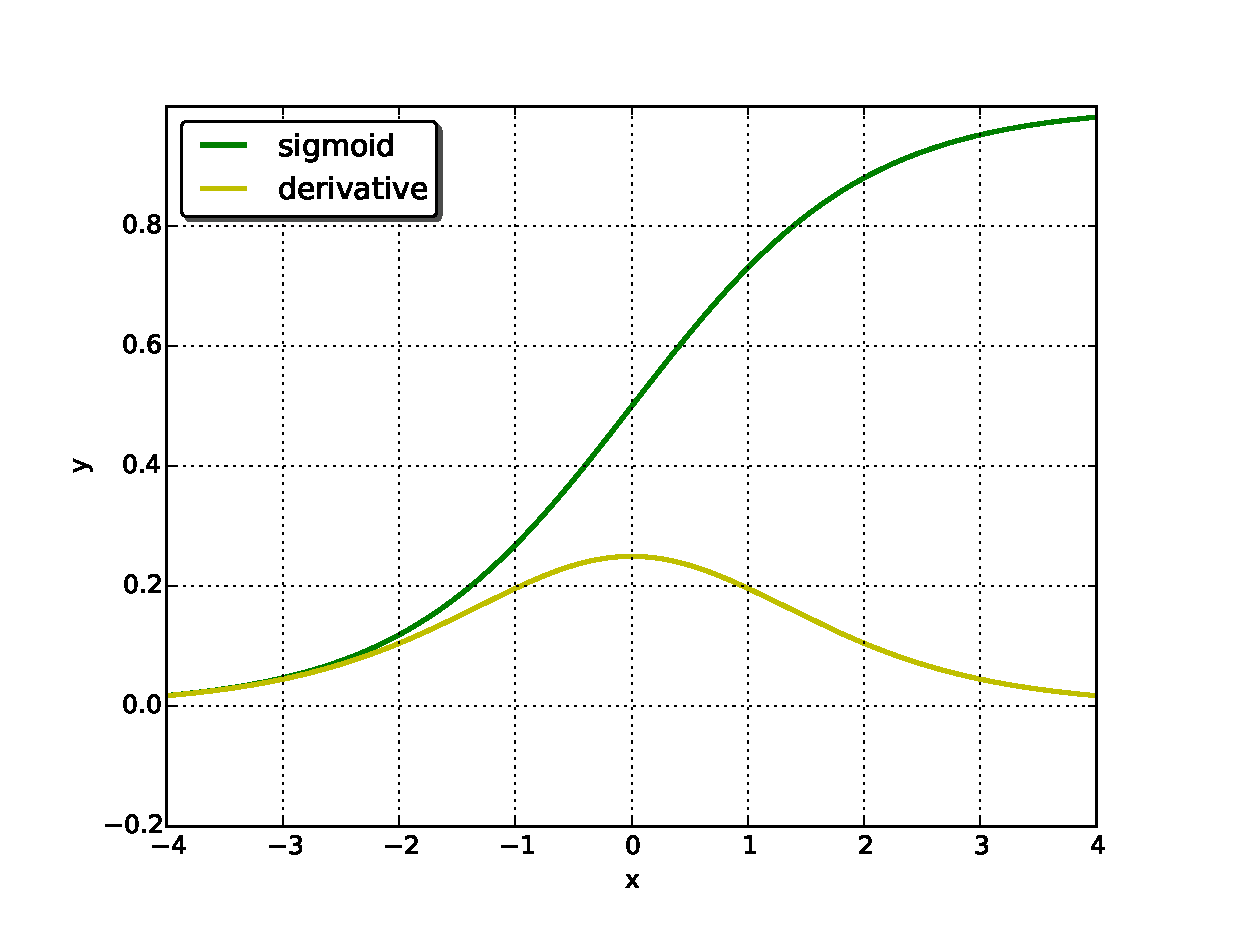
\includegraphics[width=0.9\textwidth]{sigmoid_and_deriv.eps}
  \caption{sigmoid and it's derivative}
\label{sigmoid_plot}
\end{figure}

\paragraph{Tanh}
\begin{align}
 tanh(x)&=\frac{e^x-e^{-x}}{e^x+e^{-x}} \\
 tanh'(x)&= 1 - tanh^2(x)  
\end{align}
As we can see from figure \ref{tanh_plot} tanh (and it's derivative) have a behaviour similar to the sigmoid one; Again we have two saturation region towards
infinity: that's typical of all squashing functions.



\begin{figure}[ht]
  \centering
    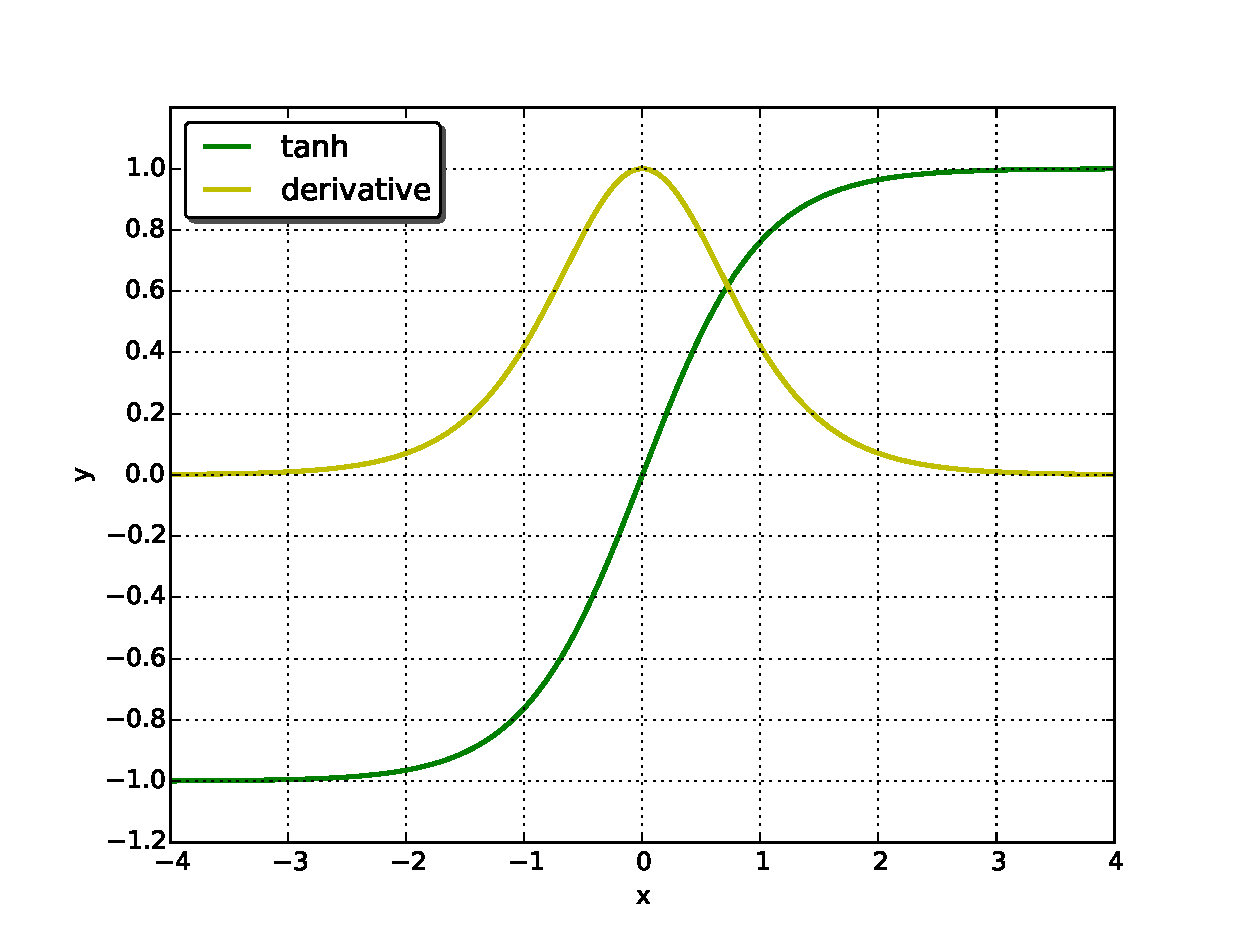
\includegraphics[width=0.9\textwidth]{tanh_and_deriv.eps}
  \caption{tanh and it's derivative}
\label{tanh_plot}
\end{figure}

\paragraph{ReLU}


\begin{align}
  ReLU(x)&=\begin{cases}
    x & \text{if $x>0$}.\\
    0 & \text{otherwise}.
  \end{cases} \\ 
   ReLU'(x)&=\begin{cases}
    1 & \text{if $x>0$}.\\
    0 & \text{otherwise}.
  \end{cases}
\end{align}
ReLU is a bit different from other activation function seen so far: the main difference is that's it's not a squashing function.
As we can see from figure \ref{relu_plot}, ReLU's derivative is the step function; it has only one \textit{saturation} region $(-\infty, 0]$ and a region in which is always takes value one, $(0,+\infty]$
This leads to the fact that we cannot learn to \textit{turn on} a switched off neuron ($x<0$), but we have no \textit{saturation} region toward infinity.

\begin{figure}[ht]
  \centering
    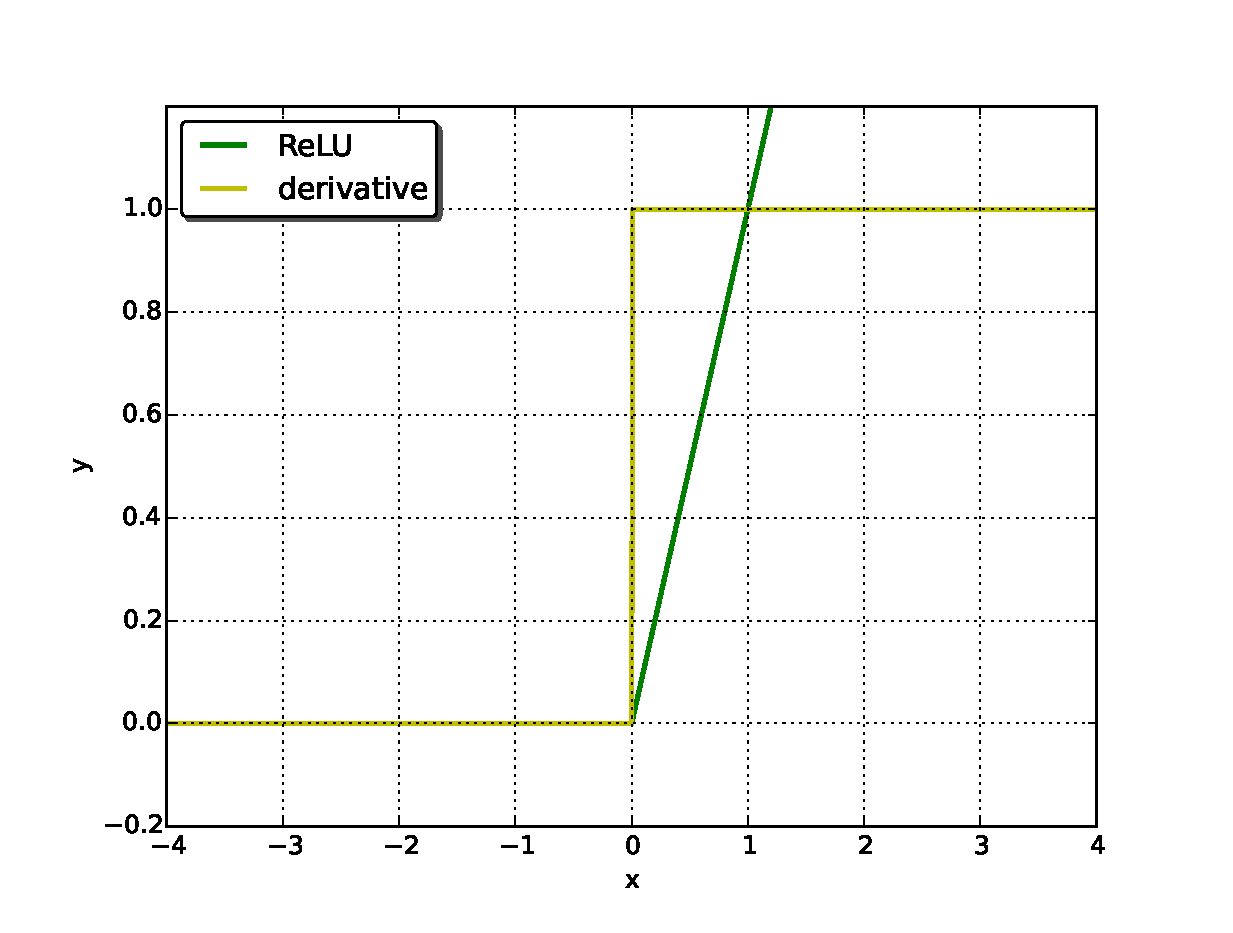
\includegraphics[width=0.9\textwidth]{relu_and_deriv.eps}
  \caption{ReLU and it's derivative}
\label{relu_plot}
\end{figure}

  \section{Stochastic gradient descent: a common framework}
  \label{sec:sgd}
In this section we will describe a framework based on gradient descent optimization method which can be used to train 
neural network of any kind. Such framework constitutes the core of many learning methods used in today's applications. 
Suppose we have a training set of pairs $D=\{\pair{\vec{x}^{(i)}}{\vec{y}^{(i)}}\}$ and a loss function $L(\theta)$ 
where $\theta$ represents all the parameters of the network.

A standard gradient descend would update $\theta$ at each iteration using the gradient computed on the whole training 
set, as shown below.
\begin{equation}
 \theta = \theta - \alpha \nabla_\theta L(\theta).
\end{equation}

This can be very slow or even impractical if the training set is too huge to fit in memory. Stochastic gradient descent (SGD)
overcome this problem taking into account only a part of the training set for each iteration, i.e. the gradient is computed only on a subset $I$ of training examples. 

\begin{equation}
 \theta = \theta - \alpha \nabla_\theta L(\theta; I)
 \label{eq:updateRule}.
\end{equation}

The subset of training examples used for the update is called \textit{mini-batch}. The number of examples for each 
mini-batch is an important hyper-parameter because it affects both the speed of convergence in terms of number of 
iterations and time needed for each iteration. At each iteration new examples are chosen among the training set, so it could, and it always does if we have a finite data-set, happen, that all training set examples get used.
This is not a problem, since we can use the same examples over and over again. Each time we go over the entire training 
set we say we completed and \textit{epoch}. It is not unusual to iterate the learning algorithm for several epochs before converging.

The method is summarized in algorithm \ref{algo:sgd}.

\begin{algorithm}[]
 \KwData{\\
 \Indp
  $D=\{\pair{\vec{x}^{(i)}}{\vec{y}^{(i)}}\}$: training set\\
  $\theta_0$: candidate solution \\
  $m$: size of each mini-batch\\
  }
  
 \KwResult{\\
 \Indp $\theta$: solution
 }
 \BlankLine
 
 $\theta \gets \theta_0$\\
 \While{stop criterion}{
 
 $I$ $\gets$ select $m$ training example $\in D$  \\
 $\alpha \gets$ compute learning rate \\
 $\theta \gets \theta - \alpha \nabla_\theta L(\theta; \pair{\vec{x}^{(i)}}{\vec{y}^{(i)}}, i\in I)$\\
 }
\caption{Stochastic gradient descent}
\label{algo:sgd}
\end{algorithm}

In the following paragraphs we will analyze in more detail each step of the method, surveying the different alternatives 
that can be used.

\paragraph{The stop criterion}

Usually a gradient based method adopts a stop criterion which allows the procedure to stop when close enough to a (local) 
minimum, i.e $\nabla_\theta L(\theta)=0$.  This could easily lead to over-fitting, so is common practice to use a 
cross-validation technique. The most simple approach to cross-validation is to split the training set in two parts, one actually used as a pool of training examples, which will be called \textit{training set}, and the other, called \textit{validation-set}, used to decide when to stop.

Being $D=\{\pair{\vec{x}^{(i)}}{\vec{y}^{(i)}}, i\in(1,M)\}$ a generic subset of the data-set, we can define the \textit{error} on such set in a straightforward manner as 

\begin{equation}
 E_D = \frac{1}{M} \sum_{i=1}^M  L(\vec{x}^{(i)},\vec{y}^{(i)})
\end{equation}

Since training examples are sampled from the training-set, the error on the training-set will always\footnote{This is not actually true; it would in a standard gradient descent, but since we are using stochastic gradient the error could be non monotonic decreasing. However the matter here is that error mainly follow a decreasing path} be decreasing across iterations. The idea behind cross-validation is to compute, and \textit{monitor} the error on the validation set, since it's not guaranteed at all that the error would be decreasing. On the contrary, tough error will generally decrease during the first part of training, it will reach a point when it will start to increase. This is the point when we need to stop training since we are starting to over-fitting. Of course this is an ideal situation, in real applications the validation error could have a more irregular trend, but the idea holds.


\paragraph{Learning rate}

The parameter $\alpha$ in Equation (\ref{eq:updateRule}) is usually referred to as \textit{learning rate}. Of course the strategy employed to compute such learning rate is an important ingredient in the learning method.
The most easy, and often preferred, strategy is that of \textbf{constant learning rate}. The learning rate $\alpha$ becomes another hyper-parameter of the network that can be tuned, but it remains constant, usually a very small value, across all iterations.

Another popular strategy is that of \textbf{momentum} which, in the optimization field is know as the \textit{Heavy 
Ball} method \cite{momentum}.
The main idea behind momentum is to accelerate progress along dimensions
in which gradient consistently point to and to slow down progress along dimensions where the sign of the gradient continues to change. This is done by keeping
track of past parameter updates with an exponential decay as shown in Equation (\ref{eq:momentum}).

\begin{align}
\label{eq:momentum}
v &= \gamma v+ \alpha \nabla_\theta L(\theta; \pair{\vec{x}^{(i)}}{\vec{y}^{(i)}}, i\in I)\\
\theta &= \theta + v
\end{align}

Another way of choosing the learning rate is to fix an initial value and \textbf{annealing} it, at each iteration (or epoch), according to a policy, for instance \textit{exponential} or \textit{linear} decay; the idea behind it being that, initially, when far from a minimum having a larger learning rate causes greater speed and after some iterations when approaching a minimum a smaller learning rate allows a finer refinement.

\textbf{Adaptive} methods, instead, choose the learning rate monitoring the objective function, hence learning rate can be reduced
or increased depending on the need, proving to be a little more versatile than annealing methods. Of course different strategies for detecting when to reduce or increase the learning rate have been devised.

Finally \textbf{line search} which is generally used when working with (non stochastic) gradient descend or when dealing with large batches. For stochastic gradient with small batches other strategies are usually 
preferred.

\paragraph{How to choose batches}

Empirical evidence has been provided that choosing a ``meaningful'' order in which examples are presented to the network can both speed the convergence and yield better solutions. Generally speaking, the network can learn faster if trained first with easier examples and then with examples with gradually increasing difficulty, as humans or animals would do. The idea was introduced by Bengio et al.\cite{curriculumLearning} in 2009, as \textit{curriculum} learning. Experiments on different curriculum strategies can be found in \cite{learningToExecute}.


  \section{The vanishing and exploding gradient problem}
    \label{sec:vanishing}
    We have seen in the previous section that
\begin{equation}
\frac{\partial \vec{a}^t}{\partial \vec{a}^k} = \prod_{i=t-1}^{k}  diag(\sigma'(\vec{a}^i)) \cdot \mat{W}^{rec}
\end{equation}

In an equivalent way with can rewtite the previous equation with respect to a couple of neurons $i$ and $j$

\begin{equation}
\frac{\partial \vec{a}_i^t}{\partial \vec{a}_j^k} = \sum_{q\in P(j)} \sum_{l \in P(q)} \hdots \sum_{h : i \in P(h)} w_{qj} \hdots w_{jh} \cdot \sigma'(a_j^k)\sigma'(a_q^{k+1}) \hdots \sigma'(a_i^{t-1})
\label{expanded_mem}
\end{equation}


Observing the previous equation we can argue that each derivatives it's the sum of $p^{t-k-1}$ terms; each term represents the path cost from neuron $i$ to neuron $j$ in the unfolded network, obviously
there are $p^{t-k-1}$ such paths. If we bind the cost $\sigma'(a_l^t)$ to neuron $l$ in the $t^{th}$ layer in the unfolded network we can read the path cost simply surfing the unfolded network multiply
the weight of each arc we walk through and the cost of each neuron we cross, as we can see from figure \ref{gradient_path_cost}.


\tikzstyle{rnn_style}=[->,shorten >=1pt,auto,node distance=1.5cm,
  thick,
  neuron/.style={circle,fill=white!50,draw,minimum size=0.7cm,inner sep=0pt,font=\sffamily\normalsize},
  missing/.style={circle,fill=white!50,draw=none,minimum size=0.7cm,font=\sffamily\Huge\bfseries},
  label/.style={node distance=1.2cm,rectangle,fill=white!50,draw=none,minimum size=0.7cm,font=\sffamily\normalsize},
  thick_edge/.style={line width=1.2pt},
  thin_edge/.style={dotted, line width=0.5pt},
  weight/.style = {above,sloped,pos=0.3},
  ]
\begin{figure}
 \centering
\begin{tikzpicture}[rnn_style]

  
  \node[neuron]    (x1)[]   {$\sigma_1^t$};
  \node[neuron]    (x2)[right of=x1]   {};
  \node[neuron]    (x3)[right of=x2]   {};
  \node[label]     (xl)[left of=x1] {$t$};
  
  \node[neuron]    (h1)[below of =x1]   {$\hdots$};
  \node[neuron]    (h2)[right of=h1]   {};
  \node[neuron]    (h3)[right of=h2]   {};
  \node[label]     (hl)[left of=h1] {$\hdots$};
  
  \node[neuron]    (y1)[below of=h1]   {};
  \node[neuron]    (y2)[right of=y1]   {};
  \node[neuron]    (y3)[right of=y2]   {$\sigma_3^{k+2}$};
  \node[label]     (yl)[left of=y1] {$k+2$};

  
  \node[neuron]    (z1)[below of=y1]   {$\sigma_1^{k+1}$};
  \node[neuron]    (z2)[right of=z1]   {};
  \node[neuron]    (z3)[right of=z2]   {};
  \node[label]     (zl)[left of=z1] {$k+1$};
  
  \node[neuron]    (w1)[below of=z1]   {};
  \node[neuron]    (w2)[right of=w1]   {$\sigma_2^k$};
  \node[neuron]    (w3)[right of=w2]   {};
  \node[label]     (wl)[left of=w1] {$k$};

  
%   \node[label]      (lu)[left of=u] {$u$};
%   \node[label]      (ll)[left of=z1] {$l$};


  \path[->] (h1) edge [thick_edge] node[weight]{$w_{11}$}  (x1)
	    (h1) edge [thin_edge]   (x2)
	    (h1) edge [thin_edge]   (x3)
	    (h2) edge [thin_edge]  (x1)
	    (h2) edge [thin_edge]   (x2)
	    (h2) edge [thin_edge]   (x3)
	    (h3) edge [thin_edge]  (x1)
	    (h3) edge [thin_edge]   (x2)
	    (h3) edge [thin_edge]   (x3);

  \path[->] (y1) edge [thin_edge]   (h1)
	    (y1) edge [thin_edge]   (h2)
	    (y1) edge [thin_edge]   (h3)
	    (y2) edge [thin_edge]   (h1)
	    (y2) edge [thin_edge]   (h2)
	    (y2) edge [thin_edge]   (h3)
	    (y3) edge [thick_edge] node[weight]{$w_{13}$}   (h1)
	    (y3) edge [thin_edge]   (h2)
	    (y3) edge [thin_edge]   (h3);
  
  
  \path[->] (z1) edge [thin_edge]   (y1)
	    (z1) edge [thin_edge]  (y2)
	    (z1) edge [thick_edge] node[weight]{$w_{31}$}   (y3)
	    (z2) edge [thin_edge]  (y1)
	    (z2) edge [thin_edge]  (y2)
	    (z2) edge [thin_edge]  (y3)
	    (z3) edge [thin_edge]   (y1)
	    (z3) edge [thin_edge]   (y2)
	    (z3) edge [thin_edge]   (y3);
	    
  \path[->] (w1) edge [thin_edge]   (z1)
	    (w1) edge [thin_edge]  (z2)
	    (w1) edge [thin_edge]   (z3)
	    (w2) edge [thick_edge] node[weight]{$w_{12}$}   (z1)
	    (w2) edge [thin_edge]   (z2)
	    (w2) edge [thin_edge]   (z3)
	    (w3) edge [thin_edge]   (z1)
	    (w3) edge [thin_edge]   (z2)
	    (w3) edge [thin_edge]   (z3);

	    


\end{tikzpicture}
\caption{The cost for a path from neuron $2$ at time $k$ to neuron $1$ at time $t$ is $w_{12}w_{31}w_{13}\hdots w_{11}\cdot \sigma_2^k \sigma_1^{k+1}\sigma_3^{k+2} \hdots \sigma_1^{t-1} $ }
\label{gradient_path_cost}
\end{figure}


We can further characterize each path cost noticing that we can separate two components, one that depends only on the weights $w_{qj} \hdots w_{jh}$ and the other that depends both on the weights and the inputs
$\sigma'(a_j^k)\sigma'(a_q^{k}) \hdots \sigma'(a_i^{t-1})$.


\paragraph{Hochreiter Analysis: Weak upper bound}

Let's put $$\sigma'_{max} \triangleq \underset{i=k,...,t-1}{\text{max  }} \{||diag(\sigma'(a^i))||_1\}$$.

We have then:
$$\left\Vert \prod_{i=t-1}^{k}  diag(\sigma'(\vec{a}^i)) \cdot \mat{W}^{rec} \right\Vert_1 <= \prod_{i=t-1}^{k} p \cdot ||diag(\sigma'(\vec{a}^i))||_1 \cdot ||\mat{W}^{rec}||_1 $$
since 
$$||diag(\sigma)\cdot \mat{W}||_1 =
\left\Vert 
\begin{array}{c c c c}
\sigma_1 w_{11} & \sigma_1 w_{12} & \hdots & \sigma_1 w_{1p}  \\
\sigma_1 w_{21} & \sigma_2 w_{22} & \hdots & \sigma_2 w_{2p}  \\
\vdots & \vdots  & \vdots & \vdots  \\
\sigma_p w_{p1} & \sigma_p w_{p2} & \hdots & \sigma_p w_{pp}  \\
\end{array}  
\right\Vert_1
<=p \cdot \sigma_{max} \cdot ||\mat{W}||_1
$$

Hence
\begin{align}
\left\Vert \prod_{i=t-1}^{k}  diag(\sigma'(\vec{a}^i)) \cdot \mat{W}^{rec} \right\Vert_1 & <= p \cdot \big(\sigma'_{max}\cdot ||\mat{W}||_1\big)^{t-k-1} \\
& = p \cdot \tau^{t-k-1}
\end{align}
where $$\tau \triangleq \sigma'_{max}\cdot ||\mat{W}||_1$$

So we have exponential decay if $\tau<1$; We can match this condition assuring that
$$\frac{p\cdot ||w_{max}||}{\sigma_{max}}<1$$ where $w_{max}$ is the maxixum value in the weight matrix.


COMPORTAMENTO SBALIATO STRUTTURALE\\
RELU-NON POSSIAMO IMPARARE AD ACCENDERE \\
MEMORIA\\





  \section{On expressiveness}
  \label{sec:expressiveness}
  In this section we will investigate the expressive power of neural networks, presenting some results that motivate the use of neural networks as learning
model; we will also show how different architectures leads to different kind of computational power.
 

Maybe the most important result regarding the expressive power of neural networks it's due to Hornik et al. \cite{Hornik89} which basically states
\textit{'Multilayered feed foward networks with at least one hidden layer, using an arbitrary squashing function can approximate virtually any function
of interest to any desired degree of accuracy provided sufficiently many hidden units are available'}.

To give a more formal result we need first to define what \textit{approximate to any degree of accuracy means}, this concept is captured in definition
\ref{dens_compact}
 
\begin{defn}
 A subset S of $\mathbb{C}^n$ (continuoos functions in $\mathbb{R}^n$) is said to be \textit{uniformly dense on compacta in} $\mathbb{C}^n$ if $\forall$
 compact set $K\subset \mathbb{R}^n$ holds: $\forall \epsilon >0$, $\forall g(\cdot) \in \mathbb{C}^n$ $\exists f(\cdot) \in S$ such that 
 $\underset{x \in K}{\text{sup  }} \norm{f(x)-g(x)}<\epsilon$ 
 \label{dens_compact}
\end{defn}

Hornik result is contained in theorem \ref{universal_approx}.
\begin{thm}
 For every activation function $\sigma$, $\forall n\in \mathbb{N}$, feed foward neural
 networks with one hidden layer are a class of functions which is \textit{uniformly dense on compacta in} $\mathbb{C}^n$
\label{universal_approx}.
\end{thm}
Therem \ref{universal_approx} extends also to Borel measurable functions, please see \cite{Hornik89} for more details.


This result implies that FNN are \textit{universal approximators}, this is a strong argument for using such models in machine learning.
It's important to notice, however, that the theorem holds if we have \textit{sufficiently many} units. In praticice the number of units will bounded
by the machine capabilities and by computational time, of course greater the number of units greater will be the learning time. This will limit
the expressiveness of the network to a subset of all measurable functions.

\\\\POGGIO GIROSI?

\\\\RNNs


\chapter{Literature review}
  
Hochreiter\cite{lstm} in 1991, Bengio et al.\cite{learningIsDifficult} in 1994, and others, observed that gradient in 
deep neural networks tends to either vanish or explode. From then onward several methods have been proposed to 
overcome what is now know as the \textit{exploding/vanishing gradient} problem. We can roughly partition such methods in 
two broad categories.
The approaches of the first kind, the ones we will call \textit{architectural driven}, usually use a simple stochastic gradient descend (SGD) as learning algorithm, and act on the network topology, modifying the way the 
neural units operates, the connections between them or the relationship between layers; the idea of such methods is to 
build networks architectures in which gradient are less likely to vanish, or in other words whose units are able to 
store information for several time steps.

The second approach, which we'll call \textit{learning driven}, instead, focus on the learning algorithm, leaving the 
network architecture untouched. Methods belonging to these categories, either employ learning algorithms different from 
SGD, or they propose modification to the SGD framework.


In the rest of the chapter we will review the most relevant approaches for both the categories.

  \section{Architectural driven methods}
  
\subsection{Long short-term memory} 

\textit{Long short-term memory} (LSTM) were proposed (1997) by Hochreiter and Schmidhuber\cite{lstm} as a novel network 
structure to address the vanishing gradient problem, which was first studied by Hochreiter (1991) in his diploma 
thesis, a milestone of deep learning.

The idea behind this structure is to enforce a constant error flow, that is to say, to have constant gradient norm, 
thus preventing the gradient to vanish. This is done by introducing special types of neurons called \textit{memory 
cells} and \textit{gate units}. As we can see by looking at Figure \ref{lstm_neuron}, a memory cell is essentially a 
neuron with a self connection with unitary weight, whose input and output are managed by two multiplicative neurons: 
the gate units.


\tikzstyle{nn_style}=[->,shorten >=1pt,auto,node distance=1.5cm,
  thick,
  neuron/.style={circle,fill=white!50,node distance=1cm,draw,minimum size=0.7cm,font=\sffamily\normalsize},
  missing/.style={circle,font=\sffamily\Large,node distance=0.95cm},
  label/.style={node distance=1.2cm,rectangle,fill=white!50,draw=none,minimum size=0.7cm,font=\sffamily\normalsize},
  layer/.style={rectangle,fill=white!50,draw,minimum width=0.8cm,font=\sffamily\Large},
  loopStyle/.style={in=120,out=60, distance=2.5cm},
  weight/.style = {above,sloped,pos=0.3},]
\begin{figure}[h]
  \centering
  \begin{tikzpicture}[nn_style]

    %horizontal line
    \node[neuron]	(c1)       					{$\times$};
    \node[layer] 	(s_mem)	[right of=c1,	node distance=1.5cm] 	{$\Sigma$};
    \node[neuron]	(mem)	[right of=s_mem,node distance=1.5cm]	{$m_j$};
    \node[layer] 	(h)	[right of=mem,	node distance=1.5cm] 	{$h$};
    \node[neuron]	(c2)	[right of =h,	node distance=1.5cm]	{$\times$};
    \node[label]  	(out)	[right of=c2,	node distance=2.2cm]	{$h_j$};
    
    \path[->] (c1) 	edge []   (s_mem)
	      (s_mem) 	edge []   (mem)
	      (mem) 	edge []   (h)
	      (h) 	edge []   (c2)
	      (c2) 	edge []   (out);
	     
    
    %loop	     
    \path[->] (mem) edge [loop, in=90,out=120, distance=0.8cm, anchor=south ] node [align=center, pos=0.7] 
 {$1$} (s_mem);

    
    %above inputs
    \node[layer] 	(g)	[above of=c1,	node distance=1.5cm] 	{$g$};
    \node[layer] 	(s_in)	[above of=g,	node distance=1.2cm] 	{$\Sigma$};
    \node[missing]	(i2)	[above of=s_in, node distance=1.2cm]	{$\hdots$};
    \node[neuron]	(i3)	[right of=i2, 	node distance=1cm]	{};
    \node[neuron]	(i1)	[left of=i2, 	node distance=1cm]	{};

    
    \path[->] (s_in) 	edge [anchor=west]	node[]{}	(g)
	      (g) 	edge [anchor=west]   	node[]{$a_j$}	(c1)
	      (i1)	edge []   					(s_in) 
      	      (i3)	edge []   					(s_in);
      	      
      	      
    %below gate input unit
    \node[layer] 	(sig_in)	[below of=c1,		node distance=1.5cm] 	{$\sigma$};
    \node[layer] 	(s_gate_in)	[below of=sig_in,	node distance=1cm] 	{$\Sigma$};
    \node[missing]	(gi2)		[below of=s_gate_in, 	node distance=1.2cm]	{$\hdots$};
    \node[neuron]	(gi3)		[right of=gi2, 		node distance=1cm]	{};
    \node[neuron]	(gi1)		[left of=gi2, 		node distance=1cm]	{};

    
    \path[->] (s_gate_in) 	edge [anchor=west]	node[]{}	(sig_in)
	      (sig_in) 		edge [anchor=west]	node[]{$u_j$} 	(c1)
	      (gi1)		edge []   (s_gate_in) 
      	      (gi3)		edge []   (s_gate_in);
      	      
      	      
    %below gate output unit
    \node[layer] 	(sig_out)	[below of=c2,		node distance=1.5cm] 	{$\sigma$};
    \node[layer] 	(s_gate_out)	[below of=sig_out,	node distance=1cm] 	{$\Sigma$};
    \node[missing]	(go2)		[below of=s_gate_out, 	node distance=1.2cm]	{$\hdots$};
    \node[neuron]	(go3)		[right of=go2, 		node distance=1cm]	{};
    \node[neuron]	(go1)		[left of=go2, 		node distance=1cm]	{};

    
    \path[->] (s_gate_out) 	edge [anchor=west]	node[]{}	   (sig_out)
	      (sig_out) 	edge [anchor=west]	node[]{$o_j$}   (c2)
	      (go1)		edge []						   (s_gate_out) 
      	      (go3)		edge []						   (s_gate_out);

    %enclosing rectangle
    \node[rectangle,dashed,fill=none,draw,minimum height=3.2cm,minimum width=8.1cm] at (3.4, 0.5) (memoryCell)	{};
    \node[label]  (memoryLabel)	at(3.5,2.1)	{Memory cell};


      	      
\end{tikzpicture}
\caption{Memory cell and gate units of LSTM network.}
\label{lstm_neuron}
\end{figure}

The memory cell and the gate units behave accordingly to the following:

\begin{align}
&u_j^t = \sigma[\mat{W_u}\cdot\vec{x_t} + \mat{U}_u\cdot\vec{h}_{t-1}]_j \\
&o_j^t = \sigma[\mat{W_o}\cdot\vec{x_t} + \mat{U}_o\cdot\vec{h}_{t-1}]_j \\
&a^t_j\defeq g[\mat{W}\cdot\vec{x_t} + \mat{U}\cdot h_i^t]_j\\
\label{mem_update}
&m_j^t\defeq a_j\cdot u_j^t + (1 \cdot m_j^{t-1})\\
&h_j\defeq h(m_j^t)\cdot o^t_j.
\end{align}


% \begin{equation}
% u^t_j\defeq \sigma(\sum_i w_{ui}\cdot u^{t-1}_j)
% \end{equation}
% \begin{equation}
% o^t_j\defeq \sigma(\sum_i w_{oi}\cdot o^{t-1}_j)
% \end{equation}
% 
% 
% \begin{equation}
% a^t_j\defeq g(\sum_i w_{ij}\cdot \phi_i^t)
% \end{equation}
% \begin{equation}
%  m_j^t\defeq a_j\cdot u_j^t + (1 \cdot m_j^{t-1})
% \label{mem_update}
% \end{equation}
% \begin{equation}
%  \phi_j\defeq h(m_j^t)\cdot o^t_j
% \end{equation}

As we can see from Equation (\ref{mem_update}), the value of the memory cell $m(t)$ remains constant as long as the input 
gate $u$ does not ``open'' causing a ``write'' operation. Similarly the output $o$ of the memory cell, which is 
connected with 
the other neurons of the network, is controlled by an output gate: the memory will have a non zero output only if the 
output gate opens, which we could call a ``read'' operation. As for constant error flow it is ensured because the 
memory cell has only a self-loop with unitary weight.

Memory cells, guarded by gate units can be employed in networks with various topology alongside traditionally 
input, output and hidden units. Another way to look at this kind of architecture is to think of memory cells as units 
able to store one bit of information, even for long periods of time, hence able to learn distant time correlations 
between inputs.

As we have seen these network units are specifically designed to store information, through the use of gates; these 
gates however are no different from other units, apart from the fact they are multiplicative units, hence without 
further precautions, the networks would incur in the same vanishing problem it aimed to resolve. In fact LSTM comes with 
a proper, specifically designed, learning algorithm: essentially errors, i.e. gradients of the loss function, arriving at memory cells inputs are not propagated back in time, only 
the error within the memory cell gets propagated; in other words gradients are truncated taking into account only the 
self-connection of the memory cells and not its other input connections, hence providing constant error flow.
\\\\
LSTM units have proven to be very successful reaching state-of-art results in various tasks and even at the present time (2015), they continue to be largely
employed. In recent implementations however, alongside small modifications, as the introduction of other gates, the LSTM architecture is often used without the original learning algorithm which is often replaced by a standard stochastic gradient descend as done in \cite{lstmGraves}.








   
\subsection{Gated recurrent units}

Gated recurrent units (GRU) were introduced by Cho et al.\cite{gru} in 2014  as units similar to LTSM, with the same purpose, 
but claimed to simpler to compute and implement. A GRU unit $j$ make use of two gate units, $z$, the 
\textit{update} gate, and $r$, the \textit{reset} gate, which are standard neurons.
\begin{align}
 &z_j^t = [\sigma(\mat{W_z}\vec{x_t} + \mat{U}_z\vec{h}_{t-1})]_j\\
 &r_j^t = [\sigma(\mat{W_r}\vec{x_t} + \mat{U}_r\vec{h}_{t-1})]_j.\\
\end{align}
As in LSTM units, the gates manage the access to memory cell, but in GRU they are used a little bit 
differently. The update gate is used to decide how to update the memory cell: the activation value of the cell 
$h_j^{t}$ is a linear interpolation between the previous activation $h_j^{t-1}$ and the candidate activation 
$\tilde{h}_j^t$.
\begin{align}
 &h_j^t \defeq (1-z_j^t)h_j^{t-1} + z_j^t\tilde{h^t_j}\\
  \label{candidateEq}
 &\tilde{h}_j^t = [\sigma(\mat{W}\vec{x_t} + \mat{U}(\vec{r}_t \odot \vec{h}_{t-1})]_j
\end{align}
where $\odot$ symbolize the element-wise product.

As we can see from Equation (\ref{candidateEq}), when the reset gate $r_j^t$ is close to zero, the units acts as if 
reading the first symbol of the input sequence \textit{forgetting} the previous state.

\paragraph{Architecture comparison}
LSTM and GRU present very similarities, the most relevant one being the additive mechanism of update which helps the 
networks to store information during several time step. One difference between the two architectures is, instead, the 
lacking of an output gate in GRU, which hence expose the content of the memory cell without any supervision. In 
\cite{gru_lstm_empirical} Cho et al. compare the two architectures showing how a gated architecture improves the 
performance of a network composed of traditional units; The comparison results obtained were however mixed, and in the 
end they could not demonstrate the superiority of one of the two approaches.

In 2015 an interesting work\cite{architectureMutations} was done  on neural network architectures. The aim of the work was to determine if LSTM or GRU were optimal, or whether a better architecture exists. This was accomplished by comparing thousands of randomly generated architectures using the best hyper-parameter setting for each one. The architectures were generated randomly mutating a given architecture, replacing its activation function nodes, choosing from ReLU, tanh, sigmoid etc., and its operation nodes, with multiplication, subtraction or addition. The result of the experiment is that no one of mutated architectures constantly performed better than LTSM and GRU in all the considered tasks. Moreover the best randomly generated architectures were very similar to the GRU architecture. The conclusion drawn in \cite{architectureMutations}  is that architectures better than LSTM and GRU  either do not exist or are difficult to find. 
  \subsection{Structurally constrained recurrent network}

In 2015 Mikolov proposed a novel network architecture to deal with vanishing gradients \cite{scrn} called 
\textit{Structurally constrained recurrent network} (SCRN). The idea is to introduce a hidden layer specifically 
designed to capture long-term dependencies alongside the traditional one as shown in Figure \ref{fig:scrn}.


\tikzstyle{rnn_style}=[->,shorten >=1pt,auto,node distance=1.5cm,
  thick,
  neuron/.style={circle,fill=white!50,draw,node distance = 1cm, minimum size=0.7cm,font=\sffamily\Large\bfseries},
  gate/.style={circle,fill=white!50,draw,node distance = 1cm,font=\sffamily\small\bfseries},
  missing/.style={rectangle,fill=white!50,node distance =1cm,draw=none,minimum size=0.7cm,font=\sffamily\Huge\bfseries},
  label/.style={node distance=1.2cm,rectangle,fill=white!50,draw=none,minimum size=0.7cm,font=\sffamily\normalsize},
  layer/.style={rectangle,fill=white!50,draw,minimum width=3.5cm,minimum height=0.5cm, font=\sffamily\normalsize},]
\begin{figure}[!ht]
 \centering
\begin{tikzpicture}[rnn_style]
  
  \node[layer] (x)[] {input layer};
  \node[layer] (h)[above left =1.2cm and -1.5cm of x] {hidden layer};
  \node[layer] (s)[above right =1.2cm and -1.5cm of x] {context layer};
  \node[layer] (y)[above right = 1.2cm and -1.5cm of h,] {output layer};
  
  \node[label] (xLabel) [below of=x, node distance=1.2cm]{$\vec{x}$};
  \node[label] (yLabel) [above of=y, node distance=1.2cm]{$\vec{y}$};

  
    \path[->] (x) edge 	[] node[]{}   	(h)
	    (x) edge 	[]   		(s)
	    (h) edge	[]		(s)
	    (h) edge[]			(y)
	    (s) edge[]			(y)
	    (xLabel)edge[]		(x)
	    (y)edge[]		(yLabel)
	    (h.north)edge[bend right=120, distance = 3.5cm]	(h.south)
	    (s.north)edge[bend left=120, distance = 3.5cm]	(s.south);
	    


\end{tikzpicture}
\caption{SCRN architecture.}
\label{fig:scrn}
\end{figure}


As observed in \cite{scrn}, and explained in section \ref{sec:vanishing}, gradient can vanish either because of the 
non linearities being all close to 0 or because of the multiplication of the weight matrix at each time step. The proposed 
layer, called \textit{context layer}, address these problem by completely removing the non linearity and forcing the 
recurrent matrix to be close to the identity. Formally the context layer  $\vec{s}$ is given by:

\begin{equation}
 \vec{s}_t = (1-\alpha)\mat{B}\vec{x}_t + \alpha\vec{s}_{t-1}.
\end{equation}

The rest of the network is like a traditional one, hence, adding the context layer beside the traditional one results 
in:
\begin{align}
 &\vec{h}_t = \sigma(\mat{P}\vec{s}_t + \mat{A}\vec{x}_t + \mat{R}\vec{h}_{t-1})\\
 &\vec{y}_t = f(\mat{U}\vec{h}_t + \mat{V}\vec{s}_t).
\end{align}
Notice the similarity with leaky integrator units \cite{leakyIntegratorUnits}.

If we treat context and traditional layers as one, i.e we do not distinguish between context and traditional units, we can 
see the model as a traditional model whose recurrent matrix $\mat{W}$ is constrained (from this the name of the 
method), to be of the form:
\begin{equation}
 \mat{W} =  \begin{bmatrix}
R & P \\
0 & \alpha I
\end{bmatrix}
\end{equation}
Matrix $\mat{W}$ is a traditional recurrent matrix constrained to have a diagonal block to be equal to a weighted 
identity. 

Observing that fixing $\alpha$ to be constant makes the context units to work on the same time scale, Mikolov propose 
to have a different value for each unit, hence allowing to capture context from different time delay.
\begin{equation}
  \vec{s}_t = (\mat{I}-\mat{Q})\mat{B}\vec{x}_t + \mat{Q}\vec{s}_{t-1}
\end{equation}
where $\mat{Q}\defeq diag(\sigma(\vec{\beta}))$; the vector $\vec{\beta}$ is learned.

In \cite{scrn} SCRNs are shown to be roughly equivalent to the much more complex, LSTMs.



  \subsection{Gated feedback recurrent neural networks}

\textit{Gated feedback recurrent neural networks} were proposed in 2015 by  Chung et al. \cite{gatedFeedback} as a novel recurrent network architecture.
Unlike LSTM or GRU where the novelty of the proposal was a new kind of unit, designed to better capture long-term dependencies between inputs, the novelty of this approach is the way the units are arranged. For starters multiple recurrent layer are used, like in a \textit{Stacked RNN}, i.e. the network is composed of several layers, each one of which is connected to all the others; in other words the layers are fully connected. Moreover, unlike traditional stacked RNNs, the feedback connection between different layers is gated by a \textit{global reset gate} which is essentially a logistic unit computed on the current inputs and the previous states of hidden layers. This global reset gates is reminiscent of the gates of LSTM and GRU but it controls the connection between layers not between units: the hidden state values of layer $i$ at time $t-1$ are fed to a lower layer $j$ multiplied by $g^{i\rightarrow j}$.
The gate between layers $i$ and $j$ is computed as:
\begin{equation}
g^{i\rightarrow j} \defeq \sigma(\vec{w}_g^{i\rightarrow j} \cdot \vec{h_t}^{j-1} + \vec{u}_g^{i\rightarrow j} \cdot \vec{h}^*_{t-1})
\end{equation}
where $\vec{w}_g^{i\rightarrow j}$ and $\vec{u}_g^{i\rightarrow j}$ are the weights of the links between the gate and the input and the hidden states of all layers at time-step $t-1$ respectively; for $j=1$,  $\vec{h}_t^{j-1}=\vec{x}_t $  and $\vec{h^*_{t-1}}$ represents all the hidden states at time $t-1$.

The idea behind this architecture is to encourage each recurrent layer to work at different timescales, hence capturing both long-term and short-term dependencies. In addition, the units composing the layers, can be traditional sigmoidal units but also LSTM or GRU, hence benefiting from both the strength of these kind of units and the global gate mechanism. In \cite{gatedFeedback} the architecture is evaluated against traditional and stacked RNNs with both LSTM and GRU units: gated feedback networks are shown to offer better performance and accuracy in several challenging tasks.


\tikzstyle{rnn_style}=[->,shorten >=1pt,auto,node distance=1.5cm,
  thick,
  neuron/.style={circle,fill=white!50,draw,node distance = 1cm, minimum size=0.7cm,font=\sffamily\Large\bfseries},
  gate/.style={circle,fill=white!50,draw,node distance = 1cm,font=\sffamily\small\bfseries},
  missing/.style={rectangle,fill=white!50,node distance =1cm,draw=none,minimum size=0.7cm,font=\sffamily\Huge\bfseries},
  label/.style={node distance=1.2cm,rectangle,fill=white!50,draw=none,minimum size=0.7cm,font=\sffamily\normalsize},
  layer/.style={rectangle,fill=white!50,draw,minimum width=4cm,minimum height=0.5cm, font=\sffamily\normalsize},
  gateEdge/.style={dotted},]
\begin{figure}
 \centering
\begin{tikzpicture}[rnn_style]
  
  \node[layer] (l1)[] {$L_1$};
  \node[missing] (l2)[above of=l1,node distance=1.2cm]{$\hdots$};
  \node[layer] (l3)[above of=l2,node distance=1.2cm] {$L_3$};
  \node[layer] (l4)[above of=l3,node distance=1.2cm] {$L_4$};
  
  \node[label] (x) [below of=l1, node distance=1.2cm]{$\vec{x}$};
  \node[label] (y) [above of=l4, node distance=1.2cm]{$\vec{y}$};

  
    \path[->] (l1) edge 	[] node[]{}   	(l2)
	    (l2) edge 	[]   		(l3)
	    (l3) edge	[]		(l4)
	    (x) edge[]			(l1)
	    (l4) edge[]			(y);
  
  \node[gate] (g44)[left of=l4, node distance =3cm]{$g_{44}$};
  \node[gate] (g43)[left of=l3, node distance =3cm]{$g_{43}$};
  \node[gate] (g41)[left of=l1, node distance =3cm]{$g_{41}$};
  \node[gate] (g33)[right of=l3, node distance =3cm]{$g_{33}$};
  \node[gate] (g31)[right of=l1, node distance =3cm]{$g_{31}$};
  \node[gate] (g11)[below of=g31, node distance =1.3cm]{$g_{11}$};
  
      \path[->] (g44) edge[gateEdge]   		(l4)
		(l4.north)  edge[gateEdge,bend right=50] (g44.north)
		(l4.north)  edge[gateEdge,bend right=90,distance=2.8cm] (g43.west)
		(g43) edge[gateEdge]		(l3)
		(l4.north)  edge[gateEdge,bend right=100, distance =4.5cm] (g41.west)
		(g41) edge[gateEdge]		(l1)
		(l3.east)  edge[gateEdge,bend left=50, anchor=east]	(g33)
		(g33) edge[gateEdge]		(l3)
		(l3.east)  edge[gateEdge,bend left]	(g31.north)
		(g31) edge[gateEdge]		(l1)
		(l1.east) edge[gateEdge, bend left]		(g11.north)
		(g11) edge[gateEdge, bend left]		(l1);

\end{tikzpicture}
\caption{Gated feedback architecture. Only connections between layers are shown, dotted when trough gates.}
\label{fig:gated}
\end{figure}


  \section{Learning driven methods}
  \subsection{Preserve norm by regularization and gradient clipping} 

In 2013 Pascanu \cite{pascanu} proposed a regularization term $\Omega$ for the loss function $L(\theta)$ which should address the vanishing gradient problem.
The objective function hence become:
\begin{equation}
 \tilde{L}(\theta) \defeq L(\theta) + \lambda\Omega(\theta)
\end{equation}

Such a term represents a preference for solutions such that back-propagated gradients preserves norm in time.
\begin{equation}
\Omega = \sum_t \left( \frac{\norm{ \frac{\partial L}{\partial \vec{h}_{t+1}} \cdot \frac{\partial \vec{h}_{t+1}}{\partial \vec{h}_t} }}{\norm{\frac{\partial L}{\partial \vec{h}_{t+1}}}} -1  \right)^2 
\label{eq:pascanuReg}
\end{equation}

As we can see from equation \ref{eq:pascanuReg} the regularization term forces $\frac{\partial \vec{h}_{t+1}}{\partial \vec{h}_t}$ to preserve norm in the relevant direction of the error $\frac{\partial L}{\partial \vec{h}_{t+1}}$.

The intuition behind this technique is that $\frac{\partial \vec{h}_{t}}{\partial \vec{h}_k}$ measure the dependence of outputs at time $t$ on the previous time steps $t-1,...k$. In \cite{pascanu} is argued that even though some precedent inputs $k<t$ will be irrelevant for the prediction of time time $t$, the network cannot learn to ignore them unless there is an error signal; hence it's a good idea to force the network to increase $\frac{\partial \vec{h}_{t}}{\partial \vec{h}_k}$, even at the expense of greater error of the loss function $L(\theta)$, and then wait for it to learn to ignore these inputs.

As for the exploding vanishing gradient, in \cite{pascanu} is argued that a simple method called \textit{gradient clipping}, first used by Mikolov\cite{clippingMikolov}, can be effective against exploding gradient. The method, shown in algorithm \ref{algo:gradClipping}, simply consists in rescale the gradient norm when it goes over a threshold.

\begin{algorithm}[]
$\vec{g} \gets \nabla_{\theta} L$\\
\If{$\norm{\vec{g}} \geq threshold $}{$\vec{g} \gets \frac{threshold}{\norm{\vec{g}}} \vec{g}$}
\caption{Gradient clipping}
\label{algo:gradClipping}
\end{algorithm}

A drawback of such an approach is the introduction of another hyper-parameter, the threshold, however in \cite{pascanu} is said that a good heuristic
is to choose a value from half to ten time the average gradient norm over a sufficiently large number of updates.
The algorithm can be described also in term of adjusting the learning rate monitoring the gradient. Our understanding is that such escamotage is not necessary at all when, for instance, using a line search algorithm for setting the learning rate.
  \subsection{Hessian-free optimization}

During 2010-2011 Martens and Sutskever\cite{hessianFree} proposed an developed an hessian-free method for recurrent neural network training.
The proposal consists in using hessian-free optimization with some crucial modifications which make the approach suitable for recurrent neural networks.

As in  the classical Newton's method the idea is to iteratively compute the updates to parameter $\theta$ by minimizing a local quadratic approximation $M_{k}(\delta)$ of the objective function $f(\theta_k +\delta)$, which in the case of RNNs is the loss function $L(\theta)$, as shown in equation \ref{eq:quadraticApprox}.
\begin{equation}
 M_{k}(\delta) = f(\delta_{k})+\nabla f(\delta_{k})^T \delta +\frac{1}{2}\delta^T B_{k}\delta
 \label{eq:quadraticApprox}
\end{equation}
where $B_k$ is the curvature matrix, which in the standard Newton matrix would the hessian $\nabla^2f(x_k)$.
The update of the parameter $\delta$ is given by:
\begin{equation}
 \theta_{k+1} = \alpha_k\delta_k^* 
\end{equation}
where $\delta_k^*$ is the minimum $M_k(\delta)$ and $\alpha_k\in[0,1]$ is chosen typically via line-search. 

The use of the hessian is however impractical for several reason: first of all if not positive definite $M(\delta_k)$ will not be bounded below; moreover even if positive definite, computing $\delta_k^* = \delta_k - B_{k-1}^{-1}\nabla f(\delta_{k-1})$, as in standard Newton, can be too much computationally expensive.

\paragraph{Gauss-Newton curvature matrix}
The proposal of \cite{hessianFree} for indefiniteness is to use the generalized Gauss-Newton matrix (GGN) proposed by Schraudolph\cite{gaussNewtonMatrix} as an approximation of the hessian. As for the computational cost of the matrix inversion it is addressed, as in Truncated-Newton methods, by partially minimizing the quadratic function $M_{k}(\delta)$ using the conjugate gradient algorithm.

Let decompose the objective function $f(\theta)$ in $L(F(\theta))$ using the usual loss function $L(\cdot)$ and the output  vectorial valued function of the network $F(\theta)$. Is required that $L(\cdot)$ is convex. The GNN can be derived as follows:
\begin{align}
 \nabla f(\theta) &= J^T\nabla L \\
 \nabla^2f(\theta) &= J^T\nabla^2L + \sum_{i=1}^m[\nabla L]_i \cdot [\nabla^2 F_i]
\end{align}
The GNN is defined as:
\begin{equation}
 GNN \defeq J^T\nabla^2L
\end{equation}
GNN is convex, provided $L(\cdot)$ is, and it easy to see that GNN is the hessian of $f(\theta)$ if $F(\theta)$ is replaced by it's first order approximation.

\paragraph{Damping}

As observed in \cite{hessianFree}, Newton's method is guaranteed to converge to a local minimum only if initialized sufficiently close to it.
In fact, the minimum of the quadratic approximation $M_k(\delta)$, can be far beyond the region where $M_k(\delta)$ is  a ``reliable'' approximation of $f(\theta_k+\delta)$.
For this reason applying the previously described method to highly non linear objective function, as in the case of RNNs, can lead to very poor results.
A solution to overcome this problem can be using a first order method as stochastic gradient descend, to reach a point close enough to a minimum and the switch to hessian-free optimization for finer convergence. In \cite{hessianFree} however is argued that making use of the curvature can be beneficial in constructing the updates from the beginning.

\textit{Damping} is a strategy to make use of curvature information as in Newton's like methods, in a more conservative way, so that updates lie in a region where $M_k(\delta)$ remains a reasonable approximation of $f(\theta_k+\delta)$. 
A classic damping strategy is Tikhonov damping; it consists in adding a regularization term to the quadratic approximation:
\begin{equation}
 \tilde{M}_k(\delta) \defeq  M_k(\delta) + \frac{\lambda}{2} \norm{\delta}^2
\end{equation}
Of course $\lambda$ is a very critical parameter, too small values of $\lambda$ lead to regions where the quadratic doesn't not closely approximate the objective function, conversely, too big values lead to updates similar to that we would have obtained with a first order method. Another important observation is that $\lambda$ cannot be set once and for all at the beginning of the optimization, but has to be tuned for each iteration. One classic way to compute $\lambda$ adaptively is to use the Levenberg-Marquardt like heuristic.
Let the reduction ration $\rho$ be:
\begin{equation}
 \rho \defeq \frac{f(\theta_k + \delta_{k-1})-f(\theta_k)}{M_k(\delta_{k-1})}
\end{equation}
The Levenberg-Marquardt  heuristic is given by
\begin{equation} 
 \lambda = 
 \begin{cases} 
    \frac{2}{3}\lambda &\mbox{if } \rho > \frac{3}{4} \\ 
    \frac{3}{2}\lambda &\mbox{if } \rho < \frac{1}{4} 
  \end{cases} 
\end{equation}
The idea behind this strategy is that when $\rho$ is smaller than $1$ the quadratic model overestimate the amount of reduction and so $\lambda$ should be increased, conversely when $\rho$ is close to $1$ the quadratic approximation is accurate and hence we can afford a smaller value of $\lambda$.

However in \cite{hessianFree} is argued that Tikhonov damping can perform very poorly when applied to RNNs, the reason being that $\norm{\cdot}$ is not a reasonable way to measure change in $\theta$; as pointed out in \cite{hessianFree} $\norm{\cdot}$ works well when the parameters $\theta$ ``operate''\footnote{changing two different weights by the same amount in an RNN can produce very little to none changes in the output function or, conversely, the changes can be substantial} at roughly the same scale and that's not certainly the case of RNNs, which by the way, is also the motives that urged Martens to try second order methods and it's linked to the vanishing gradient problem. 

To overcame this problem, in \cite{hessianFree}, a novel damping scheme, called \textit{structural damping}, is proposed.
Structural damping consists, as in Tikhonov, in a regularization term which  penalizes the directions of change in the parameter space which lead to large changes in the hidden state sequence, which corresponds to highly inaccurate quadratic approximations.
\begin{equation}
 \tilde{M}_k(\delta) \defeq  M_k(\delta) + \frac{\lambda}{2} \norm{\delta}^2 + \mu D(h(\theta_{k+1}, \theta_{k}))
\end{equation}
where $D(\cdot,\cdot)$ is a distance (or loss) function which measure the variation in the hidden states due to the update of $\theta$.

Since minimization of $\tilde{M}_k(\delta)$ is done by conjugate gradient and such function is not not quadratic, in practice, a Taylor series approximation, along with the use of the Gauss-Newton matrix, is used in place of $D(h(\theta_{k+1}, \theta_{k}))$ .

\paragraph{Minibatching}
As last note regarding the proposed method it's important to notice that the method can work in a stochastic fashion, 
i.e using a small subset (minibatch) of the training examples, like stochatsic gradient descend (SGD), for istance. This 
is a very important feature since dataset are getting bigger and bigger, hence computing gradients on the whole training 
set is becoming computationally impractical. However, unlike SGD, where minibatch can be arbitrary small, the proposed 
method, and all second order method in general, deteriorate it's performance with too small batches, but that's seems to 
but not much of a problem.
\\\\
As shown in \cite{hessianFree} the proposed Hessian-free optimization method outperforms the previously 
state-of-art LSTM\cite{lstm} approach, proving to be able to well managing long-term dependencies. A more detailed 
theoretical analysis of why such method works is, however, still missing. A possible intuitive explanation can be found 
in \cite{advancesInOptimizingRnns,pascanu}. 


HOT START CG TODO

  \subsection{Reservoir computing} 
\label{sec:reservoir}

\textit{Reservoir Computing} is a completely different paradigm to ``train'' RNNs, and in general models with complex 
dynamics, proposed independently in 2001 by Herbert Jaeger under the name \textit{Echo State 
Networks}\cite{echoStateNetworks} and by Wolfang Maas under the name \textit{Liquid Machines}\cite{liquidStateMachines}.

Methods belonging to Reservoir computing family make use of RNNs in the following way: first they \textit{randomly} 
create a RNN (i.e. they assign the weight matrices), which is called the \textit{reservoir}; then they used the neurons
outputs to learn a mapping from input to target sequences.
Such methods make a strong conceptual and computational distinction between the \textit{reservoir}, and the 
\textit{readout} function.
It's important to notice that they weights of the RNNs, are not learned in any way;

The interest in such models was raised by the fact that such networks often outperformed state-of-art fully learned 
RNNs.


The several methods which falls into this category differ in they way they generate the \textit{reservoir} and the type 
of \textit{readout} mapping they make use of. \textit{Readout} functions can be simple linear functions, maybe preceded 
by a kernel expansion of the neuron output sequence, a multi-layered FFNN, etc. and they are learned in the usual way.
As for the reservoir there are several ``recipes'' for producing ``good'' ones: from fully unaware of the training set 
methods, which randomly generate the RNN, aiming to provide rich dynamics, to methods which choose a RNN depending on 
the behavior of such network on the training set.
For a more detailed summary of the field please see \cite{reservoirSummary}.


\paragraph{Echo state networks}

\textit{Echo State Networks} (ESN) usually make use of a randomly generated \textit{reservoir} and of linear 
\textit{readout} function, preceded by a kernel expansion.

The ESN recipe for generating the \textit{reservoir} is to generate a \textit{big}, \textit{sparsely} and 
\textit{randomly} connected RNN. The aim of this design is to provide to the readout function signals which are 
different and loosely coupled.

The fundamental element for the ESN architecture to work is that it has to have the \textit{echo state property}: the effect of a previous (hidden) state and input on the future state should vanish gradually as time passes.
This is usually accomplished by controlling the spectral radius of the recurrent weight matrix $\rho(\mat{W})$.
The rule of thumb, given by ESNs inventor Jaeger, is to use $\rho(W)$ close to $1$ when dealing with tasks requiring 
long memory and $\rho(W)<1$ when dealing with tasks where memory is less important.
This reminds a lot of the 
Hochreiter's conditions for vanishing/exploding gradient (section \ref{sec:vanishing}).


Another common feature of ESN is the use of a novel neuron model called \textit{leaking integrator neuron}:

\begin{equation}
 \vec{h_t} = (1-\alpha) \sigma(\mat{W}^{rec}\vec{h}_t + \mat{W}^{in}\vec{x}_t + b^{rec}) +\alpha \vec{h}_{t-1}
\end{equation}
 The parameter $\alpha$ controls the ``speed'' of the reservoir dynamics: a small value of $\alpha$ makes the reservoir 
react slowly to the input, whether a larger value would make the neurons change at faster rate.

  \subsection{Nesterov's accelerated gradient and proper initialization} 


In 2013 \cite{nesterovAndInitialization} showed how two key elements, namely a proper initialization of the weight 
matrices and a momentum method for the update rule, could help stochastic gradient descent algorithm to reach 
performances close the one of state-of-art hessian-free optimization of Martens\cite{hessianFree}.

Classical momentum \cite{momentum} consist in the following update rule:
\begin{align}
v_{t+1} &= \gamma v_t+ \alpha \nabla_\theta f(\theta_t)\\
\theta_{t+1} &= \theta_t + v_{t+1}
\label{eq:classicMomentum}
\end{align}

In \cite{nesterovAndInitialization} is shown how \textit{Nesterov's accelerated gradient} NAG \cite{nesterov} can be 
see as a modification of the former:
\begin{align}
v_{t+1} &= \gamma v_t+ \alpha \nabla_\theta f(\theta_t+ \gamma v_t)\\
\theta_{t+1} &= \theta_t + v_{t+1}
\label{eq:nesterovMomentum}
\end{align}

The difference is that Nesterov's momentum compute the gradient in an partial updated version of the current solution 
$\theta_t+\gamma v_t$. \cite{nesterovAndInitialization} found that this allows NAG to change $v$ in a more responsive 
way, hence gaining more stability with respect to classical momentum.

It's worth noticing that NAG is typically used in batch gradient descend, i.e not in a stochastic context, and, for 
this reason it's use has been often discouraged, however \cite{nesterovAndInitialization} found it to be beneficial, 
especially in the early stages of training,  when far from convergence.


The second important factor, without which momentum is ineffective, is a proper initialization of the recurrent weight 
matrix. In \cite{nesterovAndInitialization} an Echo-State-Network inspired technique is used (see section 
\ref{sec:reservoir}).  The idea is that the spectral radius of the weight matrix plays an important role in the 
dynamics of the network especially regarding memory: a too large value causes instability, where a too small one 
results in short memory. The founding of \cite{nesterovAndInitialization} is that the value of $1.1$ is often effective.


In \cite{nesterovAndInitialization} is argued that, the way Martens's hessian-free initialize conjugate gradient (CG) 
, i.e using the solution found at the previous call of CG, for the quadratic minimization is a sort of hybrid NAG.





  \subsection{Dropout} 

\textit{Dropout} was introduced in 2013 by Srivastava et al. \cite{dropout} as a regularization technique for FFNNs. It does not address the vanishing/exploding gradient problem directly and we don't know of any work which analyze the effect of dropout on memory; we report this technique nonetheless because of it's beneficial effect against over-fitting.

The idea of dropout is essentially to use ensemble learning, i.e combining the predictions of several models. In the case of FFNNs however training different models, with different data or different parameter is too computationally expensive both during training and test phases.
The proposed technique is a way of approximately combining exponentially many different neural network architectures efficiently. In this context \textit{different architectures} as to be understood as architectures with different connections between their units. This is achieved by \textit{dropping} units, i.e temporarily removing some units from the network along with their input and output connection, with a given probability~$p$. Applying dropout to a network results in a ``thinned'' version of the former. From fully connected network with $n$ units can be derived $2^n$ differently thinned down networks.

At training time dropout consists in, for each example in the training batch, randomly generating a thinned down version of the original fully connected one, dropping some units, and then back-propagating the gradient to compute the update value. Note that the the update is done on the weights of the original fully connected network which are ``shared'' with thinned down ones; of course weights belonging to dropped-out units are not updated. Formally:
\begin{align}
&\vec{r} \sim Bernoulli(p)&\\
&\vec{a}^{i} \defeq W^{i-1} \cdot \vec{h}^{i-1} +\vec{b}^i  & i=2,...,U\\
&\tilde{\vec{a}}^{i} \defeq \vec{a}^i \odot \vec{r} & i=2,...,U\\
&\vec{h}^{i} \defeq \sigma(\tilde{\vec{a}}^{i}), & i=2,...,U\\
&\vec{h}^{1} \defeq \vec{x} &\\
&\vec{y}=F(\vec{a}^{U}) &
\end{align}
where $\odot$ is the element-wise product.

At test time the original fully connected network is used, but it's weight scaled down as $W^{i} = pW^{i}$. The prediction can be viewed as a sort of average of the prediction of all the thinned down versions of the original network. The parameter $p$ control the amount of ``noise'' that is added to network, and can be tuned using a validation set.

Tough dropout has been shown \cite{dropout} to improve the performance of FFNNs in several challenging tasks, it does not, as argued in \cite{dropoutBayer}, at least in the standard version, work well with RNNs because the recurrence amplifies too much the noise introduced by dropout. This result is in accord with the view of an RNN as a turing machine, as discussed in section \ref{sec:expressiveness}; dropping units can be thought of as ``corrupting'' the variables of the program which implements the algorithm.
A recent work by Zaremba et al., however, shows that dropout can be efficient even, with RNNs, if applied only to the non recurrent connections\cite{dropoutRNNs}.

\chapter{A new SGD approach for training RNNs}
  The entirety of our work is based on the SGD framework described in section \ref{sec:sgd}. In particular we insisted on three phases of the algorithm, namely the initialization, the choice of the descent direction and the step size. We show that the initialization play a crucial role in the learning process and can, alone, dictate if the learning process will be "successful"\footnote{Here we refer to artificial task where a criterion for success is easily defined.} or not. We than propose a strategy to choose a descent direction which helps to deal with the vanishing gradient. As for the learning rate we use a technique which is entirely equivalent to the gradient clipping trick proposed in \cite{understandingExplodingGradients} which helps dealing with exploding gradients.


\section{Notation}
Before focusing on each phase we will introduce some notation which we will need in the following sections.

Consider a loss function $g$ for some time step $\tau$. Defining 
\begin{equation}
\nabla_{\mat{W_{rec}}} g_{|k}  \defeq \frac{\partial g}{\partial \vec{a}^{\tau}} \cdot \frac{\partial \vec{a}^{\tau}}{\partial \vec{a}^k} \cdot \frac{\partial^+ \vec{a}^k}{\partial \mat{W}^{rec}},
\end{equation}
and recalling the results of section \ref{sec:rnn_grad} we have
\begin{equation}
	\frac{\partial g_{\tau}}{\partial \mat{W}^{rec}} = \sum_{k=1}^{\tau} \nabla_{\mat{W_{rec}}} g_{|k}.
\end{equation}
We refer to $\nabla_{\vec{x}} g_{|k}$ as temporal gradient for time step $k$ w.r.t. the variable $\vec{x}$ and is easy to see that it is the gradient computed imagining to replicate variable $\vec{x}$ for each time step and taking the derivatives w.r.t. the variable for the step $k$.

The \textbf{vanishing gradient} problem appears then, under this new notation, when the norm of the temporal components $\nabla_{\vec{x}} g_{|k}$ are exponentially bigger for more recent time steps.

\section{Initialization}
The first moment of the learning process is the initialization of the variables. We found that the choice of the initial value for the recurrent matrix $\mat{W_{rec}}$ has a big impact on the entire learning process. Recall the results from section  \ref{sec:vanishing} where we saw that having such matrix too small singular values, more precisely $\sigma'_{max} \cdot \mu_{max} <1 $, is a sufficient condition for the gradient to vanish. Although a sufficient condition that, conversely, guarantees the gradient not to vanish is not known, the bounds on the singular values encourage to explore initialization techniques which produce matrices with higher singular values or more in general spectral radius. A similar suggestion, motivated by other consideration was given in the ESN field \cite{reservoirSummary}.

We propose an initialization scheme where the recurrent matrix is firstly sampled from some distribution\footnote{In all the experiments we always sample from a zero mean gaussian, but others distribution can be used as well.} and scaled to have a specified spectral radius as shown in \ref{algo:init_scaling}.

\begin{algorithm}[!h]
	\KwData{\\
		\Indp
		$\rho = $ desired spectral radius
	}
	\BlankLine

	$\mat{W_{rec}} \sim \mathcal{N}(0, \sigma^2)$\\
	$r \gets \mbox{spectral\_radius}(\mat{W_{rec}})$\\
	$\mat{W_{rec}}\gets \frac{\rho}{r} \cdot \mat{W_{rec}}$\\
	\KwRet{$\mat{W_{rec}}$}
	\caption{Recurrent weight matrix initialization scheme}
	\label{algo:init_scaling}
\end{algorithm}

 In figure \ref{fig:temporal_norms} we show, as an example, the temporal components w.r.t. all the variables of the model varying the spectral radius in [0.8, 0.9, 1, 1.1, 1.2] computed on a hundred samples for the temporal order task (INTRODUCE TASK).

\begin{figure}
    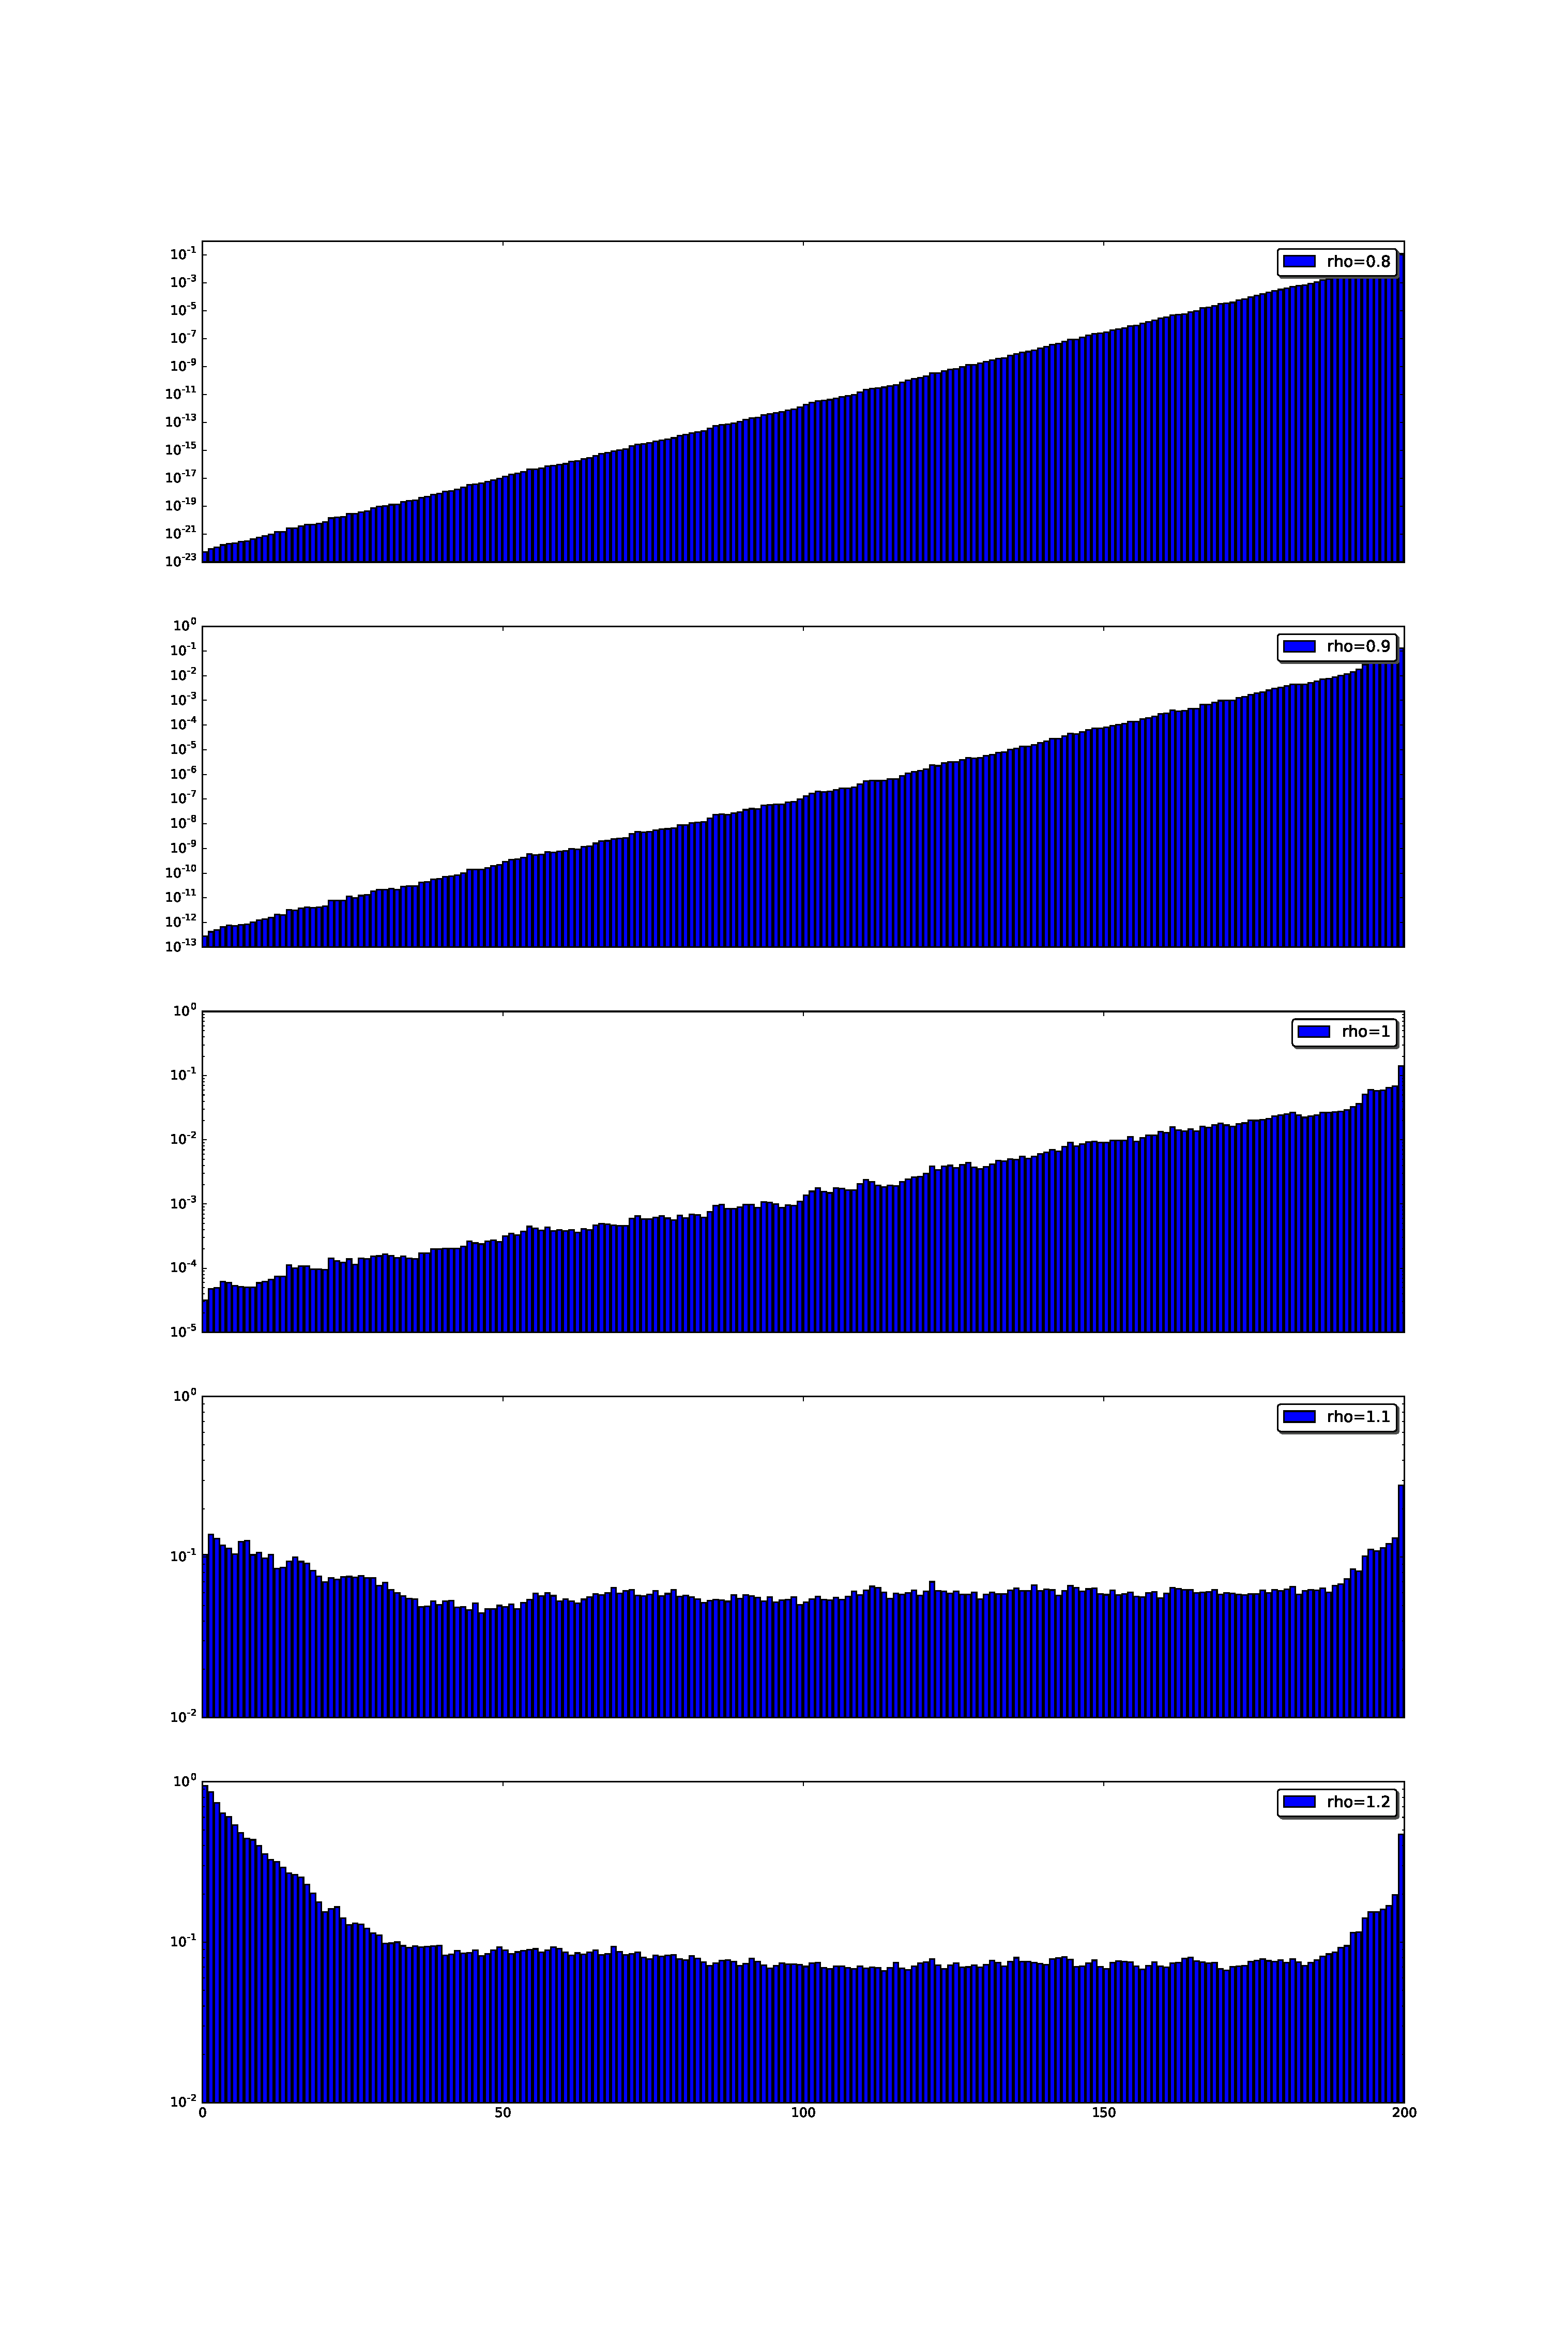
\includegraphics[width=0.9\textwidth]{chapter3/temporal_components.eps}
    \caption{Temporal components for the temporal order task varying the spectral radius of the recurrent matrix. y axis is in logarithmic scale.}
    \label{fig:temporal_norms}
\end{figure}

The first two cases, the one with spectral radius less than one, are perfect example of vanishing gradient instances: more recent temporal components have norm exponentially bigger than the more distant ones (please note that the y axis is in logarithmic scale). On the contrary such phenomenon is not observed in the cases of spectral radius bigger than one where the temporal components have roughly the same norm.

We found that, at least in the task we explored (SAY WHICH ONES), an appropriate spectral radius always allow the training process to start in a regime where the gradient does not vanish. We report some results on the effect of the initialization on the training process in chapter \ref{ch:experiments}

\section{Descent direction}

\begin{figure}
	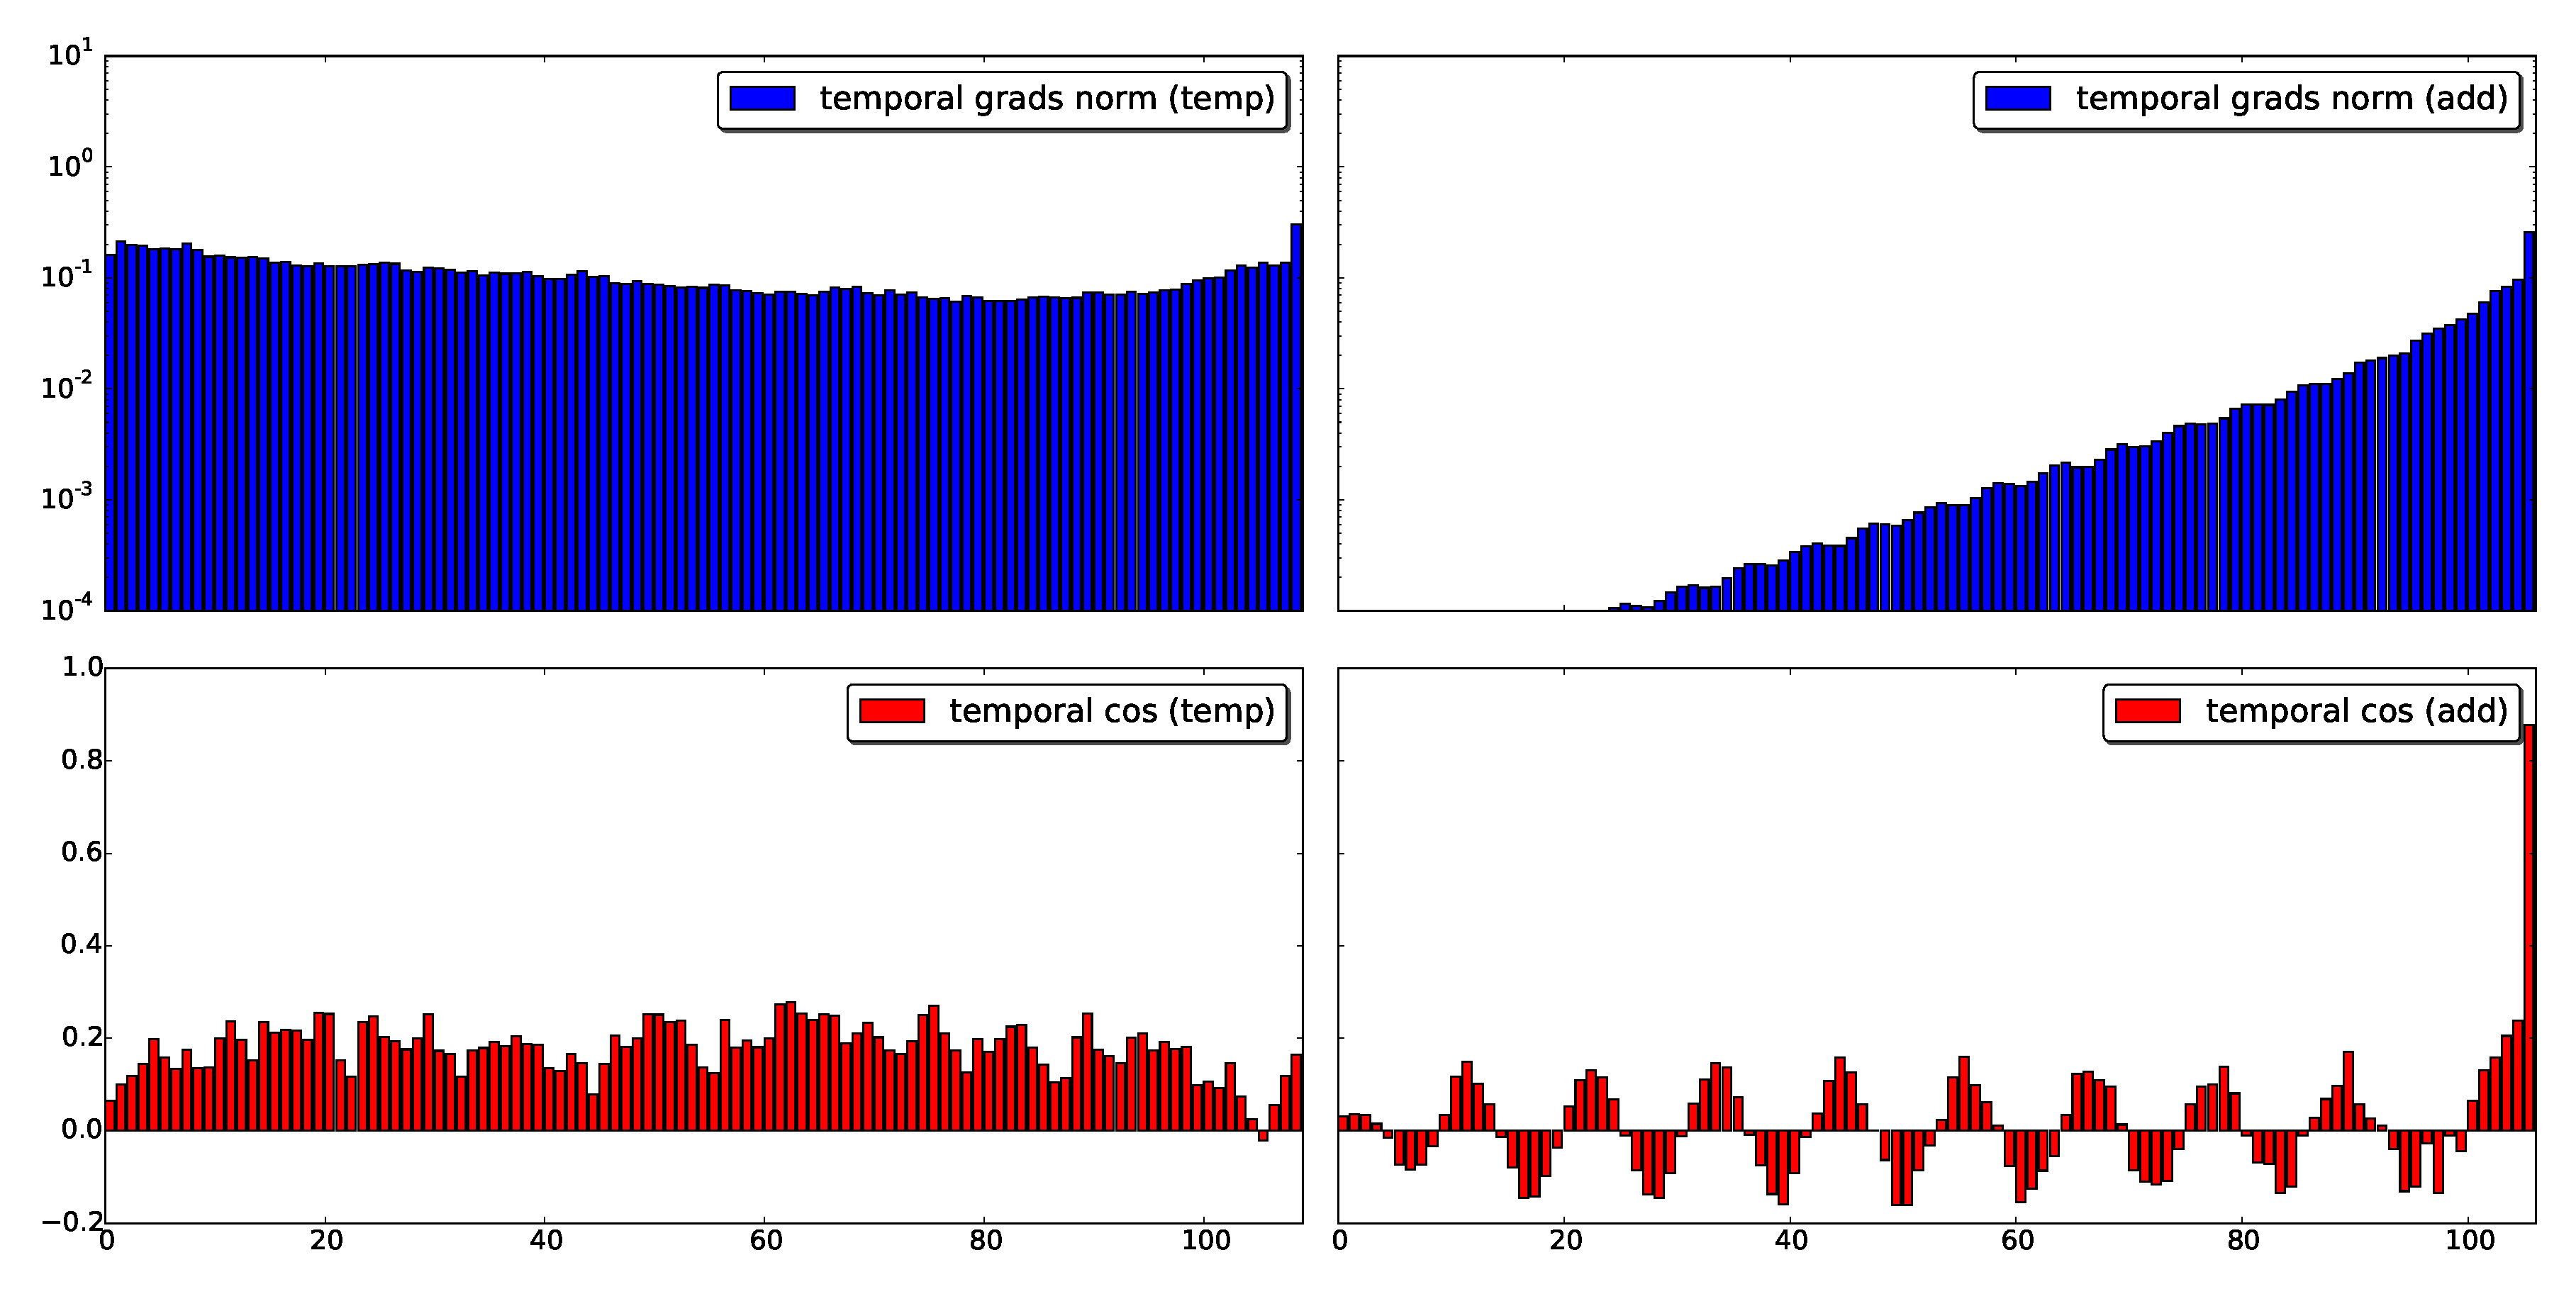
\includegraphics[width=1.4\textwidth]{chapter3/compare_add_temp_norms_1.eps}
	\caption{Temporal components for the temporal order task varying the spectral radius of the recurrent matrix. y axis is in logarithmic scale.}
	\label{fig:}
\end{figure}


The idea is to use the structure of the gradient to compute a "descent" direction which does not suffer from the vanishing problem.

\begin{itemize}
	\item normalize the temporal components:
	\begin{equation}
	g_t(\vec{x}) = \frac{\nabla L_{|t}(\vec{x})}{\norm{\nabla L_{|t}(\vec{x})}}.
	\end{equation}
	
	\item combine the normalized gradients in a simplex:
	\begin{equation}
	g(\vec{x}) = \sum_{t=1}^T \beta_t \cdot g_t(\vec{x}).
	\end{equation}
	
	with $\sum_{t=1}^T\beta_t=1, \beta_t>0$ (randomly picked at each iteration).
	\item exploit the gradient norm:
	\begin{equation}
	d(\vec{x}) = \norm{\nabla L (\vec{x})}\frac{g(\vec{x})}{\norm{g(\vec{x})}}.
	\end{equation}
\end{itemize}
\section{Learning rate}

The choice of the learning rate is crucial for the success of the training procedure. It is well known that RNNs give rise to gradients which change extremely fast in norm (the exploding gradient problem). This makes choosing a single constant step, or even designing an adaptive strategy, very difficult, at the least, for this kind of models. A simple trick which allow to choose a fixed step from the beginning is to \textit{clip the gradients}. This technique was introduced and used in slightly different forms in \cite{understandingExplodingGradients} and \cite{clippingMikolov} and we describe it in section \ref{algo:sgd}. We reformulate the version proposed in \cite{understandingExplodingGradients} as a learning rate selection strategy.
Given a direction $\vec{d}_k$ the step $\alpha_k$ is chosen as:
\begin{equation}
\alpha_k = 
\begin{cases}
	\mu  \quad &\mbox{if} \norm{\vec{d}_k}_2 \leq \tau\\
	\frac{\mu \cdot \tau}{\norm{\vec{d}_k}_2} \quad & otherwise,
\end{cases}
\end{equation}
where $\mu$ and $c$ are some positive constants. The parameter $\tau$ is the threshold on the direction norm; $\mu$ is instead the constant learning rate that is used when the norm of the direction is not above such threshold. The idea is to use a constant step when the direction has an enough small norm and vice-versa choose a step which inversely proportional when such norm is too big. We confirm, as found in works cited above, that this trick is essential to train RNNs in a stochastic framework.

\section{Putting all togheter}
TODO

\section{Proof of convergence}
 
\documentclass{article}
\usepackage[utf8]{inputenc}
\usepackage[italian]{babel}
\usepackage{graphicx}
\usepackage{cite}
\usepackage[hidelinks]{hyperref}
\usepackage{listings}
\usepackage{latexsym}
\usepackage{amsmath}
\usepackage{proof}
\usepackage{stmaryrd}
\usepackage{amssymb}
\usepackage{epstopdf}
\usepackage{pgf}
\usepackage{tikz}
\usepackage[noend]{algpseudocode}
\usepackage[ruled,noline,linesnumbered]{algorithm2e}
\usetikzlibrary{automata,arrows}
\let\emptyset\varnothing

\graphicspath{ {./images/} }

%%Notation:

%%vectors
\renewcommand{\vec}[1]{\boldsymbol{#1}}
%%sets
\newcommand{\set}[1]{\mathcal{#1}}
%%matrixes
\newcommand{\mat}[1]{#1}
%%norm
\newcommand{\norm}[1]{\left\Vert #1 \right\Vert}
%%defeq
\newcommand{\defeq}{\triangleq}
%%
\newcommand{\net}[1]{\mathrm{#1}}
%% pair<x,y>
\newcommand{\pair}[2]{\langle#1,#2\rangle}

\title{Stochastic gradient descent}
\author{Giulio Galvan}

\begin{document}
	\maketitle
\noindent
Consider the stochastic optimization problem 
\begin{equation}
	\underset{\vec{x} \in \mathbb{R}^n}{\text{min}} f(\vec{x}) = \mathbb{E[F(\vec{x}, \vec{\xi})]},
	\label{eq:stochastic_prob}
\end{equation}
where $\vec{\xi} \in \Omega \subset \mathbb{R}^d$ is a random vector.
Suppose $f(\cdot)$ is continuous, strongly convex (with constant $c$) and there exists a compact level set of $f(\cdot)$, hence (\ref{eq:stochastic_prob}) has a unique optimal solution $\vec{x}_*$. Let also $L$ be the Lipschitz constant of $\nabla f$.
We make the following two assumptions:
\begin{itemize}
	\item	It is possible to generate independent identically distributed samples of $\vec{\xi}$
	\item There exists an oracle which, for a given point $(\vec{x}, \vec{\xi})$ return a stochastic descent direction $D(\vec{x}, \vec{\xi})$ such that $d(\vec{x})\defeq\mathbb{E}[D(\vec{x}, \vec{\xi})]$ satisfies:
	\begin{equation}
	-(\vec{x}-\vec{x}_*)^T (\nabla f(\vec{x}) -g(\vec{x})) \geq -\mu L \norm{\vec{x}_j-\vec{x}_*}^2_2\quad \forall \vec{x} \in \mathbb{R}^n,
	\label{eq:angular_condition}
	\end{equation}
	for some $\mu \in (0,\frac{c}{L}) $.
\end{itemize}
Consider the algorithm defined by
\begin{equation}
	\vec{x}_{j+1} = \vec{x}_j -\gamma_j D(\vec{x}_j,\vec{\xi}_j).
	\label{eq:stochastic_algo}
\end{equation}
Each iterate $\vec{x}_j$ of such random process is a function of the history $\vec{\xi}_{[j-1]}=(\vec{\xi}_1,\dots, \vec{\xi}_{j-1})$

Let $A_j\defeq \norm{\vec{x}_j-\vec{x}_*}^2_2$ and $a_j\defeq\mathbb{E}[A_j]$.
From (\ref*{eq:stochastic_algo}) we get
\begin{equation}
\begin{aligned}
	A_{j+1} &= \frac{1}{2}\norm{\vec{x}_j - \gamma_jD(\vec{x}_j,\vec{\xi}_j) -\vec{x}_*}^2_2\\ 
	&= A_j +\frac{1}{2}\gamma_j^2\norm{D(\vec{x}_j,\vec{\xi}_j)}^2_2 - \gamma_j(\vec{x}_j-\vec{x}_*)^TD(\vec{x}_j,\vec{\xi}_j).
\end{aligned}
\label{eq:aj_rec}
\end{equation}
Since $\vec{x}_j = \vec{x}_j(\vec{\xi_{[j-1]}})$ is independent of $\vec{\xi}_j$ we have
\begin{equation}
\begin{aligned}
	\mathbb{E}_{\vec{\xi}_{[j]}}[(\vec{x}_j-\vec{x}_*)^TD(\vec{x}_j,\vec{\xi}_j)] &= \mathbb{E}_{\vec{\xi}_{[j-1]}}[\mathbb{E}_{\vec{\xi}_{[j]}}[(\vec{x}_j-\vec{x}_*)^TD(\vec{x}_j,\vec{\xi}_j)]|\vec{\xi}_{[j-1]}]\\
	&= \mathbb{E}_{\vec{\xi}_{[j-1]}}[(\vec{x}_j-\vec{x}_*)^T\mathbb{E}{\vec{\xi}_{[j]}}[D(\vec{x}_j,\vec{\xi}_j)]|\vec{\xi}_{[j-1]}]\\
	&=\mathbb{E}_{\vec{\xi}_{[j-1]}}[(\vec{x}_j-\vec{x}_*)^Td(\vec{x}_j)]\\
\end{aligned}
\label{eq:independece}
\end{equation}
Let now assume that there exists $M>0$ such that
\begin{equation}
	\mathbb{E}[\norm{D(\vec{x},\vec{\xi})}^2_2]\leq M^2 \quad \forall \vec{x} \in \mathbb{R}^n.
	\label{eq:gradient_bound}
\end{equation}
Using (\ref{eq:independece}) and (\ref{eq:gradient_bound}) we obtain, taking expectation of both sides of (\ref{eq:aj_rec})
\begin{equation}
	a_{j+1} \leq a_j - \gamma_j\mathbb{E}_{\vec{\xi}_{[j-1]}}[(\vec{x}_j-\vec{x}_*)^Td(\vec{x}_j)] + \frac{1}{2}\gamma_j^2M^2
	\label{eq:aj_rec_2}
\end{equation}
Since $f(\cdot)$ is strongly convex there exists $c>0$ such that
\begin{equation}
	(\vec{y}-\vec{x})^T(\nabla f(\vec{y})- \nabla f(\vec{x}))\geq c \norm{\vec{y}-\vec{x}}^2_2
	\label{eq:strong_convexity}
\end{equation}
By optimality of $\vec{x}_*$ we have
\begin{equation}
	(\vec{x}-\vec{x}_*)^T\nabla f(\vec{x}_*) \geq 0 \quad \vec{x} \in \mathbb{R}^n.
	\label{eq:optimality}
\end{equation}
Inequalities (\ref{eq:optimality}) and (\ref{eq:strong_convexity}) implies
\begin{equation}
	(\vec{x}-\vec{x}_*)^T \nabla f(\vec{x}) \geq c \norm{\vec{x}-\vec{x}_*}^2_2 \quad \vec{x} \in \mathbb{R}^n.
\end{equation}
Adding and subtracting the descent direction $g(\vec{x})$ we get
\begin{equation}
	(\vec{x}-\vec{x}_*)^T (\nabla f(\vec{x}) -g(\vec{x}) +g(\vec{x})) \geq c \norm{\vec{x}-\vec{x}_*}^2_2,
\end{equation}
which can be rewritten as
\begin{equation}
		(\vec{x}-\vec{x}_*)^T g(\vec{x}) \geq c \norm{\vec{x}-\vec{x}_*}^2_2 - (\vec{x}-\vec{x}_*)^T (\nabla f(\vec{x}) -g(\vec{x}))
		\label{eq:angular_inequality}
\end{equation}
From assumption (\ref{eq:angular_condition}), taking expectations of both side of (\ref{eq:angular_inequality}) we obtain
\begin{align}
\mathbb{E}[(\vec{x}_j-\vec{x}_*)^T g(\vec{x}_j)] &\geq c \mathbb{E}[\norm{\vec{x}_j-\vec{x}_*}^2_2)] - \mathbb{E}[(\vec{x}_j-\vec{x}_*)^T (\nabla f(\vec{x}_j) -g(\vec{x}_j))]\\
 &\geq c(1-\frac{\mu L}{c}) \mathbb{E}[\norm{\vec{x}_j-\vec{x}_*}^2_2)]\\
 & = 2\bar{c}a_j,
\end{align}
with $\bar{c}=c(1-\frac{\mu L}{c})$.
Hence from (\ref{eq:aj_rec_2}) follows 
\begin{equation}
	a_{j+1} \leq (1-2\bar{c}\gamma_j)a_j + \frac{1}{2}\gamma_j^2M^2.
\end{equation}
Choosing the stepsizes as $\gamma_j = \frac{\beta}{j}$ for some constant $\beta>\frac{1}{2\bar{c}}$ we get
\begin{equation}
		a_{j+1} \leq (1-2\bar{c}\gamma_j)a_j + \frac{1}{2}\frac{\beta^2M^2}{j^2}.
\end{equation}
It follows by induction that
\begin{equation}
	\mathbb{E}[\norm{\vec{x}_j - \vec{x}_*}^2_2] = 2a_j\leq \frac{Q(\beta)}{j},
\end{equation}
where 
\begin{equation}
	Q(\beta) = max\left\{\frac{\beta^2M^2}{2\bar{c}-1},\norm{\vec{x}_1 - \vec{x}_*}^2_2 \right\}.
\end{equation}
Hence, since
\begin{equation}
	f(\vec{x})\leq f(\vec{x}_*) + \frac{1}{2}L\norm{\vec{x} - \vec{x}_*}^2_2, \quad \forall \vec{x} \in \mathbb{R}^n,
\end{equation}
we obtain
\begin{equation}
	\mathbb{E}[f(\vec{x}_j)-f(\vec{x}_*)] \leq \frac{1}{2} L \mathbb{E}[\norm{\vec{x}_j - \vec{x}_*}^2_2] \leq \frac{1}{2}LQ(\beta)
\end{equation}

\paragraph{Sufficient descent direction condition} Assumption \ref{eq:angular_condition} can be further elaborated.
Let $\theta$ be the angle between $\nabla f(\vec{x})$ and $g(\vec{x})$ and $\norm{g(\vec{x})} = \alpha \norm{\nabla f(\vec{x})}$ for some $\alpha>0$.
Then,
\begin{align}
	\norm{\nabla f(\vec{x}_j)-g(\vec{x}_j)}^2 &= \norm{\nabla f(\vec{x}_j)}^2 + \norm{g(\vec{x}_j)}^2 -2\norm{\nabla f(\vec{x}_j)}\norm{g(\vec{x}_j)}\cos\theta_j\\
	&=  \norm{\nabla f(\vec{x}_j)}^2(1+\alpha_j^2-2\alpha_j \cos\theta_j).
\end{align}
Since $\nabla f(\vec{x}_*)=0$, using Lipschitz continuity of $\nabla f$ (with constant L) we get
\begin{equation}
	\norm{\nabla f(\vec{x}_j)-g(\vec{x})} \leq L\norm{\vec{x}-\vec{x}_*} (1+\alpha^2-2\alpha \cos\theta)^{\frac{1}{2}}
\end{equation}
Hence
\begin{align}
(\vec{x}-\vec{x}_*)^T (\nabla f(\vec{x}) -g(\vec{x})) &\leq \norm{\vec{x}-\vec{x}_*} \norm{\nabla f(\vec{x}) -g(\vec{x})}\\
&\leq L\norm{\vec{x}-\vec{x}_*}^2 (1+\alpha^2-2\alpha \cos\theta)^{\frac{1}{2}}.
\end{align}
Hence a sufficient condition for assumption \ref{eq:angular_condition} to hold is
\begin{equation}
	1+\alpha^2-2\alpha \cos\theta_j\leq \mu^2
\end{equation}

\end{document}      




\chapter{Experiments}
  \label{ch:experiments}
  \section{Experiments on synthetic datasets}
In this section we report some experiments which highlights the effects of the proposed techniques on the training process. In all the experiments with artificial dataset we employed a potentially infinite training-set, since we generate data on the fly. We used a validation set to determine the success of the training process. We define a training run to be successful if the error on the validation set if less than 1\%. The error is clearly defined for each task, see appendix \ref{app:tasks} for more details on the tasks. The validation test is composed by $10^4$ examples of different lengths sampled once at the beginning. In all the experiments we used a learning rate of $10^{-3}$, clipping threshold of $1$, batch-size equal to $100$. We did not experiment much on the batch size. We found instead that the this combination of learning rate and threshold is generally good for all the task and lengths, although for tasks with smaller sequences more aggressive learning rate can be used.

\subsection{The effect of the spectral initialization}

For this experiment we consider the temporal order task which has always been considered effectively impossible to solve using the a plain version of the stochastic  gradient descent algorithm.
In \cite{advancesInOptimizingRnns}, for instance, are reported the rate of success of SGD and SGD modified with gradient clipping technique for such task with different input lengths. It shows that for sequences longer than 20 neither one of the algorithms can solve the problem. We repeated the same experiment, namely training the network varying the length\footnote{Here we refer as the length of the task to the minim length of the input sequences} of the input sequences, with the SGD algorithm modified with the gradient clipping technique using our initialization scheme. 
%In figure \ref{fig:spectral_init_effect} are shown the number of iterations (means of 5 different runs with different random seeds) required to solve the problem for lengths in [50 100 150 200]. The important thing to notice is that, contrarily to what commonly believed, it is possible to train RNNs with SGD (with gradient clipping): not one of the runs for any length failed.

In Figure \ref{fig:temporal_rates} we compare the rate of success for different initialization schemes, namely a standard gaussian initialization, and the initialization scheme we propose, i.e. scaling $\mat{W}_{rec}$ to have spectral radius bigger than one. We can notice that scaling the recurrent matrix has a huge effect on the rate of convergence: where the standard scheme fails for sequences longer than 20, with the spectral initialization we manage to succeed up to sequence of length 150.


\begin{figure}
	\centering
	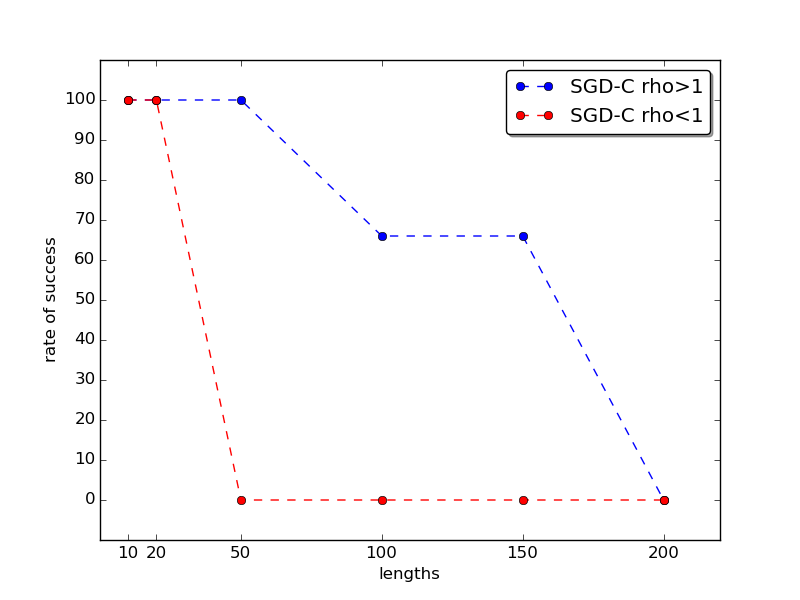
\includegraphics[width= 0.9\textwidth]{chapter4/temporal_rates.png}
	\caption{Rate of success (mean of 5 runs) for the temporal order task for various lengths with SGD modified with gradient clipping. In blue and red the results when $W_rec$ is initialized with spectral radius bigger and smaller than one respectively}
	\label{fig:temporal_rates}
\end{figure}

%\begin{figure}
%	\centering
%	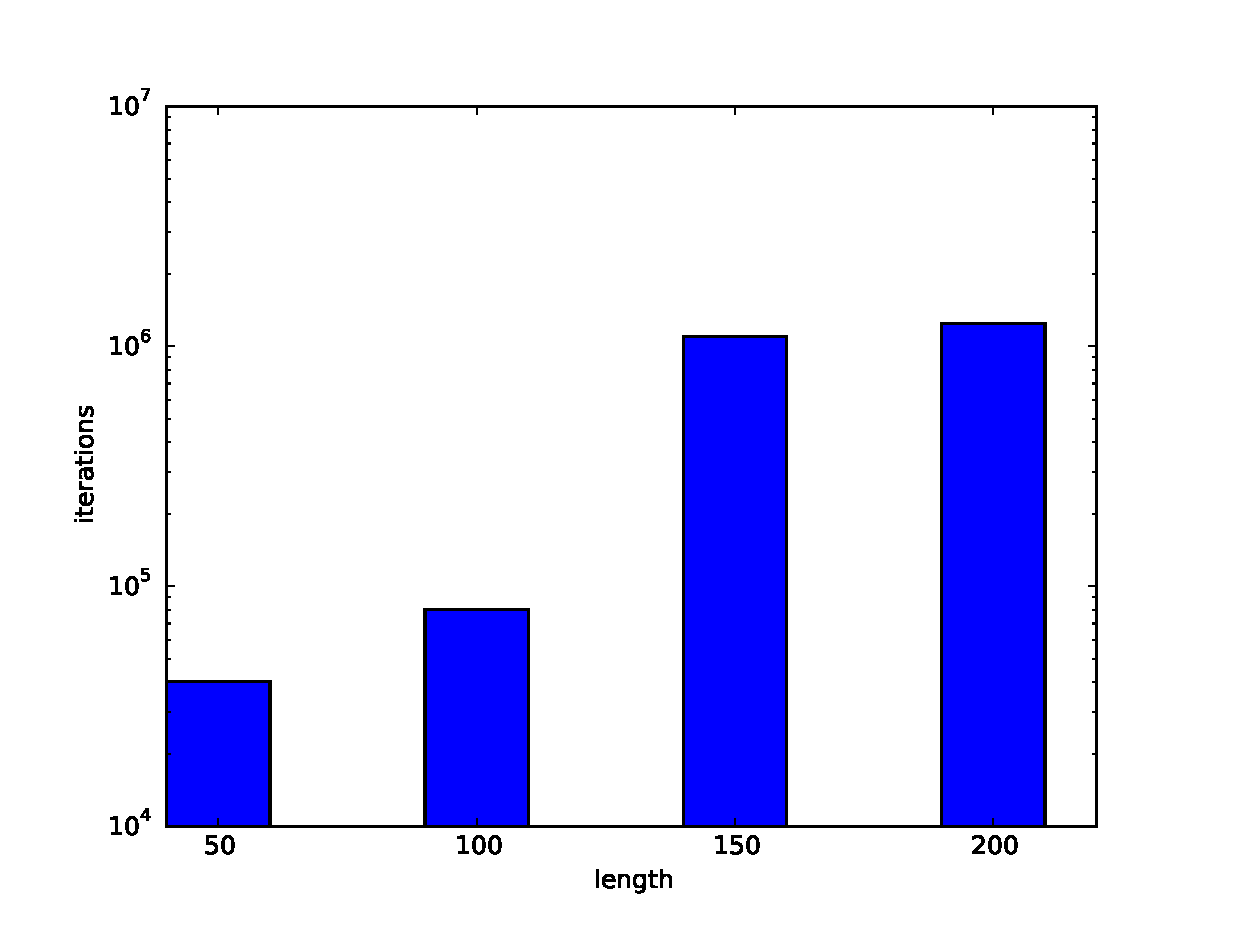
\includegraphics[width= 0.9\textwidth]{chapter4/spectral_init_exp.eps}
%	\caption{Number of iterations (means of 5 different random seed) needed to solve the task for different lengths}
%	\label{fig:spectral_init_effect}
%\end{figure}


\subsection{The effect of using the simplex direction}
The first experiment we ran is developed to compare the simplex strategy and the variant with the conditional switching to the anti-gradient with the standard SGD. We tested the three algorithms on the addition problem (T=100). In Figure \ref{fig:comparisong_add_simplex} is shown the loss on the validation set during the training process (until convergence). Aside from the obvious consideration that the conditioned simplex strategy converges first, and the anti-gradient for last, we can notice that the simplex direction is particularly beneficial in the first part of the training process, which is when the effect of the vanishing gradient is more evident. This confirms that the simplex direction helps when dealing with vanishing gradients. Moreover the idea to switch back to the anti-gradient when the gradient has a sufficiently high norm seems to be effective.

\begin{figure}
	\centering
	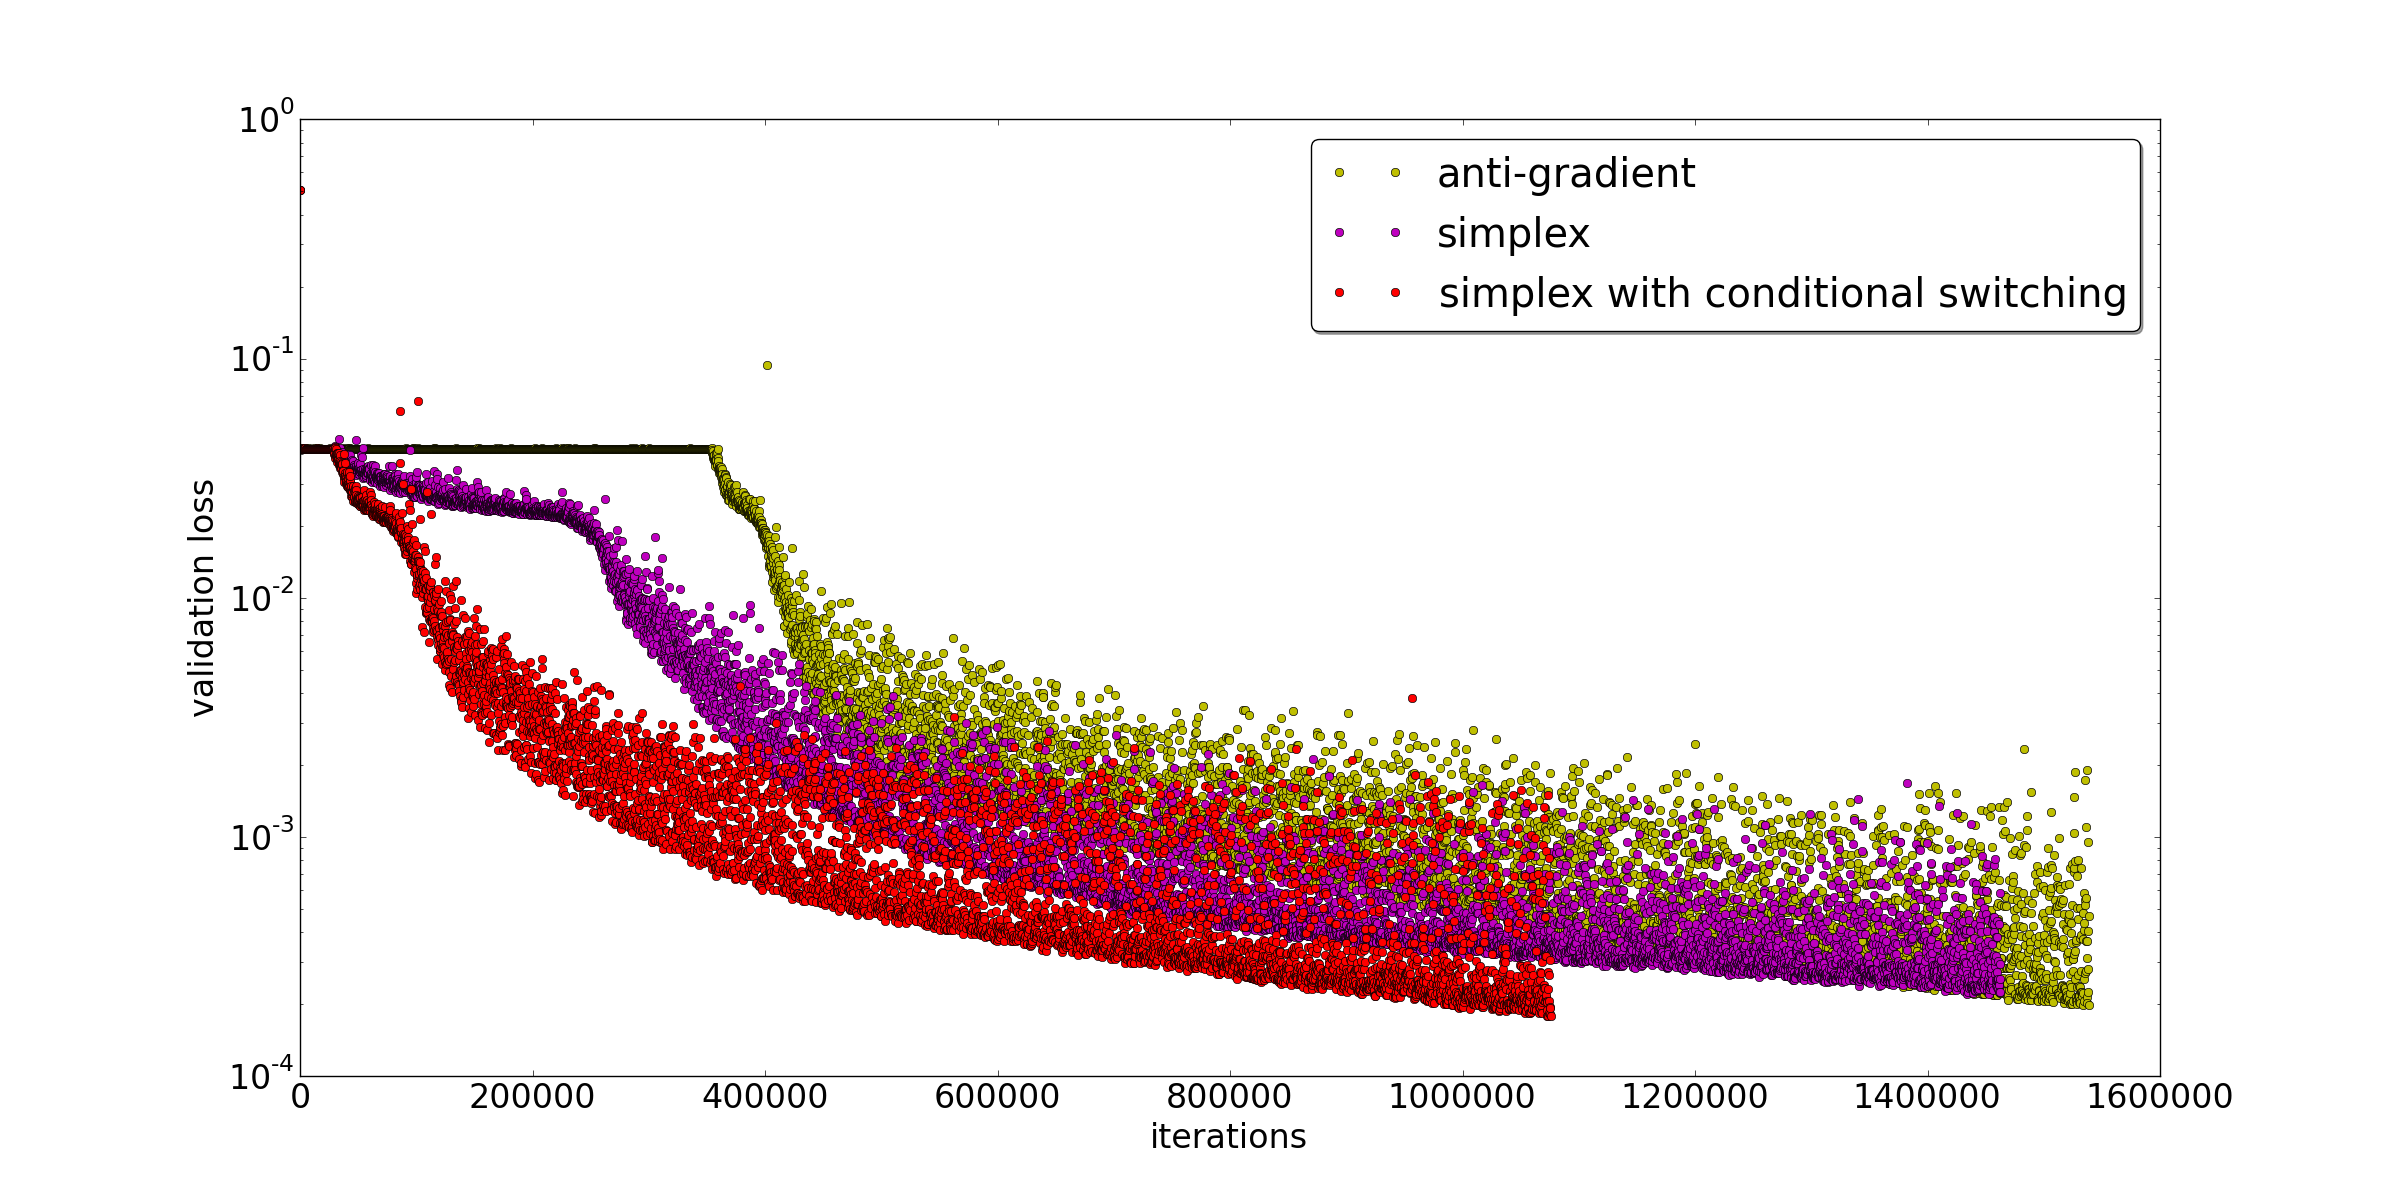
\includegraphics[width= 0.8\textwidth]{chapter4/compare_add_simplex.png}
	\caption{Comparison between SGD using a descent direction the anti-gradient, the simplex direction and the simplex direction conditioned for the addition task (T=100). In y axis the loss (mean squared error) in logarithmic scale.}
	\label{fig:comparisong_add_simplex}
\end{figure}

In Table \ref{table:add_100_comparison_iterations} are shown the number of iterations (mean values of 5 runs) needed for convergence for each strategy. Note that, although in the table are reported for simplicity only the mean values, each run follows the trend of Figure \ref{fig:comparisong_add_simplex}.
\begin{table}
	\centering
	\begin{tabular}{C{2cm} | C{2cm} | C{4cm}}
		anti-gradient & simplex & simplex with conditional switching \\
		1807466 & 2338500 & 1332866 \\
	\end{tabular}
	\caption{Number of iterations until convergence for the addition task (T=100). Mean of 5 runs. TODO UPDATE RESULTS WITH NEW RUNS}
	\label{table:add_100_comparison_iterations}
\end{table}

We repeated the experiment also for the temporal order task and ... ADD RESULTS WHEN READY 
   
\section{Polyphonic music prediction}

In this experiment we considered the task of polyphonic music prediction. The input sequences are polyphonic songs and the aim is, at each time step, to predict which notes are played next. More precisely the input sequences are obtained from a piano roll of MIDI files where each time step corresponds to a beat (usually a quarter or an octave): each step of the sequence is hence composed of $d$, the number of notes that can be played,  binary elements which specify if the correspondent note is played or not at the current beat.

We use as a reference the work done in \cite{BoulangerMuse} which compares several different approaches, RNNs amongst them. We use the dataset \textsl{MuseData} made available by the authors on their website
\url{http://www-etud.iro.umontreal.ca/~boulanni/icml2012}, using the provided split in train, set and validation sets.

The RNN architecture we employed is a standard RNN with \textit{tanh} units, 88 input and output units (the total number of notes from A0 to C8). We use as output function the logistic function

\begin{equation}
	F(x)=\frac{1}{1+e^{-x}};
\end{equation}
in this way we can interpret the value of each output unit as the probability that such note is played. We used the cross-entropy as loss function for each time step, hence, the loss for the whole sequence is given by:

\begin{equation}
	L(\vec{y}) = \frac{1}{T}\sum_{t=1}^{T}\sum_{i=1}^{d} \bar{y}_i \log(y_i) + (1-\bar{y}_i)\log(1-y_i)
\end{equation}

An important difference with the artificial tasks considered before is that in this case the loss is not computed only on the last step, hence the training does not suffer from the vanishing problem. ADD SOME JUSTIFICATION

We trained the network with stochastic gradient descent with $lr=0.001$. We clipped the gradient at $3$. We explored different number of hidden units, namely 50, 100, 200, 300.

Figure \ref{fig:overfitting_muse} shows the loss function computed on both train and validation sets during the training for model with different hidden units. The most obvious observation is that at a certain point the training procedure starts to over-fit and that model with more hidden units start to over-fit sooner.

\begin{figure}
	\centering
\resizebox{13cm}{!}{
	%% Creator: Matplotlib, PGF backend
%%
%% To include the figure in your LaTeX document, write
%%   \input{<filename>.pgf}
%%
%% Make sure the required packages are loaded in your preamble
%%   \usepackage{pgf}
%%
%% Figures using additional raster images can only be included by \input if
%% they are in the same directory as the main LaTeX file. For loading figures
%% from other directories you can use the `import` package
%%   \usepackage{import}
%% and then include the figures with
%%   \import{<path to file>}{<filename>.pgf}
%%
%% Matplotlib used the following preamble
%%   \usepackage{fontspec}
%%   \setmainfont{DejaVu Serif}
%%   \setsansfont{DejaVu Sans}
%%   \setmonofont{DejaVu Sans Mono}
%%
\begingroup%
\makeatletter%
\begin{pgfpicture}%
\pgfpathrectangle{\pgfpointorigin}{\pgfqpoint{8.000000in}{6.000000in}}%
\pgfusepath{use as bounding box, clip}%
\begin{pgfscope}%
\pgfsetbuttcap%
\pgfsetmiterjoin%
\pgfsetlinewidth{0.000000pt}%
\definecolor{currentstroke}{rgb}{0.000000,0.000000,0.000000}%
\pgfsetstrokecolor{currentstroke}%
\pgfsetstrokeopacity{0.000000}%
\pgfsetdash{}{0pt}%
\pgfpathmoveto{\pgfqpoint{0.000000in}{0.000000in}}%
\pgfpathlineto{\pgfqpoint{8.000000in}{0.000000in}}%
\pgfpathlineto{\pgfqpoint{8.000000in}{6.000000in}}%
\pgfpathlineto{\pgfqpoint{0.000000in}{6.000000in}}%
\pgfpathclose%
\pgfusepath{}%
\end{pgfscope}%
\begin{pgfscope}%
\pgfsetbuttcap%
\pgfsetmiterjoin%
\pgfsetlinewidth{0.000000pt}%
\definecolor{currentstroke}{rgb}{0.000000,0.000000,0.000000}%
\pgfsetstrokecolor{currentstroke}%
\pgfsetstrokeopacity{0.000000}%
\pgfsetdash{}{0pt}%
\pgfpathmoveto{\pgfqpoint{1.000000in}{0.600000in}}%
\pgfpathlineto{\pgfqpoint{7.200000in}{0.600000in}}%
\pgfpathlineto{\pgfqpoint{7.200000in}{5.400000in}}%
\pgfpathlineto{\pgfqpoint{1.000000in}{5.400000in}}%
\pgfpathclose%
\pgfusepath{}%
\end{pgfscope}%
\begin{pgfscope}%
\pgfpathrectangle{\pgfqpoint{1.000000in}{0.600000in}}{\pgfqpoint{6.200000in}{4.800000in}} %
\pgfusepath{clip}%
\pgfsetbuttcap%
\pgfsetroundjoin%
\pgfsetlinewidth{5.018750pt}%
\definecolor{currentstroke}{rgb}{0.750000,0.750000,0.000000}%
\pgfsetstrokecolor{currentstroke}%
\pgfsetdash{{6.000000pt}{6.000000pt}}{0.000000pt}%
\pgfpathmoveto{\pgfqpoint{1.000000in}{11.707884in}}%
\pgfpathmoveto{\pgfqpoint{1.053550in}{5.410000in}}%
\pgfpathlineto{\pgfqpoint{1.062000in}{4.416161in}}%
\pgfpathlineto{\pgfqpoint{1.124000in}{4.060909in}}%
\pgfpathlineto{\pgfqpoint{1.186000in}{3.835789in}}%
\pgfpathlineto{\pgfqpoint{1.248000in}{3.653026in}}%
\pgfpathlineto{\pgfqpoint{1.310000in}{3.540007in}}%
\pgfpathlineto{\pgfqpoint{1.372000in}{3.460733in}}%
\pgfpathlineto{\pgfqpoint{1.434000in}{3.403667in}}%
\pgfpathlineto{\pgfqpoint{1.496000in}{3.359651in}}%
\pgfpathlineto{\pgfqpoint{1.558000in}{3.325708in}}%
\pgfpathlineto{\pgfqpoint{1.620000in}{3.293706in}}%
\pgfpathlineto{\pgfqpoint{1.682000in}{3.276136in}}%
\pgfpathlineto{\pgfqpoint{1.744000in}{3.274559in}}%
\pgfpathlineto{\pgfqpoint{1.806000in}{3.243188in}}%
\pgfpathlineto{\pgfqpoint{1.868000in}{3.224138in}}%
\pgfpathlineto{\pgfqpoint{1.930000in}{3.212762in}}%
\pgfpathlineto{\pgfqpoint{1.992000in}{3.213874in}}%
\pgfpathlineto{\pgfqpoint{2.054000in}{3.197465in}}%
\pgfpathlineto{\pgfqpoint{2.116000in}{3.202803in}}%
\pgfpathlineto{\pgfqpoint{2.178000in}{3.184925in}}%
\pgfpathlineto{\pgfqpoint{2.240000in}{3.177163in}}%
\pgfpathlineto{\pgfqpoint{2.302000in}{3.167207in}}%
\pgfpathlineto{\pgfqpoint{2.364000in}{3.162144in}}%
\pgfpathlineto{\pgfqpoint{2.426000in}{3.159992in}}%
\pgfpathlineto{\pgfqpoint{2.488000in}{3.156644in}}%
\pgfpathlineto{\pgfqpoint{2.550000in}{3.153872in}}%
\pgfpathlineto{\pgfqpoint{2.612000in}{3.140220in}}%
\pgfpathlineto{\pgfqpoint{2.674000in}{3.135862in}}%
\pgfpathlineto{\pgfqpoint{2.736000in}{3.132202in}}%
\pgfpathlineto{\pgfqpoint{2.798000in}{3.125717in}}%
\pgfpathlineto{\pgfqpoint{2.860000in}{3.120963in}}%
\pgfpathlineto{\pgfqpoint{2.922000in}{3.117330in}}%
\pgfpathlineto{\pgfqpoint{2.984000in}{3.125500in}}%
\pgfpathlineto{\pgfqpoint{3.046000in}{3.104851in}}%
\pgfpathlineto{\pgfqpoint{3.108000in}{3.081228in}}%
\pgfpathlineto{\pgfqpoint{3.170000in}{3.053355in}}%
\pgfpathlineto{\pgfqpoint{3.232000in}{3.029147in}}%
\pgfpathlineto{\pgfqpoint{3.294000in}{3.011202in}}%
\pgfpathlineto{\pgfqpoint{3.356000in}{2.983134in}}%
\pgfpathlineto{\pgfqpoint{3.418000in}{2.967518in}}%
\pgfpathlineto{\pgfqpoint{3.480000in}{2.955161in}}%
\pgfpathlineto{\pgfqpoint{3.542000in}{2.940812in}}%
\pgfpathlineto{\pgfqpoint{3.604000in}{2.928221in}}%
\pgfpathlineto{\pgfqpoint{3.666000in}{2.920379in}}%
\pgfpathlineto{\pgfqpoint{3.728000in}{2.913966in}}%
\pgfpathlineto{\pgfqpoint{3.790000in}{2.906405in}}%
\pgfpathlineto{\pgfqpoint{3.852000in}{2.896223in}}%
\pgfpathlineto{\pgfqpoint{3.914000in}{2.895969in}}%
\pgfpathlineto{\pgfqpoint{3.976000in}{2.887995in}}%
\pgfpathlineto{\pgfqpoint{4.038000in}{2.883037in}}%
\pgfpathlineto{\pgfqpoint{4.100000in}{2.884406in}}%
\pgfpathlineto{\pgfqpoint{4.162000in}{2.874045in}}%
\pgfpathlineto{\pgfqpoint{4.224000in}{2.872588in}}%
\pgfpathlineto{\pgfqpoint{4.286000in}{2.870521in}}%
\pgfpathlineto{\pgfqpoint{4.348000in}{2.861050in}}%
\pgfpathlineto{\pgfqpoint{4.410000in}{2.858250in}}%
\pgfpathlineto{\pgfqpoint{4.472000in}{2.854658in}}%
\pgfpathlineto{\pgfqpoint{4.534000in}{2.850677in}}%
\pgfpathlineto{\pgfqpoint{4.596000in}{2.852461in}}%
\pgfpathlineto{\pgfqpoint{4.658000in}{2.844414in}}%
\pgfpathlineto{\pgfqpoint{4.720000in}{2.838670in}}%
\pgfpathlineto{\pgfqpoint{4.782000in}{2.835017in}}%
\pgfpathlineto{\pgfqpoint{4.844000in}{2.831825in}}%
\pgfpathlineto{\pgfqpoint{4.906000in}{2.827759in}}%
\pgfpathlineto{\pgfqpoint{4.968000in}{2.824420in}}%
\pgfpathlineto{\pgfqpoint{5.030000in}{2.825957in}}%
\pgfpathlineto{\pgfqpoint{5.092000in}{2.826489in}}%
\pgfpathlineto{\pgfqpoint{5.154000in}{2.824234in}}%
\pgfpathlineto{\pgfqpoint{5.216000in}{2.814304in}}%
\pgfpathlineto{\pgfqpoint{5.278000in}{2.816478in}}%
\pgfpathlineto{\pgfqpoint{5.340000in}{2.809480in}}%
\pgfpathlineto{\pgfqpoint{5.402000in}{2.806646in}}%
\pgfpathlineto{\pgfqpoint{5.464000in}{2.807829in}}%
\pgfpathlineto{\pgfqpoint{5.526000in}{2.803266in}}%
\pgfpathlineto{\pgfqpoint{5.588000in}{2.801938in}}%
\pgfpathlineto{\pgfqpoint{5.650000in}{2.804153in}}%
\pgfpathlineto{\pgfqpoint{5.712000in}{2.798371in}}%
\pgfpathlineto{\pgfqpoint{5.774000in}{2.795959in}}%
\pgfpathlineto{\pgfqpoint{5.836000in}{2.795911in}}%
\pgfpathlineto{\pgfqpoint{5.898000in}{2.792581in}}%
\pgfpathlineto{\pgfqpoint{5.960000in}{2.787332in}}%
\pgfpathlineto{\pgfqpoint{6.022000in}{2.780784in}}%
\pgfpathlineto{\pgfqpoint{6.084000in}{2.779299in}}%
\pgfpathlineto{\pgfqpoint{6.146000in}{2.785930in}}%
\pgfpathlineto{\pgfqpoint{6.208000in}{2.777130in}}%
\pgfpathlineto{\pgfqpoint{6.270000in}{2.778849in}}%
\pgfpathlineto{\pgfqpoint{6.332000in}{2.779990in}}%
\pgfpathlineto{\pgfqpoint{6.394000in}{2.778659in}}%
\pgfpathlineto{\pgfqpoint{6.456000in}{2.766695in}}%
\pgfpathlineto{\pgfqpoint{6.518000in}{2.777405in}}%
\pgfpathlineto{\pgfqpoint{6.580000in}{2.765987in}}%
\pgfpathlineto{\pgfqpoint{6.642000in}{2.760919in}}%
\pgfpathlineto{\pgfqpoint{6.704000in}{2.770963in}}%
\pgfpathlineto{\pgfqpoint{6.766000in}{2.758633in}}%
\pgfpathlineto{\pgfqpoint{6.828000in}{2.758506in}}%
\pgfpathlineto{\pgfqpoint{6.890000in}{2.761158in}}%
\pgfpathlineto{\pgfqpoint{6.952000in}{2.753991in}}%
\pgfpathlineto{\pgfqpoint{7.014000in}{2.749411in}}%
\pgfpathlineto{\pgfqpoint{7.076000in}{2.752292in}}%
\pgfpathlineto{\pgfqpoint{7.138000in}{2.759344in}}%
\pgfpathlineto{\pgfqpoint{7.200000in}{2.751716in}}%
\pgfpathlineto{\pgfqpoint{7.210000in}{2.750475in}}%
\pgfusepath{stroke}%
\end{pgfscope}%
\begin{pgfscope}%
\pgfpathrectangle{\pgfqpoint{1.000000in}{0.600000in}}{\pgfqpoint{6.200000in}{4.800000in}} %
\pgfusepath{clip}%
\pgfsetrectcap%
\pgfsetroundjoin%
\pgfsetlinewidth{1.505625pt}%
\definecolor{currentstroke}{rgb}{0.750000,0.750000,0.000000}%
\pgfsetstrokecolor{currentstroke}%
\pgfsetdash{}{0pt}%
\pgfpathmoveto{\pgfqpoint{1.001897in}{5.410000in}}%
\pgfpathlineto{\pgfqpoint{1.002067in}{4.847990in}}%
\pgfpathlineto{\pgfqpoint{1.004133in}{4.582446in}}%
\pgfpathlineto{\pgfqpoint{1.006200in}{4.538903in}}%
\pgfpathlineto{\pgfqpoint{1.010333in}{4.509359in}}%
\pgfpathlineto{\pgfqpoint{1.016533in}{4.490692in}}%
\pgfpathlineto{\pgfqpoint{1.022733in}{4.469953in}}%
\pgfpathlineto{\pgfqpoint{1.028933in}{4.440898in}}%
\pgfpathlineto{\pgfqpoint{1.035133in}{4.399943in}}%
\pgfpathlineto{\pgfqpoint{1.049600in}{4.293409in}}%
\pgfpathlineto{\pgfqpoint{1.053733in}{4.271271in}}%
\pgfpathlineto{\pgfqpoint{1.074400in}{4.148825in}}%
\pgfpathlineto{\pgfqpoint{1.086800in}{4.051486in}}%
\pgfpathlineto{\pgfqpoint{1.095067in}{4.005683in}}%
\pgfpathlineto{\pgfqpoint{1.111600in}{3.936813in}}%
\pgfpathlineto{\pgfqpoint{1.113667in}{3.931831in}}%
\pgfpathlineto{\pgfqpoint{1.119867in}{3.905846in}}%
\pgfpathlineto{\pgfqpoint{1.138467in}{3.828948in}}%
\pgfpathlineto{\pgfqpoint{1.150867in}{3.775807in}}%
\pgfpathlineto{\pgfqpoint{1.179800in}{3.675714in}}%
\pgfpathlineto{\pgfqpoint{1.214933in}{3.562134in}}%
\pgfpathlineto{\pgfqpoint{1.217000in}{3.557606in}}%
\pgfpathlineto{\pgfqpoint{1.225267in}{3.530115in}}%
\pgfpathlineto{\pgfqpoint{1.227333in}{3.527813in}}%
\pgfpathlineto{\pgfqpoint{1.233533in}{3.507362in}}%
\pgfpathlineto{\pgfqpoint{1.248000in}{3.469484in}}%
\pgfpathlineto{\pgfqpoint{1.252133in}{3.463937in}}%
\pgfpathlineto{\pgfqpoint{1.254200in}{3.454014in}}%
\pgfpathlineto{\pgfqpoint{1.256267in}{3.451280in}}%
\pgfpathlineto{\pgfqpoint{1.258333in}{3.444609in}}%
\pgfpathlineto{\pgfqpoint{1.260400in}{3.442082in}}%
\pgfpathlineto{\pgfqpoint{1.264533in}{3.433219in}}%
\pgfpathlineto{\pgfqpoint{1.266600in}{3.430027in}}%
\pgfpathlineto{\pgfqpoint{1.268667in}{3.424772in}}%
\pgfpathlineto{\pgfqpoint{1.270733in}{3.422616in}}%
\pgfpathlineto{\pgfqpoint{1.274867in}{3.411449in}}%
\pgfpathlineto{\pgfqpoint{1.279000in}{3.405560in}}%
\pgfpathlineto{\pgfqpoint{1.283133in}{3.397458in}}%
\pgfpathlineto{\pgfqpoint{1.287267in}{3.390877in}}%
\pgfpathlineto{\pgfqpoint{1.299667in}{3.370867in}}%
\pgfpathlineto{\pgfqpoint{1.301733in}{3.368726in}}%
\pgfpathlineto{\pgfqpoint{1.305867in}{3.361516in}}%
\pgfpathlineto{\pgfqpoint{1.307933in}{3.357361in}}%
\pgfpathlineto{\pgfqpoint{1.310000in}{3.357242in}}%
\pgfpathlineto{\pgfqpoint{1.314133in}{3.348164in}}%
\pgfpathlineto{\pgfqpoint{1.316200in}{3.345382in}}%
\pgfpathlineto{\pgfqpoint{1.318267in}{3.347104in}}%
\pgfpathlineto{\pgfqpoint{1.320333in}{3.341166in}}%
\pgfpathlineto{\pgfqpoint{1.322400in}{3.343087in}}%
\pgfpathlineto{\pgfqpoint{1.324467in}{3.333439in}}%
\pgfpathlineto{\pgfqpoint{1.326533in}{3.332963in}}%
\pgfpathlineto{\pgfqpoint{1.332733in}{3.322823in}}%
\pgfpathlineto{\pgfqpoint{1.341000in}{3.311183in}}%
\pgfpathlineto{\pgfqpoint{1.343067in}{3.309629in}}%
\pgfpathlineto{\pgfqpoint{1.347200in}{3.304005in}}%
\pgfpathlineto{\pgfqpoint{1.349267in}{3.302120in}}%
\pgfpathlineto{\pgfqpoint{1.351333in}{3.303174in}}%
\pgfpathlineto{\pgfqpoint{1.353400in}{3.295160in}}%
\pgfpathlineto{\pgfqpoint{1.355467in}{3.295115in}}%
\pgfpathlineto{\pgfqpoint{1.357533in}{3.291465in}}%
\pgfpathlineto{\pgfqpoint{1.359600in}{3.291793in}}%
\pgfpathlineto{\pgfqpoint{1.361667in}{3.285574in}}%
\pgfpathlineto{\pgfqpoint{1.363733in}{3.288652in}}%
\pgfpathlineto{\pgfqpoint{1.367867in}{3.278347in}}%
\pgfpathlineto{\pgfqpoint{1.369933in}{3.278527in}}%
\pgfpathlineto{\pgfqpoint{1.376133in}{3.269288in}}%
\pgfpathlineto{\pgfqpoint{1.378200in}{3.269955in}}%
\pgfpathlineto{\pgfqpoint{1.380267in}{3.265544in}}%
\pgfpathlineto{\pgfqpoint{1.382333in}{3.265240in}}%
\pgfpathlineto{\pgfqpoint{1.384400in}{3.263596in}}%
\pgfpathlineto{\pgfqpoint{1.390600in}{3.254961in}}%
\pgfpathlineto{\pgfqpoint{1.392667in}{3.255016in}}%
\pgfpathlineto{\pgfqpoint{1.394733in}{3.251129in}}%
\pgfpathlineto{\pgfqpoint{1.396800in}{3.251456in}}%
\pgfpathlineto{\pgfqpoint{1.400933in}{3.247098in}}%
\pgfpathlineto{\pgfqpoint{1.405067in}{3.243893in}}%
\pgfpathlineto{\pgfqpoint{1.407133in}{3.239480in}}%
\pgfpathlineto{\pgfqpoint{1.409200in}{3.241321in}}%
\pgfpathlineto{\pgfqpoint{1.411267in}{3.236282in}}%
\pgfpathlineto{\pgfqpoint{1.413333in}{3.235775in}}%
\pgfpathlineto{\pgfqpoint{1.415400in}{3.231935in}}%
\pgfpathlineto{\pgfqpoint{1.421600in}{3.230449in}}%
\pgfpathlineto{\pgfqpoint{1.423667in}{3.224789in}}%
\pgfpathlineto{\pgfqpoint{1.425733in}{3.224100in}}%
\pgfpathlineto{\pgfqpoint{1.429867in}{3.219989in}}%
\pgfpathlineto{\pgfqpoint{1.434000in}{3.218326in}}%
\pgfpathlineto{\pgfqpoint{1.436067in}{3.215855in}}%
\pgfpathlineto{\pgfqpoint{1.438133in}{3.218790in}}%
\pgfpathlineto{\pgfqpoint{1.442267in}{3.210462in}}%
\pgfpathlineto{\pgfqpoint{1.444333in}{3.211607in}}%
\pgfpathlineto{\pgfqpoint{1.446400in}{3.209953in}}%
\pgfpathlineto{\pgfqpoint{1.448467in}{3.211322in}}%
\pgfpathlineto{\pgfqpoint{1.450533in}{3.204141in}}%
\pgfpathlineto{\pgfqpoint{1.454667in}{3.199963in}}%
\pgfpathlineto{\pgfqpoint{1.456733in}{3.204892in}}%
\pgfpathlineto{\pgfqpoint{1.458800in}{3.199006in}}%
\pgfpathlineto{\pgfqpoint{1.460867in}{3.202472in}}%
\pgfpathlineto{\pgfqpoint{1.467067in}{3.191450in}}%
\pgfpathlineto{\pgfqpoint{1.469133in}{3.193435in}}%
\pgfpathlineto{\pgfqpoint{1.475333in}{3.186413in}}%
\pgfpathlineto{\pgfqpoint{1.477400in}{3.186402in}}%
\pgfpathlineto{\pgfqpoint{1.481533in}{3.182095in}}%
\pgfpathlineto{\pgfqpoint{1.483600in}{3.181818in}}%
\pgfpathlineto{\pgfqpoint{1.485667in}{3.178361in}}%
\pgfpathlineto{\pgfqpoint{1.487733in}{3.177694in}}%
\pgfpathlineto{\pgfqpoint{1.489800in}{3.179010in}}%
\pgfpathlineto{\pgfqpoint{1.491867in}{3.178693in}}%
\pgfpathlineto{\pgfqpoint{1.493933in}{3.181896in}}%
\pgfpathlineto{\pgfqpoint{1.498067in}{3.170311in}}%
\pgfpathlineto{\pgfqpoint{1.500133in}{3.170867in}}%
\pgfpathlineto{\pgfqpoint{1.502200in}{3.168141in}}%
\pgfpathlineto{\pgfqpoint{1.504267in}{3.181888in}}%
\pgfpathlineto{\pgfqpoint{1.508400in}{3.164690in}}%
\pgfpathlineto{\pgfqpoint{1.510467in}{3.167049in}}%
\pgfpathlineto{\pgfqpoint{1.512533in}{3.166084in}}%
\pgfpathlineto{\pgfqpoint{1.516667in}{3.160039in}}%
\pgfpathlineto{\pgfqpoint{1.518733in}{3.159306in}}%
\pgfpathlineto{\pgfqpoint{1.520800in}{3.163931in}}%
\pgfpathlineto{\pgfqpoint{1.522867in}{3.158222in}}%
\pgfpathlineto{\pgfqpoint{1.524933in}{3.156812in}}%
\pgfpathlineto{\pgfqpoint{1.527000in}{3.157865in}}%
\pgfpathlineto{\pgfqpoint{1.531133in}{3.152420in}}%
\pgfpathlineto{\pgfqpoint{1.533200in}{3.153645in}}%
\pgfpathlineto{\pgfqpoint{1.535267in}{3.157347in}}%
\pgfpathlineto{\pgfqpoint{1.537333in}{3.149033in}}%
\pgfpathlineto{\pgfqpoint{1.539400in}{3.149694in}}%
\pgfpathlineto{\pgfqpoint{1.541467in}{3.146601in}}%
\pgfpathlineto{\pgfqpoint{1.543533in}{3.147366in}}%
\pgfpathlineto{\pgfqpoint{1.545600in}{3.145886in}}%
\pgfpathlineto{\pgfqpoint{1.547667in}{3.142095in}}%
\pgfpathlineto{\pgfqpoint{1.551800in}{3.139736in}}%
\pgfpathlineto{\pgfqpoint{1.553867in}{3.141569in}}%
\pgfpathlineto{\pgfqpoint{1.555933in}{3.138343in}}%
\pgfpathlineto{\pgfqpoint{1.558000in}{3.139560in}}%
\pgfpathlineto{\pgfqpoint{1.560067in}{3.136501in}}%
\pgfpathlineto{\pgfqpoint{1.562133in}{3.137869in}}%
\pgfpathlineto{\pgfqpoint{1.564200in}{3.132671in}}%
\pgfpathlineto{\pgfqpoint{1.566267in}{3.137073in}}%
\pgfpathlineto{\pgfqpoint{1.568333in}{3.131429in}}%
\pgfpathlineto{\pgfqpoint{1.572467in}{3.128625in}}%
\pgfpathlineto{\pgfqpoint{1.574533in}{3.128876in}}%
\pgfpathlineto{\pgfqpoint{1.576600in}{3.127249in}}%
\pgfpathlineto{\pgfqpoint{1.578667in}{3.136764in}}%
\pgfpathlineto{\pgfqpoint{1.580733in}{3.125272in}}%
\pgfpathlineto{\pgfqpoint{1.584867in}{3.127768in}}%
\pgfpathlineto{\pgfqpoint{1.586933in}{3.123247in}}%
\pgfpathlineto{\pgfqpoint{1.589000in}{3.122133in}}%
\pgfpathlineto{\pgfqpoint{1.591067in}{3.123976in}}%
\pgfpathlineto{\pgfqpoint{1.593133in}{3.119571in}}%
\pgfpathlineto{\pgfqpoint{1.595200in}{3.126365in}}%
\pgfpathlineto{\pgfqpoint{1.599333in}{3.117955in}}%
\pgfpathlineto{\pgfqpoint{1.601400in}{3.121944in}}%
\pgfpathlineto{\pgfqpoint{1.603467in}{3.115488in}}%
\pgfpathlineto{\pgfqpoint{1.605533in}{3.119419in}}%
\pgfpathlineto{\pgfqpoint{1.607600in}{3.113783in}}%
\pgfpathlineto{\pgfqpoint{1.611733in}{3.119002in}}%
\pgfpathlineto{\pgfqpoint{1.613800in}{3.111368in}}%
\pgfpathlineto{\pgfqpoint{1.615867in}{3.110363in}}%
\pgfpathlineto{\pgfqpoint{1.617933in}{3.112976in}}%
\pgfpathlineto{\pgfqpoint{1.620000in}{3.108222in}}%
\pgfpathlineto{\pgfqpoint{1.622067in}{3.111376in}}%
\pgfpathlineto{\pgfqpoint{1.624133in}{3.110396in}}%
\pgfpathlineto{\pgfqpoint{1.626200in}{3.106928in}}%
\pgfpathlineto{\pgfqpoint{1.628267in}{3.107830in}}%
\pgfpathlineto{\pgfqpoint{1.630333in}{3.105285in}}%
\pgfpathlineto{\pgfqpoint{1.632400in}{3.112698in}}%
\pgfpathlineto{\pgfqpoint{1.634467in}{3.103156in}}%
\pgfpathlineto{\pgfqpoint{1.636533in}{3.102843in}}%
\pgfpathlineto{\pgfqpoint{1.638600in}{3.104354in}}%
\pgfpathlineto{\pgfqpoint{1.642733in}{3.110661in}}%
\pgfpathlineto{\pgfqpoint{1.644800in}{3.099188in}}%
\pgfpathlineto{\pgfqpoint{1.646867in}{3.096503in}}%
\pgfpathlineto{\pgfqpoint{1.648933in}{3.099102in}}%
\pgfpathlineto{\pgfqpoint{1.651000in}{3.095153in}}%
\pgfpathlineto{\pgfqpoint{1.653067in}{3.098866in}}%
\pgfpathlineto{\pgfqpoint{1.655133in}{3.093313in}}%
\pgfpathlineto{\pgfqpoint{1.657200in}{3.102302in}}%
\pgfpathlineto{\pgfqpoint{1.659267in}{3.101588in}}%
\pgfpathlineto{\pgfqpoint{1.661333in}{3.105300in}}%
\pgfpathlineto{\pgfqpoint{1.663400in}{3.095609in}}%
\pgfpathlineto{\pgfqpoint{1.667533in}{3.094808in}}%
\pgfpathlineto{\pgfqpoint{1.669600in}{3.088571in}}%
\pgfpathlineto{\pgfqpoint{1.671667in}{3.089728in}}%
\pgfpathlineto{\pgfqpoint{1.675800in}{3.087119in}}%
\pgfpathlineto{\pgfqpoint{1.679933in}{3.087754in}}%
\pgfpathlineto{\pgfqpoint{1.682000in}{3.089075in}}%
\pgfpathlineto{\pgfqpoint{1.684067in}{3.092273in}}%
\pgfpathlineto{\pgfqpoint{1.686133in}{3.083996in}}%
\pgfpathlineto{\pgfqpoint{1.690267in}{3.089263in}}%
\pgfpathlineto{\pgfqpoint{1.692333in}{3.082025in}}%
\pgfpathlineto{\pgfqpoint{1.694400in}{3.084890in}}%
\pgfpathlineto{\pgfqpoint{1.698533in}{3.077999in}}%
\pgfpathlineto{\pgfqpoint{1.700600in}{3.079492in}}%
\pgfpathlineto{\pgfqpoint{1.704733in}{3.076354in}}%
\pgfpathlineto{\pgfqpoint{1.706800in}{3.078495in}}%
\pgfpathlineto{\pgfqpoint{1.710933in}{3.075323in}}%
\pgfpathlineto{\pgfqpoint{1.713000in}{3.074812in}}%
\pgfpathlineto{\pgfqpoint{1.715067in}{3.075923in}}%
\pgfpathlineto{\pgfqpoint{1.717133in}{3.073185in}}%
\pgfpathlineto{\pgfqpoint{1.719200in}{3.073174in}}%
\pgfpathlineto{\pgfqpoint{1.721267in}{3.071582in}}%
\pgfpathlineto{\pgfqpoint{1.723333in}{3.075370in}}%
\pgfpathlineto{\pgfqpoint{1.725400in}{3.070264in}}%
\pgfpathlineto{\pgfqpoint{1.727467in}{3.084035in}}%
\pgfpathlineto{\pgfqpoint{1.731600in}{3.069071in}}%
\pgfpathlineto{\pgfqpoint{1.733667in}{3.078955in}}%
\pgfpathlineto{\pgfqpoint{1.735733in}{3.066988in}}%
\pgfpathlineto{\pgfqpoint{1.737800in}{3.070004in}}%
\pgfpathlineto{\pgfqpoint{1.739867in}{3.067823in}}%
\pgfpathlineto{\pgfqpoint{1.744000in}{3.094188in}}%
\pgfpathlineto{\pgfqpoint{1.746067in}{3.065590in}}%
\pgfpathlineto{\pgfqpoint{1.748133in}{3.066272in}}%
\pgfpathlineto{\pgfqpoint{1.750200in}{3.063148in}}%
\pgfpathlineto{\pgfqpoint{1.752267in}{3.062291in}}%
\pgfpathlineto{\pgfqpoint{1.754333in}{3.085824in}}%
\pgfpathlineto{\pgfqpoint{1.756400in}{3.066714in}}%
\pgfpathlineto{\pgfqpoint{1.758467in}{3.060204in}}%
\pgfpathlineto{\pgfqpoint{1.760533in}{3.061273in}}%
\pgfpathlineto{\pgfqpoint{1.762600in}{3.060526in}}%
\pgfpathlineto{\pgfqpoint{1.764667in}{3.072382in}}%
\pgfpathlineto{\pgfqpoint{1.766733in}{3.059716in}}%
\pgfpathlineto{\pgfqpoint{1.770867in}{3.057684in}}%
\pgfpathlineto{\pgfqpoint{1.772933in}{3.059140in}}%
\pgfpathlineto{\pgfqpoint{1.775000in}{3.058486in}}%
\pgfpathlineto{\pgfqpoint{1.777067in}{3.060215in}}%
\pgfpathlineto{\pgfqpoint{1.779133in}{3.066223in}}%
\pgfpathlineto{\pgfqpoint{1.781200in}{3.064142in}}%
\pgfpathlineto{\pgfqpoint{1.783267in}{3.057504in}}%
\pgfpathlineto{\pgfqpoint{1.785333in}{3.060917in}}%
\pgfpathlineto{\pgfqpoint{1.787400in}{3.061264in}}%
\pgfpathlineto{\pgfqpoint{1.789467in}{3.054126in}}%
\pgfpathlineto{\pgfqpoint{1.791533in}{3.063870in}}%
\pgfpathlineto{\pgfqpoint{1.793600in}{3.051136in}}%
\pgfpathlineto{\pgfqpoint{1.795667in}{3.052053in}}%
\pgfpathlineto{\pgfqpoint{1.799800in}{3.051549in}}%
\pgfpathlineto{\pgfqpoint{1.801867in}{3.052850in}}%
\pgfpathlineto{\pgfqpoint{1.803933in}{3.050908in}}%
\pgfpathlineto{\pgfqpoint{1.806000in}{3.055479in}}%
\pgfpathlineto{\pgfqpoint{1.808067in}{3.048864in}}%
\pgfpathlineto{\pgfqpoint{1.810133in}{3.055884in}}%
\pgfpathlineto{\pgfqpoint{1.812200in}{3.048065in}}%
\pgfpathlineto{\pgfqpoint{1.814267in}{3.058030in}}%
\pgfpathlineto{\pgfqpoint{1.816333in}{3.046786in}}%
\pgfpathlineto{\pgfqpoint{1.818400in}{3.049959in}}%
\pgfpathlineto{\pgfqpoint{1.820467in}{3.047440in}}%
\pgfpathlineto{\pgfqpoint{1.822533in}{3.048483in}}%
\pgfpathlineto{\pgfqpoint{1.824600in}{3.046387in}}%
\pgfpathlineto{\pgfqpoint{1.826667in}{3.051638in}}%
\pgfpathlineto{\pgfqpoint{1.832867in}{3.043100in}}%
\pgfpathlineto{\pgfqpoint{1.834933in}{3.046778in}}%
\pgfpathlineto{\pgfqpoint{1.837000in}{3.041922in}}%
\pgfpathlineto{\pgfqpoint{1.841133in}{3.048083in}}%
\pgfpathlineto{\pgfqpoint{1.843200in}{3.040411in}}%
\pgfpathlineto{\pgfqpoint{1.845267in}{3.055810in}}%
\pgfpathlineto{\pgfqpoint{1.847333in}{3.040772in}}%
\pgfpathlineto{\pgfqpoint{1.849400in}{3.042177in}}%
\pgfpathlineto{\pgfqpoint{1.851467in}{3.050312in}}%
\pgfpathlineto{\pgfqpoint{1.855600in}{3.039444in}}%
\pgfpathlineto{\pgfqpoint{1.857667in}{3.040662in}}%
\pgfpathlineto{\pgfqpoint{1.859733in}{3.039887in}}%
\pgfpathlineto{\pgfqpoint{1.861800in}{3.040443in}}%
\pgfpathlineto{\pgfqpoint{1.863867in}{3.035571in}}%
\pgfpathlineto{\pgfqpoint{1.865933in}{3.035332in}}%
\pgfpathlineto{\pgfqpoint{1.870067in}{3.037323in}}%
\pgfpathlineto{\pgfqpoint{1.872133in}{3.037364in}}%
\pgfpathlineto{\pgfqpoint{1.878333in}{3.032246in}}%
\pgfpathlineto{\pgfqpoint{1.880400in}{3.035291in}}%
\pgfpathlineto{\pgfqpoint{1.882467in}{3.034158in}}%
\pgfpathlineto{\pgfqpoint{1.884533in}{3.031659in}}%
\pgfpathlineto{\pgfqpoint{1.892800in}{3.031332in}}%
\pgfpathlineto{\pgfqpoint{1.894867in}{3.033323in}}%
\pgfpathlineto{\pgfqpoint{1.896933in}{3.037543in}}%
\pgfpathlineto{\pgfqpoint{1.899000in}{3.031553in}}%
\pgfpathlineto{\pgfqpoint{1.903133in}{3.028056in}}%
\pgfpathlineto{\pgfqpoint{1.905200in}{3.029516in}}%
\pgfpathlineto{\pgfqpoint{1.907267in}{3.027749in}}%
\pgfpathlineto{\pgfqpoint{1.909333in}{3.029368in}}%
\pgfpathlineto{\pgfqpoint{1.911400in}{3.034455in}}%
\pgfpathlineto{\pgfqpoint{1.913467in}{3.028874in}}%
\pgfpathlineto{\pgfqpoint{1.915533in}{3.027744in}}%
\pgfpathlineto{\pgfqpoint{1.917600in}{3.029132in}}%
\pgfpathlineto{\pgfqpoint{1.919667in}{3.025991in}}%
\pgfpathlineto{\pgfqpoint{1.921733in}{3.038481in}}%
\pgfpathlineto{\pgfqpoint{1.923800in}{3.025461in}}%
\pgfpathlineto{\pgfqpoint{1.925867in}{3.029395in}}%
\pgfpathlineto{\pgfqpoint{1.927933in}{3.025182in}}%
\pgfpathlineto{\pgfqpoint{1.932067in}{3.024615in}}%
\pgfpathlineto{\pgfqpoint{1.934133in}{3.025533in}}%
\pgfpathlineto{\pgfqpoint{1.936200in}{3.023807in}}%
\pgfpathlineto{\pgfqpoint{1.938267in}{3.025047in}}%
\pgfpathlineto{\pgfqpoint{1.940333in}{3.029693in}}%
\pgfpathlineto{\pgfqpoint{1.942400in}{3.022799in}}%
\pgfpathlineto{\pgfqpoint{1.946533in}{3.038047in}}%
\pgfpathlineto{\pgfqpoint{1.948600in}{3.025405in}}%
\pgfpathlineto{\pgfqpoint{1.950667in}{3.032376in}}%
\pgfpathlineto{\pgfqpoint{1.952733in}{3.021076in}}%
\pgfpathlineto{\pgfqpoint{1.954800in}{3.019344in}}%
\pgfpathlineto{\pgfqpoint{1.956867in}{3.020066in}}%
\pgfpathlineto{\pgfqpoint{1.958933in}{3.022353in}}%
\pgfpathlineto{\pgfqpoint{1.961000in}{3.021020in}}%
\pgfpathlineto{\pgfqpoint{1.963067in}{3.032112in}}%
\pgfpathlineto{\pgfqpoint{1.965133in}{3.019756in}}%
\pgfpathlineto{\pgfqpoint{1.967200in}{3.018388in}}%
\pgfpathlineto{\pgfqpoint{1.969267in}{3.022932in}}%
\pgfpathlineto{\pgfqpoint{1.971333in}{3.017882in}}%
\pgfpathlineto{\pgfqpoint{1.973400in}{3.017142in}}%
\pgfpathlineto{\pgfqpoint{1.975467in}{3.019379in}}%
\pgfpathlineto{\pgfqpoint{1.979600in}{3.017684in}}%
\pgfpathlineto{\pgfqpoint{1.981667in}{3.019093in}}%
\pgfpathlineto{\pgfqpoint{1.983733in}{3.014963in}}%
\pgfpathlineto{\pgfqpoint{1.985800in}{3.024052in}}%
\pgfpathlineto{\pgfqpoint{1.987867in}{3.016874in}}%
\pgfpathlineto{\pgfqpoint{1.989933in}{3.016385in}}%
\pgfpathlineto{\pgfqpoint{1.992000in}{3.031050in}}%
\pgfpathlineto{\pgfqpoint{1.994067in}{3.022162in}}%
\pgfpathlineto{\pgfqpoint{1.996133in}{3.022283in}}%
\pgfpathlineto{\pgfqpoint{1.998200in}{3.015476in}}%
\pgfpathlineto{\pgfqpoint{2.000267in}{3.014343in}}%
\pgfpathlineto{\pgfqpoint{2.002333in}{3.014844in}}%
\pgfpathlineto{\pgfqpoint{2.004400in}{3.016605in}}%
\pgfpathlineto{\pgfqpoint{2.006467in}{3.026241in}}%
\pgfpathlineto{\pgfqpoint{2.008533in}{3.014628in}}%
\pgfpathlineto{\pgfqpoint{2.010600in}{3.013432in}}%
\pgfpathlineto{\pgfqpoint{2.016800in}{3.020060in}}%
\pgfpathlineto{\pgfqpoint{2.018867in}{3.010810in}}%
\pgfpathlineto{\pgfqpoint{2.020933in}{3.012939in}}%
\pgfpathlineto{\pgfqpoint{2.023000in}{3.010164in}}%
\pgfpathlineto{\pgfqpoint{2.025067in}{3.011024in}}%
\pgfpathlineto{\pgfqpoint{2.027133in}{3.009603in}}%
\pgfpathlineto{\pgfqpoint{2.029200in}{3.012178in}}%
\pgfpathlineto{\pgfqpoint{2.031267in}{3.008635in}}%
\pgfpathlineto{\pgfqpoint{2.033333in}{3.015302in}}%
\pgfpathlineto{\pgfqpoint{2.035400in}{3.007498in}}%
\pgfpathlineto{\pgfqpoint{2.037467in}{3.007324in}}%
\pgfpathlineto{\pgfqpoint{2.039533in}{3.018029in}}%
\pgfpathlineto{\pgfqpoint{2.041600in}{3.017187in}}%
\pgfpathlineto{\pgfqpoint{2.043667in}{3.009151in}}%
\pgfpathlineto{\pgfqpoint{2.047800in}{3.006456in}}%
\pgfpathlineto{\pgfqpoint{2.049867in}{3.015795in}}%
\pgfpathlineto{\pgfqpoint{2.051933in}{3.007308in}}%
\pgfpathlineto{\pgfqpoint{2.054000in}{3.007021in}}%
\pgfpathlineto{\pgfqpoint{2.056067in}{3.015173in}}%
\pgfpathlineto{\pgfqpoint{2.058133in}{3.005670in}}%
\pgfpathlineto{\pgfqpoint{2.060200in}{3.009867in}}%
\pgfpathlineto{\pgfqpoint{2.062267in}{3.004325in}}%
\pgfpathlineto{\pgfqpoint{2.064333in}{3.003526in}}%
\pgfpathlineto{\pgfqpoint{2.066400in}{3.005160in}}%
\pgfpathlineto{\pgfqpoint{2.078800in}{3.003200in}}%
\pgfpathlineto{\pgfqpoint{2.080867in}{3.003899in}}%
\pgfpathlineto{\pgfqpoint{2.082933in}{3.003411in}}%
\pgfpathlineto{\pgfqpoint{2.085000in}{3.001338in}}%
\pgfpathlineto{\pgfqpoint{2.087067in}{3.002794in}}%
\pgfpathlineto{\pgfqpoint{2.089133in}{3.007984in}}%
\pgfpathlineto{\pgfqpoint{2.091200in}{3.001667in}}%
\pgfpathlineto{\pgfqpoint{2.093267in}{2.999546in}}%
\pgfpathlineto{\pgfqpoint{2.095333in}{3.003311in}}%
\pgfpathlineto{\pgfqpoint{2.097400in}{2.998610in}}%
\pgfpathlineto{\pgfqpoint{2.101533in}{3.002442in}}%
\pgfpathlineto{\pgfqpoint{2.105667in}{2.997405in}}%
\pgfpathlineto{\pgfqpoint{2.107733in}{3.004441in}}%
\pgfpathlineto{\pgfqpoint{2.109800in}{2.997791in}}%
\pgfpathlineto{\pgfqpoint{2.111867in}{2.997724in}}%
\pgfpathlineto{\pgfqpoint{2.113933in}{3.000628in}}%
\pgfpathlineto{\pgfqpoint{2.116000in}{3.011365in}}%
\pgfpathlineto{\pgfqpoint{2.118067in}{2.998245in}}%
\pgfpathlineto{\pgfqpoint{2.120133in}{2.994818in}}%
\pgfpathlineto{\pgfqpoint{2.122200in}{2.996005in}}%
\pgfpathlineto{\pgfqpoint{2.124267in}{2.999346in}}%
\pgfpathlineto{\pgfqpoint{2.128400in}{2.995907in}}%
\pgfpathlineto{\pgfqpoint{2.134600in}{2.994819in}}%
\pgfpathlineto{\pgfqpoint{2.136667in}{2.997067in}}%
\pgfpathlineto{\pgfqpoint{2.138733in}{2.994379in}}%
\pgfpathlineto{\pgfqpoint{2.140800in}{2.997492in}}%
\pgfpathlineto{\pgfqpoint{2.142867in}{3.004737in}}%
\pgfpathlineto{\pgfqpoint{2.144933in}{2.995869in}}%
\pgfpathlineto{\pgfqpoint{2.149067in}{2.993015in}}%
\pgfpathlineto{\pgfqpoint{2.151133in}{2.993913in}}%
\pgfpathlineto{\pgfqpoint{2.155267in}{2.990685in}}%
\pgfpathlineto{\pgfqpoint{2.157333in}{2.998462in}}%
\pgfpathlineto{\pgfqpoint{2.159400in}{2.994010in}}%
\pgfpathlineto{\pgfqpoint{2.161467in}{2.993566in}}%
\pgfpathlineto{\pgfqpoint{2.165600in}{2.988917in}}%
\pgfpathlineto{\pgfqpoint{2.167667in}{2.999058in}}%
\pgfpathlineto{\pgfqpoint{2.171800in}{2.987677in}}%
\pgfpathlineto{\pgfqpoint{2.173867in}{2.992421in}}%
\pgfpathlineto{\pgfqpoint{2.175933in}{2.987449in}}%
\pgfpathlineto{\pgfqpoint{2.178000in}{2.995762in}}%
\pgfpathlineto{\pgfqpoint{2.180067in}{2.990275in}}%
\pgfpathlineto{\pgfqpoint{2.182133in}{2.990662in}}%
\pgfpathlineto{\pgfqpoint{2.186267in}{2.986222in}}%
\pgfpathlineto{\pgfqpoint{2.188333in}{2.997928in}}%
\pgfpathlineto{\pgfqpoint{2.190400in}{2.988850in}}%
\pgfpathlineto{\pgfqpoint{2.192467in}{2.986272in}}%
\pgfpathlineto{\pgfqpoint{2.194533in}{2.986616in}}%
\pgfpathlineto{\pgfqpoint{2.202800in}{2.984397in}}%
\pgfpathlineto{\pgfqpoint{2.204867in}{2.992530in}}%
\pgfpathlineto{\pgfqpoint{2.209000in}{2.985173in}}%
\pgfpathlineto{\pgfqpoint{2.213133in}{2.983480in}}%
\pgfpathlineto{\pgfqpoint{2.215200in}{2.983817in}}%
\pgfpathlineto{\pgfqpoint{2.217267in}{2.981636in}}%
\pgfpathlineto{\pgfqpoint{2.219333in}{2.987631in}}%
\pgfpathlineto{\pgfqpoint{2.221400in}{2.986902in}}%
\pgfpathlineto{\pgfqpoint{2.223467in}{2.983325in}}%
\pgfpathlineto{\pgfqpoint{2.225533in}{2.982137in}}%
\pgfpathlineto{\pgfqpoint{2.227600in}{2.984685in}}%
\pgfpathlineto{\pgfqpoint{2.229667in}{2.992711in}}%
\pgfpathlineto{\pgfqpoint{2.231733in}{2.982063in}}%
\pgfpathlineto{\pgfqpoint{2.233800in}{2.980674in}}%
\pgfpathlineto{\pgfqpoint{2.237933in}{2.980549in}}%
\pgfpathlineto{\pgfqpoint{2.240000in}{2.984331in}}%
\pgfpathlineto{\pgfqpoint{2.242067in}{2.979124in}}%
\pgfpathlineto{\pgfqpoint{2.244133in}{2.981091in}}%
\pgfpathlineto{\pgfqpoint{2.246200in}{2.981363in}}%
\pgfpathlineto{\pgfqpoint{2.248267in}{2.979594in}}%
\pgfpathlineto{\pgfqpoint{2.258600in}{2.978802in}}%
\pgfpathlineto{\pgfqpoint{2.260667in}{2.977176in}}%
\pgfpathlineto{\pgfqpoint{2.264800in}{2.976997in}}%
\pgfpathlineto{\pgfqpoint{2.266867in}{2.982828in}}%
\pgfpathlineto{\pgfqpoint{2.268933in}{2.977833in}}%
\pgfpathlineto{\pgfqpoint{2.271000in}{2.980466in}}%
\pgfpathlineto{\pgfqpoint{2.273067in}{2.974609in}}%
\pgfpathlineto{\pgfqpoint{2.275133in}{2.980647in}}%
\pgfpathlineto{\pgfqpoint{2.277200in}{2.976289in}}%
\pgfpathlineto{\pgfqpoint{2.279267in}{2.981936in}}%
\pgfpathlineto{\pgfqpoint{2.281333in}{2.974846in}}%
\pgfpathlineto{\pgfqpoint{2.283400in}{2.980877in}}%
\pgfpathlineto{\pgfqpoint{2.285467in}{2.973639in}}%
\pgfpathlineto{\pgfqpoint{2.287533in}{2.979004in}}%
\pgfpathlineto{\pgfqpoint{2.289600in}{2.973877in}}%
\pgfpathlineto{\pgfqpoint{2.291667in}{2.975474in}}%
\pgfpathlineto{\pgfqpoint{2.293733in}{2.971560in}}%
\pgfpathlineto{\pgfqpoint{2.295800in}{2.976036in}}%
\pgfpathlineto{\pgfqpoint{2.297867in}{2.975436in}}%
\pgfpathlineto{\pgfqpoint{2.299933in}{2.976403in}}%
\pgfpathlineto{\pgfqpoint{2.302000in}{2.974522in}}%
\pgfpathlineto{\pgfqpoint{2.304067in}{2.978833in}}%
\pgfpathlineto{\pgfqpoint{2.306133in}{2.978778in}}%
\pgfpathlineto{\pgfqpoint{2.308200in}{2.986375in}}%
\pgfpathlineto{\pgfqpoint{2.310267in}{2.973291in}}%
\pgfpathlineto{\pgfqpoint{2.316467in}{2.969842in}}%
\pgfpathlineto{\pgfqpoint{2.318533in}{2.970541in}}%
\pgfpathlineto{\pgfqpoint{2.320600in}{2.972861in}}%
\pgfpathlineto{\pgfqpoint{2.322667in}{2.972920in}}%
\pgfpathlineto{\pgfqpoint{2.324733in}{2.976281in}}%
\pgfpathlineto{\pgfqpoint{2.326800in}{2.969980in}}%
\pgfpathlineto{\pgfqpoint{2.328867in}{2.970569in}}%
\pgfpathlineto{\pgfqpoint{2.330933in}{2.973468in}}%
\pgfpathlineto{\pgfqpoint{2.333000in}{2.967420in}}%
\pgfpathlineto{\pgfqpoint{2.335067in}{2.971564in}}%
\pgfpathlineto{\pgfqpoint{2.337133in}{2.971657in}}%
\pgfpathlineto{\pgfqpoint{2.339200in}{2.966940in}}%
\pgfpathlineto{\pgfqpoint{2.341267in}{2.968722in}}%
\pgfpathlineto{\pgfqpoint{2.343333in}{2.967468in}}%
\pgfpathlineto{\pgfqpoint{2.345400in}{2.974586in}}%
\pgfpathlineto{\pgfqpoint{2.347467in}{2.968865in}}%
\pgfpathlineto{\pgfqpoint{2.349533in}{2.971373in}}%
\pgfpathlineto{\pgfqpoint{2.353667in}{2.972100in}}%
\pgfpathlineto{\pgfqpoint{2.357800in}{2.964660in}}%
\pgfpathlineto{\pgfqpoint{2.361933in}{2.966744in}}%
\pgfpathlineto{\pgfqpoint{2.364000in}{2.967432in}}%
\pgfpathlineto{\pgfqpoint{2.366067in}{2.964668in}}%
\pgfpathlineto{\pgfqpoint{2.368133in}{2.965476in}}%
\pgfpathlineto{\pgfqpoint{2.370200in}{2.965049in}}%
\pgfpathlineto{\pgfqpoint{2.372267in}{2.966094in}}%
\pgfpathlineto{\pgfqpoint{2.374333in}{2.962935in}}%
\pgfpathlineto{\pgfqpoint{2.376400in}{2.967626in}}%
\pgfpathlineto{\pgfqpoint{2.378467in}{2.963590in}}%
\pgfpathlineto{\pgfqpoint{2.380533in}{2.963034in}}%
\pgfpathlineto{\pgfqpoint{2.386733in}{2.966305in}}%
\pgfpathlineto{\pgfqpoint{2.388800in}{2.961514in}}%
\pgfpathlineto{\pgfqpoint{2.392933in}{2.961568in}}%
\pgfpathlineto{\pgfqpoint{2.395000in}{2.969721in}}%
\pgfpathlineto{\pgfqpoint{2.399133in}{2.961539in}}%
\pgfpathlineto{\pgfqpoint{2.405333in}{2.961969in}}%
\pgfpathlineto{\pgfqpoint{2.407400in}{2.959502in}}%
\pgfpathlineto{\pgfqpoint{2.411533in}{2.961068in}}%
\pgfpathlineto{\pgfqpoint{2.413600in}{2.959019in}}%
\pgfpathlineto{\pgfqpoint{2.415667in}{2.965086in}}%
\pgfpathlineto{\pgfqpoint{2.417733in}{2.959984in}}%
\pgfpathlineto{\pgfqpoint{2.419800in}{2.958432in}}%
\pgfpathlineto{\pgfqpoint{2.421867in}{2.961034in}}%
\pgfpathlineto{\pgfqpoint{2.423933in}{2.958007in}}%
\pgfpathlineto{\pgfqpoint{2.426000in}{2.961391in}}%
\pgfpathlineto{\pgfqpoint{2.428067in}{2.957953in}}%
\pgfpathlineto{\pgfqpoint{2.430133in}{2.960985in}}%
\pgfpathlineto{\pgfqpoint{2.432200in}{2.960292in}}%
\pgfpathlineto{\pgfqpoint{2.434267in}{2.977175in}}%
\pgfpathlineto{\pgfqpoint{2.436333in}{2.956486in}}%
\pgfpathlineto{\pgfqpoint{2.438400in}{2.961454in}}%
\pgfpathlineto{\pgfqpoint{2.444600in}{2.956001in}}%
\pgfpathlineto{\pgfqpoint{2.446667in}{2.962891in}}%
\pgfpathlineto{\pgfqpoint{2.448733in}{2.958096in}}%
\pgfpathlineto{\pgfqpoint{2.450800in}{2.957446in}}%
\pgfpathlineto{\pgfqpoint{2.452867in}{2.960933in}}%
\pgfpathlineto{\pgfqpoint{2.454933in}{2.954883in}}%
\pgfpathlineto{\pgfqpoint{2.457000in}{2.958918in}}%
\pgfpathlineto{\pgfqpoint{2.459067in}{2.954119in}}%
\pgfpathlineto{\pgfqpoint{2.461133in}{2.954553in}}%
\pgfpathlineto{\pgfqpoint{2.465267in}{2.961970in}}%
\pgfpathlineto{\pgfqpoint{2.467333in}{2.955079in}}%
\pgfpathlineto{\pgfqpoint{2.469400in}{2.955439in}}%
\pgfpathlineto{\pgfqpoint{2.471467in}{2.953911in}}%
\pgfpathlineto{\pgfqpoint{2.473533in}{2.963946in}}%
\pgfpathlineto{\pgfqpoint{2.475600in}{2.954410in}}%
\pgfpathlineto{\pgfqpoint{2.481800in}{2.955736in}}%
\pgfpathlineto{\pgfqpoint{2.483867in}{2.960351in}}%
\pgfpathlineto{\pgfqpoint{2.485933in}{2.954456in}}%
\pgfpathlineto{\pgfqpoint{2.488000in}{2.958760in}}%
\pgfpathlineto{\pgfqpoint{2.492133in}{2.955564in}}%
\pgfpathlineto{\pgfqpoint{2.494200in}{2.952137in}}%
\pgfpathlineto{\pgfqpoint{2.496267in}{2.955154in}}%
\pgfpathlineto{\pgfqpoint{2.498333in}{2.952659in}}%
\pgfpathlineto{\pgfqpoint{2.500400in}{2.953739in}}%
\pgfpathlineto{\pgfqpoint{2.502467in}{2.951361in}}%
\pgfpathlineto{\pgfqpoint{2.504533in}{2.953595in}}%
\pgfpathlineto{\pgfqpoint{2.506600in}{2.949448in}}%
\pgfpathlineto{\pgfqpoint{2.508667in}{2.950693in}}%
\pgfpathlineto{\pgfqpoint{2.510733in}{2.956390in}}%
\pgfpathlineto{\pgfqpoint{2.512800in}{2.948915in}}%
\pgfpathlineto{\pgfqpoint{2.514867in}{2.950128in}}%
\pgfpathlineto{\pgfqpoint{2.516933in}{2.959312in}}%
\pgfpathlineto{\pgfqpoint{2.519000in}{2.950796in}}%
\pgfpathlineto{\pgfqpoint{2.521067in}{2.952140in}}%
\pgfpathlineto{\pgfqpoint{2.523133in}{2.949376in}}%
\pgfpathlineto{\pgfqpoint{2.525200in}{2.948806in}}%
\pgfpathlineto{\pgfqpoint{2.527267in}{2.951107in}}%
\pgfpathlineto{\pgfqpoint{2.529333in}{2.955717in}}%
\pgfpathlineto{\pgfqpoint{2.531400in}{2.947765in}}%
\pgfpathlineto{\pgfqpoint{2.533467in}{2.952610in}}%
\pgfpathlineto{\pgfqpoint{2.537600in}{2.947728in}}%
\pgfpathlineto{\pgfqpoint{2.539667in}{2.951190in}}%
\pgfpathlineto{\pgfqpoint{2.541733in}{2.947369in}}%
\pgfpathlineto{\pgfqpoint{2.543800in}{2.949146in}}%
\pgfpathlineto{\pgfqpoint{2.545867in}{2.946616in}}%
\pgfpathlineto{\pgfqpoint{2.547933in}{2.948152in}}%
\pgfpathlineto{\pgfqpoint{2.550000in}{2.956300in}}%
\pgfpathlineto{\pgfqpoint{2.552067in}{2.948948in}}%
\pgfpathlineto{\pgfqpoint{2.556200in}{2.946002in}}%
\pgfpathlineto{\pgfqpoint{2.558267in}{2.947773in}}%
\pgfpathlineto{\pgfqpoint{2.560333in}{2.947690in}}%
\pgfpathlineto{\pgfqpoint{2.562400in}{2.949873in}}%
\pgfpathlineto{\pgfqpoint{2.566533in}{2.945175in}}%
\pgfpathlineto{\pgfqpoint{2.568600in}{2.943960in}}%
\pgfpathlineto{\pgfqpoint{2.570667in}{2.945654in}}%
\pgfpathlineto{\pgfqpoint{2.572733in}{2.945573in}}%
\pgfpathlineto{\pgfqpoint{2.574800in}{2.949853in}}%
\pgfpathlineto{\pgfqpoint{2.576867in}{2.944400in}}%
\pgfpathlineto{\pgfqpoint{2.578933in}{2.945254in}}%
\pgfpathlineto{\pgfqpoint{2.581000in}{2.947764in}}%
\pgfpathlineto{\pgfqpoint{2.583067in}{2.943539in}}%
\pgfpathlineto{\pgfqpoint{2.585133in}{2.947603in}}%
\pgfpathlineto{\pgfqpoint{2.589267in}{2.945813in}}%
\pgfpathlineto{\pgfqpoint{2.591333in}{2.954310in}}%
\pgfpathlineto{\pgfqpoint{2.593400in}{2.942804in}}%
\pgfpathlineto{\pgfqpoint{2.595467in}{2.941531in}}%
\pgfpathlineto{\pgfqpoint{2.597533in}{2.944823in}}%
\pgfpathlineto{\pgfqpoint{2.599600in}{2.945502in}}%
\pgfpathlineto{\pgfqpoint{2.601667in}{2.942026in}}%
\pgfpathlineto{\pgfqpoint{2.603733in}{2.946046in}}%
\pgfpathlineto{\pgfqpoint{2.605800in}{2.943797in}}%
\pgfpathlineto{\pgfqpoint{2.607867in}{2.945988in}}%
\pgfpathlineto{\pgfqpoint{2.609933in}{2.940888in}}%
\pgfpathlineto{\pgfqpoint{2.618200in}{2.943183in}}%
\pgfpathlineto{\pgfqpoint{2.620267in}{2.942850in}}%
\pgfpathlineto{\pgfqpoint{2.622333in}{2.939570in}}%
\pgfpathlineto{\pgfqpoint{2.624400in}{2.940632in}}%
\pgfpathlineto{\pgfqpoint{2.626467in}{2.939077in}}%
\pgfpathlineto{\pgfqpoint{2.630600in}{2.939181in}}%
\pgfpathlineto{\pgfqpoint{2.632667in}{2.950209in}}%
\pgfpathlineto{\pgfqpoint{2.634733in}{2.942097in}}%
\pgfpathlineto{\pgfqpoint{2.636800in}{2.939524in}}%
\pgfpathlineto{\pgfqpoint{2.638867in}{2.941675in}}%
\pgfpathlineto{\pgfqpoint{2.640933in}{2.937974in}}%
\pgfpathlineto{\pgfqpoint{2.643000in}{2.937214in}}%
\pgfpathlineto{\pgfqpoint{2.645067in}{2.937753in}}%
\pgfpathlineto{\pgfqpoint{2.647133in}{2.940094in}}%
\pgfpathlineto{\pgfqpoint{2.649200in}{2.940023in}}%
\pgfpathlineto{\pgfqpoint{2.651267in}{2.936588in}}%
\pgfpathlineto{\pgfqpoint{2.655400in}{2.941415in}}%
\pgfpathlineto{\pgfqpoint{2.657467in}{2.938650in}}%
\pgfpathlineto{\pgfqpoint{2.663667in}{2.937533in}}%
\pgfpathlineto{\pgfqpoint{2.665733in}{2.938221in}}%
\pgfpathlineto{\pgfqpoint{2.667800in}{2.951375in}}%
\pgfpathlineto{\pgfqpoint{2.669867in}{2.937543in}}%
\pgfpathlineto{\pgfqpoint{2.671933in}{2.936135in}}%
\pgfpathlineto{\pgfqpoint{2.676067in}{2.939842in}}%
\pgfpathlineto{\pgfqpoint{2.678133in}{2.934731in}}%
\pgfpathlineto{\pgfqpoint{2.682267in}{2.939404in}}%
\pgfpathlineto{\pgfqpoint{2.684333in}{2.935751in}}%
\pgfpathlineto{\pgfqpoint{2.688467in}{2.935615in}}%
\pgfpathlineto{\pgfqpoint{2.690533in}{2.938157in}}%
\pgfpathlineto{\pgfqpoint{2.692600in}{2.934644in}}%
\pgfpathlineto{\pgfqpoint{2.694667in}{2.935480in}}%
\pgfpathlineto{\pgfqpoint{2.696733in}{2.937795in}}%
\pgfpathlineto{\pgfqpoint{2.698800in}{2.935468in}}%
\pgfpathlineto{\pgfqpoint{2.700867in}{2.935456in}}%
\pgfpathlineto{\pgfqpoint{2.705000in}{2.933416in}}%
\pgfpathlineto{\pgfqpoint{2.707067in}{2.936910in}}%
\pgfpathlineto{\pgfqpoint{2.711200in}{2.932227in}}%
\pgfpathlineto{\pgfqpoint{2.713267in}{2.933720in}}%
\pgfpathlineto{\pgfqpoint{2.715333in}{2.932748in}}%
\pgfpathlineto{\pgfqpoint{2.717400in}{2.936170in}}%
\pgfpathlineto{\pgfqpoint{2.719467in}{2.935385in}}%
\pgfpathlineto{\pgfqpoint{2.723600in}{2.930007in}}%
\pgfpathlineto{\pgfqpoint{2.725667in}{2.932457in}}%
\pgfpathlineto{\pgfqpoint{2.727733in}{2.937757in}}%
\pgfpathlineto{\pgfqpoint{2.729800in}{2.938893in}}%
\pgfpathlineto{\pgfqpoint{2.731867in}{2.933986in}}%
\pgfpathlineto{\pgfqpoint{2.733933in}{2.946074in}}%
\pgfpathlineto{\pgfqpoint{2.736000in}{2.931373in}}%
\pgfpathlineto{\pgfqpoint{2.738067in}{2.936419in}}%
\pgfpathlineto{\pgfqpoint{2.740133in}{2.930032in}}%
\pgfpathlineto{\pgfqpoint{2.742200in}{2.938253in}}%
\pgfpathlineto{\pgfqpoint{2.744267in}{2.936322in}}%
\pgfpathlineto{\pgfqpoint{2.746333in}{2.930555in}}%
\pgfpathlineto{\pgfqpoint{2.748400in}{2.929326in}}%
\pgfpathlineto{\pgfqpoint{2.750467in}{2.931885in}}%
\pgfpathlineto{\pgfqpoint{2.752533in}{2.929074in}}%
\pgfpathlineto{\pgfqpoint{2.756667in}{2.932790in}}%
\pgfpathlineto{\pgfqpoint{2.760800in}{2.929957in}}%
\pgfpathlineto{\pgfqpoint{2.762867in}{2.931198in}}%
\pgfpathlineto{\pgfqpoint{2.764933in}{2.927978in}}%
\pgfpathlineto{\pgfqpoint{2.771133in}{2.932099in}}%
\pgfpathlineto{\pgfqpoint{2.775267in}{2.926999in}}%
\pgfpathlineto{\pgfqpoint{2.777333in}{2.932389in}}%
\pgfpathlineto{\pgfqpoint{2.779400in}{2.928236in}}%
\pgfpathlineto{\pgfqpoint{2.787667in}{2.927065in}}%
\pgfpathlineto{\pgfqpoint{2.789733in}{2.929729in}}%
\pgfpathlineto{\pgfqpoint{2.791800in}{2.926850in}}%
\pgfpathlineto{\pgfqpoint{2.793867in}{2.931691in}}%
\pgfpathlineto{\pgfqpoint{2.795933in}{2.924765in}}%
\pgfpathlineto{\pgfqpoint{2.800067in}{2.926449in}}%
\pgfpathlineto{\pgfqpoint{2.802133in}{2.928435in}}%
\pgfpathlineto{\pgfqpoint{2.806267in}{2.925695in}}%
\pgfpathlineto{\pgfqpoint{2.808333in}{2.926699in}}%
\pgfpathlineto{\pgfqpoint{2.810400in}{2.924557in}}%
\pgfpathlineto{\pgfqpoint{2.812467in}{2.925897in}}%
\pgfpathlineto{\pgfqpoint{2.814533in}{2.930639in}}%
\pgfpathlineto{\pgfqpoint{2.816600in}{2.925831in}}%
\pgfpathlineto{\pgfqpoint{2.820733in}{2.922515in}}%
\pgfpathlineto{\pgfqpoint{2.822800in}{2.925634in}}%
\pgfpathlineto{\pgfqpoint{2.824867in}{2.923094in}}%
\pgfpathlineto{\pgfqpoint{2.826933in}{2.927990in}}%
\pgfpathlineto{\pgfqpoint{2.829000in}{2.927799in}}%
\pgfpathlineto{\pgfqpoint{2.831067in}{2.924302in}}%
\pgfpathlineto{\pgfqpoint{2.833133in}{2.923873in}}%
\pgfpathlineto{\pgfqpoint{2.835200in}{2.926869in}}%
\pgfpathlineto{\pgfqpoint{2.837267in}{2.925584in}}%
\pgfpathlineto{\pgfqpoint{2.839333in}{2.930263in}}%
\pgfpathlineto{\pgfqpoint{2.841400in}{2.923276in}}%
\pgfpathlineto{\pgfqpoint{2.843467in}{2.924432in}}%
\pgfpathlineto{\pgfqpoint{2.845533in}{2.921429in}}%
\pgfpathlineto{\pgfqpoint{2.849667in}{2.925565in}}%
\pgfpathlineto{\pgfqpoint{2.853800in}{2.920334in}}%
\pgfpathlineto{\pgfqpoint{2.855867in}{2.937537in}}%
\pgfpathlineto{\pgfqpoint{2.860000in}{2.920796in}}%
\pgfpathlineto{\pgfqpoint{2.862067in}{2.922961in}}%
\pgfpathlineto{\pgfqpoint{2.864133in}{2.921386in}}%
\pgfpathlineto{\pgfqpoint{2.868267in}{2.920912in}}%
\pgfpathlineto{\pgfqpoint{2.870333in}{2.923975in}}%
\pgfpathlineto{\pgfqpoint{2.872400in}{2.922976in}}%
\pgfpathlineto{\pgfqpoint{2.876533in}{2.924524in}}%
\pgfpathlineto{\pgfqpoint{2.880667in}{2.919085in}}%
\pgfpathlineto{\pgfqpoint{2.882733in}{2.918405in}}%
\pgfpathlineto{\pgfqpoint{2.884800in}{2.921046in}}%
\pgfpathlineto{\pgfqpoint{2.886867in}{2.918209in}}%
\pgfpathlineto{\pgfqpoint{2.888933in}{2.918022in}}%
\pgfpathlineto{\pgfqpoint{2.891000in}{2.922078in}}%
\pgfpathlineto{\pgfqpoint{2.893067in}{2.916745in}}%
\pgfpathlineto{\pgfqpoint{2.895133in}{2.925184in}}%
\pgfpathlineto{\pgfqpoint{2.899267in}{2.916408in}}%
\pgfpathlineto{\pgfqpoint{2.901333in}{2.920004in}}%
\pgfpathlineto{\pgfqpoint{2.905467in}{2.917738in}}%
\pgfpathlineto{\pgfqpoint{2.907533in}{2.923084in}}%
\pgfpathlineto{\pgfqpoint{2.909600in}{2.917109in}}%
\pgfpathlineto{\pgfqpoint{2.911667in}{2.915996in}}%
\pgfpathlineto{\pgfqpoint{2.913733in}{2.917412in}}%
\pgfpathlineto{\pgfqpoint{2.915800in}{2.915776in}}%
\pgfpathlineto{\pgfqpoint{2.917867in}{2.921888in}}%
\pgfpathlineto{\pgfqpoint{2.919933in}{2.917294in}}%
\pgfpathlineto{\pgfqpoint{2.922000in}{2.917170in}}%
\pgfpathlineto{\pgfqpoint{2.924067in}{2.918930in}}%
\pgfpathlineto{\pgfqpoint{2.926133in}{2.914264in}}%
\pgfpathlineto{\pgfqpoint{2.928200in}{2.916572in}}%
\pgfpathlineto{\pgfqpoint{2.930267in}{2.914051in}}%
\pgfpathlineto{\pgfqpoint{2.932333in}{2.916266in}}%
\pgfpathlineto{\pgfqpoint{2.938533in}{2.916138in}}%
\pgfpathlineto{\pgfqpoint{2.940600in}{2.913669in}}%
\pgfpathlineto{\pgfqpoint{2.942667in}{2.915170in}}%
\pgfpathlineto{\pgfqpoint{2.944733in}{2.913505in}}%
\pgfpathlineto{\pgfqpoint{2.946800in}{2.917692in}}%
\pgfpathlineto{\pgfqpoint{2.948867in}{2.917885in}}%
\pgfpathlineto{\pgfqpoint{2.950933in}{2.912278in}}%
\pgfpathlineto{\pgfqpoint{2.953000in}{2.914390in}}%
\pgfpathlineto{\pgfqpoint{2.959200in}{2.912299in}}%
\pgfpathlineto{\pgfqpoint{2.961267in}{2.924736in}}%
\pgfpathlineto{\pgfqpoint{2.963333in}{2.913891in}}%
\pgfpathlineto{\pgfqpoint{2.965400in}{2.911128in}}%
\pgfpathlineto{\pgfqpoint{2.967467in}{2.915862in}}%
\pgfpathlineto{\pgfqpoint{2.969533in}{2.913069in}}%
\pgfpathlineto{\pgfqpoint{2.971600in}{2.924785in}}%
\pgfpathlineto{\pgfqpoint{2.973667in}{2.911331in}}%
\pgfpathlineto{\pgfqpoint{2.975733in}{2.911517in}}%
\pgfpathlineto{\pgfqpoint{2.977800in}{2.913394in}}%
\pgfpathlineto{\pgfqpoint{2.979867in}{2.912958in}}%
\pgfpathlineto{\pgfqpoint{2.981933in}{2.909215in}}%
\pgfpathlineto{\pgfqpoint{2.984000in}{2.922739in}}%
\pgfpathlineto{\pgfqpoint{2.986067in}{2.922572in}}%
\pgfpathlineto{\pgfqpoint{2.988133in}{2.910336in}}%
\pgfpathlineto{\pgfqpoint{2.990200in}{2.910898in}}%
\pgfpathlineto{\pgfqpoint{2.996400in}{2.907665in}}%
\pgfpathlineto{\pgfqpoint{3.000533in}{2.911335in}}%
\pgfpathlineto{\pgfqpoint{3.006733in}{2.907615in}}%
\pgfpathlineto{\pgfqpoint{3.008800in}{2.909848in}}%
\pgfpathlineto{\pgfqpoint{3.015000in}{2.904906in}}%
\pgfpathlineto{\pgfqpoint{3.019133in}{2.910294in}}%
\pgfpathlineto{\pgfqpoint{3.021200in}{2.903653in}}%
\pgfpathlineto{\pgfqpoint{3.023267in}{2.905403in}}%
\pgfpathlineto{\pgfqpoint{3.025333in}{2.904934in}}%
\pgfpathlineto{\pgfqpoint{3.027400in}{2.908778in}}%
\pgfpathlineto{\pgfqpoint{3.029467in}{2.903930in}}%
\pgfpathlineto{\pgfqpoint{3.031533in}{2.912167in}}%
\pgfpathlineto{\pgfqpoint{3.033600in}{2.904173in}}%
\pgfpathlineto{\pgfqpoint{3.035667in}{2.906629in}}%
\pgfpathlineto{\pgfqpoint{3.037733in}{2.901680in}}%
\pgfpathlineto{\pgfqpoint{3.039800in}{2.899863in}}%
\pgfpathlineto{\pgfqpoint{3.043933in}{2.906010in}}%
\pgfpathlineto{\pgfqpoint{3.048067in}{2.898008in}}%
\pgfpathlineto{\pgfqpoint{3.050133in}{2.898724in}}%
\pgfpathlineto{\pgfqpoint{3.052200in}{2.901722in}}%
\pgfpathlineto{\pgfqpoint{3.054267in}{2.902517in}}%
\pgfpathlineto{\pgfqpoint{3.056333in}{2.895017in}}%
\pgfpathlineto{\pgfqpoint{3.058400in}{2.895891in}}%
\pgfpathlineto{\pgfqpoint{3.060467in}{2.895510in}}%
\pgfpathlineto{\pgfqpoint{3.064600in}{2.898869in}}%
\pgfpathlineto{\pgfqpoint{3.066667in}{2.892762in}}%
\pgfpathlineto{\pgfqpoint{3.068733in}{2.896335in}}%
\pgfpathlineto{\pgfqpoint{3.072867in}{2.894806in}}%
\pgfpathlineto{\pgfqpoint{3.074933in}{2.897497in}}%
\pgfpathlineto{\pgfqpoint{3.077000in}{2.889569in}}%
\pgfpathlineto{\pgfqpoint{3.079067in}{2.887435in}}%
\pgfpathlineto{\pgfqpoint{3.081133in}{2.889241in}}%
\pgfpathlineto{\pgfqpoint{3.085267in}{2.888467in}}%
\pgfpathlineto{\pgfqpoint{3.087333in}{2.895934in}}%
\pgfpathlineto{\pgfqpoint{3.089400in}{2.884078in}}%
\pgfpathlineto{\pgfqpoint{3.091467in}{2.884007in}}%
\pgfpathlineto{\pgfqpoint{3.093533in}{2.881961in}}%
\pgfpathlineto{\pgfqpoint{3.095600in}{2.891042in}}%
\pgfpathlineto{\pgfqpoint{3.097667in}{2.882245in}}%
\pgfpathlineto{\pgfqpoint{3.101800in}{2.885926in}}%
\pgfpathlineto{\pgfqpoint{3.105933in}{2.879153in}}%
\pgfpathlineto{\pgfqpoint{3.108000in}{2.878898in}}%
\pgfpathlineto{\pgfqpoint{3.110067in}{2.882046in}}%
\pgfpathlineto{\pgfqpoint{3.112133in}{2.876860in}}%
\pgfpathlineto{\pgfqpoint{3.118333in}{2.873704in}}%
\pgfpathlineto{\pgfqpoint{3.120400in}{2.877327in}}%
\pgfpathlineto{\pgfqpoint{3.122467in}{2.874327in}}%
\pgfpathlineto{\pgfqpoint{3.124533in}{2.873657in}}%
\pgfpathlineto{\pgfqpoint{3.126600in}{2.881286in}}%
\pgfpathlineto{\pgfqpoint{3.128667in}{2.878509in}}%
\pgfpathlineto{\pgfqpoint{3.130733in}{2.870968in}}%
\pgfpathlineto{\pgfqpoint{3.132800in}{2.870748in}}%
\pgfpathlineto{\pgfqpoint{3.134867in}{2.868305in}}%
\pgfpathlineto{\pgfqpoint{3.139000in}{2.871146in}}%
\pgfpathlineto{\pgfqpoint{3.141067in}{2.874067in}}%
\pgfpathlineto{\pgfqpoint{3.145200in}{2.868473in}}%
\pgfpathlineto{\pgfqpoint{3.147267in}{2.862719in}}%
\pgfpathlineto{\pgfqpoint{3.149333in}{2.868869in}}%
\pgfpathlineto{\pgfqpoint{3.151400in}{2.863358in}}%
\pgfpathlineto{\pgfqpoint{3.155533in}{2.870822in}}%
\pgfpathlineto{\pgfqpoint{3.157600in}{2.861599in}}%
\pgfpathlineto{\pgfqpoint{3.159667in}{2.859580in}}%
\pgfpathlineto{\pgfqpoint{3.161733in}{2.864730in}}%
\pgfpathlineto{\pgfqpoint{3.165867in}{2.860839in}}%
\pgfpathlineto{\pgfqpoint{3.167933in}{2.856772in}}%
\pgfpathlineto{\pgfqpoint{3.170000in}{2.856551in}}%
\pgfpathlineto{\pgfqpoint{3.172067in}{2.862217in}}%
\pgfpathlineto{\pgfqpoint{3.174133in}{2.855489in}}%
\pgfpathlineto{\pgfqpoint{3.176200in}{2.855895in}}%
\pgfpathlineto{\pgfqpoint{3.178267in}{2.859690in}}%
\pgfpathlineto{\pgfqpoint{3.180333in}{2.854051in}}%
\pgfpathlineto{\pgfqpoint{3.182400in}{2.853960in}}%
\pgfpathlineto{\pgfqpoint{3.184467in}{2.851532in}}%
\pgfpathlineto{\pgfqpoint{3.186533in}{2.853490in}}%
\pgfpathlineto{\pgfqpoint{3.188600in}{2.850287in}}%
\pgfpathlineto{\pgfqpoint{3.190667in}{2.861256in}}%
\pgfpathlineto{\pgfqpoint{3.192733in}{2.849564in}}%
\pgfpathlineto{\pgfqpoint{3.194800in}{2.849765in}}%
\pgfpathlineto{\pgfqpoint{3.196867in}{2.847898in}}%
\pgfpathlineto{\pgfqpoint{3.198933in}{2.848334in}}%
\pgfpathlineto{\pgfqpoint{3.201000in}{2.850512in}}%
\pgfpathlineto{\pgfqpoint{3.203067in}{2.850239in}}%
\pgfpathlineto{\pgfqpoint{3.205133in}{2.844561in}}%
\pgfpathlineto{\pgfqpoint{3.207200in}{2.843784in}}%
\pgfpathlineto{\pgfqpoint{3.209267in}{2.846501in}}%
\pgfpathlineto{\pgfqpoint{3.211333in}{2.843495in}}%
\pgfpathlineto{\pgfqpoint{3.213400in}{2.848863in}}%
\pgfpathlineto{\pgfqpoint{3.215467in}{2.847430in}}%
\pgfpathlineto{\pgfqpoint{3.217533in}{2.840601in}}%
\pgfpathlineto{\pgfqpoint{3.219600in}{2.844168in}}%
\pgfpathlineto{\pgfqpoint{3.221667in}{2.842403in}}%
\pgfpathlineto{\pgfqpoint{3.223733in}{2.844800in}}%
\pgfpathlineto{\pgfqpoint{3.225800in}{2.838396in}}%
\pgfpathlineto{\pgfqpoint{3.227867in}{2.836792in}}%
\pgfpathlineto{\pgfqpoint{3.229933in}{2.839222in}}%
\pgfpathlineto{\pgfqpoint{3.232000in}{2.838439in}}%
\pgfpathlineto{\pgfqpoint{3.234067in}{2.838858in}}%
\pgfpathlineto{\pgfqpoint{3.236133in}{2.834810in}}%
\pgfpathlineto{\pgfqpoint{3.240267in}{2.835526in}}%
\pgfpathlineto{\pgfqpoint{3.242333in}{2.837131in}}%
\pgfpathlineto{\pgfqpoint{3.248533in}{2.830957in}}%
\pgfpathlineto{\pgfqpoint{3.256800in}{2.831111in}}%
\pgfpathlineto{\pgfqpoint{3.258867in}{2.832974in}}%
\pgfpathlineto{\pgfqpoint{3.260933in}{2.828335in}}%
\pgfpathlineto{\pgfqpoint{3.263000in}{2.828849in}}%
\pgfpathlineto{\pgfqpoint{3.265067in}{2.826272in}}%
\pgfpathlineto{\pgfqpoint{3.267133in}{2.826393in}}%
\pgfpathlineto{\pgfqpoint{3.269200in}{2.838017in}}%
\pgfpathlineto{\pgfqpoint{3.271267in}{2.823953in}}%
\pgfpathlineto{\pgfqpoint{3.277467in}{2.822831in}}%
\pgfpathlineto{\pgfqpoint{3.279533in}{2.838342in}}%
\pgfpathlineto{\pgfqpoint{3.281600in}{2.822317in}}%
\pgfpathlineto{\pgfqpoint{3.283667in}{2.823101in}}%
\pgfpathlineto{\pgfqpoint{3.285733in}{2.825621in}}%
\pgfpathlineto{\pgfqpoint{3.287800in}{2.819240in}}%
\pgfpathlineto{\pgfqpoint{3.289867in}{2.818123in}}%
\pgfpathlineto{\pgfqpoint{3.296067in}{2.826210in}}%
\pgfpathlineto{\pgfqpoint{3.298133in}{2.815745in}}%
\pgfpathlineto{\pgfqpoint{3.300200in}{2.820832in}}%
\pgfpathlineto{\pgfqpoint{3.302267in}{2.814352in}}%
\pgfpathlineto{\pgfqpoint{3.304333in}{2.820924in}}%
\pgfpathlineto{\pgfqpoint{3.306400in}{2.814030in}}%
\pgfpathlineto{\pgfqpoint{3.308467in}{2.814082in}}%
\pgfpathlineto{\pgfqpoint{3.310533in}{2.818357in}}%
\pgfpathlineto{\pgfqpoint{3.312600in}{2.812480in}}%
\pgfpathlineto{\pgfqpoint{3.314667in}{2.812430in}}%
\pgfpathlineto{\pgfqpoint{3.316733in}{2.811006in}}%
\pgfpathlineto{\pgfqpoint{3.318800in}{2.812546in}}%
\pgfpathlineto{\pgfqpoint{3.320867in}{2.811781in}}%
\pgfpathlineto{\pgfqpoint{3.322933in}{2.816099in}}%
\pgfpathlineto{\pgfqpoint{3.325000in}{2.813952in}}%
\pgfpathlineto{\pgfqpoint{3.327067in}{2.807765in}}%
\pgfpathlineto{\pgfqpoint{3.329133in}{2.808389in}}%
\pgfpathlineto{\pgfqpoint{3.331200in}{2.815294in}}%
\pgfpathlineto{\pgfqpoint{3.333267in}{2.807998in}}%
\pgfpathlineto{\pgfqpoint{3.335333in}{2.817794in}}%
\pgfpathlineto{\pgfqpoint{3.337400in}{2.804013in}}%
\pgfpathlineto{\pgfqpoint{3.339467in}{2.807819in}}%
\pgfpathlineto{\pgfqpoint{3.341533in}{2.805096in}}%
\pgfpathlineto{\pgfqpoint{3.343600in}{2.818677in}}%
\pgfpathlineto{\pgfqpoint{3.345667in}{2.807424in}}%
\pgfpathlineto{\pgfqpoint{3.347733in}{2.804128in}}%
\pgfpathlineto{\pgfqpoint{3.349800in}{2.804945in}}%
\pgfpathlineto{\pgfqpoint{3.356000in}{2.800216in}}%
\pgfpathlineto{\pgfqpoint{3.358067in}{2.800413in}}%
\pgfpathlineto{\pgfqpoint{3.360133in}{2.804507in}}%
\pgfpathlineto{\pgfqpoint{3.362200in}{2.799835in}}%
\pgfpathlineto{\pgfqpoint{3.364267in}{2.801722in}}%
\pgfpathlineto{\pgfqpoint{3.366333in}{2.800855in}}%
\pgfpathlineto{\pgfqpoint{3.368400in}{2.796955in}}%
\pgfpathlineto{\pgfqpoint{3.370467in}{2.804442in}}%
\pgfpathlineto{\pgfqpoint{3.372533in}{2.797804in}}%
\pgfpathlineto{\pgfqpoint{3.374600in}{2.807685in}}%
\pgfpathlineto{\pgfqpoint{3.376667in}{2.795403in}}%
\pgfpathlineto{\pgfqpoint{3.380800in}{2.802717in}}%
\pgfpathlineto{\pgfqpoint{3.384933in}{2.795875in}}%
\pgfpathlineto{\pgfqpoint{3.389067in}{2.793499in}}%
\pgfpathlineto{\pgfqpoint{3.391133in}{2.791041in}}%
\pgfpathlineto{\pgfqpoint{3.395267in}{2.793345in}}%
\pgfpathlineto{\pgfqpoint{3.403533in}{2.792204in}}%
\pgfpathlineto{\pgfqpoint{3.405600in}{2.796280in}}%
\pgfpathlineto{\pgfqpoint{3.407667in}{2.789358in}}%
\pgfpathlineto{\pgfqpoint{3.413867in}{2.785822in}}%
\pgfpathlineto{\pgfqpoint{3.420067in}{2.787212in}}%
\pgfpathlineto{\pgfqpoint{3.424200in}{2.792160in}}%
\pgfpathlineto{\pgfqpoint{3.426267in}{2.785261in}}%
\pgfpathlineto{\pgfqpoint{3.428333in}{2.782890in}}%
\pgfpathlineto{\pgfqpoint{3.430400in}{2.786451in}}%
\pgfpathlineto{\pgfqpoint{3.432467in}{2.784337in}}%
\pgfpathlineto{\pgfqpoint{3.434533in}{2.786399in}}%
\pgfpathlineto{\pgfqpoint{3.436600in}{2.781274in}}%
\pgfpathlineto{\pgfqpoint{3.438667in}{2.788739in}}%
\pgfpathlineto{\pgfqpoint{3.440733in}{2.780554in}}%
\pgfpathlineto{\pgfqpoint{3.442800in}{2.782181in}}%
\pgfpathlineto{\pgfqpoint{3.444867in}{2.782038in}}%
\pgfpathlineto{\pgfqpoint{3.446933in}{2.778280in}}%
\pgfpathlineto{\pgfqpoint{3.449000in}{2.785020in}}%
\pgfpathlineto{\pgfqpoint{3.451067in}{2.785233in}}%
\pgfpathlineto{\pgfqpoint{3.453133in}{2.787923in}}%
\pgfpathlineto{\pgfqpoint{3.455200in}{2.779973in}}%
\pgfpathlineto{\pgfqpoint{3.457267in}{2.779456in}}%
\pgfpathlineto{\pgfqpoint{3.459333in}{2.783554in}}%
\pgfpathlineto{\pgfqpoint{3.461400in}{2.780940in}}%
\pgfpathlineto{\pgfqpoint{3.463467in}{2.776013in}}%
\pgfpathlineto{\pgfqpoint{3.465533in}{2.786203in}}%
\pgfpathlineto{\pgfqpoint{3.467600in}{2.777336in}}%
\pgfpathlineto{\pgfqpoint{3.469667in}{2.773537in}}%
\pgfpathlineto{\pgfqpoint{3.471733in}{2.776153in}}%
\pgfpathlineto{\pgfqpoint{3.475867in}{2.773534in}}%
\pgfpathlineto{\pgfqpoint{3.480000in}{2.775175in}}%
\pgfpathlineto{\pgfqpoint{3.482067in}{2.775831in}}%
\pgfpathlineto{\pgfqpoint{3.484133in}{2.774631in}}%
\pgfpathlineto{\pgfqpoint{3.486200in}{2.780389in}}%
\pgfpathlineto{\pgfqpoint{3.488267in}{2.771409in}}%
\pgfpathlineto{\pgfqpoint{3.492400in}{2.774607in}}%
\pgfpathlineto{\pgfqpoint{3.496533in}{2.770465in}}%
\pgfpathlineto{\pgfqpoint{3.498600in}{2.779095in}}%
\pgfpathlineto{\pgfqpoint{3.500667in}{2.772102in}}%
\pgfpathlineto{\pgfqpoint{3.502733in}{2.776190in}}%
\pgfpathlineto{\pgfqpoint{3.504800in}{2.770671in}}%
\pgfpathlineto{\pgfqpoint{3.506867in}{2.774453in}}%
\pgfpathlineto{\pgfqpoint{3.508933in}{2.768664in}}%
\pgfpathlineto{\pgfqpoint{3.511000in}{2.771455in}}%
\pgfpathlineto{\pgfqpoint{3.521333in}{2.766283in}}%
\pgfpathlineto{\pgfqpoint{3.523400in}{2.770401in}}%
\pgfpathlineto{\pgfqpoint{3.525467in}{2.765445in}}%
\pgfpathlineto{\pgfqpoint{3.527533in}{2.771683in}}%
\pgfpathlineto{\pgfqpoint{3.529600in}{2.766349in}}%
\pgfpathlineto{\pgfqpoint{3.531667in}{2.765094in}}%
\pgfpathlineto{\pgfqpoint{3.535800in}{2.765603in}}%
\pgfpathlineto{\pgfqpoint{3.537867in}{2.764098in}}%
\pgfpathlineto{\pgfqpoint{3.542000in}{2.764021in}}%
\pgfpathlineto{\pgfqpoint{3.544067in}{2.762801in}}%
\pgfpathlineto{\pgfqpoint{3.546133in}{2.777068in}}%
\pgfpathlineto{\pgfqpoint{3.548200in}{2.762652in}}%
\pgfpathlineto{\pgfqpoint{3.550267in}{2.762652in}}%
\pgfpathlineto{\pgfqpoint{3.552333in}{2.759851in}}%
\pgfpathlineto{\pgfqpoint{3.554400in}{2.765533in}}%
\pgfpathlineto{\pgfqpoint{3.556467in}{2.759973in}}%
\pgfpathlineto{\pgfqpoint{3.558533in}{2.765484in}}%
\pgfpathlineto{\pgfqpoint{3.560600in}{2.757531in}}%
\pgfpathlineto{\pgfqpoint{3.562667in}{2.764288in}}%
\pgfpathlineto{\pgfqpoint{3.564733in}{2.758613in}}%
\pgfpathlineto{\pgfqpoint{3.568867in}{2.759480in}}%
\pgfpathlineto{\pgfqpoint{3.570933in}{2.759070in}}%
\pgfpathlineto{\pgfqpoint{3.573000in}{2.760965in}}%
\pgfpathlineto{\pgfqpoint{3.575067in}{2.758112in}}%
\pgfpathlineto{\pgfqpoint{3.577133in}{2.759746in}}%
\pgfpathlineto{\pgfqpoint{3.579200in}{2.756977in}}%
\pgfpathlineto{\pgfqpoint{3.581267in}{2.760571in}}%
\pgfpathlineto{\pgfqpoint{3.583333in}{2.755438in}}%
\pgfpathlineto{\pgfqpoint{3.587467in}{2.762286in}}%
\pgfpathlineto{\pgfqpoint{3.589533in}{2.755165in}}%
\pgfpathlineto{\pgfqpoint{3.591600in}{2.758222in}}%
\pgfpathlineto{\pgfqpoint{3.593667in}{2.755604in}}%
\pgfpathlineto{\pgfqpoint{3.595733in}{2.759454in}}%
\pgfpathlineto{\pgfqpoint{3.597800in}{2.753304in}}%
\pgfpathlineto{\pgfqpoint{3.601933in}{2.752082in}}%
\pgfpathlineto{\pgfqpoint{3.604000in}{2.753856in}}%
\pgfpathlineto{\pgfqpoint{3.606067in}{2.751588in}}%
\pgfpathlineto{\pgfqpoint{3.608133in}{2.753372in}}%
\pgfpathlineto{\pgfqpoint{3.610200in}{2.751343in}}%
\pgfpathlineto{\pgfqpoint{3.614333in}{2.759905in}}%
\pgfpathlineto{\pgfqpoint{3.616400in}{2.757981in}}%
\pgfpathlineto{\pgfqpoint{3.620533in}{2.748485in}}%
\pgfpathlineto{\pgfqpoint{3.624667in}{2.752046in}}%
\pgfpathlineto{\pgfqpoint{3.626733in}{2.749926in}}%
\pgfpathlineto{\pgfqpoint{3.628800in}{2.751148in}}%
\pgfpathlineto{\pgfqpoint{3.630867in}{2.748331in}}%
\pgfpathlineto{\pgfqpoint{3.635000in}{2.751673in}}%
\pgfpathlineto{\pgfqpoint{3.637067in}{2.747061in}}%
\pgfpathlineto{\pgfqpoint{3.641200in}{2.747944in}}%
\pgfpathlineto{\pgfqpoint{3.643267in}{2.750474in}}%
\pgfpathlineto{\pgfqpoint{3.645333in}{2.749914in}}%
\pgfpathlineto{\pgfqpoint{3.649467in}{2.745278in}}%
\pgfpathlineto{\pgfqpoint{3.651533in}{2.747219in}}%
\pgfpathlineto{\pgfqpoint{3.655667in}{2.744446in}}%
\pgfpathlineto{\pgfqpoint{3.657733in}{2.745574in}}%
\pgfpathlineto{\pgfqpoint{3.659800in}{2.743758in}}%
\pgfpathlineto{\pgfqpoint{3.663933in}{2.749443in}}%
\pgfpathlineto{\pgfqpoint{3.668067in}{2.743360in}}%
\pgfpathlineto{\pgfqpoint{3.670133in}{2.747574in}}%
\pgfpathlineto{\pgfqpoint{3.672200in}{2.743273in}}%
\pgfpathlineto{\pgfqpoint{3.676333in}{2.755466in}}%
\pgfpathlineto{\pgfqpoint{3.680467in}{2.742405in}}%
\pgfpathlineto{\pgfqpoint{3.682533in}{2.740930in}}%
\pgfpathlineto{\pgfqpoint{3.684600in}{2.742319in}}%
\pgfpathlineto{\pgfqpoint{3.688733in}{2.740445in}}%
\pgfpathlineto{\pgfqpoint{3.690800in}{2.742512in}}%
\pgfpathlineto{\pgfqpoint{3.692867in}{2.741219in}}%
\pgfpathlineto{\pgfqpoint{3.694933in}{2.749157in}}%
\pgfpathlineto{\pgfqpoint{3.697000in}{2.743177in}}%
\pgfpathlineto{\pgfqpoint{3.699067in}{2.740791in}}%
\pgfpathlineto{\pgfqpoint{3.703200in}{2.749317in}}%
\pgfpathlineto{\pgfqpoint{3.705267in}{2.741030in}}%
\pgfpathlineto{\pgfqpoint{3.715600in}{2.740992in}}%
\pgfpathlineto{\pgfqpoint{3.717667in}{2.738193in}}%
\pgfpathlineto{\pgfqpoint{3.719733in}{2.738628in}}%
\pgfpathlineto{\pgfqpoint{3.723867in}{2.736790in}}%
\pgfpathlineto{\pgfqpoint{3.725933in}{2.738982in}}%
\pgfpathlineto{\pgfqpoint{3.730067in}{2.740664in}}%
\pgfpathlineto{\pgfqpoint{3.732133in}{2.735025in}}%
\pgfpathlineto{\pgfqpoint{3.734200in}{2.736483in}}%
\pgfpathlineto{\pgfqpoint{3.736267in}{2.735168in}}%
\pgfpathlineto{\pgfqpoint{3.738333in}{2.736141in}}%
\pgfpathlineto{\pgfqpoint{3.740400in}{2.733677in}}%
\pgfpathlineto{\pgfqpoint{3.742467in}{2.736579in}}%
\pgfpathlineto{\pgfqpoint{3.744533in}{2.734366in}}%
\pgfpathlineto{\pgfqpoint{3.746600in}{2.737904in}}%
\pgfpathlineto{\pgfqpoint{3.748667in}{2.736222in}}%
\pgfpathlineto{\pgfqpoint{3.750733in}{2.736914in}}%
\pgfpathlineto{\pgfqpoint{3.752800in}{2.733359in}}%
\pgfpathlineto{\pgfqpoint{3.754867in}{2.737343in}}%
\pgfpathlineto{\pgfqpoint{3.756933in}{2.734169in}}%
\pgfpathlineto{\pgfqpoint{3.759000in}{2.733900in}}%
\pgfpathlineto{\pgfqpoint{3.761067in}{2.735439in}}%
\pgfpathlineto{\pgfqpoint{3.763133in}{2.734382in}}%
\pgfpathlineto{\pgfqpoint{3.765200in}{2.736986in}}%
\pgfpathlineto{\pgfqpoint{3.767267in}{2.733299in}}%
\pgfpathlineto{\pgfqpoint{3.769333in}{2.734622in}}%
\pgfpathlineto{\pgfqpoint{3.771400in}{2.730019in}}%
\pgfpathlineto{\pgfqpoint{3.773467in}{2.745263in}}%
\pgfpathlineto{\pgfqpoint{3.775533in}{2.734497in}}%
\pgfpathlineto{\pgfqpoint{3.777600in}{2.734254in}}%
\pgfpathlineto{\pgfqpoint{3.779667in}{2.735517in}}%
\pgfpathlineto{\pgfqpoint{3.783800in}{2.729127in}}%
\pgfpathlineto{\pgfqpoint{3.787933in}{2.730111in}}%
\pgfpathlineto{\pgfqpoint{3.790000in}{2.731956in}}%
\pgfpathlineto{\pgfqpoint{3.792067in}{2.728410in}}%
\pgfpathlineto{\pgfqpoint{3.796200in}{2.726308in}}%
\pgfpathlineto{\pgfqpoint{3.798267in}{2.729085in}}%
\pgfpathlineto{\pgfqpoint{3.800333in}{2.741380in}}%
\pgfpathlineto{\pgfqpoint{3.802400in}{2.726366in}}%
\pgfpathlineto{\pgfqpoint{3.804467in}{2.730405in}}%
\pgfpathlineto{\pgfqpoint{3.810667in}{2.727815in}}%
\pgfpathlineto{\pgfqpoint{3.812733in}{2.726771in}}%
\pgfpathlineto{\pgfqpoint{3.814800in}{2.728199in}}%
\pgfpathlineto{\pgfqpoint{3.816867in}{2.724937in}}%
\pgfpathlineto{\pgfqpoint{3.818933in}{2.724075in}}%
\pgfpathlineto{\pgfqpoint{3.821000in}{2.734328in}}%
\pgfpathlineto{\pgfqpoint{3.823067in}{2.725247in}}%
\pgfpathlineto{\pgfqpoint{3.825133in}{2.726945in}}%
\pgfpathlineto{\pgfqpoint{3.827200in}{2.722063in}}%
\pgfpathlineto{\pgfqpoint{3.829267in}{2.723549in}}%
\pgfpathlineto{\pgfqpoint{3.831333in}{2.723111in}}%
\pgfpathlineto{\pgfqpoint{3.833400in}{2.723813in}}%
\pgfpathlineto{\pgfqpoint{3.835467in}{2.728083in}}%
\pgfpathlineto{\pgfqpoint{3.837533in}{2.723450in}}%
\pgfpathlineto{\pgfqpoint{3.839600in}{2.723451in}}%
\pgfpathlineto{\pgfqpoint{3.841667in}{2.720519in}}%
\pgfpathlineto{\pgfqpoint{3.843733in}{2.723379in}}%
\pgfpathlineto{\pgfqpoint{3.845800in}{2.729878in}}%
\pgfpathlineto{\pgfqpoint{3.849933in}{2.723357in}}%
\pgfpathlineto{\pgfqpoint{3.852000in}{2.722360in}}%
\pgfpathlineto{\pgfqpoint{3.854067in}{2.723729in}}%
\pgfpathlineto{\pgfqpoint{3.858200in}{2.720247in}}%
\pgfpathlineto{\pgfqpoint{3.860267in}{2.723784in}}%
\pgfpathlineto{\pgfqpoint{3.864400in}{2.723720in}}%
\pgfpathlineto{\pgfqpoint{3.866467in}{2.718708in}}%
\pgfpathlineto{\pgfqpoint{3.872667in}{2.722494in}}%
\pgfpathlineto{\pgfqpoint{3.874733in}{2.718632in}}%
\pgfpathlineto{\pgfqpoint{3.880933in}{2.722450in}}%
\pgfpathlineto{\pgfqpoint{3.883000in}{2.718990in}}%
\pgfpathlineto{\pgfqpoint{3.885067in}{2.717850in}}%
\pgfpathlineto{\pgfqpoint{3.887133in}{2.719900in}}%
\pgfpathlineto{\pgfqpoint{3.891267in}{2.717454in}}%
\pgfpathlineto{\pgfqpoint{3.893333in}{2.720519in}}%
\pgfpathlineto{\pgfqpoint{3.895400in}{2.720154in}}%
\pgfpathlineto{\pgfqpoint{3.897467in}{2.726335in}}%
\pgfpathlineto{\pgfqpoint{3.899533in}{2.716737in}}%
\pgfpathlineto{\pgfqpoint{3.901600in}{2.724154in}}%
\pgfpathlineto{\pgfqpoint{3.903667in}{2.715899in}}%
\pgfpathlineto{\pgfqpoint{3.907800in}{2.716764in}}%
\pgfpathlineto{\pgfqpoint{3.909867in}{2.715920in}}%
\pgfpathlineto{\pgfqpoint{3.914000in}{2.719868in}}%
\pgfpathlineto{\pgfqpoint{3.916067in}{2.721346in}}%
\pgfpathlineto{\pgfqpoint{3.918133in}{2.713756in}}%
\pgfpathlineto{\pgfqpoint{3.920200in}{2.714801in}}%
\pgfpathlineto{\pgfqpoint{3.926400in}{2.713516in}}%
\pgfpathlineto{\pgfqpoint{3.928467in}{2.719177in}}%
\pgfpathlineto{\pgfqpoint{3.930533in}{2.719026in}}%
\pgfpathlineto{\pgfqpoint{3.932600in}{2.712983in}}%
\pgfpathlineto{\pgfqpoint{3.934667in}{2.713603in}}%
\pgfpathlineto{\pgfqpoint{3.936733in}{2.715434in}}%
\pgfpathlineto{\pgfqpoint{3.940867in}{2.712703in}}%
\pgfpathlineto{\pgfqpoint{3.942933in}{2.712334in}}%
\pgfpathlineto{\pgfqpoint{3.945000in}{2.714563in}}%
\pgfpathlineto{\pgfqpoint{3.947067in}{2.712748in}}%
\pgfpathlineto{\pgfqpoint{3.949133in}{2.720901in}}%
\pgfpathlineto{\pgfqpoint{3.951200in}{2.712646in}}%
\pgfpathlineto{\pgfqpoint{3.953267in}{2.711513in}}%
\pgfpathlineto{\pgfqpoint{3.955333in}{2.716930in}}%
\pgfpathlineto{\pgfqpoint{3.959467in}{2.708911in}}%
\pgfpathlineto{\pgfqpoint{3.963600in}{2.714679in}}%
\pgfpathlineto{\pgfqpoint{3.967733in}{2.709645in}}%
\pgfpathlineto{\pgfqpoint{3.969800in}{2.714032in}}%
\pgfpathlineto{\pgfqpoint{3.971867in}{2.709232in}}%
\pgfpathlineto{\pgfqpoint{3.976000in}{2.711051in}}%
\pgfpathlineto{\pgfqpoint{3.978067in}{2.711644in}}%
\pgfpathlineto{\pgfqpoint{3.980133in}{2.710460in}}%
\pgfpathlineto{\pgfqpoint{3.982200in}{2.707459in}}%
\pgfpathlineto{\pgfqpoint{3.988400in}{2.712098in}}%
\pgfpathlineto{\pgfqpoint{3.990467in}{2.708456in}}%
\pgfpathlineto{\pgfqpoint{3.992533in}{2.719888in}}%
\pgfpathlineto{\pgfqpoint{3.994600in}{2.708217in}}%
\pgfpathlineto{\pgfqpoint{3.996667in}{2.705990in}}%
\pgfpathlineto{\pgfqpoint{3.998733in}{2.710735in}}%
\pgfpathlineto{\pgfqpoint{4.002867in}{2.708161in}}%
\pgfpathlineto{\pgfqpoint{4.004933in}{2.711254in}}%
\pgfpathlineto{\pgfqpoint{4.007000in}{2.706259in}}%
\pgfpathlineto{\pgfqpoint{4.009067in}{2.709557in}}%
\pgfpathlineto{\pgfqpoint{4.011133in}{2.704235in}}%
\pgfpathlineto{\pgfqpoint{4.013200in}{2.707974in}}%
\pgfpathlineto{\pgfqpoint{4.017333in}{2.704456in}}%
\pgfpathlineto{\pgfqpoint{4.023533in}{2.708204in}}%
\pgfpathlineto{\pgfqpoint{4.025600in}{2.712209in}}%
\pgfpathlineto{\pgfqpoint{4.029733in}{2.703020in}}%
\pgfpathlineto{\pgfqpoint{4.031800in}{2.708396in}}%
\pgfpathlineto{\pgfqpoint{4.033867in}{2.704163in}}%
\pgfpathlineto{\pgfqpoint{4.035933in}{2.711201in}}%
\pgfpathlineto{\pgfqpoint{4.038000in}{2.703726in}}%
\pgfpathlineto{\pgfqpoint{4.040067in}{2.716006in}}%
\pgfpathlineto{\pgfqpoint{4.042133in}{2.703273in}}%
\pgfpathlineto{\pgfqpoint{4.046267in}{2.705699in}}%
\pgfpathlineto{\pgfqpoint{4.048333in}{2.700866in}}%
\pgfpathlineto{\pgfqpoint{4.052467in}{2.705299in}}%
\pgfpathlineto{\pgfqpoint{4.054533in}{2.702507in}}%
\pgfpathlineto{\pgfqpoint{4.058667in}{2.705768in}}%
\pgfpathlineto{\pgfqpoint{4.064867in}{2.700483in}}%
\pgfpathlineto{\pgfqpoint{4.069000in}{2.701024in}}%
\pgfpathlineto{\pgfqpoint{4.073133in}{2.703179in}}%
\pgfpathlineto{\pgfqpoint{4.075200in}{2.705411in}}%
\pgfpathlineto{\pgfqpoint{4.077267in}{2.701095in}}%
\pgfpathlineto{\pgfqpoint{4.079333in}{2.704262in}}%
\pgfpathlineto{\pgfqpoint{4.081400in}{2.698751in}}%
\pgfpathlineto{\pgfqpoint{4.083467in}{2.701637in}}%
\pgfpathlineto{\pgfqpoint{4.085533in}{2.697853in}}%
\pgfpathlineto{\pgfqpoint{4.087600in}{2.698020in}}%
\pgfpathlineto{\pgfqpoint{4.091733in}{2.700613in}}%
\pgfpathlineto{\pgfqpoint{4.093800in}{2.698147in}}%
\pgfpathlineto{\pgfqpoint{4.097933in}{2.704386in}}%
\pgfpathlineto{\pgfqpoint{4.100000in}{2.705260in}}%
\pgfpathlineto{\pgfqpoint{4.102067in}{2.696626in}}%
\pgfpathlineto{\pgfqpoint{4.104133in}{2.701747in}}%
\pgfpathlineto{\pgfqpoint{4.108267in}{2.696358in}}%
\pgfpathlineto{\pgfqpoint{4.110333in}{2.696646in}}%
\pgfpathlineto{\pgfqpoint{4.112400in}{2.702839in}}%
\pgfpathlineto{\pgfqpoint{4.114467in}{2.704543in}}%
\pgfpathlineto{\pgfqpoint{4.116533in}{2.697031in}}%
\pgfpathlineto{\pgfqpoint{4.118600in}{2.703011in}}%
\pgfpathlineto{\pgfqpoint{4.120667in}{2.696283in}}%
\pgfpathlineto{\pgfqpoint{4.122733in}{2.694492in}}%
\pgfpathlineto{\pgfqpoint{4.124800in}{2.698229in}}%
\pgfpathlineto{\pgfqpoint{4.126867in}{2.695660in}}%
\pgfpathlineto{\pgfqpoint{4.128933in}{2.695170in}}%
\pgfpathlineto{\pgfqpoint{4.131000in}{2.702957in}}%
\pgfpathlineto{\pgfqpoint{4.133067in}{2.696976in}}%
\pgfpathlineto{\pgfqpoint{4.135133in}{2.698119in}}%
\pgfpathlineto{\pgfqpoint{4.137200in}{2.704734in}}%
\pgfpathlineto{\pgfqpoint{4.139267in}{2.695468in}}%
\pgfpathlineto{\pgfqpoint{4.141333in}{2.695751in}}%
\pgfpathlineto{\pgfqpoint{4.143400in}{2.694345in}}%
\pgfpathlineto{\pgfqpoint{4.145467in}{2.695937in}}%
\pgfpathlineto{\pgfqpoint{4.147533in}{2.694085in}}%
\pgfpathlineto{\pgfqpoint{4.149600in}{2.694827in}}%
\pgfpathlineto{\pgfqpoint{4.151667in}{2.692797in}}%
\pgfpathlineto{\pgfqpoint{4.153733in}{2.694804in}}%
\pgfpathlineto{\pgfqpoint{4.157867in}{2.693432in}}%
\pgfpathlineto{\pgfqpoint{4.159933in}{2.695846in}}%
\pgfpathlineto{\pgfqpoint{4.162000in}{2.695185in}}%
\pgfpathlineto{\pgfqpoint{4.164067in}{2.692537in}}%
\pgfpathlineto{\pgfqpoint{4.166133in}{2.691973in}}%
\pgfpathlineto{\pgfqpoint{4.168200in}{2.697079in}}%
\pgfpathlineto{\pgfqpoint{4.170267in}{2.693006in}}%
\pgfpathlineto{\pgfqpoint{4.174400in}{2.700140in}}%
\pgfpathlineto{\pgfqpoint{4.176467in}{2.698233in}}%
\pgfpathlineto{\pgfqpoint{4.178533in}{2.691797in}}%
\pgfpathlineto{\pgfqpoint{4.180600in}{2.693283in}}%
\pgfpathlineto{\pgfqpoint{4.182667in}{2.692975in}}%
\pgfpathlineto{\pgfqpoint{4.184733in}{2.690864in}}%
\pgfpathlineto{\pgfqpoint{4.186800in}{2.690694in}}%
\pgfpathlineto{\pgfqpoint{4.188867in}{2.694846in}}%
\pgfpathlineto{\pgfqpoint{4.190933in}{2.689268in}}%
\pgfpathlineto{\pgfqpoint{4.195067in}{2.695654in}}%
\pgfpathlineto{\pgfqpoint{4.197133in}{2.689467in}}%
\pgfpathlineto{\pgfqpoint{4.199200in}{2.690567in}}%
\pgfpathlineto{\pgfqpoint{4.201267in}{2.694985in}}%
\pgfpathlineto{\pgfqpoint{4.203333in}{2.691349in}}%
\pgfpathlineto{\pgfqpoint{4.205400in}{2.693678in}}%
\pgfpathlineto{\pgfqpoint{4.207467in}{2.687268in}}%
\pgfpathlineto{\pgfqpoint{4.209533in}{2.692613in}}%
\pgfpathlineto{\pgfqpoint{4.211600in}{2.687666in}}%
\pgfpathlineto{\pgfqpoint{4.213667in}{2.687276in}}%
\pgfpathlineto{\pgfqpoint{4.215733in}{2.690406in}}%
\pgfpathlineto{\pgfqpoint{4.219867in}{2.686275in}}%
\pgfpathlineto{\pgfqpoint{4.224000in}{2.691631in}}%
\pgfpathlineto{\pgfqpoint{4.226067in}{2.692122in}}%
\pgfpathlineto{\pgfqpoint{4.228133in}{2.686800in}}%
\pgfpathlineto{\pgfqpoint{4.230200in}{2.685714in}}%
\pgfpathlineto{\pgfqpoint{4.232267in}{2.688731in}}%
\pgfpathlineto{\pgfqpoint{4.234333in}{2.689153in}}%
\pgfpathlineto{\pgfqpoint{4.236400in}{2.685283in}}%
\pgfpathlineto{\pgfqpoint{4.238467in}{2.697513in}}%
\pgfpathlineto{\pgfqpoint{4.240533in}{2.685604in}}%
\pgfpathlineto{\pgfqpoint{4.244667in}{2.687945in}}%
\pgfpathlineto{\pgfqpoint{4.246733in}{2.687816in}}%
\pgfpathlineto{\pgfqpoint{4.248800in}{2.685717in}}%
\pgfpathlineto{\pgfqpoint{4.250867in}{2.687054in}}%
\pgfpathlineto{\pgfqpoint{4.252933in}{2.695928in}}%
\pgfpathlineto{\pgfqpoint{4.255000in}{2.687735in}}%
\pgfpathlineto{\pgfqpoint{4.257067in}{2.685939in}}%
\pgfpathlineto{\pgfqpoint{4.261200in}{2.684890in}}%
\pgfpathlineto{\pgfqpoint{4.263267in}{2.688745in}}%
\pgfpathlineto{\pgfqpoint{4.265333in}{2.683716in}}%
\pgfpathlineto{\pgfqpoint{4.267400in}{2.683785in}}%
\pgfpathlineto{\pgfqpoint{4.269467in}{2.687528in}}%
\pgfpathlineto{\pgfqpoint{4.271533in}{2.683673in}}%
\pgfpathlineto{\pgfqpoint{4.275667in}{2.684770in}}%
\pgfpathlineto{\pgfqpoint{4.277733in}{2.680995in}}%
\pgfpathlineto{\pgfqpoint{4.279800in}{2.686811in}}%
\pgfpathlineto{\pgfqpoint{4.281867in}{2.681375in}}%
\pgfpathlineto{\pgfqpoint{4.283933in}{2.682387in}}%
\pgfpathlineto{\pgfqpoint{4.286000in}{2.687954in}}%
\pgfpathlineto{\pgfqpoint{4.290133in}{2.682473in}}%
\pgfpathlineto{\pgfqpoint{4.292200in}{2.698341in}}%
\pgfpathlineto{\pgfqpoint{4.294267in}{2.684268in}}%
\pgfpathlineto{\pgfqpoint{4.296333in}{2.681573in}}%
\pgfpathlineto{\pgfqpoint{4.298400in}{2.682400in}}%
\pgfpathlineto{\pgfqpoint{4.300467in}{2.679839in}}%
\pgfpathlineto{\pgfqpoint{4.302533in}{2.679868in}}%
\pgfpathlineto{\pgfqpoint{4.304600in}{2.683283in}}%
\pgfpathlineto{\pgfqpoint{4.306667in}{2.681140in}}%
\pgfpathlineto{\pgfqpoint{4.310800in}{2.683717in}}%
\pgfpathlineto{\pgfqpoint{4.312867in}{2.684218in}}%
\pgfpathlineto{\pgfqpoint{4.314933in}{2.681320in}}%
\pgfpathlineto{\pgfqpoint{4.317000in}{2.692266in}}%
\pgfpathlineto{\pgfqpoint{4.319067in}{2.682421in}}%
\pgfpathlineto{\pgfqpoint{4.321133in}{2.679847in}}%
\pgfpathlineto{\pgfqpoint{4.323200in}{2.682711in}}%
\pgfpathlineto{\pgfqpoint{4.325267in}{2.678366in}}%
\pgfpathlineto{\pgfqpoint{4.327333in}{2.685431in}}%
\pgfpathlineto{\pgfqpoint{4.329400in}{2.677958in}}%
\pgfpathlineto{\pgfqpoint{4.331467in}{2.682019in}}%
\pgfpathlineto{\pgfqpoint{4.333533in}{2.682006in}}%
\pgfpathlineto{\pgfqpoint{4.335600in}{2.678289in}}%
\pgfpathlineto{\pgfqpoint{4.337667in}{2.679955in}}%
\pgfpathlineto{\pgfqpoint{4.339733in}{2.685367in}}%
\pgfpathlineto{\pgfqpoint{4.341800in}{2.678961in}}%
\pgfpathlineto{\pgfqpoint{4.348000in}{2.679319in}}%
\pgfpathlineto{\pgfqpoint{4.352133in}{2.677210in}}%
\pgfpathlineto{\pgfqpoint{4.354200in}{2.680523in}}%
\pgfpathlineto{\pgfqpoint{4.358333in}{2.677585in}}%
\pgfpathlineto{\pgfqpoint{4.360400in}{2.688958in}}%
\pgfpathlineto{\pgfqpoint{4.362467in}{2.678389in}}%
\pgfpathlineto{\pgfqpoint{4.366600in}{2.680834in}}%
\pgfpathlineto{\pgfqpoint{4.368667in}{2.682672in}}%
\pgfpathlineto{\pgfqpoint{4.370733in}{2.675347in}}%
\pgfpathlineto{\pgfqpoint{4.372800in}{2.673953in}}%
\pgfpathlineto{\pgfqpoint{4.374867in}{2.677471in}}%
\pgfpathlineto{\pgfqpoint{4.376933in}{2.675631in}}%
\pgfpathlineto{\pgfqpoint{4.379000in}{2.676329in}}%
\pgfpathlineto{\pgfqpoint{4.381067in}{2.673258in}}%
\pgfpathlineto{\pgfqpoint{4.383133in}{2.680113in}}%
\pgfpathlineto{\pgfqpoint{4.385200in}{2.681519in}}%
\pgfpathlineto{\pgfqpoint{4.391400in}{2.674898in}}%
\pgfpathlineto{\pgfqpoint{4.393467in}{2.677853in}}%
\pgfpathlineto{\pgfqpoint{4.395533in}{2.674621in}}%
\pgfpathlineto{\pgfqpoint{4.397600in}{2.675297in}}%
\pgfpathlineto{\pgfqpoint{4.399667in}{2.674287in}}%
\pgfpathlineto{\pgfqpoint{4.401733in}{2.687239in}}%
\pgfpathlineto{\pgfqpoint{4.403800in}{2.671864in}}%
\pgfpathlineto{\pgfqpoint{4.405867in}{2.673868in}}%
\pgfpathlineto{\pgfqpoint{4.407933in}{2.673413in}}%
\pgfpathlineto{\pgfqpoint{4.410000in}{2.677080in}}%
\pgfpathlineto{\pgfqpoint{4.412067in}{2.676975in}}%
\pgfpathlineto{\pgfqpoint{4.414133in}{2.673371in}}%
\pgfpathlineto{\pgfqpoint{4.416200in}{2.672572in}}%
\pgfpathlineto{\pgfqpoint{4.418267in}{2.677231in}}%
\pgfpathlineto{\pgfqpoint{4.420333in}{2.673354in}}%
\pgfpathlineto{\pgfqpoint{4.424467in}{2.671805in}}%
\pgfpathlineto{\pgfqpoint{4.426533in}{2.672111in}}%
\pgfpathlineto{\pgfqpoint{4.428600in}{2.681036in}}%
\pgfpathlineto{\pgfqpoint{4.430667in}{2.671282in}}%
\pgfpathlineto{\pgfqpoint{4.432733in}{2.670420in}}%
\pgfpathlineto{\pgfqpoint{4.434800in}{2.675202in}}%
\pgfpathlineto{\pgfqpoint{4.436867in}{2.672215in}}%
\pgfpathlineto{\pgfqpoint{4.438933in}{2.673067in}}%
\pgfpathlineto{\pgfqpoint{4.441000in}{2.669667in}}%
\pgfpathlineto{\pgfqpoint{4.443067in}{2.672250in}}%
\pgfpathlineto{\pgfqpoint{4.445133in}{2.678918in}}%
\pgfpathlineto{\pgfqpoint{4.449267in}{2.669784in}}%
\pgfpathlineto{\pgfqpoint{4.451333in}{2.674215in}}%
\pgfpathlineto{\pgfqpoint{4.453400in}{2.670434in}}%
\pgfpathlineto{\pgfqpoint{4.457533in}{2.669420in}}%
\pgfpathlineto{\pgfqpoint{4.459600in}{2.673240in}}%
\pgfpathlineto{\pgfqpoint{4.461667in}{2.670231in}}%
\pgfpathlineto{\pgfqpoint{4.463733in}{2.670201in}}%
\pgfpathlineto{\pgfqpoint{4.465800in}{2.668666in}}%
\pgfpathlineto{\pgfqpoint{4.467867in}{2.673029in}}%
\pgfpathlineto{\pgfqpoint{4.469933in}{2.667197in}}%
\pgfpathlineto{\pgfqpoint{4.474067in}{2.669616in}}%
\pgfpathlineto{\pgfqpoint{4.476133in}{2.666581in}}%
\pgfpathlineto{\pgfqpoint{4.478200in}{2.671604in}}%
\pgfpathlineto{\pgfqpoint{4.480267in}{2.671169in}}%
\pgfpathlineto{\pgfqpoint{4.482333in}{2.679638in}}%
\pgfpathlineto{\pgfqpoint{4.484400in}{2.666511in}}%
\pgfpathlineto{\pgfqpoint{4.486467in}{2.677040in}}%
\pgfpathlineto{\pgfqpoint{4.488533in}{2.668711in}}%
\pgfpathlineto{\pgfqpoint{4.490600in}{2.668681in}}%
\pgfpathlineto{\pgfqpoint{4.494733in}{2.671739in}}%
\pgfpathlineto{\pgfqpoint{4.496800in}{2.667135in}}%
\pgfpathlineto{\pgfqpoint{4.498867in}{2.666350in}}%
\pgfpathlineto{\pgfqpoint{4.500933in}{2.668299in}}%
\pgfpathlineto{\pgfqpoint{4.503000in}{2.667807in}}%
\pgfpathlineto{\pgfqpoint{4.507133in}{2.664588in}}%
\pgfpathlineto{\pgfqpoint{4.509200in}{2.664500in}}%
\pgfpathlineto{\pgfqpoint{4.511267in}{2.665850in}}%
\pgfpathlineto{\pgfqpoint{4.513333in}{2.665262in}}%
\pgfpathlineto{\pgfqpoint{4.515400in}{2.671744in}}%
\pgfpathlineto{\pgfqpoint{4.517467in}{2.665763in}}%
\pgfpathlineto{\pgfqpoint{4.519533in}{2.669629in}}%
\pgfpathlineto{\pgfqpoint{4.521600in}{2.666543in}}%
\pgfpathlineto{\pgfqpoint{4.523667in}{2.668864in}}%
\pgfpathlineto{\pgfqpoint{4.525733in}{2.664168in}}%
\pgfpathlineto{\pgfqpoint{4.527800in}{2.665779in}}%
\pgfpathlineto{\pgfqpoint{4.529867in}{2.669284in}}%
\pgfpathlineto{\pgfqpoint{4.531933in}{2.664629in}}%
\pgfpathlineto{\pgfqpoint{4.534000in}{2.666221in}}%
\pgfpathlineto{\pgfqpoint{4.536067in}{2.673959in}}%
\pgfpathlineto{\pgfqpoint{4.538133in}{2.664451in}}%
\pgfpathlineto{\pgfqpoint{4.540200in}{2.664116in}}%
\pgfpathlineto{\pgfqpoint{4.542267in}{2.671732in}}%
\pgfpathlineto{\pgfqpoint{4.544333in}{2.664915in}}%
\pgfpathlineto{\pgfqpoint{4.546400in}{2.667235in}}%
\pgfpathlineto{\pgfqpoint{4.548467in}{2.662472in}}%
\pgfpathlineto{\pgfqpoint{4.550533in}{2.667276in}}%
\pgfpathlineto{\pgfqpoint{4.554667in}{2.662033in}}%
\pgfpathlineto{\pgfqpoint{4.556733in}{2.670942in}}%
\pgfpathlineto{\pgfqpoint{4.558800in}{2.662945in}}%
\pgfpathlineto{\pgfqpoint{4.560867in}{2.661468in}}%
\pgfpathlineto{\pgfqpoint{4.562933in}{2.662231in}}%
\pgfpathlineto{\pgfqpoint{4.565000in}{2.665653in}}%
\pgfpathlineto{\pgfqpoint{4.567067in}{2.661734in}}%
\pgfpathlineto{\pgfqpoint{4.569133in}{2.661904in}}%
\pgfpathlineto{\pgfqpoint{4.571200in}{2.665978in}}%
\pgfpathlineto{\pgfqpoint{4.573267in}{2.661721in}}%
\pgfpathlineto{\pgfqpoint{4.575333in}{2.663501in}}%
\pgfpathlineto{\pgfqpoint{4.577400in}{2.661989in}}%
\pgfpathlineto{\pgfqpoint{4.579467in}{2.667279in}}%
\pgfpathlineto{\pgfqpoint{4.581533in}{2.659182in}}%
\pgfpathlineto{\pgfqpoint{4.583600in}{2.662087in}}%
\pgfpathlineto{\pgfqpoint{4.585667in}{2.662553in}}%
\pgfpathlineto{\pgfqpoint{4.587733in}{2.660962in}}%
\pgfpathlineto{\pgfqpoint{4.589800in}{2.665147in}}%
\pgfpathlineto{\pgfqpoint{4.591867in}{2.661254in}}%
\pgfpathlineto{\pgfqpoint{4.593933in}{2.662541in}}%
\pgfpathlineto{\pgfqpoint{4.596000in}{2.665648in}}%
\pgfpathlineto{\pgfqpoint{4.598067in}{2.658748in}}%
\pgfpathlineto{\pgfqpoint{4.600133in}{2.670057in}}%
\pgfpathlineto{\pgfqpoint{4.602200in}{2.660339in}}%
\pgfpathlineto{\pgfqpoint{4.604267in}{2.661606in}}%
\pgfpathlineto{\pgfqpoint{4.606333in}{2.659038in}}%
\pgfpathlineto{\pgfqpoint{4.608400in}{2.658661in}}%
\pgfpathlineto{\pgfqpoint{4.610467in}{2.662520in}}%
\pgfpathlineto{\pgfqpoint{4.612533in}{2.658593in}}%
\pgfpathlineto{\pgfqpoint{4.614600in}{2.660322in}}%
\pgfpathlineto{\pgfqpoint{4.616667in}{2.660364in}}%
\pgfpathlineto{\pgfqpoint{4.618733in}{2.663076in}}%
\pgfpathlineto{\pgfqpoint{4.620800in}{2.656954in}}%
\pgfpathlineto{\pgfqpoint{4.624933in}{2.660725in}}%
\pgfpathlineto{\pgfqpoint{4.627000in}{2.659236in}}%
\pgfpathlineto{\pgfqpoint{4.629067in}{2.665739in}}%
\pgfpathlineto{\pgfqpoint{4.631133in}{2.661122in}}%
\pgfpathlineto{\pgfqpoint{4.633200in}{2.665645in}}%
\pgfpathlineto{\pgfqpoint{4.635267in}{2.659037in}}%
\pgfpathlineto{\pgfqpoint{4.639400in}{2.656577in}}%
\pgfpathlineto{\pgfqpoint{4.641467in}{2.660944in}}%
\pgfpathlineto{\pgfqpoint{4.645600in}{2.655388in}}%
\pgfpathlineto{\pgfqpoint{4.647667in}{2.657927in}}%
\pgfpathlineto{\pgfqpoint{4.649733in}{2.657742in}}%
\pgfpathlineto{\pgfqpoint{4.651800in}{2.663820in}}%
\pgfpathlineto{\pgfqpoint{4.653867in}{2.657536in}}%
\pgfpathlineto{\pgfqpoint{4.655933in}{2.658031in}}%
\pgfpathlineto{\pgfqpoint{4.660067in}{2.655743in}}%
\pgfpathlineto{\pgfqpoint{4.662133in}{2.653465in}}%
\pgfpathlineto{\pgfqpoint{4.666267in}{2.658354in}}%
\pgfpathlineto{\pgfqpoint{4.670400in}{2.654386in}}%
\pgfpathlineto{\pgfqpoint{4.672467in}{2.655034in}}%
\pgfpathlineto{\pgfqpoint{4.674533in}{2.657055in}}%
\pgfpathlineto{\pgfqpoint{4.676600in}{2.654788in}}%
\pgfpathlineto{\pgfqpoint{4.678667in}{2.654279in}}%
\pgfpathlineto{\pgfqpoint{4.680733in}{2.655095in}}%
\pgfpathlineto{\pgfqpoint{4.682800in}{2.659700in}}%
\pgfpathlineto{\pgfqpoint{4.684867in}{2.656554in}}%
\pgfpathlineto{\pgfqpoint{4.686933in}{2.658991in}}%
\pgfpathlineto{\pgfqpoint{4.689000in}{2.654348in}}%
\pgfpathlineto{\pgfqpoint{4.697267in}{2.657564in}}%
\pgfpathlineto{\pgfqpoint{4.699333in}{2.652111in}}%
\pgfpathlineto{\pgfqpoint{4.701400in}{2.654633in}}%
\pgfpathlineto{\pgfqpoint{4.703467in}{2.663287in}}%
\pgfpathlineto{\pgfqpoint{4.705533in}{2.657708in}}%
\pgfpathlineto{\pgfqpoint{4.707600in}{2.656439in}}%
\pgfpathlineto{\pgfqpoint{4.709667in}{2.651659in}}%
\pgfpathlineto{\pgfqpoint{4.711733in}{2.658650in}}%
\pgfpathlineto{\pgfqpoint{4.713800in}{2.653062in}}%
\pgfpathlineto{\pgfqpoint{4.715867in}{2.653708in}}%
\pgfpathlineto{\pgfqpoint{4.717933in}{2.660274in}}%
\pgfpathlineto{\pgfqpoint{4.722067in}{2.649415in}}%
\pgfpathlineto{\pgfqpoint{4.724133in}{2.653001in}}%
\pgfpathlineto{\pgfqpoint{4.726200in}{2.653723in}}%
\pgfpathlineto{\pgfqpoint{4.728267in}{2.659298in}}%
\pgfpathlineto{\pgfqpoint{4.730333in}{2.650375in}}%
\pgfpathlineto{\pgfqpoint{4.732400in}{2.650524in}}%
\pgfpathlineto{\pgfqpoint{4.734467in}{2.654806in}}%
\pgfpathlineto{\pgfqpoint{4.738600in}{2.652933in}}%
\pgfpathlineto{\pgfqpoint{4.740667in}{2.649022in}}%
\pgfpathlineto{\pgfqpoint{4.742733in}{2.650239in}}%
\pgfpathlineto{\pgfqpoint{4.744800in}{2.656605in}}%
\pgfpathlineto{\pgfqpoint{4.746867in}{2.649860in}}%
\pgfpathlineto{\pgfqpoint{4.748933in}{2.669694in}}%
\pgfpathlineto{\pgfqpoint{4.751000in}{2.651317in}}%
\pgfpathlineto{\pgfqpoint{4.753067in}{2.654831in}}%
\pgfpathlineto{\pgfqpoint{4.755133in}{2.651373in}}%
\pgfpathlineto{\pgfqpoint{4.757200in}{2.653256in}}%
\pgfpathlineto{\pgfqpoint{4.761333in}{2.648115in}}%
\pgfpathlineto{\pgfqpoint{4.763400in}{2.652398in}}%
\pgfpathlineto{\pgfqpoint{4.765467in}{2.647946in}}%
\pgfpathlineto{\pgfqpoint{4.767533in}{2.648079in}}%
\pgfpathlineto{\pgfqpoint{4.769600in}{2.655257in}}%
\pgfpathlineto{\pgfqpoint{4.771667in}{2.649621in}}%
\pgfpathlineto{\pgfqpoint{4.773733in}{2.648156in}}%
\pgfpathlineto{\pgfqpoint{4.775800in}{2.648171in}}%
\pgfpathlineto{\pgfqpoint{4.777867in}{2.652314in}}%
\pgfpathlineto{\pgfqpoint{4.779933in}{2.653935in}}%
\pgfpathlineto{\pgfqpoint{4.782000in}{2.647725in}}%
\pgfpathlineto{\pgfqpoint{4.784067in}{2.646015in}}%
\pgfpathlineto{\pgfqpoint{4.786133in}{2.648871in}}%
\pgfpathlineto{\pgfqpoint{4.788200in}{2.661685in}}%
\pgfpathlineto{\pgfqpoint{4.790267in}{2.647630in}}%
\pgfpathlineto{\pgfqpoint{4.792333in}{2.646232in}}%
\pgfpathlineto{\pgfqpoint{4.796467in}{2.658434in}}%
\pgfpathlineto{\pgfqpoint{4.798533in}{2.655057in}}%
\pgfpathlineto{\pgfqpoint{4.800600in}{2.648314in}}%
\pgfpathlineto{\pgfqpoint{4.802667in}{2.647742in}}%
\pgfpathlineto{\pgfqpoint{4.804733in}{2.650081in}}%
\pgfpathlineto{\pgfqpoint{4.806800in}{2.645808in}}%
\pgfpathlineto{\pgfqpoint{4.808867in}{2.650630in}}%
\pgfpathlineto{\pgfqpoint{4.810933in}{2.650826in}}%
\pgfpathlineto{\pgfqpoint{4.813000in}{2.649391in}}%
\pgfpathlineto{\pgfqpoint{4.815067in}{2.644177in}}%
\pgfpathlineto{\pgfqpoint{4.819200in}{2.646110in}}%
\pgfpathlineto{\pgfqpoint{4.821267in}{2.651537in}}%
\pgfpathlineto{\pgfqpoint{4.825400in}{2.644374in}}%
\pgfpathlineto{\pgfqpoint{4.827467in}{2.654951in}}%
\pgfpathlineto{\pgfqpoint{4.829533in}{2.646389in}}%
\pgfpathlineto{\pgfqpoint{4.831600in}{2.647883in}}%
\pgfpathlineto{\pgfqpoint{4.833667in}{2.647659in}}%
\pgfpathlineto{\pgfqpoint{4.835733in}{2.645592in}}%
\pgfpathlineto{\pgfqpoint{4.837800in}{2.651025in}}%
\pgfpathlineto{\pgfqpoint{4.839867in}{2.649181in}}%
\pgfpathlineto{\pgfqpoint{4.841933in}{2.642588in}}%
\pgfpathlineto{\pgfqpoint{4.844000in}{2.644357in}}%
\pgfpathlineto{\pgfqpoint{4.846067in}{2.641833in}}%
\pgfpathlineto{\pgfqpoint{4.848133in}{2.646318in}}%
\pgfpathlineto{\pgfqpoint{4.850200in}{2.645420in}}%
\pgfpathlineto{\pgfqpoint{4.852267in}{2.651819in}}%
\pgfpathlineto{\pgfqpoint{4.854333in}{2.644029in}}%
\pgfpathlineto{\pgfqpoint{4.856400in}{2.643290in}}%
\pgfpathlineto{\pgfqpoint{4.858467in}{2.641169in}}%
\pgfpathlineto{\pgfqpoint{4.864667in}{2.645921in}}%
\pgfpathlineto{\pgfqpoint{4.866733in}{2.642588in}}%
\pgfpathlineto{\pgfqpoint{4.868800in}{2.647763in}}%
\pgfpathlineto{\pgfqpoint{4.870867in}{2.641124in}}%
\pgfpathlineto{\pgfqpoint{4.872933in}{2.647380in}}%
\pgfpathlineto{\pgfqpoint{4.877067in}{2.640937in}}%
\pgfpathlineto{\pgfqpoint{4.879133in}{2.641614in}}%
\pgfpathlineto{\pgfqpoint{4.881200in}{2.644486in}}%
\pgfpathlineto{\pgfqpoint{4.883267in}{2.644444in}}%
\pgfpathlineto{\pgfqpoint{4.887400in}{2.639663in}}%
\pgfpathlineto{\pgfqpoint{4.891533in}{2.642687in}}%
\pgfpathlineto{\pgfqpoint{4.895667in}{2.641804in}}%
\pgfpathlineto{\pgfqpoint{4.897733in}{2.641861in}}%
\pgfpathlineto{\pgfqpoint{4.899800in}{2.638743in}}%
\pgfpathlineto{\pgfqpoint{4.901867in}{2.643673in}}%
\pgfpathlineto{\pgfqpoint{4.903933in}{2.639170in}}%
\pgfpathlineto{\pgfqpoint{4.906000in}{2.638807in}}%
\pgfpathlineto{\pgfqpoint{4.908067in}{2.641679in}}%
\pgfpathlineto{\pgfqpoint{4.910133in}{2.639188in}}%
\pgfpathlineto{\pgfqpoint{4.912200in}{2.639920in}}%
\pgfpathlineto{\pgfqpoint{4.914267in}{2.642149in}}%
\pgfpathlineto{\pgfqpoint{4.916333in}{2.666045in}}%
\pgfpathlineto{\pgfqpoint{4.918400in}{2.638886in}}%
\pgfpathlineto{\pgfqpoint{4.920467in}{2.640084in}}%
\pgfpathlineto{\pgfqpoint{4.922533in}{2.639214in}}%
\pgfpathlineto{\pgfqpoint{4.926667in}{2.642754in}}%
\pgfpathlineto{\pgfqpoint{4.928733in}{2.639978in}}%
\pgfpathlineto{\pgfqpoint{4.930800in}{2.640169in}}%
\pgfpathlineto{\pgfqpoint{4.932867in}{2.641778in}}%
\pgfpathlineto{\pgfqpoint{4.934933in}{2.647039in}}%
\pgfpathlineto{\pgfqpoint{4.937000in}{2.637950in}}%
\pgfpathlineto{\pgfqpoint{4.941133in}{2.639452in}}%
\pgfpathlineto{\pgfqpoint{4.943200in}{2.652413in}}%
\pgfpathlineto{\pgfqpoint{4.945267in}{2.641516in}}%
\pgfpathlineto{\pgfqpoint{4.947333in}{2.645400in}}%
\pgfpathlineto{\pgfqpoint{4.949400in}{2.643022in}}%
\pgfpathlineto{\pgfqpoint{4.951467in}{2.636225in}}%
\pgfpathlineto{\pgfqpoint{4.953533in}{2.637009in}}%
\pgfpathlineto{\pgfqpoint{4.955600in}{2.635883in}}%
\pgfpathlineto{\pgfqpoint{4.957667in}{2.638053in}}%
\pgfpathlineto{\pgfqpoint{4.959733in}{2.643243in}}%
\pgfpathlineto{\pgfqpoint{4.961800in}{2.643704in}}%
\pgfpathlineto{\pgfqpoint{4.968000in}{2.636032in}}%
\pgfpathlineto{\pgfqpoint{4.970067in}{2.639518in}}%
\pgfpathlineto{\pgfqpoint{4.974200in}{2.636892in}}%
\pgfpathlineto{\pgfqpoint{4.976267in}{2.635607in}}%
\pgfpathlineto{\pgfqpoint{4.978333in}{2.636469in}}%
\pgfpathlineto{\pgfqpoint{4.980400in}{2.639120in}}%
\pgfpathlineto{\pgfqpoint{4.982467in}{2.636619in}}%
\pgfpathlineto{\pgfqpoint{4.984533in}{2.639405in}}%
\pgfpathlineto{\pgfqpoint{4.986600in}{2.640174in}}%
\pgfpathlineto{\pgfqpoint{4.990733in}{2.633582in}}%
\pgfpathlineto{\pgfqpoint{4.992800in}{2.636483in}}%
\pgfpathlineto{\pgfqpoint{4.994867in}{2.632998in}}%
\pgfpathlineto{\pgfqpoint{4.996933in}{2.633527in}}%
\pgfpathlineto{\pgfqpoint{4.999000in}{2.643337in}}%
\pgfpathlineto{\pgfqpoint{5.001067in}{2.632856in}}%
\pgfpathlineto{\pgfqpoint{5.003133in}{2.637676in}}%
\pgfpathlineto{\pgfqpoint{5.005200in}{2.635086in}}%
\pgfpathlineto{\pgfqpoint{5.007267in}{2.635572in}}%
\pgfpathlineto{\pgfqpoint{5.009333in}{2.638271in}}%
\pgfpathlineto{\pgfqpoint{5.011400in}{2.643577in}}%
\pgfpathlineto{\pgfqpoint{5.013467in}{2.636460in}}%
\pgfpathlineto{\pgfqpoint{5.015533in}{2.640829in}}%
\pgfpathlineto{\pgfqpoint{5.017600in}{2.634788in}}%
\pgfpathlineto{\pgfqpoint{5.019667in}{2.633742in}}%
\pgfpathlineto{\pgfqpoint{5.021733in}{2.635822in}}%
\pgfpathlineto{\pgfqpoint{5.023800in}{2.639608in}}%
\pgfpathlineto{\pgfqpoint{5.025867in}{2.637905in}}%
\pgfpathlineto{\pgfqpoint{5.027933in}{2.633710in}}%
\pgfpathlineto{\pgfqpoint{5.030000in}{2.633399in}}%
\pgfpathlineto{\pgfqpoint{5.032067in}{2.634857in}}%
\pgfpathlineto{\pgfqpoint{5.034133in}{2.631797in}}%
\pgfpathlineto{\pgfqpoint{5.036200in}{2.631602in}}%
\pgfpathlineto{\pgfqpoint{5.038267in}{2.638929in}}%
\pgfpathlineto{\pgfqpoint{5.040333in}{2.631570in}}%
\pgfpathlineto{\pgfqpoint{5.042400in}{2.631329in}}%
\pgfpathlineto{\pgfqpoint{5.044467in}{2.634672in}}%
\pgfpathlineto{\pgfqpoint{5.048600in}{2.632826in}}%
\pgfpathlineto{\pgfqpoint{5.052733in}{2.632769in}}%
\pgfpathlineto{\pgfqpoint{5.054800in}{2.632818in}}%
\pgfpathlineto{\pgfqpoint{5.056867in}{2.644844in}}%
\pgfpathlineto{\pgfqpoint{5.058933in}{2.630382in}}%
\pgfpathlineto{\pgfqpoint{5.061000in}{2.631567in}}%
\pgfpathlineto{\pgfqpoint{5.063067in}{2.630890in}}%
\pgfpathlineto{\pgfqpoint{5.065133in}{2.633500in}}%
\pgfpathlineto{\pgfqpoint{5.067200in}{2.633563in}}%
\pgfpathlineto{\pgfqpoint{5.069267in}{2.634812in}}%
\pgfpathlineto{\pgfqpoint{5.073400in}{2.639026in}}%
\pgfpathlineto{\pgfqpoint{5.075467in}{2.636356in}}%
\pgfpathlineto{\pgfqpoint{5.077533in}{2.636321in}}%
\pgfpathlineto{\pgfqpoint{5.079600in}{2.640224in}}%
\pgfpathlineto{\pgfqpoint{5.083733in}{2.630876in}}%
\pgfpathlineto{\pgfqpoint{5.085800in}{2.643138in}}%
\pgfpathlineto{\pgfqpoint{5.087867in}{2.631882in}}%
\pgfpathlineto{\pgfqpoint{5.089933in}{2.634290in}}%
\pgfpathlineto{\pgfqpoint{5.092000in}{2.633554in}}%
\pgfpathlineto{\pgfqpoint{5.094067in}{2.629180in}}%
\pgfpathlineto{\pgfqpoint{5.096133in}{2.634731in}}%
\pgfpathlineto{\pgfqpoint{5.098200in}{2.629185in}}%
\pgfpathlineto{\pgfqpoint{5.104400in}{2.629612in}}%
\pgfpathlineto{\pgfqpoint{5.106467in}{2.631262in}}%
\pgfpathlineto{\pgfqpoint{5.108533in}{2.638567in}}%
\pgfpathlineto{\pgfqpoint{5.110600in}{2.627210in}}%
\pgfpathlineto{\pgfqpoint{5.112667in}{2.632081in}}%
\pgfpathlineto{\pgfqpoint{5.114733in}{2.630412in}}%
\pgfpathlineto{\pgfqpoint{5.116800in}{2.630837in}}%
\pgfpathlineto{\pgfqpoint{5.118867in}{2.626950in}}%
\pgfpathlineto{\pgfqpoint{5.120933in}{2.626732in}}%
\pgfpathlineto{\pgfqpoint{5.123000in}{2.628151in}}%
\pgfpathlineto{\pgfqpoint{5.127133in}{2.626502in}}%
\pgfpathlineto{\pgfqpoint{5.129200in}{2.627611in}}%
\pgfpathlineto{\pgfqpoint{5.131267in}{2.631335in}}%
\pgfpathlineto{\pgfqpoint{5.133333in}{2.630260in}}%
\pgfpathlineto{\pgfqpoint{5.135400in}{2.633121in}}%
\pgfpathlineto{\pgfqpoint{5.137467in}{2.628642in}}%
\pgfpathlineto{\pgfqpoint{5.141600in}{2.626345in}}%
\pgfpathlineto{\pgfqpoint{5.143667in}{2.636101in}}%
\pgfpathlineto{\pgfqpoint{5.145733in}{2.627230in}}%
\pgfpathlineto{\pgfqpoint{5.147800in}{2.627566in}}%
\pgfpathlineto{\pgfqpoint{5.149867in}{2.631366in}}%
\pgfpathlineto{\pgfqpoint{5.151933in}{2.630682in}}%
\pgfpathlineto{\pgfqpoint{5.154000in}{2.631231in}}%
\pgfpathlineto{\pgfqpoint{5.156067in}{2.626467in}}%
\pgfpathlineto{\pgfqpoint{5.160200in}{2.625793in}}%
\pgfpathlineto{\pgfqpoint{5.162267in}{2.633111in}}%
\pgfpathlineto{\pgfqpoint{5.164333in}{2.625299in}}%
\pgfpathlineto{\pgfqpoint{5.166400in}{2.634668in}}%
\pgfpathlineto{\pgfqpoint{5.168467in}{2.625433in}}%
\pgfpathlineto{\pgfqpoint{5.170533in}{2.628519in}}%
\pgfpathlineto{\pgfqpoint{5.172600in}{2.624745in}}%
\pgfpathlineto{\pgfqpoint{5.174667in}{2.626359in}}%
\pgfpathlineto{\pgfqpoint{5.176733in}{2.625151in}}%
\pgfpathlineto{\pgfqpoint{5.178800in}{2.631209in}}%
\pgfpathlineto{\pgfqpoint{5.180867in}{2.630277in}}%
\pgfpathlineto{\pgfqpoint{5.182933in}{2.624590in}}%
\pgfpathlineto{\pgfqpoint{5.185000in}{2.627354in}}%
\pgfpathlineto{\pgfqpoint{5.187067in}{2.627903in}}%
\pgfpathlineto{\pgfqpoint{5.189133in}{2.635476in}}%
\pgfpathlineto{\pgfqpoint{5.193267in}{2.625586in}}%
\pgfpathlineto{\pgfqpoint{5.195333in}{2.624384in}}%
\pgfpathlineto{\pgfqpoint{5.199467in}{2.631962in}}%
\pgfpathlineto{\pgfqpoint{5.201533in}{2.625007in}}%
\pgfpathlineto{\pgfqpoint{5.203600in}{2.623705in}}%
\pgfpathlineto{\pgfqpoint{5.207733in}{2.631540in}}%
\pgfpathlineto{\pgfqpoint{5.209800in}{2.622751in}}%
\pgfpathlineto{\pgfqpoint{5.211867in}{2.625222in}}%
\pgfpathlineto{\pgfqpoint{5.213933in}{2.624838in}}%
\pgfpathlineto{\pgfqpoint{5.216000in}{2.621408in}}%
\pgfpathlineto{\pgfqpoint{5.218067in}{2.624687in}}%
\pgfpathlineto{\pgfqpoint{5.220133in}{2.630143in}}%
\pgfpathlineto{\pgfqpoint{5.224267in}{2.620973in}}%
\pgfpathlineto{\pgfqpoint{5.226333in}{2.623591in}}%
\pgfpathlineto{\pgfqpoint{5.228400in}{2.632279in}}%
\pgfpathlineto{\pgfqpoint{5.230467in}{2.621900in}}%
\pgfpathlineto{\pgfqpoint{5.234600in}{2.621897in}}%
\pgfpathlineto{\pgfqpoint{5.238733in}{2.628314in}}%
\pgfpathlineto{\pgfqpoint{5.242867in}{2.621802in}}%
\pgfpathlineto{\pgfqpoint{5.244933in}{2.619263in}}%
\pgfpathlineto{\pgfqpoint{5.249067in}{2.621108in}}%
\pgfpathlineto{\pgfqpoint{5.251133in}{2.625522in}}%
\pgfpathlineto{\pgfqpoint{5.253200in}{2.627021in}}%
\pgfpathlineto{\pgfqpoint{5.255267in}{2.624084in}}%
\pgfpathlineto{\pgfqpoint{5.257333in}{2.628024in}}%
\pgfpathlineto{\pgfqpoint{5.259400in}{2.621562in}}%
\pgfpathlineto{\pgfqpoint{5.261467in}{2.620652in}}%
\pgfpathlineto{\pgfqpoint{5.263533in}{2.624947in}}%
\pgfpathlineto{\pgfqpoint{5.265600in}{2.620583in}}%
\pgfpathlineto{\pgfqpoint{5.267667in}{2.633449in}}%
\pgfpathlineto{\pgfqpoint{5.269733in}{2.622711in}}%
\pgfpathlineto{\pgfqpoint{5.271800in}{2.626732in}}%
\pgfpathlineto{\pgfqpoint{5.275933in}{2.626859in}}%
\pgfpathlineto{\pgfqpoint{5.278000in}{2.622862in}}%
\pgfpathlineto{\pgfqpoint{5.280067in}{2.623787in}}%
\pgfpathlineto{\pgfqpoint{5.282133in}{2.619352in}}%
\pgfpathlineto{\pgfqpoint{5.286267in}{2.618181in}}%
\pgfpathlineto{\pgfqpoint{5.288333in}{2.635584in}}%
\pgfpathlineto{\pgfqpoint{5.290400in}{2.622003in}}%
\pgfpathlineto{\pgfqpoint{5.292467in}{2.624825in}}%
\pgfpathlineto{\pgfqpoint{5.294533in}{2.618989in}}%
\pgfpathlineto{\pgfqpoint{5.296600in}{2.623317in}}%
\pgfpathlineto{\pgfqpoint{5.298667in}{2.618493in}}%
\pgfpathlineto{\pgfqpoint{5.300733in}{2.620491in}}%
\pgfpathlineto{\pgfqpoint{5.302800in}{2.618677in}}%
\pgfpathlineto{\pgfqpoint{5.306933in}{2.619715in}}%
\pgfpathlineto{\pgfqpoint{5.313133in}{2.616684in}}%
\pgfpathlineto{\pgfqpoint{5.315200in}{2.628409in}}%
\pgfpathlineto{\pgfqpoint{5.317267in}{2.616631in}}%
\pgfpathlineto{\pgfqpoint{5.319333in}{2.616959in}}%
\pgfpathlineto{\pgfqpoint{5.321400in}{2.622026in}}%
\pgfpathlineto{\pgfqpoint{5.323467in}{2.619163in}}%
\pgfpathlineto{\pgfqpoint{5.327600in}{2.622666in}}%
\pgfpathlineto{\pgfqpoint{5.329667in}{2.616598in}}%
\pgfpathlineto{\pgfqpoint{5.331733in}{2.620483in}}%
\pgfpathlineto{\pgfqpoint{5.333800in}{2.617143in}}%
\pgfpathlineto{\pgfqpoint{5.335867in}{2.620257in}}%
\pgfpathlineto{\pgfqpoint{5.337933in}{2.619999in}}%
\pgfpathlineto{\pgfqpoint{5.340000in}{2.617650in}}%
\pgfpathlineto{\pgfqpoint{5.342067in}{2.621733in}}%
\pgfpathlineto{\pgfqpoint{5.344133in}{2.616297in}}%
\pgfpathlineto{\pgfqpoint{5.348267in}{2.618813in}}%
\pgfpathlineto{\pgfqpoint{5.350333in}{2.626969in}}%
\pgfpathlineto{\pgfqpoint{5.352400in}{2.618390in}}%
\pgfpathlineto{\pgfqpoint{5.354467in}{2.619726in}}%
\pgfpathlineto{\pgfqpoint{5.356533in}{2.618162in}}%
\pgfpathlineto{\pgfqpoint{5.358600in}{2.619496in}}%
\pgfpathlineto{\pgfqpoint{5.360667in}{2.615269in}}%
\pgfpathlineto{\pgfqpoint{5.366867in}{2.616351in}}%
\pgfpathlineto{\pgfqpoint{5.368933in}{2.618303in}}%
\pgfpathlineto{\pgfqpoint{5.371000in}{2.617356in}}%
\pgfpathlineto{\pgfqpoint{5.373067in}{2.620398in}}%
\pgfpathlineto{\pgfqpoint{5.375133in}{2.616962in}}%
\pgfpathlineto{\pgfqpoint{5.377200in}{2.617283in}}%
\pgfpathlineto{\pgfqpoint{5.379267in}{2.620658in}}%
\pgfpathlineto{\pgfqpoint{5.381333in}{2.617346in}}%
\pgfpathlineto{\pgfqpoint{5.383400in}{2.617871in}}%
\pgfpathlineto{\pgfqpoint{5.385467in}{2.621014in}}%
\pgfpathlineto{\pgfqpoint{5.387533in}{2.617940in}}%
\pgfpathlineto{\pgfqpoint{5.389600in}{2.616954in}}%
\pgfpathlineto{\pgfqpoint{5.391667in}{2.624450in}}%
\pgfpathlineto{\pgfqpoint{5.393733in}{2.615251in}}%
\pgfpathlineto{\pgfqpoint{5.395800in}{2.613364in}}%
\pgfpathlineto{\pgfqpoint{5.397867in}{2.613321in}}%
\pgfpathlineto{\pgfqpoint{5.399933in}{2.621074in}}%
\pgfpathlineto{\pgfqpoint{5.402000in}{2.612591in}}%
\pgfpathlineto{\pgfqpoint{5.404067in}{2.614308in}}%
\pgfpathlineto{\pgfqpoint{5.406133in}{2.611922in}}%
\pgfpathlineto{\pgfqpoint{5.408200in}{2.617455in}}%
\pgfpathlineto{\pgfqpoint{5.412333in}{2.611173in}}%
\pgfpathlineto{\pgfqpoint{5.414400in}{2.614145in}}%
\pgfpathlineto{\pgfqpoint{5.416467in}{2.614086in}}%
\pgfpathlineto{\pgfqpoint{5.418533in}{2.615252in}}%
\pgfpathlineto{\pgfqpoint{5.420600in}{2.612746in}}%
\pgfpathlineto{\pgfqpoint{5.422667in}{2.614195in}}%
\pgfpathlineto{\pgfqpoint{5.424733in}{2.613286in}}%
\pgfpathlineto{\pgfqpoint{5.426800in}{2.614171in}}%
\pgfpathlineto{\pgfqpoint{5.430933in}{2.613497in}}%
\pgfpathlineto{\pgfqpoint{5.433000in}{2.623447in}}%
\pgfpathlineto{\pgfqpoint{5.435067in}{2.624872in}}%
\pgfpathlineto{\pgfqpoint{5.437133in}{2.617186in}}%
\pgfpathlineto{\pgfqpoint{5.441267in}{2.619007in}}%
\pgfpathlineto{\pgfqpoint{5.443333in}{2.618156in}}%
\pgfpathlineto{\pgfqpoint{5.445400in}{2.612838in}}%
\pgfpathlineto{\pgfqpoint{5.449533in}{2.619832in}}%
\pgfpathlineto{\pgfqpoint{5.451600in}{2.612880in}}%
\pgfpathlineto{\pgfqpoint{5.453667in}{2.624319in}}%
\pgfpathlineto{\pgfqpoint{5.455733in}{2.614663in}}%
\pgfpathlineto{\pgfqpoint{5.457800in}{2.611247in}}%
\pgfpathlineto{\pgfqpoint{5.459867in}{2.614136in}}%
\pgfpathlineto{\pgfqpoint{5.461933in}{2.620134in}}%
\pgfpathlineto{\pgfqpoint{5.464000in}{2.612382in}}%
\pgfpathlineto{\pgfqpoint{5.468133in}{2.614404in}}%
\pgfpathlineto{\pgfqpoint{5.470200in}{2.612625in}}%
\pgfpathlineto{\pgfqpoint{5.472267in}{2.615613in}}%
\pgfpathlineto{\pgfqpoint{5.476400in}{2.613595in}}%
\pgfpathlineto{\pgfqpoint{5.478467in}{2.633144in}}%
\pgfpathlineto{\pgfqpoint{5.480533in}{2.613742in}}%
\pgfpathlineto{\pgfqpoint{5.484667in}{2.610151in}}%
\pgfpathlineto{\pgfqpoint{5.486733in}{2.616553in}}%
\pgfpathlineto{\pgfqpoint{5.488800in}{2.609789in}}%
\pgfpathlineto{\pgfqpoint{5.492933in}{2.615767in}}%
\pgfpathlineto{\pgfqpoint{5.495000in}{2.609466in}}%
\pgfpathlineto{\pgfqpoint{5.497067in}{2.624485in}}%
\pgfpathlineto{\pgfqpoint{5.499133in}{2.609602in}}%
\pgfpathlineto{\pgfqpoint{5.501200in}{2.620822in}}%
\pgfpathlineto{\pgfqpoint{5.503267in}{2.617260in}}%
\pgfpathlineto{\pgfqpoint{5.505333in}{2.607930in}}%
\pgfpathlineto{\pgfqpoint{5.507400in}{2.613715in}}%
\pgfpathlineto{\pgfqpoint{5.509467in}{2.609939in}}%
\pgfpathlineto{\pgfqpoint{5.511533in}{2.624620in}}%
\pgfpathlineto{\pgfqpoint{5.515667in}{2.609179in}}%
\pgfpathlineto{\pgfqpoint{5.517733in}{2.609758in}}%
\pgfpathlineto{\pgfqpoint{5.519800in}{2.616515in}}%
\pgfpathlineto{\pgfqpoint{5.521867in}{2.611107in}}%
\pgfpathlineto{\pgfqpoint{5.523933in}{2.608846in}}%
\pgfpathlineto{\pgfqpoint{5.528067in}{2.609736in}}%
\pgfpathlineto{\pgfqpoint{5.532200in}{2.607447in}}%
\pgfpathlineto{\pgfqpoint{5.536333in}{2.616835in}}%
\pgfpathlineto{\pgfqpoint{5.538400in}{2.609711in}}%
\pgfpathlineto{\pgfqpoint{5.540467in}{2.612754in}}%
\pgfpathlineto{\pgfqpoint{5.542533in}{2.608401in}}%
\pgfpathlineto{\pgfqpoint{5.546667in}{2.605855in}}%
\pgfpathlineto{\pgfqpoint{5.548733in}{2.610747in}}%
\pgfpathlineto{\pgfqpoint{5.550800in}{2.625521in}}%
\pgfpathlineto{\pgfqpoint{5.552867in}{2.622387in}}%
\pgfpathlineto{\pgfqpoint{5.554933in}{2.607861in}}%
\pgfpathlineto{\pgfqpoint{5.557000in}{2.611180in}}%
\pgfpathlineto{\pgfqpoint{5.561133in}{2.609446in}}%
\pgfpathlineto{\pgfqpoint{5.563200in}{2.613006in}}%
\pgfpathlineto{\pgfqpoint{5.565267in}{2.610414in}}%
\pgfpathlineto{\pgfqpoint{5.567333in}{2.618616in}}%
\pgfpathlineto{\pgfqpoint{5.569400in}{2.605767in}}%
\pgfpathlineto{\pgfqpoint{5.571467in}{2.611226in}}%
\pgfpathlineto{\pgfqpoint{5.573533in}{2.629267in}}%
\pgfpathlineto{\pgfqpoint{5.575600in}{2.611991in}}%
\pgfpathlineto{\pgfqpoint{5.577667in}{2.608231in}}%
\pgfpathlineto{\pgfqpoint{5.581800in}{2.607986in}}%
\pgfpathlineto{\pgfqpoint{5.583867in}{2.617297in}}%
\pgfpathlineto{\pgfqpoint{5.585933in}{2.605746in}}%
\pgfpathlineto{\pgfqpoint{5.590067in}{2.607686in}}%
\pgfpathlineto{\pgfqpoint{5.592133in}{2.606732in}}%
\pgfpathlineto{\pgfqpoint{5.596267in}{2.607780in}}%
\pgfpathlineto{\pgfqpoint{5.598333in}{2.604154in}}%
\pgfpathlineto{\pgfqpoint{5.600400in}{2.607561in}}%
\pgfpathlineto{\pgfqpoint{5.602467in}{2.605416in}}%
\pgfpathlineto{\pgfqpoint{5.606600in}{2.609880in}}%
\pgfpathlineto{\pgfqpoint{5.608667in}{2.606312in}}%
\pgfpathlineto{\pgfqpoint{5.612800in}{2.604238in}}%
\pgfpathlineto{\pgfqpoint{5.616933in}{2.605233in}}%
\pgfpathlineto{\pgfqpoint{5.619000in}{2.614147in}}%
\pgfpathlineto{\pgfqpoint{5.621067in}{2.607592in}}%
\pgfpathlineto{\pgfqpoint{5.623133in}{2.618400in}}%
\pgfpathlineto{\pgfqpoint{5.625200in}{2.607577in}}%
\pgfpathlineto{\pgfqpoint{5.627267in}{2.606737in}}%
\pgfpathlineto{\pgfqpoint{5.629333in}{2.603586in}}%
\pgfpathlineto{\pgfqpoint{5.631400in}{2.605830in}}%
\pgfpathlineto{\pgfqpoint{5.633467in}{2.610189in}}%
\pgfpathlineto{\pgfqpoint{5.635533in}{2.604442in}}%
\pgfpathlineto{\pgfqpoint{5.637600in}{2.604769in}}%
\pgfpathlineto{\pgfqpoint{5.641733in}{2.603869in}}%
\pgfpathlineto{\pgfqpoint{5.643800in}{2.611607in}}%
\pgfpathlineto{\pgfqpoint{5.645867in}{2.603213in}}%
\pgfpathlineto{\pgfqpoint{5.647933in}{2.605700in}}%
\pgfpathlineto{\pgfqpoint{5.650000in}{2.612721in}}%
\pgfpathlineto{\pgfqpoint{5.652067in}{2.602042in}}%
\pgfpathlineto{\pgfqpoint{5.654133in}{2.608215in}}%
\pgfpathlineto{\pgfqpoint{5.660333in}{2.615262in}}%
\pgfpathlineto{\pgfqpoint{5.664467in}{2.610132in}}%
\pgfpathlineto{\pgfqpoint{5.666533in}{2.612014in}}%
\pgfpathlineto{\pgfqpoint{5.668600in}{2.604979in}}%
\pgfpathlineto{\pgfqpoint{5.670667in}{2.618775in}}%
\pgfpathlineto{\pgfqpoint{5.672733in}{2.601395in}}%
\pgfpathlineto{\pgfqpoint{5.676867in}{2.601792in}}%
\pgfpathlineto{\pgfqpoint{5.678933in}{2.610477in}}%
\pgfpathlineto{\pgfqpoint{5.681000in}{2.606044in}}%
\pgfpathlineto{\pgfqpoint{5.683067in}{2.609173in}}%
\pgfpathlineto{\pgfqpoint{5.685133in}{2.603445in}}%
\pgfpathlineto{\pgfqpoint{5.687200in}{2.622126in}}%
\pgfpathlineto{\pgfqpoint{5.691333in}{2.602235in}}%
\pgfpathlineto{\pgfqpoint{5.693400in}{2.603993in}}%
\pgfpathlineto{\pgfqpoint{5.697533in}{2.601200in}}%
\pgfpathlineto{\pgfqpoint{5.699600in}{2.607435in}}%
\pgfpathlineto{\pgfqpoint{5.701667in}{2.607717in}}%
\pgfpathlineto{\pgfqpoint{5.703733in}{2.600932in}}%
\pgfpathlineto{\pgfqpoint{5.705800in}{2.602848in}}%
\pgfpathlineto{\pgfqpoint{5.707867in}{2.600974in}}%
\pgfpathlineto{\pgfqpoint{5.709933in}{2.609748in}}%
\pgfpathlineto{\pgfqpoint{5.714067in}{2.598907in}}%
\pgfpathlineto{\pgfqpoint{5.716133in}{2.607991in}}%
\pgfpathlineto{\pgfqpoint{5.718200in}{2.598264in}}%
\pgfpathlineto{\pgfqpoint{5.720267in}{2.605704in}}%
\pgfpathlineto{\pgfqpoint{5.724400in}{2.597588in}}%
\pgfpathlineto{\pgfqpoint{5.726467in}{2.608698in}}%
\pgfpathlineto{\pgfqpoint{5.728533in}{2.597641in}}%
\pgfpathlineto{\pgfqpoint{5.730600in}{2.613209in}}%
\pgfpathlineto{\pgfqpoint{5.734733in}{2.601536in}}%
\pgfpathlineto{\pgfqpoint{5.736800in}{2.599064in}}%
\pgfpathlineto{\pgfqpoint{5.738867in}{2.599138in}}%
\pgfpathlineto{\pgfqpoint{5.740933in}{2.601651in}}%
\pgfpathlineto{\pgfqpoint{5.743000in}{2.596324in}}%
\pgfpathlineto{\pgfqpoint{5.745067in}{2.596453in}}%
\pgfpathlineto{\pgfqpoint{5.747133in}{2.603806in}}%
\pgfpathlineto{\pgfqpoint{5.749200in}{2.606338in}}%
\pgfpathlineto{\pgfqpoint{5.751267in}{2.598305in}}%
\pgfpathlineto{\pgfqpoint{5.753333in}{2.599842in}}%
\pgfpathlineto{\pgfqpoint{5.755400in}{2.599587in}}%
\pgfpathlineto{\pgfqpoint{5.757467in}{2.606175in}}%
\pgfpathlineto{\pgfqpoint{5.759533in}{2.603690in}}%
\pgfpathlineto{\pgfqpoint{5.761600in}{2.598645in}}%
\pgfpathlineto{\pgfqpoint{5.763667in}{2.599355in}}%
\pgfpathlineto{\pgfqpoint{5.765733in}{2.605120in}}%
\pgfpathlineto{\pgfqpoint{5.769867in}{2.602534in}}%
\pgfpathlineto{\pgfqpoint{5.771933in}{2.606724in}}%
\pgfpathlineto{\pgfqpoint{5.776067in}{2.597427in}}%
\pgfpathlineto{\pgfqpoint{5.778133in}{2.602184in}}%
\pgfpathlineto{\pgfqpoint{5.780200in}{2.601583in}}%
\pgfpathlineto{\pgfqpoint{5.782267in}{2.597082in}}%
\pgfpathlineto{\pgfqpoint{5.790533in}{2.599104in}}%
\pgfpathlineto{\pgfqpoint{5.792600in}{2.597106in}}%
\pgfpathlineto{\pgfqpoint{5.794667in}{2.598730in}}%
\pgfpathlineto{\pgfqpoint{5.796733in}{2.596862in}}%
\pgfpathlineto{\pgfqpoint{5.798800in}{2.598040in}}%
\pgfpathlineto{\pgfqpoint{5.800867in}{2.594603in}}%
\pgfpathlineto{\pgfqpoint{5.802933in}{2.596574in}}%
\pgfpathlineto{\pgfqpoint{5.805000in}{2.595833in}}%
\pgfpathlineto{\pgfqpoint{5.807067in}{2.615996in}}%
\pgfpathlineto{\pgfqpoint{5.809133in}{2.594682in}}%
\pgfpathlineto{\pgfqpoint{5.811200in}{2.594670in}}%
\pgfpathlineto{\pgfqpoint{5.813267in}{2.597784in}}%
\pgfpathlineto{\pgfqpoint{5.815333in}{2.596895in}}%
\pgfpathlineto{\pgfqpoint{5.817400in}{2.599773in}}%
\pgfpathlineto{\pgfqpoint{5.819467in}{2.610627in}}%
\pgfpathlineto{\pgfqpoint{5.821533in}{2.595763in}}%
\pgfpathlineto{\pgfqpoint{5.823600in}{2.598039in}}%
\pgfpathlineto{\pgfqpoint{5.825667in}{2.602134in}}%
\pgfpathlineto{\pgfqpoint{5.827733in}{2.597183in}}%
\pgfpathlineto{\pgfqpoint{5.829800in}{2.595618in}}%
\pgfpathlineto{\pgfqpoint{5.831867in}{2.598626in}}%
\pgfpathlineto{\pgfqpoint{5.833933in}{2.614156in}}%
\pgfpathlineto{\pgfqpoint{5.836000in}{2.599572in}}%
\pgfpathlineto{\pgfqpoint{5.838067in}{2.598009in}}%
\pgfpathlineto{\pgfqpoint{5.840133in}{2.597846in}}%
\pgfpathlineto{\pgfqpoint{5.844267in}{2.593317in}}%
\pgfpathlineto{\pgfqpoint{5.846333in}{2.599969in}}%
\pgfpathlineto{\pgfqpoint{5.848400in}{2.594744in}}%
\pgfpathlineto{\pgfqpoint{5.850467in}{2.597710in}}%
\pgfpathlineto{\pgfqpoint{5.854600in}{2.594316in}}%
\pgfpathlineto{\pgfqpoint{5.856667in}{2.595597in}}%
\pgfpathlineto{\pgfqpoint{5.858733in}{2.593941in}}%
\pgfpathlineto{\pgfqpoint{5.860800in}{2.598031in}}%
\pgfpathlineto{\pgfqpoint{5.864933in}{2.593987in}}%
\pgfpathlineto{\pgfqpoint{5.867000in}{2.595987in}}%
\pgfpathlineto{\pgfqpoint{5.869067in}{2.600192in}}%
\pgfpathlineto{\pgfqpoint{5.873200in}{2.591684in}}%
\pgfpathlineto{\pgfqpoint{5.877333in}{2.600100in}}%
\pgfpathlineto{\pgfqpoint{5.879400in}{2.605397in}}%
\pgfpathlineto{\pgfqpoint{5.881467in}{2.594027in}}%
\pgfpathlineto{\pgfqpoint{5.883533in}{2.595779in}}%
\pgfpathlineto{\pgfqpoint{5.887667in}{2.593808in}}%
\pgfpathlineto{\pgfqpoint{5.889733in}{2.598815in}}%
\pgfpathlineto{\pgfqpoint{5.891800in}{2.593918in}}%
\pgfpathlineto{\pgfqpoint{5.893867in}{2.597031in}}%
\pgfpathlineto{\pgfqpoint{5.895933in}{2.604940in}}%
\pgfpathlineto{\pgfqpoint{5.898000in}{2.596438in}}%
\pgfpathlineto{\pgfqpoint{5.900067in}{2.592698in}}%
\pgfpathlineto{\pgfqpoint{5.904200in}{2.598132in}}%
\pgfpathlineto{\pgfqpoint{5.906267in}{2.591382in}}%
\pgfpathlineto{\pgfqpoint{5.908333in}{2.592911in}}%
\pgfpathlineto{\pgfqpoint{5.914533in}{2.590145in}}%
\pgfpathlineto{\pgfqpoint{5.916600in}{2.594058in}}%
\pgfpathlineto{\pgfqpoint{5.918667in}{2.595310in}}%
\pgfpathlineto{\pgfqpoint{5.920733in}{2.591512in}}%
\pgfpathlineto{\pgfqpoint{5.922800in}{2.591314in}}%
\pgfpathlineto{\pgfqpoint{5.924867in}{2.598698in}}%
\pgfpathlineto{\pgfqpoint{5.926933in}{2.591758in}}%
\pgfpathlineto{\pgfqpoint{5.929000in}{2.590087in}}%
\pgfpathlineto{\pgfqpoint{5.931067in}{2.601239in}}%
\pgfpathlineto{\pgfqpoint{5.933133in}{2.592064in}}%
\pgfpathlineto{\pgfqpoint{5.937267in}{2.592684in}}%
\pgfpathlineto{\pgfqpoint{5.939333in}{2.598401in}}%
\pgfpathlineto{\pgfqpoint{5.941400in}{2.598084in}}%
\pgfpathlineto{\pgfqpoint{5.943467in}{2.593082in}}%
\pgfpathlineto{\pgfqpoint{5.945533in}{2.595327in}}%
\pgfpathlineto{\pgfqpoint{5.947600in}{2.605460in}}%
\pgfpathlineto{\pgfqpoint{5.949667in}{2.590620in}}%
\pgfpathlineto{\pgfqpoint{5.951733in}{2.597890in}}%
\pgfpathlineto{\pgfqpoint{5.953800in}{2.597257in}}%
\pgfpathlineto{\pgfqpoint{5.955867in}{2.592615in}}%
\pgfpathlineto{\pgfqpoint{5.957933in}{2.591613in}}%
\pgfpathlineto{\pgfqpoint{5.962067in}{2.597046in}}%
\pgfpathlineto{\pgfqpoint{5.964133in}{2.593128in}}%
\pgfpathlineto{\pgfqpoint{5.968267in}{2.593159in}}%
\pgfpathlineto{\pgfqpoint{5.970333in}{2.589487in}}%
\pgfpathlineto{\pgfqpoint{5.972400in}{2.598370in}}%
\pgfpathlineto{\pgfqpoint{5.974467in}{2.588908in}}%
\pgfpathlineto{\pgfqpoint{5.976533in}{2.589817in}}%
\pgfpathlineto{\pgfqpoint{5.980667in}{2.598396in}}%
\pgfpathlineto{\pgfqpoint{5.982733in}{2.588822in}}%
\pgfpathlineto{\pgfqpoint{5.984800in}{2.588431in}}%
\pgfpathlineto{\pgfqpoint{5.991000in}{2.592363in}}%
\pgfpathlineto{\pgfqpoint{5.993067in}{2.590088in}}%
\pgfpathlineto{\pgfqpoint{5.995133in}{2.589902in}}%
\pgfpathlineto{\pgfqpoint{5.997200in}{2.587821in}}%
\pgfpathlineto{\pgfqpoint{6.001333in}{2.600851in}}%
\pgfpathlineto{\pgfqpoint{6.003400in}{2.589313in}}%
\pgfpathlineto{\pgfqpoint{6.005467in}{2.589168in}}%
\pgfpathlineto{\pgfqpoint{6.007533in}{2.597914in}}%
\pgfpathlineto{\pgfqpoint{6.011667in}{2.587072in}}%
\pgfpathlineto{\pgfqpoint{6.013733in}{2.589731in}}%
\pgfpathlineto{\pgfqpoint{6.015800in}{2.586920in}}%
\pgfpathlineto{\pgfqpoint{6.017867in}{2.588425in}}%
\pgfpathlineto{\pgfqpoint{6.019933in}{2.587574in}}%
\pgfpathlineto{\pgfqpoint{6.022000in}{2.585095in}}%
\pgfpathlineto{\pgfqpoint{6.026133in}{2.588233in}}%
\pgfpathlineto{\pgfqpoint{6.028200in}{2.589570in}}%
\pgfpathlineto{\pgfqpoint{6.030267in}{2.593448in}}%
\pgfpathlineto{\pgfqpoint{6.032333in}{2.588117in}}%
\pgfpathlineto{\pgfqpoint{6.034400in}{2.590949in}}%
\pgfpathlineto{\pgfqpoint{6.036467in}{2.586921in}}%
\pgfpathlineto{\pgfqpoint{6.038533in}{2.587834in}}%
\pgfpathlineto{\pgfqpoint{6.040600in}{2.595672in}}%
\pgfpathlineto{\pgfqpoint{6.042667in}{2.593508in}}%
\pgfpathlineto{\pgfqpoint{6.046800in}{2.585703in}}%
\pgfpathlineto{\pgfqpoint{6.048867in}{2.588348in}}%
\pgfpathlineto{\pgfqpoint{6.050933in}{2.588711in}}%
\pgfpathlineto{\pgfqpoint{6.053000in}{2.584574in}}%
\pgfpathlineto{\pgfqpoint{6.055067in}{2.590492in}}%
\pgfpathlineto{\pgfqpoint{6.057133in}{2.590759in}}%
\pgfpathlineto{\pgfqpoint{6.059200in}{2.598502in}}%
\pgfpathlineto{\pgfqpoint{6.061267in}{2.590641in}}%
\pgfpathlineto{\pgfqpoint{6.063333in}{2.590615in}}%
\pgfpathlineto{\pgfqpoint{6.065400in}{2.593092in}}%
\pgfpathlineto{\pgfqpoint{6.067467in}{2.587079in}}%
\pgfpathlineto{\pgfqpoint{6.069533in}{2.586365in}}%
\pgfpathlineto{\pgfqpoint{6.073667in}{2.607892in}}%
\pgfpathlineto{\pgfqpoint{6.075733in}{2.585504in}}%
\pgfpathlineto{\pgfqpoint{6.077800in}{2.585961in}}%
\pgfpathlineto{\pgfqpoint{6.081933in}{2.589295in}}%
\pgfpathlineto{\pgfqpoint{6.084000in}{2.584329in}}%
\pgfpathlineto{\pgfqpoint{6.086067in}{2.585932in}}%
\pgfpathlineto{\pgfqpoint{6.088133in}{2.594852in}}%
\pgfpathlineto{\pgfqpoint{6.090200in}{2.585108in}}%
\pgfpathlineto{\pgfqpoint{6.092267in}{2.585695in}}%
\pgfpathlineto{\pgfqpoint{6.094333in}{2.594573in}}%
\pgfpathlineto{\pgfqpoint{6.098467in}{2.583924in}}%
\pgfpathlineto{\pgfqpoint{6.100533in}{2.583547in}}%
\pgfpathlineto{\pgfqpoint{6.102600in}{2.584578in}}%
\pgfpathlineto{\pgfqpoint{6.104667in}{2.583277in}}%
\pgfpathlineto{\pgfqpoint{6.106733in}{2.585235in}}%
\pgfpathlineto{\pgfqpoint{6.108800in}{2.584326in}}%
\pgfpathlineto{\pgfqpoint{6.110867in}{2.593641in}}%
\pgfpathlineto{\pgfqpoint{6.112933in}{2.583419in}}%
\pgfpathlineto{\pgfqpoint{6.115000in}{2.587123in}}%
\pgfpathlineto{\pgfqpoint{6.117067in}{2.587134in}}%
\pgfpathlineto{\pgfqpoint{6.119133in}{2.582836in}}%
\pgfpathlineto{\pgfqpoint{6.121200in}{2.590111in}}%
\pgfpathlineto{\pgfqpoint{6.125333in}{2.597367in}}%
\pgfpathlineto{\pgfqpoint{6.127400in}{2.588818in}}%
\pgfpathlineto{\pgfqpoint{6.129467in}{2.587956in}}%
\pgfpathlineto{\pgfqpoint{6.131533in}{2.597053in}}%
\pgfpathlineto{\pgfqpoint{6.133600in}{2.584008in}}%
\pgfpathlineto{\pgfqpoint{6.135667in}{2.583026in}}%
\pgfpathlineto{\pgfqpoint{6.137733in}{2.589095in}}%
\pgfpathlineto{\pgfqpoint{6.139800in}{2.582582in}}%
\pgfpathlineto{\pgfqpoint{6.141867in}{2.596163in}}%
\pgfpathlineto{\pgfqpoint{6.143933in}{2.581978in}}%
\pgfpathlineto{\pgfqpoint{6.146000in}{2.588297in}}%
\pgfpathlineto{\pgfqpoint{6.150133in}{2.583880in}}%
\pgfpathlineto{\pgfqpoint{6.152200in}{2.584393in}}%
\pgfpathlineto{\pgfqpoint{6.154267in}{2.582999in}}%
\pgfpathlineto{\pgfqpoint{6.156333in}{2.583922in}}%
\pgfpathlineto{\pgfqpoint{6.158400in}{2.590541in}}%
\pgfpathlineto{\pgfqpoint{6.160467in}{2.584010in}}%
\pgfpathlineto{\pgfqpoint{6.162533in}{2.583460in}}%
\pgfpathlineto{\pgfqpoint{6.164600in}{2.589217in}}%
\pgfpathlineto{\pgfqpoint{6.166667in}{2.586715in}}%
\pgfpathlineto{\pgfqpoint{6.168733in}{2.589412in}}%
\pgfpathlineto{\pgfqpoint{6.170800in}{2.580849in}}%
\pgfpathlineto{\pgfqpoint{6.172867in}{2.587509in}}%
\pgfpathlineto{\pgfqpoint{6.174933in}{2.582479in}}%
\pgfpathlineto{\pgfqpoint{6.177000in}{2.588193in}}%
\pgfpathlineto{\pgfqpoint{6.179067in}{2.582025in}}%
\pgfpathlineto{\pgfqpoint{6.181133in}{2.595240in}}%
\pgfpathlineto{\pgfqpoint{6.183200in}{2.581432in}}%
\pgfpathlineto{\pgfqpoint{6.185267in}{2.589893in}}%
\pgfpathlineto{\pgfqpoint{6.187333in}{2.581672in}}%
\pgfpathlineto{\pgfqpoint{6.189400in}{2.586615in}}%
\pgfpathlineto{\pgfqpoint{6.191467in}{2.582799in}}%
\pgfpathlineto{\pgfqpoint{6.193533in}{2.581943in}}%
\pgfpathlineto{\pgfqpoint{6.195600in}{2.595791in}}%
\pgfpathlineto{\pgfqpoint{6.197667in}{2.579867in}}%
\pgfpathlineto{\pgfqpoint{6.199733in}{2.584807in}}%
\pgfpathlineto{\pgfqpoint{6.201800in}{2.580681in}}%
\pgfpathlineto{\pgfqpoint{6.208000in}{2.583356in}}%
\pgfpathlineto{\pgfqpoint{6.210067in}{2.591337in}}%
\pgfpathlineto{\pgfqpoint{6.212133in}{2.592452in}}%
\pgfpathlineto{\pgfqpoint{6.214200in}{2.584895in}}%
\pgfpathlineto{\pgfqpoint{6.216267in}{2.582519in}}%
\pgfpathlineto{\pgfqpoint{6.220400in}{2.585556in}}%
\pgfpathlineto{\pgfqpoint{6.222467in}{2.587070in}}%
\pgfpathlineto{\pgfqpoint{6.224533in}{2.587016in}}%
\pgfpathlineto{\pgfqpoint{6.226600in}{2.579176in}}%
\pgfpathlineto{\pgfqpoint{6.228667in}{2.578729in}}%
\pgfpathlineto{\pgfqpoint{6.232800in}{2.580532in}}%
\pgfpathlineto{\pgfqpoint{6.234867in}{2.588162in}}%
\pgfpathlineto{\pgfqpoint{6.236933in}{2.585181in}}%
\pgfpathlineto{\pgfqpoint{6.239000in}{2.588503in}}%
\pgfpathlineto{\pgfqpoint{6.241067in}{2.580165in}}%
\pgfpathlineto{\pgfqpoint{6.243133in}{2.592790in}}%
\pgfpathlineto{\pgfqpoint{6.245200in}{2.580672in}}%
\pgfpathlineto{\pgfqpoint{6.247267in}{2.577945in}}%
\pgfpathlineto{\pgfqpoint{6.249333in}{2.580617in}}%
\pgfpathlineto{\pgfqpoint{6.251400in}{2.581293in}}%
\pgfpathlineto{\pgfqpoint{6.253467in}{2.577664in}}%
\pgfpathlineto{\pgfqpoint{6.257600in}{2.579861in}}%
\pgfpathlineto{\pgfqpoint{6.259667in}{2.579428in}}%
\pgfpathlineto{\pgfqpoint{6.261733in}{2.581501in}}%
\pgfpathlineto{\pgfqpoint{6.263800in}{2.588103in}}%
\pgfpathlineto{\pgfqpoint{6.265867in}{2.578502in}}%
\pgfpathlineto{\pgfqpoint{6.267933in}{2.579133in}}%
\pgfpathlineto{\pgfqpoint{6.272067in}{2.584944in}}%
\pgfpathlineto{\pgfqpoint{6.274133in}{2.583255in}}%
\pgfpathlineto{\pgfqpoint{6.276200in}{2.579966in}}%
\pgfpathlineto{\pgfqpoint{6.278267in}{2.585169in}}%
\pgfpathlineto{\pgfqpoint{6.280333in}{2.584893in}}%
\pgfpathlineto{\pgfqpoint{6.284467in}{2.576846in}}%
\pgfpathlineto{\pgfqpoint{6.286533in}{2.577896in}}%
\pgfpathlineto{\pgfqpoint{6.290667in}{2.574618in}}%
\pgfpathlineto{\pgfqpoint{6.292733in}{2.583548in}}%
\pgfpathlineto{\pgfqpoint{6.294800in}{2.583047in}}%
\pgfpathlineto{\pgfqpoint{6.298933in}{2.587225in}}%
\pgfpathlineto{\pgfqpoint{6.301000in}{2.583582in}}%
\pgfpathlineto{\pgfqpoint{6.303067in}{2.585946in}}%
\pgfpathlineto{\pgfqpoint{6.307200in}{2.578663in}}%
\pgfpathlineto{\pgfqpoint{6.309267in}{2.584033in}}%
\pgfpathlineto{\pgfqpoint{6.311333in}{2.577466in}}%
\pgfpathlineto{\pgfqpoint{6.313400in}{2.578126in}}%
\pgfpathlineto{\pgfqpoint{6.315467in}{2.580782in}}%
\pgfpathlineto{\pgfqpoint{6.317533in}{2.586803in}}%
\pgfpathlineto{\pgfqpoint{6.319600in}{2.577153in}}%
\pgfpathlineto{\pgfqpoint{6.321667in}{2.580003in}}%
\pgfpathlineto{\pgfqpoint{6.325800in}{2.578648in}}%
\pgfpathlineto{\pgfqpoint{6.327867in}{2.582077in}}%
\pgfpathlineto{\pgfqpoint{6.329933in}{2.577383in}}%
\pgfpathlineto{\pgfqpoint{6.332000in}{2.587751in}}%
\pgfpathlineto{\pgfqpoint{6.334067in}{2.583802in}}%
\pgfpathlineto{\pgfqpoint{6.336133in}{2.575123in}}%
\pgfpathlineto{\pgfqpoint{6.338200in}{2.576917in}}%
\pgfpathlineto{\pgfqpoint{6.342333in}{2.574469in}}%
\pgfpathlineto{\pgfqpoint{6.344400in}{2.588376in}}%
\pgfpathlineto{\pgfqpoint{6.346467in}{2.577410in}}%
\pgfpathlineto{\pgfqpoint{6.348533in}{2.574400in}}%
\pgfpathlineto{\pgfqpoint{6.350600in}{2.589374in}}%
\pgfpathlineto{\pgfqpoint{6.352667in}{2.573432in}}%
\pgfpathlineto{\pgfqpoint{6.354733in}{2.579742in}}%
\pgfpathlineto{\pgfqpoint{6.356800in}{2.574623in}}%
\pgfpathlineto{\pgfqpoint{6.358867in}{2.574822in}}%
\pgfpathlineto{\pgfqpoint{6.363000in}{2.596313in}}%
\pgfpathlineto{\pgfqpoint{6.365067in}{2.575633in}}%
\pgfpathlineto{\pgfqpoint{6.367133in}{2.574760in}}%
\pgfpathlineto{\pgfqpoint{6.369200in}{2.585593in}}%
\pgfpathlineto{\pgfqpoint{6.373333in}{2.574756in}}%
\pgfpathlineto{\pgfqpoint{6.375400in}{2.574210in}}%
\pgfpathlineto{\pgfqpoint{6.377467in}{2.572223in}}%
\pgfpathlineto{\pgfqpoint{6.379533in}{2.577976in}}%
\pgfpathlineto{\pgfqpoint{6.381600in}{2.572693in}}%
\pgfpathlineto{\pgfqpoint{6.383667in}{2.582275in}}%
\pgfpathlineto{\pgfqpoint{6.385733in}{2.573235in}}%
\pgfpathlineto{\pgfqpoint{6.387800in}{2.572452in}}%
\pgfpathlineto{\pgfqpoint{6.394000in}{2.581546in}}%
\pgfpathlineto{\pgfqpoint{6.396067in}{2.574836in}}%
\pgfpathlineto{\pgfqpoint{6.398133in}{2.589831in}}%
\pgfpathlineto{\pgfqpoint{6.400200in}{2.574370in}}%
\pgfpathlineto{\pgfqpoint{6.402267in}{2.575016in}}%
\pgfpathlineto{\pgfqpoint{6.404333in}{2.581598in}}%
\pgfpathlineto{\pgfqpoint{6.406400in}{2.571945in}}%
\pgfpathlineto{\pgfqpoint{6.408467in}{2.578188in}}%
\pgfpathlineto{\pgfqpoint{6.410533in}{2.592786in}}%
\pgfpathlineto{\pgfqpoint{6.412600in}{2.576988in}}%
\pgfpathlineto{\pgfqpoint{6.414667in}{2.587263in}}%
\pgfpathlineto{\pgfqpoint{6.416733in}{2.572787in}}%
\pgfpathlineto{\pgfqpoint{6.418800in}{2.572980in}}%
\pgfpathlineto{\pgfqpoint{6.422933in}{2.582768in}}%
\pgfpathlineto{\pgfqpoint{6.427067in}{2.571105in}}%
\pgfpathlineto{\pgfqpoint{6.429133in}{2.575745in}}%
\pgfpathlineto{\pgfqpoint{6.431200in}{2.577552in}}%
\pgfpathlineto{\pgfqpoint{6.433267in}{2.576230in}}%
\pgfpathlineto{\pgfqpoint{6.435333in}{2.573356in}}%
\pgfpathlineto{\pgfqpoint{6.437400in}{2.573945in}}%
\pgfpathlineto{\pgfqpoint{6.439467in}{2.571395in}}%
\pgfpathlineto{\pgfqpoint{6.445667in}{2.571706in}}%
\pgfpathlineto{\pgfqpoint{6.447733in}{2.576303in}}%
\pgfpathlineto{\pgfqpoint{6.449800in}{2.572811in}}%
\pgfpathlineto{\pgfqpoint{6.451867in}{2.574016in}}%
\pgfpathlineto{\pgfqpoint{6.453933in}{2.571253in}}%
\pgfpathlineto{\pgfqpoint{6.456000in}{2.571644in}}%
\pgfpathlineto{\pgfqpoint{6.460133in}{2.575165in}}%
\pgfpathlineto{\pgfqpoint{6.462200in}{2.571524in}}%
\pgfpathlineto{\pgfqpoint{6.464267in}{2.575601in}}%
\pgfpathlineto{\pgfqpoint{6.466333in}{2.570743in}}%
\pgfpathlineto{\pgfqpoint{6.468400in}{2.576827in}}%
\pgfpathlineto{\pgfqpoint{6.470467in}{2.576574in}}%
\pgfpathlineto{\pgfqpoint{6.472533in}{2.572602in}}%
\pgfpathlineto{\pgfqpoint{6.474600in}{2.574670in}}%
\pgfpathlineto{\pgfqpoint{6.476667in}{2.574562in}}%
\pgfpathlineto{\pgfqpoint{6.478733in}{2.572715in}}%
\pgfpathlineto{\pgfqpoint{6.480800in}{2.569281in}}%
\pgfpathlineto{\pgfqpoint{6.482867in}{2.581119in}}%
\pgfpathlineto{\pgfqpoint{6.487000in}{2.579452in}}%
\pgfpathlineto{\pgfqpoint{6.489067in}{2.575509in}}%
\pgfpathlineto{\pgfqpoint{6.491133in}{2.569158in}}%
\pgfpathlineto{\pgfqpoint{6.493200in}{2.573821in}}%
\pgfpathlineto{\pgfqpoint{6.495267in}{2.571210in}}%
\pgfpathlineto{\pgfqpoint{6.497333in}{2.571578in}}%
\pgfpathlineto{\pgfqpoint{6.499400in}{2.573556in}}%
\pgfpathlineto{\pgfqpoint{6.501467in}{2.579931in}}%
\pgfpathlineto{\pgfqpoint{6.503533in}{2.572307in}}%
\pgfpathlineto{\pgfqpoint{6.505600in}{2.570179in}}%
\pgfpathlineto{\pgfqpoint{6.507667in}{2.575055in}}%
\pgfpathlineto{\pgfqpoint{6.509733in}{2.568776in}}%
\pgfpathlineto{\pgfqpoint{6.511800in}{2.571641in}}%
\pgfpathlineto{\pgfqpoint{6.513867in}{2.578503in}}%
\pgfpathlineto{\pgfqpoint{6.515933in}{2.568695in}}%
\pgfpathlineto{\pgfqpoint{6.518000in}{2.577994in}}%
\pgfpathlineto{\pgfqpoint{6.522133in}{2.567657in}}%
\pgfpathlineto{\pgfqpoint{6.524200in}{2.570315in}}%
\pgfpathlineto{\pgfqpoint{6.526267in}{2.579680in}}%
\pgfpathlineto{\pgfqpoint{6.530400in}{2.567293in}}%
\pgfpathlineto{\pgfqpoint{6.532467in}{2.571105in}}%
\pgfpathlineto{\pgfqpoint{6.536600in}{2.566877in}}%
\pgfpathlineto{\pgfqpoint{6.538667in}{2.576260in}}%
\pgfpathlineto{\pgfqpoint{6.540733in}{2.570045in}}%
\pgfpathlineto{\pgfqpoint{6.542800in}{2.582644in}}%
\pgfpathlineto{\pgfqpoint{6.544867in}{2.583273in}}%
\pgfpathlineto{\pgfqpoint{6.546933in}{2.570775in}}%
\pgfpathlineto{\pgfqpoint{6.549000in}{2.567351in}}%
\pgfpathlineto{\pgfqpoint{6.551067in}{2.572299in}}%
\pgfpathlineto{\pgfqpoint{6.553133in}{2.582492in}}%
\pgfpathlineto{\pgfqpoint{6.555200in}{2.565702in}}%
\pgfpathlineto{\pgfqpoint{6.557267in}{2.580638in}}%
\pgfpathlineto{\pgfqpoint{6.561400in}{2.569734in}}%
\pgfpathlineto{\pgfqpoint{6.565533in}{2.568010in}}%
\pgfpathlineto{\pgfqpoint{6.567600in}{2.566003in}}%
\pgfpathlineto{\pgfqpoint{6.569667in}{2.567869in}}%
\pgfpathlineto{\pgfqpoint{6.571733in}{2.572610in}}%
\pgfpathlineto{\pgfqpoint{6.573800in}{2.572582in}}%
\pgfpathlineto{\pgfqpoint{6.575867in}{2.595554in}}%
\pgfpathlineto{\pgfqpoint{6.577933in}{2.576699in}}%
\pgfpathlineto{\pgfqpoint{6.580000in}{2.568829in}}%
\pgfpathlineto{\pgfqpoint{6.582067in}{2.567483in}}%
\pgfpathlineto{\pgfqpoint{6.584133in}{2.569409in}}%
\pgfpathlineto{\pgfqpoint{6.586200in}{2.566511in}}%
\pgfpathlineto{\pgfqpoint{6.588267in}{2.568698in}}%
\pgfpathlineto{\pgfqpoint{6.590333in}{2.572759in}}%
\pgfpathlineto{\pgfqpoint{6.592400in}{2.569685in}}%
\pgfpathlineto{\pgfqpoint{6.594467in}{2.574132in}}%
\pgfpathlineto{\pgfqpoint{6.596533in}{2.566426in}}%
\pgfpathlineto{\pgfqpoint{6.598600in}{2.570830in}}%
\pgfpathlineto{\pgfqpoint{6.600667in}{2.564510in}}%
\pgfpathlineto{\pgfqpoint{6.602733in}{2.570189in}}%
\pgfpathlineto{\pgfqpoint{6.604800in}{2.568718in}}%
\pgfpathlineto{\pgfqpoint{6.606867in}{2.564836in}}%
\pgfpathlineto{\pgfqpoint{6.608933in}{2.570330in}}%
\pgfpathlineto{\pgfqpoint{6.611000in}{2.564960in}}%
\pgfpathlineto{\pgfqpoint{6.613067in}{2.567063in}}%
\pgfpathlineto{\pgfqpoint{6.615133in}{2.571413in}}%
\pgfpathlineto{\pgfqpoint{6.617200in}{2.570736in}}%
\pgfpathlineto{\pgfqpoint{6.619267in}{2.568318in}}%
\pgfpathlineto{\pgfqpoint{6.621333in}{2.575731in}}%
\pgfpathlineto{\pgfqpoint{6.623400in}{2.576459in}}%
\pgfpathlineto{\pgfqpoint{6.627533in}{2.564658in}}%
\pgfpathlineto{\pgfqpoint{6.631667in}{2.568305in}}%
\pgfpathlineto{\pgfqpoint{6.633733in}{2.565112in}}%
\pgfpathlineto{\pgfqpoint{6.635800in}{2.567365in}}%
\pgfpathlineto{\pgfqpoint{6.637867in}{2.563764in}}%
\pgfpathlineto{\pgfqpoint{6.639933in}{2.565257in}}%
\pgfpathlineto{\pgfqpoint{6.642000in}{2.561964in}}%
\pgfpathlineto{\pgfqpoint{6.646133in}{2.571842in}}%
\pgfpathlineto{\pgfqpoint{6.648200in}{2.565122in}}%
\pgfpathlineto{\pgfqpoint{6.652333in}{2.562252in}}%
\pgfpathlineto{\pgfqpoint{6.654400in}{2.572110in}}%
\pgfpathlineto{\pgfqpoint{6.660600in}{2.572611in}}%
\pgfpathlineto{\pgfqpoint{6.664733in}{2.565614in}}%
\pgfpathlineto{\pgfqpoint{6.666800in}{2.576042in}}%
\pgfpathlineto{\pgfqpoint{6.668867in}{2.565606in}}%
\pgfpathlineto{\pgfqpoint{6.673000in}{2.570404in}}%
\pgfpathlineto{\pgfqpoint{6.675067in}{2.566727in}}%
\pgfpathlineto{\pgfqpoint{6.677133in}{2.578723in}}%
\pgfpathlineto{\pgfqpoint{6.681267in}{2.562397in}}%
\pgfpathlineto{\pgfqpoint{6.683333in}{2.564010in}}%
\pgfpathlineto{\pgfqpoint{6.685400in}{2.561936in}}%
\pgfpathlineto{\pgfqpoint{6.687467in}{2.567704in}}%
\pgfpathlineto{\pgfqpoint{6.689533in}{2.567834in}}%
\pgfpathlineto{\pgfqpoint{6.691600in}{2.561604in}}%
\pgfpathlineto{\pgfqpoint{6.693667in}{2.563151in}}%
\pgfpathlineto{\pgfqpoint{6.695733in}{2.566420in}}%
\pgfpathlineto{\pgfqpoint{6.697800in}{2.561978in}}%
\pgfpathlineto{\pgfqpoint{6.699867in}{2.564565in}}%
\pgfpathlineto{\pgfqpoint{6.701933in}{2.561305in}}%
\pgfpathlineto{\pgfqpoint{6.704000in}{2.572325in}}%
\pgfpathlineto{\pgfqpoint{6.706067in}{2.565968in}}%
\pgfpathlineto{\pgfqpoint{6.712267in}{2.565901in}}%
\pgfpathlineto{\pgfqpoint{6.714333in}{2.567903in}}%
\pgfpathlineto{\pgfqpoint{6.718467in}{2.562375in}}%
\pgfpathlineto{\pgfqpoint{6.720533in}{2.562869in}}%
\pgfpathlineto{\pgfqpoint{6.722600in}{2.572350in}}%
\pgfpathlineto{\pgfqpoint{6.724667in}{2.563163in}}%
\pgfpathlineto{\pgfqpoint{6.726733in}{2.567248in}}%
\pgfpathlineto{\pgfqpoint{6.728800in}{2.567392in}}%
\pgfpathlineto{\pgfqpoint{6.730867in}{2.565368in}}%
\pgfpathlineto{\pgfqpoint{6.732933in}{2.568893in}}%
\pgfpathlineto{\pgfqpoint{6.735000in}{2.561204in}}%
\pgfpathlineto{\pgfqpoint{6.737067in}{2.564803in}}%
\pgfpathlineto{\pgfqpoint{6.739133in}{2.561558in}}%
\pgfpathlineto{\pgfqpoint{6.741200in}{2.563167in}}%
\pgfpathlineto{\pgfqpoint{6.743267in}{2.560374in}}%
\pgfpathlineto{\pgfqpoint{6.745333in}{2.562555in}}%
\pgfpathlineto{\pgfqpoint{6.747400in}{2.559591in}}%
\pgfpathlineto{\pgfqpoint{6.749467in}{2.565986in}}%
\pgfpathlineto{\pgfqpoint{6.751533in}{2.563061in}}%
\pgfpathlineto{\pgfqpoint{6.753600in}{2.562096in}}%
\pgfpathlineto{\pgfqpoint{6.755667in}{2.562998in}}%
\pgfpathlineto{\pgfqpoint{6.757733in}{2.571956in}}%
\pgfpathlineto{\pgfqpoint{6.759800in}{2.562696in}}%
\pgfpathlineto{\pgfqpoint{6.761867in}{2.569881in}}%
\pgfpathlineto{\pgfqpoint{6.763933in}{2.559680in}}%
\pgfpathlineto{\pgfqpoint{6.766000in}{2.560405in}}%
\pgfpathlineto{\pgfqpoint{6.770133in}{2.565957in}}%
\pgfpathlineto{\pgfqpoint{6.772200in}{2.568283in}}%
\pgfpathlineto{\pgfqpoint{6.774267in}{2.559745in}}%
\pgfpathlineto{\pgfqpoint{6.776333in}{2.565185in}}%
\pgfpathlineto{\pgfqpoint{6.780467in}{2.565069in}}%
\pgfpathlineto{\pgfqpoint{6.782533in}{2.558881in}}%
\pgfpathlineto{\pgfqpoint{6.788733in}{2.565602in}}%
\pgfpathlineto{\pgfqpoint{6.790800in}{2.562477in}}%
\pgfpathlineto{\pgfqpoint{6.794933in}{2.573409in}}%
\pgfpathlineto{\pgfqpoint{6.797000in}{2.568093in}}%
\pgfpathlineto{\pgfqpoint{6.799067in}{2.573340in}}%
\pgfpathlineto{\pgfqpoint{6.801133in}{2.559741in}}%
\pgfpathlineto{\pgfqpoint{6.803200in}{2.559593in}}%
\pgfpathlineto{\pgfqpoint{6.805267in}{2.564263in}}%
\pgfpathlineto{\pgfqpoint{6.807333in}{2.581286in}}%
\pgfpathlineto{\pgfqpoint{6.809400in}{2.557809in}}%
\pgfpathlineto{\pgfqpoint{6.811467in}{2.560089in}}%
\pgfpathlineto{\pgfqpoint{6.813533in}{2.558204in}}%
\pgfpathlineto{\pgfqpoint{6.815600in}{2.564820in}}%
\pgfpathlineto{\pgfqpoint{6.817667in}{2.559366in}}%
\pgfpathlineto{\pgfqpoint{6.819733in}{2.562877in}}%
\pgfpathlineto{\pgfqpoint{6.821800in}{2.559267in}}%
\pgfpathlineto{\pgfqpoint{6.823867in}{2.559957in}}%
\pgfpathlineto{\pgfqpoint{6.825933in}{2.581424in}}%
\pgfpathlineto{\pgfqpoint{6.828000in}{2.559448in}}%
\pgfpathlineto{\pgfqpoint{6.830067in}{2.576830in}}%
\pgfpathlineto{\pgfqpoint{6.832133in}{2.558457in}}%
\pgfpathlineto{\pgfqpoint{6.834200in}{2.561327in}}%
\pgfpathlineto{\pgfqpoint{6.838333in}{2.559983in}}%
\pgfpathlineto{\pgfqpoint{6.840400in}{2.562012in}}%
\pgfpathlineto{\pgfqpoint{6.842467in}{2.561720in}}%
\pgfpathlineto{\pgfqpoint{6.844533in}{2.563097in}}%
\pgfpathlineto{\pgfqpoint{6.846600in}{2.560982in}}%
\pgfpathlineto{\pgfqpoint{6.852800in}{2.562324in}}%
\pgfpathlineto{\pgfqpoint{6.854867in}{2.565967in}}%
\pgfpathlineto{\pgfqpoint{6.859000in}{2.555225in}}%
\pgfpathlineto{\pgfqpoint{6.861067in}{2.559563in}}%
\pgfpathlineto{\pgfqpoint{6.863133in}{2.555787in}}%
\pgfpathlineto{\pgfqpoint{6.865200in}{2.557680in}}%
\pgfpathlineto{\pgfqpoint{6.867267in}{2.557432in}}%
\pgfpathlineto{\pgfqpoint{6.869333in}{2.555542in}}%
\pgfpathlineto{\pgfqpoint{6.871400in}{2.560415in}}%
\pgfpathlineto{\pgfqpoint{6.873467in}{2.561915in}}%
\pgfpathlineto{\pgfqpoint{6.875533in}{2.590605in}}%
\pgfpathlineto{\pgfqpoint{6.879667in}{2.554891in}}%
\pgfpathlineto{\pgfqpoint{6.883800in}{2.572870in}}%
\pgfpathlineto{\pgfqpoint{6.887933in}{2.555361in}}%
\pgfpathlineto{\pgfqpoint{6.890000in}{2.561102in}}%
\pgfpathlineto{\pgfqpoint{6.892067in}{2.556150in}}%
\pgfpathlineto{\pgfqpoint{6.894133in}{2.556690in}}%
\pgfpathlineto{\pgfqpoint{6.896200in}{2.564268in}}%
\pgfpathlineto{\pgfqpoint{6.898267in}{2.560112in}}%
\pgfpathlineto{\pgfqpoint{6.900333in}{2.569338in}}%
\pgfpathlineto{\pgfqpoint{6.902400in}{2.555535in}}%
\pgfpathlineto{\pgfqpoint{6.904467in}{2.564628in}}%
\pgfpathlineto{\pgfqpoint{6.906533in}{2.556198in}}%
\pgfpathlineto{\pgfqpoint{6.908600in}{2.557580in}}%
\pgfpathlineto{\pgfqpoint{6.910667in}{2.563974in}}%
\pgfpathlineto{\pgfqpoint{6.912733in}{2.556289in}}%
\pgfpathlineto{\pgfqpoint{6.916867in}{2.556921in}}%
\pgfpathlineto{\pgfqpoint{6.918933in}{2.561127in}}%
\pgfpathlineto{\pgfqpoint{6.921000in}{2.555835in}}%
\pgfpathlineto{\pgfqpoint{6.923067in}{2.575782in}}%
\pgfpathlineto{\pgfqpoint{6.925133in}{2.559247in}}%
\pgfpathlineto{\pgfqpoint{6.927200in}{2.555578in}}%
\pgfpathlineto{\pgfqpoint{6.929267in}{2.568222in}}%
\pgfpathlineto{\pgfqpoint{6.931333in}{2.556477in}}%
\pgfpathlineto{\pgfqpoint{6.933400in}{2.562913in}}%
\pgfpathlineto{\pgfqpoint{6.935467in}{2.558993in}}%
\pgfpathlineto{\pgfqpoint{6.937533in}{2.559993in}}%
\pgfpathlineto{\pgfqpoint{6.939600in}{2.566428in}}%
\pgfpathlineto{\pgfqpoint{6.943733in}{2.554405in}}%
\pgfpathlineto{\pgfqpoint{6.945800in}{2.561262in}}%
\pgfpathlineto{\pgfqpoint{6.947867in}{2.558412in}}%
\pgfpathlineto{\pgfqpoint{6.949933in}{2.558067in}}%
\pgfpathlineto{\pgfqpoint{6.952000in}{2.556368in}}%
\pgfpathlineto{\pgfqpoint{6.956133in}{2.560365in}}%
\pgfpathlineto{\pgfqpoint{6.958200in}{2.558901in}}%
\pgfpathlineto{\pgfqpoint{6.960267in}{2.555014in}}%
\pgfpathlineto{\pgfqpoint{6.962333in}{2.558842in}}%
\pgfpathlineto{\pgfqpoint{6.964400in}{2.557178in}}%
\pgfpathlineto{\pgfqpoint{6.966467in}{2.568302in}}%
\pgfpathlineto{\pgfqpoint{6.968533in}{2.558947in}}%
\pgfpathlineto{\pgfqpoint{6.970600in}{2.555705in}}%
\pgfpathlineto{\pgfqpoint{6.974733in}{2.554179in}}%
\pgfpathlineto{\pgfqpoint{6.976800in}{2.571395in}}%
\pgfpathlineto{\pgfqpoint{6.978867in}{2.557774in}}%
\pgfpathlineto{\pgfqpoint{6.983000in}{2.556307in}}%
\pgfpathlineto{\pgfqpoint{6.985067in}{2.561255in}}%
\pgfpathlineto{\pgfqpoint{6.987133in}{2.555639in}}%
\pgfpathlineto{\pgfqpoint{6.989200in}{2.560130in}}%
\pgfpathlineto{\pgfqpoint{6.991267in}{2.557638in}}%
\pgfpathlineto{\pgfqpoint{6.993333in}{2.552519in}}%
\pgfpathlineto{\pgfqpoint{6.995400in}{2.564903in}}%
\pgfpathlineto{\pgfqpoint{6.997467in}{2.560814in}}%
\pgfpathlineto{\pgfqpoint{6.999533in}{2.554215in}}%
\pgfpathlineto{\pgfqpoint{7.001600in}{2.557930in}}%
\pgfpathlineto{\pgfqpoint{7.003667in}{2.554209in}}%
\pgfpathlineto{\pgfqpoint{7.005733in}{2.563091in}}%
\pgfpathlineto{\pgfqpoint{7.011933in}{2.553072in}}%
\pgfpathlineto{\pgfqpoint{7.014000in}{2.551531in}}%
\pgfpathlineto{\pgfqpoint{7.016067in}{2.553123in}}%
\pgfpathlineto{\pgfqpoint{7.018133in}{2.562381in}}%
\pgfpathlineto{\pgfqpoint{7.020200in}{2.559401in}}%
\pgfpathlineto{\pgfqpoint{7.022267in}{2.552597in}}%
\pgfpathlineto{\pgfqpoint{7.024333in}{2.551153in}}%
\pgfpathlineto{\pgfqpoint{7.028467in}{2.552189in}}%
\pgfpathlineto{\pgfqpoint{7.030533in}{2.557396in}}%
\pgfpathlineto{\pgfqpoint{7.034667in}{2.551677in}}%
\pgfpathlineto{\pgfqpoint{7.036733in}{2.561287in}}%
\pgfpathlineto{\pgfqpoint{7.038800in}{2.559338in}}%
\pgfpathlineto{\pgfqpoint{7.040867in}{2.554170in}}%
\pgfpathlineto{\pgfqpoint{7.042933in}{2.552917in}}%
\pgfpathlineto{\pgfqpoint{7.045000in}{2.558655in}}%
\pgfpathlineto{\pgfqpoint{7.049133in}{2.549341in}}%
\pgfpathlineto{\pgfqpoint{7.051200in}{2.554058in}}%
\pgfpathlineto{\pgfqpoint{7.053267in}{2.555174in}}%
\pgfpathlineto{\pgfqpoint{7.055333in}{2.551944in}}%
\pgfpathlineto{\pgfqpoint{7.057400in}{2.556784in}}%
\pgfpathlineto{\pgfqpoint{7.059467in}{2.552482in}}%
\pgfpathlineto{\pgfqpoint{7.061533in}{2.558357in}}%
\pgfpathlineto{\pgfqpoint{7.063600in}{2.551821in}}%
\pgfpathlineto{\pgfqpoint{7.065667in}{2.553079in}}%
\pgfpathlineto{\pgfqpoint{7.067733in}{2.563166in}}%
\pgfpathlineto{\pgfqpoint{7.069800in}{2.551177in}}%
\pgfpathlineto{\pgfqpoint{7.071867in}{2.553879in}}%
\pgfpathlineto{\pgfqpoint{7.073933in}{2.554294in}}%
\pgfpathlineto{\pgfqpoint{7.078067in}{2.549165in}}%
\pgfpathlineto{\pgfqpoint{7.080133in}{2.560045in}}%
\pgfpathlineto{\pgfqpoint{7.084267in}{2.549192in}}%
\pgfpathlineto{\pgfqpoint{7.086333in}{2.559611in}}%
\pgfpathlineto{\pgfqpoint{7.088400in}{2.563782in}}%
\pgfpathlineto{\pgfqpoint{7.090467in}{2.554634in}}%
\pgfpathlineto{\pgfqpoint{7.092533in}{2.557522in}}%
\pgfpathlineto{\pgfqpoint{7.094600in}{2.552850in}}%
\pgfpathlineto{\pgfqpoint{7.098733in}{2.563755in}}%
\pgfpathlineto{\pgfqpoint{7.100800in}{2.549548in}}%
\pgfpathlineto{\pgfqpoint{7.102867in}{2.548426in}}%
\pgfpathlineto{\pgfqpoint{7.104933in}{2.561788in}}%
\pgfpathlineto{\pgfqpoint{7.107000in}{2.548913in}}%
\pgfpathlineto{\pgfqpoint{7.109067in}{2.553465in}}%
\pgfpathlineto{\pgfqpoint{7.111133in}{2.555298in}}%
\pgfpathlineto{\pgfqpoint{7.113200in}{2.548737in}}%
\pgfpathlineto{\pgfqpoint{7.115267in}{2.549419in}}%
\pgfpathlineto{\pgfqpoint{7.117333in}{2.553432in}}%
\pgfpathlineto{\pgfqpoint{7.119400in}{2.551630in}}%
\pgfpathlineto{\pgfqpoint{7.121467in}{2.560819in}}%
\pgfpathlineto{\pgfqpoint{7.123533in}{2.556298in}}%
\pgfpathlineto{\pgfqpoint{7.125600in}{2.565415in}}%
\pgfpathlineto{\pgfqpoint{7.127667in}{2.551891in}}%
\pgfpathlineto{\pgfqpoint{7.131800in}{2.549168in}}%
\pgfpathlineto{\pgfqpoint{7.133867in}{2.552177in}}%
\pgfpathlineto{\pgfqpoint{7.135933in}{2.552124in}}%
\pgfpathlineto{\pgfqpoint{7.138000in}{2.556764in}}%
\pgfpathlineto{\pgfqpoint{7.140067in}{2.557951in}}%
\pgfpathlineto{\pgfqpoint{7.142133in}{2.549466in}}%
\pgfpathlineto{\pgfqpoint{7.144200in}{2.555220in}}%
\pgfpathlineto{\pgfqpoint{7.146267in}{2.550902in}}%
\pgfpathlineto{\pgfqpoint{7.150400in}{2.550805in}}%
\pgfpathlineto{\pgfqpoint{7.152467in}{2.549228in}}%
\pgfpathlineto{\pgfqpoint{7.154533in}{2.554424in}}%
\pgfpathlineto{\pgfqpoint{7.156600in}{2.555721in}}%
\pgfpathlineto{\pgfqpoint{7.158667in}{2.565778in}}%
\pgfpathlineto{\pgfqpoint{7.160733in}{2.554242in}}%
\pgfpathlineto{\pgfqpoint{7.162800in}{2.556445in}}%
\pgfpathlineto{\pgfqpoint{7.164867in}{2.546423in}}%
\pgfpathlineto{\pgfqpoint{7.166933in}{2.545495in}}%
\pgfpathlineto{\pgfqpoint{7.169000in}{2.557416in}}%
\pgfpathlineto{\pgfqpoint{7.171067in}{2.546661in}}%
\pgfpathlineto{\pgfqpoint{7.175200in}{2.547052in}}%
\pgfpathlineto{\pgfqpoint{7.177267in}{2.550030in}}%
\pgfpathlineto{\pgfqpoint{7.181400in}{2.550502in}}%
\pgfpathlineto{\pgfqpoint{7.183467in}{2.546151in}}%
\pgfpathlineto{\pgfqpoint{7.185533in}{2.546907in}}%
\pgfpathlineto{\pgfqpoint{7.187600in}{2.544844in}}%
\pgfpathlineto{\pgfqpoint{7.189667in}{2.547901in}}%
\pgfpathlineto{\pgfqpoint{7.191733in}{2.562439in}}%
\pgfpathlineto{\pgfqpoint{7.193800in}{2.545239in}}%
\pgfpathlineto{\pgfqpoint{7.202067in}{2.552193in}}%
\pgfpathlineto{\pgfqpoint{7.202067in}{2.552193in}}%
\pgfusepath{stroke}%
\end{pgfscope}%
\begin{pgfscope}%
\pgfpathrectangle{\pgfqpoint{1.000000in}{0.600000in}}{\pgfqpoint{6.200000in}{4.800000in}} %
\pgfusepath{clip}%
\pgfsetbuttcap%
\pgfsetroundjoin%
\pgfsetlinewidth{5.018750pt}%
\definecolor{currentstroke}{rgb}{0.750000,0.000000,0.750000}%
\pgfsetstrokecolor{currentstroke}%
\pgfsetdash{{6.000000pt}{6.000000pt}}{0.000000pt}%
\pgfpathmoveto{\pgfqpoint{1.000000in}{11.741013in}}%
\pgfpathmoveto{\pgfqpoint{1.049610in}{5.410000in}}%
\pgfpathlineto{\pgfqpoint{1.062000in}{3.828897in}}%
\pgfpathlineto{\pgfqpoint{1.124000in}{3.488995in}}%
\pgfpathlineto{\pgfqpoint{1.186000in}{3.322853in}}%
\pgfpathlineto{\pgfqpoint{1.248000in}{3.241968in}}%
\pgfpathlineto{\pgfqpoint{1.310000in}{3.196681in}}%
\pgfpathlineto{\pgfqpoint{1.372000in}{3.157838in}}%
\pgfpathlineto{\pgfqpoint{1.434000in}{3.138837in}}%
\pgfpathlineto{\pgfqpoint{1.496000in}{3.112120in}}%
\pgfpathlineto{\pgfqpoint{1.558000in}{3.105786in}}%
\pgfpathlineto{\pgfqpoint{1.620000in}{3.082186in}}%
\pgfpathlineto{\pgfqpoint{1.682000in}{3.078261in}}%
\pgfpathlineto{\pgfqpoint{1.744000in}{3.082239in}}%
\pgfpathlineto{\pgfqpoint{1.806000in}{3.052800in}}%
\pgfpathlineto{\pgfqpoint{1.868000in}{3.027921in}}%
\pgfpathlineto{\pgfqpoint{1.930000in}{3.009466in}}%
\pgfpathlineto{\pgfqpoint{1.992000in}{2.989497in}}%
\pgfpathlineto{\pgfqpoint{2.054000in}{2.952399in}}%
\pgfpathlineto{\pgfqpoint{2.116000in}{2.924487in}}%
\pgfpathlineto{\pgfqpoint{2.178000in}{2.895090in}}%
\pgfpathlineto{\pgfqpoint{2.240000in}{2.878142in}}%
\pgfpathlineto{\pgfqpoint{2.302000in}{2.856365in}}%
\pgfpathlineto{\pgfqpoint{2.364000in}{2.836216in}}%
\pgfpathlineto{\pgfqpoint{2.426000in}{2.820253in}}%
\pgfpathlineto{\pgfqpoint{2.488000in}{2.806598in}}%
\pgfpathlineto{\pgfqpoint{2.550000in}{2.801253in}}%
\pgfpathlineto{\pgfqpoint{2.612000in}{2.774143in}}%
\pgfpathlineto{\pgfqpoint{2.674000in}{2.765759in}}%
\pgfpathlineto{\pgfqpoint{2.736000in}{2.767550in}}%
\pgfpathlineto{\pgfqpoint{2.798000in}{2.753207in}}%
\pgfpathlineto{\pgfqpoint{2.860000in}{2.740651in}}%
\pgfpathlineto{\pgfqpoint{2.922000in}{2.742381in}}%
\pgfpathlineto{\pgfqpoint{2.984000in}{2.736766in}}%
\pgfpathlineto{\pgfqpoint{3.046000in}{2.723524in}}%
\pgfpathlineto{\pgfqpoint{3.108000in}{2.725422in}}%
\pgfpathlineto{\pgfqpoint{3.170000in}{2.718668in}}%
\pgfpathlineto{\pgfqpoint{3.232000in}{2.719874in}}%
\pgfpathlineto{\pgfqpoint{3.294000in}{2.708902in}}%
\pgfpathlineto{\pgfqpoint{3.356000in}{2.700350in}}%
\pgfpathlineto{\pgfqpoint{3.418000in}{2.701377in}}%
\pgfpathlineto{\pgfqpoint{3.480000in}{2.698214in}}%
\pgfpathlineto{\pgfqpoint{3.542000in}{2.691606in}}%
\pgfpathlineto{\pgfqpoint{3.604000in}{2.696510in}}%
\pgfpathlineto{\pgfqpoint{3.666000in}{2.699402in}}%
\pgfpathlineto{\pgfqpoint{3.728000in}{2.693683in}}%
\pgfpathlineto{\pgfqpoint{3.790000in}{2.689862in}}%
\pgfpathlineto{\pgfqpoint{3.852000in}{2.687343in}}%
\pgfpathlineto{\pgfqpoint{3.914000in}{2.687855in}}%
\pgfpathlineto{\pgfqpoint{3.976000in}{2.688434in}}%
\pgfpathlineto{\pgfqpoint{4.038000in}{2.696360in}}%
\pgfpathlineto{\pgfqpoint{4.100000in}{2.697873in}}%
\pgfpathlineto{\pgfqpoint{4.162000in}{2.692029in}}%
\pgfpathlineto{\pgfqpoint{4.224000in}{2.685602in}}%
\pgfpathlineto{\pgfqpoint{4.286000in}{2.699837in}}%
\pgfpathlineto{\pgfqpoint{4.348000in}{2.692215in}}%
\pgfpathlineto{\pgfqpoint{4.410000in}{2.689574in}}%
\pgfpathlineto{\pgfqpoint{4.472000in}{2.683432in}}%
\pgfpathlineto{\pgfqpoint{4.534000in}{2.679042in}}%
\pgfpathlineto{\pgfqpoint{4.596000in}{2.678137in}}%
\pgfpathlineto{\pgfqpoint{4.658000in}{2.678646in}}%
\pgfpathlineto{\pgfqpoint{4.720000in}{2.676838in}}%
\pgfpathlineto{\pgfqpoint{4.782000in}{2.681984in}}%
\pgfpathlineto{\pgfqpoint{4.844000in}{2.692980in}}%
\pgfpathlineto{\pgfqpoint{4.906000in}{2.685367in}}%
\pgfpathlineto{\pgfqpoint{4.968000in}{2.682060in}}%
\pgfpathlineto{\pgfqpoint{5.030000in}{2.688116in}}%
\pgfpathlineto{\pgfqpoint{5.092000in}{2.696397in}}%
\pgfpathlineto{\pgfqpoint{5.154000in}{2.683781in}}%
\pgfpathlineto{\pgfqpoint{5.216000in}{2.684634in}}%
\pgfpathlineto{\pgfqpoint{5.278000in}{2.695123in}}%
\pgfpathlineto{\pgfqpoint{5.340000in}{2.679069in}}%
\pgfpathlineto{\pgfqpoint{5.402000in}{2.699793in}}%
\pgfpathlineto{\pgfqpoint{5.464000in}{2.685541in}}%
\pgfpathlineto{\pgfqpoint{5.526000in}{2.688417in}}%
\pgfpathlineto{\pgfqpoint{5.588000in}{2.692696in}}%
\pgfpathlineto{\pgfqpoint{5.650000in}{2.699311in}}%
\pgfpathlineto{\pgfqpoint{5.712000in}{2.692027in}}%
\pgfpathlineto{\pgfqpoint{5.774000in}{2.699196in}}%
\pgfpathlineto{\pgfqpoint{5.836000in}{2.693028in}}%
\pgfpathlineto{\pgfqpoint{5.898000in}{2.693730in}}%
\pgfpathlineto{\pgfqpoint{5.960000in}{2.697611in}}%
\pgfpathlineto{\pgfqpoint{6.022000in}{2.699686in}}%
\pgfpathlineto{\pgfqpoint{6.084000in}{2.700907in}}%
\pgfpathlineto{\pgfqpoint{6.146000in}{2.701907in}}%
\pgfpathlineto{\pgfqpoint{6.208000in}{2.702171in}}%
\pgfpathlineto{\pgfqpoint{6.270000in}{2.696287in}}%
\pgfpathlineto{\pgfqpoint{6.332000in}{2.693846in}}%
\pgfpathlineto{\pgfqpoint{6.394000in}{2.707910in}}%
\pgfpathlineto{\pgfqpoint{6.456000in}{2.690355in}}%
\pgfpathlineto{\pgfqpoint{6.518000in}{2.714140in}}%
\pgfpathlineto{\pgfqpoint{6.580000in}{2.702499in}}%
\pgfpathlineto{\pgfqpoint{6.642000in}{2.697998in}}%
\pgfpathlineto{\pgfqpoint{6.704000in}{2.708087in}}%
\pgfpathlineto{\pgfqpoint{6.766000in}{2.707384in}}%
\pgfpathlineto{\pgfqpoint{6.828000in}{2.701410in}}%
\pgfpathlineto{\pgfqpoint{6.890000in}{2.716866in}}%
\pgfpathlineto{\pgfqpoint{6.952000in}{2.693440in}}%
\pgfpathlineto{\pgfqpoint{7.014000in}{2.697182in}}%
\pgfpathlineto{\pgfqpoint{7.076000in}{2.697970in}}%
\pgfpathlineto{\pgfqpoint{7.138000in}{2.715248in}}%
\pgfpathlineto{\pgfqpoint{7.200000in}{2.695925in}}%
\pgfpathlineto{\pgfqpoint{7.210000in}{2.696758in}}%
\pgfusepath{stroke}%
\end{pgfscope}%
\begin{pgfscope}%
\pgfpathrectangle{\pgfqpoint{1.000000in}{0.600000in}}{\pgfqpoint{6.200000in}{4.800000in}} %
\pgfusepath{clip}%
\pgfsetrectcap%
\pgfsetroundjoin%
\pgfsetlinewidth{1.505625pt}%
\definecolor{currentstroke}{rgb}{0.750000,0.000000,0.750000}%
\pgfsetstrokecolor{currentstroke}%
\pgfsetdash{}{0pt}%
\pgfpathmoveto{\pgfqpoint{1.001848in}{5.410000in}}%
\pgfpathlineto{\pgfqpoint{1.002067in}{4.659267in}}%
\pgfpathlineto{\pgfqpoint{1.004133in}{4.542745in}}%
\pgfpathlineto{\pgfqpoint{1.016533in}{4.345396in}}%
\pgfpathlineto{\pgfqpoint{1.031000in}{4.027485in}}%
\pgfpathlineto{\pgfqpoint{1.045467in}{3.810860in}}%
\pgfpathlineto{\pgfqpoint{1.053733in}{3.722918in}}%
\pgfpathlineto{\pgfqpoint{1.055800in}{3.710373in}}%
\pgfpathlineto{\pgfqpoint{1.062000in}{3.650670in}}%
\pgfpathlineto{\pgfqpoint{1.070267in}{3.589312in}}%
\pgfpathlineto{\pgfqpoint{1.082667in}{3.507042in}}%
\pgfpathlineto{\pgfqpoint{1.084733in}{3.497622in}}%
\pgfpathlineto{\pgfqpoint{1.086800in}{3.480877in}}%
\pgfpathlineto{\pgfqpoint{1.088867in}{3.476930in}}%
\pgfpathlineto{\pgfqpoint{1.093000in}{3.447033in}}%
\pgfpathlineto{\pgfqpoint{1.099200in}{3.409331in}}%
\pgfpathlineto{\pgfqpoint{1.105400in}{3.380898in}}%
\pgfpathlineto{\pgfqpoint{1.111600in}{3.346642in}}%
\pgfpathlineto{\pgfqpoint{1.113667in}{3.341698in}}%
\pgfpathlineto{\pgfqpoint{1.119867in}{3.313047in}}%
\pgfpathlineto{\pgfqpoint{1.121933in}{3.311970in}}%
\pgfpathlineto{\pgfqpoint{1.126067in}{3.288158in}}%
\pgfpathlineto{\pgfqpoint{1.128133in}{3.289289in}}%
\pgfpathlineto{\pgfqpoint{1.132267in}{3.264489in}}%
\pgfpathlineto{\pgfqpoint{1.134333in}{3.262490in}}%
\pgfpathlineto{\pgfqpoint{1.138467in}{3.251800in}}%
\pgfpathlineto{\pgfqpoint{1.140533in}{3.235983in}}%
\pgfpathlineto{\pgfqpoint{1.142600in}{3.241139in}}%
\pgfpathlineto{\pgfqpoint{1.146733in}{3.221080in}}%
\pgfpathlineto{\pgfqpoint{1.148800in}{3.222536in}}%
\pgfpathlineto{\pgfqpoint{1.150867in}{3.207138in}}%
\pgfpathlineto{\pgfqpoint{1.152933in}{3.203068in}}%
\pgfpathlineto{\pgfqpoint{1.155000in}{3.210928in}}%
\pgfpathlineto{\pgfqpoint{1.159133in}{3.186511in}}%
\pgfpathlineto{\pgfqpoint{1.161200in}{3.182201in}}%
\pgfpathlineto{\pgfqpoint{1.163267in}{3.181197in}}%
\pgfpathlineto{\pgfqpoint{1.165333in}{3.172620in}}%
\pgfpathlineto{\pgfqpoint{1.167400in}{3.173153in}}%
\pgfpathlineto{\pgfqpoint{1.169467in}{3.162047in}}%
\pgfpathlineto{\pgfqpoint{1.175667in}{3.154072in}}%
\pgfpathlineto{\pgfqpoint{1.177733in}{3.144780in}}%
\pgfpathlineto{\pgfqpoint{1.179800in}{3.148438in}}%
\pgfpathlineto{\pgfqpoint{1.183933in}{3.134684in}}%
\pgfpathlineto{\pgfqpoint{1.186000in}{3.136388in}}%
\pgfpathlineto{\pgfqpoint{1.188067in}{3.134773in}}%
\pgfpathlineto{\pgfqpoint{1.190133in}{3.128875in}}%
\pgfpathlineto{\pgfqpoint{1.192200in}{3.118249in}}%
\pgfpathlineto{\pgfqpoint{1.194267in}{3.124573in}}%
\pgfpathlineto{\pgfqpoint{1.198400in}{3.109984in}}%
\pgfpathlineto{\pgfqpoint{1.200467in}{3.111311in}}%
\pgfpathlineto{\pgfqpoint{1.202533in}{3.114641in}}%
\pgfpathlineto{\pgfqpoint{1.204600in}{3.102976in}}%
\pgfpathlineto{\pgfqpoint{1.206667in}{3.099859in}}%
\pgfpathlineto{\pgfqpoint{1.208733in}{3.094194in}}%
\pgfpathlineto{\pgfqpoint{1.210800in}{3.094151in}}%
\pgfpathlineto{\pgfqpoint{1.212867in}{3.089227in}}%
\pgfpathlineto{\pgfqpoint{1.214933in}{3.092169in}}%
\pgfpathlineto{\pgfqpoint{1.219067in}{3.082849in}}%
\pgfpathlineto{\pgfqpoint{1.221133in}{3.087276in}}%
\pgfpathlineto{\pgfqpoint{1.223200in}{3.083284in}}%
\pgfpathlineto{\pgfqpoint{1.225267in}{3.074157in}}%
\pgfpathlineto{\pgfqpoint{1.227333in}{3.077614in}}%
\pgfpathlineto{\pgfqpoint{1.229400in}{3.075300in}}%
\pgfpathlineto{\pgfqpoint{1.233533in}{3.062768in}}%
\pgfpathlineto{\pgfqpoint{1.237667in}{3.059880in}}%
\pgfpathlineto{\pgfqpoint{1.239733in}{3.067377in}}%
\pgfpathlineto{\pgfqpoint{1.241800in}{3.058330in}}%
\pgfpathlineto{\pgfqpoint{1.243867in}{3.063325in}}%
\pgfpathlineto{\pgfqpoint{1.245933in}{3.051807in}}%
\pgfpathlineto{\pgfqpoint{1.248000in}{3.053323in}}%
\pgfpathlineto{\pgfqpoint{1.250067in}{3.049975in}}%
\pgfpathlineto{\pgfqpoint{1.252133in}{3.060684in}}%
\pgfpathlineto{\pgfqpoint{1.254200in}{3.042720in}}%
\pgfpathlineto{\pgfqpoint{1.256267in}{3.044511in}}%
\pgfpathlineto{\pgfqpoint{1.258333in}{3.039914in}}%
\pgfpathlineto{\pgfqpoint{1.264533in}{3.035810in}}%
\pgfpathlineto{\pgfqpoint{1.266600in}{3.038126in}}%
\pgfpathlineto{\pgfqpoint{1.268667in}{3.043491in}}%
\pgfpathlineto{\pgfqpoint{1.270733in}{3.032395in}}%
\pgfpathlineto{\pgfqpoint{1.272800in}{3.030259in}}%
\pgfpathlineto{\pgfqpoint{1.274867in}{3.024207in}}%
\pgfpathlineto{\pgfqpoint{1.281067in}{3.022775in}}%
\pgfpathlineto{\pgfqpoint{1.287267in}{3.016185in}}%
\pgfpathlineto{\pgfqpoint{1.289333in}{3.019014in}}%
\pgfpathlineto{\pgfqpoint{1.293467in}{3.009275in}}%
\pgfpathlineto{\pgfqpoint{1.295533in}{3.010461in}}%
\pgfpathlineto{\pgfqpoint{1.303800in}{3.001186in}}%
\pgfpathlineto{\pgfqpoint{1.305867in}{3.007343in}}%
\pgfpathlineto{\pgfqpoint{1.307933in}{3.000126in}}%
\pgfpathlineto{\pgfqpoint{1.310000in}{3.006182in}}%
\pgfpathlineto{\pgfqpoint{1.312067in}{2.995671in}}%
\pgfpathlineto{\pgfqpoint{1.314133in}{2.999586in}}%
\pgfpathlineto{\pgfqpoint{1.316200in}{2.992503in}}%
\pgfpathlineto{\pgfqpoint{1.318267in}{3.003222in}}%
\pgfpathlineto{\pgfqpoint{1.320333in}{2.991868in}}%
\pgfpathlineto{\pgfqpoint{1.322400in}{2.997051in}}%
\pgfpathlineto{\pgfqpoint{1.324467in}{2.990170in}}%
\pgfpathlineto{\pgfqpoint{1.326533in}{2.988334in}}%
\pgfpathlineto{\pgfqpoint{1.328600in}{2.990022in}}%
\pgfpathlineto{\pgfqpoint{1.330667in}{2.985867in}}%
\pgfpathlineto{\pgfqpoint{1.332733in}{2.988830in}}%
\pgfpathlineto{\pgfqpoint{1.334800in}{2.982150in}}%
\pgfpathlineto{\pgfqpoint{1.336867in}{2.987396in}}%
\pgfpathlineto{\pgfqpoint{1.343067in}{2.975555in}}%
\pgfpathlineto{\pgfqpoint{1.345133in}{2.977242in}}%
\pgfpathlineto{\pgfqpoint{1.347200in}{2.973573in}}%
\pgfpathlineto{\pgfqpoint{1.349267in}{2.977085in}}%
\pgfpathlineto{\pgfqpoint{1.351333in}{2.975896in}}%
\pgfpathlineto{\pgfqpoint{1.355467in}{2.970677in}}%
\pgfpathlineto{\pgfqpoint{1.357533in}{2.975487in}}%
\pgfpathlineto{\pgfqpoint{1.359600in}{2.966152in}}%
\pgfpathlineto{\pgfqpoint{1.361667in}{2.971265in}}%
\pgfpathlineto{\pgfqpoint{1.365800in}{2.961832in}}%
\pgfpathlineto{\pgfqpoint{1.367867in}{2.962157in}}%
\pgfpathlineto{\pgfqpoint{1.369933in}{2.967398in}}%
\pgfpathlineto{\pgfqpoint{1.376133in}{2.956451in}}%
\pgfpathlineto{\pgfqpoint{1.384400in}{2.956488in}}%
\pgfpathlineto{\pgfqpoint{1.386467in}{2.960914in}}%
\pgfpathlineto{\pgfqpoint{1.388533in}{2.952412in}}%
\pgfpathlineto{\pgfqpoint{1.390600in}{2.957679in}}%
\pgfpathlineto{\pgfqpoint{1.392667in}{2.951038in}}%
\pgfpathlineto{\pgfqpoint{1.394733in}{2.948695in}}%
\pgfpathlineto{\pgfqpoint{1.396800in}{2.951237in}}%
\pgfpathlineto{\pgfqpoint{1.398867in}{2.946777in}}%
\pgfpathlineto{\pgfqpoint{1.400933in}{2.957382in}}%
\pgfpathlineto{\pgfqpoint{1.405067in}{2.945820in}}%
\pgfpathlineto{\pgfqpoint{1.409200in}{2.946108in}}%
\pgfpathlineto{\pgfqpoint{1.411267in}{2.944017in}}%
\pgfpathlineto{\pgfqpoint{1.413333in}{2.964885in}}%
\pgfpathlineto{\pgfqpoint{1.415400in}{2.940678in}}%
\pgfpathlineto{\pgfqpoint{1.417467in}{2.938826in}}%
\pgfpathlineto{\pgfqpoint{1.419533in}{2.947519in}}%
\pgfpathlineto{\pgfqpoint{1.425733in}{2.934152in}}%
\pgfpathlineto{\pgfqpoint{1.427800in}{2.934226in}}%
\pgfpathlineto{\pgfqpoint{1.429867in}{2.935594in}}%
\pgfpathlineto{\pgfqpoint{1.431933in}{2.934452in}}%
\pgfpathlineto{\pgfqpoint{1.434000in}{2.938600in}}%
\pgfpathlineto{\pgfqpoint{1.436067in}{2.932231in}}%
\pgfpathlineto{\pgfqpoint{1.438133in}{2.940238in}}%
\pgfpathlineto{\pgfqpoint{1.440200in}{2.939711in}}%
\pgfpathlineto{\pgfqpoint{1.442267in}{2.926658in}}%
\pgfpathlineto{\pgfqpoint{1.444333in}{2.925498in}}%
\pgfpathlineto{\pgfqpoint{1.448467in}{2.926637in}}%
\pgfpathlineto{\pgfqpoint{1.452600in}{2.924006in}}%
\pgfpathlineto{\pgfqpoint{1.454667in}{2.926095in}}%
\pgfpathlineto{\pgfqpoint{1.456733in}{2.933348in}}%
\pgfpathlineto{\pgfqpoint{1.458800in}{2.924209in}}%
\pgfpathlineto{\pgfqpoint{1.460867in}{2.926971in}}%
\pgfpathlineto{\pgfqpoint{1.462933in}{2.927334in}}%
\pgfpathlineto{\pgfqpoint{1.465000in}{2.919335in}}%
\pgfpathlineto{\pgfqpoint{1.469133in}{2.916596in}}%
\pgfpathlineto{\pgfqpoint{1.471200in}{2.928130in}}%
\pgfpathlineto{\pgfqpoint{1.473267in}{2.917744in}}%
\pgfpathlineto{\pgfqpoint{1.475333in}{2.914855in}}%
\pgfpathlineto{\pgfqpoint{1.477400in}{2.918449in}}%
\pgfpathlineto{\pgfqpoint{1.479467in}{2.919811in}}%
\pgfpathlineto{\pgfqpoint{1.481533in}{2.911416in}}%
\pgfpathlineto{\pgfqpoint{1.483600in}{2.918256in}}%
\pgfpathlineto{\pgfqpoint{1.487733in}{2.909652in}}%
\pgfpathlineto{\pgfqpoint{1.489800in}{2.909734in}}%
\pgfpathlineto{\pgfqpoint{1.493933in}{2.914011in}}%
\pgfpathlineto{\pgfqpoint{1.498067in}{2.906563in}}%
\pgfpathlineto{\pgfqpoint{1.502200in}{2.906535in}}%
\pgfpathlineto{\pgfqpoint{1.504267in}{2.916076in}}%
\pgfpathlineto{\pgfqpoint{1.506333in}{2.906530in}}%
\pgfpathlineto{\pgfqpoint{1.508400in}{2.904576in}}%
\pgfpathlineto{\pgfqpoint{1.512533in}{2.904959in}}%
\pgfpathlineto{\pgfqpoint{1.514600in}{2.900941in}}%
\pgfpathlineto{\pgfqpoint{1.516667in}{2.903183in}}%
\pgfpathlineto{\pgfqpoint{1.518733in}{2.898404in}}%
\pgfpathlineto{\pgfqpoint{1.520800in}{2.900051in}}%
\pgfpathlineto{\pgfqpoint{1.522867in}{2.903283in}}%
\pgfpathlineto{\pgfqpoint{1.527000in}{2.897886in}}%
\pgfpathlineto{\pgfqpoint{1.529067in}{2.900146in}}%
\pgfpathlineto{\pgfqpoint{1.533200in}{2.899126in}}%
\pgfpathlineto{\pgfqpoint{1.535267in}{2.911034in}}%
\pgfpathlineto{\pgfqpoint{1.537333in}{2.893857in}}%
\pgfpathlineto{\pgfqpoint{1.539400in}{2.896048in}}%
\pgfpathlineto{\pgfqpoint{1.541467in}{2.903073in}}%
\pgfpathlineto{\pgfqpoint{1.543533in}{2.901176in}}%
\pgfpathlineto{\pgfqpoint{1.545600in}{2.891660in}}%
\pgfpathlineto{\pgfqpoint{1.547667in}{2.891137in}}%
\pgfpathlineto{\pgfqpoint{1.551800in}{2.896270in}}%
\pgfpathlineto{\pgfqpoint{1.553867in}{2.892341in}}%
\pgfpathlineto{\pgfqpoint{1.555933in}{2.900867in}}%
\pgfpathlineto{\pgfqpoint{1.558000in}{2.897501in}}%
\pgfpathlineto{\pgfqpoint{1.560067in}{2.886030in}}%
\pgfpathlineto{\pgfqpoint{1.562133in}{2.887165in}}%
\pgfpathlineto{\pgfqpoint{1.566267in}{2.884601in}}%
\pgfpathlineto{\pgfqpoint{1.572467in}{2.883620in}}%
\pgfpathlineto{\pgfqpoint{1.574533in}{2.888927in}}%
\pgfpathlineto{\pgfqpoint{1.576600in}{2.880919in}}%
\pgfpathlineto{\pgfqpoint{1.578667in}{2.886454in}}%
\pgfpathlineto{\pgfqpoint{1.580733in}{2.888039in}}%
\pgfpathlineto{\pgfqpoint{1.584867in}{2.879336in}}%
\pgfpathlineto{\pgfqpoint{1.586933in}{2.879628in}}%
\pgfpathlineto{\pgfqpoint{1.589000in}{2.887213in}}%
\pgfpathlineto{\pgfqpoint{1.591067in}{2.875884in}}%
\pgfpathlineto{\pgfqpoint{1.593133in}{2.876877in}}%
\pgfpathlineto{\pgfqpoint{1.595200in}{2.875598in}}%
\pgfpathlineto{\pgfqpoint{1.597267in}{2.901979in}}%
\pgfpathlineto{\pgfqpoint{1.599333in}{2.874442in}}%
\pgfpathlineto{\pgfqpoint{1.601400in}{2.874749in}}%
\pgfpathlineto{\pgfqpoint{1.603467in}{2.877072in}}%
\pgfpathlineto{\pgfqpoint{1.605533in}{2.892751in}}%
\pgfpathlineto{\pgfqpoint{1.609667in}{2.871345in}}%
\pgfpathlineto{\pgfqpoint{1.611733in}{2.878404in}}%
\pgfpathlineto{\pgfqpoint{1.613800in}{2.870266in}}%
\pgfpathlineto{\pgfqpoint{1.615867in}{2.870551in}}%
\pgfpathlineto{\pgfqpoint{1.617933in}{2.872169in}}%
\pgfpathlineto{\pgfqpoint{1.620000in}{2.868671in}}%
\pgfpathlineto{\pgfqpoint{1.624133in}{2.866722in}}%
\pgfpathlineto{\pgfqpoint{1.626200in}{2.872043in}}%
\pgfpathlineto{\pgfqpoint{1.630333in}{2.873214in}}%
\pgfpathlineto{\pgfqpoint{1.632400in}{2.863682in}}%
\pgfpathlineto{\pgfqpoint{1.634467in}{2.866619in}}%
\pgfpathlineto{\pgfqpoint{1.636533in}{2.879202in}}%
\pgfpathlineto{\pgfqpoint{1.638600in}{2.862009in}}%
\pgfpathlineto{\pgfqpoint{1.640667in}{2.878830in}}%
\pgfpathlineto{\pgfqpoint{1.642733in}{2.864961in}}%
\pgfpathlineto{\pgfqpoint{1.644800in}{2.864245in}}%
\pgfpathlineto{\pgfqpoint{1.646867in}{2.860202in}}%
\pgfpathlineto{\pgfqpoint{1.648933in}{2.862373in}}%
\pgfpathlineto{\pgfqpoint{1.651000in}{2.859063in}}%
\pgfpathlineto{\pgfqpoint{1.655133in}{2.859634in}}%
\pgfpathlineto{\pgfqpoint{1.657200in}{2.864369in}}%
\pgfpathlineto{\pgfqpoint{1.659267in}{2.860710in}}%
\pgfpathlineto{\pgfqpoint{1.661333in}{2.869830in}}%
\pgfpathlineto{\pgfqpoint{1.663400in}{2.863297in}}%
\pgfpathlineto{\pgfqpoint{1.665467in}{2.868856in}}%
\pgfpathlineto{\pgfqpoint{1.667533in}{2.856182in}}%
\pgfpathlineto{\pgfqpoint{1.669600in}{2.853993in}}%
\pgfpathlineto{\pgfqpoint{1.671667in}{2.854310in}}%
\pgfpathlineto{\pgfqpoint{1.673733in}{2.856329in}}%
\pgfpathlineto{\pgfqpoint{1.675800in}{2.853175in}}%
\pgfpathlineto{\pgfqpoint{1.677867in}{2.856844in}}%
\pgfpathlineto{\pgfqpoint{1.679933in}{2.855987in}}%
\pgfpathlineto{\pgfqpoint{1.682000in}{2.858657in}}%
\pgfpathlineto{\pgfqpoint{1.684067in}{2.850044in}}%
\pgfpathlineto{\pgfqpoint{1.686133in}{2.853543in}}%
\pgfpathlineto{\pgfqpoint{1.688200in}{2.852359in}}%
\pgfpathlineto{\pgfqpoint{1.690267in}{2.858241in}}%
\pgfpathlineto{\pgfqpoint{1.692333in}{2.850304in}}%
\pgfpathlineto{\pgfqpoint{1.696467in}{2.848946in}}%
\pgfpathlineto{\pgfqpoint{1.698533in}{2.846437in}}%
\pgfpathlineto{\pgfqpoint{1.700600in}{2.850248in}}%
\pgfpathlineto{\pgfqpoint{1.702667in}{2.849659in}}%
\pgfpathlineto{\pgfqpoint{1.706800in}{2.844459in}}%
\pgfpathlineto{\pgfqpoint{1.708867in}{2.846499in}}%
\pgfpathlineto{\pgfqpoint{1.710933in}{2.844019in}}%
\pgfpathlineto{\pgfqpoint{1.713000in}{2.846167in}}%
\pgfpathlineto{\pgfqpoint{1.715067in}{2.844776in}}%
\pgfpathlineto{\pgfqpoint{1.717133in}{2.842035in}}%
\pgfpathlineto{\pgfqpoint{1.719200in}{2.841783in}}%
\pgfpathlineto{\pgfqpoint{1.721267in}{2.848066in}}%
\pgfpathlineto{\pgfqpoint{1.723333in}{2.844243in}}%
\pgfpathlineto{\pgfqpoint{1.725400in}{2.842788in}}%
\pgfpathlineto{\pgfqpoint{1.727467in}{2.850255in}}%
\pgfpathlineto{\pgfqpoint{1.729533in}{2.843214in}}%
\pgfpathlineto{\pgfqpoint{1.731600in}{2.840187in}}%
\pgfpathlineto{\pgfqpoint{1.733667in}{2.841256in}}%
\pgfpathlineto{\pgfqpoint{1.735733in}{2.838169in}}%
\pgfpathlineto{\pgfqpoint{1.737800in}{2.841129in}}%
\pgfpathlineto{\pgfqpoint{1.739867in}{2.837811in}}%
\pgfpathlineto{\pgfqpoint{1.741933in}{2.842720in}}%
\pgfpathlineto{\pgfqpoint{1.744000in}{2.866592in}}%
\pgfpathlineto{\pgfqpoint{1.746067in}{2.838771in}}%
\pgfpathlineto{\pgfqpoint{1.748133in}{2.837383in}}%
\pgfpathlineto{\pgfqpoint{1.750200in}{2.847145in}}%
\pgfpathlineto{\pgfqpoint{1.752267in}{2.836169in}}%
\pgfpathlineto{\pgfqpoint{1.754333in}{2.843730in}}%
\pgfpathlineto{\pgfqpoint{1.756400in}{2.834057in}}%
\pgfpathlineto{\pgfqpoint{1.758467in}{2.834897in}}%
\pgfpathlineto{\pgfqpoint{1.760533in}{2.837512in}}%
\pgfpathlineto{\pgfqpoint{1.762600in}{2.833497in}}%
\pgfpathlineto{\pgfqpoint{1.764667in}{2.853415in}}%
\pgfpathlineto{\pgfqpoint{1.766733in}{2.830238in}}%
\pgfpathlineto{\pgfqpoint{1.770867in}{2.832470in}}%
\pgfpathlineto{\pgfqpoint{1.772933in}{2.840546in}}%
\pgfpathlineto{\pgfqpoint{1.775000in}{2.831225in}}%
\pgfpathlineto{\pgfqpoint{1.777067in}{2.833090in}}%
\pgfpathlineto{\pgfqpoint{1.779133in}{2.825805in}}%
\pgfpathlineto{\pgfqpoint{1.781200in}{2.829451in}}%
\pgfpathlineto{\pgfqpoint{1.783267in}{2.825433in}}%
\pgfpathlineto{\pgfqpoint{1.785333in}{2.828941in}}%
\pgfpathlineto{\pgfqpoint{1.789467in}{2.823448in}}%
\pgfpathlineto{\pgfqpoint{1.793600in}{2.821267in}}%
\pgfpathlineto{\pgfqpoint{1.795667in}{2.822017in}}%
\pgfpathlineto{\pgfqpoint{1.797733in}{2.819226in}}%
\pgfpathlineto{\pgfqpoint{1.801867in}{2.822048in}}%
\pgfpathlineto{\pgfqpoint{1.803933in}{2.820871in}}%
\pgfpathlineto{\pgfqpoint{1.806000in}{2.824129in}}%
\pgfpathlineto{\pgfqpoint{1.808067in}{2.816158in}}%
\pgfpathlineto{\pgfqpoint{1.810133in}{2.818232in}}%
\pgfpathlineto{\pgfqpoint{1.812200in}{2.816803in}}%
\pgfpathlineto{\pgfqpoint{1.814267in}{2.829659in}}%
\pgfpathlineto{\pgfqpoint{1.816333in}{2.814528in}}%
\pgfpathlineto{\pgfqpoint{1.818400in}{2.827084in}}%
\pgfpathlineto{\pgfqpoint{1.820467in}{2.820621in}}%
\pgfpathlineto{\pgfqpoint{1.822533in}{2.821833in}}%
\pgfpathlineto{\pgfqpoint{1.824600in}{2.811896in}}%
\pgfpathlineto{\pgfqpoint{1.826667in}{2.822878in}}%
\pgfpathlineto{\pgfqpoint{1.828733in}{2.811502in}}%
\pgfpathlineto{\pgfqpoint{1.830800in}{2.812790in}}%
\pgfpathlineto{\pgfqpoint{1.832867in}{2.806463in}}%
\pgfpathlineto{\pgfqpoint{1.834933in}{2.810310in}}%
\pgfpathlineto{\pgfqpoint{1.837000in}{2.810213in}}%
\pgfpathlineto{\pgfqpoint{1.841133in}{2.804454in}}%
\pgfpathlineto{\pgfqpoint{1.845267in}{2.819023in}}%
\pgfpathlineto{\pgfqpoint{1.847333in}{2.806553in}}%
\pgfpathlineto{\pgfqpoint{1.849400in}{2.806978in}}%
\pgfpathlineto{\pgfqpoint{1.851467in}{2.814749in}}%
\pgfpathlineto{\pgfqpoint{1.855600in}{2.802474in}}%
\pgfpathlineto{\pgfqpoint{1.857667in}{2.807182in}}%
\pgfpathlineto{\pgfqpoint{1.863867in}{2.796468in}}%
\pgfpathlineto{\pgfqpoint{1.865933in}{2.797732in}}%
\pgfpathlineto{\pgfqpoint{1.868000in}{2.794353in}}%
\pgfpathlineto{\pgfqpoint{1.870067in}{2.799582in}}%
\pgfpathlineto{\pgfqpoint{1.872133in}{2.791516in}}%
\pgfpathlineto{\pgfqpoint{1.874200in}{2.793593in}}%
\pgfpathlineto{\pgfqpoint{1.876267in}{2.790976in}}%
\pgfpathlineto{\pgfqpoint{1.878333in}{2.794350in}}%
\pgfpathlineto{\pgfqpoint{1.880400in}{2.790915in}}%
\pgfpathlineto{\pgfqpoint{1.884533in}{2.791944in}}%
\pgfpathlineto{\pgfqpoint{1.886600in}{2.787244in}}%
\pgfpathlineto{\pgfqpoint{1.890733in}{2.784498in}}%
\pgfpathlineto{\pgfqpoint{1.892800in}{2.790703in}}%
\pgfpathlineto{\pgfqpoint{1.896933in}{2.786892in}}%
\pgfpathlineto{\pgfqpoint{1.901067in}{2.781136in}}%
\pgfpathlineto{\pgfqpoint{1.903133in}{2.780008in}}%
\pgfpathlineto{\pgfqpoint{1.905200in}{2.780668in}}%
\pgfpathlineto{\pgfqpoint{1.907267in}{2.783005in}}%
\pgfpathlineto{\pgfqpoint{1.909333in}{2.777735in}}%
\pgfpathlineto{\pgfqpoint{1.911400in}{2.792274in}}%
\pgfpathlineto{\pgfqpoint{1.915533in}{2.775983in}}%
\pgfpathlineto{\pgfqpoint{1.917600in}{2.779268in}}%
\pgfpathlineto{\pgfqpoint{1.919667in}{2.773225in}}%
\pgfpathlineto{\pgfqpoint{1.921733in}{2.773042in}}%
\pgfpathlineto{\pgfqpoint{1.923800in}{2.775005in}}%
\pgfpathlineto{\pgfqpoint{1.925867in}{2.772545in}}%
\pgfpathlineto{\pgfqpoint{1.927933in}{2.774083in}}%
\pgfpathlineto{\pgfqpoint{1.932067in}{2.770828in}}%
\pgfpathlineto{\pgfqpoint{1.934133in}{2.773959in}}%
\pgfpathlineto{\pgfqpoint{1.936200in}{2.766128in}}%
\pgfpathlineto{\pgfqpoint{1.942400in}{2.768325in}}%
\pgfpathlineto{\pgfqpoint{1.946533in}{2.766189in}}%
\pgfpathlineto{\pgfqpoint{1.948600in}{2.761977in}}%
\pgfpathlineto{\pgfqpoint{1.950667in}{2.766023in}}%
\pgfpathlineto{\pgfqpoint{1.952733in}{2.759510in}}%
\pgfpathlineto{\pgfqpoint{1.956867in}{2.763819in}}%
\pgfpathlineto{\pgfqpoint{1.958933in}{2.756624in}}%
\pgfpathlineto{\pgfqpoint{1.961000in}{2.758702in}}%
\pgfpathlineto{\pgfqpoint{1.963067in}{2.763461in}}%
\pgfpathlineto{\pgfqpoint{1.965133in}{2.754032in}}%
\pgfpathlineto{\pgfqpoint{1.969267in}{2.754373in}}%
\pgfpathlineto{\pgfqpoint{1.973400in}{2.751189in}}%
\pgfpathlineto{\pgfqpoint{1.975467in}{2.752207in}}%
\pgfpathlineto{\pgfqpoint{1.977533in}{2.751282in}}%
\pgfpathlineto{\pgfqpoint{1.979600in}{2.748993in}}%
\pgfpathlineto{\pgfqpoint{1.985800in}{2.752686in}}%
\pgfpathlineto{\pgfqpoint{1.987867in}{2.746409in}}%
\pgfpathlineto{\pgfqpoint{1.989933in}{2.748479in}}%
\pgfpathlineto{\pgfqpoint{1.992000in}{2.752566in}}%
\pgfpathlineto{\pgfqpoint{1.994067in}{2.742466in}}%
\pgfpathlineto{\pgfqpoint{1.996133in}{2.745469in}}%
\pgfpathlineto{\pgfqpoint{2.000267in}{2.737959in}}%
\pgfpathlineto{\pgfqpoint{2.002333in}{2.742455in}}%
\pgfpathlineto{\pgfqpoint{2.004400in}{2.736758in}}%
\pgfpathlineto{\pgfqpoint{2.006467in}{2.747574in}}%
\pgfpathlineto{\pgfqpoint{2.010600in}{2.733695in}}%
\pgfpathlineto{\pgfqpoint{2.014733in}{2.738958in}}%
\pgfpathlineto{\pgfqpoint{2.016800in}{2.743897in}}%
\pgfpathlineto{\pgfqpoint{2.018867in}{2.732641in}}%
\pgfpathlineto{\pgfqpoint{2.020933in}{2.731532in}}%
\pgfpathlineto{\pgfqpoint{2.023000in}{2.732461in}}%
\pgfpathlineto{\pgfqpoint{2.025067in}{2.727483in}}%
\pgfpathlineto{\pgfqpoint{2.029200in}{2.725086in}}%
\pgfpathlineto{\pgfqpoint{2.031267in}{2.726421in}}%
\pgfpathlineto{\pgfqpoint{2.033333in}{2.739660in}}%
\pgfpathlineto{\pgfqpoint{2.037467in}{2.722561in}}%
\pgfpathlineto{\pgfqpoint{2.041600in}{2.724626in}}%
\pgfpathlineto{\pgfqpoint{2.043667in}{2.732335in}}%
\pgfpathlineto{\pgfqpoint{2.045733in}{2.719557in}}%
\pgfpathlineto{\pgfqpoint{2.047800in}{2.722164in}}%
\pgfpathlineto{\pgfqpoint{2.049867in}{2.715332in}}%
\pgfpathlineto{\pgfqpoint{2.051933in}{2.720784in}}%
\pgfpathlineto{\pgfqpoint{2.054000in}{2.713968in}}%
\pgfpathlineto{\pgfqpoint{2.060200in}{2.723929in}}%
\pgfpathlineto{\pgfqpoint{2.062267in}{2.714336in}}%
\pgfpathlineto{\pgfqpoint{2.064333in}{2.710212in}}%
\pgfpathlineto{\pgfqpoint{2.066400in}{2.714830in}}%
\pgfpathlineto{\pgfqpoint{2.068467in}{2.710344in}}%
\pgfpathlineto{\pgfqpoint{2.070533in}{2.710634in}}%
\pgfpathlineto{\pgfqpoint{2.072600in}{2.708454in}}%
\pgfpathlineto{\pgfqpoint{2.074667in}{2.717397in}}%
\pgfpathlineto{\pgfqpoint{2.078800in}{2.705530in}}%
\pgfpathlineto{\pgfqpoint{2.080867in}{2.702805in}}%
\pgfpathlineto{\pgfqpoint{2.082933in}{2.705243in}}%
\pgfpathlineto{\pgfqpoint{2.085000in}{2.705067in}}%
\pgfpathlineto{\pgfqpoint{2.093267in}{2.697562in}}%
\pgfpathlineto{\pgfqpoint{2.095333in}{2.704742in}}%
\pgfpathlineto{\pgfqpoint{2.097400in}{2.696091in}}%
\pgfpathlineto{\pgfqpoint{2.099467in}{2.698358in}}%
\pgfpathlineto{\pgfqpoint{2.101533in}{2.698906in}}%
\pgfpathlineto{\pgfqpoint{2.105667in}{2.691674in}}%
\pgfpathlineto{\pgfqpoint{2.107733in}{2.693650in}}%
\pgfpathlineto{\pgfqpoint{2.109800in}{2.692177in}}%
\pgfpathlineto{\pgfqpoint{2.116000in}{2.693210in}}%
\pgfpathlineto{\pgfqpoint{2.118067in}{2.688617in}}%
\pgfpathlineto{\pgfqpoint{2.120133in}{2.689290in}}%
\pgfpathlineto{\pgfqpoint{2.122200in}{2.691534in}}%
\pgfpathlineto{\pgfqpoint{2.124267in}{2.690584in}}%
\pgfpathlineto{\pgfqpoint{2.126333in}{2.687332in}}%
\pgfpathlineto{\pgfqpoint{2.128400in}{2.690934in}}%
\pgfpathlineto{\pgfqpoint{2.130467in}{2.681572in}}%
\pgfpathlineto{\pgfqpoint{2.134600in}{2.686654in}}%
\pgfpathlineto{\pgfqpoint{2.136667in}{2.687379in}}%
\pgfpathlineto{\pgfqpoint{2.138733in}{2.678964in}}%
\pgfpathlineto{\pgfqpoint{2.142867in}{2.692217in}}%
\pgfpathlineto{\pgfqpoint{2.144933in}{2.679073in}}%
\pgfpathlineto{\pgfqpoint{2.147000in}{2.683275in}}%
\pgfpathlineto{\pgfqpoint{2.149067in}{2.677820in}}%
\pgfpathlineto{\pgfqpoint{2.151133in}{2.678478in}}%
\pgfpathlineto{\pgfqpoint{2.153200in}{2.674226in}}%
\pgfpathlineto{\pgfqpoint{2.155267in}{2.674522in}}%
\pgfpathlineto{\pgfqpoint{2.157333in}{2.681370in}}%
\pgfpathlineto{\pgfqpoint{2.161467in}{2.671395in}}%
\pgfpathlineto{\pgfqpoint{2.163533in}{2.673758in}}%
\pgfpathlineto{\pgfqpoint{2.165600in}{2.670067in}}%
\pgfpathlineto{\pgfqpoint{2.167667in}{2.674459in}}%
\pgfpathlineto{\pgfqpoint{2.171800in}{2.670457in}}%
\pgfpathlineto{\pgfqpoint{2.173867in}{2.675534in}}%
\pgfpathlineto{\pgfqpoint{2.175933in}{2.664470in}}%
\pgfpathlineto{\pgfqpoint{2.178000in}{2.668840in}}%
\pgfpathlineto{\pgfqpoint{2.180067in}{2.668982in}}%
\pgfpathlineto{\pgfqpoint{2.182133in}{2.667341in}}%
\pgfpathlineto{\pgfqpoint{2.184200in}{2.663547in}}%
\pgfpathlineto{\pgfqpoint{2.186267in}{2.662164in}}%
\pgfpathlineto{\pgfqpoint{2.190400in}{2.674642in}}%
\pgfpathlineto{\pgfqpoint{2.192467in}{2.657978in}}%
\pgfpathlineto{\pgfqpoint{2.194533in}{2.658809in}}%
\pgfpathlineto{\pgfqpoint{2.196600in}{2.661757in}}%
\pgfpathlineto{\pgfqpoint{2.202800in}{2.657595in}}%
\pgfpathlineto{\pgfqpoint{2.204867in}{2.669938in}}%
\pgfpathlineto{\pgfqpoint{2.206933in}{2.670857in}}%
\pgfpathlineto{\pgfqpoint{2.211067in}{2.656651in}}%
\pgfpathlineto{\pgfqpoint{2.213133in}{2.657144in}}%
\pgfpathlineto{\pgfqpoint{2.219333in}{2.651556in}}%
\pgfpathlineto{\pgfqpoint{2.221400in}{2.651923in}}%
\pgfpathlineto{\pgfqpoint{2.223467in}{2.649091in}}%
\pgfpathlineto{\pgfqpoint{2.225533in}{2.654343in}}%
\pgfpathlineto{\pgfqpoint{2.227600in}{2.646210in}}%
\pgfpathlineto{\pgfqpoint{2.231733in}{2.652713in}}%
\pgfpathlineto{\pgfqpoint{2.233800in}{2.654368in}}%
\pgfpathlineto{\pgfqpoint{2.235867in}{2.657802in}}%
\pgfpathlineto{\pgfqpoint{2.237933in}{2.651690in}}%
\pgfpathlineto{\pgfqpoint{2.240000in}{2.649603in}}%
\pgfpathlineto{\pgfqpoint{2.242067in}{2.641522in}}%
\pgfpathlineto{\pgfqpoint{2.244133in}{2.641441in}}%
\pgfpathlineto{\pgfqpoint{2.246200in}{2.643502in}}%
\pgfpathlineto{\pgfqpoint{2.248267in}{2.643322in}}%
\pgfpathlineto{\pgfqpoint{2.254467in}{2.638323in}}%
\pgfpathlineto{\pgfqpoint{2.256533in}{2.645600in}}%
\pgfpathlineto{\pgfqpoint{2.258600in}{2.637130in}}%
\pgfpathlineto{\pgfqpoint{2.262733in}{2.637258in}}%
\pgfpathlineto{\pgfqpoint{2.264800in}{2.653080in}}%
\pgfpathlineto{\pgfqpoint{2.266867in}{2.645945in}}%
\pgfpathlineto{\pgfqpoint{2.268933in}{2.649299in}}%
\pgfpathlineto{\pgfqpoint{2.271000in}{2.635211in}}%
\pgfpathlineto{\pgfqpoint{2.273067in}{2.633205in}}%
\pgfpathlineto{\pgfqpoint{2.275133in}{2.637301in}}%
\pgfpathlineto{\pgfqpoint{2.277200in}{2.638641in}}%
\pgfpathlineto{\pgfqpoint{2.283400in}{2.628939in}}%
\pgfpathlineto{\pgfqpoint{2.287533in}{2.631252in}}%
\pgfpathlineto{\pgfqpoint{2.289600in}{2.628875in}}%
\pgfpathlineto{\pgfqpoint{2.291667in}{2.630821in}}%
\pgfpathlineto{\pgfqpoint{2.293733in}{2.626291in}}%
\pgfpathlineto{\pgfqpoint{2.295800in}{2.634039in}}%
\pgfpathlineto{\pgfqpoint{2.299933in}{2.627492in}}%
\pgfpathlineto{\pgfqpoint{2.302000in}{2.631317in}}%
\pgfpathlineto{\pgfqpoint{2.306133in}{2.622028in}}%
\pgfpathlineto{\pgfqpoint{2.308200in}{2.633680in}}%
\pgfpathlineto{\pgfqpoint{2.310267in}{2.623524in}}%
\pgfpathlineto{\pgfqpoint{2.312333in}{2.628362in}}%
\pgfpathlineto{\pgfqpoint{2.314400in}{2.627730in}}%
\pgfpathlineto{\pgfqpoint{2.316467in}{2.617572in}}%
\pgfpathlineto{\pgfqpoint{2.318533in}{2.619967in}}%
\pgfpathlineto{\pgfqpoint{2.320600in}{2.630383in}}%
\pgfpathlineto{\pgfqpoint{2.322667in}{2.615564in}}%
\pgfpathlineto{\pgfqpoint{2.324733in}{2.623788in}}%
\pgfpathlineto{\pgfqpoint{2.326800in}{2.615807in}}%
\pgfpathlineto{\pgfqpoint{2.330933in}{2.621317in}}%
\pgfpathlineto{\pgfqpoint{2.333000in}{2.617346in}}%
\pgfpathlineto{\pgfqpoint{2.335067in}{2.619955in}}%
\pgfpathlineto{\pgfqpoint{2.337133in}{2.620455in}}%
\pgfpathlineto{\pgfqpoint{2.339200in}{2.611538in}}%
\pgfpathlineto{\pgfqpoint{2.341267in}{2.613746in}}%
\pgfpathlineto{\pgfqpoint{2.343333in}{2.610915in}}%
\pgfpathlineto{\pgfqpoint{2.345400in}{2.619256in}}%
\pgfpathlineto{\pgfqpoint{2.347467in}{2.611136in}}%
\pgfpathlineto{\pgfqpoint{2.351600in}{2.611216in}}%
\pgfpathlineto{\pgfqpoint{2.353667in}{2.616086in}}%
\pgfpathlineto{\pgfqpoint{2.357800in}{2.609732in}}%
\pgfpathlineto{\pgfqpoint{2.359867in}{2.610657in}}%
\pgfpathlineto{\pgfqpoint{2.361933in}{2.607563in}}%
\pgfpathlineto{\pgfqpoint{2.364000in}{2.612688in}}%
\pgfpathlineto{\pgfqpoint{2.366067in}{2.608868in}}%
\pgfpathlineto{\pgfqpoint{2.368133in}{2.608078in}}%
\pgfpathlineto{\pgfqpoint{2.370200in}{2.602832in}}%
\pgfpathlineto{\pgfqpoint{2.372267in}{2.606828in}}%
\pgfpathlineto{\pgfqpoint{2.374333in}{2.607269in}}%
\pgfpathlineto{\pgfqpoint{2.376400in}{2.606169in}}%
\pgfpathlineto{\pgfqpoint{2.378467in}{2.603782in}}%
\pgfpathlineto{\pgfqpoint{2.380533in}{2.605416in}}%
\pgfpathlineto{\pgfqpoint{2.384667in}{2.601484in}}%
\pgfpathlineto{\pgfqpoint{2.388800in}{2.598785in}}%
\pgfpathlineto{\pgfqpoint{2.390867in}{2.603843in}}%
\pgfpathlineto{\pgfqpoint{2.392933in}{2.600509in}}%
\pgfpathlineto{\pgfqpoint{2.395000in}{2.601909in}}%
\pgfpathlineto{\pgfqpoint{2.397067in}{2.598353in}}%
\pgfpathlineto{\pgfqpoint{2.399133in}{2.597487in}}%
\pgfpathlineto{\pgfqpoint{2.403267in}{2.593369in}}%
\pgfpathlineto{\pgfqpoint{2.405333in}{2.598176in}}%
\pgfpathlineto{\pgfqpoint{2.407400in}{2.597514in}}%
\pgfpathlineto{\pgfqpoint{2.409467in}{2.593701in}}%
\pgfpathlineto{\pgfqpoint{2.413600in}{2.594846in}}%
\pgfpathlineto{\pgfqpoint{2.415667in}{2.591500in}}%
\pgfpathlineto{\pgfqpoint{2.417733in}{2.592172in}}%
\pgfpathlineto{\pgfqpoint{2.419800in}{2.595760in}}%
\pgfpathlineto{\pgfqpoint{2.421867in}{2.590708in}}%
\pgfpathlineto{\pgfqpoint{2.423933in}{2.595012in}}%
\pgfpathlineto{\pgfqpoint{2.428067in}{2.590893in}}%
\pgfpathlineto{\pgfqpoint{2.430133in}{2.595735in}}%
\pgfpathlineto{\pgfqpoint{2.434267in}{2.588911in}}%
\pgfpathlineto{\pgfqpoint{2.436333in}{2.587342in}}%
\pgfpathlineto{\pgfqpoint{2.438400in}{2.602962in}}%
\pgfpathlineto{\pgfqpoint{2.442533in}{2.584733in}}%
\pgfpathlineto{\pgfqpoint{2.444600in}{2.581109in}}%
\pgfpathlineto{\pgfqpoint{2.446667in}{2.581896in}}%
\pgfpathlineto{\pgfqpoint{2.448733in}{2.588749in}}%
\pgfpathlineto{\pgfqpoint{2.450800in}{2.584334in}}%
\pgfpathlineto{\pgfqpoint{2.452867in}{2.588210in}}%
\pgfpathlineto{\pgfqpoint{2.454933in}{2.583002in}}%
\pgfpathlineto{\pgfqpoint{2.459067in}{2.584087in}}%
\pgfpathlineto{\pgfqpoint{2.461133in}{2.584359in}}%
\pgfpathlineto{\pgfqpoint{2.463200in}{2.581825in}}%
\pgfpathlineto{\pgfqpoint{2.465267in}{2.587490in}}%
\pgfpathlineto{\pgfqpoint{2.467333in}{2.579651in}}%
\pgfpathlineto{\pgfqpoint{2.471467in}{2.578166in}}%
\pgfpathlineto{\pgfqpoint{2.473533in}{2.578847in}}%
\pgfpathlineto{\pgfqpoint{2.475600in}{2.576283in}}%
\pgfpathlineto{\pgfqpoint{2.477667in}{2.581614in}}%
\pgfpathlineto{\pgfqpoint{2.481800in}{2.577461in}}%
\pgfpathlineto{\pgfqpoint{2.483867in}{2.570759in}}%
\pgfpathlineto{\pgfqpoint{2.485933in}{2.571617in}}%
\pgfpathlineto{\pgfqpoint{2.488000in}{2.581781in}}%
\pgfpathlineto{\pgfqpoint{2.490067in}{2.576041in}}%
\pgfpathlineto{\pgfqpoint{2.492133in}{2.577277in}}%
\pgfpathlineto{\pgfqpoint{2.494200in}{2.573193in}}%
\pgfpathlineto{\pgfqpoint{2.496267in}{2.575329in}}%
\pgfpathlineto{\pgfqpoint{2.498333in}{2.572007in}}%
\pgfpathlineto{\pgfqpoint{2.500400in}{2.578025in}}%
\pgfpathlineto{\pgfqpoint{2.502467in}{2.572421in}}%
\pgfpathlineto{\pgfqpoint{2.504533in}{2.578518in}}%
\pgfpathlineto{\pgfqpoint{2.506600in}{2.568609in}}%
\pgfpathlineto{\pgfqpoint{2.508667in}{2.566531in}}%
\pgfpathlineto{\pgfqpoint{2.510733in}{2.577254in}}%
\pgfpathlineto{\pgfqpoint{2.512800in}{2.569338in}}%
\pgfpathlineto{\pgfqpoint{2.514867in}{2.569242in}}%
\pgfpathlineto{\pgfqpoint{2.519000in}{2.564849in}}%
\pgfpathlineto{\pgfqpoint{2.521067in}{2.568851in}}%
\pgfpathlineto{\pgfqpoint{2.523133in}{2.576887in}}%
\pgfpathlineto{\pgfqpoint{2.525200in}{2.565306in}}%
\pgfpathlineto{\pgfqpoint{2.527267in}{2.566111in}}%
\pgfpathlineto{\pgfqpoint{2.529333in}{2.569413in}}%
\pgfpathlineto{\pgfqpoint{2.531400in}{2.564300in}}%
\pgfpathlineto{\pgfqpoint{2.533467in}{2.578952in}}%
\pgfpathlineto{\pgfqpoint{2.535533in}{2.561172in}}%
\pgfpathlineto{\pgfqpoint{2.537600in}{2.577981in}}%
\pgfpathlineto{\pgfqpoint{2.539667in}{2.561449in}}%
\pgfpathlineto{\pgfqpoint{2.543800in}{2.561549in}}%
\pgfpathlineto{\pgfqpoint{2.545867in}{2.566508in}}%
\pgfpathlineto{\pgfqpoint{2.547933in}{2.562428in}}%
\pgfpathlineto{\pgfqpoint{2.550000in}{2.575284in}}%
\pgfpathlineto{\pgfqpoint{2.552067in}{2.561659in}}%
\pgfpathlineto{\pgfqpoint{2.554133in}{2.561455in}}%
\pgfpathlineto{\pgfqpoint{2.556200in}{2.559059in}}%
\pgfpathlineto{\pgfqpoint{2.562400in}{2.558926in}}%
\pgfpathlineto{\pgfqpoint{2.564467in}{2.557150in}}%
\pgfpathlineto{\pgfqpoint{2.570667in}{2.557924in}}%
\pgfpathlineto{\pgfqpoint{2.572733in}{2.553085in}}%
\pgfpathlineto{\pgfqpoint{2.574800in}{2.557875in}}%
\pgfpathlineto{\pgfqpoint{2.576867in}{2.552685in}}%
\pgfpathlineto{\pgfqpoint{2.578933in}{2.552337in}}%
\pgfpathlineto{\pgfqpoint{2.583067in}{2.555979in}}%
\pgfpathlineto{\pgfqpoint{2.585133in}{2.577464in}}%
\pgfpathlineto{\pgfqpoint{2.587200in}{2.554399in}}%
\pgfpathlineto{\pgfqpoint{2.589267in}{2.554946in}}%
\pgfpathlineto{\pgfqpoint{2.591333in}{2.564341in}}%
\pgfpathlineto{\pgfqpoint{2.593400in}{2.547676in}}%
\pgfpathlineto{\pgfqpoint{2.595467in}{2.549129in}}%
\pgfpathlineto{\pgfqpoint{2.597533in}{2.552594in}}%
\pgfpathlineto{\pgfqpoint{2.601667in}{2.550205in}}%
\pgfpathlineto{\pgfqpoint{2.603733in}{2.554076in}}%
\pgfpathlineto{\pgfqpoint{2.605800in}{2.543326in}}%
\pgfpathlineto{\pgfqpoint{2.607867in}{2.548199in}}%
\pgfpathlineto{\pgfqpoint{2.612000in}{2.543993in}}%
\pgfpathlineto{\pgfqpoint{2.614067in}{2.547341in}}%
\pgfpathlineto{\pgfqpoint{2.616133in}{2.547843in}}%
\pgfpathlineto{\pgfqpoint{2.618200in}{2.544043in}}%
\pgfpathlineto{\pgfqpoint{2.620267in}{2.550249in}}%
\pgfpathlineto{\pgfqpoint{2.622333in}{2.542437in}}%
\pgfpathlineto{\pgfqpoint{2.624400in}{2.541781in}}%
\pgfpathlineto{\pgfqpoint{2.626467in}{2.545771in}}%
\pgfpathlineto{\pgfqpoint{2.628533in}{2.545821in}}%
\pgfpathlineto{\pgfqpoint{2.630600in}{2.547969in}}%
\pgfpathlineto{\pgfqpoint{2.634733in}{2.548020in}}%
\pgfpathlineto{\pgfqpoint{2.636800in}{2.540350in}}%
\pgfpathlineto{\pgfqpoint{2.638867in}{2.539312in}}%
\pgfpathlineto{\pgfqpoint{2.640933in}{2.540327in}}%
\pgfpathlineto{\pgfqpoint{2.643000in}{2.537789in}}%
\pgfpathlineto{\pgfqpoint{2.645067in}{2.541602in}}%
\pgfpathlineto{\pgfqpoint{2.647133in}{2.539508in}}%
\pgfpathlineto{\pgfqpoint{2.649200in}{2.539343in}}%
\pgfpathlineto{\pgfqpoint{2.651267in}{2.544313in}}%
\pgfpathlineto{\pgfqpoint{2.653333in}{2.546109in}}%
\pgfpathlineto{\pgfqpoint{2.655400in}{2.540633in}}%
\pgfpathlineto{\pgfqpoint{2.659533in}{2.543712in}}%
\pgfpathlineto{\pgfqpoint{2.661600in}{2.534830in}}%
\pgfpathlineto{\pgfqpoint{2.663667in}{2.539289in}}%
\pgfpathlineto{\pgfqpoint{2.665733in}{2.533985in}}%
\pgfpathlineto{\pgfqpoint{2.669867in}{2.535293in}}%
\pgfpathlineto{\pgfqpoint{2.671933in}{2.537141in}}%
\pgfpathlineto{\pgfqpoint{2.674000in}{2.532057in}}%
\pgfpathlineto{\pgfqpoint{2.678133in}{2.535125in}}%
\pgfpathlineto{\pgfqpoint{2.682267in}{2.531290in}}%
\pgfpathlineto{\pgfqpoint{2.688467in}{2.529320in}}%
\pgfpathlineto{\pgfqpoint{2.690533in}{2.536695in}}%
\pgfpathlineto{\pgfqpoint{2.692600in}{2.529267in}}%
\pgfpathlineto{\pgfqpoint{2.694667in}{2.530374in}}%
\pgfpathlineto{\pgfqpoint{2.696733in}{2.536615in}}%
\pgfpathlineto{\pgfqpoint{2.698800in}{2.532645in}}%
\pgfpathlineto{\pgfqpoint{2.700867in}{2.536548in}}%
\pgfpathlineto{\pgfqpoint{2.702933in}{2.529121in}}%
\pgfpathlineto{\pgfqpoint{2.707067in}{2.526141in}}%
\pgfpathlineto{\pgfqpoint{2.709133in}{2.526115in}}%
\pgfpathlineto{\pgfqpoint{2.711200in}{2.529084in}}%
\pgfpathlineto{\pgfqpoint{2.713267in}{2.525358in}}%
\pgfpathlineto{\pgfqpoint{2.715333in}{2.529108in}}%
\pgfpathlineto{\pgfqpoint{2.717400in}{2.529774in}}%
\pgfpathlineto{\pgfqpoint{2.721533in}{2.522246in}}%
\pgfpathlineto{\pgfqpoint{2.723600in}{2.521791in}}%
\pgfpathlineto{\pgfqpoint{2.725667in}{2.531190in}}%
\pgfpathlineto{\pgfqpoint{2.727733in}{2.531120in}}%
\pgfpathlineto{\pgfqpoint{2.729800in}{2.537191in}}%
\pgfpathlineto{\pgfqpoint{2.731867in}{2.533736in}}%
\pgfpathlineto{\pgfqpoint{2.733933in}{2.525639in}}%
\pgfpathlineto{\pgfqpoint{2.736000in}{2.535396in}}%
\pgfpathlineto{\pgfqpoint{2.738067in}{2.523952in}}%
\pgfpathlineto{\pgfqpoint{2.740133in}{2.522231in}}%
\pgfpathlineto{\pgfqpoint{2.742200in}{2.528733in}}%
\pgfpathlineto{\pgfqpoint{2.746333in}{2.520720in}}%
\pgfpathlineto{\pgfqpoint{2.750467in}{2.524543in}}%
\pgfpathlineto{\pgfqpoint{2.752533in}{2.515538in}}%
\pgfpathlineto{\pgfqpoint{2.756667in}{2.527126in}}%
\pgfpathlineto{\pgfqpoint{2.760800in}{2.518225in}}%
\pgfpathlineto{\pgfqpoint{2.762867in}{2.517075in}}%
\pgfpathlineto{\pgfqpoint{2.764933in}{2.518028in}}%
\pgfpathlineto{\pgfqpoint{2.767000in}{2.520743in}}%
\pgfpathlineto{\pgfqpoint{2.769067in}{2.529799in}}%
\pgfpathlineto{\pgfqpoint{2.771133in}{2.523270in}}%
\pgfpathlineto{\pgfqpoint{2.773200in}{2.524206in}}%
\pgfpathlineto{\pgfqpoint{2.775267in}{2.511778in}}%
\pgfpathlineto{\pgfqpoint{2.779400in}{2.522992in}}%
\pgfpathlineto{\pgfqpoint{2.781467in}{2.512688in}}%
\pgfpathlineto{\pgfqpoint{2.783533in}{2.513088in}}%
\pgfpathlineto{\pgfqpoint{2.787667in}{2.517665in}}%
\pgfpathlineto{\pgfqpoint{2.789733in}{2.515794in}}%
\pgfpathlineto{\pgfqpoint{2.791800in}{2.510868in}}%
\pgfpathlineto{\pgfqpoint{2.793867in}{2.514957in}}%
\pgfpathlineto{\pgfqpoint{2.795933in}{2.513454in}}%
\pgfpathlineto{\pgfqpoint{2.798000in}{2.521875in}}%
\pgfpathlineto{\pgfqpoint{2.800067in}{2.511609in}}%
\pgfpathlineto{\pgfqpoint{2.802133in}{2.509520in}}%
\pgfpathlineto{\pgfqpoint{2.804200in}{2.510925in}}%
\pgfpathlineto{\pgfqpoint{2.806267in}{2.515707in}}%
\pgfpathlineto{\pgfqpoint{2.808333in}{2.507823in}}%
\pgfpathlineto{\pgfqpoint{2.812467in}{2.507148in}}%
\pgfpathlineto{\pgfqpoint{2.814533in}{2.515916in}}%
\pgfpathlineto{\pgfqpoint{2.816600in}{2.510919in}}%
\pgfpathlineto{\pgfqpoint{2.818667in}{2.511642in}}%
\pgfpathlineto{\pgfqpoint{2.820733in}{2.514328in}}%
\pgfpathlineto{\pgfqpoint{2.822800in}{2.510793in}}%
\pgfpathlineto{\pgfqpoint{2.826933in}{2.510933in}}%
\pgfpathlineto{\pgfqpoint{2.829000in}{2.505291in}}%
\pgfpathlineto{\pgfqpoint{2.831067in}{2.505935in}}%
\pgfpathlineto{\pgfqpoint{2.833133in}{2.508018in}}%
\pgfpathlineto{\pgfqpoint{2.835200in}{2.512600in}}%
\pgfpathlineto{\pgfqpoint{2.837267in}{2.506542in}}%
\pgfpathlineto{\pgfqpoint{2.839333in}{2.517109in}}%
\pgfpathlineto{\pgfqpoint{2.841400in}{2.502731in}}%
\pgfpathlineto{\pgfqpoint{2.843467in}{2.506542in}}%
\pgfpathlineto{\pgfqpoint{2.849667in}{2.502442in}}%
\pgfpathlineto{\pgfqpoint{2.851733in}{2.499735in}}%
\pgfpathlineto{\pgfqpoint{2.853800in}{2.505751in}}%
\pgfpathlineto{\pgfqpoint{2.857933in}{2.508593in}}%
\pgfpathlineto{\pgfqpoint{2.862067in}{2.498894in}}%
\pgfpathlineto{\pgfqpoint{2.864133in}{2.498972in}}%
\pgfpathlineto{\pgfqpoint{2.866200in}{2.509259in}}%
\pgfpathlineto{\pgfqpoint{2.868267in}{2.500478in}}%
\pgfpathlineto{\pgfqpoint{2.870333in}{2.504231in}}%
\pgfpathlineto{\pgfqpoint{2.874467in}{2.507016in}}%
\pgfpathlineto{\pgfqpoint{2.876533in}{2.505842in}}%
\pgfpathlineto{\pgfqpoint{2.880667in}{2.498623in}}%
\pgfpathlineto{\pgfqpoint{2.884800in}{2.505814in}}%
\pgfpathlineto{\pgfqpoint{2.886867in}{2.496692in}}%
\pgfpathlineto{\pgfqpoint{2.888933in}{2.496595in}}%
\pgfpathlineto{\pgfqpoint{2.891000in}{2.503060in}}%
\pgfpathlineto{\pgfqpoint{2.893067in}{2.497388in}}%
\pgfpathlineto{\pgfqpoint{2.895133in}{2.497156in}}%
\pgfpathlineto{\pgfqpoint{2.897200in}{2.500151in}}%
\pgfpathlineto{\pgfqpoint{2.899267in}{2.490031in}}%
\pgfpathlineto{\pgfqpoint{2.901333in}{2.503384in}}%
\pgfpathlineto{\pgfqpoint{2.903400in}{2.492717in}}%
\pgfpathlineto{\pgfqpoint{2.905467in}{2.491854in}}%
\pgfpathlineto{\pgfqpoint{2.907533in}{2.493117in}}%
\pgfpathlineto{\pgfqpoint{2.909600in}{2.490403in}}%
\pgfpathlineto{\pgfqpoint{2.911667in}{2.490763in}}%
\pgfpathlineto{\pgfqpoint{2.915800in}{2.497203in}}%
\pgfpathlineto{\pgfqpoint{2.917867in}{2.492513in}}%
\pgfpathlineto{\pgfqpoint{2.919933in}{2.492954in}}%
\pgfpathlineto{\pgfqpoint{2.922000in}{2.501318in}}%
\pgfpathlineto{\pgfqpoint{2.924067in}{2.490640in}}%
\pgfpathlineto{\pgfqpoint{2.926133in}{2.493115in}}%
\pgfpathlineto{\pgfqpoint{2.928200in}{2.486821in}}%
\pgfpathlineto{\pgfqpoint{2.930267in}{2.486362in}}%
\pgfpathlineto{\pgfqpoint{2.932333in}{2.493092in}}%
\pgfpathlineto{\pgfqpoint{2.934400in}{2.487563in}}%
\pgfpathlineto{\pgfqpoint{2.938533in}{2.488289in}}%
\pgfpathlineto{\pgfqpoint{2.940600in}{2.491184in}}%
\pgfpathlineto{\pgfqpoint{2.946800in}{2.488743in}}%
\pgfpathlineto{\pgfqpoint{2.948867in}{2.493387in}}%
\pgfpathlineto{\pgfqpoint{2.950933in}{2.485103in}}%
\pgfpathlineto{\pgfqpoint{2.957133in}{2.499061in}}%
\pgfpathlineto{\pgfqpoint{2.959200in}{2.498796in}}%
\pgfpathlineto{\pgfqpoint{2.961267in}{2.490449in}}%
\pgfpathlineto{\pgfqpoint{2.965400in}{2.481302in}}%
\pgfpathlineto{\pgfqpoint{2.969533in}{2.491791in}}%
\pgfpathlineto{\pgfqpoint{2.973667in}{2.483432in}}%
\pgfpathlineto{\pgfqpoint{2.975733in}{2.489008in}}%
\pgfpathlineto{\pgfqpoint{2.977800in}{2.486724in}}%
\pgfpathlineto{\pgfqpoint{2.979867in}{2.490499in}}%
\pgfpathlineto{\pgfqpoint{2.981933in}{2.483996in}}%
\pgfpathlineto{\pgfqpoint{2.984000in}{2.494992in}}%
\pgfpathlineto{\pgfqpoint{2.986067in}{2.492712in}}%
\pgfpathlineto{\pgfqpoint{2.988133in}{2.484544in}}%
\pgfpathlineto{\pgfqpoint{2.992267in}{2.478488in}}%
\pgfpathlineto{\pgfqpoint{2.994333in}{2.478480in}}%
\pgfpathlineto{\pgfqpoint{2.996400in}{2.483594in}}%
\pgfpathlineto{\pgfqpoint{2.998467in}{2.478252in}}%
\pgfpathlineto{\pgfqpoint{3.000533in}{2.476839in}}%
\pgfpathlineto{\pgfqpoint{3.002600in}{2.486844in}}%
\pgfpathlineto{\pgfqpoint{3.004667in}{2.480945in}}%
\pgfpathlineto{\pgfqpoint{3.006733in}{2.483798in}}%
\pgfpathlineto{\pgfqpoint{3.008800in}{2.479831in}}%
\pgfpathlineto{\pgfqpoint{3.010867in}{2.480099in}}%
\pgfpathlineto{\pgfqpoint{3.012933in}{2.484866in}}%
\pgfpathlineto{\pgfqpoint{3.015000in}{2.476801in}}%
\pgfpathlineto{\pgfqpoint{3.017067in}{2.481224in}}%
\pgfpathlineto{\pgfqpoint{3.019133in}{2.474790in}}%
\pgfpathlineto{\pgfqpoint{3.021200in}{2.473730in}}%
\pgfpathlineto{\pgfqpoint{3.023267in}{2.480476in}}%
\pgfpathlineto{\pgfqpoint{3.025333in}{2.483160in}}%
\pgfpathlineto{\pgfqpoint{3.027400in}{2.480985in}}%
\pgfpathlineto{\pgfqpoint{3.029467in}{2.475768in}}%
\pgfpathlineto{\pgfqpoint{3.031533in}{2.482405in}}%
\pgfpathlineto{\pgfqpoint{3.033600in}{2.480447in}}%
\pgfpathlineto{\pgfqpoint{3.035667in}{2.488000in}}%
\pgfpathlineto{\pgfqpoint{3.037733in}{2.471189in}}%
\pgfpathlineto{\pgfqpoint{3.039800in}{2.473129in}}%
\pgfpathlineto{\pgfqpoint{3.041867in}{2.483136in}}%
\pgfpathlineto{\pgfqpoint{3.043933in}{2.473079in}}%
\pgfpathlineto{\pgfqpoint{3.046000in}{2.473290in}}%
\pgfpathlineto{\pgfqpoint{3.048067in}{2.479483in}}%
\pgfpathlineto{\pgfqpoint{3.050133in}{2.477536in}}%
\pgfpathlineto{\pgfqpoint{3.052200in}{2.471671in}}%
\pgfpathlineto{\pgfqpoint{3.054267in}{2.481826in}}%
\pgfpathlineto{\pgfqpoint{3.056333in}{2.474639in}}%
\pgfpathlineto{\pgfqpoint{3.058400in}{2.480671in}}%
\pgfpathlineto{\pgfqpoint{3.060467in}{2.470593in}}%
\pgfpathlineto{\pgfqpoint{3.062533in}{2.470326in}}%
\pgfpathlineto{\pgfqpoint{3.064600in}{2.474971in}}%
\pgfpathlineto{\pgfqpoint{3.066667in}{2.470049in}}%
\pgfpathlineto{\pgfqpoint{3.068733in}{2.486725in}}%
\pgfpathlineto{\pgfqpoint{3.070800in}{2.480518in}}%
\pgfpathlineto{\pgfqpoint{3.072867in}{2.479269in}}%
\pgfpathlineto{\pgfqpoint{3.074933in}{2.474095in}}%
\pgfpathlineto{\pgfqpoint{3.079067in}{2.473849in}}%
\pgfpathlineto{\pgfqpoint{3.081133in}{2.468137in}}%
\pgfpathlineto{\pgfqpoint{3.083200in}{2.474027in}}%
\pgfpathlineto{\pgfqpoint{3.085267in}{2.470639in}}%
\pgfpathlineto{\pgfqpoint{3.087333in}{2.496108in}}%
\pgfpathlineto{\pgfqpoint{3.089400in}{2.467329in}}%
\pgfpathlineto{\pgfqpoint{3.091467in}{2.464704in}}%
\pgfpathlineto{\pgfqpoint{3.093533in}{2.467738in}}%
\pgfpathlineto{\pgfqpoint{3.095600in}{2.475498in}}%
\pgfpathlineto{\pgfqpoint{3.097667in}{2.465668in}}%
\pgfpathlineto{\pgfqpoint{3.099733in}{2.464093in}}%
\pgfpathlineto{\pgfqpoint{3.101800in}{2.482356in}}%
\pgfpathlineto{\pgfqpoint{3.103867in}{2.468424in}}%
\pgfpathlineto{\pgfqpoint{3.108000in}{2.469958in}}%
\pgfpathlineto{\pgfqpoint{3.110067in}{2.464044in}}%
\pgfpathlineto{\pgfqpoint{3.112133in}{2.463673in}}%
\pgfpathlineto{\pgfqpoint{3.114200in}{2.468539in}}%
\pgfpathlineto{\pgfqpoint{3.116267in}{2.464305in}}%
\pgfpathlineto{\pgfqpoint{3.118333in}{2.478676in}}%
\pgfpathlineto{\pgfqpoint{3.120400in}{2.466028in}}%
\pgfpathlineto{\pgfqpoint{3.122467in}{2.469873in}}%
\pgfpathlineto{\pgfqpoint{3.124533in}{2.467456in}}%
\pgfpathlineto{\pgfqpoint{3.126600in}{2.461427in}}%
\pgfpathlineto{\pgfqpoint{3.128667in}{2.470976in}}%
\pgfpathlineto{\pgfqpoint{3.132800in}{2.459652in}}%
\pgfpathlineto{\pgfqpoint{3.134867in}{2.464252in}}%
\pgfpathlineto{\pgfqpoint{3.136933in}{2.465713in}}%
\pgfpathlineto{\pgfqpoint{3.141067in}{2.460114in}}%
\pgfpathlineto{\pgfqpoint{3.143133in}{2.464336in}}%
\pgfpathlineto{\pgfqpoint{3.147267in}{2.455722in}}%
\pgfpathlineto{\pgfqpoint{3.149333in}{2.462144in}}%
\pgfpathlineto{\pgfqpoint{3.151400in}{2.460015in}}%
\pgfpathlineto{\pgfqpoint{3.153467in}{2.465524in}}%
\pgfpathlineto{\pgfqpoint{3.157600in}{2.461778in}}%
\pgfpathlineto{\pgfqpoint{3.161733in}{2.461056in}}%
\pgfpathlineto{\pgfqpoint{3.163800in}{2.462536in}}%
\pgfpathlineto{\pgfqpoint{3.165867in}{2.461344in}}%
\pgfpathlineto{\pgfqpoint{3.167933in}{2.456207in}}%
\pgfpathlineto{\pgfqpoint{3.170000in}{2.464445in}}%
\pgfpathlineto{\pgfqpoint{3.172067in}{2.457402in}}%
\pgfpathlineto{\pgfqpoint{3.178267in}{2.455419in}}%
\pgfpathlineto{\pgfqpoint{3.180333in}{2.452233in}}%
\pgfpathlineto{\pgfqpoint{3.182400in}{2.454820in}}%
\pgfpathlineto{\pgfqpoint{3.184467in}{2.454742in}}%
\pgfpathlineto{\pgfqpoint{3.186533in}{2.457670in}}%
\pgfpathlineto{\pgfqpoint{3.188600in}{2.454087in}}%
\pgfpathlineto{\pgfqpoint{3.190667in}{2.460109in}}%
\pgfpathlineto{\pgfqpoint{3.192733in}{2.456249in}}%
\pgfpathlineto{\pgfqpoint{3.194800in}{2.455095in}}%
\pgfpathlineto{\pgfqpoint{3.196867in}{2.448937in}}%
\pgfpathlineto{\pgfqpoint{3.198933in}{2.454847in}}%
\pgfpathlineto{\pgfqpoint{3.203067in}{2.456654in}}%
\pgfpathlineto{\pgfqpoint{3.205133in}{2.449059in}}%
\pgfpathlineto{\pgfqpoint{3.207200in}{2.460536in}}%
\pgfpathlineto{\pgfqpoint{3.211333in}{2.449586in}}%
\pgfpathlineto{\pgfqpoint{3.215467in}{2.454756in}}%
\pgfpathlineto{\pgfqpoint{3.217533in}{2.455896in}}%
\pgfpathlineto{\pgfqpoint{3.219600in}{2.454407in}}%
\pgfpathlineto{\pgfqpoint{3.223733in}{2.457688in}}%
\pgfpathlineto{\pgfqpoint{3.225800in}{2.446979in}}%
\pgfpathlineto{\pgfqpoint{3.227867in}{2.444571in}}%
\pgfpathlineto{\pgfqpoint{3.229933in}{2.458200in}}%
\pgfpathlineto{\pgfqpoint{3.232000in}{2.457767in}}%
\pgfpathlineto{\pgfqpoint{3.234067in}{2.454554in}}%
\pgfpathlineto{\pgfqpoint{3.236133in}{2.444757in}}%
\pgfpathlineto{\pgfqpoint{3.238200in}{2.451642in}}%
\pgfpathlineto{\pgfqpoint{3.240267in}{2.447698in}}%
\pgfpathlineto{\pgfqpoint{3.244400in}{2.453419in}}%
\pgfpathlineto{\pgfqpoint{3.246467in}{2.446397in}}%
\pgfpathlineto{\pgfqpoint{3.250600in}{2.449839in}}%
\pgfpathlineto{\pgfqpoint{3.252667in}{2.462918in}}%
\pgfpathlineto{\pgfqpoint{3.254733in}{2.442694in}}%
\pgfpathlineto{\pgfqpoint{3.258867in}{2.450186in}}%
\pgfpathlineto{\pgfqpoint{3.260933in}{2.442717in}}%
\pgfpathlineto{\pgfqpoint{3.265067in}{2.453330in}}%
\pgfpathlineto{\pgfqpoint{3.267133in}{2.444554in}}%
\pgfpathlineto{\pgfqpoint{3.269200in}{2.454527in}}%
\pgfpathlineto{\pgfqpoint{3.271267in}{2.446679in}}%
\pgfpathlineto{\pgfqpoint{3.273333in}{2.445561in}}%
\pgfpathlineto{\pgfqpoint{3.275400in}{2.445973in}}%
\pgfpathlineto{\pgfqpoint{3.277467in}{2.448240in}}%
\pgfpathlineto{\pgfqpoint{3.279533in}{2.467561in}}%
\pgfpathlineto{\pgfqpoint{3.281600in}{2.440736in}}%
\pgfpathlineto{\pgfqpoint{3.283667in}{2.440299in}}%
\pgfpathlineto{\pgfqpoint{3.285733in}{2.443691in}}%
\pgfpathlineto{\pgfqpoint{3.287800in}{2.439381in}}%
\pgfpathlineto{\pgfqpoint{3.289867in}{2.442648in}}%
\pgfpathlineto{\pgfqpoint{3.291933in}{2.440280in}}%
\pgfpathlineto{\pgfqpoint{3.294000in}{2.440680in}}%
\pgfpathlineto{\pgfqpoint{3.296067in}{2.450849in}}%
\pgfpathlineto{\pgfqpoint{3.298133in}{2.440876in}}%
\pgfpathlineto{\pgfqpoint{3.300200in}{2.441539in}}%
\pgfpathlineto{\pgfqpoint{3.304333in}{2.437669in}}%
\pgfpathlineto{\pgfqpoint{3.306400in}{2.446020in}}%
\pgfpathlineto{\pgfqpoint{3.308467in}{2.438904in}}%
\pgfpathlineto{\pgfqpoint{3.310533in}{2.458428in}}%
\pgfpathlineto{\pgfqpoint{3.312600in}{2.442376in}}%
\pgfpathlineto{\pgfqpoint{3.314667in}{2.440865in}}%
\pgfpathlineto{\pgfqpoint{3.316733in}{2.442718in}}%
\pgfpathlineto{\pgfqpoint{3.320867in}{2.438894in}}%
\pgfpathlineto{\pgfqpoint{3.322933in}{2.443582in}}%
\pgfpathlineto{\pgfqpoint{3.325000in}{2.443702in}}%
\pgfpathlineto{\pgfqpoint{3.327067in}{2.438291in}}%
\pgfpathlineto{\pgfqpoint{3.331200in}{2.444208in}}%
\pgfpathlineto{\pgfqpoint{3.333267in}{2.454217in}}%
\pgfpathlineto{\pgfqpoint{3.337400in}{2.435642in}}%
\pgfpathlineto{\pgfqpoint{3.339467in}{2.435002in}}%
\pgfpathlineto{\pgfqpoint{3.341533in}{2.432765in}}%
\pgfpathlineto{\pgfqpoint{3.343600in}{2.456778in}}%
\pgfpathlineto{\pgfqpoint{3.347733in}{2.434458in}}%
\pgfpathlineto{\pgfqpoint{3.349800in}{2.435668in}}%
\pgfpathlineto{\pgfqpoint{3.351867in}{2.430092in}}%
\pgfpathlineto{\pgfqpoint{3.353933in}{2.437726in}}%
\pgfpathlineto{\pgfqpoint{3.356000in}{2.433011in}}%
\pgfpathlineto{\pgfqpoint{3.358067in}{2.436527in}}%
\pgfpathlineto{\pgfqpoint{3.360133in}{2.436283in}}%
\pgfpathlineto{\pgfqpoint{3.362200in}{2.438539in}}%
\pgfpathlineto{\pgfqpoint{3.364267in}{2.430724in}}%
\pgfpathlineto{\pgfqpoint{3.366333in}{2.434222in}}%
\pgfpathlineto{\pgfqpoint{3.368400in}{2.428978in}}%
\pgfpathlineto{\pgfqpoint{3.370467in}{2.441933in}}%
\pgfpathlineto{\pgfqpoint{3.374600in}{2.441137in}}%
\pgfpathlineto{\pgfqpoint{3.376667in}{2.436453in}}%
\pgfpathlineto{\pgfqpoint{3.378733in}{2.439719in}}%
\pgfpathlineto{\pgfqpoint{3.380800in}{2.435028in}}%
\pgfpathlineto{\pgfqpoint{3.382867in}{2.436294in}}%
\pgfpathlineto{\pgfqpoint{3.384933in}{2.428702in}}%
\pgfpathlineto{\pgfqpoint{3.387000in}{2.437620in}}%
\pgfpathlineto{\pgfqpoint{3.389067in}{2.434830in}}%
\pgfpathlineto{\pgfqpoint{3.391133in}{2.438414in}}%
\pgfpathlineto{\pgfqpoint{3.393200in}{2.429956in}}%
\pgfpathlineto{\pgfqpoint{3.395267in}{2.426464in}}%
\pgfpathlineto{\pgfqpoint{3.401467in}{2.427562in}}%
\pgfpathlineto{\pgfqpoint{3.403533in}{2.430740in}}%
\pgfpathlineto{\pgfqpoint{3.405600in}{2.427790in}}%
\pgfpathlineto{\pgfqpoint{3.411800in}{2.429656in}}%
\pgfpathlineto{\pgfqpoint{3.413867in}{2.425960in}}%
\pgfpathlineto{\pgfqpoint{3.415933in}{2.426846in}}%
\pgfpathlineto{\pgfqpoint{3.418000in}{2.425616in}}%
\pgfpathlineto{\pgfqpoint{3.420067in}{2.433630in}}%
\pgfpathlineto{\pgfqpoint{3.422133in}{2.434737in}}%
\pgfpathlineto{\pgfqpoint{3.424200in}{2.427275in}}%
\pgfpathlineto{\pgfqpoint{3.426267in}{2.433148in}}%
\pgfpathlineto{\pgfqpoint{3.428333in}{2.426209in}}%
\pgfpathlineto{\pgfqpoint{3.430400in}{2.434450in}}%
\pgfpathlineto{\pgfqpoint{3.432467in}{2.423792in}}%
\pgfpathlineto{\pgfqpoint{3.434533in}{2.430975in}}%
\pgfpathlineto{\pgfqpoint{3.436600in}{2.427349in}}%
\pgfpathlineto{\pgfqpoint{3.438667in}{2.430835in}}%
\pgfpathlineto{\pgfqpoint{3.440733in}{2.425713in}}%
\pgfpathlineto{\pgfqpoint{3.442800in}{2.427070in}}%
\pgfpathlineto{\pgfqpoint{3.446933in}{2.425002in}}%
\pgfpathlineto{\pgfqpoint{3.451067in}{2.432943in}}%
\pgfpathlineto{\pgfqpoint{3.453133in}{2.435629in}}%
\pgfpathlineto{\pgfqpoint{3.455200in}{2.429424in}}%
\pgfpathlineto{\pgfqpoint{3.457267in}{2.434473in}}%
\pgfpathlineto{\pgfqpoint{3.459333in}{2.424886in}}%
\pgfpathlineto{\pgfqpoint{3.461400in}{2.420962in}}%
\pgfpathlineto{\pgfqpoint{3.463467in}{2.422311in}}%
\pgfpathlineto{\pgfqpoint{3.465533in}{2.434997in}}%
\pgfpathlineto{\pgfqpoint{3.467600in}{2.425167in}}%
\pgfpathlineto{\pgfqpoint{3.469667in}{2.421620in}}%
\pgfpathlineto{\pgfqpoint{3.471733in}{2.422216in}}%
\pgfpathlineto{\pgfqpoint{3.473800in}{2.420863in}}%
\pgfpathlineto{\pgfqpoint{3.475867in}{2.423798in}}%
\pgfpathlineto{\pgfqpoint{3.477933in}{2.418285in}}%
\pgfpathlineto{\pgfqpoint{3.480000in}{2.418515in}}%
\pgfpathlineto{\pgfqpoint{3.484133in}{2.432514in}}%
\pgfpathlineto{\pgfqpoint{3.486200in}{2.423372in}}%
\pgfpathlineto{\pgfqpoint{3.488267in}{2.428918in}}%
\pgfpathlineto{\pgfqpoint{3.490333in}{2.422043in}}%
\pgfpathlineto{\pgfqpoint{3.492400in}{2.430141in}}%
\pgfpathlineto{\pgfqpoint{3.494467in}{2.421388in}}%
\pgfpathlineto{\pgfqpoint{3.496533in}{2.428105in}}%
\pgfpathlineto{\pgfqpoint{3.498600in}{2.422993in}}%
\pgfpathlineto{\pgfqpoint{3.500667in}{2.421953in}}%
\pgfpathlineto{\pgfqpoint{3.502733in}{2.422821in}}%
\pgfpathlineto{\pgfqpoint{3.504800in}{2.421857in}}%
\pgfpathlineto{\pgfqpoint{3.506867in}{2.423554in}}%
\pgfpathlineto{\pgfqpoint{3.508933in}{2.421992in}}%
\pgfpathlineto{\pgfqpoint{3.511000in}{2.428962in}}%
\pgfpathlineto{\pgfqpoint{3.515133in}{2.416348in}}%
\pgfpathlineto{\pgfqpoint{3.519267in}{2.417810in}}%
\pgfpathlineto{\pgfqpoint{3.521333in}{2.414558in}}%
\pgfpathlineto{\pgfqpoint{3.525467in}{2.422074in}}%
\pgfpathlineto{\pgfqpoint{3.527533in}{2.423631in}}%
\pgfpathlineto{\pgfqpoint{3.531667in}{2.411926in}}%
\pgfpathlineto{\pgfqpoint{3.535800in}{2.418558in}}%
\pgfpathlineto{\pgfqpoint{3.537867in}{2.409927in}}%
\pgfpathlineto{\pgfqpoint{3.539933in}{2.420313in}}%
\pgfpathlineto{\pgfqpoint{3.542000in}{2.412988in}}%
\pgfpathlineto{\pgfqpoint{3.544067in}{2.413859in}}%
\pgfpathlineto{\pgfqpoint{3.546133in}{2.428867in}}%
\pgfpathlineto{\pgfqpoint{3.548200in}{2.413076in}}%
\pgfpathlineto{\pgfqpoint{3.550267in}{2.413371in}}%
\pgfpathlineto{\pgfqpoint{3.552333in}{2.440904in}}%
\pgfpathlineto{\pgfqpoint{3.556467in}{2.412225in}}%
\pgfpathlineto{\pgfqpoint{3.558533in}{2.413761in}}%
\pgfpathlineto{\pgfqpoint{3.560600in}{2.409909in}}%
\pgfpathlineto{\pgfqpoint{3.562667in}{2.417073in}}%
\pgfpathlineto{\pgfqpoint{3.568867in}{2.409746in}}%
\pgfpathlineto{\pgfqpoint{3.570933in}{2.423185in}}%
\pgfpathlineto{\pgfqpoint{3.575067in}{2.413740in}}%
\pgfpathlineto{\pgfqpoint{3.577133in}{2.421625in}}%
\pgfpathlineto{\pgfqpoint{3.579200in}{2.412078in}}%
\pgfpathlineto{\pgfqpoint{3.581267in}{2.415676in}}%
\pgfpathlineto{\pgfqpoint{3.583333in}{2.412115in}}%
\pgfpathlineto{\pgfqpoint{3.585400in}{2.426765in}}%
\pgfpathlineto{\pgfqpoint{3.587467in}{2.412901in}}%
\pgfpathlineto{\pgfqpoint{3.589533in}{2.415636in}}%
\pgfpathlineto{\pgfqpoint{3.591600in}{2.408529in}}%
\pgfpathlineto{\pgfqpoint{3.593667in}{2.408313in}}%
\pgfpathlineto{\pgfqpoint{3.595733in}{2.421113in}}%
\pgfpathlineto{\pgfqpoint{3.597800in}{2.418274in}}%
\pgfpathlineto{\pgfqpoint{3.601933in}{2.403891in}}%
\pgfpathlineto{\pgfqpoint{3.604000in}{2.415563in}}%
\pgfpathlineto{\pgfqpoint{3.606067in}{2.404909in}}%
\pgfpathlineto{\pgfqpoint{3.608133in}{2.411025in}}%
\pgfpathlineto{\pgfqpoint{3.610200in}{2.413057in}}%
\pgfpathlineto{\pgfqpoint{3.612267in}{2.417160in}}%
\pgfpathlineto{\pgfqpoint{3.614333in}{2.418371in}}%
\pgfpathlineto{\pgfqpoint{3.620533in}{2.405250in}}%
\pgfpathlineto{\pgfqpoint{3.622600in}{2.405496in}}%
\pgfpathlineto{\pgfqpoint{3.624667in}{2.416198in}}%
\pgfpathlineto{\pgfqpoint{3.626733in}{2.403998in}}%
\pgfpathlineto{\pgfqpoint{3.628800in}{2.405121in}}%
\pgfpathlineto{\pgfqpoint{3.630867in}{2.411024in}}%
\pgfpathlineto{\pgfqpoint{3.632933in}{2.407096in}}%
\pgfpathlineto{\pgfqpoint{3.635000in}{2.409542in}}%
\pgfpathlineto{\pgfqpoint{3.637067in}{2.403132in}}%
\pgfpathlineto{\pgfqpoint{3.639133in}{2.404821in}}%
\pgfpathlineto{\pgfqpoint{3.643267in}{2.418859in}}%
\pgfpathlineto{\pgfqpoint{3.645333in}{2.404953in}}%
\pgfpathlineto{\pgfqpoint{3.647400in}{2.410209in}}%
\pgfpathlineto{\pgfqpoint{3.649467in}{2.402627in}}%
\pgfpathlineto{\pgfqpoint{3.655667in}{2.408868in}}%
\pgfpathlineto{\pgfqpoint{3.659800in}{2.401566in}}%
\pgfpathlineto{\pgfqpoint{3.661867in}{2.407749in}}%
\pgfpathlineto{\pgfqpoint{3.663933in}{2.407573in}}%
\pgfpathlineto{\pgfqpoint{3.666000in}{2.409846in}}%
\pgfpathlineto{\pgfqpoint{3.668067in}{2.403018in}}%
\pgfpathlineto{\pgfqpoint{3.674267in}{2.414579in}}%
\pgfpathlineto{\pgfqpoint{3.676333in}{2.422680in}}%
\pgfpathlineto{\pgfqpoint{3.678400in}{2.400802in}}%
\pgfpathlineto{\pgfqpoint{3.680467in}{2.406909in}}%
\pgfpathlineto{\pgfqpoint{3.682533in}{2.401628in}}%
\pgfpathlineto{\pgfqpoint{3.684600in}{2.414212in}}%
\pgfpathlineto{\pgfqpoint{3.686667in}{2.403704in}}%
\pgfpathlineto{\pgfqpoint{3.688733in}{2.406722in}}%
\pgfpathlineto{\pgfqpoint{3.690800in}{2.400001in}}%
\pgfpathlineto{\pgfqpoint{3.692867in}{2.398932in}}%
\pgfpathlineto{\pgfqpoint{3.694933in}{2.414694in}}%
\pgfpathlineto{\pgfqpoint{3.697000in}{2.399885in}}%
\pgfpathlineto{\pgfqpoint{3.699067in}{2.400527in}}%
\pgfpathlineto{\pgfqpoint{3.701133in}{2.402572in}}%
\pgfpathlineto{\pgfqpoint{3.703200in}{2.418740in}}%
\pgfpathlineto{\pgfqpoint{3.705267in}{2.399703in}}%
\pgfpathlineto{\pgfqpoint{3.707333in}{2.410017in}}%
\pgfpathlineto{\pgfqpoint{3.709400in}{2.400749in}}%
\pgfpathlineto{\pgfqpoint{3.711467in}{2.400936in}}%
\pgfpathlineto{\pgfqpoint{3.715600in}{2.411253in}}%
\pgfpathlineto{\pgfqpoint{3.719733in}{2.396125in}}%
\pgfpathlineto{\pgfqpoint{3.721800in}{2.408652in}}%
\pgfpathlineto{\pgfqpoint{3.723867in}{2.400110in}}%
\pgfpathlineto{\pgfqpoint{3.728000in}{2.403596in}}%
\pgfpathlineto{\pgfqpoint{3.730067in}{2.398519in}}%
\pgfpathlineto{\pgfqpoint{3.734200in}{2.402011in}}%
\pgfpathlineto{\pgfqpoint{3.736267in}{2.402463in}}%
\pgfpathlineto{\pgfqpoint{3.738333in}{2.406255in}}%
\pgfpathlineto{\pgfqpoint{3.742467in}{2.391553in}}%
\pgfpathlineto{\pgfqpoint{3.744533in}{2.404782in}}%
\pgfpathlineto{\pgfqpoint{3.748667in}{2.401393in}}%
\pgfpathlineto{\pgfqpoint{3.750733in}{2.397152in}}%
\pgfpathlineto{\pgfqpoint{3.752800in}{2.403653in}}%
\pgfpathlineto{\pgfqpoint{3.754867in}{2.419089in}}%
\pgfpathlineto{\pgfqpoint{3.756933in}{2.401507in}}%
\pgfpathlineto{\pgfqpoint{3.759000in}{2.396521in}}%
\pgfpathlineto{\pgfqpoint{3.761067in}{2.404399in}}%
\pgfpathlineto{\pgfqpoint{3.765200in}{2.399008in}}%
\pgfpathlineto{\pgfqpoint{3.767267in}{2.401390in}}%
\pgfpathlineto{\pgfqpoint{3.769333in}{2.395654in}}%
\pgfpathlineto{\pgfqpoint{3.771400in}{2.406145in}}%
\pgfpathlineto{\pgfqpoint{3.773467in}{2.407926in}}%
\pgfpathlineto{\pgfqpoint{3.775533in}{2.394087in}}%
\pgfpathlineto{\pgfqpoint{3.777600in}{2.404095in}}%
\pgfpathlineto{\pgfqpoint{3.779667in}{2.391755in}}%
\pgfpathlineto{\pgfqpoint{3.781733in}{2.411079in}}%
\pgfpathlineto{\pgfqpoint{3.783800in}{2.395757in}}%
\pgfpathlineto{\pgfqpoint{3.787933in}{2.396405in}}%
\pgfpathlineto{\pgfqpoint{3.790000in}{2.392960in}}%
\pgfpathlineto{\pgfqpoint{3.794133in}{2.392745in}}%
\pgfpathlineto{\pgfqpoint{3.796200in}{2.395439in}}%
\pgfpathlineto{\pgfqpoint{3.800333in}{2.391396in}}%
\pgfpathlineto{\pgfqpoint{3.802400in}{2.404783in}}%
\pgfpathlineto{\pgfqpoint{3.804467in}{2.396582in}}%
\pgfpathlineto{\pgfqpoint{3.806533in}{2.403786in}}%
\pgfpathlineto{\pgfqpoint{3.808600in}{2.392317in}}%
\pgfpathlineto{\pgfqpoint{3.810667in}{2.398948in}}%
\pgfpathlineto{\pgfqpoint{3.812733in}{2.398840in}}%
\pgfpathlineto{\pgfqpoint{3.814800in}{2.389554in}}%
\pgfpathlineto{\pgfqpoint{3.818933in}{2.396271in}}%
\pgfpathlineto{\pgfqpoint{3.821000in}{2.392901in}}%
\pgfpathlineto{\pgfqpoint{3.823067in}{2.385194in}}%
\pgfpathlineto{\pgfqpoint{3.825133in}{2.393451in}}%
\pgfpathlineto{\pgfqpoint{3.827200in}{2.390126in}}%
\pgfpathlineto{\pgfqpoint{3.829267in}{2.395888in}}%
\pgfpathlineto{\pgfqpoint{3.831333in}{2.388758in}}%
\pgfpathlineto{\pgfqpoint{3.833400in}{2.388098in}}%
\pgfpathlineto{\pgfqpoint{3.835467in}{2.389222in}}%
\pgfpathlineto{\pgfqpoint{3.837533in}{2.398519in}}%
\pgfpathlineto{\pgfqpoint{3.839600in}{2.388142in}}%
\pgfpathlineto{\pgfqpoint{3.841667in}{2.386906in}}%
\pgfpathlineto{\pgfqpoint{3.845800in}{2.390918in}}%
\pgfpathlineto{\pgfqpoint{3.847867in}{2.392207in}}%
\pgfpathlineto{\pgfqpoint{3.849933in}{2.395407in}}%
\pgfpathlineto{\pgfqpoint{3.854067in}{2.388617in}}%
\pgfpathlineto{\pgfqpoint{3.856133in}{2.394683in}}%
\pgfpathlineto{\pgfqpoint{3.858200in}{2.388543in}}%
\pgfpathlineto{\pgfqpoint{3.860267in}{2.389426in}}%
\pgfpathlineto{\pgfqpoint{3.862333in}{2.393380in}}%
\pgfpathlineto{\pgfqpoint{3.864400in}{2.390026in}}%
\pgfpathlineto{\pgfqpoint{3.866467in}{2.396045in}}%
\pgfpathlineto{\pgfqpoint{3.868533in}{2.384641in}}%
\pgfpathlineto{\pgfqpoint{3.870600in}{2.396691in}}%
\pgfpathlineto{\pgfqpoint{3.872667in}{2.387053in}}%
\pgfpathlineto{\pgfqpoint{3.874733in}{2.386507in}}%
\pgfpathlineto{\pgfqpoint{3.878867in}{2.383426in}}%
\pgfpathlineto{\pgfqpoint{3.880933in}{2.386745in}}%
\pgfpathlineto{\pgfqpoint{3.883000in}{2.384907in}}%
\pgfpathlineto{\pgfqpoint{3.885067in}{2.388889in}}%
\pgfpathlineto{\pgfqpoint{3.887133in}{2.379783in}}%
\pgfpathlineto{\pgfqpoint{3.889200in}{2.383165in}}%
\pgfpathlineto{\pgfqpoint{3.891267in}{2.383217in}}%
\pgfpathlineto{\pgfqpoint{3.893333in}{2.395041in}}%
\pgfpathlineto{\pgfqpoint{3.895400in}{2.380413in}}%
\pgfpathlineto{\pgfqpoint{3.897467in}{2.411868in}}%
\pgfpathlineto{\pgfqpoint{3.899533in}{2.385168in}}%
\pgfpathlineto{\pgfqpoint{3.901600in}{2.386994in}}%
\pgfpathlineto{\pgfqpoint{3.903667in}{2.384091in}}%
\pgfpathlineto{\pgfqpoint{3.907800in}{2.394739in}}%
\pgfpathlineto{\pgfqpoint{3.909867in}{2.381561in}}%
\pgfpathlineto{\pgfqpoint{3.911933in}{2.388789in}}%
\pgfpathlineto{\pgfqpoint{3.914000in}{2.384870in}}%
\pgfpathlineto{\pgfqpoint{3.916067in}{2.390481in}}%
\pgfpathlineto{\pgfqpoint{3.918133in}{2.392088in}}%
\pgfpathlineto{\pgfqpoint{3.920200in}{2.390875in}}%
\pgfpathlineto{\pgfqpoint{3.922267in}{2.378850in}}%
\pgfpathlineto{\pgfqpoint{3.924333in}{2.380365in}}%
\pgfpathlineto{\pgfqpoint{3.926400in}{2.384890in}}%
\pgfpathlineto{\pgfqpoint{3.928467in}{2.392245in}}%
\pgfpathlineto{\pgfqpoint{3.930533in}{2.394407in}}%
\pgfpathlineto{\pgfqpoint{3.932600in}{2.381861in}}%
\pgfpathlineto{\pgfqpoint{3.934667in}{2.378159in}}%
\pgfpathlineto{\pgfqpoint{3.936733in}{2.394709in}}%
\pgfpathlineto{\pgfqpoint{3.938800in}{2.379522in}}%
\pgfpathlineto{\pgfqpoint{3.940867in}{2.381935in}}%
\pgfpathlineto{\pgfqpoint{3.942933in}{2.376412in}}%
\pgfpathlineto{\pgfqpoint{3.947067in}{2.387550in}}%
\pgfpathlineto{\pgfqpoint{3.949133in}{2.376561in}}%
\pgfpathlineto{\pgfqpoint{3.951200in}{2.393437in}}%
\pgfpathlineto{\pgfqpoint{3.953267in}{2.387400in}}%
\pgfpathlineto{\pgfqpoint{3.955333in}{2.391195in}}%
\pgfpathlineto{\pgfqpoint{3.957400in}{2.379492in}}%
\pgfpathlineto{\pgfqpoint{3.961533in}{2.381354in}}%
\pgfpathlineto{\pgfqpoint{3.963600in}{2.378694in}}%
\pgfpathlineto{\pgfqpoint{3.967733in}{2.383294in}}%
\pgfpathlineto{\pgfqpoint{3.969800in}{2.391160in}}%
\pgfpathlineto{\pgfqpoint{3.971867in}{2.375876in}}%
\pgfpathlineto{\pgfqpoint{3.973933in}{2.376918in}}%
\pgfpathlineto{\pgfqpoint{3.976000in}{2.383224in}}%
\pgfpathlineto{\pgfqpoint{3.978067in}{2.381924in}}%
\pgfpathlineto{\pgfqpoint{3.980133in}{2.384332in}}%
\pgfpathlineto{\pgfqpoint{3.982200in}{2.374536in}}%
\pgfpathlineto{\pgfqpoint{3.984267in}{2.379850in}}%
\pgfpathlineto{\pgfqpoint{3.986333in}{2.372608in}}%
\pgfpathlineto{\pgfqpoint{3.988400in}{2.374353in}}%
\pgfpathlineto{\pgfqpoint{3.990467in}{2.392007in}}%
\pgfpathlineto{\pgfqpoint{3.992533in}{2.393830in}}%
\pgfpathlineto{\pgfqpoint{3.994600in}{2.376152in}}%
\pgfpathlineto{\pgfqpoint{3.996667in}{2.374825in}}%
\pgfpathlineto{\pgfqpoint{3.998733in}{2.386735in}}%
\pgfpathlineto{\pgfqpoint{4.000800in}{2.382921in}}%
\pgfpathlineto{\pgfqpoint{4.002867in}{2.387640in}}%
\pgfpathlineto{\pgfqpoint{4.007000in}{2.377261in}}%
\pgfpathlineto{\pgfqpoint{4.009067in}{2.390488in}}%
\pgfpathlineto{\pgfqpoint{4.011133in}{2.371515in}}%
\pgfpathlineto{\pgfqpoint{4.015267in}{2.372946in}}%
\pgfpathlineto{\pgfqpoint{4.017333in}{2.384885in}}%
\pgfpathlineto{\pgfqpoint{4.019400in}{2.369832in}}%
\pgfpathlineto{\pgfqpoint{4.021467in}{2.370418in}}%
\pgfpathlineto{\pgfqpoint{4.025600in}{2.379627in}}%
\pgfpathlineto{\pgfqpoint{4.027667in}{2.381612in}}%
\pgfpathlineto{\pgfqpoint{4.029733in}{2.374808in}}%
\pgfpathlineto{\pgfqpoint{4.031800in}{2.373730in}}%
\pgfpathlineto{\pgfqpoint{4.033867in}{2.387231in}}%
\pgfpathlineto{\pgfqpoint{4.035933in}{2.376273in}}%
\pgfpathlineto{\pgfqpoint{4.038000in}{2.380573in}}%
\pgfpathlineto{\pgfqpoint{4.040067in}{2.390051in}}%
\pgfpathlineto{\pgfqpoint{4.042133in}{2.382067in}}%
\pgfpathlineto{\pgfqpoint{4.044200in}{2.378807in}}%
\pgfpathlineto{\pgfqpoint{4.046267in}{2.372073in}}%
\pgfpathlineto{\pgfqpoint{4.048333in}{2.371786in}}%
\pgfpathlineto{\pgfqpoint{4.050400in}{2.369630in}}%
\pgfpathlineto{\pgfqpoint{4.052467in}{2.370473in}}%
\pgfpathlineto{\pgfqpoint{4.054533in}{2.369228in}}%
\pgfpathlineto{\pgfqpoint{4.056600in}{2.377656in}}%
\pgfpathlineto{\pgfqpoint{4.058667in}{2.380542in}}%
\pgfpathlineto{\pgfqpoint{4.060733in}{2.373825in}}%
\pgfpathlineto{\pgfqpoint{4.062800in}{2.376935in}}%
\pgfpathlineto{\pgfqpoint{4.066933in}{2.372205in}}%
\pgfpathlineto{\pgfqpoint{4.069000in}{2.374853in}}%
\pgfpathlineto{\pgfqpoint{4.071067in}{2.383966in}}%
\pgfpathlineto{\pgfqpoint{4.073133in}{2.379528in}}%
\pgfpathlineto{\pgfqpoint{4.075200in}{2.389140in}}%
\pgfpathlineto{\pgfqpoint{4.077267in}{2.372655in}}%
\pgfpathlineto{\pgfqpoint{4.079333in}{2.378476in}}%
\pgfpathlineto{\pgfqpoint{4.081400in}{2.371910in}}%
\pgfpathlineto{\pgfqpoint{4.085533in}{2.374963in}}%
\pgfpathlineto{\pgfqpoint{4.087600in}{2.367094in}}%
\pgfpathlineto{\pgfqpoint{4.093800in}{2.374478in}}%
\pgfpathlineto{\pgfqpoint{4.097933in}{2.366753in}}%
\pgfpathlineto{\pgfqpoint{4.100000in}{2.380613in}}%
\pgfpathlineto{\pgfqpoint{4.102067in}{2.364724in}}%
\pgfpathlineto{\pgfqpoint{4.104133in}{2.369556in}}%
\pgfpathlineto{\pgfqpoint{4.108267in}{2.366291in}}%
\pgfpathlineto{\pgfqpoint{4.110333in}{2.369534in}}%
\pgfpathlineto{\pgfqpoint{4.112400in}{2.376776in}}%
\pgfpathlineto{\pgfqpoint{4.114467in}{2.373998in}}%
\pgfpathlineto{\pgfqpoint{4.116533in}{2.363948in}}%
\pgfpathlineto{\pgfqpoint{4.120667in}{2.376536in}}%
\pgfpathlineto{\pgfqpoint{4.122733in}{2.365946in}}%
\pgfpathlineto{\pgfqpoint{4.124800in}{2.369129in}}%
\pgfpathlineto{\pgfqpoint{4.126867in}{2.362424in}}%
\pgfpathlineto{\pgfqpoint{4.128933in}{2.376266in}}%
\pgfpathlineto{\pgfqpoint{4.131000in}{2.376831in}}%
\pgfpathlineto{\pgfqpoint{4.135133in}{2.368342in}}%
\pgfpathlineto{\pgfqpoint{4.137200in}{2.371052in}}%
\pgfpathlineto{\pgfqpoint{4.139267in}{2.370177in}}%
\pgfpathlineto{\pgfqpoint{4.141333in}{2.362771in}}%
\pgfpathlineto{\pgfqpoint{4.145467in}{2.379276in}}%
\pgfpathlineto{\pgfqpoint{4.147533in}{2.374881in}}%
\pgfpathlineto{\pgfqpoint{4.149600in}{2.365231in}}%
\pgfpathlineto{\pgfqpoint{4.151667in}{2.361919in}}%
\pgfpathlineto{\pgfqpoint{4.153733in}{2.368221in}}%
\pgfpathlineto{\pgfqpoint{4.155800in}{2.364329in}}%
\pgfpathlineto{\pgfqpoint{4.157867in}{2.369343in}}%
\pgfpathlineto{\pgfqpoint{4.159933in}{2.369724in}}%
\pgfpathlineto{\pgfqpoint{4.162000in}{2.368947in}}%
\pgfpathlineto{\pgfqpoint{4.164067in}{2.369490in}}%
\pgfpathlineto{\pgfqpoint{4.166133in}{2.367573in}}%
\pgfpathlineto{\pgfqpoint{4.168200in}{2.371159in}}%
\pgfpathlineto{\pgfqpoint{4.170267in}{2.365062in}}%
\pgfpathlineto{\pgfqpoint{4.172333in}{2.368534in}}%
\pgfpathlineto{\pgfqpoint{4.174400in}{2.365862in}}%
\pgfpathlineto{\pgfqpoint{4.176467in}{2.393244in}}%
\pgfpathlineto{\pgfqpoint{4.178533in}{2.363634in}}%
\pgfpathlineto{\pgfqpoint{4.182667in}{2.374320in}}%
\pgfpathlineto{\pgfqpoint{4.184733in}{2.365000in}}%
\pgfpathlineto{\pgfqpoint{4.186800in}{2.368556in}}%
\pgfpathlineto{\pgfqpoint{4.188867in}{2.376568in}}%
\pgfpathlineto{\pgfqpoint{4.193000in}{2.363545in}}%
\pgfpathlineto{\pgfqpoint{4.195067in}{2.370222in}}%
\pgfpathlineto{\pgfqpoint{4.197133in}{2.361801in}}%
\pgfpathlineto{\pgfqpoint{4.201267in}{2.368820in}}%
\pgfpathlineto{\pgfqpoint{4.203333in}{2.375556in}}%
\pgfpathlineto{\pgfqpoint{4.205400in}{2.375438in}}%
\pgfpathlineto{\pgfqpoint{4.209533in}{2.361749in}}%
\pgfpathlineto{\pgfqpoint{4.211600in}{2.364137in}}%
\pgfpathlineto{\pgfqpoint{4.213667in}{2.370477in}}%
\pgfpathlineto{\pgfqpoint{4.215733in}{2.365686in}}%
\pgfpathlineto{\pgfqpoint{4.217800in}{2.355758in}}%
\pgfpathlineto{\pgfqpoint{4.219867in}{2.361270in}}%
\pgfpathlineto{\pgfqpoint{4.224000in}{2.359615in}}%
\pgfpathlineto{\pgfqpoint{4.226067in}{2.355089in}}%
\pgfpathlineto{\pgfqpoint{4.228133in}{2.362331in}}%
\pgfpathlineto{\pgfqpoint{4.230200in}{2.355011in}}%
\pgfpathlineto{\pgfqpoint{4.232267in}{2.359077in}}%
\pgfpathlineto{\pgfqpoint{4.234333in}{2.368088in}}%
\pgfpathlineto{\pgfqpoint{4.236400in}{2.355718in}}%
\pgfpathlineto{\pgfqpoint{4.238467in}{2.363684in}}%
\pgfpathlineto{\pgfqpoint{4.240533in}{2.354290in}}%
\pgfpathlineto{\pgfqpoint{4.242600in}{2.355959in}}%
\pgfpathlineto{\pgfqpoint{4.244667in}{2.363267in}}%
\pgfpathlineto{\pgfqpoint{4.246733in}{2.363098in}}%
\pgfpathlineto{\pgfqpoint{4.250867in}{2.355953in}}%
\pgfpathlineto{\pgfqpoint{4.252933in}{2.362370in}}%
\pgfpathlineto{\pgfqpoint{4.255000in}{2.361279in}}%
\pgfpathlineto{\pgfqpoint{4.257067in}{2.357591in}}%
\pgfpathlineto{\pgfqpoint{4.259133in}{2.365418in}}%
\pgfpathlineto{\pgfqpoint{4.261200in}{2.358415in}}%
\pgfpathlineto{\pgfqpoint{4.263267in}{2.363250in}}%
\pgfpathlineto{\pgfqpoint{4.265333in}{2.350113in}}%
\pgfpathlineto{\pgfqpoint{4.267400in}{2.359682in}}%
\pgfpathlineto{\pgfqpoint{4.269467in}{2.358398in}}%
\pgfpathlineto{\pgfqpoint{4.271533in}{2.363571in}}%
\pgfpathlineto{\pgfqpoint{4.273600in}{2.351672in}}%
\pgfpathlineto{\pgfqpoint{4.275667in}{2.351800in}}%
\pgfpathlineto{\pgfqpoint{4.279800in}{2.365625in}}%
\pgfpathlineto{\pgfqpoint{4.281867in}{2.361247in}}%
\pgfpathlineto{\pgfqpoint{4.283933in}{2.365151in}}%
\pgfpathlineto{\pgfqpoint{4.286000in}{2.371775in}}%
\pgfpathlineto{\pgfqpoint{4.290133in}{2.352533in}}%
\pgfpathlineto{\pgfqpoint{4.292200in}{2.367517in}}%
\pgfpathlineto{\pgfqpoint{4.294267in}{2.357576in}}%
\pgfpathlineto{\pgfqpoint{4.296333in}{2.358876in}}%
\pgfpathlineto{\pgfqpoint{4.298400in}{2.358637in}}%
\pgfpathlineto{\pgfqpoint{4.300467in}{2.350310in}}%
\pgfpathlineto{\pgfqpoint{4.302533in}{2.355854in}}%
\pgfpathlineto{\pgfqpoint{4.304600in}{2.366909in}}%
\pgfpathlineto{\pgfqpoint{4.308733in}{2.351265in}}%
\pgfpathlineto{\pgfqpoint{4.310800in}{2.356760in}}%
\pgfpathlineto{\pgfqpoint{4.312867in}{2.355074in}}%
\pgfpathlineto{\pgfqpoint{4.314933in}{2.362948in}}%
\pgfpathlineto{\pgfqpoint{4.317000in}{2.383026in}}%
\pgfpathlineto{\pgfqpoint{4.319067in}{2.358683in}}%
\pgfpathlineto{\pgfqpoint{4.321133in}{2.354623in}}%
\pgfpathlineto{\pgfqpoint{4.323200in}{2.359115in}}%
\pgfpathlineto{\pgfqpoint{4.325267in}{2.351445in}}%
\pgfpathlineto{\pgfqpoint{4.327333in}{2.356149in}}%
\pgfpathlineto{\pgfqpoint{4.329400in}{2.350285in}}%
\pgfpathlineto{\pgfqpoint{4.331467in}{2.361639in}}%
\pgfpathlineto{\pgfqpoint{4.333533in}{2.361251in}}%
\pgfpathlineto{\pgfqpoint{4.337667in}{2.348818in}}%
\pgfpathlineto{\pgfqpoint{4.339733in}{2.355965in}}%
\pgfpathlineto{\pgfqpoint{4.341800in}{2.351437in}}%
\pgfpathlineto{\pgfqpoint{4.343867in}{2.353355in}}%
\pgfpathlineto{\pgfqpoint{4.345933in}{2.349741in}}%
\pgfpathlineto{\pgfqpoint{4.348000in}{2.359424in}}%
\pgfpathlineto{\pgfqpoint{4.350067in}{2.358279in}}%
\pgfpathlineto{\pgfqpoint{4.354200in}{2.347766in}}%
\pgfpathlineto{\pgfqpoint{4.356267in}{2.352667in}}%
\pgfpathlineto{\pgfqpoint{4.358333in}{2.351504in}}%
\pgfpathlineto{\pgfqpoint{4.360400in}{2.360395in}}%
\pgfpathlineto{\pgfqpoint{4.366600in}{2.349769in}}%
\pgfpathlineto{\pgfqpoint{4.368667in}{2.349262in}}%
\pgfpathlineto{\pgfqpoint{4.370733in}{2.353239in}}%
\pgfpathlineto{\pgfqpoint{4.372800in}{2.344975in}}%
\pgfpathlineto{\pgfqpoint{4.376933in}{2.354793in}}%
\pgfpathlineto{\pgfqpoint{4.381067in}{2.347507in}}%
\pgfpathlineto{\pgfqpoint{4.385200in}{2.346203in}}%
\pgfpathlineto{\pgfqpoint{4.387267in}{2.347128in}}%
\pgfpathlineto{\pgfqpoint{4.389333in}{2.350682in}}%
\pgfpathlineto{\pgfqpoint{4.391400in}{2.346650in}}%
\pgfpathlineto{\pgfqpoint{4.393467in}{2.352295in}}%
\pgfpathlineto{\pgfqpoint{4.395533in}{2.352154in}}%
\pgfpathlineto{\pgfqpoint{4.399667in}{2.346809in}}%
\pgfpathlineto{\pgfqpoint{4.401733in}{2.361886in}}%
\pgfpathlineto{\pgfqpoint{4.403800in}{2.344389in}}%
\pgfpathlineto{\pgfqpoint{4.405867in}{2.348242in}}%
\pgfpathlineto{\pgfqpoint{4.407933in}{2.355012in}}%
\pgfpathlineto{\pgfqpoint{4.410000in}{2.351949in}}%
\pgfpathlineto{\pgfqpoint{4.412067in}{2.354855in}}%
\pgfpathlineto{\pgfqpoint{4.414133in}{2.344169in}}%
\pgfpathlineto{\pgfqpoint{4.418267in}{2.353025in}}%
\pgfpathlineto{\pgfqpoint{4.420333in}{2.344624in}}%
\pgfpathlineto{\pgfqpoint{4.422400in}{2.354871in}}%
\pgfpathlineto{\pgfqpoint{4.424467in}{2.344024in}}%
\pgfpathlineto{\pgfqpoint{4.426533in}{2.343191in}}%
\pgfpathlineto{\pgfqpoint{4.428600in}{2.357863in}}%
\pgfpathlineto{\pgfqpoint{4.430667in}{2.348449in}}%
\pgfpathlineto{\pgfqpoint{4.438933in}{2.355842in}}%
\pgfpathlineto{\pgfqpoint{4.441000in}{2.347576in}}%
\pgfpathlineto{\pgfqpoint{4.443067in}{2.352462in}}%
\pgfpathlineto{\pgfqpoint{4.447200in}{2.349171in}}%
\pgfpathlineto{\pgfqpoint{4.449267in}{2.354875in}}%
\pgfpathlineto{\pgfqpoint{4.451333in}{2.343207in}}%
\pgfpathlineto{\pgfqpoint{4.453400in}{2.348309in}}%
\pgfpathlineto{\pgfqpoint{4.455467in}{2.340297in}}%
\pgfpathlineto{\pgfqpoint{4.457533in}{2.347667in}}%
\pgfpathlineto{\pgfqpoint{4.459600in}{2.344520in}}%
\pgfpathlineto{\pgfqpoint{4.461667in}{2.344458in}}%
\pgfpathlineto{\pgfqpoint{4.463733in}{2.347028in}}%
\pgfpathlineto{\pgfqpoint{4.465800in}{2.359034in}}%
\pgfpathlineto{\pgfqpoint{4.467867in}{2.343782in}}%
\pgfpathlineto{\pgfqpoint{4.469933in}{2.342078in}}%
\pgfpathlineto{\pgfqpoint{4.472000in}{2.342678in}}%
\pgfpathlineto{\pgfqpoint{4.474067in}{2.341378in}}%
\pgfpathlineto{\pgfqpoint{4.476133in}{2.342084in}}%
\pgfpathlineto{\pgfqpoint{4.480267in}{2.349081in}}%
\pgfpathlineto{\pgfqpoint{4.482333in}{2.356320in}}%
\pgfpathlineto{\pgfqpoint{4.484400in}{2.340139in}}%
\pgfpathlineto{\pgfqpoint{4.486467in}{2.344583in}}%
\pgfpathlineto{\pgfqpoint{4.488533in}{2.341920in}}%
\pgfpathlineto{\pgfqpoint{4.492667in}{2.350438in}}%
\pgfpathlineto{\pgfqpoint{4.494733in}{2.350545in}}%
\pgfpathlineto{\pgfqpoint{4.496800in}{2.346919in}}%
\pgfpathlineto{\pgfqpoint{4.498867in}{2.337900in}}%
\pgfpathlineto{\pgfqpoint{4.500933in}{2.350768in}}%
\pgfpathlineto{\pgfqpoint{4.503000in}{2.345257in}}%
\pgfpathlineto{\pgfqpoint{4.509200in}{2.342631in}}%
\pgfpathlineto{\pgfqpoint{4.511267in}{2.338564in}}%
\pgfpathlineto{\pgfqpoint{4.513333in}{2.344389in}}%
\pgfpathlineto{\pgfqpoint{4.515400in}{2.345755in}}%
\pgfpathlineto{\pgfqpoint{4.517467in}{2.340693in}}%
\pgfpathlineto{\pgfqpoint{4.519533in}{2.347277in}}%
\pgfpathlineto{\pgfqpoint{4.521600in}{2.338105in}}%
\pgfpathlineto{\pgfqpoint{4.523667in}{2.344387in}}%
\pgfpathlineto{\pgfqpoint{4.525733in}{2.334610in}}%
\pgfpathlineto{\pgfqpoint{4.527800in}{2.342114in}}%
\pgfpathlineto{\pgfqpoint{4.529867in}{2.340702in}}%
\pgfpathlineto{\pgfqpoint{4.531933in}{2.342677in}}%
\pgfpathlineto{\pgfqpoint{4.534000in}{2.335323in}}%
\pgfpathlineto{\pgfqpoint{4.536067in}{2.355674in}}%
\pgfpathlineto{\pgfqpoint{4.540200in}{2.336387in}}%
\pgfpathlineto{\pgfqpoint{4.542267in}{2.338967in}}%
\pgfpathlineto{\pgfqpoint{4.544333in}{2.336216in}}%
\pgfpathlineto{\pgfqpoint{4.546400in}{2.341937in}}%
\pgfpathlineto{\pgfqpoint{4.548467in}{2.335636in}}%
\pgfpathlineto{\pgfqpoint{4.550533in}{2.347256in}}%
\pgfpathlineto{\pgfqpoint{4.552600in}{2.340961in}}%
\pgfpathlineto{\pgfqpoint{4.554667in}{2.341968in}}%
\pgfpathlineto{\pgfqpoint{4.558800in}{2.333854in}}%
\pgfpathlineto{\pgfqpoint{4.562933in}{2.337066in}}%
\pgfpathlineto{\pgfqpoint{4.565000in}{2.333307in}}%
\pgfpathlineto{\pgfqpoint{4.569133in}{2.339465in}}%
\pgfpathlineto{\pgfqpoint{4.571200in}{2.355702in}}%
\pgfpathlineto{\pgfqpoint{4.573267in}{2.334630in}}%
\pgfpathlineto{\pgfqpoint{4.575333in}{2.348056in}}%
\pgfpathlineto{\pgfqpoint{4.577400in}{2.334356in}}%
\pgfpathlineto{\pgfqpoint{4.579467in}{2.340716in}}%
\pgfpathlineto{\pgfqpoint{4.581533in}{2.333765in}}%
\pgfpathlineto{\pgfqpoint{4.583600in}{2.341895in}}%
\pgfpathlineto{\pgfqpoint{4.585667in}{2.335146in}}%
\pgfpathlineto{\pgfqpoint{4.589800in}{2.336411in}}%
\pgfpathlineto{\pgfqpoint{4.591867in}{2.336397in}}%
\pgfpathlineto{\pgfqpoint{4.593933in}{2.342752in}}%
\pgfpathlineto{\pgfqpoint{4.596000in}{2.331273in}}%
\pgfpathlineto{\pgfqpoint{4.600133in}{2.347591in}}%
\pgfpathlineto{\pgfqpoint{4.602200in}{2.336087in}}%
\pgfpathlineto{\pgfqpoint{4.604267in}{2.350670in}}%
\pgfpathlineto{\pgfqpoint{4.606333in}{2.331930in}}%
\pgfpathlineto{\pgfqpoint{4.610467in}{2.341710in}}%
\pgfpathlineto{\pgfqpoint{4.612533in}{2.330377in}}%
\pgfpathlineto{\pgfqpoint{4.616667in}{2.335923in}}%
\pgfpathlineto{\pgfqpoint{4.618733in}{2.337575in}}%
\pgfpathlineto{\pgfqpoint{4.620800in}{2.345089in}}%
\pgfpathlineto{\pgfqpoint{4.624933in}{2.335331in}}%
\pgfpathlineto{\pgfqpoint{4.627000in}{2.346202in}}%
\pgfpathlineto{\pgfqpoint{4.629067in}{2.347656in}}%
\pgfpathlineto{\pgfqpoint{4.633200in}{2.341359in}}%
\pgfpathlineto{\pgfqpoint{4.635267in}{2.332615in}}%
\pgfpathlineto{\pgfqpoint{4.639400in}{2.327234in}}%
\pgfpathlineto{\pgfqpoint{4.641467in}{2.350946in}}%
\pgfpathlineto{\pgfqpoint{4.643533in}{2.336277in}}%
\pgfpathlineto{\pgfqpoint{4.645600in}{2.333486in}}%
\pgfpathlineto{\pgfqpoint{4.647667in}{2.333167in}}%
\pgfpathlineto{\pgfqpoint{4.649733in}{2.337511in}}%
\pgfpathlineto{\pgfqpoint{4.651800in}{2.331693in}}%
\pgfpathlineto{\pgfqpoint{4.653867in}{2.340916in}}%
\pgfpathlineto{\pgfqpoint{4.655933in}{2.331827in}}%
\pgfpathlineto{\pgfqpoint{4.658000in}{2.328845in}}%
\pgfpathlineto{\pgfqpoint{4.662133in}{2.333727in}}%
\pgfpathlineto{\pgfqpoint{4.664200in}{2.346225in}}%
\pgfpathlineto{\pgfqpoint{4.666267in}{2.344450in}}%
\pgfpathlineto{\pgfqpoint{4.668333in}{2.340887in}}%
\pgfpathlineto{\pgfqpoint{4.670400in}{2.330976in}}%
\pgfpathlineto{\pgfqpoint{4.672467in}{2.336512in}}%
\pgfpathlineto{\pgfqpoint{4.674533in}{2.327043in}}%
\pgfpathlineto{\pgfqpoint{4.676600in}{2.329793in}}%
\pgfpathlineto{\pgfqpoint{4.678667in}{2.327255in}}%
\pgfpathlineto{\pgfqpoint{4.680733in}{2.328356in}}%
\pgfpathlineto{\pgfqpoint{4.682800in}{2.335725in}}%
\pgfpathlineto{\pgfqpoint{4.684867in}{2.324222in}}%
\pgfpathlineto{\pgfqpoint{4.686933in}{2.345676in}}%
\pgfpathlineto{\pgfqpoint{4.689000in}{2.344506in}}%
\pgfpathlineto{\pgfqpoint{4.691067in}{2.328834in}}%
\pgfpathlineto{\pgfqpoint{4.693133in}{2.332043in}}%
\pgfpathlineto{\pgfqpoint{4.697267in}{2.332388in}}%
\pgfpathlineto{\pgfqpoint{4.699333in}{2.328729in}}%
\pgfpathlineto{\pgfqpoint{4.701400in}{2.328533in}}%
\pgfpathlineto{\pgfqpoint{4.703467in}{2.333310in}}%
\pgfpathlineto{\pgfqpoint{4.705533in}{2.334306in}}%
\pgfpathlineto{\pgfqpoint{4.707600in}{2.324789in}}%
\pgfpathlineto{\pgfqpoint{4.709667in}{2.334095in}}%
\pgfpathlineto{\pgfqpoint{4.711733in}{2.325042in}}%
\pgfpathlineto{\pgfqpoint{4.713800in}{2.328132in}}%
\pgfpathlineto{\pgfqpoint{4.715867in}{2.333524in}}%
\pgfpathlineto{\pgfqpoint{4.717933in}{2.330070in}}%
\pgfpathlineto{\pgfqpoint{4.720000in}{2.324303in}}%
\pgfpathlineto{\pgfqpoint{4.722067in}{2.322390in}}%
\pgfpathlineto{\pgfqpoint{4.724133in}{2.324013in}}%
\pgfpathlineto{\pgfqpoint{4.728267in}{2.329948in}}%
\pgfpathlineto{\pgfqpoint{4.730333in}{2.328529in}}%
\pgfpathlineto{\pgfqpoint{4.732400in}{2.332078in}}%
\pgfpathlineto{\pgfqpoint{4.734467in}{2.329306in}}%
\pgfpathlineto{\pgfqpoint{4.736533in}{2.322742in}}%
\pgfpathlineto{\pgfqpoint{4.738600in}{2.328735in}}%
\pgfpathlineto{\pgfqpoint{4.740667in}{2.328387in}}%
\pgfpathlineto{\pgfqpoint{4.742733in}{2.329207in}}%
\pgfpathlineto{\pgfqpoint{4.744800in}{2.332881in}}%
\pgfpathlineto{\pgfqpoint{4.746867in}{2.323409in}}%
\pgfpathlineto{\pgfqpoint{4.748933in}{2.342864in}}%
\pgfpathlineto{\pgfqpoint{4.751000in}{2.324849in}}%
\pgfpathlineto{\pgfqpoint{4.753067in}{2.328305in}}%
\pgfpathlineto{\pgfqpoint{4.755133in}{2.328452in}}%
\pgfpathlineto{\pgfqpoint{4.757200in}{2.330623in}}%
\pgfpathlineto{\pgfqpoint{4.759267in}{2.337527in}}%
\pgfpathlineto{\pgfqpoint{4.761333in}{2.330268in}}%
\pgfpathlineto{\pgfqpoint{4.763400in}{2.331029in}}%
\pgfpathlineto{\pgfqpoint{4.765467in}{2.333008in}}%
\pgfpathlineto{\pgfqpoint{4.767533in}{2.322665in}}%
\pgfpathlineto{\pgfqpoint{4.769600in}{2.332626in}}%
\pgfpathlineto{\pgfqpoint{4.771667in}{2.328385in}}%
\pgfpathlineto{\pgfqpoint{4.773733in}{2.332322in}}%
\pgfpathlineto{\pgfqpoint{4.775800in}{2.318915in}}%
\pgfpathlineto{\pgfqpoint{4.777867in}{2.325183in}}%
\pgfpathlineto{\pgfqpoint{4.779933in}{2.322329in}}%
\pgfpathlineto{\pgfqpoint{4.782000in}{2.322694in}}%
\pgfpathlineto{\pgfqpoint{4.784067in}{2.329733in}}%
\pgfpathlineto{\pgfqpoint{4.786133in}{2.328539in}}%
\pgfpathlineto{\pgfqpoint{4.788200in}{2.334426in}}%
\pgfpathlineto{\pgfqpoint{4.790267in}{2.323713in}}%
\pgfpathlineto{\pgfqpoint{4.792333in}{2.329927in}}%
\pgfpathlineto{\pgfqpoint{4.794400in}{2.322525in}}%
\pgfpathlineto{\pgfqpoint{4.796467in}{2.331413in}}%
\pgfpathlineto{\pgfqpoint{4.798533in}{2.325395in}}%
\pgfpathlineto{\pgfqpoint{4.800600in}{2.348666in}}%
\pgfpathlineto{\pgfqpoint{4.802667in}{2.320019in}}%
\pgfpathlineto{\pgfqpoint{4.804733in}{2.318723in}}%
\pgfpathlineto{\pgfqpoint{4.806800in}{2.328854in}}%
\pgfpathlineto{\pgfqpoint{4.808867in}{2.322823in}}%
\pgfpathlineto{\pgfqpoint{4.810933in}{2.324521in}}%
\pgfpathlineto{\pgfqpoint{4.813000in}{2.322128in}}%
\pgfpathlineto{\pgfqpoint{4.815067in}{2.318012in}}%
\pgfpathlineto{\pgfqpoint{4.821267in}{2.330081in}}%
\pgfpathlineto{\pgfqpoint{4.825400in}{2.316237in}}%
\pgfpathlineto{\pgfqpoint{4.827467in}{2.320163in}}%
\pgfpathlineto{\pgfqpoint{4.829533in}{2.321663in}}%
\pgfpathlineto{\pgfqpoint{4.831600in}{2.335359in}}%
\pgfpathlineto{\pgfqpoint{4.833667in}{2.318838in}}%
\pgfpathlineto{\pgfqpoint{4.837800in}{2.321323in}}%
\pgfpathlineto{\pgfqpoint{4.839867in}{2.333864in}}%
\pgfpathlineto{\pgfqpoint{4.841933in}{2.319441in}}%
\pgfpathlineto{\pgfqpoint{4.844000in}{2.338100in}}%
\pgfpathlineto{\pgfqpoint{4.846067in}{2.322100in}}%
\pgfpathlineto{\pgfqpoint{4.848133in}{2.321516in}}%
\pgfpathlineto{\pgfqpoint{4.850200in}{2.318948in}}%
\pgfpathlineto{\pgfqpoint{4.852267in}{2.334378in}}%
\pgfpathlineto{\pgfqpoint{4.854333in}{2.315772in}}%
\pgfpathlineto{\pgfqpoint{4.856400in}{2.315263in}}%
\pgfpathlineto{\pgfqpoint{4.858467in}{2.327079in}}%
\pgfpathlineto{\pgfqpoint{4.860533in}{2.318559in}}%
\pgfpathlineto{\pgfqpoint{4.862600in}{2.319671in}}%
\pgfpathlineto{\pgfqpoint{4.864667in}{2.315672in}}%
\pgfpathlineto{\pgfqpoint{4.866733in}{2.319419in}}%
\pgfpathlineto{\pgfqpoint{4.870867in}{2.321472in}}%
\pgfpathlineto{\pgfqpoint{4.872933in}{2.332757in}}%
\pgfpathlineto{\pgfqpoint{4.875000in}{2.325350in}}%
\pgfpathlineto{\pgfqpoint{4.877067in}{2.312905in}}%
\pgfpathlineto{\pgfqpoint{4.879133in}{2.332333in}}%
\pgfpathlineto{\pgfqpoint{4.881200in}{2.318283in}}%
\pgfpathlineto{\pgfqpoint{4.883267in}{2.327364in}}%
\pgfpathlineto{\pgfqpoint{4.885333in}{2.330796in}}%
\pgfpathlineto{\pgfqpoint{4.887400in}{2.314368in}}%
\pgfpathlineto{\pgfqpoint{4.889467in}{2.322129in}}%
\pgfpathlineto{\pgfqpoint{4.893600in}{2.314718in}}%
\pgfpathlineto{\pgfqpoint{4.901867in}{2.318422in}}%
\pgfpathlineto{\pgfqpoint{4.906000in}{2.330659in}}%
\pgfpathlineto{\pgfqpoint{4.908067in}{2.312191in}}%
\pgfpathlineto{\pgfqpoint{4.912200in}{2.319588in}}%
\pgfpathlineto{\pgfqpoint{4.914267in}{2.317525in}}%
\pgfpathlineto{\pgfqpoint{4.916333in}{2.336678in}}%
\pgfpathlineto{\pgfqpoint{4.920467in}{2.311350in}}%
\pgfpathlineto{\pgfqpoint{4.922533in}{2.324597in}}%
\pgfpathlineto{\pgfqpoint{4.924600in}{2.324110in}}%
\pgfpathlineto{\pgfqpoint{4.926667in}{2.312499in}}%
\pgfpathlineto{\pgfqpoint{4.928733in}{2.315848in}}%
\pgfpathlineto{\pgfqpoint{4.930800in}{2.313047in}}%
\pgfpathlineto{\pgfqpoint{4.932867in}{2.317680in}}%
\pgfpathlineto{\pgfqpoint{4.934933in}{2.316853in}}%
\pgfpathlineto{\pgfqpoint{4.937000in}{2.321338in}}%
\pgfpathlineto{\pgfqpoint{4.939067in}{2.315987in}}%
\pgfpathlineto{\pgfqpoint{4.943200in}{2.332517in}}%
\pgfpathlineto{\pgfqpoint{4.945267in}{2.321795in}}%
\pgfpathlineto{\pgfqpoint{4.947333in}{2.317680in}}%
\pgfpathlineto{\pgfqpoint{4.949400in}{2.320551in}}%
\pgfpathlineto{\pgfqpoint{4.953533in}{2.312108in}}%
\pgfpathlineto{\pgfqpoint{4.955600in}{2.313653in}}%
\pgfpathlineto{\pgfqpoint{4.957667in}{2.313346in}}%
\pgfpathlineto{\pgfqpoint{4.959733in}{2.318970in}}%
\pgfpathlineto{\pgfqpoint{4.961800in}{2.313793in}}%
\pgfpathlineto{\pgfqpoint{4.963867in}{2.322369in}}%
\pgfpathlineto{\pgfqpoint{4.965933in}{2.312320in}}%
\pgfpathlineto{\pgfqpoint{4.968000in}{2.315936in}}%
\pgfpathlineto{\pgfqpoint{4.970067in}{2.331599in}}%
\pgfpathlineto{\pgfqpoint{4.974200in}{2.314946in}}%
\pgfpathlineto{\pgfqpoint{4.976267in}{2.309480in}}%
\pgfpathlineto{\pgfqpoint{4.978333in}{2.310830in}}%
\pgfpathlineto{\pgfqpoint{4.980400in}{2.314841in}}%
\pgfpathlineto{\pgfqpoint{4.982467in}{2.310795in}}%
\pgfpathlineto{\pgfqpoint{4.984533in}{2.311065in}}%
\pgfpathlineto{\pgfqpoint{4.986600in}{2.313473in}}%
\pgfpathlineto{\pgfqpoint{4.988667in}{2.322428in}}%
\pgfpathlineto{\pgfqpoint{4.992800in}{2.310156in}}%
\pgfpathlineto{\pgfqpoint{4.996933in}{2.305782in}}%
\pgfpathlineto{\pgfqpoint{5.003133in}{2.321510in}}%
\pgfpathlineto{\pgfqpoint{5.005200in}{2.311620in}}%
\pgfpathlineto{\pgfqpoint{5.007267in}{2.311918in}}%
\pgfpathlineto{\pgfqpoint{5.011400in}{2.324755in}}%
\pgfpathlineto{\pgfqpoint{5.013467in}{2.331567in}}%
\pgfpathlineto{\pgfqpoint{5.015533in}{2.312682in}}%
\pgfpathlineto{\pgfqpoint{5.017600in}{2.313529in}}%
\pgfpathlineto{\pgfqpoint{5.019667in}{2.305326in}}%
\pgfpathlineto{\pgfqpoint{5.023800in}{2.314759in}}%
\pgfpathlineto{\pgfqpoint{5.025867in}{2.317120in}}%
\pgfpathlineto{\pgfqpoint{5.027933in}{2.312409in}}%
\pgfpathlineto{\pgfqpoint{5.030000in}{2.311181in}}%
\pgfpathlineto{\pgfqpoint{5.032067in}{2.319477in}}%
\pgfpathlineto{\pgfqpoint{5.034133in}{2.305490in}}%
\pgfpathlineto{\pgfqpoint{5.036200in}{2.312815in}}%
\pgfpathlineto{\pgfqpoint{5.042400in}{2.307768in}}%
\pgfpathlineto{\pgfqpoint{5.044467in}{2.314376in}}%
\pgfpathlineto{\pgfqpoint{5.048600in}{2.311659in}}%
\pgfpathlineto{\pgfqpoint{5.050667in}{2.316146in}}%
\pgfpathlineto{\pgfqpoint{5.052733in}{2.314790in}}%
\pgfpathlineto{\pgfqpoint{5.054800in}{2.319525in}}%
\pgfpathlineto{\pgfqpoint{5.056867in}{2.310832in}}%
\pgfpathlineto{\pgfqpoint{5.058933in}{2.319664in}}%
\pgfpathlineto{\pgfqpoint{5.061000in}{2.306267in}}%
\pgfpathlineto{\pgfqpoint{5.063067in}{2.314000in}}%
\pgfpathlineto{\pgfqpoint{5.067200in}{2.306920in}}%
\pgfpathlineto{\pgfqpoint{5.069267in}{2.316749in}}%
\pgfpathlineto{\pgfqpoint{5.071333in}{2.321007in}}%
\pgfpathlineto{\pgfqpoint{5.073400in}{2.310458in}}%
\pgfpathlineto{\pgfqpoint{5.075467in}{2.309806in}}%
\pgfpathlineto{\pgfqpoint{5.077533in}{2.305676in}}%
\pgfpathlineto{\pgfqpoint{5.079600in}{2.318000in}}%
\pgfpathlineto{\pgfqpoint{5.081667in}{2.307401in}}%
\pgfpathlineto{\pgfqpoint{5.083733in}{2.302872in}}%
\pgfpathlineto{\pgfqpoint{5.085800in}{2.319929in}}%
\pgfpathlineto{\pgfqpoint{5.087867in}{2.308035in}}%
\pgfpathlineto{\pgfqpoint{5.089933in}{2.303965in}}%
\pgfpathlineto{\pgfqpoint{5.092000in}{2.316400in}}%
\pgfpathlineto{\pgfqpoint{5.094067in}{2.307561in}}%
\pgfpathlineto{\pgfqpoint{5.096133in}{2.308371in}}%
\pgfpathlineto{\pgfqpoint{5.098200in}{2.305990in}}%
\pgfpathlineto{\pgfqpoint{5.102333in}{2.311419in}}%
\pgfpathlineto{\pgfqpoint{5.104400in}{2.304966in}}%
\pgfpathlineto{\pgfqpoint{5.106467in}{2.310301in}}%
\pgfpathlineto{\pgfqpoint{5.108533in}{2.322571in}}%
\pgfpathlineto{\pgfqpoint{5.110600in}{2.310517in}}%
\pgfpathlineto{\pgfqpoint{5.112667in}{2.319017in}}%
\pgfpathlineto{\pgfqpoint{5.114733in}{2.309989in}}%
\pgfpathlineto{\pgfqpoint{5.116800in}{2.309403in}}%
\pgfpathlineto{\pgfqpoint{5.118867in}{2.301957in}}%
\pgfpathlineto{\pgfqpoint{5.120933in}{2.307309in}}%
\pgfpathlineto{\pgfqpoint{5.125067in}{2.306826in}}%
\pgfpathlineto{\pgfqpoint{5.129200in}{2.303358in}}%
\pgfpathlineto{\pgfqpoint{5.131267in}{2.306710in}}%
\pgfpathlineto{\pgfqpoint{5.133333in}{2.313143in}}%
\pgfpathlineto{\pgfqpoint{5.135400in}{2.306843in}}%
\pgfpathlineto{\pgfqpoint{5.137467in}{2.315509in}}%
\pgfpathlineto{\pgfqpoint{5.139533in}{2.306173in}}%
\pgfpathlineto{\pgfqpoint{5.141600in}{2.311901in}}%
\pgfpathlineto{\pgfqpoint{5.143667in}{2.300248in}}%
\pgfpathlineto{\pgfqpoint{5.145733in}{2.302363in}}%
\pgfpathlineto{\pgfqpoint{5.147800in}{2.299251in}}%
\pgfpathlineto{\pgfqpoint{5.149867in}{2.301679in}}%
\pgfpathlineto{\pgfqpoint{5.151933in}{2.320026in}}%
\pgfpathlineto{\pgfqpoint{5.154000in}{2.307786in}}%
\pgfpathlineto{\pgfqpoint{5.156067in}{2.309566in}}%
\pgfpathlineto{\pgfqpoint{5.158133in}{2.334274in}}%
\pgfpathlineto{\pgfqpoint{5.160200in}{2.302257in}}%
\pgfpathlineto{\pgfqpoint{5.164333in}{2.316875in}}%
\pgfpathlineto{\pgfqpoint{5.166400in}{2.315490in}}%
\pgfpathlineto{\pgfqpoint{5.168467in}{2.304226in}}%
\pgfpathlineto{\pgfqpoint{5.170533in}{2.304716in}}%
\pgfpathlineto{\pgfqpoint{5.172600in}{2.298198in}}%
\pgfpathlineto{\pgfqpoint{5.174667in}{2.313320in}}%
\pgfpathlineto{\pgfqpoint{5.176733in}{2.313180in}}%
\pgfpathlineto{\pgfqpoint{5.178800in}{2.314171in}}%
\pgfpathlineto{\pgfqpoint{5.180867in}{2.300636in}}%
\pgfpathlineto{\pgfqpoint{5.182933in}{2.298219in}}%
\pgfpathlineto{\pgfqpoint{5.185000in}{2.304537in}}%
\pgfpathlineto{\pgfqpoint{5.187067in}{2.304620in}}%
\pgfpathlineto{\pgfqpoint{5.189133in}{2.300397in}}%
\pgfpathlineto{\pgfqpoint{5.191200in}{2.307407in}}%
\pgfpathlineto{\pgfqpoint{5.195333in}{2.299324in}}%
\pgfpathlineto{\pgfqpoint{5.197400in}{2.308720in}}%
\pgfpathlineto{\pgfqpoint{5.199467in}{2.298373in}}%
\pgfpathlineto{\pgfqpoint{5.201533in}{2.310367in}}%
\pgfpathlineto{\pgfqpoint{5.203600in}{2.303607in}}%
\pgfpathlineto{\pgfqpoint{5.205667in}{2.309617in}}%
\pgfpathlineto{\pgfqpoint{5.207733in}{2.304506in}}%
\pgfpathlineto{\pgfqpoint{5.209800in}{2.309457in}}%
\pgfpathlineto{\pgfqpoint{5.211867in}{2.306127in}}%
\pgfpathlineto{\pgfqpoint{5.213933in}{2.321027in}}%
\pgfpathlineto{\pgfqpoint{5.218067in}{2.298865in}}%
\pgfpathlineto{\pgfqpoint{5.220133in}{2.304825in}}%
\pgfpathlineto{\pgfqpoint{5.222200in}{2.295192in}}%
\pgfpathlineto{\pgfqpoint{5.224267in}{2.302565in}}%
\pgfpathlineto{\pgfqpoint{5.226333in}{2.302385in}}%
\pgfpathlineto{\pgfqpoint{5.228400in}{2.297595in}}%
\pgfpathlineto{\pgfqpoint{5.230467in}{2.304984in}}%
\pgfpathlineto{\pgfqpoint{5.232533in}{2.305003in}}%
\pgfpathlineto{\pgfqpoint{5.234600in}{2.299052in}}%
\pgfpathlineto{\pgfqpoint{5.236667in}{2.308374in}}%
\pgfpathlineto{\pgfqpoint{5.238733in}{2.331040in}}%
\pgfpathlineto{\pgfqpoint{5.240800in}{2.305244in}}%
\pgfpathlineto{\pgfqpoint{5.242867in}{2.304671in}}%
\pgfpathlineto{\pgfqpoint{5.244933in}{2.300876in}}%
\pgfpathlineto{\pgfqpoint{5.247000in}{2.307651in}}%
\pgfpathlineto{\pgfqpoint{5.249067in}{2.298861in}}%
\pgfpathlineto{\pgfqpoint{5.255267in}{2.311677in}}%
\pgfpathlineto{\pgfqpoint{5.257333in}{2.301854in}}%
\pgfpathlineto{\pgfqpoint{5.259400in}{2.305176in}}%
\pgfpathlineto{\pgfqpoint{5.261467in}{2.321191in}}%
\pgfpathlineto{\pgfqpoint{5.263533in}{2.304766in}}%
\pgfpathlineto{\pgfqpoint{5.265600in}{2.297271in}}%
\pgfpathlineto{\pgfqpoint{5.267667in}{2.302149in}}%
\pgfpathlineto{\pgfqpoint{5.269733in}{2.296249in}}%
\pgfpathlineto{\pgfqpoint{5.271800in}{2.299230in}}%
\pgfpathlineto{\pgfqpoint{5.275933in}{2.316758in}}%
\pgfpathlineto{\pgfqpoint{5.280067in}{2.293313in}}%
\pgfpathlineto{\pgfqpoint{5.282133in}{2.302763in}}%
\pgfpathlineto{\pgfqpoint{5.284200in}{2.300848in}}%
\pgfpathlineto{\pgfqpoint{5.286267in}{2.307072in}}%
\pgfpathlineto{\pgfqpoint{5.290400in}{2.302940in}}%
\pgfpathlineto{\pgfqpoint{5.292467in}{2.316830in}}%
\pgfpathlineto{\pgfqpoint{5.294533in}{2.300235in}}%
\pgfpathlineto{\pgfqpoint{5.296600in}{2.305710in}}%
\pgfpathlineto{\pgfqpoint{5.298667in}{2.304722in}}%
\pgfpathlineto{\pgfqpoint{5.300733in}{2.294706in}}%
\pgfpathlineto{\pgfqpoint{5.304867in}{2.297693in}}%
\pgfpathlineto{\pgfqpoint{5.306933in}{2.295814in}}%
\pgfpathlineto{\pgfqpoint{5.309000in}{2.308787in}}%
\pgfpathlineto{\pgfqpoint{5.311067in}{2.297186in}}%
\pgfpathlineto{\pgfqpoint{5.313133in}{2.301235in}}%
\pgfpathlineto{\pgfqpoint{5.315200in}{2.294545in}}%
\pgfpathlineto{\pgfqpoint{5.317267in}{2.293239in}}%
\pgfpathlineto{\pgfqpoint{5.319333in}{2.301593in}}%
\pgfpathlineto{\pgfqpoint{5.321400in}{2.289605in}}%
\pgfpathlineto{\pgfqpoint{5.327600in}{2.306211in}}%
\pgfpathlineto{\pgfqpoint{5.331733in}{2.291816in}}%
\pgfpathlineto{\pgfqpoint{5.333800in}{2.291877in}}%
\pgfpathlineto{\pgfqpoint{5.335867in}{2.301184in}}%
\pgfpathlineto{\pgfqpoint{5.337933in}{2.291309in}}%
\pgfpathlineto{\pgfqpoint{5.340000in}{2.290904in}}%
\pgfpathlineto{\pgfqpoint{5.342067in}{2.293096in}}%
\pgfpathlineto{\pgfqpoint{5.344133in}{2.292279in}}%
\pgfpathlineto{\pgfqpoint{5.350333in}{2.306310in}}%
\pgfpathlineto{\pgfqpoint{5.354467in}{2.295776in}}%
\pgfpathlineto{\pgfqpoint{5.356533in}{2.297501in}}%
\pgfpathlineto{\pgfqpoint{5.358600in}{2.292088in}}%
\pgfpathlineto{\pgfqpoint{5.360667in}{2.294030in}}%
\pgfpathlineto{\pgfqpoint{5.364800in}{2.285739in}}%
\pgfpathlineto{\pgfqpoint{5.368933in}{2.295898in}}%
\pgfpathlineto{\pgfqpoint{5.371000in}{2.291933in}}%
\pgfpathlineto{\pgfqpoint{5.373067in}{2.310770in}}%
\pgfpathlineto{\pgfqpoint{5.377200in}{2.291853in}}%
\pgfpathlineto{\pgfqpoint{5.379267in}{2.299779in}}%
\pgfpathlineto{\pgfqpoint{5.381333in}{2.291136in}}%
\pgfpathlineto{\pgfqpoint{5.385467in}{2.297638in}}%
\pgfpathlineto{\pgfqpoint{5.387533in}{2.290311in}}%
\pgfpathlineto{\pgfqpoint{5.389600in}{2.288772in}}%
\pgfpathlineto{\pgfqpoint{5.391667in}{2.301882in}}%
\pgfpathlineto{\pgfqpoint{5.393733in}{2.301181in}}%
\pgfpathlineto{\pgfqpoint{5.395800in}{2.289398in}}%
\pgfpathlineto{\pgfqpoint{5.397867in}{2.297526in}}%
\pgfpathlineto{\pgfqpoint{5.399933in}{2.292685in}}%
\pgfpathlineto{\pgfqpoint{5.402000in}{2.297934in}}%
\pgfpathlineto{\pgfqpoint{5.404067in}{2.294566in}}%
\pgfpathlineto{\pgfqpoint{5.406133in}{2.300941in}}%
\pgfpathlineto{\pgfqpoint{5.408200in}{2.297988in}}%
\pgfpathlineto{\pgfqpoint{5.410267in}{2.289234in}}%
\pgfpathlineto{\pgfqpoint{5.412333in}{2.289237in}}%
\pgfpathlineto{\pgfqpoint{5.414400in}{2.293828in}}%
\pgfpathlineto{\pgfqpoint{5.418533in}{2.290151in}}%
\pgfpathlineto{\pgfqpoint{5.420600in}{2.290666in}}%
\pgfpathlineto{\pgfqpoint{5.422667in}{2.295757in}}%
\pgfpathlineto{\pgfqpoint{5.424733in}{2.295954in}}%
\pgfpathlineto{\pgfqpoint{5.426800in}{2.292282in}}%
\pgfpathlineto{\pgfqpoint{5.428867in}{2.302698in}}%
\pgfpathlineto{\pgfqpoint{5.430933in}{2.294529in}}%
\pgfpathlineto{\pgfqpoint{5.433000in}{2.297775in}}%
\pgfpathlineto{\pgfqpoint{5.435067in}{2.294569in}}%
\pgfpathlineto{\pgfqpoint{5.437133in}{2.286793in}}%
\pgfpathlineto{\pgfqpoint{5.439200in}{2.316970in}}%
\pgfpathlineto{\pgfqpoint{5.441267in}{2.294153in}}%
\pgfpathlineto{\pgfqpoint{5.443333in}{2.298930in}}%
\pgfpathlineto{\pgfqpoint{5.445400in}{2.294299in}}%
\pgfpathlineto{\pgfqpoint{5.447467in}{2.286148in}}%
\pgfpathlineto{\pgfqpoint{5.449533in}{2.303935in}}%
\pgfpathlineto{\pgfqpoint{5.451600in}{2.290163in}}%
\pgfpathlineto{\pgfqpoint{5.455733in}{2.296831in}}%
\pgfpathlineto{\pgfqpoint{5.457800in}{2.291725in}}%
\pgfpathlineto{\pgfqpoint{5.461933in}{2.297664in}}%
\pgfpathlineto{\pgfqpoint{5.464000in}{2.287054in}}%
\pgfpathlineto{\pgfqpoint{5.466067in}{2.289921in}}%
\pgfpathlineto{\pgfqpoint{5.468133in}{2.295353in}}%
\pgfpathlineto{\pgfqpoint{5.470200in}{2.292533in}}%
\pgfpathlineto{\pgfqpoint{5.472267in}{2.292672in}}%
\pgfpathlineto{\pgfqpoint{5.474333in}{2.290302in}}%
\pgfpathlineto{\pgfqpoint{5.476400in}{2.292632in}}%
\pgfpathlineto{\pgfqpoint{5.478467in}{2.302873in}}%
\pgfpathlineto{\pgfqpoint{5.480533in}{2.291643in}}%
\pgfpathlineto{\pgfqpoint{5.482600in}{2.286576in}}%
\pgfpathlineto{\pgfqpoint{5.484667in}{2.285708in}}%
\pgfpathlineto{\pgfqpoint{5.486733in}{2.297076in}}%
\pgfpathlineto{\pgfqpoint{5.490867in}{2.288149in}}%
\pgfpathlineto{\pgfqpoint{5.492933in}{2.289932in}}%
\pgfpathlineto{\pgfqpoint{5.495000in}{2.289907in}}%
\pgfpathlineto{\pgfqpoint{5.497067in}{2.287122in}}%
\pgfpathlineto{\pgfqpoint{5.499133in}{2.290668in}}%
\pgfpathlineto{\pgfqpoint{5.501200in}{2.289593in}}%
\pgfpathlineto{\pgfqpoint{5.503267in}{2.282951in}}%
\pgfpathlineto{\pgfqpoint{5.507400in}{2.296128in}}%
\pgfpathlineto{\pgfqpoint{5.509467in}{2.285775in}}%
\pgfpathlineto{\pgfqpoint{5.511533in}{2.297488in}}%
\pgfpathlineto{\pgfqpoint{5.513600in}{2.294495in}}%
\pgfpathlineto{\pgfqpoint{5.515667in}{2.282119in}}%
\pgfpathlineto{\pgfqpoint{5.519800in}{2.294270in}}%
\pgfpathlineto{\pgfqpoint{5.523933in}{2.286936in}}%
\pgfpathlineto{\pgfqpoint{5.528067in}{2.292911in}}%
\pgfpathlineto{\pgfqpoint{5.530133in}{2.281939in}}%
\pgfpathlineto{\pgfqpoint{5.532200in}{2.294063in}}%
\pgfpathlineto{\pgfqpoint{5.534267in}{2.286709in}}%
\pgfpathlineto{\pgfqpoint{5.536333in}{2.287323in}}%
\pgfpathlineto{\pgfqpoint{5.540467in}{2.295652in}}%
\pgfpathlineto{\pgfqpoint{5.542533in}{2.294534in}}%
\pgfpathlineto{\pgfqpoint{5.544600in}{2.282814in}}%
\pgfpathlineto{\pgfqpoint{5.546667in}{2.303786in}}%
\pgfpathlineto{\pgfqpoint{5.548733in}{2.289768in}}%
\pgfpathlineto{\pgfqpoint{5.550800in}{2.299646in}}%
\pgfpathlineto{\pgfqpoint{5.554933in}{2.280192in}}%
\pgfpathlineto{\pgfqpoint{5.557000in}{2.299132in}}%
\pgfpathlineto{\pgfqpoint{5.561133in}{2.291540in}}%
\pgfpathlineto{\pgfqpoint{5.563200in}{2.295413in}}%
\pgfpathlineto{\pgfqpoint{5.565267in}{2.294468in}}%
\pgfpathlineto{\pgfqpoint{5.567333in}{2.308301in}}%
\pgfpathlineto{\pgfqpoint{5.569400in}{2.285101in}}%
\pgfpathlineto{\pgfqpoint{5.571467in}{2.282874in}}%
\pgfpathlineto{\pgfqpoint{5.573533in}{2.296206in}}%
\pgfpathlineto{\pgfqpoint{5.575600in}{2.287863in}}%
\pgfpathlineto{\pgfqpoint{5.577667in}{2.292648in}}%
\pgfpathlineto{\pgfqpoint{5.579733in}{2.285655in}}%
\pgfpathlineto{\pgfqpoint{5.583867in}{2.284919in}}%
\pgfpathlineto{\pgfqpoint{5.585933in}{2.287722in}}%
\pgfpathlineto{\pgfqpoint{5.588000in}{2.286674in}}%
\pgfpathlineto{\pgfqpoint{5.590067in}{2.279109in}}%
\pgfpathlineto{\pgfqpoint{5.592133in}{2.287970in}}%
\pgfpathlineto{\pgfqpoint{5.594200in}{2.281865in}}%
\pgfpathlineto{\pgfqpoint{5.596267in}{2.280872in}}%
\pgfpathlineto{\pgfqpoint{5.598333in}{2.292019in}}%
\pgfpathlineto{\pgfqpoint{5.600400in}{2.277776in}}%
\pgfpathlineto{\pgfqpoint{5.602467in}{2.301278in}}%
\pgfpathlineto{\pgfqpoint{5.604533in}{2.287588in}}%
\pgfpathlineto{\pgfqpoint{5.606600in}{2.297678in}}%
\pgfpathlineto{\pgfqpoint{5.608667in}{2.292866in}}%
\pgfpathlineto{\pgfqpoint{5.610733in}{2.280063in}}%
\pgfpathlineto{\pgfqpoint{5.612800in}{2.286495in}}%
\pgfpathlineto{\pgfqpoint{5.614867in}{2.286037in}}%
\pgfpathlineto{\pgfqpoint{5.616933in}{2.301226in}}%
\pgfpathlineto{\pgfqpoint{5.619000in}{2.297680in}}%
\pgfpathlineto{\pgfqpoint{5.621067in}{2.290841in}}%
\pgfpathlineto{\pgfqpoint{5.623133in}{2.278018in}}%
\pgfpathlineto{\pgfqpoint{5.625200in}{2.287892in}}%
\pgfpathlineto{\pgfqpoint{5.629333in}{2.277432in}}%
\pgfpathlineto{\pgfqpoint{5.631400in}{2.283293in}}%
\pgfpathlineto{\pgfqpoint{5.637600in}{2.277480in}}%
\pgfpathlineto{\pgfqpoint{5.639667in}{2.279619in}}%
\pgfpathlineto{\pgfqpoint{5.641733in}{2.278828in}}%
\pgfpathlineto{\pgfqpoint{5.643800in}{2.284451in}}%
\pgfpathlineto{\pgfqpoint{5.645867in}{2.285046in}}%
\pgfpathlineto{\pgfqpoint{5.647933in}{2.281347in}}%
\pgfpathlineto{\pgfqpoint{5.650000in}{2.283650in}}%
\pgfpathlineto{\pgfqpoint{5.654133in}{2.296283in}}%
\pgfpathlineto{\pgfqpoint{5.656200in}{2.280929in}}%
\pgfpathlineto{\pgfqpoint{5.658267in}{2.287005in}}%
\pgfpathlineto{\pgfqpoint{5.660333in}{2.300794in}}%
\pgfpathlineto{\pgfqpoint{5.664467in}{2.286161in}}%
\pgfpathlineto{\pgfqpoint{5.666533in}{2.288275in}}%
\pgfpathlineto{\pgfqpoint{5.668600in}{2.281026in}}%
\pgfpathlineto{\pgfqpoint{5.670667in}{2.296027in}}%
\pgfpathlineto{\pgfqpoint{5.672733in}{2.289444in}}%
\pgfpathlineto{\pgfqpoint{5.674800in}{2.276745in}}%
\pgfpathlineto{\pgfqpoint{5.678933in}{2.282463in}}%
\pgfpathlineto{\pgfqpoint{5.681000in}{2.277748in}}%
\pgfpathlineto{\pgfqpoint{5.683067in}{2.281127in}}%
\pgfpathlineto{\pgfqpoint{5.685133in}{2.279204in}}%
\pgfpathlineto{\pgfqpoint{5.687200in}{2.303546in}}%
\pgfpathlineto{\pgfqpoint{5.689267in}{2.287055in}}%
\pgfpathlineto{\pgfqpoint{5.691333in}{2.291789in}}%
\pgfpathlineto{\pgfqpoint{5.693400in}{2.282102in}}%
\pgfpathlineto{\pgfqpoint{5.697533in}{2.278038in}}%
\pgfpathlineto{\pgfqpoint{5.699600in}{2.283157in}}%
\pgfpathlineto{\pgfqpoint{5.701667in}{2.277676in}}%
\pgfpathlineto{\pgfqpoint{5.703733in}{2.294145in}}%
\pgfpathlineto{\pgfqpoint{5.705800in}{2.278634in}}%
\pgfpathlineto{\pgfqpoint{5.709933in}{2.285904in}}%
\pgfpathlineto{\pgfqpoint{5.712000in}{2.282409in}}%
\pgfpathlineto{\pgfqpoint{5.714067in}{2.283436in}}%
\pgfpathlineto{\pgfqpoint{5.716133in}{2.274315in}}%
\pgfpathlineto{\pgfqpoint{5.720267in}{2.284021in}}%
\pgfpathlineto{\pgfqpoint{5.722333in}{2.273858in}}%
\pgfpathlineto{\pgfqpoint{5.724400in}{2.276614in}}%
\pgfpathlineto{\pgfqpoint{5.726467in}{2.286229in}}%
\pgfpathlineto{\pgfqpoint{5.728533in}{2.276697in}}%
\pgfpathlineto{\pgfqpoint{5.730600in}{2.292116in}}%
\pgfpathlineto{\pgfqpoint{5.732667in}{2.277378in}}%
\pgfpathlineto{\pgfqpoint{5.734733in}{2.288178in}}%
\pgfpathlineto{\pgfqpoint{5.736800in}{2.272957in}}%
\pgfpathlineto{\pgfqpoint{5.740933in}{2.283418in}}%
\pgfpathlineto{\pgfqpoint{5.743000in}{2.276771in}}%
\pgfpathlineto{\pgfqpoint{5.745067in}{2.275627in}}%
\pgfpathlineto{\pgfqpoint{5.747133in}{2.276871in}}%
\pgfpathlineto{\pgfqpoint{5.749200in}{2.290734in}}%
\pgfpathlineto{\pgfqpoint{5.751267in}{2.281613in}}%
\pgfpathlineto{\pgfqpoint{5.753333in}{2.282565in}}%
\pgfpathlineto{\pgfqpoint{5.755400in}{2.272185in}}%
\pgfpathlineto{\pgfqpoint{5.757467in}{2.292135in}}%
\pgfpathlineto{\pgfqpoint{5.759533in}{2.280641in}}%
\pgfpathlineto{\pgfqpoint{5.761600in}{2.276409in}}%
\pgfpathlineto{\pgfqpoint{5.763667in}{2.283103in}}%
\pgfpathlineto{\pgfqpoint{5.767800in}{2.276694in}}%
\pgfpathlineto{\pgfqpoint{5.769867in}{2.279648in}}%
\pgfpathlineto{\pgfqpoint{5.771933in}{2.290051in}}%
\pgfpathlineto{\pgfqpoint{5.774000in}{2.283303in}}%
\pgfpathlineto{\pgfqpoint{5.776067in}{2.282016in}}%
\pgfpathlineto{\pgfqpoint{5.778133in}{2.278197in}}%
\pgfpathlineto{\pgfqpoint{5.782267in}{2.279336in}}%
\pgfpathlineto{\pgfqpoint{5.784333in}{2.285124in}}%
\pgfpathlineto{\pgfqpoint{5.788467in}{2.274817in}}%
\pgfpathlineto{\pgfqpoint{5.790533in}{2.270959in}}%
\pgfpathlineto{\pgfqpoint{5.792600in}{2.278972in}}%
\pgfpathlineto{\pgfqpoint{5.794667in}{2.277085in}}%
\pgfpathlineto{\pgfqpoint{5.798800in}{2.269952in}}%
\pgfpathlineto{\pgfqpoint{5.800867in}{2.278463in}}%
\pgfpathlineto{\pgfqpoint{5.802933in}{2.281841in}}%
\pgfpathlineto{\pgfqpoint{5.805000in}{2.274859in}}%
\pgfpathlineto{\pgfqpoint{5.807067in}{2.312674in}}%
\pgfpathlineto{\pgfqpoint{5.809133in}{2.281538in}}%
\pgfpathlineto{\pgfqpoint{5.813267in}{2.277445in}}%
\pgfpathlineto{\pgfqpoint{5.815333in}{2.277307in}}%
\pgfpathlineto{\pgfqpoint{5.817400in}{2.294239in}}%
\pgfpathlineto{\pgfqpoint{5.819467in}{2.277424in}}%
\pgfpathlineto{\pgfqpoint{5.821533in}{2.281375in}}%
\pgfpathlineto{\pgfqpoint{5.823600in}{2.278988in}}%
\pgfpathlineto{\pgfqpoint{5.825667in}{2.280234in}}%
\pgfpathlineto{\pgfqpoint{5.827733in}{2.284472in}}%
\pgfpathlineto{\pgfqpoint{5.829800in}{2.284237in}}%
\pgfpathlineto{\pgfqpoint{5.831867in}{2.280273in}}%
\pgfpathlineto{\pgfqpoint{5.833933in}{2.282157in}}%
\pgfpathlineto{\pgfqpoint{5.836000in}{2.275414in}}%
\pgfpathlineto{\pgfqpoint{5.838067in}{2.277034in}}%
\pgfpathlineto{\pgfqpoint{5.840133in}{2.275070in}}%
\pgfpathlineto{\pgfqpoint{5.842200in}{2.269643in}}%
\pgfpathlineto{\pgfqpoint{5.844267in}{2.275132in}}%
\pgfpathlineto{\pgfqpoint{5.846333in}{2.285160in}}%
\pgfpathlineto{\pgfqpoint{5.850467in}{2.275545in}}%
\pgfpathlineto{\pgfqpoint{5.852533in}{2.271372in}}%
\pgfpathlineto{\pgfqpoint{5.854600in}{2.271634in}}%
\pgfpathlineto{\pgfqpoint{5.856667in}{2.286402in}}%
\pgfpathlineto{\pgfqpoint{5.858733in}{2.281408in}}%
\pgfpathlineto{\pgfqpoint{5.860800in}{2.282754in}}%
\pgfpathlineto{\pgfqpoint{5.862867in}{2.271260in}}%
\pgfpathlineto{\pgfqpoint{5.864933in}{2.285395in}}%
\pgfpathlineto{\pgfqpoint{5.867000in}{2.283926in}}%
\pgfpathlineto{\pgfqpoint{5.869067in}{2.275209in}}%
\pgfpathlineto{\pgfqpoint{5.873200in}{2.269643in}}%
\pgfpathlineto{\pgfqpoint{5.877333in}{2.284384in}}%
\pgfpathlineto{\pgfqpoint{5.879400in}{2.285386in}}%
\pgfpathlineto{\pgfqpoint{5.881467in}{2.268404in}}%
\pgfpathlineto{\pgfqpoint{5.883533in}{2.272648in}}%
\pgfpathlineto{\pgfqpoint{5.885600in}{2.274211in}}%
\pgfpathlineto{\pgfqpoint{5.887667in}{2.279134in}}%
\pgfpathlineto{\pgfqpoint{5.889733in}{2.269903in}}%
\pgfpathlineto{\pgfqpoint{5.891800in}{2.274530in}}%
\pgfpathlineto{\pgfqpoint{5.893867in}{2.285868in}}%
\pgfpathlineto{\pgfqpoint{5.895933in}{2.285766in}}%
\pgfpathlineto{\pgfqpoint{5.898000in}{2.277063in}}%
\pgfpathlineto{\pgfqpoint{5.900067in}{2.284773in}}%
\pgfpathlineto{\pgfqpoint{5.902133in}{2.269969in}}%
\pgfpathlineto{\pgfqpoint{5.904200in}{2.268256in}}%
\pgfpathlineto{\pgfqpoint{5.906267in}{2.271832in}}%
\pgfpathlineto{\pgfqpoint{5.910400in}{2.284780in}}%
\pgfpathlineto{\pgfqpoint{5.912467in}{2.268497in}}%
\pgfpathlineto{\pgfqpoint{5.914533in}{2.275038in}}%
\pgfpathlineto{\pgfqpoint{5.916600in}{2.276488in}}%
\pgfpathlineto{\pgfqpoint{5.918667in}{2.270041in}}%
\pgfpathlineto{\pgfqpoint{5.922800in}{2.275173in}}%
\pgfpathlineto{\pgfqpoint{5.924867in}{2.263155in}}%
\pgfpathlineto{\pgfqpoint{5.926933in}{2.293842in}}%
\pgfpathlineto{\pgfqpoint{5.929000in}{2.272155in}}%
\pgfpathlineto{\pgfqpoint{5.931067in}{2.272487in}}%
\pgfpathlineto{\pgfqpoint{5.933133in}{2.268796in}}%
\pgfpathlineto{\pgfqpoint{5.943467in}{2.285992in}}%
\pgfpathlineto{\pgfqpoint{5.947600in}{2.272080in}}%
\pgfpathlineto{\pgfqpoint{5.949667in}{2.280923in}}%
\pgfpathlineto{\pgfqpoint{5.951733in}{2.279971in}}%
\pgfpathlineto{\pgfqpoint{5.953800in}{2.275166in}}%
\pgfpathlineto{\pgfqpoint{5.955867in}{2.283917in}}%
\pgfpathlineto{\pgfqpoint{5.957933in}{2.272264in}}%
\pgfpathlineto{\pgfqpoint{5.960000in}{2.270421in}}%
\pgfpathlineto{\pgfqpoint{5.962067in}{2.273123in}}%
\pgfpathlineto{\pgfqpoint{5.964133in}{2.278177in}}%
\pgfpathlineto{\pgfqpoint{5.966200in}{2.279734in}}%
\pgfpathlineto{\pgfqpoint{5.968267in}{2.278839in}}%
\pgfpathlineto{\pgfqpoint{5.970333in}{2.266956in}}%
\pgfpathlineto{\pgfqpoint{5.974467in}{2.261424in}}%
\pgfpathlineto{\pgfqpoint{5.976533in}{2.268886in}}%
\pgfpathlineto{\pgfqpoint{5.978600in}{2.268958in}}%
\pgfpathlineto{\pgfqpoint{5.980667in}{2.271195in}}%
\pgfpathlineto{\pgfqpoint{5.982733in}{2.261739in}}%
\pgfpathlineto{\pgfqpoint{5.984800in}{2.273177in}}%
\pgfpathlineto{\pgfqpoint{5.986867in}{2.278166in}}%
\pgfpathlineto{\pgfqpoint{5.988933in}{2.265254in}}%
\pgfpathlineto{\pgfqpoint{5.993067in}{2.268627in}}%
\pgfpathlineto{\pgfqpoint{5.997200in}{2.261689in}}%
\pgfpathlineto{\pgfqpoint{5.999267in}{2.271862in}}%
\pgfpathlineto{\pgfqpoint{6.001333in}{2.297001in}}%
\pgfpathlineto{\pgfqpoint{6.003400in}{2.274003in}}%
\pgfpathlineto{\pgfqpoint{6.005467in}{2.269990in}}%
\pgfpathlineto{\pgfqpoint{6.007533in}{2.274237in}}%
\pgfpathlineto{\pgfqpoint{6.009600in}{2.265987in}}%
\pgfpathlineto{\pgfqpoint{6.011667in}{2.263350in}}%
\pgfpathlineto{\pgfqpoint{6.013733in}{2.263420in}}%
\pgfpathlineto{\pgfqpoint{6.015800in}{2.265518in}}%
\pgfpathlineto{\pgfqpoint{6.019933in}{2.277642in}}%
\pgfpathlineto{\pgfqpoint{6.024067in}{2.261550in}}%
\pgfpathlineto{\pgfqpoint{6.026133in}{2.261889in}}%
\pgfpathlineto{\pgfqpoint{6.028200in}{2.270243in}}%
\pgfpathlineto{\pgfqpoint{6.030267in}{2.289454in}}%
\pgfpathlineto{\pgfqpoint{6.032333in}{2.270014in}}%
\pgfpathlineto{\pgfqpoint{6.034400in}{2.282772in}}%
\pgfpathlineto{\pgfqpoint{6.038533in}{2.263782in}}%
\pgfpathlineto{\pgfqpoint{6.040600in}{2.267328in}}%
\pgfpathlineto{\pgfqpoint{6.042667in}{2.275292in}}%
\pgfpathlineto{\pgfqpoint{6.044733in}{2.272802in}}%
\pgfpathlineto{\pgfqpoint{6.046800in}{2.277542in}}%
\pgfpathlineto{\pgfqpoint{6.048867in}{2.269993in}}%
\pgfpathlineto{\pgfqpoint{6.050933in}{2.270168in}}%
\pgfpathlineto{\pgfqpoint{6.053000in}{2.261105in}}%
\pgfpathlineto{\pgfqpoint{6.057133in}{2.269049in}}%
\pgfpathlineto{\pgfqpoint{6.061267in}{2.267909in}}%
\pgfpathlineto{\pgfqpoint{6.063333in}{2.276108in}}%
\pgfpathlineto{\pgfqpoint{6.067467in}{2.269210in}}%
\pgfpathlineto{\pgfqpoint{6.069533in}{2.275787in}}%
\pgfpathlineto{\pgfqpoint{6.071600in}{2.267614in}}%
\pgfpathlineto{\pgfqpoint{6.073667in}{2.284713in}}%
\pgfpathlineto{\pgfqpoint{6.075733in}{2.273169in}}%
\pgfpathlineto{\pgfqpoint{6.077800in}{2.268809in}}%
\pgfpathlineto{\pgfqpoint{6.079867in}{2.259498in}}%
\pgfpathlineto{\pgfqpoint{6.081933in}{2.268656in}}%
\pgfpathlineto{\pgfqpoint{6.084000in}{2.270095in}}%
\pgfpathlineto{\pgfqpoint{6.086067in}{2.260602in}}%
\pgfpathlineto{\pgfqpoint{6.088133in}{2.278510in}}%
\pgfpathlineto{\pgfqpoint{6.090200in}{2.266339in}}%
\pgfpathlineto{\pgfqpoint{6.092267in}{2.264414in}}%
\pgfpathlineto{\pgfqpoint{6.096400in}{2.272711in}}%
\pgfpathlineto{\pgfqpoint{6.098467in}{2.265380in}}%
\pgfpathlineto{\pgfqpoint{6.100533in}{2.264895in}}%
\pgfpathlineto{\pgfqpoint{6.102600in}{2.266121in}}%
\pgfpathlineto{\pgfqpoint{6.104667in}{2.261024in}}%
\pgfpathlineto{\pgfqpoint{6.106733in}{2.267254in}}%
\pgfpathlineto{\pgfqpoint{6.108800in}{2.259963in}}%
\pgfpathlineto{\pgfqpoint{6.110867in}{2.271020in}}%
\pgfpathlineto{\pgfqpoint{6.112933in}{2.264412in}}%
\pgfpathlineto{\pgfqpoint{6.115000in}{2.266649in}}%
\pgfpathlineto{\pgfqpoint{6.117067in}{2.275308in}}%
\pgfpathlineto{\pgfqpoint{6.119133in}{2.255751in}}%
\pgfpathlineto{\pgfqpoint{6.121200in}{2.270450in}}%
\pgfpathlineto{\pgfqpoint{6.123267in}{2.266901in}}%
\pgfpathlineto{\pgfqpoint{6.125333in}{2.270501in}}%
\pgfpathlineto{\pgfqpoint{6.127400in}{2.260653in}}%
\pgfpathlineto{\pgfqpoint{6.129467in}{2.274077in}}%
\pgfpathlineto{\pgfqpoint{6.131533in}{2.266509in}}%
\pgfpathlineto{\pgfqpoint{6.133600in}{2.271921in}}%
\pgfpathlineto{\pgfqpoint{6.135667in}{2.261964in}}%
\pgfpathlineto{\pgfqpoint{6.137733in}{2.264150in}}%
\pgfpathlineto{\pgfqpoint{6.139800in}{2.260259in}}%
\pgfpathlineto{\pgfqpoint{6.141867in}{2.259529in}}%
\pgfpathlineto{\pgfqpoint{6.143933in}{2.256557in}}%
\pgfpathlineto{\pgfqpoint{6.148067in}{2.272648in}}%
\pgfpathlineto{\pgfqpoint{6.150133in}{2.262717in}}%
\pgfpathlineto{\pgfqpoint{6.152200in}{2.269185in}}%
\pgfpathlineto{\pgfqpoint{6.154267in}{2.265510in}}%
\pgfpathlineto{\pgfqpoint{6.156333in}{2.272269in}}%
\pgfpathlineto{\pgfqpoint{6.158400in}{2.287843in}}%
\pgfpathlineto{\pgfqpoint{6.160467in}{2.263702in}}%
\pgfpathlineto{\pgfqpoint{6.162533in}{2.275252in}}%
\pgfpathlineto{\pgfqpoint{6.164600in}{2.272437in}}%
\pgfpathlineto{\pgfqpoint{6.166667in}{2.255569in}}%
\pgfpathlineto{\pgfqpoint{6.168733in}{2.266993in}}%
\pgfpathlineto{\pgfqpoint{6.170800in}{2.264485in}}%
\pgfpathlineto{\pgfqpoint{6.172867in}{2.268165in}}%
\pgfpathlineto{\pgfqpoint{6.174933in}{2.256657in}}%
\pgfpathlineto{\pgfqpoint{6.179067in}{2.266971in}}%
\pgfpathlineto{\pgfqpoint{6.181133in}{2.277483in}}%
\pgfpathlineto{\pgfqpoint{6.183200in}{2.261227in}}%
\pgfpathlineto{\pgfqpoint{6.185267in}{2.262471in}}%
\pgfpathlineto{\pgfqpoint{6.187333in}{2.266020in}}%
\pgfpathlineto{\pgfqpoint{6.189400in}{2.265277in}}%
\pgfpathlineto{\pgfqpoint{6.191467in}{2.277175in}}%
\pgfpathlineto{\pgfqpoint{6.195600in}{2.261777in}}%
\pgfpathlineto{\pgfqpoint{6.197667in}{2.261885in}}%
\pgfpathlineto{\pgfqpoint{6.199733in}{2.260765in}}%
\pgfpathlineto{\pgfqpoint{6.201800in}{2.276000in}}%
\pgfpathlineto{\pgfqpoint{6.205933in}{2.257165in}}%
\pgfpathlineto{\pgfqpoint{6.208000in}{2.262580in}}%
\pgfpathlineto{\pgfqpoint{6.210067in}{2.262465in}}%
\pgfpathlineto{\pgfqpoint{6.214200in}{2.269846in}}%
\pgfpathlineto{\pgfqpoint{6.216267in}{2.255526in}}%
\pgfpathlineto{\pgfqpoint{6.218333in}{2.268618in}}%
\pgfpathlineto{\pgfqpoint{6.220400in}{2.263917in}}%
\pgfpathlineto{\pgfqpoint{6.222467in}{2.276766in}}%
\pgfpathlineto{\pgfqpoint{6.224533in}{2.264914in}}%
\pgfpathlineto{\pgfqpoint{6.226600in}{2.262151in}}%
\pgfpathlineto{\pgfqpoint{6.228667in}{2.257520in}}%
\pgfpathlineto{\pgfqpoint{6.230733in}{2.261596in}}%
\pgfpathlineto{\pgfqpoint{6.232800in}{2.263110in}}%
\pgfpathlineto{\pgfqpoint{6.236933in}{2.275343in}}%
\pgfpathlineto{\pgfqpoint{6.239000in}{2.285995in}}%
\pgfpathlineto{\pgfqpoint{6.241067in}{2.265491in}}%
\pgfpathlineto{\pgfqpoint{6.243133in}{2.278619in}}%
\pgfpathlineto{\pgfqpoint{6.245200in}{2.267412in}}%
\pgfpathlineto{\pgfqpoint{6.247267in}{2.263330in}}%
\pgfpathlineto{\pgfqpoint{6.249333in}{2.251849in}}%
\pgfpathlineto{\pgfqpoint{6.251400in}{2.258324in}}%
\pgfpathlineto{\pgfqpoint{6.253467in}{2.258209in}}%
\pgfpathlineto{\pgfqpoint{6.255533in}{2.262568in}}%
\pgfpathlineto{\pgfqpoint{6.257600in}{2.261545in}}%
\pgfpathlineto{\pgfqpoint{6.259667in}{2.259005in}}%
\pgfpathlineto{\pgfqpoint{6.263800in}{2.260234in}}%
\pgfpathlineto{\pgfqpoint{6.265867in}{2.264817in}}%
\pgfpathlineto{\pgfqpoint{6.267933in}{2.255718in}}%
\pgfpathlineto{\pgfqpoint{6.270000in}{2.262912in}}%
\pgfpathlineto{\pgfqpoint{6.276200in}{2.262023in}}%
\pgfpathlineto{\pgfqpoint{6.278267in}{2.250693in}}%
\pgfpathlineto{\pgfqpoint{6.280333in}{2.266021in}}%
\pgfpathlineto{\pgfqpoint{6.282400in}{2.255839in}}%
\pgfpathlineto{\pgfqpoint{6.284467in}{2.259659in}}%
\pgfpathlineto{\pgfqpoint{6.286533in}{2.268006in}}%
\pgfpathlineto{\pgfqpoint{6.288600in}{2.251051in}}%
\pgfpathlineto{\pgfqpoint{6.290667in}{2.251257in}}%
\pgfpathlineto{\pgfqpoint{6.294800in}{2.263068in}}%
\pgfpathlineto{\pgfqpoint{6.296867in}{2.261514in}}%
\pgfpathlineto{\pgfqpoint{6.298933in}{2.268726in}}%
\pgfpathlineto{\pgfqpoint{6.301000in}{2.260923in}}%
\pgfpathlineto{\pgfqpoint{6.305133in}{2.270478in}}%
\pgfpathlineto{\pgfqpoint{6.307200in}{2.258430in}}%
\pgfpathlineto{\pgfqpoint{6.309267in}{2.267541in}}%
\pgfpathlineto{\pgfqpoint{6.311333in}{2.253691in}}%
\pgfpathlineto{\pgfqpoint{6.315467in}{2.253862in}}%
\pgfpathlineto{\pgfqpoint{6.317533in}{2.262979in}}%
\pgfpathlineto{\pgfqpoint{6.321667in}{2.254035in}}%
\pgfpathlineto{\pgfqpoint{6.323733in}{2.260020in}}%
\pgfpathlineto{\pgfqpoint{6.325800in}{2.270936in}}%
\pgfpathlineto{\pgfqpoint{6.327867in}{2.267596in}}%
\pgfpathlineto{\pgfqpoint{6.332000in}{2.251725in}}%
\pgfpathlineto{\pgfqpoint{6.334067in}{2.274554in}}%
\pgfpathlineto{\pgfqpoint{6.336133in}{2.259052in}}%
\pgfpathlineto{\pgfqpoint{6.338200in}{2.255579in}}%
\pgfpathlineto{\pgfqpoint{6.340267in}{2.257172in}}%
\pgfpathlineto{\pgfqpoint{6.342333in}{2.251246in}}%
\pgfpathlineto{\pgfqpoint{6.344400in}{2.263489in}}%
\pgfpathlineto{\pgfqpoint{6.348533in}{2.257778in}}%
\pgfpathlineto{\pgfqpoint{6.350600in}{2.269322in}}%
\pgfpathlineto{\pgfqpoint{6.352667in}{2.251629in}}%
\pgfpathlineto{\pgfqpoint{6.354733in}{2.258856in}}%
\pgfpathlineto{\pgfqpoint{6.356800in}{2.256290in}}%
\pgfpathlineto{\pgfqpoint{6.358867in}{2.258884in}}%
\pgfpathlineto{\pgfqpoint{6.360933in}{2.265342in}}%
\pgfpathlineto{\pgfqpoint{6.363000in}{2.254384in}}%
\pgfpathlineto{\pgfqpoint{6.365067in}{2.251971in}}%
\pgfpathlineto{\pgfqpoint{6.369200in}{2.256392in}}%
\pgfpathlineto{\pgfqpoint{6.371267in}{2.263898in}}%
\pgfpathlineto{\pgfqpoint{6.373333in}{2.255438in}}%
\pgfpathlineto{\pgfqpoint{6.375400in}{2.258787in}}%
\pgfpathlineto{\pgfqpoint{6.377467in}{2.258400in}}%
\pgfpathlineto{\pgfqpoint{6.379533in}{2.266362in}}%
\pgfpathlineto{\pgfqpoint{6.381600in}{2.253721in}}%
\pgfpathlineto{\pgfqpoint{6.383667in}{2.251561in}}%
\pgfpathlineto{\pgfqpoint{6.387800in}{2.263905in}}%
\pgfpathlineto{\pgfqpoint{6.389867in}{2.258233in}}%
\pgfpathlineto{\pgfqpoint{6.391933in}{2.262337in}}%
\pgfpathlineto{\pgfqpoint{6.394000in}{2.262818in}}%
\pgfpathlineto{\pgfqpoint{6.398133in}{2.256670in}}%
\pgfpathlineto{\pgfqpoint{6.400200in}{2.254536in}}%
\pgfpathlineto{\pgfqpoint{6.402267in}{2.256400in}}%
\pgfpathlineto{\pgfqpoint{6.404333in}{2.262717in}}%
\pgfpathlineto{\pgfqpoint{6.406400in}{2.252183in}}%
\pgfpathlineto{\pgfqpoint{6.410533in}{2.276804in}}%
\pgfpathlineto{\pgfqpoint{6.412600in}{2.255908in}}%
\pgfpathlineto{\pgfqpoint{6.414667in}{2.271277in}}%
\pgfpathlineto{\pgfqpoint{6.416733in}{2.252350in}}%
\pgfpathlineto{\pgfqpoint{6.418800in}{2.261834in}}%
\pgfpathlineto{\pgfqpoint{6.420867in}{2.258956in}}%
\pgfpathlineto{\pgfqpoint{6.422933in}{2.251110in}}%
\pgfpathlineto{\pgfqpoint{6.425000in}{2.258851in}}%
\pgfpathlineto{\pgfqpoint{6.427067in}{2.249444in}}%
\pgfpathlineto{\pgfqpoint{6.429133in}{2.258819in}}%
\pgfpathlineto{\pgfqpoint{6.431200in}{2.251686in}}%
\pgfpathlineto{\pgfqpoint{6.433267in}{2.250581in}}%
\pgfpathlineto{\pgfqpoint{6.435333in}{2.255675in}}%
\pgfpathlineto{\pgfqpoint{6.437400in}{2.255071in}}%
\pgfpathlineto{\pgfqpoint{6.439467in}{2.257654in}}%
\pgfpathlineto{\pgfqpoint{6.441533in}{2.256682in}}%
\pgfpathlineto{\pgfqpoint{6.443600in}{2.253080in}}%
\pgfpathlineto{\pgfqpoint{6.445667in}{2.260625in}}%
\pgfpathlineto{\pgfqpoint{6.447733in}{2.252930in}}%
\pgfpathlineto{\pgfqpoint{6.449800in}{2.258804in}}%
\pgfpathlineto{\pgfqpoint{6.451867in}{2.248314in}}%
\pgfpathlineto{\pgfqpoint{6.453933in}{2.248960in}}%
\pgfpathlineto{\pgfqpoint{6.456000in}{2.248238in}}%
\pgfpathlineto{\pgfqpoint{6.458067in}{2.255340in}}%
\pgfpathlineto{\pgfqpoint{6.460133in}{2.255525in}}%
\pgfpathlineto{\pgfqpoint{6.462200in}{2.251163in}}%
\pgfpathlineto{\pgfqpoint{6.464267in}{2.253093in}}%
\pgfpathlineto{\pgfqpoint{6.466333in}{2.251268in}}%
\pgfpathlineto{\pgfqpoint{6.468400in}{2.263276in}}%
\pgfpathlineto{\pgfqpoint{6.470467in}{2.258479in}}%
\pgfpathlineto{\pgfqpoint{6.472533in}{2.248937in}}%
\pgfpathlineto{\pgfqpoint{6.474600in}{2.249711in}}%
\pgfpathlineto{\pgfqpoint{6.476667in}{2.261896in}}%
\pgfpathlineto{\pgfqpoint{6.478733in}{2.245960in}}%
\pgfpathlineto{\pgfqpoint{6.480800in}{2.257419in}}%
\pgfpathlineto{\pgfqpoint{6.482867in}{2.260375in}}%
\pgfpathlineto{\pgfqpoint{6.484933in}{2.260005in}}%
\pgfpathlineto{\pgfqpoint{6.487000in}{2.262917in}}%
\pgfpathlineto{\pgfqpoint{6.489067in}{2.253903in}}%
\pgfpathlineto{\pgfqpoint{6.491133in}{2.252988in}}%
\pgfpathlineto{\pgfqpoint{6.493200in}{2.249190in}}%
\pgfpathlineto{\pgfqpoint{6.497333in}{2.258226in}}%
\pgfpathlineto{\pgfqpoint{6.499400in}{2.251803in}}%
\pgfpathlineto{\pgfqpoint{6.501467in}{2.252741in}}%
\pgfpathlineto{\pgfqpoint{6.503533in}{2.248811in}}%
\pgfpathlineto{\pgfqpoint{6.505600in}{2.249752in}}%
\pgfpathlineto{\pgfqpoint{6.507667in}{2.255842in}}%
\pgfpathlineto{\pgfqpoint{6.509733in}{2.251778in}}%
\pgfpathlineto{\pgfqpoint{6.511800in}{2.254107in}}%
\pgfpathlineto{\pgfqpoint{6.513867in}{2.266411in}}%
\pgfpathlineto{\pgfqpoint{6.515933in}{2.250155in}}%
\pgfpathlineto{\pgfqpoint{6.518000in}{2.257042in}}%
\pgfpathlineto{\pgfqpoint{6.522133in}{2.245539in}}%
\pgfpathlineto{\pgfqpoint{6.524200in}{2.250940in}}%
\pgfpathlineto{\pgfqpoint{6.526267in}{2.262090in}}%
\pgfpathlineto{\pgfqpoint{6.530400in}{2.247657in}}%
\pgfpathlineto{\pgfqpoint{6.532467in}{2.247936in}}%
\pgfpathlineto{\pgfqpoint{6.534533in}{2.245957in}}%
\pgfpathlineto{\pgfqpoint{6.538667in}{2.256078in}}%
\pgfpathlineto{\pgfqpoint{6.540733in}{2.250456in}}%
\pgfpathlineto{\pgfqpoint{6.542800in}{2.257684in}}%
\pgfpathlineto{\pgfqpoint{6.544867in}{2.242561in}}%
\pgfpathlineto{\pgfqpoint{6.546933in}{2.242178in}}%
\pgfpathlineto{\pgfqpoint{6.551067in}{2.264060in}}%
\pgfpathlineto{\pgfqpoint{6.553133in}{2.268762in}}%
\pgfpathlineto{\pgfqpoint{6.555200in}{2.254115in}}%
\pgfpathlineto{\pgfqpoint{6.557267in}{2.256874in}}%
\pgfpathlineto{\pgfqpoint{6.559333in}{2.256917in}}%
\pgfpathlineto{\pgfqpoint{6.561400in}{2.248575in}}%
\pgfpathlineto{\pgfqpoint{6.563467in}{2.261515in}}%
\pgfpathlineto{\pgfqpoint{6.565533in}{2.248884in}}%
\pgfpathlineto{\pgfqpoint{6.567600in}{2.247719in}}%
\pgfpathlineto{\pgfqpoint{6.569667in}{2.248137in}}%
\pgfpathlineto{\pgfqpoint{6.571733in}{2.254119in}}%
\pgfpathlineto{\pgfqpoint{6.573800in}{2.252274in}}%
\pgfpathlineto{\pgfqpoint{6.575867in}{2.262462in}}%
\pgfpathlineto{\pgfqpoint{6.580000in}{2.253148in}}%
\pgfpathlineto{\pgfqpoint{6.584133in}{2.264112in}}%
\pgfpathlineto{\pgfqpoint{6.586200in}{2.248648in}}%
\pgfpathlineto{\pgfqpoint{6.588267in}{2.251847in}}%
\pgfpathlineto{\pgfqpoint{6.590333in}{2.247598in}}%
\pgfpathlineto{\pgfqpoint{6.592400in}{2.250025in}}%
\pgfpathlineto{\pgfqpoint{6.594467in}{2.250144in}}%
\pgfpathlineto{\pgfqpoint{6.596533in}{2.240715in}}%
\pgfpathlineto{\pgfqpoint{6.598600in}{2.249342in}}%
\pgfpathlineto{\pgfqpoint{6.600667in}{2.245063in}}%
\pgfpathlineto{\pgfqpoint{6.604800in}{2.249041in}}%
\pgfpathlineto{\pgfqpoint{6.606867in}{2.242771in}}%
\pgfpathlineto{\pgfqpoint{6.608933in}{2.260022in}}%
\pgfpathlineto{\pgfqpoint{6.611000in}{2.266733in}}%
\pgfpathlineto{\pgfqpoint{6.613067in}{2.251535in}}%
\pgfpathlineto{\pgfqpoint{6.615133in}{2.257553in}}%
\pgfpathlineto{\pgfqpoint{6.617200in}{2.251486in}}%
\pgfpathlineto{\pgfqpoint{6.619267in}{2.260609in}}%
\pgfpathlineto{\pgfqpoint{6.621333in}{2.255298in}}%
\pgfpathlineto{\pgfqpoint{6.623400in}{2.253916in}}%
\pgfpathlineto{\pgfqpoint{6.625467in}{2.254477in}}%
\pgfpathlineto{\pgfqpoint{6.627533in}{2.248050in}}%
\pgfpathlineto{\pgfqpoint{6.629600in}{2.260724in}}%
\pgfpathlineto{\pgfqpoint{6.631667in}{2.244112in}}%
\pgfpathlineto{\pgfqpoint{6.633733in}{2.256320in}}%
\pgfpathlineto{\pgfqpoint{6.635800in}{2.245796in}}%
\pgfpathlineto{\pgfqpoint{6.637867in}{2.246311in}}%
\pgfpathlineto{\pgfqpoint{6.639933in}{2.241780in}}%
\pgfpathlineto{\pgfqpoint{6.642000in}{2.242311in}}%
\pgfpathlineto{\pgfqpoint{6.644067in}{2.260186in}}%
\pgfpathlineto{\pgfqpoint{6.646133in}{2.258876in}}%
\pgfpathlineto{\pgfqpoint{6.648200in}{2.253520in}}%
\pgfpathlineto{\pgfqpoint{6.650267in}{2.244844in}}%
\pgfpathlineto{\pgfqpoint{6.652333in}{2.247750in}}%
\pgfpathlineto{\pgfqpoint{6.654400in}{2.256271in}}%
\pgfpathlineto{\pgfqpoint{6.658533in}{2.246721in}}%
\pgfpathlineto{\pgfqpoint{6.660600in}{2.276550in}}%
\pgfpathlineto{\pgfqpoint{6.662667in}{2.250732in}}%
\pgfpathlineto{\pgfqpoint{6.664733in}{2.256516in}}%
\pgfpathlineto{\pgfqpoint{6.666800in}{2.295204in}}%
\pgfpathlineto{\pgfqpoint{6.670933in}{2.249794in}}%
\pgfpathlineto{\pgfqpoint{6.673000in}{2.245047in}}%
\pgfpathlineto{\pgfqpoint{6.675067in}{2.247141in}}%
\pgfpathlineto{\pgfqpoint{6.679200in}{2.269098in}}%
\pgfpathlineto{\pgfqpoint{6.681267in}{2.247860in}}%
\pgfpathlineto{\pgfqpoint{6.683333in}{2.242649in}}%
\pgfpathlineto{\pgfqpoint{6.685400in}{2.244125in}}%
\pgfpathlineto{\pgfqpoint{6.687467in}{2.249285in}}%
\pgfpathlineto{\pgfqpoint{6.689533in}{2.257868in}}%
\pgfpathlineto{\pgfqpoint{6.691600in}{2.246425in}}%
\pgfpathlineto{\pgfqpoint{6.693667in}{2.248269in}}%
\pgfpathlineto{\pgfqpoint{6.695733in}{2.243363in}}%
\pgfpathlineto{\pgfqpoint{6.699867in}{2.244563in}}%
\pgfpathlineto{\pgfqpoint{6.701933in}{2.241375in}}%
\pgfpathlineto{\pgfqpoint{6.704000in}{2.245808in}}%
\pgfpathlineto{\pgfqpoint{6.706067in}{2.242337in}}%
\pgfpathlineto{\pgfqpoint{6.708133in}{2.248214in}}%
\pgfpathlineto{\pgfqpoint{6.710200in}{2.262216in}}%
\pgfpathlineto{\pgfqpoint{6.712267in}{2.255504in}}%
\pgfpathlineto{\pgfqpoint{6.714333in}{2.253340in}}%
\pgfpathlineto{\pgfqpoint{6.716400in}{2.245507in}}%
\pgfpathlineto{\pgfqpoint{6.720533in}{2.247958in}}%
\pgfpathlineto{\pgfqpoint{6.722600in}{2.257972in}}%
\pgfpathlineto{\pgfqpoint{6.724667in}{2.239575in}}%
\pgfpathlineto{\pgfqpoint{6.728800in}{2.246931in}}%
\pgfpathlineto{\pgfqpoint{6.730867in}{2.248839in}}%
\pgfpathlineto{\pgfqpoint{6.732933in}{2.245882in}}%
\pgfpathlineto{\pgfqpoint{6.735000in}{2.239217in}}%
\pgfpathlineto{\pgfqpoint{6.737067in}{2.258113in}}%
\pgfpathlineto{\pgfqpoint{6.739133in}{2.246159in}}%
\pgfpathlineto{\pgfqpoint{6.741200in}{2.245820in}}%
\pgfpathlineto{\pgfqpoint{6.743267in}{2.241592in}}%
\pgfpathlineto{\pgfqpoint{6.745333in}{2.245357in}}%
\pgfpathlineto{\pgfqpoint{6.747400in}{2.240159in}}%
\pgfpathlineto{\pgfqpoint{6.749467in}{2.249876in}}%
\pgfpathlineto{\pgfqpoint{6.751533in}{2.248836in}}%
\pgfpathlineto{\pgfqpoint{6.753600in}{2.244865in}}%
\pgfpathlineto{\pgfqpoint{6.755667in}{2.244581in}}%
\pgfpathlineto{\pgfqpoint{6.757733in}{2.255046in}}%
\pgfpathlineto{\pgfqpoint{6.759800in}{2.240783in}}%
\pgfpathlineto{\pgfqpoint{6.761867in}{2.246560in}}%
\pgfpathlineto{\pgfqpoint{6.763933in}{2.242123in}}%
\pgfpathlineto{\pgfqpoint{6.766000in}{2.244938in}}%
\pgfpathlineto{\pgfqpoint{6.768067in}{2.245182in}}%
\pgfpathlineto{\pgfqpoint{6.770133in}{2.248747in}}%
\pgfpathlineto{\pgfqpoint{6.772200in}{2.242470in}}%
\pgfpathlineto{\pgfqpoint{6.774267in}{2.246399in}}%
\pgfpathlineto{\pgfqpoint{6.776333in}{2.241108in}}%
\pgfpathlineto{\pgfqpoint{6.778400in}{2.246795in}}%
\pgfpathlineto{\pgfqpoint{6.780467in}{2.244271in}}%
\pgfpathlineto{\pgfqpoint{6.782533in}{2.239010in}}%
\pgfpathlineto{\pgfqpoint{6.784600in}{2.240968in}}%
\pgfpathlineto{\pgfqpoint{6.786667in}{2.247348in}}%
\pgfpathlineto{\pgfqpoint{6.788733in}{2.249881in}}%
\pgfpathlineto{\pgfqpoint{6.790800in}{2.243551in}}%
\pgfpathlineto{\pgfqpoint{6.792867in}{2.244164in}}%
\pgfpathlineto{\pgfqpoint{6.794933in}{2.253375in}}%
\pgfpathlineto{\pgfqpoint{6.797000in}{2.256947in}}%
\pgfpathlineto{\pgfqpoint{6.799067in}{2.255207in}}%
\pgfpathlineto{\pgfqpoint{6.801133in}{2.251786in}}%
\pgfpathlineto{\pgfqpoint{6.803200in}{2.252927in}}%
\pgfpathlineto{\pgfqpoint{6.805267in}{2.251189in}}%
\pgfpathlineto{\pgfqpoint{6.807333in}{2.260006in}}%
\pgfpathlineto{\pgfqpoint{6.809400in}{2.241502in}}%
\pgfpathlineto{\pgfqpoint{6.813533in}{2.245284in}}%
\pgfpathlineto{\pgfqpoint{6.815600in}{2.263070in}}%
\pgfpathlineto{\pgfqpoint{6.817667in}{2.244777in}}%
\pgfpathlineto{\pgfqpoint{6.819733in}{2.247394in}}%
\pgfpathlineto{\pgfqpoint{6.821800in}{2.234803in}}%
\pgfpathlineto{\pgfqpoint{6.823867in}{2.243013in}}%
\pgfpathlineto{\pgfqpoint{6.825933in}{2.280132in}}%
\pgfpathlineto{\pgfqpoint{6.828000in}{2.239837in}}%
\pgfpathlineto{\pgfqpoint{6.830067in}{2.244277in}}%
\pgfpathlineto{\pgfqpoint{6.832133in}{2.238549in}}%
\pgfpathlineto{\pgfqpoint{6.834200in}{2.248070in}}%
\pgfpathlineto{\pgfqpoint{6.838333in}{2.239718in}}%
\pgfpathlineto{\pgfqpoint{6.840400in}{2.243873in}}%
\pgfpathlineto{\pgfqpoint{6.842467in}{2.239397in}}%
\pgfpathlineto{\pgfqpoint{6.844533in}{2.241300in}}%
\pgfpathlineto{\pgfqpoint{6.846600in}{2.238714in}}%
\pgfpathlineto{\pgfqpoint{6.848667in}{2.256280in}}%
\pgfpathlineto{\pgfqpoint{6.850733in}{2.245062in}}%
\pgfpathlineto{\pgfqpoint{6.852800in}{2.249461in}}%
\pgfpathlineto{\pgfqpoint{6.854867in}{2.250695in}}%
\pgfpathlineto{\pgfqpoint{6.856933in}{2.243440in}}%
\pgfpathlineto{\pgfqpoint{6.859000in}{2.241710in}}%
\pgfpathlineto{\pgfqpoint{6.861067in}{2.234437in}}%
\pgfpathlineto{\pgfqpoint{6.863133in}{2.233026in}}%
\pgfpathlineto{\pgfqpoint{6.865200in}{2.253367in}}%
\pgfpathlineto{\pgfqpoint{6.867267in}{2.242053in}}%
\pgfpathlineto{\pgfqpoint{6.869333in}{2.244061in}}%
\pgfpathlineto{\pgfqpoint{6.871400in}{2.243711in}}%
\pgfpathlineto{\pgfqpoint{6.873467in}{2.235502in}}%
\pgfpathlineto{\pgfqpoint{6.875533in}{2.249572in}}%
\pgfpathlineto{\pgfqpoint{6.877600in}{2.243606in}}%
\pgfpathlineto{\pgfqpoint{6.879667in}{2.254317in}}%
\pgfpathlineto{\pgfqpoint{6.881733in}{2.253070in}}%
\pgfpathlineto{\pgfqpoint{6.883800in}{2.249325in}}%
\pgfpathlineto{\pgfqpoint{6.885867in}{2.255642in}}%
\pgfpathlineto{\pgfqpoint{6.887933in}{2.235993in}}%
\pgfpathlineto{\pgfqpoint{6.890000in}{2.250804in}}%
\pgfpathlineto{\pgfqpoint{6.892067in}{2.249127in}}%
\pgfpathlineto{\pgfqpoint{6.894133in}{2.239727in}}%
\pgfpathlineto{\pgfqpoint{6.896200in}{2.253492in}}%
\pgfpathlineto{\pgfqpoint{6.898267in}{2.238474in}}%
\pgfpathlineto{\pgfqpoint{6.900333in}{2.261483in}}%
\pgfpathlineto{\pgfqpoint{6.902400in}{2.240663in}}%
\pgfpathlineto{\pgfqpoint{6.904467in}{2.250896in}}%
\pgfpathlineto{\pgfqpoint{6.906533in}{2.242596in}}%
\pgfpathlineto{\pgfqpoint{6.908600in}{2.242671in}}%
\pgfpathlineto{\pgfqpoint{6.910667in}{2.255732in}}%
\pgfpathlineto{\pgfqpoint{6.914800in}{2.240632in}}%
\pgfpathlineto{\pgfqpoint{6.916867in}{2.250137in}}%
\pgfpathlineto{\pgfqpoint{6.918933in}{2.244681in}}%
\pgfpathlineto{\pgfqpoint{6.921000in}{2.255432in}}%
\pgfpathlineto{\pgfqpoint{6.923067in}{2.236173in}}%
\pgfpathlineto{\pgfqpoint{6.925133in}{2.236235in}}%
\pgfpathlineto{\pgfqpoint{6.929267in}{2.249241in}}%
\pgfpathlineto{\pgfqpoint{6.931333in}{2.239952in}}%
\pgfpathlineto{\pgfqpoint{6.933400in}{2.247667in}}%
\pgfpathlineto{\pgfqpoint{6.935467in}{2.243274in}}%
\pgfpathlineto{\pgfqpoint{6.937533in}{2.243178in}}%
\pgfpathlineto{\pgfqpoint{6.939600in}{2.252493in}}%
\pgfpathlineto{\pgfqpoint{6.941667in}{2.235530in}}%
\pgfpathlineto{\pgfqpoint{6.943733in}{2.246213in}}%
\pgfpathlineto{\pgfqpoint{6.947867in}{2.233441in}}%
\pgfpathlineto{\pgfqpoint{6.949933in}{2.242752in}}%
\pgfpathlineto{\pgfqpoint{6.952000in}{2.234808in}}%
\pgfpathlineto{\pgfqpoint{6.954067in}{2.243053in}}%
\pgfpathlineto{\pgfqpoint{6.956133in}{2.236968in}}%
\pgfpathlineto{\pgfqpoint{6.958200in}{2.250058in}}%
\pgfpathlineto{\pgfqpoint{6.960267in}{2.241985in}}%
\pgfpathlineto{\pgfqpoint{6.962333in}{2.239376in}}%
\pgfpathlineto{\pgfqpoint{6.964400in}{2.232922in}}%
\pgfpathlineto{\pgfqpoint{6.968533in}{2.242415in}}%
\pgfpathlineto{\pgfqpoint{6.970600in}{2.232462in}}%
\pgfpathlineto{\pgfqpoint{6.974733in}{2.246074in}}%
\pgfpathlineto{\pgfqpoint{6.976800in}{2.260879in}}%
\pgfpathlineto{\pgfqpoint{6.978867in}{2.233550in}}%
\pgfpathlineto{\pgfqpoint{6.980933in}{2.232981in}}%
\pgfpathlineto{\pgfqpoint{6.985067in}{2.250900in}}%
\pgfpathlineto{\pgfqpoint{6.987133in}{2.242635in}}%
\pgfpathlineto{\pgfqpoint{6.991267in}{2.240148in}}%
\pgfpathlineto{\pgfqpoint{6.993333in}{2.238436in}}%
\pgfpathlineto{\pgfqpoint{6.997467in}{2.255993in}}%
\pgfpathlineto{\pgfqpoint{6.999533in}{2.235653in}}%
\pgfpathlineto{\pgfqpoint{7.001600in}{2.249134in}}%
\pgfpathlineto{\pgfqpoint{7.003667in}{2.241821in}}%
\pgfpathlineto{\pgfqpoint{7.005733in}{2.242877in}}%
\pgfpathlineto{\pgfqpoint{7.007800in}{2.239243in}}%
\pgfpathlineto{\pgfqpoint{7.009867in}{2.242038in}}%
\pgfpathlineto{\pgfqpoint{7.011933in}{2.233294in}}%
\pgfpathlineto{\pgfqpoint{7.016067in}{2.238625in}}%
\pgfpathlineto{\pgfqpoint{7.018133in}{2.235490in}}%
\pgfpathlineto{\pgfqpoint{7.020200in}{2.236947in}}%
\pgfpathlineto{\pgfqpoint{7.022267in}{2.236013in}}%
\pgfpathlineto{\pgfqpoint{7.024333in}{2.247154in}}%
\pgfpathlineto{\pgfqpoint{7.026400in}{2.238070in}}%
\pgfpathlineto{\pgfqpoint{7.028467in}{2.241994in}}%
\pgfpathlineto{\pgfqpoint{7.030533in}{2.255080in}}%
\pgfpathlineto{\pgfqpoint{7.034667in}{2.230973in}}%
\pgfpathlineto{\pgfqpoint{7.036733in}{2.244965in}}%
\pgfpathlineto{\pgfqpoint{7.038800in}{2.248960in}}%
\pgfpathlineto{\pgfqpoint{7.040867in}{2.271895in}}%
\pgfpathlineto{\pgfqpoint{7.042933in}{2.237357in}}%
\pgfpathlineto{\pgfqpoint{7.045000in}{2.237260in}}%
\pgfpathlineto{\pgfqpoint{7.047067in}{2.252302in}}%
\pgfpathlineto{\pgfqpoint{7.051200in}{2.235691in}}%
\pgfpathlineto{\pgfqpoint{7.053267in}{2.249776in}}%
\pgfpathlineto{\pgfqpoint{7.055333in}{2.248492in}}%
\pgfpathlineto{\pgfqpoint{7.057400in}{2.232089in}}%
\pgfpathlineto{\pgfqpoint{7.059467in}{2.240892in}}%
\pgfpathlineto{\pgfqpoint{7.061533in}{2.239271in}}%
\pgfpathlineto{\pgfqpoint{7.063600in}{2.244858in}}%
\pgfpathlineto{\pgfqpoint{7.065667in}{2.239875in}}%
\pgfpathlineto{\pgfqpoint{7.067733in}{2.256932in}}%
\pgfpathlineto{\pgfqpoint{7.069800in}{2.233788in}}%
\pgfpathlineto{\pgfqpoint{7.071867in}{2.239077in}}%
\pgfpathlineto{\pgfqpoint{7.076000in}{2.231713in}}%
\pgfpathlineto{\pgfqpoint{7.078067in}{2.241111in}}%
\pgfpathlineto{\pgfqpoint{7.080133in}{2.242046in}}%
\pgfpathlineto{\pgfqpoint{7.082200in}{2.236122in}}%
\pgfpathlineto{\pgfqpoint{7.084267in}{2.247452in}}%
\pgfpathlineto{\pgfqpoint{7.086333in}{2.239969in}}%
\pgfpathlineto{\pgfqpoint{7.090467in}{2.250955in}}%
\pgfpathlineto{\pgfqpoint{7.092533in}{2.238762in}}%
\pgfpathlineto{\pgfqpoint{7.094600in}{2.233367in}}%
\pgfpathlineto{\pgfqpoint{7.098733in}{2.239848in}}%
\pgfpathlineto{\pgfqpoint{7.100800in}{2.237048in}}%
\pgfpathlineto{\pgfqpoint{7.104933in}{2.247286in}}%
\pgfpathlineto{\pgfqpoint{7.107000in}{2.234486in}}%
\pgfpathlineto{\pgfqpoint{7.109067in}{2.238743in}}%
\pgfpathlineto{\pgfqpoint{7.111133in}{2.238626in}}%
\pgfpathlineto{\pgfqpoint{7.113200in}{2.233450in}}%
\pgfpathlineto{\pgfqpoint{7.115267in}{2.237984in}}%
\pgfpathlineto{\pgfqpoint{7.117333in}{2.235614in}}%
\pgfpathlineto{\pgfqpoint{7.119400in}{2.230932in}}%
\pgfpathlineto{\pgfqpoint{7.121467in}{2.254471in}}%
\pgfpathlineto{\pgfqpoint{7.123533in}{2.237615in}}%
\pgfpathlineto{\pgfqpoint{7.125600in}{2.229905in}}%
\pgfpathlineto{\pgfqpoint{7.127667in}{2.234435in}}%
\pgfpathlineto{\pgfqpoint{7.129733in}{2.229360in}}%
\pgfpathlineto{\pgfqpoint{7.131800in}{2.229782in}}%
\pgfpathlineto{\pgfqpoint{7.133867in}{2.237410in}}%
\pgfpathlineto{\pgfqpoint{7.135933in}{2.230439in}}%
\pgfpathlineto{\pgfqpoint{7.140067in}{2.240156in}}%
\pgfpathlineto{\pgfqpoint{7.142133in}{2.236098in}}%
\pgfpathlineto{\pgfqpoint{7.144200in}{2.243950in}}%
\pgfpathlineto{\pgfqpoint{7.146267in}{2.235066in}}%
\pgfpathlineto{\pgfqpoint{7.148333in}{2.231263in}}%
\pgfpathlineto{\pgfqpoint{7.150400in}{2.232579in}}%
\pgfpathlineto{\pgfqpoint{7.152467in}{2.243205in}}%
\pgfpathlineto{\pgfqpoint{7.156600in}{2.231853in}}%
\pgfpathlineto{\pgfqpoint{7.158667in}{2.234174in}}%
\pgfpathlineto{\pgfqpoint{7.160733in}{2.246623in}}%
\pgfpathlineto{\pgfqpoint{7.162800in}{2.242748in}}%
\pgfpathlineto{\pgfqpoint{7.166933in}{2.226003in}}%
\pgfpathlineto{\pgfqpoint{7.169000in}{2.238075in}}%
\pgfpathlineto{\pgfqpoint{7.171067in}{2.232452in}}%
\pgfpathlineto{\pgfqpoint{7.175200in}{2.229386in}}%
\pgfpathlineto{\pgfqpoint{7.177267in}{2.230088in}}%
\pgfpathlineto{\pgfqpoint{7.181400in}{2.245551in}}%
\pgfpathlineto{\pgfqpoint{7.187600in}{2.229802in}}%
\pgfpathlineto{\pgfqpoint{7.189667in}{2.242874in}}%
\pgfpathlineto{\pgfqpoint{7.191733in}{2.240589in}}%
\pgfpathlineto{\pgfqpoint{7.193800in}{2.233355in}}%
\pgfpathlineto{\pgfqpoint{7.195867in}{2.237981in}}%
\pgfpathlineto{\pgfqpoint{7.200000in}{2.226439in}}%
\pgfpathlineto{\pgfqpoint{7.202067in}{2.240232in}}%
\pgfpathlineto{\pgfqpoint{7.202067in}{2.240232in}}%
\pgfusepath{stroke}%
\end{pgfscope}%
\begin{pgfscope}%
\pgfpathrectangle{\pgfqpoint{1.000000in}{0.600000in}}{\pgfqpoint{6.200000in}{4.800000in}} %
\pgfusepath{clip}%
\pgfsetbuttcap%
\pgfsetroundjoin%
\pgfsetlinewidth{5.018750pt}%
\definecolor{currentstroke}{rgb}{1.000000,0.000000,0.000000}%
\pgfsetstrokecolor{currentstroke}%
\pgfsetdash{{6.000000pt}{6.000000pt}}{0.000000pt}%
\pgfpathmoveto{\pgfqpoint{1.000000in}{11.656290in}}%
\pgfpathmoveto{\pgfqpoint{1.047707in}{5.410000in}}%
\pgfpathlineto{\pgfqpoint{1.062000in}{3.538564in}}%
\pgfpathlineto{\pgfqpoint{1.124000in}{3.262654in}}%
\pgfpathlineto{\pgfqpoint{1.186000in}{3.162808in}}%
\pgfpathlineto{\pgfqpoint{1.248000in}{3.112608in}}%
\pgfpathlineto{\pgfqpoint{1.310000in}{3.069513in}}%
\pgfpathlineto{\pgfqpoint{1.372000in}{3.042808in}}%
\pgfpathlineto{\pgfqpoint{1.434000in}{3.025317in}}%
\pgfpathlineto{\pgfqpoint{1.496000in}{2.985845in}}%
\pgfpathlineto{\pgfqpoint{1.558000in}{2.926918in}}%
\pgfpathlineto{\pgfqpoint{1.620000in}{2.857117in}}%
\pgfpathlineto{\pgfqpoint{1.682000in}{2.830183in}}%
\pgfpathlineto{\pgfqpoint{1.744000in}{2.793102in}}%
\pgfpathlineto{\pgfqpoint{1.806000in}{2.762054in}}%
\pgfpathlineto{\pgfqpoint{1.868000in}{2.737863in}}%
\pgfpathlineto{\pgfqpoint{1.930000in}{2.737553in}}%
\pgfpathlineto{\pgfqpoint{1.992000in}{2.726287in}}%
\pgfpathlineto{\pgfqpoint{2.054000in}{2.713150in}}%
\pgfpathlineto{\pgfqpoint{2.116000in}{2.714193in}}%
\pgfpathlineto{\pgfqpoint{2.178000in}{2.717375in}}%
\pgfpathlineto{\pgfqpoint{2.240000in}{2.732478in}}%
\pgfpathlineto{\pgfqpoint{2.302000in}{2.717565in}}%
\pgfpathlineto{\pgfqpoint{2.364000in}{2.726417in}}%
\pgfpathlineto{\pgfqpoint{2.426000in}{2.742731in}}%
\pgfpathlineto{\pgfqpoint{2.488000in}{2.734657in}}%
\pgfpathlineto{\pgfqpoint{2.550000in}{2.741819in}}%
\pgfpathlineto{\pgfqpoint{2.612000in}{2.750517in}}%
\pgfpathlineto{\pgfqpoint{2.674000in}{2.756063in}}%
\pgfpathlineto{\pgfqpoint{2.736000in}{2.769136in}}%
\pgfpathlineto{\pgfqpoint{2.798000in}{2.776112in}}%
\pgfpathlineto{\pgfqpoint{2.860000in}{2.781856in}}%
\pgfpathlineto{\pgfqpoint{2.922000in}{2.778028in}}%
\pgfpathlineto{\pgfqpoint{2.984000in}{2.787909in}}%
\pgfpathlineto{\pgfqpoint{3.046000in}{2.808166in}}%
\pgfpathlineto{\pgfqpoint{3.108000in}{2.795007in}}%
\pgfpathlineto{\pgfqpoint{3.170000in}{2.801225in}}%
\pgfpathlineto{\pgfqpoint{3.232000in}{2.825390in}}%
\pgfpathlineto{\pgfqpoint{3.294000in}{2.811612in}}%
\pgfpathlineto{\pgfqpoint{3.356000in}{2.841306in}}%
\pgfpathlineto{\pgfqpoint{3.418000in}{2.833967in}}%
\pgfpathlineto{\pgfqpoint{3.480000in}{2.868560in}}%
\pgfpathlineto{\pgfqpoint{3.542000in}{2.854006in}}%
\pgfpathlineto{\pgfqpoint{3.604000in}{2.835966in}}%
\pgfpathlineto{\pgfqpoint{3.666000in}{2.838155in}}%
\pgfpathlineto{\pgfqpoint{3.728000in}{2.880176in}}%
\pgfpathlineto{\pgfqpoint{3.790000in}{2.833426in}}%
\pgfpathlineto{\pgfqpoint{3.852000in}{2.862193in}}%
\pgfpathlineto{\pgfqpoint{3.914000in}{2.851461in}}%
\pgfpathlineto{\pgfqpoint{3.976000in}{2.850688in}}%
\pgfpathlineto{\pgfqpoint{4.038000in}{2.846589in}}%
\pgfpathlineto{\pgfqpoint{4.100000in}{2.883687in}}%
\pgfpathlineto{\pgfqpoint{4.162000in}{2.871155in}}%
\pgfpathlineto{\pgfqpoint{4.224000in}{2.883115in}}%
\pgfpathlineto{\pgfqpoint{4.286000in}{2.891672in}}%
\pgfpathlineto{\pgfqpoint{4.348000in}{2.884455in}}%
\pgfpathlineto{\pgfqpoint{4.410000in}{2.910204in}}%
\pgfpathlineto{\pgfqpoint{4.472000in}{2.887900in}}%
\pgfpathlineto{\pgfqpoint{4.534000in}{2.878509in}}%
\pgfpathlineto{\pgfqpoint{4.596000in}{2.949628in}}%
\pgfpathlineto{\pgfqpoint{4.658000in}{2.954934in}}%
\pgfpathlineto{\pgfqpoint{4.720000in}{2.945831in}}%
\pgfpathlineto{\pgfqpoint{4.782000in}{2.941256in}}%
\pgfpathlineto{\pgfqpoint{4.844000in}{2.889785in}}%
\pgfpathlineto{\pgfqpoint{4.906000in}{2.916334in}}%
\pgfpathlineto{\pgfqpoint{4.968000in}{2.905292in}}%
\pgfpathlineto{\pgfqpoint{5.030000in}{2.901663in}}%
\pgfpathlineto{\pgfqpoint{5.092000in}{2.948086in}}%
\pgfpathlineto{\pgfqpoint{5.154000in}{2.911654in}}%
\pgfpathlineto{\pgfqpoint{5.216000in}{2.938492in}}%
\pgfpathlineto{\pgfqpoint{5.278000in}{2.947479in}}%
\pgfpathlineto{\pgfqpoint{5.340000in}{2.963379in}}%
\pgfpathlineto{\pgfqpoint{5.402000in}{2.962096in}}%
\pgfpathlineto{\pgfqpoint{5.464000in}{2.982590in}}%
\pgfpathlineto{\pgfqpoint{5.526000in}{2.917303in}}%
\pgfpathlineto{\pgfqpoint{5.588000in}{2.965240in}}%
\pgfpathlineto{\pgfqpoint{5.650000in}{2.970528in}}%
\pgfpathlineto{\pgfqpoint{5.712000in}{2.916820in}}%
\pgfpathlineto{\pgfqpoint{5.774000in}{2.945966in}}%
\pgfpathlineto{\pgfqpoint{5.836000in}{2.960585in}}%
\pgfpathlineto{\pgfqpoint{5.898000in}{2.937089in}}%
\pgfpathlineto{\pgfqpoint{5.960000in}{2.948917in}}%
\pgfpathlineto{\pgfqpoint{6.022000in}{2.987648in}}%
\pgfpathlineto{\pgfqpoint{6.084000in}{2.982638in}}%
\pgfpathlineto{\pgfqpoint{6.146000in}{2.974217in}}%
\pgfpathlineto{\pgfqpoint{6.208000in}{2.965864in}}%
\pgfpathlineto{\pgfqpoint{6.270000in}{2.960677in}}%
\pgfpathlineto{\pgfqpoint{6.332000in}{2.902414in}}%
\pgfpathlineto{\pgfqpoint{6.394000in}{2.974481in}}%
\pgfpathlineto{\pgfqpoint{6.456000in}{2.913278in}}%
\pgfpathlineto{\pgfqpoint{6.518000in}{2.946782in}}%
\pgfpathlineto{\pgfqpoint{6.580000in}{2.929775in}}%
\pgfpathlineto{\pgfqpoint{6.642000in}{2.964104in}}%
\pgfpathlineto{\pgfqpoint{6.704000in}{2.991747in}}%
\pgfpathlineto{\pgfqpoint{6.766000in}{2.938195in}}%
\pgfpathlineto{\pgfqpoint{6.828000in}{2.930511in}}%
\pgfpathlineto{\pgfqpoint{6.890000in}{2.993724in}}%
\pgfpathlineto{\pgfqpoint{6.952000in}{2.933072in}}%
\pgfpathlineto{\pgfqpoint{7.014000in}{2.978416in}}%
\pgfpathlineto{\pgfqpoint{7.076000in}{2.951516in}}%
\pgfpathlineto{\pgfqpoint{7.138000in}{2.998467in}}%
\pgfpathlineto{\pgfqpoint{7.200000in}{2.989001in}}%
\pgfpathlineto{\pgfqpoint{7.210000in}{2.979170in}}%
\pgfusepath{stroke}%
\end{pgfscope}%
\begin{pgfscope}%
\pgfpathrectangle{\pgfqpoint{1.000000in}{0.600000in}}{\pgfqpoint{6.200000in}{4.800000in}} %
\pgfusepath{clip}%
\pgfsetrectcap%
\pgfsetroundjoin%
\pgfsetlinewidth{1.505625pt}%
\definecolor{currentstroke}{rgb}{1.000000,0.000000,0.000000}%
\pgfsetstrokecolor{currentstroke}%
\pgfsetdash{}{0pt}%
\pgfpathmoveto{\pgfqpoint{1.001828in}{5.410000in}}%
\pgfpathlineto{\pgfqpoint{1.002067in}{4.594440in}}%
\pgfpathlineto{\pgfqpoint{1.010333in}{4.202937in}}%
\pgfpathlineto{\pgfqpoint{1.018600in}{3.954878in}}%
\pgfpathlineto{\pgfqpoint{1.020667in}{3.916175in}}%
\pgfpathlineto{\pgfqpoint{1.022733in}{3.852527in}}%
\pgfpathlineto{\pgfqpoint{1.024800in}{3.825608in}}%
\pgfpathlineto{\pgfqpoint{1.028933in}{3.735088in}}%
\pgfpathlineto{\pgfqpoint{1.047533in}{3.484857in}}%
\pgfpathlineto{\pgfqpoint{1.055800in}{3.400163in}}%
\pgfpathlineto{\pgfqpoint{1.059933in}{3.377254in}}%
\pgfpathlineto{\pgfqpoint{1.062000in}{3.346986in}}%
\pgfpathlineto{\pgfqpoint{1.080600in}{3.231285in}}%
\pgfpathlineto{\pgfqpoint{1.082667in}{3.224973in}}%
\pgfpathlineto{\pgfqpoint{1.084733in}{3.206967in}}%
\pgfpathlineto{\pgfqpoint{1.088867in}{3.195555in}}%
\pgfpathlineto{\pgfqpoint{1.090933in}{3.203600in}}%
\pgfpathlineto{\pgfqpoint{1.093000in}{3.171550in}}%
\pgfpathlineto{\pgfqpoint{1.097133in}{3.155696in}}%
\pgfpathlineto{\pgfqpoint{1.099200in}{3.139125in}}%
\pgfpathlineto{\pgfqpoint{1.101267in}{3.134036in}}%
\pgfpathlineto{\pgfqpoint{1.103333in}{3.135730in}}%
\pgfpathlineto{\pgfqpoint{1.105400in}{3.135215in}}%
\pgfpathlineto{\pgfqpoint{1.107467in}{3.121185in}}%
\pgfpathlineto{\pgfqpoint{1.109533in}{3.125729in}}%
\pgfpathlineto{\pgfqpoint{1.113667in}{3.096164in}}%
\pgfpathlineto{\pgfqpoint{1.117800in}{3.091186in}}%
\pgfpathlineto{\pgfqpoint{1.119867in}{3.074819in}}%
\pgfpathlineto{\pgfqpoint{1.121933in}{3.079708in}}%
\pgfpathlineto{\pgfqpoint{1.124000in}{3.077190in}}%
\pgfpathlineto{\pgfqpoint{1.128133in}{3.062665in}}%
\pgfpathlineto{\pgfqpoint{1.130200in}{3.061410in}}%
\pgfpathlineto{\pgfqpoint{1.132267in}{3.052052in}}%
\pgfpathlineto{\pgfqpoint{1.134333in}{3.048613in}}%
\pgfpathlineto{\pgfqpoint{1.136400in}{3.039385in}}%
\pgfpathlineto{\pgfqpoint{1.140533in}{3.032283in}}%
\pgfpathlineto{\pgfqpoint{1.142600in}{3.025604in}}%
\pgfpathlineto{\pgfqpoint{1.144667in}{3.028655in}}%
\pgfpathlineto{\pgfqpoint{1.146733in}{3.028592in}}%
\pgfpathlineto{\pgfqpoint{1.148800in}{3.026525in}}%
\pgfpathlineto{\pgfqpoint{1.152933in}{3.012073in}}%
\pgfpathlineto{\pgfqpoint{1.155000in}{3.012888in}}%
\pgfpathlineto{\pgfqpoint{1.159133in}{2.994582in}}%
\pgfpathlineto{\pgfqpoint{1.161200in}{2.993655in}}%
\pgfpathlineto{\pgfqpoint{1.163267in}{3.006356in}}%
\pgfpathlineto{\pgfqpoint{1.165333in}{2.993810in}}%
\pgfpathlineto{\pgfqpoint{1.167400in}{2.999216in}}%
\pgfpathlineto{\pgfqpoint{1.169467in}{2.991542in}}%
\pgfpathlineto{\pgfqpoint{1.171533in}{2.976719in}}%
\pgfpathlineto{\pgfqpoint{1.173600in}{2.983379in}}%
\pgfpathlineto{\pgfqpoint{1.175667in}{2.976262in}}%
\pgfpathlineto{\pgfqpoint{1.177733in}{2.975213in}}%
\pgfpathlineto{\pgfqpoint{1.179800in}{2.972623in}}%
\pgfpathlineto{\pgfqpoint{1.181867in}{2.964870in}}%
\pgfpathlineto{\pgfqpoint{1.183933in}{2.968597in}}%
\pgfpathlineto{\pgfqpoint{1.188067in}{2.969082in}}%
\pgfpathlineto{\pgfqpoint{1.190133in}{2.951725in}}%
\pgfpathlineto{\pgfqpoint{1.192200in}{2.954510in}}%
\pgfpathlineto{\pgfqpoint{1.198400in}{2.944023in}}%
\pgfpathlineto{\pgfqpoint{1.200467in}{2.954488in}}%
\pgfpathlineto{\pgfqpoint{1.202533in}{2.952806in}}%
\pgfpathlineto{\pgfqpoint{1.208733in}{2.930048in}}%
\pgfpathlineto{\pgfqpoint{1.212867in}{2.934725in}}%
\pgfpathlineto{\pgfqpoint{1.214933in}{2.934266in}}%
\pgfpathlineto{\pgfqpoint{1.219067in}{2.921189in}}%
\pgfpathlineto{\pgfqpoint{1.221133in}{2.925433in}}%
\pgfpathlineto{\pgfqpoint{1.223200in}{2.933409in}}%
\pgfpathlineto{\pgfqpoint{1.225267in}{2.914138in}}%
\pgfpathlineto{\pgfqpoint{1.229400in}{2.919930in}}%
\pgfpathlineto{\pgfqpoint{1.231467in}{2.911124in}}%
\pgfpathlineto{\pgfqpoint{1.233533in}{2.908603in}}%
\pgfpathlineto{\pgfqpoint{1.235600in}{2.909800in}}%
\pgfpathlineto{\pgfqpoint{1.237667in}{2.903706in}}%
\pgfpathlineto{\pgfqpoint{1.239733in}{2.918399in}}%
\pgfpathlineto{\pgfqpoint{1.241800in}{2.906665in}}%
\pgfpathlineto{\pgfqpoint{1.243867in}{2.905945in}}%
\pgfpathlineto{\pgfqpoint{1.245933in}{2.903065in}}%
\pgfpathlineto{\pgfqpoint{1.248000in}{2.906265in}}%
\pgfpathlineto{\pgfqpoint{1.250067in}{2.894178in}}%
\pgfpathlineto{\pgfqpoint{1.252133in}{2.909868in}}%
\pgfpathlineto{\pgfqpoint{1.254200in}{2.893606in}}%
\pgfpathlineto{\pgfqpoint{1.256267in}{2.901017in}}%
\pgfpathlineto{\pgfqpoint{1.258333in}{2.884734in}}%
\pgfpathlineto{\pgfqpoint{1.260400in}{2.892389in}}%
\pgfpathlineto{\pgfqpoint{1.262467in}{2.886428in}}%
\pgfpathlineto{\pgfqpoint{1.264533in}{2.888090in}}%
\pgfpathlineto{\pgfqpoint{1.266600in}{2.887215in}}%
\pgfpathlineto{\pgfqpoint{1.268667in}{2.895722in}}%
\pgfpathlineto{\pgfqpoint{1.270733in}{2.874258in}}%
\pgfpathlineto{\pgfqpoint{1.272800in}{2.878660in}}%
\pgfpathlineto{\pgfqpoint{1.274867in}{2.870465in}}%
\pgfpathlineto{\pgfqpoint{1.276933in}{2.877909in}}%
\pgfpathlineto{\pgfqpoint{1.281067in}{2.868798in}}%
\pgfpathlineto{\pgfqpoint{1.283133in}{2.874637in}}%
\pgfpathlineto{\pgfqpoint{1.285200in}{2.876745in}}%
\pgfpathlineto{\pgfqpoint{1.287267in}{2.875027in}}%
\pgfpathlineto{\pgfqpoint{1.289333in}{2.875323in}}%
\pgfpathlineto{\pgfqpoint{1.291400in}{2.868470in}}%
\pgfpathlineto{\pgfqpoint{1.293467in}{2.867236in}}%
\pgfpathlineto{\pgfqpoint{1.295533in}{2.861806in}}%
\pgfpathlineto{\pgfqpoint{1.297600in}{2.863196in}}%
\pgfpathlineto{\pgfqpoint{1.301733in}{2.859982in}}%
\pgfpathlineto{\pgfqpoint{1.303800in}{2.860534in}}%
\pgfpathlineto{\pgfqpoint{1.305867in}{2.852118in}}%
\pgfpathlineto{\pgfqpoint{1.307933in}{2.855692in}}%
\pgfpathlineto{\pgfqpoint{1.310000in}{2.852936in}}%
\pgfpathlineto{\pgfqpoint{1.312067in}{2.845566in}}%
\pgfpathlineto{\pgfqpoint{1.314133in}{2.843534in}}%
\pgfpathlineto{\pgfqpoint{1.316200in}{2.843222in}}%
\pgfpathlineto{\pgfqpoint{1.318267in}{2.867213in}}%
\pgfpathlineto{\pgfqpoint{1.320333in}{2.843551in}}%
\pgfpathlineto{\pgfqpoint{1.322400in}{2.844746in}}%
\pgfpathlineto{\pgfqpoint{1.326533in}{2.837881in}}%
\pgfpathlineto{\pgfqpoint{1.328600in}{2.842243in}}%
\pgfpathlineto{\pgfqpoint{1.330667in}{2.838566in}}%
\pgfpathlineto{\pgfqpoint{1.332733in}{2.840684in}}%
\pgfpathlineto{\pgfqpoint{1.336867in}{2.825410in}}%
\pgfpathlineto{\pgfqpoint{1.338933in}{2.834572in}}%
\pgfpathlineto{\pgfqpoint{1.341000in}{2.826837in}}%
\pgfpathlineto{\pgfqpoint{1.343067in}{2.824212in}}%
\pgfpathlineto{\pgfqpoint{1.349267in}{2.837770in}}%
\pgfpathlineto{\pgfqpoint{1.351333in}{2.826439in}}%
\pgfpathlineto{\pgfqpoint{1.353400in}{2.821671in}}%
\pgfpathlineto{\pgfqpoint{1.355467in}{2.828277in}}%
\pgfpathlineto{\pgfqpoint{1.357533in}{2.829617in}}%
\pgfpathlineto{\pgfqpoint{1.359600in}{2.821888in}}%
\pgfpathlineto{\pgfqpoint{1.363733in}{2.815518in}}%
\pgfpathlineto{\pgfqpoint{1.365800in}{2.811411in}}%
\pgfpathlineto{\pgfqpoint{1.367867in}{2.813444in}}%
\pgfpathlineto{\pgfqpoint{1.369933in}{2.821671in}}%
\pgfpathlineto{\pgfqpoint{1.372000in}{2.811844in}}%
\pgfpathlineto{\pgfqpoint{1.376133in}{2.810835in}}%
\pgfpathlineto{\pgfqpoint{1.378200in}{2.803795in}}%
\pgfpathlineto{\pgfqpoint{1.380267in}{2.802542in}}%
\pgfpathlineto{\pgfqpoint{1.382333in}{2.806686in}}%
\pgfpathlineto{\pgfqpoint{1.384400in}{2.804607in}}%
\pgfpathlineto{\pgfqpoint{1.386467in}{2.806835in}}%
\pgfpathlineto{\pgfqpoint{1.388533in}{2.798445in}}%
\pgfpathlineto{\pgfqpoint{1.390600in}{2.805742in}}%
\pgfpathlineto{\pgfqpoint{1.392667in}{2.802919in}}%
\pgfpathlineto{\pgfqpoint{1.394733in}{2.797514in}}%
\pgfpathlineto{\pgfqpoint{1.396800in}{2.796182in}}%
\pgfpathlineto{\pgfqpoint{1.398867in}{2.791741in}}%
\pgfpathlineto{\pgfqpoint{1.400933in}{2.790329in}}%
\pgfpathlineto{\pgfqpoint{1.403000in}{2.802994in}}%
\pgfpathlineto{\pgfqpoint{1.405067in}{2.799878in}}%
\pgfpathlineto{\pgfqpoint{1.407133in}{2.791438in}}%
\pgfpathlineto{\pgfqpoint{1.409200in}{2.788661in}}%
\pgfpathlineto{\pgfqpoint{1.411267in}{2.798069in}}%
\pgfpathlineto{\pgfqpoint{1.413333in}{2.794036in}}%
\pgfpathlineto{\pgfqpoint{1.417467in}{2.779842in}}%
\pgfpathlineto{\pgfqpoint{1.419533in}{2.794280in}}%
\pgfpathlineto{\pgfqpoint{1.421600in}{2.779216in}}%
\pgfpathlineto{\pgfqpoint{1.423667in}{2.779712in}}%
\pgfpathlineto{\pgfqpoint{1.425733in}{2.778974in}}%
\pgfpathlineto{\pgfqpoint{1.427800in}{2.773748in}}%
\pgfpathlineto{\pgfqpoint{1.429867in}{2.782618in}}%
\pgfpathlineto{\pgfqpoint{1.434000in}{2.780023in}}%
\pgfpathlineto{\pgfqpoint{1.436067in}{2.775386in}}%
\pgfpathlineto{\pgfqpoint{1.438133in}{2.778643in}}%
\pgfpathlineto{\pgfqpoint{1.440200in}{2.778165in}}%
\pgfpathlineto{\pgfqpoint{1.442267in}{2.769284in}}%
\pgfpathlineto{\pgfqpoint{1.444333in}{2.768776in}}%
\pgfpathlineto{\pgfqpoint{1.446400in}{2.764972in}}%
\pgfpathlineto{\pgfqpoint{1.448467in}{2.768308in}}%
\pgfpathlineto{\pgfqpoint{1.450533in}{2.766150in}}%
\pgfpathlineto{\pgfqpoint{1.452600in}{2.766200in}}%
\pgfpathlineto{\pgfqpoint{1.454667in}{2.762624in}}%
\pgfpathlineto{\pgfqpoint{1.456733in}{2.766206in}}%
\pgfpathlineto{\pgfqpoint{1.460867in}{2.765898in}}%
\pgfpathlineto{\pgfqpoint{1.465000in}{2.758788in}}%
\pgfpathlineto{\pgfqpoint{1.467067in}{2.757170in}}%
\pgfpathlineto{\pgfqpoint{1.469133in}{2.749255in}}%
\pgfpathlineto{\pgfqpoint{1.471200in}{2.761236in}}%
\pgfpathlineto{\pgfqpoint{1.477400in}{2.744975in}}%
\pgfpathlineto{\pgfqpoint{1.479467in}{2.743194in}}%
\pgfpathlineto{\pgfqpoint{1.481533in}{2.743998in}}%
\pgfpathlineto{\pgfqpoint{1.487733in}{2.737649in}}%
\pgfpathlineto{\pgfqpoint{1.489800in}{2.733181in}}%
\pgfpathlineto{\pgfqpoint{1.493933in}{2.741172in}}%
\pgfpathlineto{\pgfqpoint{1.496000in}{2.729548in}}%
\pgfpathlineto{\pgfqpoint{1.498067in}{2.726307in}}%
\pgfpathlineto{\pgfqpoint{1.500133in}{2.727555in}}%
\pgfpathlineto{\pgfqpoint{1.502200in}{2.720526in}}%
\pgfpathlineto{\pgfqpoint{1.504267in}{2.743298in}}%
\pgfpathlineto{\pgfqpoint{1.506333in}{2.719931in}}%
\pgfpathlineto{\pgfqpoint{1.508400in}{2.722008in}}%
\pgfpathlineto{\pgfqpoint{1.514600in}{2.708915in}}%
\pgfpathlineto{\pgfqpoint{1.516667in}{2.709405in}}%
\pgfpathlineto{\pgfqpoint{1.518733in}{2.707824in}}%
\pgfpathlineto{\pgfqpoint{1.520800in}{2.712973in}}%
\pgfpathlineto{\pgfqpoint{1.522867in}{2.707483in}}%
\pgfpathlineto{\pgfqpoint{1.524933in}{2.723627in}}%
\pgfpathlineto{\pgfqpoint{1.527000in}{2.698625in}}%
\pgfpathlineto{\pgfqpoint{1.529067in}{2.696341in}}%
\pgfpathlineto{\pgfqpoint{1.531133in}{2.691485in}}%
\pgfpathlineto{\pgfqpoint{1.535267in}{2.694829in}}%
\pgfpathlineto{\pgfqpoint{1.537333in}{2.685337in}}%
\pgfpathlineto{\pgfqpoint{1.539400in}{2.684770in}}%
\pgfpathlineto{\pgfqpoint{1.541467in}{2.682894in}}%
\pgfpathlineto{\pgfqpoint{1.545600in}{2.672481in}}%
\pgfpathlineto{\pgfqpoint{1.547667in}{2.675759in}}%
\pgfpathlineto{\pgfqpoint{1.549733in}{2.667114in}}%
\pgfpathlineto{\pgfqpoint{1.551800in}{2.667380in}}%
\pgfpathlineto{\pgfqpoint{1.553867in}{2.669145in}}%
\pgfpathlineto{\pgfqpoint{1.555933in}{2.667398in}}%
\pgfpathlineto{\pgfqpoint{1.558000in}{2.667544in}}%
\pgfpathlineto{\pgfqpoint{1.560067in}{2.654857in}}%
\pgfpathlineto{\pgfqpoint{1.562133in}{2.659601in}}%
\pgfpathlineto{\pgfqpoint{1.566267in}{2.649556in}}%
\pgfpathlineto{\pgfqpoint{1.568333in}{2.657150in}}%
\pgfpathlineto{\pgfqpoint{1.572467in}{2.645179in}}%
\pgfpathlineto{\pgfqpoint{1.574533in}{2.657546in}}%
\pgfpathlineto{\pgfqpoint{1.578667in}{2.638171in}}%
\pgfpathlineto{\pgfqpoint{1.580733in}{2.639906in}}%
\pgfpathlineto{\pgfqpoint{1.582800in}{2.639230in}}%
\pgfpathlineto{\pgfqpoint{1.584867in}{2.636451in}}%
\pgfpathlineto{\pgfqpoint{1.589000in}{2.621770in}}%
\pgfpathlineto{\pgfqpoint{1.591067in}{2.625629in}}%
\pgfpathlineto{\pgfqpoint{1.595200in}{2.613815in}}%
\pgfpathlineto{\pgfqpoint{1.597267in}{2.636564in}}%
\pgfpathlineto{\pgfqpoint{1.599333in}{2.609790in}}%
\pgfpathlineto{\pgfqpoint{1.601400in}{2.617627in}}%
\pgfpathlineto{\pgfqpoint{1.603467in}{2.612581in}}%
\pgfpathlineto{\pgfqpoint{1.605533in}{2.638353in}}%
\pgfpathlineto{\pgfqpoint{1.607600in}{2.603869in}}%
\pgfpathlineto{\pgfqpoint{1.609667in}{2.599836in}}%
\pgfpathlineto{\pgfqpoint{1.613800in}{2.607759in}}%
\pgfpathlineto{\pgfqpoint{1.615867in}{2.595241in}}%
\pgfpathlineto{\pgfqpoint{1.617933in}{2.599222in}}%
\pgfpathlineto{\pgfqpoint{1.622067in}{2.595840in}}%
\pgfpathlineto{\pgfqpoint{1.624133in}{2.586642in}}%
\pgfpathlineto{\pgfqpoint{1.626200in}{2.594678in}}%
\pgfpathlineto{\pgfqpoint{1.628267in}{2.594507in}}%
\pgfpathlineto{\pgfqpoint{1.630333in}{2.589918in}}%
\pgfpathlineto{\pgfqpoint{1.632400in}{2.581625in}}%
\pgfpathlineto{\pgfqpoint{1.634467in}{2.585066in}}%
\pgfpathlineto{\pgfqpoint{1.636533in}{2.610942in}}%
\pgfpathlineto{\pgfqpoint{1.638600in}{2.575055in}}%
\pgfpathlineto{\pgfqpoint{1.640667in}{2.593123in}}%
\pgfpathlineto{\pgfqpoint{1.642733in}{2.570889in}}%
\pgfpathlineto{\pgfqpoint{1.644800in}{2.572589in}}%
\pgfpathlineto{\pgfqpoint{1.646867in}{2.564574in}}%
\pgfpathlineto{\pgfqpoint{1.648933in}{2.564645in}}%
\pgfpathlineto{\pgfqpoint{1.651000in}{2.561373in}}%
\pgfpathlineto{\pgfqpoint{1.653067in}{2.564439in}}%
\pgfpathlineto{\pgfqpoint{1.655133in}{2.563223in}}%
\pgfpathlineto{\pgfqpoint{1.657200in}{2.563427in}}%
\pgfpathlineto{\pgfqpoint{1.659267in}{2.552323in}}%
\pgfpathlineto{\pgfqpoint{1.661333in}{2.563667in}}%
\pgfpathlineto{\pgfqpoint{1.663400in}{2.563261in}}%
\pgfpathlineto{\pgfqpoint{1.665467in}{2.560136in}}%
\pgfpathlineto{\pgfqpoint{1.667533in}{2.562782in}}%
\pgfpathlineto{\pgfqpoint{1.669600in}{2.546553in}}%
\pgfpathlineto{\pgfqpoint{1.671667in}{2.545277in}}%
\pgfpathlineto{\pgfqpoint{1.673733in}{2.546172in}}%
\pgfpathlineto{\pgfqpoint{1.675800in}{2.544406in}}%
\pgfpathlineto{\pgfqpoint{1.677867in}{2.545965in}}%
\pgfpathlineto{\pgfqpoint{1.679933in}{2.539224in}}%
\pgfpathlineto{\pgfqpoint{1.682000in}{2.568435in}}%
\pgfpathlineto{\pgfqpoint{1.684067in}{2.539221in}}%
\pgfpathlineto{\pgfqpoint{1.686133in}{2.538430in}}%
\pgfpathlineto{\pgfqpoint{1.692333in}{2.533046in}}%
\pgfpathlineto{\pgfqpoint{1.694400in}{2.527053in}}%
\pgfpathlineto{\pgfqpoint{1.696467in}{2.528104in}}%
\pgfpathlineto{\pgfqpoint{1.698533in}{2.530747in}}%
\pgfpathlineto{\pgfqpoint{1.702667in}{2.523589in}}%
\pgfpathlineto{\pgfqpoint{1.704733in}{2.518901in}}%
\pgfpathlineto{\pgfqpoint{1.706800in}{2.543776in}}%
\pgfpathlineto{\pgfqpoint{1.708867in}{2.519088in}}%
\pgfpathlineto{\pgfqpoint{1.713000in}{2.510087in}}%
\pgfpathlineto{\pgfqpoint{1.717133in}{2.521769in}}%
\pgfpathlineto{\pgfqpoint{1.719200in}{2.508191in}}%
\pgfpathlineto{\pgfqpoint{1.721267in}{2.509902in}}%
\pgfpathlineto{\pgfqpoint{1.723333in}{2.504580in}}%
\pgfpathlineto{\pgfqpoint{1.725400in}{2.507844in}}%
\pgfpathlineto{\pgfqpoint{1.727467in}{2.515930in}}%
\pgfpathlineto{\pgfqpoint{1.729533in}{2.507422in}}%
\pgfpathlineto{\pgfqpoint{1.731600in}{2.507009in}}%
\pgfpathlineto{\pgfqpoint{1.733667in}{2.513938in}}%
\pgfpathlineto{\pgfqpoint{1.735733in}{2.503961in}}%
\pgfpathlineto{\pgfqpoint{1.739867in}{2.497812in}}%
\pgfpathlineto{\pgfqpoint{1.744000in}{2.506552in}}%
\pgfpathlineto{\pgfqpoint{1.746067in}{2.502674in}}%
\pgfpathlineto{\pgfqpoint{1.748133in}{2.491112in}}%
\pgfpathlineto{\pgfqpoint{1.750200in}{2.486996in}}%
\pgfpathlineto{\pgfqpoint{1.752267in}{2.490264in}}%
\pgfpathlineto{\pgfqpoint{1.754333in}{2.502769in}}%
\pgfpathlineto{\pgfqpoint{1.756400in}{2.487683in}}%
\pgfpathlineto{\pgfqpoint{1.760533in}{2.491545in}}%
\pgfpathlineto{\pgfqpoint{1.762600in}{2.480715in}}%
\pgfpathlineto{\pgfqpoint{1.764667in}{2.518003in}}%
\pgfpathlineto{\pgfqpoint{1.766733in}{2.492756in}}%
\pgfpathlineto{\pgfqpoint{1.768800in}{2.483524in}}%
\pgfpathlineto{\pgfqpoint{1.770867in}{2.486462in}}%
\pgfpathlineto{\pgfqpoint{1.772933in}{2.493258in}}%
\pgfpathlineto{\pgfqpoint{1.781200in}{2.468682in}}%
\pgfpathlineto{\pgfqpoint{1.783267in}{2.467359in}}%
\pgfpathlineto{\pgfqpoint{1.785333in}{2.467518in}}%
\pgfpathlineto{\pgfqpoint{1.787400in}{2.466171in}}%
\pgfpathlineto{\pgfqpoint{1.789467in}{2.470641in}}%
\pgfpathlineto{\pgfqpoint{1.791533in}{2.462698in}}%
\pgfpathlineto{\pgfqpoint{1.793600in}{2.473906in}}%
\pgfpathlineto{\pgfqpoint{1.795667in}{2.459058in}}%
\pgfpathlineto{\pgfqpoint{1.797733in}{2.456344in}}%
\pgfpathlineto{\pgfqpoint{1.799800in}{2.457934in}}%
\pgfpathlineto{\pgfqpoint{1.801867in}{2.465527in}}%
\pgfpathlineto{\pgfqpoint{1.806000in}{2.459767in}}%
\pgfpathlineto{\pgfqpoint{1.808067in}{2.461033in}}%
\pgfpathlineto{\pgfqpoint{1.810133in}{2.455313in}}%
\pgfpathlineto{\pgfqpoint{1.812200in}{2.458255in}}%
\pgfpathlineto{\pgfqpoint{1.814267in}{2.472996in}}%
\pgfpathlineto{\pgfqpoint{1.816333in}{2.451199in}}%
\pgfpathlineto{\pgfqpoint{1.818400in}{2.449698in}}%
\pgfpathlineto{\pgfqpoint{1.822533in}{2.455772in}}%
\pgfpathlineto{\pgfqpoint{1.824600in}{2.467798in}}%
\pgfpathlineto{\pgfqpoint{1.828733in}{2.441152in}}%
\pgfpathlineto{\pgfqpoint{1.830800in}{2.457436in}}%
\pgfpathlineto{\pgfqpoint{1.832867in}{2.439835in}}%
\pgfpathlineto{\pgfqpoint{1.834933in}{2.443346in}}%
\pgfpathlineto{\pgfqpoint{1.837000in}{2.441006in}}%
\pgfpathlineto{\pgfqpoint{1.839067in}{2.445728in}}%
\pgfpathlineto{\pgfqpoint{1.841133in}{2.427575in}}%
\pgfpathlineto{\pgfqpoint{1.843200in}{2.440985in}}%
\pgfpathlineto{\pgfqpoint{1.845267in}{2.439989in}}%
\pgfpathlineto{\pgfqpoint{1.847333in}{2.431243in}}%
\pgfpathlineto{\pgfqpoint{1.849400in}{2.435143in}}%
\pgfpathlineto{\pgfqpoint{1.855600in}{2.434012in}}%
\pgfpathlineto{\pgfqpoint{1.857667in}{2.435159in}}%
\pgfpathlineto{\pgfqpoint{1.861800in}{2.423486in}}%
\pgfpathlineto{\pgfqpoint{1.863867in}{2.427635in}}%
\pgfpathlineto{\pgfqpoint{1.865933in}{2.418877in}}%
\pgfpathlineto{\pgfqpoint{1.868000in}{2.416492in}}%
\pgfpathlineto{\pgfqpoint{1.870067in}{2.420788in}}%
\pgfpathlineto{\pgfqpoint{1.872133in}{2.416964in}}%
\pgfpathlineto{\pgfqpoint{1.874200in}{2.426200in}}%
\pgfpathlineto{\pgfqpoint{1.876267in}{2.424239in}}%
\pgfpathlineto{\pgfqpoint{1.878333in}{2.424182in}}%
\pgfpathlineto{\pgfqpoint{1.880400in}{2.421443in}}%
\pgfpathlineto{\pgfqpoint{1.882467in}{2.413252in}}%
\pgfpathlineto{\pgfqpoint{1.884533in}{2.413464in}}%
\pgfpathlineto{\pgfqpoint{1.886600in}{2.412529in}}%
\pgfpathlineto{\pgfqpoint{1.888667in}{2.414256in}}%
\pgfpathlineto{\pgfqpoint{1.890733in}{2.405856in}}%
\pgfpathlineto{\pgfqpoint{1.894867in}{2.422314in}}%
\pgfpathlineto{\pgfqpoint{1.899000in}{2.403347in}}%
\pgfpathlineto{\pgfqpoint{1.901067in}{2.407005in}}%
\pgfpathlineto{\pgfqpoint{1.903133in}{2.399077in}}%
\pgfpathlineto{\pgfqpoint{1.905200in}{2.405286in}}%
\pgfpathlineto{\pgfqpoint{1.909333in}{2.404627in}}%
\pgfpathlineto{\pgfqpoint{1.911400in}{2.404515in}}%
\pgfpathlineto{\pgfqpoint{1.913467in}{2.401653in}}%
\pgfpathlineto{\pgfqpoint{1.915533in}{2.393411in}}%
\pgfpathlineto{\pgfqpoint{1.917600in}{2.400395in}}%
\pgfpathlineto{\pgfqpoint{1.919667in}{2.394751in}}%
\pgfpathlineto{\pgfqpoint{1.921733in}{2.395062in}}%
\pgfpathlineto{\pgfqpoint{1.925867in}{2.397697in}}%
\pgfpathlineto{\pgfqpoint{1.927933in}{2.393184in}}%
\pgfpathlineto{\pgfqpoint{1.932067in}{2.393151in}}%
\pgfpathlineto{\pgfqpoint{1.934133in}{2.394931in}}%
\pgfpathlineto{\pgfqpoint{1.936200in}{2.383812in}}%
\pgfpathlineto{\pgfqpoint{1.940333in}{2.387236in}}%
\pgfpathlineto{\pgfqpoint{1.942400in}{2.378424in}}%
\pgfpathlineto{\pgfqpoint{1.944467in}{2.381335in}}%
\pgfpathlineto{\pgfqpoint{1.946533in}{2.393237in}}%
\pgfpathlineto{\pgfqpoint{1.948600in}{2.378227in}}%
\pgfpathlineto{\pgfqpoint{1.950667in}{2.386831in}}%
\pgfpathlineto{\pgfqpoint{1.952733in}{2.379338in}}%
\pgfpathlineto{\pgfqpoint{1.954800in}{2.382952in}}%
\pgfpathlineto{\pgfqpoint{1.956867in}{2.383291in}}%
\pgfpathlineto{\pgfqpoint{1.958933in}{2.380471in}}%
\pgfpathlineto{\pgfqpoint{1.961000in}{2.368553in}}%
\pgfpathlineto{\pgfqpoint{1.963067in}{2.377919in}}%
\pgfpathlineto{\pgfqpoint{1.965133in}{2.378203in}}%
\pgfpathlineto{\pgfqpoint{1.967200in}{2.371584in}}%
\pgfpathlineto{\pgfqpoint{1.969267in}{2.378841in}}%
\pgfpathlineto{\pgfqpoint{1.971333in}{2.367675in}}%
\pgfpathlineto{\pgfqpoint{1.973400in}{2.368752in}}%
\pgfpathlineto{\pgfqpoint{1.975467in}{2.365431in}}%
\pgfpathlineto{\pgfqpoint{1.977533in}{2.368925in}}%
\pgfpathlineto{\pgfqpoint{1.979600in}{2.364207in}}%
\pgfpathlineto{\pgfqpoint{1.981667in}{2.366553in}}%
\pgfpathlineto{\pgfqpoint{1.983733in}{2.372612in}}%
\pgfpathlineto{\pgfqpoint{1.985800in}{2.363697in}}%
\pgfpathlineto{\pgfqpoint{1.989933in}{2.371287in}}%
\pgfpathlineto{\pgfqpoint{1.992000in}{2.368894in}}%
\pgfpathlineto{\pgfqpoint{1.994067in}{2.362962in}}%
\pgfpathlineto{\pgfqpoint{1.996133in}{2.362913in}}%
\pgfpathlineto{\pgfqpoint{1.998200in}{2.360933in}}%
\pgfpathlineto{\pgfqpoint{2.000267in}{2.352731in}}%
\pgfpathlineto{\pgfqpoint{2.004400in}{2.356837in}}%
\pgfpathlineto{\pgfqpoint{2.006467in}{2.364747in}}%
\pgfpathlineto{\pgfqpoint{2.008533in}{2.351028in}}%
\pgfpathlineto{\pgfqpoint{2.010600in}{2.348528in}}%
\pgfpathlineto{\pgfqpoint{2.012667in}{2.362224in}}%
\pgfpathlineto{\pgfqpoint{2.014733in}{2.351600in}}%
\pgfpathlineto{\pgfqpoint{2.020933in}{2.347909in}}%
\pgfpathlineto{\pgfqpoint{2.023000in}{2.344131in}}%
\pgfpathlineto{\pgfqpoint{2.025067in}{2.348974in}}%
\pgfpathlineto{\pgfqpoint{2.027133in}{2.338623in}}%
\pgfpathlineto{\pgfqpoint{2.029200in}{2.353195in}}%
\pgfpathlineto{\pgfqpoint{2.031267in}{2.347355in}}%
\pgfpathlineto{\pgfqpoint{2.033333in}{2.348304in}}%
\pgfpathlineto{\pgfqpoint{2.035400in}{2.352561in}}%
\pgfpathlineto{\pgfqpoint{2.037467in}{2.342830in}}%
\pgfpathlineto{\pgfqpoint{2.039533in}{2.344755in}}%
\pgfpathlineto{\pgfqpoint{2.041600in}{2.340972in}}%
\pgfpathlineto{\pgfqpoint{2.043667in}{2.355450in}}%
\pgfpathlineto{\pgfqpoint{2.047800in}{2.336287in}}%
\pgfpathlineto{\pgfqpoint{2.049867in}{2.334933in}}%
\pgfpathlineto{\pgfqpoint{2.051933in}{2.329604in}}%
\pgfpathlineto{\pgfqpoint{2.058133in}{2.337272in}}%
\pgfpathlineto{\pgfqpoint{2.060200in}{2.335576in}}%
\pgfpathlineto{\pgfqpoint{2.064333in}{2.331110in}}%
\pgfpathlineto{\pgfqpoint{2.066400in}{2.323428in}}%
\pgfpathlineto{\pgfqpoint{2.068467in}{2.325864in}}%
\pgfpathlineto{\pgfqpoint{2.070533in}{2.334792in}}%
\pgfpathlineto{\pgfqpoint{2.072600in}{2.327781in}}%
\pgfpathlineto{\pgfqpoint{2.074667in}{2.333786in}}%
\pgfpathlineto{\pgfqpoint{2.076733in}{2.330680in}}%
\pgfpathlineto{\pgfqpoint{2.078800in}{2.320388in}}%
\pgfpathlineto{\pgfqpoint{2.080867in}{2.321595in}}%
\pgfpathlineto{\pgfqpoint{2.082933in}{2.332390in}}%
\pgfpathlineto{\pgfqpoint{2.085000in}{2.316533in}}%
\pgfpathlineto{\pgfqpoint{2.087067in}{2.322782in}}%
\pgfpathlineto{\pgfqpoint{2.089133in}{2.320324in}}%
\pgfpathlineto{\pgfqpoint{2.091200in}{2.314387in}}%
\pgfpathlineto{\pgfqpoint{2.093267in}{2.330893in}}%
\pgfpathlineto{\pgfqpoint{2.095333in}{2.317260in}}%
\pgfpathlineto{\pgfqpoint{2.097400in}{2.315314in}}%
\pgfpathlineto{\pgfqpoint{2.099467in}{2.310979in}}%
\pgfpathlineto{\pgfqpoint{2.101533in}{2.315860in}}%
\pgfpathlineto{\pgfqpoint{2.103600in}{2.316946in}}%
\pgfpathlineto{\pgfqpoint{2.105667in}{2.308816in}}%
\pgfpathlineto{\pgfqpoint{2.107733in}{2.312725in}}%
\pgfpathlineto{\pgfqpoint{2.109800in}{2.309278in}}%
\pgfpathlineto{\pgfqpoint{2.111867in}{2.308906in}}%
\pgfpathlineto{\pgfqpoint{2.113933in}{2.313967in}}%
\pgfpathlineto{\pgfqpoint{2.116000in}{2.308396in}}%
\pgfpathlineto{\pgfqpoint{2.118067in}{2.307276in}}%
\pgfpathlineto{\pgfqpoint{2.120133in}{2.301461in}}%
\pgfpathlineto{\pgfqpoint{2.122200in}{2.307528in}}%
\pgfpathlineto{\pgfqpoint{2.126333in}{2.300273in}}%
\pgfpathlineto{\pgfqpoint{2.128400in}{2.309422in}}%
\pgfpathlineto{\pgfqpoint{2.130467in}{2.301013in}}%
\pgfpathlineto{\pgfqpoint{2.132533in}{2.301012in}}%
\pgfpathlineto{\pgfqpoint{2.134600in}{2.297257in}}%
\pgfpathlineto{\pgfqpoint{2.136667in}{2.297190in}}%
\pgfpathlineto{\pgfqpoint{2.138733in}{2.293530in}}%
\pgfpathlineto{\pgfqpoint{2.140800in}{2.297251in}}%
\pgfpathlineto{\pgfqpoint{2.142867in}{2.315174in}}%
\pgfpathlineto{\pgfqpoint{2.144933in}{2.288915in}}%
\pgfpathlineto{\pgfqpoint{2.147000in}{2.295904in}}%
\pgfpathlineto{\pgfqpoint{2.149067in}{2.310243in}}%
\pgfpathlineto{\pgfqpoint{2.151133in}{2.291384in}}%
\pgfpathlineto{\pgfqpoint{2.153200in}{2.290309in}}%
\pgfpathlineto{\pgfqpoint{2.155267in}{2.295029in}}%
\pgfpathlineto{\pgfqpoint{2.157333in}{2.290937in}}%
\pgfpathlineto{\pgfqpoint{2.159400in}{2.291875in}}%
\pgfpathlineto{\pgfqpoint{2.161467in}{2.287563in}}%
\pgfpathlineto{\pgfqpoint{2.163533in}{2.292140in}}%
\pgfpathlineto{\pgfqpoint{2.165600in}{2.290944in}}%
\pgfpathlineto{\pgfqpoint{2.167667in}{2.301602in}}%
\pgfpathlineto{\pgfqpoint{2.169733in}{2.293540in}}%
\pgfpathlineto{\pgfqpoint{2.171800in}{2.291125in}}%
\pgfpathlineto{\pgfqpoint{2.173867in}{2.298117in}}%
\pgfpathlineto{\pgfqpoint{2.175933in}{2.278183in}}%
\pgfpathlineto{\pgfqpoint{2.180067in}{2.290200in}}%
\pgfpathlineto{\pgfqpoint{2.182133in}{2.281958in}}%
\pgfpathlineto{\pgfqpoint{2.184200in}{2.284450in}}%
\pgfpathlineto{\pgfqpoint{2.186267in}{2.274727in}}%
\pgfpathlineto{\pgfqpoint{2.188333in}{2.290262in}}%
\pgfpathlineto{\pgfqpoint{2.192467in}{2.266797in}}%
\pgfpathlineto{\pgfqpoint{2.194533in}{2.271835in}}%
\pgfpathlineto{\pgfqpoint{2.196600in}{2.271283in}}%
\pgfpathlineto{\pgfqpoint{2.200733in}{2.274226in}}%
\pgfpathlineto{\pgfqpoint{2.202800in}{2.269283in}}%
\pgfpathlineto{\pgfqpoint{2.206933in}{2.294392in}}%
\pgfpathlineto{\pgfqpoint{2.209000in}{2.268655in}}%
\pgfpathlineto{\pgfqpoint{2.211067in}{2.273598in}}%
\pgfpathlineto{\pgfqpoint{2.215200in}{2.264198in}}%
\pgfpathlineto{\pgfqpoint{2.217267in}{2.266268in}}%
\pgfpathlineto{\pgfqpoint{2.221400in}{2.259841in}}%
\pgfpathlineto{\pgfqpoint{2.223467in}{2.269614in}}%
\pgfpathlineto{\pgfqpoint{2.225533in}{2.262265in}}%
\pgfpathlineto{\pgfqpoint{2.229667in}{2.262951in}}%
\pgfpathlineto{\pgfqpoint{2.231733in}{2.255448in}}%
\pgfpathlineto{\pgfqpoint{2.233800in}{2.261550in}}%
\pgfpathlineto{\pgfqpoint{2.235867in}{2.256842in}}%
\pgfpathlineto{\pgfqpoint{2.237933in}{2.268742in}}%
\pgfpathlineto{\pgfqpoint{2.240000in}{2.263332in}}%
\pgfpathlineto{\pgfqpoint{2.242067in}{2.254542in}}%
\pgfpathlineto{\pgfqpoint{2.244133in}{2.259589in}}%
\pgfpathlineto{\pgfqpoint{2.250333in}{2.248786in}}%
\pgfpathlineto{\pgfqpoint{2.252400in}{2.248901in}}%
\pgfpathlineto{\pgfqpoint{2.254467in}{2.253485in}}%
\pgfpathlineto{\pgfqpoint{2.256533in}{2.275911in}}%
\pgfpathlineto{\pgfqpoint{2.258600in}{2.245377in}}%
\pgfpathlineto{\pgfqpoint{2.260667in}{2.245717in}}%
\pgfpathlineto{\pgfqpoint{2.262733in}{2.254984in}}%
\pgfpathlineto{\pgfqpoint{2.264800in}{2.251264in}}%
\pgfpathlineto{\pgfqpoint{2.266867in}{2.263399in}}%
\pgfpathlineto{\pgfqpoint{2.268933in}{2.251185in}}%
\pgfpathlineto{\pgfqpoint{2.271000in}{2.252519in}}%
\pgfpathlineto{\pgfqpoint{2.273067in}{2.239429in}}%
\pgfpathlineto{\pgfqpoint{2.275133in}{2.243142in}}%
\pgfpathlineto{\pgfqpoint{2.277200in}{2.253081in}}%
\pgfpathlineto{\pgfqpoint{2.279267in}{2.238882in}}%
\pgfpathlineto{\pgfqpoint{2.281333in}{2.256127in}}%
\pgfpathlineto{\pgfqpoint{2.285467in}{2.230291in}}%
\pgfpathlineto{\pgfqpoint{2.287533in}{2.241623in}}%
\pgfpathlineto{\pgfqpoint{2.289600in}{2.236488in}}%
\pgfpathlineto{\pgfqpoint{2.291667in}{2.243977in}}%
\pgfpathlineto{\pgfqpoint{2.293733in}{2.247023in}}%
\pgfpathlineto{\pgfqpoint{2.295800in}{2.244823in}}%
\pgfpathlineto{\pgfqpoint{2.297867in}{2.238471in}}%
\pgfpathlineto{\pgfqpoint{2.299933in}{2.240357in}}%
\pgfpathlineto{\pgfqpoint{2.302000in}{2.232159in}}%
\pgfpathlineto{\pgfqpoint{2.304067in}{2.236022in}}%
\pgfpathlineto{\pgfqpoint{2.306133in}{2.234802in}}%
\pgfpathlineto{\pgfqpoint{2.308200in}{2.239698in}}%
\pgfpathlineto{\pgfqpoint{2.310267in}{2.234405in}}%
\pgfpathlineto{\pgfqpoint{2.316467in}{2.233444in}}%
\pgfpathlineto{\pgfqpoint{2.318533in}{2.222830in}}%
\pgfpathlineto{\pgfqpoint{2.320600in}{2.229831in}}%
\pgfpathlineto{\pgfqpoint{2.322667in}{2.232139in}}%
\pgfpathlineto{\pgfqpoint{2.324733in}{2.228339in}}%
\pgfpathlineto{\pgfqpoint{2.326800in}{2.230956in}}%
\pgfpathlineto{\pgfqpoint{2.328867in}{2.226076in}}%
\pgfpathlineto{\pgfqpoint{2.330933in}{2.233847in}}%
\pgfpathlineto{\pgfqpoint{2.333000in}{2.228467in}}%
\pgfpathlineto{\pgfqpoint{2.335067in}{2.227585in}}%
\pgfpathlineto{\pgfqpoint{2.337133in}{2.220349in}}%
\pgfpathlineto{\pgfqpoint{2.339200in}{2.220880in}}%
\pgfpathlineto{\pgfqpoint{2.341267in}{2.223707in}}%
\pgfpathlineto{\pgfqpoint{2.343333in}{2.222440in}}%
\pgfpathlineto{\pgfqpoint{2.345400in}{2.225301in}}%
\pgfpathlineto{\pgfqpoint{2.347467in}{2.215185in}}%
\pgfpathlineto{\pgfqpoint{2.349533in}{2.224722in}}%
\pgfpathlineto{\pgfqpoint{2.351600in}{2.216700in}}%
\pgfpathlineto{\pgfqpoint{2.353667in}{2.221274in}}%
\pgfpathlineto{\pgfqpoint{2.355733in}{2.211440in}}%
\pgfpathlineto{\pgfqpoint{2.357800in}{2.213655in}}%
\pgfpathlineto{\pgfqpoint{2.359867in}{2.227499in}}%
\pgfpathlineto{\pgfqpoint{2.364000in}{2.209344in}}%
\pgfpathlineto{\pgfqpoint{2.368133in}{2.210354in}}%
\pgfpathlineto{\pgfqpoint{2.370200in}{2.215969in}}%
\pgfpathlineto{\pgfqpoint{2.372267in}{2.210791in}}%
\pgfpathlineto{\pgfqpoint{2.376400in}{2.212718in}}%
\pgfpathlineto{\pgfqpoint{2.380533in}{2.206660in}}%
\pgfpathlineto{\pgfqpoint{2.382600in}{2.204200in}}%
\pgfpathlineto{\pgfqpoint{2.384667in}{2.196833in}}%
\pgfpathlineto{\pgfqpoint{2.386733in}{2.219629in}}%
\pgfpathlineto{\pgfqpoint{2.388800in}{2.199622in}}%
\pgfpathlineto{\pgfqpoint{2.390867in}{2.203467in}}%
\pgfpathlineto{\pgfqpoint{2.392933in}{2.203152in}}%
\pgfpathlineto{\pgfqpoint{2.395000in}{2.205340in}}%
\pgfpathlineto{\pgfqpoint{2.397067in}{2.194262in}}%
\pgfpathlineto{\pgfqpoint{2.399133in}{2.209446in}}%
\pgfpathlineto{\pgfqpoint{2.401200in}{2.201170in}}%
\pgfpathlineto{\pgfqpoint{2.403267in}{2.203577in}}%
\pgfpathlineto{\pgfqpoint{2.405333in}{2.193278in}}%
\pgfpathlineto{\pgfqpoint{2.409467in}{2.200790in}}%
\pgfpathlineto{\pgfqpoint{2.411533in}{2.192581in}}%
\pgfpathlineto{\pgfqpoint{2.413600in}{2.193878in}}%
\pgfpathlineto{\pgfqpoint{2.415667in}{2.190075in}}%
\pgfpathlineto{\pgfqpoint{2.419800in}{2.195670in}}%
\pgfpathlineto{\pgfqpoint{2.421867in}{2.208713in}}%
\pgfpathlineto{\pgfqpoint{2.423933in}{2.188719in}}%
\pgfpathlineto{\pgfqpoint{2.426000in}{2.198366in}}%
\pgfpathlineto{\pgfqpoint{2.428067in}{2.190637in}}%
\pgfpathlineto{\pgfqpoint{2.430133in}{2.190451in}}%
\pgfpathlineto{\pgfqpoint{2.432200in}{2.194658in}}%
\pgfpathlineto{\pgfqpoint{2.434267in}{2.191921in}}%
\pgfpathlineto{\pgfqpoint{2.438400in}{2.195655in}}%
\pgfpathlineto{\pgfqpoint{2.440467in}{2.191494in}}%
\pgfpathlineto{\pgfqpoint{2.442533in}{2.193258in}}%
\pgfpathlineto{\pgfqpoint{2.444600in}{2.187931in}}%
\pgfpathlineto{\pgfqpoint{2.448733in}{2.188806in}}%
\pgfpathlineto{\pgfqpoint{2.450800in}{2.182198in}}%
\pgfpathlineto{\pgfqpoint{2.452867in}{2.184268in}}%
\pgfpathlineto{\pgfqpoint{2.454933in}{2.180359in}}%
\pgfpathlineto{\pgfqpoint{2.457000in}{2.181004in}}%
\pgfpathlineto{\pgfqpoint{2.459067in}{2.182899in}}%
\pgfpathlineto{\pgfqpoint{2.461133in}{2.179880in}}%
\pgfpathlineto{\pgfqpoint{2.463200in}{2.180345in}}%
\pgfpathlineto{\pgfqpoint{2.465267in}{2.184501in}}%
\pgfpathlineto{\pgfqpoint{2.467333in}{2.176073in}}%
\pgfpathlineto{\pgfqpoint{2.471467in}{2.183090in}}%
\pgfpathlineto{\pgfqpoint{2.473533in}{2.178846in}}%
\pgfpathlineto{\pgfqpoint{2.475600in}{2.183451in}}%
\pgfpathlineto{\pgfqpoint{2.477667in}{2.176285in}}%
\pgfpathlineto{\pgfqpoint{2.479733in}{2.179247in}}%
\pgfpathlineto{\pgfqpoint{2.481800in}{2.176343in}}%
\pgfpathlineto{\pgfqpoint{2.483867in}{2.169682in}}%
\pgfpathlineto{\pgfqpoint{2.485933in}{2.174467in}}%
\pgfpathlineto{\pgfqpoint{2.488000in}{2.172129in}}%
\pgfpathlineto{\pgfqpoint{2.490067in}{2.167679in}}%
\pgfpathlineto{\pgfqpoint{2.492133in}{2.170586in}}%
\pgfpathlineto{\pgfqpoint{2.494200in}{2.165822in}}%
\pgfpathlineto{\pgfqpoint{2.496267in}{2.165079in}}%
\pgfpathlineto{\pgfqpoint{2.500400in}{2.173244in}}%
\pgfpathlineto{\pgfqpoint{2.502467in}{2.166186in}}%
\pgfpathlineto{\pgfqpoint{2.506600in}{2.182970in}}%
\pgfpathlineto{\pgfqpoint{2.508667in}{2.168061in}}%
\pgfpathlineto{\pgfqpoint{2.510733in}{2.163562in}}%
\pgfpathlineto{\pgfqpoint{2.514867in}{2.167201in}}%
\pgfpathlineto{\pgfqpoint{2.519000in}{2.158730in}}%
\pgfpathlineto{\pgfqpoint{2.521067in}{2.164889in}}%
\pgfpathlineto{\pgfqpoint{2.523133in}{2.164453in}}%
\pgfpathlineto{\pgfqpoint{2.525200in}{2.165784in}}%
\pgfpathlineto{\pgfqpoint{2.527267in}{2.157959in}}%
\pgfpathlineto{\pgfqpoint{2.529333in}{2.169981in}}%
\pgfpathlineto{\pgfqpoint{2.531400in}{2.165316in}}%
\pgfpathlineto{\pgfqpoint{2.533467in}{2.173078in}}%
\pgfpathlineto{\pgfqpoint{2.535533in}{2.159294in}}%
\pgfpathlineto{\pgfqpoint{2.541733in}{2.158532in}}%
\pgfpathlineto{\pgfqpoint{2.545867in}{2.154207in}}%
\pgfpathlineto{\pgfqpoint{2.547933in}{2.160326in}}%
\pgfpathlineto{\pgfqpoint{2.550000in}{2.152171in}}%
\pgfpathlineto{\pgfqpoint{2.554133in}{2.153709in}}%
\pgfpathlineto{\pgfqpoint{2.556200in}{2.151421in}}%
\pgfpathlineto{\pgfqpoint{2.558267in}{2.142583in}}%
\pgfpathlineto{\pgfqpoint{2.562400in}{2.156088in}}%
\pgfpathlineto{\pgfqpoint{2.566533in}{2.138936in}}%
\pgfpathlineto{\pgfqpoint{2.570667in}{2.141313in}}%
\pgfpathlineto{\pgfqpoint{2.574800in}{2.152462in}}%
\pgfpathlineto{\pgfqpoint{2.576867in}{2.135338in}}%
\pgfpathlineto{\pgfqpoint{2.578933in}{2.144151in}}%
\pgfpathlineto{\pgfqpoint{2.581000in}{2.146830in}}%
\pgfpathlineto{\pgfqpoint{2.583067in}{2.141092in}}%
\pgfpathlineto{\pgfqpoint{2.585133in}{2.202211in}}%
\pgfpathlineto{\pgfqpoint{2.587200in}{2.138075in}}%
\pgfpathlineto{\pgfqpoint{2.589267in}{2.132836in}}%
\pgfpathlineto{\pgfqpoint{2.591333in}{2.159153in}}%
\pgfpathlineto{\pgfqpoint{2.593400in}{2.140132in}}%
\pgfpathlineto{\pgfqpoint{2.595467in}{2.135972in}}%
\pgfpathlineto{\pgfqpoint{2.599600in}{2.143451in}}%
\pgfpathlineto{\pgfqpoint{2.601667in}{2.134199in}}%
\pgfpathlineto{\pgfqpoint{2.603733in}{2.146687in}}%
\pgfpathlineto{\pgfqpoint{2.605800in}{2.135049in}}%
\pgfpathlineto{\pgfqpoint{2.607867in}{2.139220in}}%
\pgfpathlineto{\pgfqpoint{2.609933in}{2.137611in}}%
\pgfpathlineto{\pgfqpoint{2.612000in}{2.126722in}}%
\pgfpathlineto{\pgfqpoint{2.614067in}{2.140782in}}%
\pgfpathlineto{\pgfqpoint{2.616133in}{2.132622in}}%
\pgfpathlineto{\pgfqpoint{2.618200in}{2.133884in}}%
\pgfpathlineto{\pgfqpoint{2.620267in}{2.129251in}}%
\pgfpathlineto{\pgfqpoint{2.622333in}{2.138004in}}%
\pgfpathlineto{\pgfqpoint{2.626467in}{2.128194in}}%
\pgfpathlineto{\pgfqpoint{2.628533in}{2.128399in}}%
\pgfpathlineto{\pgfqpoint{2.630600in}{2.127269in}}%
\pgfpathlineto{\pgfqpoint{2.632667in}{2.135550in}}%
\pgfpathlineto{\pgfqpoint{2.634733in}{2.124133in}}%
\pgfpathlineto{\pgfqpoint{2.636800in}{2.127360in}}%
\pgfpathlineto{\pgfqpoint{2.638867in}{2.117714in}}%
\pgfpathlineto{\pgfqpoint{2.640933in}{2.130684in}}%
\pgfpathlineto{\pgfqpoint{2.643000in}{2.117636in}}%
\pgfpathlineto{\pgfqpoint{2.645067in}{2.127838in}}%
\pgfpathlineto{\pgfqpoint{2.647133in}{2.127886in}}%
\pgfpathlineto{\pgfqpoint{2.649200in}{2.137977in}}%
\pgfpathlineto{\pgfqpoint{2.651267in}{2.120908in}}%
\pgfpathlineto{\pgfqpoint{2.653333in}{2.129772in}}%
\pgfpathlineto{\pgfqpoint{2.655400in}{2.131174in}}%
\pgfpathlineto{\pgfqpoint{2.657467in}{2.126746in}}%
\pgfpathlineto{\pgfqpoint{2.659533in}{2.118560in}}%
\pgfpathlineto{\pgfqpoint{2.661600in}{2.123827in}}%
\pgfpathlineto{\pgfqpoint{2.663667in}{2.117653in}}%
\pgfpathlineto{\pgfqpoint{2.665733in}{2.119751in}}%
\pgfpathlineto{\pgfqpoint{2.667800in}{2.119699in}}%
\pgfpathlineto{\pgfqpoint{2.669867in}{2.115324in}}%
\pgfpathlineto{\pgfqpoint{2.671933in}{2.118660in}}%
\pgfpathlineto{\pgfqpoint{2.674000in}{2.115200in}}%
\pgfpathlineto{\pgfqpoint{2.678133in}{2.122797in}}%
\pgfpathlineto{\pgfqpoint{2.680200in}{2.122740in}}%
\pgfpathlineto{\pgfqpoint{2.682267in}{2.118536in}}%
\pgfpathlineto{\pgfqpoint{2.684333in}{2.128349in}}%
\pgfpathlineto{\pgfqpoint{2.686400in}{2.123032in}}%
\pgfpathlineto{\pgfqpoint{2.688467in}{2.106874in}}%
\pgfpathlineto{\pgfqpoint{2.690533in}{2.111833in}}%
\pgfpathlineto{\pgfqpoint{2.692600in}{2.110906in}}%
\pgfpathlineto{\pgfqpoint{2.694667in}{2.112503in}}%
\pgfpathlineto{\pgfqpoint{2.696733in}{2.110673in}}%
\pgfpathlineto{\pgfqpoint{2.698800in}{2.106518in}}%
\pgfpathlineto{\pgfqpoint{2.700867in}{2.112092in}}%
\pgfpathlineto{\pgfqpoint{2.702933in}{2.103821in}}%
\pgfpathlineto{\pgfqpoint{2.707067in}{2.117267in}}%
\pgfpathlineto{\pgfqpoint{2.709133in}{2.101939in}}%
\pgfpathlineto{\pgfqpoint{2.711200in}{2.099201in}}%
\pgfpathlineto{\pgfqpoint{2.713267in}{2.103970in}}%
\pgfpathlineto{\pgfqpoint{2.715333in}{2.103243in}}%
\pgfpathlineto{\pgfqpoint{2.717400in}{2.104834in}}%
\pgfpathlineto{\pgfqpoint{2.719467in}{2.103340in}}%
\pgfpathlineto{\pgfqpoint{2.723600in}{2.111524in}}%
\pgfpathlineto{\pgfqpoint{2.725667in}{2.105597in}}%
\pgfpathlineto{\pgfqpoint{2.727733in}{2.105244in}}%
\pgfpathlineto{\pgfqpoint{2.731867in}{2.121316in}}%
\pgfpathlineto{\pgfqpoint{2.738067in}{2.089977in}}%
\pgfpathlineto{\pgfqpoint{2.742200in}{2.100660in}}%
\pgfpathlineto{\pgfqpoint{2.744267in}{2.102053in}}%
\pgfpathlineto{\pgfqpoint{2.748400in}{2.097338in}}%
\pgfpathlineto{\pgfqpoint{2.750467in}{2.102264in}}%
\pgfpathlineto{\pgfqpoint{2.752533in}{2.100838in}}%
\pgfpathlineto{\pgfqpoint{2.754600in}{2.094554in}}%
\pgfpathlineto{\pgfqpoint{2.756667in}{2.100457in}}%
\pgfpathlineto{\pgfqpoint{2.758733in}{2.093425in}}%
\pgfpathlineto{\pgfqpoint{2.760800in}{2.091478in}}%
\pgfpathlineto{\pgfqpoint{2.762867in}{2.085617in}}%
\pgfpathlineto{\pgfqpoint{2.764933in}{2.097888in}}%
\pgfpathlineto{\pgfqpoint{2.767000in}{2.095927in}}%
\pgfpathlineto{\pgfqpoint{2.769067in}{2.095611in}}%
\pgfpathlineto{\pgfqpoint{2.771133in}{2.092762in}}%
\pgfpathlineto{\pgfqpoint{2.773200in}{2.098282in}}%
\pgfpathlineto{\pgfqpoint{2.775267in}{2.096592in}}%
\pgfpathlineto{\pgfqpoint{2.777333in}{2.084590in}}%
\pgfpathlineto{\pgfqpoint{2.779400in}{2.120835in}}%
\pgfpathlineto{\pgfqpoint{2.781467in}{2.095141in}}%
\pgfpathlineto{\pgfqpoint{2.783533in}{2.095511in}}%
\pgfpathlineto{\pgfqpoint{2.785600in}{2.085201in}}%
\pgfpathlineto{\pgfqpoint{2.787667in}{2.089727in}}%
\pgfpathlineto{\pgfqpoint{2.789733in}{2.086669in}}%
\pgfpathlineto{\pgfqpoint{2.791800in}{2.080242in}}%
\pgfpathlineto{\pgfqpoint{2.793867in}{2.089482in}}%
\pgfpathlineto{\pgfqpoint{2.795933in}{2.083205in}}%
\pgfpathlineto{\pgfqpoint{2.798000in}{2.086260in}}%
\pgfpathlineto{\pgfqpoint{2.800067in}{2.074690in}}%
\pgfpathlineto{\pgfqpoint{2.802133in}{2.092210in}}%
\pgfpathlineto{\pgfqpoint{2.804200in}{2.076539in}}%
\pgfpathlineto{\pgfqpoint{2.806267in}{2.102869in}}%
\pgfpathlineto{\pgfqpoint{2.808333in}{2.079083in}}%
\pgfpathlineto{\pgfqpoint{2.810400in}{2.076347in}}%
\pgfpathlineto{\pgfqpoint{2.812467in}{2.079545in}}%
\pgfpathlineto{\pgfqpoint{2.814533in}{2.079874in}}%
\pgfpathlineto{\pgfqpoint{2.816600in}{2.089097in}}%
\pgfpathlineto{\pgfqpoint{2.820733in}{2.072820in}}%
\pgfpathlineto{\pgfqpoint{2.822800in}{2.078210in}}%
\pgfpathlineto{\pgfqpoint{2.824867in}{2.070849in}}%
\pgfpathlineto{\pgfqpoint{2.826933in}{2.084053in}}%
\pgfpathlineto{\pgfqpoint{2.829000in}{2.072542in}}%
\pgfpathlineto{\pgfqpoint{2.831067in}{2.083884in}}%
\pgfpathlineto{\pgfqpoint{2.833133in}{2.073620in}}%
\pgfpathlineto{\pgfqpoint{2.835200in}{2.072876in}}%
\pgfpathlineto{\pgfqpoint{2.837267in}{2.069821in}}%
\pgfpathlineto{\pgfqpoint{2.839333in}{2.075534in}}%
\pgfpathlineto{\pgfqpoint{2.841400in}{2.076849in}}%
\pgfpathlineto{\pgfqpoint{2.843467in}{2.074346in}}%
\pgfpathlineto{\pgfqpoint{2.845533in}{2.074701in}}%
\pgfpathlineto{\pgfqpoint{2.847600in}{2.066785in}}%
\pgfpathlineto{\pgfqpoint{2.849667in}{2.074862in}}%
\pgfpathlineto{\pgfqpoint{2.851733in}{2.075322in}}%
\pgfpathlineto{\pgfqpoint{2.853800in}{2.066019in}}%
\pgfpathlineto{\pgfqpoint{2.855867in}{2.068563in}}%
\pgfpathlineto{\pgfqpoint{2.857933in}{2.066202in}}%
\pgfpathlineto{\pgfqpoint{2.860000in}{2.068809in}}%
\pgfpathlineto{\pgfqpoint{2.862067in}{2.058266in}}%
\pgfpathlineto{\pgfqpoint{2.864133in}{2.057921in}}%
\pgfpathlineto{\pgfqpoint{2.866200in}{2.069548in}}%
\pgfpathlineto{\pgfqpoint{2.868267in}{2.062499in}}%
\pgfpathlineto{\pgfqpoint{2.870333in}{2.067661in}}%
\pgfpathlineto{\pgfqpoint{2.872400in}{2.062380in}}%
\pgfpathlineto{\pgfqpoint{2.874467in}{2.062500in}}%
\pgfpathlineto{\pgfqpoint{2.876533in}{2.060966in}}%
\pgfpathlineto{\pgfqpoint{2.878600in}{2.061674in}}%
\pgfpathlineto{\pgfqpoint{2.880667in}{2.072349in}}%
\pgfpathlineto{\pgfqpoint{2.882733in}{2.062010in}}%
\pgfpathlineto{\pgfqpoint{2.884800in}{2.058073in}}%
\pgfpathlineto{\pgfqpoint{2.886867in}{2.065360in}}%
\pgfpathlineto{\pgfqpoint{2.888933in}{2.062420in}}%
\pgfpathlineto{\pgfqpoint{2.891000in}{2.068510in}}%
\pgfpathlineto{\pgfqpoint{2.895133in}{2.056092in}}%
\pgfpathlineto{\pgfqpoint{2.897200in}{2.056982in}}%
\pgfpathlineto{\pgfqpoint{2.901333in}{2.063596in}}%
\pgfpathlineto{\pgfqpoint{2.905467in}{2.047068in}}%
\pgfpathlineto{\pgfqpoint{2.907533in}{2.055252in}}%
\pgfpathlineto{\pgfqpoint{2.909600in}{2.058136in}}%
\pgfpathlineto{\pgfqpoint{2.911667in}{2.056586in}}%
\pgfpathlineto{\pgfqpoint{2.913733in}{2.056748in}}%
\pgfpathlineto{\pgfqpoint{2.915800in}{2.047710in}}%
\pgfpathlineto{\pgfqpoint{2.917867in}{2.044748in}}%
\pgfpathlineto{\pgfqpoint{2.919933in}{2.062232in}}%
\pgfpathlineto{\pgfqpoint{2.922000in}{2.045500in}}%
\pgfpathlineto{\pgfqpoint{2.924067in}{2.048326in}}%
\pgfpathlineto{\pgfqpoint{2.926133in}{2.048112in}}%
\pgfpathlineto{\pgfqpoint{2.928200in}{2.055594in}}%
\pgfpathlineto{\pgfqpoint{2.932333in}{2.052158in}}%
\pgfpathlineto{\pgfqpoint{2.934400in}{2.043798in}}%
\pgfpathlineto{\pgfqpoint{2.936467in}{2.049754in}}%
\pgfpathlineto{\pgfqpoint{2.940600in}{2.041913in}}%
\pgfpathlineto{\pgfqpoint{2.942667in}{2.046295in}}%
\pgfpathlineto{\pgfqpoint{2.944733in}{2.036744in}}%
\pgfpathlineto{\pgfqpoint{2.948867in}{2.060136in}}%
\pgfpathlineto{\pgfqpoint{2.950933in}{2.065421in}}%
\pgfpathlineto{\pgfqpoint{2.953000in}{2.046110in}}%
\pgfpathlineto{\pgfqpoint{2.955067in}{2.058542in}}%
\pgfpathlineto{\pgfqpoint{2.959200in}{2.047939in}}%
\pgfpathlineto{\pgfqpoint{2.961267in}{2.064154in}}%
\pgfpathlineto{\pgfqpoint{2.965400in}{2.037966in}}%
\pgfpathlineto{\pgfqpoint{2.967467in}{2.057822in}}%
\pgfpathlineto{\pgfqpoint{2.969533in}{2.043746in}}%
\pgfpathlineto{\pgfqpoint{2.975733in}{2.032726in}}%
\pgfpathlineto{\pgfqpoint{2.977800in}{2.057496in}}%
\pgfpathlineto{\pgfqpoint{2.979867in}{2.032651in}}%
\pgfpathlineto{\pgfqpoint{2.981933in}{2.038341in}}%
\pgfpathlineto{\pgfqpoint{2.986067in}{2.063834in}}%
\pgfpathlineto{\pgfqpoint{2.988133in}{2.031935in}}%
\pgfpathlineto{\pgfqpoint{2.990200in}{2.031223in}}%
\pgfpathlineto{\pgfqpoint{2.992267in}{2.028937in}}%
\pgfpathlineto{\pgfqpoint{2.994333in}{2.041049in}}%
\pgfpathlineto{\pgfqpoint{2.996400in}{2.036248in}}%
\pgfpathlineto{\pgfqpoint{2.998467in}{2.025059in}}%
\pgfpathlineto{\pgfqpoint{3.000533in}{2.026734in}}%
\pgfpathlineto{\pgfqpoint{3.002600in}{2.031516in}}%
\pgfpathlineto{\pgfqpoint{3.004667in}{2.044820in}}%
\pgfpathlineto{\pgfqpoint{3.006733in}{2.030918in}}%
\pgfpathlineto{\pgfqpoint{3.008800in}{2.034232in}}%
\pgfpathlineto{\pgfqpoint{3.010867in}{2.042250in}}%
\pgfpathlineto{\pgfqpoint{3.012933in}{2.028371in}}%
\pgfpathlineto{\pgfqpoint{3.017067in}{2.023725in}}%
\pgfpathlineto{\pgfqpoint{3.019133in}{2.036220in}}%
\pgfpathlineto{\pgfqpoint{3.023267in}{2.031285in}}%
\pgfpathlineto{\pgfqpoint{3.025333in}{2.024472in}}%
\pgfpathlineto{\pgfqpoint{3.027400in}{2.040958in}}%
\pgfpathlineto{\pgfqpoint{3.029467in}{2.027556in}}%
\pgfpathlineto{\pgfqpoint{3.031533in}{2.030067in}}%
\pgfpathlineto{\pgfqpoint{3.033600in}{2.020374in}}%
\pgfpathlineto{\pgfqpoint{3.035667in}{2.039201in}}%
\pgfpathlineto{\pgfqpoint{3.037733in}{2.019167in}}%
\pgfpathlineto{\pgfqpoint{3.041867in}{2.026608in}}%
\pgfpathlineto{\pgfqpoint{3.043933in}{2.027558in}}%
\pgfpathlineto{\pgfqpoint{3.046000in}{2.023458in}}%
\pgfpathlineto{\pgfqpoint{3.048067in}{2.029568in}}%
\pgfpathlineto{\pgfqpoint{3.052200in}{2.021507in}}%
\pgfpathlineto{\pgfqpoint{3.054267in}{2.024902in}}%
\pgfpathlineto{\pgfqpoint{3.056333in}{2.011657in}}%
\pgfpathlineto{\pgfqpoint{3.058400in}{2.016793in}}%
\pgfpathlineto{\pgfqpoint{3.060467in}{2.016862in}}%
\pgfpathlineto{\pgfqpoint{3.064600in}{2.023421in}}%
\pgfpathlineto{\pgfqpoint{3.066667in}{2.023208in}}%
\pgfpathlineto{\pgfqpoint{3.070800in}{2.021020in}}%
\pgfpathlineto{\pgfqpoint{3.072867in}{2.034496in}}%
\pgfpathlineto{\pgfqpoint{3.074933in}{2.020702in}}%
\pgfpathlineto{\pgfqpoint{3.077000in}{2.019824in}}%
\pgfpathlineto{\pgfqpoint{3.081133in}{2.010746in}}%
\pgfpathlineto{\pgfqpoint{3.083200in}{2.018551in}}%
\pgfpathlineto{\pgfqpoint{3.085267in}{2.018457in}}%
\pgfpathlineto{\pgfqpoint{3.087333in}{2.046247in}}%
\pgfpathlineto{\pgfqpoint{3.089400in}{2.013370in}}%
\pgfpathlineto{\pgfqpoint{3.091467in}{2.017484in}}%
\pgfpathlineto{\pgfqpoint{3.093533in}{2.014169in}}%
\pgfpathlineto{\pgfqpoint{3.095600in}{2.029936in}}%
\pgfpathlineto{\pgfqpoint{3.097667in}{2.005819in}}%
\pgfpathlineto{\pgfqpoint{3.099733in}{2.015776in}}%
\pgfpathlineto{\pgfqpoint{3.101800in}{2.034096in}}%
\pgfpathlineto{\pgfqpoint{3.103867in}{2.013668in}}%
\pgfpathlineto{\pgfqpoint{3.105933in}{2.017051in}}%
\pgfpathlineto{\pgfqpoint{3.108000in}{2.033500in}}%
\pgfpathlineto{\pgfqpoint{3.112133in}{2.004833in}}%
\pgfpathlineto{\pgfqpoint{3.116267in}{2.015596in}}%
\pgfpathlineto{\pgfqpoint{3.118333in}{2.008545in}}%
\pgfpathlineto{\pgfqpoint{3.120400in}{2.014868in}}%
\pgfpathlineto{\pgfqpoint{3.122467in}{2.006672in}}%
\pgfpathlineto{\pgfqpoint{3.124533in}{2.014293in}}%
\pgfpathlineto{\pgfqpoint{3.126600in}{2.009775in}}%
\pgfpathlineto{\pgfqpoint{3.128667in}{2.034572in}}%
\pgfpathlineto{\pgfqpoint{3.130733in}{2.004192in}}%
\pgfpathlineto{\pgfqpoint{3.132800in}{2.002548in}}%
\pgfpathlineto{\pgfqpoint{3.134867in}{2.007016in}}%
\pgfpathlineto{\pgfqpoint{3.136933in}{2.004598in}}%
\pgfpathlineto{\pgfqpoint{3.139000in}{2.007414in}}%
\pgfpathlineto{\pgfqpoint{3.141067in}{2.003584in}}%
\pgfpathlineto{\pgfqpoint{3.143133in}{2.003712in}}%
\pgfpathlineto{\pgfqpoint{3.145200in}{1.996383in}}%
\pgfpathlineto{\pgfqpoint{3.147267in}{1.998088in}}%
\pgfpathlineto{\pgfqpoint{3.149333in}{2.008986in}}%
\pgfpathlineto{\pgfqpoint{3.151400in}{1.997099in}}%
\pgfpathlineto{\pgfqpoint{3.153467in}{1.998403in}}%
\pgfpathlineto{\pgfqpoint{3.155533in}{2.008812in}}%
\pgfpathlineto{\pgfqpoint{3.157600in}{2.001314in}}%
\pgfpathlineto{\pgfqpoint{3.159667in}{2.004183in}}%
\pgfpathlineto{\pgfqpoint{3.161733in}{2.000013in}}%
\pgfpathlineto{\pgfqpoint{3.165867in}{2.001829in}}%
\pgfpathlineto{\pgfqpoint{3.167933in}{1.996173in}}%
\pgfpathlineto{\pgfqpoint{3.170000in}{1.996071in}}%
\pgfpathlineto{\pgfqpoint{3.172067in}{2.003508in}}%
\pgfpathlineto{\pgfqpoint{3.176200in}{1.998705in}}%
\pgfpathlineto{\pgfqpoint{3.178267in}{1.998810in}}%
\pgfpathlineto{\pgfqpoint{3.180333in}{2.000890in}}%
\pgfpathlineto{\pgfqpoint{3.182400in}{1.996586in}}%
\pgfpathlineto{\pgfqpoint{3.184467in}{1.988511in}}%
\pgfpathlineto{\pgfqpoint{3.186533in}{1.999891in}}%
\pgfpathlineto{\pgfqpoint{3.188600in}{1.990692in}}%
\pgfpathlineto{\pgfqpoint{3.190667in}{2.015306in}}%
\pgfpathlineto{\pgfqpoint{3.192733in}{2.005371in}}%
\pgfpathlineto{\pgfqpoint{3.194800in}{2.007719in}}%
\pgfpathlineto{\pgfqpoint{3.198933in}{1.994033in}}%
\pgfpathlineto{\pgfqpoint{3.203067in}{1.995756in}}%
\pgfpathlineto{\pgfqpoint{3.205133in}{1.983831in}}%
\pgfpathlineto{\pgfqpoint{3.209267in}{1.997033in}}%
\pgfpathlineto{\pgfqpoint{3.211333in}{1.988643in}}%
\pgfpathlineto{\pgfqpoint{3.213400in}{1.993024in}}%
\pgfpathlineto{\pgfqpoint{3.215467in}{1.985267in}}%
\pgfpathlineto{\pgfqpoint{3.219600in}{1.983356in}}%
\pgfpathlineto{\pgfqpoint{3.221667in}{1.985980in}}%
\pgfpathlineto{\pgfqpoint{3.223733in}{1.991009in}}%
\pgfpathlineto{\pgfqpoint{3.225800in}{1.973140in}}%
\pgfpathlineto{\pgfqpoint{3.227867in}{1.986357in}}%
\pgfpathlineto{\pgfqpoint{3.229933in}{2.014242in}}%
\pgfpathlineto{\pgfqpoint{3.232000in}{1.988008in}}%
\pgfpathlineto{\pgfqpoint{3.234067in}{1.985745in}}%
\pgfpathlineto{\pgfqpoint{3.236133in}{1.979143in}}%
\pgfpathlineto{\pgfqpoint{3.238200in}{1.992171in}}%
\pgfpathlineto{\pgfqpoint{3.240267in}{1.987742in}}%
\pgfpathlineto{\pgfqpoint{3.242333in}{1.990322in}}%
\pgfpathlineto{\pgfqpoint{3.244400in}{1.983181in}}%
\pgfpathlineto{\pgfqpoint{3.246467in}{1.985320in}}%
\pgfpathlineto{\pgfqpoint{3.248533in}{1.984130in}}%
\pgfpathlineto{\pgfqpoint{3.250600in}{1.979643in}}%
\pgfpathlineto{\pgfqpoint{3.252667in}{1.985908in}}%
\pgfpathlineto{\pgfqpoint{3.254733in}{1.978758in}}%
\pgfpathlineto{\pgfqpoint{3.256800in}{1.983388in}}%
\pgfpathlineto{\pgfqpoint{3.258867in}{1.977834in}}%
\pgfpathlineto{\pgfqpoint{3.263000in}{1.984996in}}%
\pgfpathlineto{\pgfqpoint{3.265067in}{1.987366in}}%
\pgfpathlineto{\pgfqpoint{3.267133in}{1.979717in}}%
\pgfpathlineto{\pgfqpoint{3.269200in}{1.994976in}}%
\pgfpathlineto{\pgfqpoint{3.271267in}{1.974729in}}%
\pgfpathlineto{\pgfqpoint{3.273333in}{1.981821in}}%
\pgfpathlineto{\pgfqpoint{3.275400in}{1.978469in}}%
\pgfpathlineto{\pgfqpoint{3.277467in}{1.987604in}}%
\pgfpathlineto{\pgfqpoint{3.281600in}{1.972750in}}%
\pgfpathlineto{\pgfqpoint{3.283667in}{1.973222in}}%
\pgfpathlineto{\pgfqpoint{3.285733in}{1.988860in}}%
\pgfpathlineto{\pgfqpoint{3.287800in}{1.966443in}}%
\pgfpathlineto{\pgfqpoint{3.289867in}{1.974481in}}%
\pgfpathlineto{\pgfqpoint{3.291933in}{1.967967in}}%
\pgfpathlineto{\pgfqpoint{3.294000in}{1.970640in}}%
\pgfpathlineto{\pgfqpoint{3.296067in}{1.976004in}}%
\pgfpathlineto{\pgfqpoint{3.298133in}{1.978215in}}%
\pgfpathlineto{\pgfqpoint{3.300200in}{1.966401in}}%
\pgfpathlineto{\pgfqpoint{3.302267in}{1.965592in}}%
\pgfpathlineto{\pgfqpoint{3.304333in}{1.972195in}}%
\pgfpathlineto{\pgfqpoint{3.306400in}{1.973857in}}%
\pgfpathlineto{\pgfqpoint{3.308467in}{1.969126in}}%
\pgfpathlineto{\pgfqpoint{3.312600in}{1.970127in}}%
\pgfpathlineto{\pgfqpoint{3.314667in}{1.964098in}}%
\pgfpathlineto{\pgfqpoint{3.316733in}{1.974731in}}%
\pgfpathlineto{\pgfqpoint{3.318800in}{1.974487in}}%
\pgfpathlineto{\pgfqpoint{3.320867in}{1.966095in}}%
\pgfpathlineto{\pgfqpoint{3.322933in}{1.975877in}}%
\pgfpathlineto{\pgfqpoint{3.327067in}{1.971025in}}%
\pgfpathlineto{\pgfqpoint{3.329133in}{1.974108in}}%
\pgfpathlineto{\pgfqpoint{3.331200in}{1.961914in}}%
\pgfpathlineto{\pgfqpoint{3.333267in}{1.957022in}}%
\pgfpathlineto{\pgfqpoint{3.335333in}{1.979855in}}%
\pgfpathlineto{\pgfqpoint{3.337400in}{1.958297in}}%
\pgfpathlineto{\pgfqpoint{3.339467in}{1.961638in}}%
\pgfpathlineto{\pgfqpoint{3.341533in}{1.983130in}}%
\pgfpathlineto{\pgfqpoint{3.345667in}{1.975922in}}%
\pgfpathlineto{\pgfqpoint{3.347733in}{1.959095in}}%
\pgfpathlineto{\pgfqpoint{3.349800in}{1.972674in}}%
\pgfpathlineto{\pgfqpoint{3.351867in}{1.969918in}}%
\pgfpathlineto{\pgfqpoint{3.353933in}{1.961585in}}%
\pgfpathlineto{\pgfqpoint{3.356000in}{1.963077in}}%
\pgfpathlineto{\pgfqpoint{3.358067in}{1.972221in}}%
\pgfpathlineto{\pgfqpoint{3.360133in}{1.958671in}}%
\pgfpathlineto{\pgfqpoint{3.362200in}{1.976166in}}%
\pgfpathlineto{\pgfqpoint{3.364267in}{1.958549in}}%
\pgfpathlineto{\pgfqpoint{3.366333in}{1.963770in}}%
\pgfpathlineto{\pgfqpoint{3.368400in}{1.964087in}}%
\pgfpathlineto{\pgfqpoint{3.370467in}{1.967274in}}%
\pgfpathlineto{\pgfqpoint{3.372533in}{1.959591in}}%
\pgfpathlineto{\pgfqpoint{3.374600in}{1.988980in}}%
\pgfpathlineto{\pgfqpoint{3.376667in}{1.955786in}}%
\pgfpathlineto{\pgfqpoint{3.378733in}{1.967623in}}%
\pgfpathlineto{\pgfqpoint{3.380800in}{1.952152in}}%
\pgfpathlineto{\pgfqpoint{3.382867in}{1.972230in}}%
\pgfpathlineto{\pgfqpoint{3.384933in}{1.960772in}}%
\pgfpathlineto{\pgfqpoint{3.387000in}{1.961982in}}%
\pgfpathlineto{\pgfqpoint{3.389067in}{1.967243in}}%
\pgfpathlineto{\pgfqpoint{3.393200in}{1.950358in}}%
\pgfpathlineto{\pgfqpoint{3.395267in}{1.957312in}}%
\pgfpathlineto{\pgfqpoint{3.399400in}{1.951993in}}%
\pgfpathlineto{\pgfqpoint{3.401467in}{1.953760in}}%
\pgfpathlineto{\pgfqpoint{3.403533in}{1.948529in}}%
\pgfpathlineto{\pgfqpoint{3.407667in}{1.965745in}}%
\pgfpathlineto{\pgfqpoint{3.409733in}{1.960601in}}%
\pgfpathlineto{\pgfqpoint{3.411800in}{1.959311in}}%
\pgfpathlineto{\pgfqpoint{3.413867in}{1.941083in}}%
\pgfpathlineto{\pgfqpoint{3.420067in}{1.959041in}}%
\pgfpathlineto{\pgfqpoint{3.422133in}{1.941886in}}%
\pgfpathlineto{\pgfqpoint{3.424200in}{1.942460in}}%
\pgfpathlineto{\pgfqpoint{3.426267in}{1.956469in}}%
\pgfpathlineto{\pgfqpoint{3.428333in}{1.944397in}}%
\pgfpathlineto{\pgfqpoint{3.430400in}{1.958401in}}%
\pgfpathlineto{\pgfqpoint{3.432467in}{1.945988in}}%
\pgfpathlineto{\pgfqpoint{3.434533in}{1.969988in}}%
\pgfpathlineto{\pgfqpoint{3.436600in}{1.942161in}}%
\pgfpathlineto{\pgfqpoint{3.438667in}{1.952961in}}%
\pgfpathlineto{\pgfqpoint{3.440733in}{1.946590in}}%
\pgfpathlineto{\pgfqpoint{3.442800in}{1.954597in}}%
\pgfpathlineto{\pgfqpoint{3.444867in}{1.945653in}}%
\pgfpathlineto{\pgfqpoint{3.446933in}{1.948499in}}%
\pgfpathlineto{\pgfqpoint{3.449000in}{1.956214in}}%
\pgfpathlineto{\pgfqpoint{3.451067in}{1.936985in}}%
\pgfpathlineto{\pgfqpoint{3.453133in}{1.949984in}}%
\pgfpathlineto{\pgfqpoint{3.455200in}{1.945321in}}%
\pgfpathlineto{\pgfqpoint{3.457267in}{1.949869in}}%
\pgfpathlineto{\pgfqpoint{3.459333in}{1.938940in}}%
\pgfpathlineto{\pgfqpoint{3.461400in}{1.937454in}}%
\pgfpathlineto{\pgfqpoint{3.465533in}{1.951774in}}%
\pgfpathlineto{\pgfqpoint{3.467600in}{1.932529in}}%
\pgfpathlineto{\pgfqpoint{3.471733in}{1.942743in}}%
\pgfpathlineto{\pgfqpoint{3.473800in}{1.937011in}}%
\pgfpathlineto{\pgfqpoint{3.477933in}{1.950755in}}%
\pgfpathlineto{\pgfqpoint{3.480000in}{1.960366in}}%
\pgfpathlineto{\pgfqpoint{3.482067in}{1.946745in}}%
\pgfpathlineto{\pgfqpoint{3.484133in}{1.952845in}}%
\pgfpathlineto{\pgfqpoint{3.486200in}{1.935012in}}%
\pgfpathlineto{\pgfqpoint{3.488267in}{1.944319in}}%
\pgfpathlineto{\pgfqpoint{3.490333in}{1.932706in}}%
\pgfpathlineto{\pgfqpoint{3.492400in}{1.966312in}}%
\pgfpathlineto{\pgfqpoint{3.494467in}{1.938497in}}%
\pgfpathlineto{\pgfqpoint{3.496533in}{1.943463in}}%
\pgfpathlineto{\pgfqpoint{3.498600in}{1.945285in}}%
\pgfpathlineto{\pgfqpoint{3.500667in}{1.935328in}}%
\pgfpathlineto{\pgfqpoint{3.502733in}{1.938535in}}%
\pgfpathlineto{\pgfqpoint{3.504800in}{1.939681in}}%
\pgfpathlineto{\pgfqpoint{3.506867in}{1.946895in}}%
\pgfpathlineto{\pgfqpoint{3.508933in}{1.931832in}}%
\pgfpathlineto{\pgfqpoint{3.513067in}{1.947114in}}%
\pgfpathlineto{\pgfqpoint{3.515133in}{1.935647in}}%
\pgfpathlineto{\pgfqpoint{3.517200in}{1.933956in}}%
\pgfpathlineto{\pgfqpoint{3.519267in}{1.936146in}}%
\pgfpathlineto{\pgfqpoint{3.521333in}{1.926967in}}%
\pgfpathlineto{\pgfqpoint{3.525467in}{1.942332in}}%
\pgfpathlineto{\pgfqpoint{3.529600in}{1.934471in}}%
\pgfpathlineto{\pgfqpoint{3.531667in}{1.928713in}}%
\pgfpathlineto{\pgfqpoint{3.533733in}{1.943870in}}%
\pgfpathlineto{\pgfqpoint{3.535800in}{1.929426in}}%
\pgfpathlineto{\pgfqpoint{3.537867in}{1.932163in}}%
\pgfpathlineto{\pgfqpoint{3.539933in}{1.924444in}}%
\pgfpathlineto{\pgfqpoint{3.542000in}{1.934631in}}%
\pgfpathlineto{\pgfqpoint{3.544067in}{1.936685in}}%
\pgfpathlineto{\pgfqpoint{3.546133in}{1.929275in}}%
\pgfpathlineto{\pgfqpoint{3.548200in}{1.933321in}}%
\pgfpathlineto{\pgfqpoint{3.550267in}{1.933887in}}%
\pgfpathlineto{\pgfqpoint{3.552333in}{1.926428in}}%
\pgfpathlineto{\pgfqpoint{3.554400in}{1.927342in}}%
\pgfpathlineto{\pgfqpoint{3.556467in}{1.924504in}}%
\pgfpathlineto{\pgfqpoint{3.558533in}{1.933069in}}%
\pgfpathlineto{\pgfqpoint{3.560600in}{1.928261in}}%
\pgfpathlineto{\pgfqpoint{3.562667in}{1.935442in}}%
\pgfpathlineto{\pgfqpoint{3.564733in}{1.932568in}}%
\pgfpathlineto{\pgfqpoint{3.566800in}{1.938960in}}%
\pgfpathlineto{\pgfqpoint{3.568867in}{1.936634in}}%
\pgfpathlineto{\pgfqpoint{3.573000in}{1.922396in}}%
\pgfpathlineto{\pgfqpoint{3.577133in}{1.923168in}}%
\pgfpathlineto{\pgfqpoint{3.579200in}{1.922042in}}%
\pgfpathlineto{\pgfqpoint{3.581267in}{1.918379in}}%
\pgfpathlineto{\pgfqpoint{3.583333in}{1.928824in}}%
\pgfpathlineto{\pgfqpoint{3.585400in}{1.924219in}}%
\pgfpathlineto{\pgfqpoint{3.587467in}{1.926572in}}%
\pgfpathlineto{\pgfqpoint{3.589533in}{1.942006in}}%
\pgfpathlineto{\pgfqpoint{3.593667in}{1.925349in}}%
\pgfpathlineto{\pgfqpoint{3.595733in}{1.936267in}}%
\pgfpathlineto{\pgfqpoint{3.597800in}{1.920323in}}%
\pgfpathlineto{\pgfqpoint{3.601933in}{1.919249in}}%
\pgfpathlineto{\pgfqpoint{3.606067in}{1.913778in}}%
\pgfpathlineto{\pgfqpoint{3.608133in}{1.919185in}}%
\pgfpathlineto{\pgfqpoint{3.610200in}{1.919183in}}%
\pgfpathlineto{\pgfqpoint{3.612267in}{1.940754in}}%
\pgfpathlineto{\pgfqpoint{3.614333in}{1.938173in}}%
\pgfpathlineto{\pgfqpoint{3.618467in}{1.919957in}}%
\pgfpathlineto{\pgfqpoint{3.620533in}{1.923077in}}%
\pgfpathlineto{\pgfqpoint{3.622600in}{1.914768in}}%
\pgfpathlineto{\pgfqpoint{3.624667in}{1.923805in}}%
\pgfpathlineto{\pgfqpoint{3.626733in}{1.912709in}}%
\pgfpathlineto{\pgfqpoint{3.628800in}{1.922552in}}%
\pgfpathlineto{\pgfqpoint{3.630867in}{1.913102in}}%
\pgfpathlineto{\pgfqpoint{3.632933in}{1.908894in}}%
\pgfpathlineto{\pgfqpoint{3.635000in}{1.928197in}}%
\pgfpathlineto{\pgfqpoint{3.637067in}{1.907574in}}%
\pgfpathlineto{\pgfqpoint{3.639133in}{1.918876in}}%
\pgfpathlineto{\pgfqpoint{3.641200in}{1.913363in}}%
\pgfpathlineto{\pgfqpoint{3.643267in}{1.919195in}}%
\pgfpathlineto{\pgfqpoint{3.645333in}{1.920396in}}%
\pgfpathlineto{\pgfqpoint{3.647400in}{1.903473in}}%
\pgfpathlineto{\pgfqpoint{3.649467in}{1.921914in}}%
\pgfpathlineto{\pgfqpoint{3.651533in}{1.915479in}}%
\pgfpathlineto{\pgfqpoint{3.655667in}{1.911019in}}%
\pgfpathlineto{\pgfqpoint{3.657733in}{1.920837in}}%
\pgfpathlineto{\pgfqpoint{3.659800in}{1.945982in}}%
\pgfpathlineto{\pgfqpoint{3.661867in}{1.911709in}}%
\pgfpathlineto{\pgfqpoint{3.663933in}{1.908555in}}%
\pgfpathlineto{\pgfqpoint{3.666000in}{1.907975in}}%
\pgfpathlineto{\pgfqpoint{3.668067in}{1.922052in}}%
\pgfpathlineto{\pgfqpoint{3.670133in}{1.919560in}}%
\pgfpathlineto{\pgfqpoint{3.672200in}{1.905523in}}%
\pgfpathlineto{\pgfqpoint{3.674267in}{1.924567in}}%
\pgfpathlineto{\pgfqpoint{3.676333in}{1.917388in}}%
\pgfpathlineto{\pgfqpoint{3.678400in}{1.904145in}}%
\pgfpathlineto{\pgfqpoint{3.680467in}{1.915789in}}%
\pgfpathlineto{\pgfqpoint{3.682533in}{1.916612in}}%
\pgfpathlineto{\pgfqpoint{3.684600in}{1.910033in}}%
\pgfpathlineto{\pgfqpoint{3.686667in}{1.912665in}}%
\pgfpathlineto{\pgfqpoint{3.688733in}{1.905373in}}%
\pgfpathlineto{\pgfqpoint{3.690800in}{1.906476in}}%
\pgfpathlineto{\pgfqpoint{3.692867in}{1.918347in}}%
\pgfpathlineto{\pgfqpoint{3.694933in}{1.919024in}}%
\pgfpathlineto{\pgfqpoint{3.699067in}{1.911584in}}%
\pgfpathlineto{\pgfqpoint{3.701133in}{1.903392in}}%
\pgfpathlineto{\pgfqpoint{3.703200in}{1.903098in}}%
\pgfpathlineto{\pgfqpoint{3.705267in}{1.947230in}}%
\pgfpathlineto{\pgfqpoint{3.707333in}{1.908927in}}%
\pgfpathlineto{\pgfqpoint{3.709400in}{1.907205in}}%
\pgfpathlineto{\pgfqpoint{3.711467in}{1.911360in}}%
\pgfpathlineto{\pgfqpoint{3.713533in}{1.920621in}}%
\pgfpathlineto{\pgfqpoint{3.715600in}{1.909870in}}%
\pgfpathlineto{\pgfqpoint{3.717667in}{1.909340in}}%
\pgfpathlineto{\pgfqpoint{3.719733in}{1.911532in}}%
\pgfpathlineto{\pgfqpoint{3.721800in}{1.907726in}}%
\pgfpathlineto{\pgfqpoint{3.723867in}{1.912253in}}%
\pgfpathlineto{\pgfqpoint{3.725933in}{1.902240in}}%
\pgfpathlineto{\pgfqpoint{3.728000in}{1.905473in}}%
\pgfpathlineto{\pgfqpoint{3.730067in}{1.900640in}}%
\pgfpathlineto{\pgfqpoint{3.732133in}{1.901464in}}%
\pgfpathlineto{\pgfqpoint{3.734200in}{1.900549in}}%
\pgfpathlineto{\pgfqpoint{3.736267in}{1.903206in}}%
\pgfpathlineto{\pgfqpoint{3.738333in}{1.918785in}}%
\pgfpathlineto{\pgfqpoint{3.740400in}{1.907762in}}%
\pgfpathlineto{\pgfqpoint{3.742467in}{1.903193in}}%
\pgfpathlineto{\pgfqpoint{3.744533in}{1.908347in}}%
\pgfpathlineto{\pgfqpoint{3.746600in}{1.917740in}}%
\pgfpathlineto{\pgfqpoint{3.752800in}{1.893134in}}%
\pgfpathlineto{\pgfqpoint{3.754867in}{1.900092in}}%
\pgfpathlineto{\pgfqpoint{3.756933in}{1.900442in}}%
\pgfpathlineto{\pgfqpoint{3.759000in}{1.895480in}}%
\pgfpathlineto{\pgfqpoint{3.761067in}{1.911983in}}%
\pgfpathlineto{\pgfqpoint{3.765200in}{1.904208in}}%
\pgfpathlineto{\pgfqpoint{3.767267in}{1.913467in}}%
\pgfpathlineto{\pgfqpoint{3.769333in}{1.892983in}}%
\pgfpathlineto{\pgfqpoint{3.771400in}{1.906492in}}%
\pgfpathlineto{\pgfqpoint{3.773467in}{1.910833in}}%
\pgfpathlineto{\pgfqpoint{3.775533in}{1.904328in}}%
\pgfpathlineto{\pgfqpoint{3.777600in}{1.905530in}}%
\pgfpathlineto{\pgfqpoint{3.779667in}{1.891864in}}%
\pgfpathlineto{\pgfqpoint{3.781733in}{1.904123in}}%
\pgfpathlineto{\pgfqpoint{3.783800in}{1.895320in}}%
\pgfpathlineto{\pgfqpoint{3.785867in}{1.896021in}}%
\pgfpathlineto{\pgfqpoint{3.787933in}{1.898849in}}%
\pgfpathlineto{\pgfqpoint{3.790000in}{1.908627in}}%
\pgfpathlineto{\pgfqpoint{3.794133in}{1.898425in}}%
\pgfpathlineto{\pgfqpoint{3.796200in}{1.891491in}}%
\pgfpathlineto{\pgfqpoint{3.800333in}{1.913191in}}%
\pgfpathlineto{\pgfqpoint{3.802400in}{1.891868in}}%
\pgfpathlineto{\pgfqpoint{3.806533in}{1.909018in}}%
\pgfpathlineto{\pgfqpoint{3.808600in}{1.904372in}}%
\pgfpathlineto{\pgfqpoint{3.810667in}{1.896496in}}%
\pgfpathlineto{\pgfqpoint{3.812733in}{1.897096in}}%
\pgfpathlineto{\pgfqpoint{3.816867in}{1.882840in}}%
\pgfpathlineto{\pgfqpoint{3.818933in}{1.889450in}}%
\pgfpathlineto{\pgfqpoint{3.821000in}{1.900974in}}%
\pgfpathlineto{\pgfqpoint{3.823067in}{1.897009in}}%
\pgfpathlineto{\pgfqpoint{3.825133in}{1.895811in}}%
\pgfpathlineto{\pgfqpoint{3.827200in}{1.897695in}}%
\pgfpathlineto{\pgfqpoint{3.829267in}{1.889918in}}%
\pgfpathlineto{\pgfqpoint{3.831333in}{1.894235in}}%
\pgfpathlineto{\pgfqpoint{3.833400in}{1.880497in}}%
\pgfpathlineto{\pgfqpoint{3.837533in}{1.903085in}}%
\pgfpathlineto{\pgfqpoint{3.839600in}{1.904526in}}%
\pgfpathlineto{\pgfqpoint{3.841667in}{1.881340in}}%
\pgfpathlineto{\pgfqpoint{3.843733in}{1.889912in}}%
\pgfpathlineto{\pgfqpoint{3.845800in}{1.917176in}}%
\pgfpathlineto{\pgfqpoint{3.847867in}{1.881354in}}%
\pgfpathlineto{\pgfqpoint{3.849933in}{1.907907in}}%
\pgfpathlineto{\pgfqpoint{3.852000in}{1.893417in}}%
\pgfpathlineto{\pgfqpoint{3.856133in}{1.884112in}}%
\pgfpathlineto{\pgfqpoint{3.858200in}{1.882671in}}%
\pgfpathlineto{\pgfqpoint{3.862333in}{1.902906in}}%
\pgfpathlineto{\pgfqpoint{3.866467in}{1.894025in}}%
\pgfpathlineto{\pgfqpoint{3.868533in}{1.881546in}}%
\pgfpathlineto{\pgfqpoint{3.870600in}{1.887677in}}%
\pgfpathlineto{\pgfqpoint{3.874733in}{1.877082in}}%
\pgfpathlineto{\pgfqpoint{3.876800in}{1.884813in}}%
\pgfpathlineto{\pgfqpoint{3.878867in}{1.884661in}}%
\pgfpathlineto{\pgfqpoint{3.883000in}{1.877955in}}%
\pgfpathlineto{\pgfqpoint{3.885067in}{1.890001in}}%
\pgfpathlineto{\pgfqpoint{3.887133in}{1.883703in}}%
\pgfpathlineto{\pgfqpoint{3.889200in}{1.884318in}}%
\pgfpathlineto{\pgfqpoint{3.891267in}{1.893532in}}%
\pgfpathlineto{\pgfqpoint{3.895400in}{1.872995in}}%
\pgfpathlineto{\pgfqpoint{3.897467in}{1.925197in}}%
\pgfpathlineto{\pgfqpoint{3.899533in}{1.880257in}}%
\pgfpathlineto{\pgfqpoint{3.901600in}{1.881162in}}%
\pgfpathlineto{\pgfqpoint{3.903667in}{1.898490in}}%
\pgfpathlineto{\pgfqpoint{3.905733in}{1.884458in}}%
\pgfpathlineto{\pgfqpoint{3.907800in}{1.894370in}}%
\pgfpathlineto{\pgfqpoint{3.909867in}{1.876182in}}%
\pgfpathlineto{\pgfqpoint{3.911933in}{1.884295in}}%
\pgfpathlineto{\pgfqpoint{3.914000in}{1.879549in}}%
\pgfpathlineto{\pgfqpoint{3.920200in}{1.880096in}}%
\pgfpathlineto{\pgfqpoint{3.922267in}{1.887525in}}%
\pgfpathlineto{\pgfqpoint{3.924333in}{1.883511in}}%
\pgfpathlineto{\pgfqpoint{3.926400in}{1.891399in}}%
\pgfpathlineto{\pgfqpoint{3.928467in}{1.870684in}}%
\pgfpathlineto{\pgfqpoint{3.930533in}{1.879729in}}%
\pgfpathlineto{\pgfqpoint{3.932600in}{1.881347in}}%
\pgfpathlineto{\pgfqpoint{3.934667in}{1.877622in}}%
\pgfpathlineto{\pgfqpoint{3.936733in}{1.888455in}}%
\pgfpathlineto{\pgfqpoint{3.942933in}{1.870873in}}%
\pgfpathlineto{\pgfqpoint{3.945000in}{1.869529in}}%
\pgfpathlineto{\pgfqpoint{3.947067in}{1.873478in}}%
\pgfpathlineto{\pgfqpoint{3.949133in}{1.874069in}}%
\pgfpathlineto{\pgfqpoint{3.951200in}{1.882693in}}%
\pgfpathlineto{\pgfqpoint{3.953267in}{1.876755in}}%
\pgfpathlineto{\pgfqpoint{3.955333in}{1.898229in}}%
\pgfpathlineto{\pgfqpoint{3.957400in}{1.875883in}}%
\pgfpathlineto{\pgfqpoint{3.959467in}{1.871626in}}%
\pgfpathlineto{\pgfqpoint{3.961533in}{1.885507in}}%
\pgfpathlineto{\pgfqpoint{3.963600in}{1.872442in}}%
\pgfpathlineto{\pgfqpoint{3.965667in}{1.868418in}}%
\pgfpathlineto{\pgfqpoint{3.967733in}{1.875486in}}%
\pgfpathlineto{\pgfqpoint{3.969800in}{1.899087in}}%
\pgfpathlineto{\pgfqpoint{3.971867in}{1.870542in}}%
\pgfpathlineto{\pgfqpoint{3.973933in}{1.866902in}}%
\pgfpathlineto{\pgfqpoint{3.976000in}{1.878980in}}%
\pgfpathlineto{\pgfqpoint{3.978067in}{1.869445in}}%
\pgfpathlineto{\pgfqpoint{3.980133in}{1.874569in}}%
\pgfpathlineto{\pgfqpoint{3.984267in}{1.876949in}}%
\pgfpathlineto{\pgfqpoint{3.986333in}{1.868353in}}%
\pgfpathlineto{\pgfqpoint{3.988400in}{1.864665in}}%
\pgfpathlineto{\pgfqpoint{3.990467in}{1.882731in}}%
\pgfpathlineto{\pgfqpoint{3.992533in}{1.866218in}}%
\pgfpathlineto{\pgfqpoint{3.994600in}{1.884745in}}%
\pgfpathlineto{\pgfqpoint{3.996667in}{1.863329in}}%
\pgfpathlineto{\pgfqpoint{3.998733in}{1.890310in}}%
\pgfpathlineto{\pgfqpoint{4.000800in}{1.869622in}}%
\pgfpathlineto{\pgfqpoint{4.004933in}{1.864844in}}%
\pgfpathlineto{\pgfqpoint{4.007000in}{1.870714in}}%
\pgfpathlineto{\pgfqpoint{4.009067in}{1.870907in}}%
\pgfpathlineto{\pgfqpoint{4.011133in}{1.863542in}}%
\pgfpathlineto{\pgfqpoint{4.015267in}{1.885862in}}%
\pgfpathlineto{\pgfqpoint{4.017333in}{1.869114in}}%
\pgfpathlineto{\pgfqpoint{4.019400in}{1.869142in}}%
\pgfpathlineto{\pgfqpoint{4.021467in}{1.870292in}}%
\pgfpathlineto{\pgfqpoint{4.023533in}{1.855490in}}%
\pgfpathlineto{\pgfqpoint{4.025600in}{1.883003in}}%
\pgfpathlineto{\pgfqpoint{4.027667in}{1.885484in}}%
\pgfpathlineto{\pgfqpoint{4.029733in}{1.861083in}}%
\pgfpathlineto{\pgfqpoint{4.031800in}{1.878392in}}%
\pgfpathlineto{\pgfqpoint{4.035933in}{1.861265in}}%
\pgfpathlineto{\pgfqpoint{4.038000in}{1.868217in}}%
\pgfpathlineto{\pgfqpoint{4.040067in}{1.893839in}}%
\pgfpathlineto{\pgfqpoint{4.042133in}{1.865777in}}%
\pgfpathlineto{\pgfqpoint{4.044200in}{1.876385in}}%
\pgfpathlineto{\pgfqpoint{4.046267in}{1.862727in}}%
\pgfpathlineto{\pgfqpoint{4.048333in}{1.873208in}}%
\pgfpathlineto{\pgfqpoint{4.050400in}{1.863136in}}%
\pgfpathlineto{\pgfqpoint{4.052467in}{1.866695in}}%
\pgfpathlineto{\pgfqpoint{4.054533in}{1.863829in}}%
\pgfpathlineto{\pgfqpoint{4.056600in}{1.863186in}}%
\pgfpathlineto{\pgfqpoint{4.058667in}{1.874645in}}%
\pgfpathlineto{\pgfqpoint{4.060733in}{1.864116in}}%
\pgfpathlineto{\pgfqpoint{4.062800in}{1.865115in}}%
\pgfpathlineto{\pgfqpoint{4.064867in}{1.856840in}}%
\pgfpathlineto{\pgfqpoint{4.066933in}{1.854045in}}%
\pgfpathlineto{\pgfqpoint{4.069000in}{1.872887in}}%
\pgfpathlineto{\pgfqpoint{4.071067in}{1.851156in}}%
\pgfpathlineto{\pgfqpoint{4.073133in}{1.862686in}}%
\pgfpathlineto{\pgfqpoint{4.075200in}{1.880673in}}%
\pgfpathlineto{\pgfqpoint{4.077267in}{1.888851in}}%
\pgfpathlineto{\pgfqpoint{4.079333in}{1.848194in}}%
\pgfpathlineto{\pgfqpoint{4.081400in}{1.873049in}}%
\pgfpathlineto{\pgfqpoint{4.083467in}{1.858220in}}%
\pgfpathlineto{\pgfqpoint{4.085533in}{1.856626in}}%
\pgfpathlineto{\pgfqpoint{4.087600in}{1.865939in}}%
\pgfpathlineto{\pgfqpoint{4.091733in}{1.853932in}}%
\pgfpathlineto{\pgfqpoint{4.093800in}{1.858661in}}%
\pgfpathlineto{\pgfqpoint{4.095867in}{1.849129in}}%
\pgfpathlineto{\pgfqpoint{4.100000in}{1.869430in}}%
\pgfpathlineto{\pgfqpoint{4.102067in}{1.849162in}}%
\pgfpathlineto{\pgfqpoint{4.104133in}{1.862976in}}%
\pgfpathlineto{\pgfqpoint{4.106200in}{1.850055in}}%
\pgfpathlineto{\pgfqpoint{4.108267in}{1.853710in}}%
\pgfpathlineto{\pgfqpoint{4.110333in}{1.849187in}}%
\pgfpathlineto{\pgfqpoint{4.114467in}{1.856389in}}%
\pgfpathlineto{\pgfqpoint{4.116533in}{1.849906in}}%
\pgfpathlineto{\pgfqpoint{4.118600in}{1.880581in}}%
\pgfpathlineto{\pgfqpoint{4.120667in}{1.861517in}}%
\pgfpathlineto{\pgfqpoint{4.122733in}{1.862477in}}%
\pgfpathlineto{\pgfqpoint{4.124800in}{1.848791in}}%
\pgfpathlineto{\pgfqpoint{4.128933in}{1.854731in}}%
\pgfpathlineto{\pgfqpoint{4.131000in}{1.850579in}}%
\pgfpathlineto{\pgfqpoint{4.133067in}{1.858695in}}%
\pgfpathlineto{\pgfqpoint{4.135133in}{1.852823in}}%
\pgfpathlineto{\pgfqpoint{4.137200in}{1.870704in}}%
\pgfpathlineto{\pgfqpoint{4.139267in}{1.851848in}}%
\pgfpathlineto{\pgfqpoint{4.141333in}{1.854001in}}%
\pgfpathlineto{\pgfqpoint{4.143400in}{1.852822in}}%
\pgfpathlineto{\pgfqpoint{4.145467in}{1.858407in}}%
\pgfpathlineto{\pgfqpoint{4.147533in}{1.877528in}}%
\pgfpathlineto{\pgfqpoint{4.149600in}{1.851830in}}%
\pgfpathlineto{\pgfqpoint{4.151667in}{1.850953in}}%
\pgfpathlineto{\pgfqpoint{4.153733in}{1.860467in}}%
\pgfpathlineto{\pgfqpoint{4.157867in}{1.849610in}}%
\pgfpathlineto{\pgfqpoint{4.159933in}{1.850868in}}%
\pgfpathlineto{\pgfqpoint{4.162000in}{1.847968in}}%
\pgfpathlineto{\pgfqpoint{4.164067in}{1.847866in}}%
\pgfpathlineto{\pgfqpoint{4.168200in}{1.857179in}}%
\pgfpathlineto{\pgfqpoint{4.170267in}{1.856943in}}%
\pgfpathlineto{\pgfqpoint{4.172333in}{1.850834in}}%
\pgfpathlineto{\pgfqpoint{4.174400in}{1.855500in}}%
\pgfpathlineto{\pgfqpoint{4.176467in}{1.864448in}}%
\pgfpathlineto{\pgfqpoint{4.180600in}{1.846571in}}%
\pgfpathlineto{\pgfqpoint{4.182667in}{1.850153in}}%
\pgfpathlineto{\pgfqpoint{4.184733in}{1.869554in}}%
\pgfpathlineto{\pgfqpoint{4.186800in}{1.846003in}}%
\pgfpathlineto{\pgfqpoint{4.188867in}{1.864725in}}%
\pgfpathlineto{\pgfqpoint{4.190933in}{1.861219in}}%
\pgfpathlineto{\pgfqpoint{4.193000in}{1.848018in}}%
\pgfpathlineto{\pgfqpoint{4.197133in}{1.845296in}}%
\pgfpathlineto{\pgfqpoint{4.199200in}{1.850732in}}%
\pgfpathlineto{\pgfqpoint{4.201267in}{1.878836in}}%
\pgfpathlineto{\pgfqpoint{4.203333in}{1.848696in}}%
\pgfpathlineto{\pgfqpoint{4.205400in}{1.867643in}}%
\pgfpathlineto{\pgfqpoint{4.209533in}{1.839489in}}%
\pgfpathlineto{\pgfqpoint{4.213667in}{1.836456in}}%
\pgfpathlineto{\pgfqpoint{4.215733in}{1.842520in}}%
\pgfpathlineto{\pgfqpoint{4.219867in}{1.842614in}}%
\pgfpathlineto{\pgfqpoint{4.221933in}{1.848242in}}%
\pgfpathlineto{\pgfqpoint{4.224000in}{1.846364in}}%
\pgfpathlineto{\pgfqpoint{4.226067in}{1.842681in}}%
\pgfpathlineto{\pgfqpoint{4.228133in}{1.834989in}}%
\pgfpathlineto{\pgfqpoint{4.230200in}{1.840849in}}%
\pgfpathlineto{\pgfqpoint{4.232267in}{1.832857in}}%
\pgfpathlineto{\pgfqpoint{4.234333in}{1.855603in}}%
\pgfpathlineto{\pgfqpoint{4.236400in}{1.841381in}}%
\pgfpathlineto{\pgfqpoint{4.238467in}{1.861116in}}%
\pgfpathlineto{\pgfqpoint{4.240533in}{1.839256in}}%
\pgfpathlineto{\pgfqpoint{4.244667in}{1.844669in}}%
\pgfpathlineto{\pgfqpoint{4.246733in}{1.852243in}}%
\pgfpathlineto{\pgfqpoint{4.248800in}{1.834642in}}%
\pgfpathlineto{\pgfqpoint{4.250867in}{1.853458in}}%
\pgfpathlineto{\pgfqpoint{4.252933in}{1.855207in}}%
\pgfpathlineto{\pgfqpoint{4.255000in}{1.843585in}}%
\pgfpathlineto{\pgfqpoint{4.257067in}{1.850760in}}%
\pgfpathlineto{\pgfqpoint{4.259133in}{1.834026in}}%
\pgfpathlineto{\pgfqpoint{4.263267in}{1.851832in}}%
\pgfpathlineto{\pgfqpoint{4.265333in}{1.845932in}}%
\pgfpathlineto{\pgfqpoint{4.267400in}{1.828581in}}%
\pgfpathlineto{\pgfqpoint{4.269467in}{1.843194in}}%
\pgfpathlineto{\pgfqpoint{4.273600in}{1.849215in}}%
\pgfpathlineto{\pgfqpoint{4.275667in}{1.845833in}}%
\pgfpathlineto{\pgfqpoint{4.277733in}{1.833774in}}%
\pgfpathlineto{\pgfqpoint{4.279800in}{1.832169in}}%
\pgfpathlineto{\pgfqpoint{4.281867in}{1.838403in}}%
\pgfpathlineto{\pgfqpoint{4.283933in}{1.832005in}}%
\pgfpathlineto{\pgfqpoint{4.286000in}{1.854071in}}%
\pgfpathlineto{\pgfqpoint{4.290133in}{1.842004in}}%
\pgfpathlineto{\pgfqpoint{4.292200in}{1.857754in}}%
\pgfpathlineto{\pgfqpoint{4.294267in}{1.826922in}}%
\pgfpathlineto{\pgfqpoint{4.300467in}{1.846263in}}%
\pgfpathlineto{\pgfqpoint{4.302533in}{1.854793in}}%
\pgfpathlineto{\pgfqpoint{4.304600in}{1.832200in}}%
\pgfpathlineto{\pgfqpoint{4.306667in}{1.837233in}}%
\pgfpathlineto{\pgfqpoint{4.308733in}{1.832256in}}%
\pgfpathlineto{\pgfqpoint{4.310800in}{1.831182in}}%
\pgfpathlineto{\pgfqpoint{4.312867in}{1.847843in}}%
\pgfpathlineto{\pgfqpoint{4.317000in}{1.853832in}}%
\pgfpathlineto{\pgfqpoint{4.319067in}{1.830971in}}%
\pgfpathlineto{\pgfqpoint{4.321133in}{1.831530in}}%
\pgfpathlineto{\pgfqpoint{4.323200in}{1.849879in}}%
\pgfpathlineto{\pgfqpoint{4.325267in}{1.826986in}}%
\pgfpathlineto{\pgfqpoint{4.327333in}{1.835956in}}%
\pgfpathlineto{\pgfqpoint{4.329400in}{1.828495in}}%
\pgfpathlineto{\pgfqpoint{4.333533in}{1.829779in}}%
\pgfpathlineto{\pgfqpoint{4.335600in}{1.840858in}}%
\pgfpathlineto{\pgfqpoint{4.339733in}{1.825659in}}%
\pgfpathlineto{\pgfqpoint{4.341800in}{1.835727in}}%
\pgfpathlineto{\pgfqpoint{4.343867in}{1.827354in}}%
\pgfpathlineto{\pgfqpoint{4.345933in}{1.828017in}}%
\pgfpathlineto{\pgfqpoint{4.348000in}{1.825208in}}%
\pgfpathlineto{\pgfqpoint{4.350067in}{1.830745in}}%
\pgfpathlineto{\pgfqpoint{4.352133in}{1.830934in}}%
\pgfpathlineto{\pgfqpoint{4.354200in}{1.836572in}}%
\pgfpathlineto{\pgfqpoint{4.356267in}{1.836676in}}%
\pgfpathlineto{\pgfqpoint{4.358333in}{1.829443in}}%
\pgfpathlineto{\pgfqpoint{4.360400in}{1.840177in}}%
\pgfpathlineto{\pgfqpoint{4.362467in}{1.839848in}}%
\pgfpathlineto{\pgfqpoint{4.366600in}{1.826515in}}%
\pgfpathlineto{\pgfqpoint{4.368667in}{1.843005in}}%
\pgfpathlineto{\pgfqpoint{4.370733in}{1.827520in}}%
\pgfpathlineto{\pgfqpoint{4.372800in}{1.827987in}}%
\pgfpathlineto{\pgfqpoint{4.374867in}{1.823531in}}%
\pgfpathlineto{\pgfqpoint{4.376933in}{1.825483in}}%
\pgfpathlineto{\pgfqpoint{4.379000in}{1.835371in}}%
\pgfpathlineto{\pgfqpoint{4.385200in}{1.815723in}}%
\pgfpathlineto{\pgfqpoint{4.389333in}{1.845590in}}%
\pgfpathlineto{\pgfqpoint{4.391400in}{1.831663in}}%
\pgfpathlineto{\pgfqpoint{4.393467in}{1.843379in}}%
\pgfpathlineto{\pgfqpoint{4.395533in}{1.815758in}}%
\pgfpathlineto{\pgfqpoint{4.397600in}{1.826842in}}%
\pgfpathlineto{\pgfqpoint{4.399667in}{1.826238in}}%
\pgfpathlineto{\pgfqpoint{4.401733in}{1.857356in}}%
\pgfpathlineto{\pgfqpoint{4.403800in}{1.831936in}}%
\pgfpathlineto{\pgfqpoint{4.405867in}{1.829279in}}%
\pgfpathlineto{\pgfqpoint{4.407933in}{1.851831in}}%
\pgfpathlineto{\pgfqpoint{4.412067in}{1.828426in}}%
\pgfpathlineto{\pgfqpoint{4.414133in}{1.822571in}}%
\pgfpathlineto{\pgfqpoint{4.416200in}{1.822680in}}%
\pgfpathlineto{\pgfqpoint{4.418267in}{1.826288in}}%
\pgfpathlineto{\pgfqpoint{4.420333in}{1.835789in}}%
\pgfpathlineto{\pgfqpoint{4.422400in}{1.820606in}}%
\pgfpathlineto{\pgfqpoint{4.424467in}{1.831703in}}%
\pgfpathlineto{\pgfqpoint{4.426533in}{1.824966in}}%
\pgfpathlineto{\pgfqpoint{4.428600in}{1.834461in}}%
\pgfpathlineto{\pgfqpoint{4.430667in}{1.833120in}}%
\pgfpathlineto{\pgfqpoint{4.432733in}{1.821039in}}%
\pgfpathlineto{\pgfqpoint{4.434800in}{1.827657in}}%
\pgfpathlineto{\pgfqpoint{4.438933in}{1.817887in}}%
\pgfpathlineto{\pgfqpoint{4.441000in}{1.826426in}}%
\pgfpathlineto{\pgfqpoint{4.443067in}{1.864219in}}%
\pgfpathlineto{\pgfqpoint{4.445133in}{1.820800in}}%
\pgfpathlineto{\pgfqpoint{4.447200in}{1.823358in}}%
\pgfpathlineto{\pgfqpoint{4.449267in}{1.832922in}}%
\pgfpathlineto{\pgfqpoint{4.451333in}{1.828396in}}%
\pgfpathlineto{\pgfqpoint{4.453400in}{1.830509in}}%
\pgfpathlineto{\pgfqpoint{4.455467in}{1.823052in}}%
\pgfpathlineto{\pgfqpoint{4.457533in}{1.872138in}}%
\pgfpathlineto{\pgfqpoint{4.459600in}{1.820246in}}%
\pgfpathlineto{\pgfqpoint{4.463733in}{1.843884in}}%
\pgfpathlineto{\pgfqpoint{4.467867in}{1.816739in}}%
\pgfpathlineto{\pgfqpoint{4.469933in}{1.815495in}}%
\pgfpathlineto{\pgfqpoint{4.472000in}{1.823729in}}%
\pgfpathlineto{\pgfqpoint{4.474067in}{1.819189in}}%
\pgfpathlineto{\pgfqpoint{4.476133in}{1.825404in}}%
\pgfpathlineto{\pgfqpoint{4.478200in}{1.815817in}}%
\pgfpathlineto{\pgfqpoint{4.480267in}{1.816028in}}%
\pgfpathlineto{\pgfqpoint{4.482333in}{1.843341in}}%
\pgfpathlineto{\pgfqpoint{4.484400in}{1.820593in}}%
\pgfpathlineto{\pgfqpoint{4.490600in}{1.812996in}}%
\pgfpathlineto{\pgfqpoint{4.492667in}{1.813770in}}%
\pgfpathlineto{\pgfqpoint{4.494733in}{1.822258in}}%
\pgfpathlineto{\pgfqpoint{4.496800in}{1.852274in}}%
\pgfpathlineto{\pgfqpoint{4.498867in}{1.810925in}}%
\pgfpathlineto{\pgfqpoint{4.500933in}{1.811877in}}%
\pgfpathlineto{\pgfqpoint{4.503000in}{1.820758in}}%
\pgfpathlineto{\pgfqpoint{4.505067in}{1.811977in}}%
\pgfpathlineto{\pgfqpoint{4.507133in}{1.820545in}}%
\pgfpathlineto{\pgfqpoint{4.509200in}{1.835768in}}%
\pgfpathlineto{\pgfqpoint{4.511267in}{1.812696in}}%
\pgfpathlineto{\pgfqpoint{4.513333in}{1.822242in}}%
\pgfpathlineto{\pgfqpoint{4.515400in}{1.803315in}}%
\pgfpathlineto{\pgfqpoint{4.519533in}{1.825812in}}%
\pgfpathlineto{\pgfqpoint{4.521600in}{1.825348in}}%
\pgfpathlineto{\pgfqpoint{4.523667in}{1.814738in}}%
\pgfpathlineto{\pgfqpoint{4.525733in}{1.817037in}}%
\pgfpathlineto{\pgfqpoint{4.529867in}{1.814282in}}%
\pgfpathlineto{\pgfqpoint{4.531933in}{1.824822in}}%
\pgfpathlineto{\pgfqpoint{4.534000in}{1.808546in}}%
\pgfpathlineto{\pgfqpoint{4.536067in}{1.832619in}}%
\pgfpathlineto{\pgfqpoint{4.538133in}{1.815446in}}%
\pgfpathlineto{\pgfqpoint{4.540200in}{1.814636in}}%
\pgfpathlineto{\pgfqpoint{4.542267in}{1.819392in}}%
\pgfpathlineto{\pgfqpoint{4.544333in}{1.805814in}}%
\pgfpathlineto{\pgfqpoint{4.546400in}{1.817195in}}%
\pgfpathlineto{\pgfqpoint{4.548467in}{1.812287in}}%
\pgfpathlineto{\pgfqpoint{4.550533in}{1.810692in}}%
\pgfpathlineto{\pgfqpoint{4.552600in}{1.817291in}}%
\pgfpathlineto{\pgfqpoint{4.554667in}{1.809785in}}%
\pgfpathlineto{\pgfqpoint{4.556733in}{1.836241in}}%
\pgfpathlineto{\pgfqpoint{4.558800in}{1.802220in}}%
\pgfpathlineto{\pgfqpoint{4.560867in}{1.813332in}}%
\pgfpathlineto{\pgfqpoint{4.565000in}{1.811836in}}%
\pgfpathlineto{\pgfqpoint{4.567067in}{1.807649in}}%
\pgfpathlineto{\pgfqpoint{4.569133in}{1.822156in}}%
\pgfpathlineto{\pgfqpoint{4.571200in}{1.825646in}}%
\pgfpathlineto{\pgfqpoint{4.573267in}{1.815516in}}%
\pgfpathlineto{\pgfqpoint{4.575333in}{1.816458in}}%
\pgfpathlineto{\pgfqpoint{4.577400in}{1.810657in}}%
\pgfpathlineto{\pgfqpoint{4.579467in}{1.830778in}}%
\pgfpathlineto{\pgfqpoint{4.581533in}{1.813856in}}%
\pgfpathlineto{\pgfqpoint{4.583600in}{1.815793in}}%
\pgfpathlineto{\pgfqpoint{4.585667in}{1.810107in}}%
\pgfpathlineto{\pgfqpoint{4.587733in}{1.815942in}}%
\pgfpathlineto{\pgfqpoint{4.589800in}{1.805518in}}%
\pgfpathlineto{\pgfqpoint{4.591867in}{1.804862in}}%
\pgfpathlineto{\pgfqpoint{4.593933in}{1.807920in}}%
\pgfpathlineto{\pgfqpoint{4.596000in}{1.819035in}}%
\pgfpathlineto{\pgfqpoint{4.598067in}{1.799937in}}%
\pgfpathlineto{\pgfqpoint{4.600133in}{1.833207in}}%
\pgfpathlineto{\pgfqpoint{4.602200in}{1.810065in}}%
\pgfpathlineto{\pgfqpoint{4.604267in}{1.830395in}}%
\pgfpathlineto{\pgfqpoint{4.606333in}{1.814180in}}%
\pgfpathlineto{\pgfqpoint{4.608400in}{1.810238in}}%
\pgfpathlineto{\pgfqpoint{4.610467in}{1.822428in}}%
\pgfpathlineto{\pgfqpoint{4.612533in}{1.814255in}}%
\pgfpathlineto{\pgfqpoint{4.614600in}{1.810977in}}%
\pgfpathlineto{\pgfqpoint{4.616667in}{1.825540in}}%
\pgfpathlineto{\pgfqpoint{4.618733in}{1.816261in}}%
\pgfpathlineto{\pgfqpoint{4.620800in}{1.821987in}}%
\pgfpathlineto{\pgfqpoint{4.624933in}{1.812332in}}%
\pgfpathlineto{\pgfqpoint{4.627000in}{1.815215in}}%
\pgfpathlineto{\pgfqpoint{4.629067in}{1.814018in}}%
\pgfpathlineto{\pgfqpoint{4.631133in}{1.830721in}}%
\pgfpathlineto{\pgfqpoint{4.633200in}{1.800929in}}%
\pgfpathlineto{\pgfqpoint{4.635267in}{1.811800in}}%
\pgfpathlineto{\pgfqpoint{4.637333in}{1.809096in}}%
\pgfpathlineto{\pgfqpoint{4.639400in}{1.811198in}}%
\pgfpathlineto{\pgfqpoint{4.641467in}{1.824113in}}%
\pgfpathlineto{\pgfqpoint{4.643533in}{1.808806in}}%
\pgfpathlineto{\pgfqpoint{4.645600in}{1.811632in}}%
\pgfpathlineto{\pgfqpoint{4.647667in}{1.806852in}}%
\pgfpathlineto{\pgfqpoint{4.649733in}{1.827213in}}%
\pgfpathlineto{\pgfqpoint{4.651800in}{1.830296in}}%
\pgfpathlineto{\pgfqpoint{4.653867in}{1.799743in}}%
\pgfpathlineto{\pgfqpoint{4.658000in}{1.818385in}}%
\pgfpathlineto{\pgfqpoint{4.660067in}{1.819253in}}%
\pgfpathlineto{\pgfqpoint{4.662133in}{1.802469in}}%
\pgfpathlineto{\pgfqpoint{4.664200in}{1.839054in}}%
\pgfpathlineto{\pgfqpoint{4.666267in}{1.807750in}}%
\pgfpathlineto{\pgfqpoint{4.668333in}{1.819135in}}%
\pgfpathlineto{\pgfqpoint{4.670400in}{1.802684in}}%
\pgfpathlineto{\pgfqpoint{4.672467in}{1.801447in}}%
\pgfpathlineto{\pgfqpoint{4.674533in}{1.824228in}}%
\pgfpathlineto{\pgfqpoint{4.676600in}{1.799898in}}%
\pgfpathlineto{\pgfqpoint{4.678667in}{1.803477in}}%
\pgfpathlineto{\pgfqpoint{4.680733in}{1.810276in}}%
\pgfpathlineto{\pgfqpoint{4.682800in}{1.789985in}}%
\pgfpathlineto{\pgfqpoint{4.686933in}{1.823718in}}%
\pgfpathlineto{\pgfqpoint{4.691067in}{1.792479in}}%
\pgfpathlineto{\pgfqpoint{4.693133in}{1.799360in}}%
\pgfpathlineto{\pgfqpoint{4.697267in}{1.794717in}}%
\pgfpathlineto{\pgfqpoint{4.701400in}{1.788977in}}%
\pgfpathlineto{\pgfqpoint{4.703467in}{1.812087in}}%
\pgfpathlineto{\pgfqpoint{4.707600in}{1.795136in}}%
\pgfpathlineto{\pgfqpoint{4.709667in}{1.808108in}}%
\pgfpathlineto{\pgfqpoint{4.713800in}{1.793113in}}%
\pgfpathlineto{\pgfqpoint{4.715867in}{1.792435in}}%
\pgfpathlineto{\pgfqpoint{4.717933in}{1.810290in}}%
\pgfpathlineto{\pgfqpoint{4.720000in}{1.806680in}}%
\pgfpathlineto{\pgfqpoint{4.722067in}{1.799216in}}%
\pgfpathlineto{\pgfqpoint{4.726200in}{1.812706in}}%
\pgfpathlineto{\pgfqpoint{4.728267in}{1.797269in}}%
\pgfpathlineto{\pgfqpoint{4.730333in}{1.792277in}}%
\pgfpathlineto{\pgfqpoint{4.732400in}{1.797476in}}%
\pgfpathlineto{\pgfqpoint{4.734467in}{1.827027in}}%
\pgfpathlineto{\pgfqpoint{4.736533in}{1.800300in}}%
\pgfpathlineto{\pgfqpoint{4.738600in}{1.809864in}}%
\pgfpathlineto{\pgfqpoint{4.740667in}{1.791968in}}%
\pgfpathlineto{\pgfqpoint{4.744800in}{1.808312in}}%
\pgfpathlineto{\pgfqpoint{4.746867in}{1.797640in}}%
\pgfpathlineto{\pgfqpoint{4.748933in}{1.800913in}}%
\pgfpathlineto{\pgfqpoint{4.751000in}{1.792027in}}%
\pgfpathlineto{\pgfqpoint{4.757200in}{1.799292in}}%
\pgfpathlineto{\pgfqpoint{4.759267in}{1.788590in}}%
\pgfpathlineto{\pgfqpoint{4.761333in}{1.796469in}}%
\pgfpathlineto{\pgfqpoint{4.763400in}{1.792806in}}%
\pgfpathlineto{\pgfqpoint{4.767533in}{1.797066in}}%
\pgfpathlineto{\pgfqpoint{4.769600in}{1.825420in}}%
\pgfpathlineto{\pgfqpoint{4.773733in}{1.793754in}}%
\pgfpathlineto{\pgfqpoint{4.775800in}{1.798780in}}%
\pgfpathlineto{\pgfqpoint{4.779933in}{1.791540in}}%
\pgfpathlineto{\pgfqpoint{4.782000in}{1.801389in}}%
\pgfpathlineto{\pgfqpoint{4.784067in}{1.797342in}}%
\pgfpathlineto{\pgfqpoint{4.786133in}{1.788297in}}%
\pgfpathlineto{\pgfqpoint{4.788200in}{1.819143in}}%
\pgfpathlineto{\pgfqpoint{4.790267in}{1.790129in}}%
\pgfpathlineto{\pgfqpoint{4.794400in}{1.800179in}}%
\pgfpathlineto{\pgfqpoint{4.796467in}{1.797791in}}%
\pgfpathlineto{\pgfqpoint{4.798533in}{1.798143in}}%
\pgfpathlineto{\pgfqpoint{4.800600in}{1.817344in}}%
\pgfpathlineto{\pgfqpoint{4.802667in}{1.790422in}}%
\pgfpathlineto{\pgfqpoint{4.804733in}{1.788413in}}%
\pgfpathlineto{\pgfqpoint{4.806800in}{1.789597in}}%
\pgfpathlineto{\pgfqpoint{4.808867in}{1.805553in}}%
\pgfpathlineto{\pgfqpoint{4.810933in}{1.789914in}}%
\pgfpathlineto{\pgfqpoint{4.813000in}{1.792279in}}%
\pgfpathlineto{\pgfqpoint{4.815067in}{1.790671in}}%
\pgfpathlineto{\pgfqpoint{4.819200in}{1.780924in}}%
\pgfpathlineto{\pgfqpoint{4.821267in}{1.792041in}}%
\pgfpathlineto{\pgfqpoint{4.823333in}{1.794947in}}%
\pgfpathlineto{\pgfqpoint{4.825400in}{1.784036in}}%
\pgfpathlineto{\pgfqpoint{4.827467in}{1.784877in}}%
\pgfpathlineto{\pgfqpoint{4.829533in}{1.796506in}}%
\pgfpathlineto{\pgfqpoint{4.831600in}{1.785816in}}%
\pgfpathlineto{\pgfqpoint{4.833667in}{1.790879in}}%
\pgfpathlineto{\pgfqpoint{4.835733in}{1.813884in}}%
\pgfpathlineto{\pgfqpoint{4.837800in}{1.785396in}}%
\pgfpathlineto{\pgfqpoint{4.839867in}{1.822256in}}%
\pgfpathlineto{\pgfqpoint{4.841933in}{1.783963in}}%
\pgfpathlineto{\pgfqpoint{4.844000in}{1.794847in}}%
\pgfpathlineto{\pgfqpoint{4.848133in}{1.776453in}}%
\pgfpathlineto{\pgfqpoint{4.850200in}{1.778263in}}%
\pgfpathlineto{\pgfqpoint{4.852267in}{1.822663in}}%
\pgfpathlineto{\pgfqpoint{4.854333in}{1.787732in}}%
\pgfpathlineto{\pgfqpoint{4.856400in}{1.784848in}}%
\pgfpathlineto{\pgfqpoint{4.858467in}{1.778022in}}%
\pgfpathlineto{\pgfqpoint{4.860533in}{1.777585in}}%
\pgfpathlineto{\pgfqpoint{4.864667in}{1.793836in}}%
\pgfpathlineto{\pgfqpoint{4.870867in}{1.785478in}}%
\pgfpathlineto{\pgfqpoint{4.875000in}{1.799075in}}%
\pgfpathlineto{\pgfqpoint{4.877067in}{1.786610in}}%
\pgfpathlineto{\pgfqpoint{4.879133in}{1.797810in}}%
\pgfpathlineto{\pgfqpoint{4.881200in}{1.780142in}}%
\pgfpathlineto{\pgfqpoint{4.883267in}{1.792224in}}%
\pgfpathlineto{\pgfqpoint{4.885333in}{1.790677in}}%
\pgfpathlineto{\pgfqpoint{4.887400in}{1.796908in}}%
\pgfpathlineto{\pgfqpoint{4.891533in}{1.775695in}}%
\pgfpathlineto{\pgfqpoint{4.893600in}{1.783181in}}%
\pgfpathlineto{\pgfqpoint{4.895667in}{1.778651in}}%
\pgfpathlineto{\pgfqpoint{4.897733in}{1.777488in}}%
\pgfpathlineto{\pgfqpoint{4.899800in}{1.780087in}}%
\pgfpathlineto{\pgfqpoint{4.901867in}{1.776978in}}%
\pgfpathlineto{\pgfqpoint{4.903933in}{1.797747in}}%
\pgfpathlineto{\pgfqpoint{4.906000in}{1.795882in}}%
\pgfpathlineto{\pgfqpoint{4.908067in}{1.783312in}}%
\pgfpathlineto{\pgfqpoint{4.910133in}{1.784939in}}%
\pgfpathlineto{\pgfqpoint{4.912200in}{1.782822in}}%
\pgfpathlineto{\pgfqpoint{4.914267in}{1.793960in}}%
\pgfpathlineto{\pgfqpoint{4.916333in}{1.811545in}}%
\pgfpathlineto{\pgfqpoint{4.918400in}{1.786089in}}%
\pgfpathlineto{\pgfqpoint{4.920467in}{1.783753in}}%
\pgfpathlineto{\pgfqpoint{4.922533in}{1.791684in}}%
\pgfpathlineto{\pgfqpoint{4.924600in}{1.790659in}}%
\pgfpathlineto{\pgfqpoint{4.928733in}{1.781453in}}%
\pgfpathlineto{\pgfqpoint{4.930800in}{1.780739in}}%
\pgfpathlineto{\pgfqpoint{4.932867in}{1.795257in}}%
\pgfpathlineto{\pgfqpoint{4.934933in}{1.796907in}}%
\pgfpathlineto{\pgfqpoint{4.937000in}{1.775601in}}%
\pgfpathlineto{\pgfqpoint{4.939067in}{1.795601in}}%
\pgfpathlineto{\pgfqpoint{4.941133in}{1.796073in}}%
\pgfpathlineto{\pgfqpoint{4.943200in}{1.812611in}}%
\pgfpathlineto{\pgfqpoint{4.945267in}{1.788254in}}%
\pgfpathlineto{\pgfqpoint{4.947333in}{1.781361in}}%
\pgfpathlineto{\pgfqpoint{4.949400in}{1.785082in}}%
\pgfpathlineto{\pgfqpoint{4.951467in}{1.774291in}}%
\pgfpathlineto{\pgfqpoint{4.959733in}{1.803580in}}%
\pgfpathlineto{\pgfqpoint{4.968000in}{1.778258in}}%
\pgfpathlineto{\pgfqpoint{4.970067in}{1.797628in}}%
\pgfpathlineto{\pgfqpoint{4.972133in}{1.782054in}}%
\pgfpathlineto{\pgfqpoint{4.974200in}{1.776217in}}%
\pgfpathlineto{\pgfqpoint{4.976267in}{1.779430in}}%
\pgfpathlineto{\pgfqpoint{4.978333in}{1.792406in}}%
\pgfpathlineto{\pgfqpoint{4.980400in}{1.769872in}}%
\pgfpathlineto{\pgfqpoint{4.982467in}{1.779539in}}%
\pgfpathlineto{\pgfqpoint{4.984533in}{1.783606in}}%
\pgfpathlineto{\pgfqpoint{4.986600in}{1.802728in}}%
\pgfpathlineto{\pgfqpoint{4.988667in}{1.783785in}}%
\pgfpathlineto{\pgfqpoint{4.990733in}{1.786035in}}%
\pgfpathlineto{\pgfqpoint{4.992800in}{1.779881in}}%
\pgfpathlineto{\pgfqpoint{4.994867in}{1.768981in}}%
\pgfpathlineto{\pgfqpoint{4.999000in}{1.780376in}}%
\pgfpathlineto{\pgfqpoint{5.001067in}{1.785601in}}%
\pgfpathlineto{\pgfqpoint{5.003133in}{1.786250in}}%
\pgfpathlineto{\pgfqpoint{5.005200in}{1.784495in}}%
\pgfpathlineto{\pgfqpoint{5.007267in}{1.779568in}}%
\pgfpathlineto{\pgfqpoint{5.009333in}{1.781006in}}%
\pgfpathlineto{\pgfqpoint{5.011400in}{1.785596in}}%
\pgfpathlineto{\pgfqpoint{5.013467in}{1.795259in}}%
\pgfpathlineto{\pgfqpoint{5.015533in}{1.778130in}}%
\pgfpathlineto{\pgfqpoint{5.017600in}{1.777528in}}%
\pgfpathlineto{\pgfqpoint{5.019667in}{1.787000in}}%
\pgfpathlineto{\pgfqpoint{5.021733in}{1.770865in}}%
\pgfpathlineto{\pgfqpoint{5.023800in}{1.802122in}}%
\pgfpathlineto{\pgfqpoint{5.025867in}{1.810022in}}%
\pgfpathlineto{\pgfqpoint{5.030000in}{1.768954in}}%
\pgfpathlineto{\pgfqpoint{5.032067in}{1.766869in}}%
\pgfpathlineto{\pgfqpoint{5.034133in}{1.780462in}}%
\pgfpathlineto{\pgfqpoint{5.036200in}{1.779031in}}%
\pgfpathlineto{\pgfqpoint{5.038267in}{1.787549in}}%
\pgfpathlineto{\pgfqpoint{5.040333in}{1.772708in}}%
\pgfpathlineto{\pgfqpoint{5.042400in}{1.790613in}}%
\pgfpathlineto{\pgfqpoint{5.044467in}{1.779598in}}%
\pgfpathlineto{\pgfqpoint{5.046533in}{1.761545in}}%
\pgfpathlineto{\pgfqpoint{5.048600in}{1.769267in}}%
\pgfpathlineto{\pgfqpoint{5.050667in}{1.785655in}}%
\pgfpathlineto{\pgfqpoint{5.052733in}{1.769137in}}%
\pgfpathlineto{\pgfqpoint{5.054800in}{1.780701in}}%
\pgfpathlineto{\pgfqpoint{5.056867in}{1.772597in}}%
\pgfpathlineto{\pgfqpoint{5.058933in}{1.769284in}}%
\pgfpathlineto{\pgfqpoint{5.061000in}{1.771482in}}%
\pgfpathlineto{\pgfqpoint{5.063067in}{1.763695in}}%
\pgfpathlineto{\pgfqpoint{5.065133in}{1.762953in}}%
\pgfpathlineto{\pgfqpoint{5.067200in}{1.765516in}}%
\pgfpathlineto{\pgfqpoint{5.071333in}{1.787670in}}%
\pgfpathlineto{\pgfqpoint{5.073400in}{1.772827in}}%
\pgfpathlineto{\pgfqpoint{5.075467in}{1.772892in}}%
\pgfpathlineto{\pgfqpoint{5.079600in}{1.782204in}}%
\pgfpathlineto{\pgfqpoint{5.081667in}{1.774768in}}%
\pgfpathlineto{\pgfqpoint{5.083733in}{1.784919in}}%
\pgfpathlineto{\pgfqpoint{5.085800in}{1.785379in}}%
\pgfpathlineto{\pgfqpoint{5.087867in}{1.761613in}}%
\pgfpathlineto{\pgfqpoint{5.089933in}{1.772266in}}%
\pgfpathlineto{\pgfqpoint{5.094067in}{1.772033in}}%
\pgfpathlineto{\pgfqpoint{5.096133in}{1.781138in}}%
\pgfpathlineto{\pgfqpoint{5.100267in}{1.766396in}}%
\pgfpathlineto{\pgfqpoint{5.102333in}{1.764818in}}%
\pgfpathlineto{\pgfqpoint{5.104400in}{1.774624in}}%
\pgfpathlineto{\pgfqpoint{5.106467in}{1.775484in}}%
\pgfpathlineto{\pgfqpoint{5.108533in}{1.791802in}}%
\pgfpathlineto{\pgfqpoint{5.110600in}{1.785130in}}%
\pgfpathlineto{\pgfqpoint{5.112667in}{1.771052in}}%
\pgfpathlineto{\pgfqpoint{5.114733in}{1.771150in}}%
\pgfpathlineto{\pgfqpoint{5.116800in}{1.772993in}}%
\pgfpathlineto{\pgfqpoint{5.118867in}{1.772722in}}%
\pgfpathlineto{\pgfqpoint{5.120933in}{1.762609in}}%
\pgfpathlineto{\pgfqpoint{5.125067in}{1.777046in}}%
\pgfpathlineto{\pgfqpoint{5.129200in}{1.775569in}}%
\pgfpathlineto{\pgfqpoint{5.131267in}{1.770637in}}%
\pgfpathlineto{\pgfqpoint{5.133333in}{1.769814in}}%
\pgfpathlineto{\pgfqpoint{5.135400in}{1.770998in}}%
\pgfpathlineto{\pgfqpoint{5.137467in}{1.768408in}}%
\pgfpathlineto{\pgfqpoint{5.139533in}{1.760539in}}%
\pgfpathlineto{\pgfqpoint{5.141600in}{1.764800in}}%
\pgfpathlineto{\pgfqpoint{5.143667in}{1.763400in}}%
\pgfpathlineto{\pgfqpoint{5.145733in}{1.771051in}}%
\pgfpathlineto{\pgfqpoint{5.147800in}{1.762868in}}%
\pgfpathlineto{\pgfqpoint{5.149867in}{1.760272in}}%
\pgfpathlineto{\pgfqpoint{5.151933in}{1.772306in}}%
\pgfpathlineto{\pgfqpoint{5.154000in}{1.759972in}}%
\pgfpathlineto{\pgfqpoint{5.156067in}{1.777799in}}%
\pgfpathlineto{\pgfqpoint{5.158133in}{1.763873in}}%
\pgfpathlineto{\pgfqpoint{5.160200in}{1.763327in}}%
\pgfpathlineto{\pgfqpoint{5.162267in}{1.803611in}}%
\pgfpathlineto{\pgfqpoint{5.164333in}{1.769471in}}%
\pgfpathlineto{\pgfqpoint{5.166400in}{1.779072in}}%
\pgfpathlineto{\pgfqpoint{5.168467in}{1.753638in}}%
\pgfpathlineto{\pgfqpoint{5.170533in}{1.776754in}}%
\pgfpathlineto{\pgfqpoint{5.174667in}{1.771644in}}%
\pgfpathlineto{\pgfqpoint{5.176733in}{1.780374in}}%
\pgfpathlineto{\pgfqpoint{5.178800in}{1.779751in}}%
\pgfpathlineto{\pgfqpoint{5.180867in}{1.781815in}}%
\pgfpathlineto{\pgfqpoint{5.182933in}{1.764110in}}%
\pgfpathlineto{\pgfqpoint{5.185000in}{1.764816in}}%
\pgfpathlineto{\pgfqpoint{5.189133in}{1.782873in}}%
\pgfpathlineto{\pgfqpoint{5.191200in}{1.756511in}}%
\pgfpathlineto{\pgfqpoint{5.193267in}{1.763852in}}%
\pgfpathlineto{\pgfqpoint{5.195333in}{1.758416in}}%
\pgfpathlineto{\pgfqpoint{5.197400in}{1.774695in}}%
\pgfpathlineto{\pgfqpoint{5.199467in}{1.766357in}}%
\pgfpathlineto{\pgfqpoint{5.201533in}{1.770508in}}%
\pgfpathlineto{\pgfqpoint{5.203600in}{1.756540in}}%
\pgfpathlineto{\pgfqpoint{5.205667in}{1.764255in}}%
\pgfpathlineto{\pgfqpoint{5.207733in}{1.757170in}}%
\pgfpathlineto{\pgfqpoint{5.209800in}{1.770664in}}%
\pgfpathlineto{\pgfqpoint{5.211867in}{1.762666in}}%
\pgfpathlineto{\pgfqpoint{5.213933in}{1.767828in}}%
\pgfpathlineto{\pgfqpoint{5.216000in}{1.755377in}}%
\pgfpathlineto{\pgfqpoint{5.218067in}{1.756806in}}%
\pgfpathlineto{\pgfqpoint{5.220133in}{1.772984in}}%
\pgfpathlineto{\pgfqpoint{5.222200in}{1.758459in}}%
\pgfpathlineto{\pgfqpoint{5.224267in}{1.754170in}}%
\pgfpathlineto{\pgfqpoint{5.226333in}{1.761422in}}%
\pgfpathlineto{\pgfqpoint{5.228400in}{1.763106in}}%
\pgfpathlineto{\pgfqpoint{5.230467in}{1.758491in}}%
\pgfpathlineto{\pgfqpoint{5.232533in}{1.764881in}}%
\pgfpathlineto{\pgfqpoint{5.234600in}{1.752165in}}%
\pgfpathlineto{\pgfqpoint{5.238733in}{1.765363in}}%
\pgfpathlineto{\pgfqpoint{5.240800in}{1.754896in}}%
\pgfpathlineto{\pgfqpoint{5.242867in}{1.772542in}}%
\pgfpathlineto{\pgfqpoint{5.244933in}{1.754282in}}%
\pgfpathlineto{\pgfqpoint{5.247000in}{1.755975in}}%
\pgfpathlineto{\pgfqpoint{5.249067in}{1.760923in}}%
\pgfpathlineto{\pgfqpoint{5.251133in}{1.775272in}}%
\pgfpathlineto{\pgfqpoint{5.253200in}{1.761409in}}%
\pgfpathlineto{\pgfqpoint{5.255267in}{1.768879in}}%
\pgfpathlineto{\pgfqpoint{5.257333in}{1.757144in}}%
\pgfpathlineto{\pgfqpoint{5.259400in}{1.763075in}}%
\pgfpathlineto{\pgfqpoint{5.261467in}{1.781037in}}%
\pgfpathlineto{\pgfqpoint{5.263533in}{1.753695in}}%
\pgfpathlineto{\pgfqpoint{5.265600in}{1.763385in}}%
\pgfpathlineto{\pgfqpoint{5.267667in}{1.766970in}}%
\pgfpathlineto{\pgfqpoint{5.271800in}{1.755202in}}%
\pgfpathlineto{\pgfqpoint{5.273867in}{1.762128in}}%
\pgfpathlineto{\pgfqpoint{5.275933in}{1.762478in}}%
\pgfpathlineto{\pgfqpoint{5.280067in}{1.752767in}}%
\pgfpathlineto{\pgfqpoint{5.282133in}{1.766836in}}%
\pgfpathlineto{\pgfqpoint{5.286267in}{1.759879in}}%
\pgfpathlineto{\pgfqpoint{5.288333in}{1.768990in}}%
\pgfpathlineto{\pgfqpoint{5.290400in}{1.747645in}}%
\pgfpathlineto{\pgfqpoint{5.292467in}{1.771854in}}%
\pgfpathlineto{\pgfqpoint{5.294533in}{1.753243in}}%
\pgfpathlineto{\pgfqpoint{5.296600in}{1.754108in}}%
\pgfpathlineto{\pgfqpoint{5.298667in}{1.767712in}}%
\pgfpathlineto{\pgfqpoint{5.300733in}{1.766436in}}%
\pgfpathlineto{\pgfqpoint{5.302800in}{1.754366in}}%
\pgfpathlineto{\pgfqpoint{5.304867in}{1.757908in}}%
\pgfpathlineto{\pgfqpoint{5.306933in}{1.756156in}}%
\pgfpathlineto{\pgfqpoint{5.309000in}{1.766636in}}%
\pgfpathlineto{\pgfqpoint{5.311067in}{1.764567in}}%
\pgfpathlineto{\pgfqpoint{5.313133in}{1.770824in}}%
\pgfpathlineto{\pgfqpoint{5.317267in}{1.748990in}}%
\pgfpathlineto{\pgfqpoint{5.321400in}{1.772434in}}%
\pgfpathlineto{\pgfqpoint{5.323467in}{1.779270in}}%
\pgfpathlineto{\pgfqpoint{5.325533in}{1.752585in}}%
\pgfpathlineto{\pgfqpoint{5.327600in}{1.762406in}}%
\pgfpathlineto{\pgfqpoint{5.329667in}{1.765149in}}%
\pgfpathlineto{\pgfqpoint{5.331733in}{1.762153in}}%
\pgfpathlineto{\pgfqpoint{5.333800in}{1.752088in}}%
\pgfpathlineto{\pgfqpoint{5.335867in}{1.788497in}}%
\pgfpathlineto{\pgfqpoint{5.337933in}{1.764229in}}%
\pgfpathlineto{\pgfqpoint{5.340000in}{1.762181in}}%
\pgfpathlineto{\pgfqpoint{5.342067in}{1.766775in}}%
\pgfpathlineto{\pgfqpoint{5.344133in}{1.752537in}}%
\pgfpathlineto{\pgfqpoint{5.346200in}{1.769820in}}%
\pgfpathlineto{\pgfqpoint{5.348267in}{1.749890in}}%
\pgfpathlineto{\pgfqpoint{5.350333in}{1.754409in}}%
\pgfpathlineto{\pgfqpoint{5.352400in}{1.771181in}}%
\pgfpathlineto{\pgfqpoint{5.354467in}{1.774622in}}%
\pgfpathlineto{\pgfqpoint{5.356533in}{1.766538in}}%
\pgfpathlineto{\pgfqpoint{5.358600in}{1.748984in}}%
\pgfpathlineto{\pgfqpoint{5.360667in}{1.765199in}}%
\pgfpathlineto{\pgfqpoint{5.362733in}{1.752011in}}%
\pgfpathlineto{\pgfqpoint{5.364800in}{1.759278in}}%
\pgfpathlineto{\pgfqpoint{5.368933in}{1.751622in}}%
\pgfpathlineto{\pgfqpoint{5.371000in}{1.744506in}}%
\pgfpathlineto{\pgfqpoint{5.373067in}{1.770205in}}%
\pgfpathlineto{\pgfqpoint{5.375133in}{1.756268in}}%
\pgfpathlineto{\pgfqpoint{5.377200in}{1.756633in}}%
\pgfpathlineto{\pgfqpoint{5.381333in}{1.744631in}}%
\pgfpathlineto{\pgfqpoint{5.383400in}{1.756569in}}%
\pgfpathlineto{\pgfqpoint{5.385467in}{1.753024in}}%
\pgfpathlineto{\pgfqpoint{5.387533in}{1.742043in}}%
\pgfpathlineto{\pgfqpoint{5.389600in}{1.754599in}}%
\pgfpathlineto{\pgfqpoint{5.391667in}{1.751001in}}%
\pgfpathlineto{\pgfqpoint{5.393733in}{1.750956in}}%
\pgfpathlineto{\pgfqpoint{5.395800in}{1.756108in}}%
\pgfpathlineto{\pgfqpoint{5.397867in}{1.749961in}}%
\pgfpathlineto{\pgfqpoint{5.399933in}{1.765347in}}%
\pgfpathlineto{\pgfqpoint{5.402000in}{1.748932in}}%
\pgfpathlineto{\pgfqpoint{5.404067in}{1.762007in}}%
\pgfpathlineto{\pgfqpoint{5.406133in}{1.749511in}}%
\pgfpathlineto{\pgfqpoint{5.408200in}{1.745192in}}%
\pgfpathlineto{\pgfqpoint{5.410267in}{1.755381in}}%
\pgfpathlineto{\pgfqpoint{5.412333in}{1.751961in}}%
\pgfpathlineto{\pgfqpoint{5.414400in}{1.738353in}}%
\pgfpathlineto{\pgfqpoint{5.418533in}{1.761113in}}%
\pgfpathlineto{\pgfqpoint{5.420600in}{1.756521in}}%
\pgfpathlineto{\pgfqpoint{5.422667in}{1.770924in}}%
\pgfpathlineto{\pgfqpoint{5.424733in}{1.763169in}}%
\pgfpathlineto{\pgfqpoint{5.426800in}{1.750523in}}%
\pgfpathlineto{\pgfqpoint{5.428867in}{1.751397in}}%
\pgfpathlineto{\pgfqpoint{5.430933in}{1.766035in}}%
\pgfpathlineto{\pgfqpoint{5.433000in}{1.742628in}}%
\pgfpathlineto{\pgfqpoint{5.435067in}{1.775399in}}%
\pgfpathlineto{\pgfqpoint{5.437133in}{1.768392in}}%
\pgfpathlineto{\pgfqpoint{5.439200in}{1.752200in}}%
\pgfpathlineto{\pgfqpoint{5.441267in}{1.748627in}}%
\pgfpathlineto{\pgfqpoint{5.443333in}{1.759812in}}%
\pgfpathlineto{\pgfqpoint{5.447467in}{1.751011in}}%
\pgfpathlineto{\pgfqpoint{5.449533in}{1.753750in}}%
\pgfpathlineto{\pgfqpoint{5.451600in}{1.746661in}}%
\pgfpathlineto{\pgfqpoint{5.453667in}{1.756824in}}%
\pgfpathlineto{\pgfqpoint{5.457800in}{1.742896in}}%
\pgfpathlineto{\pgfqpoint{5.459867in}{1.744757in}}%
\pgfpathlineto{\pgfqpoint{5.461933in}{1.776606in}}%
\pgfpathlineto{\pgfqpoint{5.464000in}{1.756309in}}%
\pgfpathlineto{\pgfqpoint{5.466067in}{1.747605in}}%
\pgfpathlineto{\pgfqpoint{5.468133in}{1.753020in}}%
\pgfpathlineto{\pgfqpoint{5.470200in}{1.767518in}}%
\pgfpathlineto{\pgfqpoint{5.472267in}{1.763826in}}%
\pgfpathlineto{\pgfqpoint{5.476400in}{1.746474in}}%
\pgfpathlineto{\pgfqpoint{5.478467in}{1.787523in}}%
\pgfpathlineto{\pgfqpoint{5.480533in}{1.764220in}}%
\pgfpathlineto{\pgfqpoint{5.484667in}{1.741736in}}%
\pgfpathlineto{\pgfqpoint{5.486733in}{1.748216in}}%
\pgfpathlineto{\pgfqpoint{5.488800in}{1.733460in}}%
\pgfpathlineto{\pgfqpoint{5.492933in}{1.753246in}}%
\pgfpathlineto{\pgfqpoint{5.495000in}{1.747666in}}%
\pgfpathlineto{\pgfqpoint{5.497067in}{1.754000in}}%
\pgfpathlineto{\pgfqpoint{5.499133in}{1.755440in}}%
\pgfpathlineto{\pgfqpoint{5.501200in}{1.753582in}}%
\pgfpathlineto{\pgfqpoint{5.503267in}{1.747671in}}%
\pgfpathlineto{\pgfqpoint{5.505333in}{1.751355in}}%
\pgfpathlineto{\pgfqpoint{5.507400in}{1.740007in}}%
\pgfpathlineto{\pgfqpoint{5.509467in}{1.748571in}}%
\pgfpathlineto{\pgfqpoint{5.511533in}{1.766967in}}%
\pgfpathlineto{\pgfqpoint{5.513600in}{1.737245in}}%
\pgfpathlineto{\pgfqpoint{5.515667in}{1.742787in}}%
\pgfpathlineto{\pgfqpoint{5.517733in}{1.743553in}}%
\pgfpathlineto{\pgfqpoint{5.519800in}{1.759827in}}%
\pgfpathlineto{\pgfqpoint{5.526000in}{1.738356in}}%
\pgfpathlineto{\pgfqpoint{5.528067in}{1.749622in}}%
\pgfpathlineto{\pgfqpoint{5.530133in}{1.738054in}}%
\pgfpathlineto{\pgfqpoint{5.532200in}{1.743011in}}%
\pgfpathlineto{\pgfqpoint{5.534267in}{1.744925in}}%
\pgfpathlineto{\pgfqpoint{5.536333in}{1.744319in}}%
\pgfpathlineto{\pgfqpoint{5.538400in}{1.749871in}}%
\pgfpathlineto{\pgfqpoint{5.540467in}{1.740632in}}%
\pgfpathlineto{\pgfqpoint{5.542533in}{1.746796in}}%
\pgfpathlineto{\pgfqpoint{5.544600in}{1.741616in}}%
\pgfpathlineto{\pgfqpoint{5.546667in}{1.765608in}}%
\pgfpathlineto{\pgfqpoint{5.548733in}{1.737292in}}%
\pgfpathlineto{\pgfqpoint{5.550800in}{1.762550in}}%
\pgfpathlineto{\pgfqpoint{5.552867in}{1.733150in}}%
\pgfpathlineto{\pgfqpoint{5.554933in}{1.746393in}}%
\pgfpathlineto{\pgfqpoint{5.557000in}{1.746120in}}%
\pgfpathlineto{\pgfqpoint{5.559067in}{1.775041in}}%
\pgfpathlineto{\pgfqpoint{5.561133in}{1.743791in}}%
\pgfpathlineto{\pgfqpoint{5.563200in}{1.779812in}}%
\pgfpathlineto{\pgfqpoint{5.565267in}{1.737607in}}%
\pgfpathlineto{\pgfqpoint{5.567333in}{1.752943in}}%
\pgfpathlineto{\pgfqpoint{5.569400in}{1.752173in}}%
\pgfpathlineto{\pgfqpoint{5.571467in}{1.741000in}}%
\pgfpathlineto{\pgfqpoint{5.573533in}{1.763126in}}%
\pgfpathlineto{\pgfqpoint{5.577667in}{1.740492in}}%
\pgfpathlineto{\pgfqpoint{5.579733in}{1.743251in}}%
\pgfpathlineto{\pgfqpoint{5.581800in}{1.734587in}}%
\pgfpathlineto{\pgfqpoint{5.583867in}{1.735886in}}%
\pgfpathlineto{\pgfqpoint{5.585933in}{1.743096in}}%
\pgfpathlineto{\pgfqpoint{5.590067in}{1.746228in}}%
\pgfpathlineto{\pgfqpoint{5.592133in}{1.768186in}}%
\pgfpathlineto{\pgfqpoint{5.594200in}{1.742889in}}%
\pgfpathlineto{\pgfqpoint{5.596267in}{1.750411in}}%
\pgfpathlineto{\pgfqpoint{5.598333in}{1.737744in}}%
\pgfpathlineto{\pgfqpoint{5.600400in}{1.734744in}}%
\pgfpathlineto{\pgfqpoint{5.602467in}{1.736667in}}%
\pgfpathlineto{\pgfqpoint{5.604533in}{1.740577in}}%
\pgfpathlineto{\pgfqpoint{5.608667in}{1.743924in}}%
\pgfpathlineto{\pgfqpoint{5.612800in}{1.751745in}}%
\pgfpathlineto{\pgfqpoint{5.614867in}{1.730804in}}%
\pgfpathlineto{\pgfqpoint{5.619000in}{1.752183in}}%
\pgfpathlineto{\pgfqpoint{5.621067in}{1.736342in}}%
\pgfpathlineto{\pgfqpoint{5.623133in}{1.731426in}}%
\pgfpathlineto{\pgfqpoint{5.625200in}{1.741545in}}%
\pgfpathlineto{\pgfqpoint{5.627267in}{1.733812in}}%
\pgfpathlineto{\pgfqpoint{5.629333in}{1.730848in}}%
\pgfpathlineto{\pgfqpoint{5.633467in}{1.755195in}}%
\pgfpathlineto{\pgfqpoint{5.637600in}{1.731995in}}%
\pgfpathlineto{\pgfqpoint{5.639667in}{1.744259in}}%
\pgfpathlineto{\pgfqpoint{5.641733in}{1.746787in}}%
\pgfpathlineto{\pgfqpoint{5.643800in}{1.739808in}}%
\pgfpathlineto{\pgfqpoint{5.645867in}{1.749261in}}%
\pgfpathlineto{\pgfqpoint{5.647933in}{1.732162in}}%
\pgfpathlineto{\pgfqpoint{5.650000in}{1.744048in}}%
\pgfpathlineto{\pgfqpoint{5.652067in}{1.743717in}}%
\pgfpathlineto{\pgfqpoint{5.654133in}{1.775410in}}%
\pgfpathlineto{\pgfqpoint{5.656200in}{1.736739in}}%
\pgfpathlineto{\pgfqpoint{5.658267in}{1.729447in}}%
\pgfpathlineto{\pgfqpoint{5.660333in}{1.744883in}}%
\pgfpathlineto{\pgfqpoint{5.662400in}{1.739970in}}%
\pgfpathlineto{\pgfqpoint{5.664467in}{1.739168in}}%
\pgfpathlineto{\pgfqpoint{5.666533in}{1.729345in}}%
\pgfpathlineto{\pgfqpoint{5.668600in}{1.729962in}}%
\pgfpathlineto{\pgfqpoint{5.670667in}{1.750210in}}%
\pgfpathlineto{\pgfqpoint{5.676867in}{1.728736in}}%
\pgfpathlineto{\pgfqpoint{5.678933in}{1.750908in}}%
\pgfpathlineto{\pgfqpoint{5.681000in}{1.724084in}}%
\pgfpathlineto{\pgfqpoint{5.683067in}{1.743089in}}%
\pgfpathlineto{\pgfqpoint{5.685133in}{1.744421in}}%
\pgfpathlineto{\pgfqpoint{5.687200in}{1.774985in}}%
\pgfpathlineto{\pgfqpoint{5.689267in}{1.725221in}}%
\pgfpathlineto{\pgfqpoint{5.693400in}{1.746262in}}%
\pgfpathlineto{\pgfqpoint{5.695467in}{1.742420in}}%
\pgfpathlineto{\pgfqpoint{5.697533in}{1.745320in}}%
\pgfpathlineto{\pgfqpoint{5.699600in}{1.728348in}}%
\pgfpathlineto{\pgfqpoint{5.701667in}{1.739178in}}%
\pgfpathlineto{\pgfqpoint{5.707867in}{1.745643in}}%
\pgfpathlineto{\pgfqpoint{5.709933in}{1.740160in}}%
\pgfpathlineto{\pgfqpoint{5.712000in}{1.726699in}}%
\pgfpathlineto{\pgfqpoint{5.714067in}{1.742094in}}%
\pgfpathlineto{\pgfqpoint{5.716133in}{1.734642in}}%
\pgfpathlineto{\pgfqpoint{5.718200in}{1.718807in}}%
\pgfpathlineto{\pgfqpoint{5.722333in}{1.738485in}}%
\pgfpathlineto{\pgfqpoint{5.724400in}{1.733809in}}%
\pgfpathlineto{\pgfqpoint{5.726467in}{1.733639in}}%
\pgfpathlineto{\pgfqpoint{5.728533in}{1.755762in}}%
\pgfpathlineto{\pgfqpoint{5.730600in}{1.759418in}}%
\pgfpathlineto{\pgfqpoint{5.732667in}{1.733309in}}%
\pgfpathlineto{\pgfqpoint{5.734733in}{1.751993in}}%
\pgfpathlineto{\pgfqpoint{5.736800in}{1.726078in}}%
\pgfpathlineto{\pgfqpoint{5.738867in}{1.719491in}}%
\pgfpathlineto{\pgfqpoint{5.740933in}{1.739496in}}%
\pgfpathlineto{\pgfqpoint{5.743000in}{1.729022in}}%
\pgfpathlineto{\pgfqpoint{5.745067in}{1.742201in}}%
\pgfpathlineto{\pgfqpoint{5.747133in}{1.738958in}}%
\pgfpathlineto{\pgfqpoint{5.749200in}{1.746705in}}%
\pgfpathlineto{\pgfqpoint{5.753333in}{1.742961in}}%
\pgfpathlineto{\pgfqpoint{5.755400in}{1.727464in}}%
\pgfpathlineto{\pgfqpoint{5.757467in}{1.734986in}}%
\pgfpathlineto{\pgfqpoint{5.759533in}{1.736263in}}%
\pgfpathlineto{\pgfqpoint{5.761600in}{1.728624in}}%
\pgfpathlineto{\pgfqpoint{5.765733in}{1.737889in}}%
\pgfpathlineto{\pgfqpoint{5.767800in}{1.726037in}}%
\pgfpathlineto{\pgfqpoint{5.771933in}{1.753401in}}%
\pgfpathlineto{\pgfqpoint{5.776067in}{1.730546in}}%
\pgfpathlineto{\pgfqpoint{5.778133in}{1.745938in}}%
\pgfpathlineto{\pgfqpoint{5.780200in}{1.741931in}}%
\pgfpathlineto{\pgfqpoint{5.782267in}{1.725354in}}%
\pgfpathlineto{\pgfqpoint{5.784333in}{1.738387in}}%
\pgfpathlineto{\pgfqpoint{5.786400in}{1.730072in}}%
\pgfpathlineto{\pgfqpoint{5.788467in}{1.731757in}}%
\pgfpathlineto{\pgfqpoint{5.790533in}{1.719955in}}%
\pgfpathlineto{\pgfqpoint{5.792600in}{1.733135in}}%
\pgfpathlineto{\pgfqpoint{5.794667in}{1.729700in}}%
\pgfpathlineto{\pgfqpoint{5.796733in}{1.721839in}}%
\pgfpathlineto{\pgfqpoint{5.800867in}{1.719475in}}%
\pgfpathlineto{\pgfqpoint{5.807067in}{1.742413in}}%
\pgfpathlineto{\pgfqpoint{5.809133in}{1.741882in}}%
\pgfpathlineto{\pgfqpoint{5.811200in}{1.735264in}}%
\pgfpathlineto{\pgfqpoint{5.813267in}{1.737200in}}%
\pgfpathlineto{\pgfqpoint{5.815333in}{1.734158in}}%
\pgfpathlineto{\pgfqpoint{5.817400in}{1.744056in}}%
\pgfpathlineto{\pgfqpoint{5.819467in}{1.728968in}}%
\pgfpathlineto{\pgfqpoint{5.821533in}{1.737840in}}%
\pgfpathlineto{\pgfqpoint{5.823600in}{1.759678in}}%
\pgfpathlineto{\pgfqpoint{5.825667in}{1.717795in}}%
\pgfpathlineto{\pgfqpoint{5.827733in}{1.722703in}}%
\pgfpathlineto{\pgfqpoint{5.829800in}{1.722211in}}%
\pgfpathlineto{\pgfqpoint{5.831867in}{1.727792in}}%
\pgfpathlineto{\pgfqpoint{5.833933in}{1.765632in}}%
\pgfpathlineto{\pgfqpoint{5.836000in}{1.733781in}}%
\pgfpathlineto{\pgfqpoint{5.838067in}{1.733685in}}%
\pgfpathlineto{\pgfqpoint{5.840133in}{1.718366in}}%
\pgfpathlineto{\pgfqpoint{5.842200in}{1.735311in}}%
\pgfpathlineto{\pgfqpoint{5.844267in}{1.725270in}}%
\pgfpathlineto{\pgfqpoint{5.846333in}{1.725558in}}%
\pgfpathlineto{\pgfqpoint{5.848400in}{1.734123in}}%
\pgfpathlineto{\pgfqpoint{5.850467in}{1.731647in}}%
\pgfpathlineto{\pgfqpoint{5.852533in}{1.719341in}}%
\pgfpathlineto{\pgfqpoint{5.854600in}{1.738449in}}%
\pgfpathlineto{\pgfqpoint{5.856667in}{1.734206in}}%
\pgfpathlineto{\pgfqpoint{5.858733in}{1.741864in}}%
\pgfpathlineto{\pgfqpoint{5.860800in}{1.715585in}}%
\pgfpathlineto{\pgfqpoint{5.862867in}{1.723233in}}%
\pgfpathlineto{\pgfqpoint{5.864933in}{1.719649in}}%
\pgfpathlineto{\pgfqpoint{5.867000in}{1.724463in}}%
\pgfpathlineto{\pgfqpoint{5.869067in}{1.723747in}}%
\pgfpathlineto{\pgfqpoint{5.871133in}{1.740191in}}%
\pgfpathlineto{\pgfqpoint{5.873200in}{1.729228in}}%
\pgfpathlineto{\pgfqpoint{5.875267in}{1.728220in}}%
\pgfpathlineto{\pgfqpoint{5.877333in}{1.770056in}}%
\pgfpathlineto{\pgfqpoint{5.879400in}{1.716997in}}%
\pgfpathlineto{\pgfqpoint{5.881467in}{1.749327in}}%
\pgfpathlineto{\pgfqpoint{5.883533in}{1.713775in}}%
\pgfpathlineto{\pgfqpoint{5.885600in}{1.718619in}}%
\pgfpathlineto{\pgfqpoint{5.887667in}{1.726974in}}%
\pgfpathlineto{\pgfqpoint{5.891800in}{1.725501in}}%
\pgfpathlineto{\pgfqpoint{5.893867in}{1.721804in}}%
\pgfpathlineto{\pgfqpoint{5.895933in}{1.762776in}}%
\pgfpathlineto{\pgfqpoint{5.900067in}{1.721502in}}%
\pgfpathlineto{\pgfqpoint{5.902133in}{1.722478in}}%
\pgfpathlineto{\pgfqpoint{5.904200in}{1.727294in}}%
\pgfpathlineto{\pgfqpoint{5.906267in}{1.723615in}}%
\pgfpathlineto{\pgfqpoint{5.908333in}{1.726441in}}%
\pgfpathlineto{\pgfqpoint{5.910400in}{1.721898in}}%
\pgfpathlineto{\pgfqpoint{5.912467in}{1.722747in}}%
\pgfpathlineto{\pgfqpoint{5.914533in}{1.713980in}}%
\pgfpathlineto{\pgfqpoint{5.916600in}{1.731734in}}%
\pgfpathlineto{\pgfqpoint{5.918667in}{1.714767in}}%
\pgfpathlineto{\pgfqpoint{5.922800in}{1.740260in}}%
\pgfpathlineto{\pgfqpoint{5.926933in}{1.721496in}}%
\pgfpathlineto{\pgfqpoint{5.929000in}{1.727302in}}%
\pgfpathlineto{\pgfqpoint{5.931067in}{1.727143in}}%
\pgfpathlineto{\pgfqpoint{5.933133in}{1.715269in}}%
\pgfpathlineto{\pgfqpoint{5.935200in}{1.722120in}}%
\pgfpathlineto{\pgfqpoint{5.937267in}{1.723033in}}%
\pgfpathlineto{\pgfqpoint{5.939333in}{1.716194in}}%
\pgfpathlineto{\pgfqpoint{5.941400in}{1.721345in}}%
\pgfpathlineto{\pgfqpoint{5.945533in}{1.718789in}}%
\pgfpathlineto{\pgfqpoint{5.949667in}{1.743073in}}%
\pgfpathlineto{\pgfqpoint{5.953800in}{1.714074in}}%
\pgfpathlineto{\pgfqpoint{5.955867in}{1.718095in}}%
\pgfpathlineto{\pgfqpoint{5.957933in}{1.727576in}}%
\pgfpathlineto{\pgfqpoint{5.960000in}{1.711259in}}%
\pgfpathlineto{\pgfqpoint{5.962067in}{1.710938in}}%
\pgfpathlineto{\pgfqpoint{5.964133in}{1.734233in}}%
\pgfpathlineto{\pgfqpoint{5.968267in}{1.717175in}}%
\pgfpathlineto{\pgfqpoint{5.972400in}{1.739637in}}%
\pgfpathlineto{\pgfqpoint{5.974467in}{1.716508in}}%
\pgfpathlineto{\pgfqpoint{5.976533in}{1.722324in}}%
\pgfpathlineto{\pgfqpoint{5.978600in}{1.716917in}}%
\pgfpathlineto{\pgfqpoint{5.980667in}{1.724613in}}%
\pgfpathlineto{\pgfqpoint{5.982733in}{1.721180in}}%
\pgfpathlineto{\pgfqpoint{5.984800in}{1.723340in}}%
\pgfpathlineto{\pgfqpoint{5.986867in}{1.720898in}}%
\pgfpathlineto{\pgfqpoint{5.988933in}{1.722149in}}%
\pgfpathlineto{\pgfqpoint{5.991000in}{1.715649in}}%
\pgfpathlineto{\pgfqpoint{5.993067in}{1.739116in}}%
\pgfpathlineto{\pgfqpoint{5.995133in}{1.737756in}}%
\pgfpathlineto{\pgfqpoint{5.997200in}{1.714677in}}%
\pgfpathlineto{\pgfqpoint{5.999267in}{1.706768in}}%
\pgfpathlineto{\pgfqpoint{6.001333in}{1.731577in}}%
\pgfpathlineto{\pgfqpoint{6.003400in}{1.716188in}}%
\pgfpathlineto{\pgfqpoint{6.005467in}{1.714198in}}%
\pgfpathlineto{\pgfqpoint{6.007533in}{1.715160in}}%
\pgfpathlineto{\pgfqpoint{6.009600in}{1.711600in}}%
\pgfpathlineto{\pgfqpoint{6.011667in}{1.717471in}}%
\pgfpathlineto{\pgfqpoint{6.013733in}{1.716177in}}%
\pgfpathlineto{\pgfqpoint{6.017867in}{1.731889in}}%
\pgfpathlineto{\pgfqpoint{6.019933in}{1.725276in}}%
\pgfpathlineto{\pgfqpoint{6.022000in}{1.727777in}}%
\pgfpathlineto{\pgfqpoint{6.026133in}{1.725038in}}%
\pgfpathlineto{\pgfqpoint{6.028200in}{1.718227in}}%
\pgfpathlineto{\pgfqpoint{6.030267in}{1.740302in}}%
\pgfpathlineto{\pgfqpoint{6.032333in}{1.713197in}}%
\pgfpathlineto{\pgfqpoint{6.034400in}{1.741675in}}%
\pgfpathlineto{\pgfqpoint{6.036467in}{1.712100in}}%
\pgfpathlineto{\pgfqpoint{6.038533in}{1.745375in}}%
\pgfpathlineto{\pgfqpoint{6.040600in}{1.731879in}}%
\pgfpathlineto{\pgfqpoint{6.042667in}{1.707621in}}%
\pgfpathlineto{\pgfqpoint{6.048867in}{1.735318in}}%
\pgfpathlineto{\pgfqpoint{6.050933in}{1.727374in}}%
\pgfpathlineto{\pgfqpoint{6.053000in}{1.728958in}}%
\pgfpathlineto{\pgfqpoint{6.055067in}{1.726725in}}%
\pgfpathlineto{\pgfqpoint{6.057133in}{1.720521in}}%
\pgfpathlineto{\pgfqpoint{6.059200in}{1.723706in}}%
\pgfpathlineto{\pgfqpoint{6.061267in}{1.715184in}}%
\pgfpathlineto{\pgfqpoint{6.065400in}{1.727567in}}%
\pgfpathlineto{\pgfqpoint{6.067467in}{1.732018in}}%
\pgfpathlineto{\pgfqpoint{6.069533in}{1.732541in}}%
\pgfpathlineto{\pgfqpoint{6.071600in}{1.737246in}}%
\pgfpathlineto{\pgfqpoint{6.073667in}{1.716305in}}%
\pgfpathlineto{\pgfqpoint{6.075733in}{1.716652in}}%
\pgfpathlineto{\pgfqpoint{6.077800in}{1.721612in}}%
\pgfpathlineto{\pgfqpoint{6.079867in}{1.721476in}}%
\pgfpathlineto{\pgfqpoint{6.081933in}{1.722760in}}%
\pgfpathlineto{\pgfqpoint{6.084000in}{1.728246in}}%
\pgfpathlineto{\pgfqpoint{6.090200in}{1.712792in}}%
\pgfpathlineto{\pgfqpoint{6.092267in}{1.720927in}}%
\pgfpathlineto{\pgfqpoint{6.094333in}{1.720453in}}%
\pgfpathlineto{\pgfqpoint{6.098467in}{1.723626in}}%
\pgfpathlineto{\pgfqpoint{6.100533in}{1.714137in}}%
\pgfpathlineto{\pgfqpoint{6.104667in}{1.708854in}}%
\pgfpathlineto{\pgfqpoint{6.106733in}{1.739935in}}%
\pgfpathlineto{\pgfqpoint{6.108800in}{1.716346in}}%
\pgfpathlineto{\pgfqpoint{6.110867in}{1.735595in}}%
\pgfpathlineto{\pgfqpoint{6.112933in}{1.721220in}}%
\pgfpathlineto{\pgfqpoint{6.115000in}{1.720150in}}%
\pgfpathlineto{\pgfqpoint{6.117067in}{1.721740in}}%
\pgfpathlineto{\pgfqpoint{6.119133in}{1.728856in}}%
\pgfpathlineto{\pgfqpoint{6.121200in}{1.711494in}}%
\pgfpathlineto{\pgfqpoint{6.125333in}{1.738781in}}%
\pgfpathlineto{\pgfqpoint{6.127400in}{1.707024in}}%
\pgfpathlineto{\pgfqpoint{6.129467in}{1.727344in}}%
\pgfpathlineto{\pgfqpoint{6.131533in}{1.718153in}}%
\pgfpathlineto{\pgfqpoint{6.133600in}{1.724029in}}%
\pgfpathlineto{\pgfqpoint{6.135667in}{1.722022in}}%
\pgfpathlineto{\pgfqpoint{6.137733in}{1.715395in}}%
\pgfpathlineto{\pgfqpoint{6.139800in}{1.716272in}}%
\pgfpathlineto{\pgfqpoint{6.141867in}{1.725041in}}%
\pgfpathlineto{\pgfqpoint{6.146000in}{1.708852in}}%
\pgfpathlineto{\pgfqpoint{6.150133in}{1.713864in}}%
\pgfpathlineto{\pgfqpoint{6.152200in}{1.710803in}}%
\pgfpathlineto{\pgfqpoint{6.154267in}{1.725822in}}%
\pgfpathlineto{\pgfqpoint{6.156333in}{1.711069in}}%
\pgfpathlineto{\pgfqpoint{6.158400in}{1.742261in}}%
\pgfpathlineto{\pgfqpoint{6.160467in}{1.702980in}}%
\pgfpathlineto{\pgfqpoint{6.162533in}{1.704075in}}%
\pgfpathlineto{\pgfqpoint{6.164600in}{1.709501in}}%
\pgfpathlineto{\pgfqpoint{6.166667in}{1.708200in}}%
\pgfpathlineto{\pgfqpoint{6.168733in}{1.715913in}}%
\pgfpathlineto{\pgfqpoint{6.170800in}{1.709592in}}%
\pgfpathlineto{\pgfqpoint{6.172867in}{1.729213in}}%
\pgfpathlineto{\pgfqpoint{6.174933in}{1.714237in}}%
\pgfpathlineto{\pgfqpoint{6.177000in}{1.710785in}}%
\pgfpathlineto{\pgfqpoint{6.179067in}{1.704777in}}%
\pgfpathlineto{\pgfqpoint{6.181133in}{1.726479in}}%
\pgfpathlineto{\pgfqpoint{6.183200in}{1.700782in}}%
\pgfpathlineto{\pgfqpoint{6.185267in}{1.720852in}}%
\pgfpathlineto{\pgfqpoint{6.187333in}{1.712727in}}%
\pgfpathlineto{\pgfqpoint{6.189400in}{1.738031in}}%
\pgfpathlineto{\pgfqpoint{6.191467in}{1.728755in}}%
\pgfpathlineto{\pgfqpoint{6.193533in}{1.711798in}}%
\pgfpathlineto{\pgfqpoint{6.195600in}{1.735873in}}%
\pgfpathlineto{\pgfqpoint{6.199733in}{1.738389in}}%
\pgfpathlineto{\pgfqpoint{6.201800in}{1.714780in}}%
\pgfpathlineto{\pgfqpoint{6.203867in}{1.709273in}}%
\pgfpathlineto{\pgfqpoint{6.205933in}{1.726249in}}%
\pgfpathlineto{\pgfqpoint{6.208000in}{1.713701in}}%
\pgfpathlineto{\pgfqpoint{6.210067in}{1.713575in}}%
\pgfpathlineto{\pgfqpoint{6.212133in}{1.721449in}}%
\pgfpathlineto{\pgfqpoint{6.214200in}{1.718202in}}%
\pgfpathlineto{\pgfqpoint{6.216267in}{1.705656in}}%
\pgfpathlineto{\pgfqpoint{6.218333in}{1.726506in}}%
\pgfpathlineto{\pgfqpoint{6.220400in}{1.712348in}}%
\pgfpathlineto{\pgfqpoint{6.222467in}{1.718727in}}%
\pgfpathlineto{\pgfqpoint{6.226600in}{1.704476in}}%
\pgfpathlineto{\pgfqpoint{6.228667in}{1.708062in}}%
\pgfpathlineto{\pgfqpoint{6.230733in}{1.707406in}}%
\pgfpathlineto{\pgfqpoint{6.232800in}{1.701684in}}%
\pgfpathlineto{\pgfqpoint{6.234867in}{1.721175in}}%
\pgfpathlineto{\pgfqpoint{6.239000in}{1.702606in}}%
\pgfpathlineto{\pgfqpoint{6.241067in}{1.725734in}}%
\pgfpathlineto{\pgfqpoint{6.243133in}{1.732590in}}%
\pgfpathlineto{\pgfqpoint{6.247267in}{1.705025in}}%
\pgfpathlineto{\pgfqpoint{6.249333in}{1.715530in}}%
\pgfpathlineto{\pgfqpoint{6.251400in}{1.699887in}}%
\pgfpathlineto{\pgfqpoint{6.253467in}{1.709320in}}%
\pgfpathlineto{\pgfqpoint{6.255533in}{1.739777in}}%
\pgfpathlineto{\pgfqpoint{6.257600in}{1.709922in}}%
\pgfpathlineto{\pgfqpoint{6.259667in}{1.707897in}}%
\pgfpathlineto{\pgfqpoint{6.261733in}{1.713317in}}%
\pgfpathlineto{\pgfqpoint{6.263800in}{1.726292in}}%
\pgfpathlineto{\pgfqpoint{6.265867in}{1.699993in}}%
\pgfpathlineto{\pgfqpoint{6.267933in}{1.702150in}}%
\pgfpathlineto{\pgfqpoint{6.272067in}{1.716823in}}%
\pgfpathlineto{\pgfqpoint{6.274133in}{1.742087in}}%
\pgfpathlineto{\pgfqpoint{6.276200in}{1.715847in}}%
\pgfpathlineto{\pgfqpoint{6.278267in}{1.710448in}}%
\pgfpathlineto{\pgfqpoint{6.280333in}{1.711248in}}%
\pgfpathlineto{\pgfqpoint{6.282400in}{1.721569in}}%
\pgfpathlineto{\pgfqpoint{6.286533in}{1.701548in}}%
\pgfpathlineto{\pgfqpoint{6.288600in}{1.722443in}}%
\pgfpathlineto{\pgfqpoint{6.290667in}{1.698836in}}%
\pgfpathlineto{\pgfqpoint{6.292733in}{1.696394in}}%
\pgfpathlineto{\pgfqpoint{6.294800in}{1.698302in}}%
\pgfpathlineto{\pgfqpoint{6.296867in}{1.725031in}}%
\pgfpathlineto{\pgfqpoint{6.298933in}{1.727609in}}%
\pgfpathlineto{\pgfqpoint{6.301000in}{1.717180in}}%
\pgfpathlineto{\pgfqpoint{6.303067in}{1.739386in}}%
\pgfpathlineto{\pgfqpoint{6.305133in}{1.701387in}}%
\pgfpathlineto{\pgfqpoint{6.307200in}{1.716973in}}%
\pgfpathlineto{\pgfqpoint{6.309267in}{1.714902in}}%
\pgfpathlineto{\pgfqpoint{6.311333in}{1.697918in}}%
\pgfpathlineto{\pgfqpoint{6.315467in}{1.704312in}}%
\pgfpathlineto{\pgfqpoint{6.317533in}{1.720101in}}%
\pgfpathlineto{\pgfqpoint{6.319600in}{1.709954in}}%
\pgfpathlineto{\pgfqpoint{6.321667in}{1.716121in}}%
\pgfpathlineto{\pgfqpoint{6.323733in}{1.698805in}}%
\pgfpathlineto{\pgfqpoint{6.325800in}{1.712645in}}%
\pgfpathlineto{\pgfqpoint{6.327867in}{1.707713in}}%
\pgfpathlineto{\pgfqpoint{6.329933in}{1.709350in}}%
\pgfpathlineto{\pgfqpoint{6.332000in}{1.743348in}}%
\pgfpathlineto{\pgfqpoint{6.336133in}{1.703316in}}%
\pgfpathlineto{\pgfqpoint{6.338200in}{1.703043in}}%
\pgfpathlineto{\pgfqpoint{6.340267in}{1.707793in}}%
\pgfpathlineto{\pgfqpoint{6.344400in}{1.698106in}}%
\pgfpathlineto{\pgfqpoint{6.348533in}{1.698245in}}%
\pgfpathlineto{\pgfqpoint{6.350600in}{1.719572in}}%
\pgfpathlineto{\pgfqpoint{6.352667in}{1.720716in}}%
\pgfpathlineto{\pgfqpoint{6.356800in}{1.709651in}}%
\pgfpathlineto{\pgfqpoint{6.358867in}{1.707763in}}%
\pgfpathlineto{\pgfqpoint{6.360933in}{1.713552in}}%
\pgfpathlineto{\pgfqpoint{6.363000in}{1.697203in}}%
\pgfpathlineto{\pgfqpoint{6.365067in}{1.706488in}}%
\pgfpathlineto{\pgfqpoint{6.367133in}{1.695009in}}%
\pgfpathlineto{\pgfqpoint{6.369200in}{1.711883in}}%
\pgfpathlineto{\pgfqpoint{6.371267in}{1.709237in}}%
\pgfpathlineto{\pgfqpoint{6.373333in}{1.711337in}}%
\pgfpathlineto{\pgfqpoint{6.375400in}{1.711569in}}%
\pgfpathlineto{\pgfqpoint{6.377467in}{1.715228in}}%
\pgfpathlineto{\pgfqpoint{6.383667in}{1.688595in}}%
\pgfpathlineto{\pgfqpoint{6.385733in}{1.702619in}}%
\pgfpathlineto{\pgfqpoint{6.387800in}{1.706512in}}%
\pgfpathlineto{\pgfqpoint{6.389867in}{1.728280in}}%
\pgfpathlineto{\pgfqpoint{6.391933in}{1.696882in}}%
\pgfpathlineto{\pgfqpoint{6.394000in}{1.715578in}}%
\pgfpathlineto{\pgfqpoint{6.396067in}{1.716247in}}%
\pgfpathlineto{\pgfqpoint{6.398133in}{1.710507in}}%
\pgfpathlineto{\pgfqpoint{6.402267in}{1.690002in}}%
\pgfpathlineto{\pgfqpoint{6.404333in}{1.695606in}}%
\pgfpathlineto{\pgfqpoint{6.406400in}{1.704771in}}%
\pgfpathlineto{\pgfqpoint{6.408467in}{1.704667in}}%
\pgfpathlineto{\pgfqpoint{6.410533in}{1.748981in}}%
\pgfpathlineto{\pgfqpoint{6.416733in}{1.691314in}}%
\pgfpathlineto{\pgfqpoint{6.418800in}{1.703446in}}%
\pgfpathlineto{\pgfqpoint{6.420867in}{1.704442in}}%
\pgfpathlineto{\pgfqpoint{6.422933in}{1.712313in}}%
\pgfpathlineto{\pgfqpoint{6.425000in}{1.695444in}}%
\pgfpathlineto{\pgfqpoint{6.429133in}{1.708772in}}%
\pgfpathlineto{\pgfqpoint{6.431200in}{1.705208in}}%
\pgfpathlineto{\pgfqpoint{6.433267in}{1.691988in}}%
\pgfpathlineto{\pgfqpoint{6.437400in}{1.714217in}}%
\pgfpathlineto{\pgfqpoint{6.439467in}{1.707059in}}%
\pgfpathlineto{\pgfqpoint{6.441533in}{1.705086in}}%
\pgfpathlineto{\pgfqpoint{6.443600in}{1.694035in}}%
\pgfpathlineto{\pgfqpoint{6.445667in}{1.711542in}}%
\pgfpathlineto{\pgfqpoint{6.447733in}{1.691744in}}%
\pgfpathlineto{\pgfqpoint{6.449800in}{1.707035in}}%
\pgfpathlineto{\pgfqpoint{6.451867in}{1.697722in}}%
\pgfpathlineto{\pgfqpoint{6.453933in}{1.715771in}}%
\pgfpathlineto{\pgfqpoint{6.458067in}{1.694506in}}%
\pgfpathlineto{\pgfqpoint{6.460133in}{1.707539in}}%
\pgfpathlineto{\pgfqpoint{6.462200in}{1.740792in}}%
\pgfpathlineto{\pgfqpoint{6.466333in}{1.688824in}}%
\pgfpathlineto{\pgfqpoint{6.468400in}{1.702292in}}%
\pgfpathlineto{\pgfqpoint{6.470467in}{1.699838in}}%
\pgfpathlineto{\pgfqpoint{6.472533in}{1.706915in}}%
\pgfpathlineto{\pgfqpoint{6.474600in}{1.695254in}}%
\pgfpathlineto{\pgfqpoint{6.476667in}{1.697258in}}%
\pgfpathlineto{\pgfqpoint{6.478733in}{1.692635in}}%
\pgfpathlineto{\pgfqpoint{6.480800in}{1.703691in}}%
\pgfpathlineto{\pgfqpoint{6.482867in}{1.699419in}}%
\pgfpathlineto{\pgfqpoint{6.484933in}{1.705725in}}%
\pgfpathlineto{\pgfqpoint{6.487000in}{1.728369in}}%
\pgfpathlineto{\pgfqpoint{6.489067in}{1.705703in}}%
\pgfpathlineto{\pgfqpoint{6.491133in}{1.706446in}}%
\pgfpathlineto{\pgfqpoint{6.493200in}{1.692192in}}%
\pgfpathlineto{\pgfqpoint{6.495267in}{1.697360in}}%
\pgfpathlineto{\pgfqpoint{6.497333in}{1.718123in}}%
\pgfpathlineto{\pgfqpoint{6.499400in}{1.696140in}}%
\pgfpathlineto{\pgfqpoint{6.501467in}{1.723846in}}%
\pgfpathlineto{\pgfqpoint{6.503533in}{1.683716in}}%
\pgfpathlineto{\pgfqpoint{6.505600in}{1.705068in}}%
\pgfpathlineto{\pgfqpoint{6.507667in}{1.707170in}}%
\pgfpathlineto{\pgfqpoint{6.509733in}{1.694332in}}%
\pgfpathlineto{\pgfqpoint{6.513867in}{1.701436in}}%
\pgfpathlineto{\pgfqpoint{6.515933in}{1.694743in}}%
\pgfpathlineto{\pgfqpoint{6.518000in}{1.696591in}}%
\pgfpathlineto{\pgfqpoint{6.520067in}{1.735879in}}%
\pgfpathlineto{\pgfqpoint{6.522133in}{1.696331in}}%
\pgfpathlineto{\pgfqpoint{6.524200in}{1.691947in}}%
\pgfpathlineto{\pgfqpoint{6.526267in}{1.699138in}}%
\pgfpathlineto{\pgfqpoint{6.528333in}{1.685134in}}%
\pgfpathlineto{\pgfqpoint{6.532467in}{1.689614in}}%
\pgfpathlineto{\pgfqpoint{6.534533in}{1.709180in}}%
\pgfpathlineto{\pgfqpoint{6.536600in}{1.697071in}}%
\pgfpathlineto{\pgfqpoint{6.540733in}{1.689204in}}%
\pgfpathlineto{\pgfqpoint{6.542800in}{1.705031in}}%
\pgfpathlineto{\pgfqpoint{6.544867in}{1.698515in}}%
\pgfpathlineto{\pgfqpoint{6.546933in}{1.702448in}}%
\pgfpathlineto{\pgfqpoint{6.549000in}{1.692936in}}%
\pgfpathlineto{\pgfqpoint{6.551067in}{1.695885in}}%
\pgfpathlineto{\pgfqpoint{6.553133in}{1.729507in}}%
\pgfpathlineto{\pgfqpoint{6.555200in}{1.691137in}}%
\pgfpathlineto{\pgfqpoint{6.557267in}{1.703035in}}%
\pgfpathlineto{\pgfqpoint{6.559333in}{1.693331in}}%
\pgfpathlineto{\pgfqpoint{6.561400in}{1.705725in}}%
\pgfpathlineto{\pgfqpoint{6.563467in}{1.709619in}}%
\pgfpathlineto{\pgfqpoint{6.565533in}{1.705350in}}%
\pgfpathlineto{\pgfqpoint{6.567600in}{1.704487in}}%
\pgfpathlineto{\pgfqpoint{6.569667in}{1.691982in}}%
\pgfpathlineto{\pgfqpoint{6.571733in}{1.694644in}}%
\pgfpathlineto{\pgfqpoint{6.573800in}{1.702440in}}%
\pgfpathlineto{\pgfqpoint{6.575867in}{1.705741in}}%
\pgfpathlineto{\pgfqpoint{6.577933in}{1.699967in}}%
\pgfpathlineto{\pgfqpoint{6.580000in}{1.703721in}}%
\pgfpathlineto{\pgfqpoint{6.582067in}{1.696677in}}%
\pgfpathlineto{\pgfqpoint{6.584133in}{1.701611in}}%
\pgfpathlineto{\pgfqpoint{6.586200in}{1.699388in}}%
\pgfpathlineto{\pgfqpoint{6.592400in}{1.685630in}}%
\pgfpathlineto{\pgfqpoint{6.594467in}{1.686038in}}%
\pgfpathlineto{\pgfqpoint{6.596533in}{1.707113in}}%
\pgfpathlineto{\pgfqpoint{6.602733in}{1.691142in}}%
\pgfpathlineto{\pgfqpoint{6.604800in}{1.696718in}}%
\pgfpathlineto{\pgfqpoint{6.606867in}{1.682754in}}%
\pgfpathlineto{\pgfqpoint{6.608933in}{1.703666in}}%
\pgfpathlineto{\pgfqpoint{6.611000in}{1.710771in}}%
\pgfpathlineto{\pgfqpoint{6.613067in}{1.689072in}}%
\pgfpathlineto{\pgfqpoint{6.615133in}{1.696861in}}%
\pgfpathlineto{\pgfqpoint{6.617200in}{1.684580in}}%
\pgfpathlineto{\pgfqpoint{6.619267in}{1.689297in}}%
\pgfpathlineto{\pgfqpoint{6.621333in}{1.707180in}}%
\pgfpathlineto{\pgfqpoint{6.623400in}{1.698114in}}%
\pgfpathlineto{\pgfqpoint{6.625467in}{1.760122in}}%
\pgfpathlineto{\pgfqpoint{6.627533in}{1.702134in}}%
\pgfpathlineto{\pgfqpoint{6.629600in}{1.699744in}}%
\pgfpathlineto{\pgfqpoint{6.631667in}{1.688653in}}%
\pgfpathlineto{\pgfqpoint{6.633733in}{1.723831in}}%
\pgfpathlineto{\pgfqpoint{6.635800in}{1.714415in}}%
\pgfpathlineto{\pgfqpoint{6.637867in}{1.680078in}}%
\pgfpathlineto{\pgfqpoint{6.639933in}{1.684089in}}%
\pgfpathlineto{\pgfqpoint{6.642000in}{1.697660in}}%
\pgfpathlineto{\pgfqpoint{6.644067in}{1.692738in}}%
\pgfpathlineto{\pgfqpoint{6.646133in}{1.691947in}}%
\pgfpathlineto{\pgfqpoint{6.648200in}{1.689805in}}%
\pgfpathlineto{\pgfqpoint{6.650267in}{1.684833in}}%
\pgfpathlineto{\pgfqpoint{6.652333in}{1.688203in}}%
\pgfpathlineto{\pgfqpoint{6.654400in}{1.701660in}}%
\pgfpathlineto{\pgfqpoint{6.656467in}{1.701269in}}%
\pgfpathlineto{\pgfqpoint{6.658533in}{1.694769in}}%
\pgfpathlineto{\pgfqpoint{6.660600in}{1.710385in}}%
\pgfpathlineto{\pgfqpoint{6.664733in}{1.679803in}}%
\pgfpathlineto{\pgfqpoint{6.666800in}{1.738566in}}%
\pgfpathlineto{\pgfqpoint{6.668867in}{1.696572in}}%
\pgfpathlineto{\pgfqpoint{6.670933in}{1.699709in}}%
\pgfpathlineto{\pgfqpoint{6.673000in}{1.684835in}}%
\pgfpathlineto{\pgfqpoint{6.675067in}{1.694243in}}%
\pgfpathlineto{\pgfqpoint{6.677133in}{1.727271in}}%
\pgfpathlineto{\pgfqpoint{6.679200in}{1.690845in}}%
\pgfpathlineto{\pgfqpoint{6.681267in}{1.689163in}}%
\pgfpathlineto{\pgfqpoint{6.683333in}{1.701776in}}%
\pgfpathlineto{\pgfqpoint{6.685400in}{1.684810in}}%
\pgfpathlineto{\pgfqpoint{6.687467in}{1.681046in}}%
\pgfpathlineto{\pgfqpoint{6.689533in}{1.711644in}}%
\pgfpathlineto{\pgfqpoint{6.693667in}{1.683928in}}%
\pgfpathlineto{\pgfqpoint{6.697800in}{1.700543in}}%
\pgfpathlineto{\pgfqpoint{6.699867in}{1.685536in}}%
\pgfpathlineto{\pgfqpoint{6.701933in}{1.708825in}}%
\pgfpathlineto{\pgfqpoint{6.704000in}{1.691438in}}%
\pgfpathlineto{\pgfqpoint{6.706067in}{1.690312in}}%
\pgfpathlineto{\pgfqpoint{6.708133in}{1.694478in}}%
\pgfpathlineto{\pgfqpoint{6.710200in}{1.730709in}}%
\pgfpathlineto{\pgfqpoint{6.712267in}{1.684243in}}%
\pgfpathlineto{\pgfqpoint{6.714333in}{1.691033in}}%
\pgfpathlineto{\pgfqpoint{6.718467in}{1.713726in}}%
\pgfpathlineto{\pgfqpoint{6.720533in}{1.681190in}}%
\pgfpathlineto{\pgfqpoint{6.722600in}{1.696201in}}%
\pgfpathlineto{\pgfqpoint{6.724667in}{1.677617in}}%
\pgfpathlineto{\pgfqpoint{6.726733in}{1.672491in}}%
\pgfpathlineto{\pgfqpoint{6.728800in}{1.694718in}}%
\pgfpathlineto{\pgfqpoint{6.732933in}{1.687749in}}%
\pgfpathlineto{\pgfqpoint{6.735000in}{1.676333in}}%
\pgfpathlineto{\pgfqpoint{6.737067in}{1.690693in}}%
\pgfpathlineto{\pgfqpoint{6.739133in}{1.695574in}}%
\pgfpathlineto{\pgfqpoint{6.741200in}{1.683979in}}%
\pgfpathlineto{\pgfqpoint{6.743267in}{1.689128in}}%
\pgfpathlineto{\pgfqpoint{6.745333in}{1.699926in}}%
\pgfpathlineto{\pgfqpoint{6.747400in}{1.700465in}}%
\pgfpathlineto{\pgfqpoint{6.749467in}{1.698615in}}%
\pgfpathlineto{\pgfqpoint{6.751533in}{1.691281in}}%
\pgfpathlineto{\pgfqpoint{6.753600in}{1.676004in}}%
\pgfpathlineto{\pgfqpoint{6.757733in}{1.708899in}}%
\pgfpathlineto{\pgfqpoint{6.759800in}{1.690323in}}%
\pgfpathlineto{\pgfqpoint{6.761867in}{1.722950in}}%
\pgfpathlineto{\pgfqpoint{6.763933in}{1.688636in}}%
\pgfpathlineto{\pgfqpoint{6.766000in}{1.719860in}}%
\pgfpathlineto{\pgfqpoint{6.768067in}{1.701213in}}%
\pgfpathlineto{\pgfqpoint{6.770133in}{1.696779in}}%
\pgfpathlineto{\pgfqpoint{6.772200in}{1.677101in}}%
\pgfpathlineto{\pgfqpoint{6.774267in}{1.687263in}}%
\pgfpathlineto{\pgfqpoint{6.776333in}{1.679976in}}%
\pgfpathlineto{\pgfqpoint{6.778400in}{1.682843in}}%
\pgfpathlineto{\pgfqpoint{6.780467in}{1.711629in}}%
\pgfpathlineto{\pgfqpoint{6.782533in}{1.694601in}}%
\pgfpathlineto{\pgfqpoint{6.784600in}{1.690695in}}%
\pgfpathlineto{\pgfqpoint{6.786667in}{1.681804in}}%
\pgfpathlineto{\pgfqpoint{6.788733in}{1.699907in}}%
\pgfpathlineto{\pgfqpoint{6.790800in}{1.678161in}}%
\pgfpathlineto{\pgfqpoint{6.792867in}{1.689732in}}%
\pgfpathlineto{\pgfqpoint{6.794933in}{1.716434in}}%
\pgfpathlineto{\pgfqpoint{6.797000in}{1.685013in}}%
\pgfpathlineto{\pgfqpoint{6.799067in}{1.695015in}}%
\pgfpathlineto{\pgfqpoint{6.801133in}{1.685485in}}%
\pgfpathlineto{\pgfqpoint{6.803200in}{1.699857in}}%
\pgfpathlineto{\pgfqpoint{6.805267in}{1.702421in}}%
\pgfpathlineto{\pgfqpoint{6.807333in}{1.707261in}}%
\pgfpathlineto{\pgfqpoint{6.809400in}{1.693293in}}%
\pgfpathlineto{\pgfqpoint{6.811467in}{1.692285in}}%
\pgfpathlineto{\pgfqpoint{6.813533in}{1.674466in}}%
\pgfpathlineto{\pgfqpoint{6.815600in}{1.691725in}}%
\pgfpathlineto{\pgfqpoint{6.817667in}{1.676405in}}%
\pgfpathlineto{\pgfqpoint{6.819733in}{1.692797in}}%
\pgfpathlineto{\pgfqpoint{6.821800in}{1.674425in}}%
\pgfpathlineto{\pgfqpoint{6.823867in}{1.680699in}}%
\pgfpathlineto{\pgfqpoint{6.825933in}{1.718458in}}%
\pgfpathlineto{\pgfqpoint{6.828000in}{1.678607in}}%
\pgfpathlineto{\pgfqpoint{6.830067in}{1.695531in}}%
\pgfpathlineto{\pgfqpoint{6.832133in}{1.695363in}}%
\pgfpathlineto{\pgfqpoint{6.834200in}{1.692635in}}%
\pgfpathlineto{\pgfqpoint{6.836267in}{1.675085in}}%
\pgfpathlineto{\pgfqpoint{6.840400in}{1.696753in}}%
\pgfpathlineto{\pgfqpoint{6.844533in}{1.712412in}}%
\pgfpathlineto{\pgfqpoint{6.846600in}{1.678624in}}%
\pgfpathlineto{\pgfqpoint{6.850733in}{1.713626in}}%
\pgfpathlineto{\pgfqpoint{6.852800in}{1.702956in}}%
\pgfpathlineto{\pgfqpoint{6.854867in}{1.674178in}}%
\pgfpathlineto{\pgfqpoint{6.856933in}{1.678906in}}%
\pgfpathlineto{\pgfqpoint{6.859000in}{1.687562in}}%
\pgfpathlineto{\pgfqpoint{6.863133in}{1.686967in}}%
\pgfpathlineto{\pgfqpoint{6.865200in}{1.695373in}}%
\pgfpathlineto{\pgfqpoint{6.867267in}{1.683009in}}%
\pgfpathlineto{\pgfqpoint{6.869333in}{1.691688in}}%
\pgfpathlineto{\pgfqpoint{6.871400in}{1.689252in}}%
\pgfpathlineto{\pgfqpoint{6.873467in}{1.674225in}}%
\pgfpathlineto{\pgfqpoint{6.875533in}{1.696942in}}%
\pgfpathlineto{\pgfqpoint{6.877600in}{1.685668in}}%
\pgfpathlineto{\pgfqpoint{6.879667in}{1.686234in}}%
\pgfpathlineto{\pgfqpoint{6.883800in}{1.728638in}}%
\pgfpathlineto{\pgfqpoint{6.885867in}{1.679184in}}%
\pgfpathlineto{\pgfqpoint{6.887933in}{1.679363in}}%
\pgfpathlineto{\pgfqpoint{6.890000in}{1.702646in}}%
\pgfpathlineto{\pgfqpoint{6.892067in}{1.679017in}}%
\pgfpathlineto{\pgfqpoint{6.894133in}{1.681840in}}%
\pgfpathlineto{\pgfqpoint{6.896200in}{1.675440in}}%
\pgfpathlineto{\pgfqpoint{6.898267in}{1.685019in}}%
\pgfpathlineto{\pgfqpoint{6.900333in}{1.700604in}}%
\pgfpathlineto{\pgfqpoint{6.902400in}{1.688722in}}%
\pgfpathlineto{\pgfqpoint{6.904467in}{1.708826in}}%
\pgfpathlineto{\pgfqpoint{6.908600in}{1.676620in}}%
\pgfpathlineto{\pgfqpoint{6.910667in}{1.705674in}}%
\pgfpathlineto{\pgfqpoint{6.912733in}{1.677234in}}%
\pgfpathlineto{\pgfqpoint{6.914800in}{1.680225in}}%
\pgfpathlineto{\pgfqpoint{6.916867in}{1.689816in}}%
\pgfpathlineto{\pgfqpoint{6.918933in}{1.673548in}}%
\pgfpathlineto{\pgfqpoint{6.921000in}{1.705443in}}%
\pgfpathlineto{\pgfqpoint{6.923067in}{1.682135in}}%
\pgfpathlineto{\pgfqpoint{6.925133in}{1.674750in}}%
\pgfpathlineto{\pgfqpoint{6.927200in}{1.683381in}}%
\pgfpathlineto{\pgfqpoint{6.929267in}{1.697112in}}%
\pgfpathlineto{\pgfqpoint{6.931333in}{1.695461in}}%
\pgfpathlineto{\pgfqpoint{6.933400in}{1.677933in}}%
\pgfpathlineto{\pgfqpoint{6.935467in}{1.680449in}}%
\pgfpathlineto{\pgfqpoint{6.937533in}{1.676947in}}%
\pgfpathlineto{\pgfqpoint{6.939600in}{1.706443in}}%
\pgfpathlineto{\pgfqpoint{6.943733in}{1.678612in}}%
\pgfpathlineto{\pgfqpoint{6.947867in}{1.687158in}}%
\pgfpathlineto{\pgfqpoint{6.949933in}{1.685204in}}%
\pgfpathlineto{\pgfqpoint{6.952000in}{1.681564in}}%
\pgfpathlineto{\pgfqpoint{6.954067in}{1.672939in}}%
\pgfpathlineto{\pgfqpoint{6.956133in}{1.694630in}}%
\pgfpathlineto{\pgfqpoint{6.958200in}{1.685476in}}%
\pgfpathlineto{\pgfqpoint{6.962333in}{1.693823in}}%
\pgfpathlineto{\pgfqpoint{6.964400in}{1.675800in}}%
\pgfpathlineto{\pgfqpoint{6.966467in}{1.677728in}}%
\pgfpathlineto{\pgfqpoint{6.968533in}{1.674837in}}%
\pgfpathlineto{\pgfqpoint{6.972667in}{1.687644in}}%
\pgfpathlineto{\pgfqpoint{6.974733in}{1.674213in}}%
\pgfpathlineto{\pgfqpoint{6.976800in}{1.693838in}}%
\pgfpathlineto{\pgfqpoint{6.978867in}{1.690051in}}%
\pgfpathlineto{\pgfqpoint{6.980933in}{1.683637in}}%
\pgfpathlineto{\pgfqpoint{6.983000in}{1.689855in}}%
\pgfpathlineto{\pgfqpoint{6.985067in}{1.682587in}}%
\pgfpathlineto{\pgfqpoint{6.987133in}{1.682091in}}%
\pgfpathlineto{\pgfqpoint{6.989200in}{1.692807in}}%
\pgfpathlineto{\pgfqpoint{6.991267in}{1.674284in}}%
\pgfpathlineto{\pgfqpoint{6.993333in}{1.686630in}}%
\pgfpathlineto{\pgfqpoint{6.995400in}{1.689654in}}%
\pgfpathlineto{\pgfqpoint{6.997467in}{1.677328in}}%
\pgfpathlineto{\pgfqpoint{6.999533in}{1.673017in}}%
\pgfpathlineto{\pgfqpoint{7.001600in}{1.674090in}}%
\pgfpathlineto{\pgfqpoint{7.003667in}{1.684743in}}%
\pgfpathlineto{\pgfqpoint{7.005733in}{1.724650in}}%
\pgfpathlineto{\pgfqpoint{7.007800in}{1.666896in}}%
\pgfpathlineto{\pgfqpoint{7.009867in}{1.684719in}}%
\pgfpathlineto{\pgfqpoint{7.011933in}{1.676278in}}%
\pgfpathlineto{\pgfqpoint{7.014000in}{1.682779in}}%
\pgfpathlineto{\pgfqpoint{7.016067in}{1.672142in}}%
\pgfpathlineto{\pgfqpoint{7.018133in}{1.692042in}}%
\pgfpathlineto{\pgfqpoint{7.020200in}{1.687056in}}%
\pgfpathlineto{\pgfqpoint{7.022267in}{1.685228in}}%
\pgfpathlineto{\pgfqpoint{7.024333in}{1.686322in}}%
\pgfpathlineto{\pgfqpoint{7.026400in}{1.695917in}}%
\pgfpathlineto{\pgfqpoint{7.028467in}{1.682557in}}%
\pgfpathlineto{\pgfqpoint{7.030533in}{1.679369in}}%
\pgfpathlineto{\pgfqpoint{7.032600in}{1.692694in}}%
\pgfpathlineto{\pgfqpoint{7.034667in}{1.679238in}}%
\pgfpathlineto{\pgfqpoint{7.038800in}{1.690183in}}%
\pgfpathlineto{\pgfqpoint{7.040867in}{1.700713in}}%
\pgfpathlineto{\pgfqpoint{7.042933in}{1.693148in}}%
\pgfpathlineto{\pgfqpoint{7.045000in}{1.692178in}}%
\pgfpathlineto{\pgfqpoint{7.047067in}{1.679009in}}%
\pgfpathlineto{\pgfqpoint{7.049133in}{1.673389in}}%
\pgfpathlineto{\pgfqpoint{7.051200in}{1.691562in}}%
\pgfpathlineto{\pgfqpoint{7.053267in}{1.675164in}}%
\pgfpathlineto{\pgfqpoint{7.055333in}{1.687953in}}%
\pgfpathlineto{\pgfqpoint{7.057400in}{1.692716in}}%
\pgfpathlineto{\pgfqpoint{7.059467in}{1.678336in}}%
\pgfpathlineto{\pgfqpoint{7.061533in}{1.679736in}}%
\pgfpathlineto{\pgfqpoint{7.063600in}{1.701305in}}%
\pgfpathlineto{\pgfqpoint{7.065667in}{1.683386in}}%
\pgfpathlineto{\pgfqpoint{7.067733in}{1.688964in}}%
\pgfpathlineto{\pgfqpoint{7.069800in}{1.686891in}}%
\pgfpathlineto{\pgfqpoint{7.071867in}{1.722846in}}%
\pgfpathlineto{\pgfqpoint{7.073933in}{1.680783in}}%
\pgfpathlineto{\pgfqpoint{7.076000in}{1.671708in}}%
\pgfpathlineto{\pgfqpoint{7.078067in}{1.675932in}}%
\pgfpathlineto{\pgfqpoint{7.080133in}{1.672951in}}%
\pgfpathlineto{\pgfqpoint{7.082200in}{1.681905in}}%
\pgfpathlineto{\pgfqpoint{7.084267in}{1.680259in}}%
\pgfpathlineto{\pgfqpoint{7.086333in}{1.694486in}}%
\pgfpathlineto{\pgfqpoint{7.088400in}{1.677017in}}%
\pgfpathlineto{\pgfqpoint{7.092533in}{1.702104in}}%
\pgfpathlineto{\pgfqpoint{7.094600in}{1.669287in}}%
\pgfpathlineto{\pgfqpoint{7.096667in}{1.719898in}}%
\pgfpathlineto{\pgfqpoint{7.098733in}{1.672083in}}%
\pgfpathlineto{\pgfqpoint{7.100800in}{1.681763in}}%
\pgfpathlineto{\pgfqpoint{7.102867in}{1.677182in}}%
\pgfpathlineto{\pgfqpoint{7.104933in}{1.685758in}}%
\pgfpathlineto{\pgfqpoint{7.107000in}{1.678420in}}%
\pgfpathlineto{\pgfqpoint{7.109067in}{1.661230in}}%
\pgfpathlineto{\pgfqpoint{7.111133in}{1.671859in}}%
\pgfpathlineto{\pgfqpoint{7.113200in}{1.672043in}}%
\pgfpathlineto{\pgfqpoint{7.117333in}{1.682921in}}%
\pgfpathlineto{\pgfqpoint{7.119400in}{1.679134in}}%
\pgfpathlineto{\pgfqpoint{7.121467in}{1.679804in}}%
\pgfpathlineto{\pgfqpoint{7.123533in}{1.669828in}}%
\pgfpathlineto{\pgfqpoint{7.125600in}{1.693447in}}%
\pgfpathlineto{\pgfqpoint{7.127667in}{1.665977in}}%
\pgfpathlineto{\pgfqpoint{7.129733in}{1.667181in}}%
\pgfpathlineto{\pgfqpoint{7.131800in}{1.674595in}}%
\pgfpathlineto{\pgfqpoint{7.133867in}{1.675175in}}%
\pgfpathlineto{\pgfqpoint{7.135933in}{1.670161in}}%
\pgfpathlineto{\pgfqpoint{7.138000in}{1.678023in}}%
\pgfpathlineto{\pgfqpoint{7.140067in}{1.675181in}}%
\pgfpathlineto{\pgfqpoint{7.142133in}{1.683130in}}%
\pgfpathlineto{\pgfqpoint{7.144200in}{1.684521in}}%
\pgfpathlineto{\pgfqpoint{7.146267in}{1.687780in}}%
\pgfpathlineto{\pgfqpoint{7.150400in}{1.666733in}}%
\pgfpathlineto{\pgfqpoint{7.152467in}{1.676597in}}%
\pgfpathlineto{\pgfqpoint{7.154533in}{1.679775in}}%
\pgfpathlineto{\pgfqpoint{7.156600in}{1.669660in}}%
\pgfpathlineto{\pgfqpoint{7.158667in}{1.666777in}}%
\pgfpathlineto{\pgfqpoint{7.160733in}{1.692347in}}%
\pgfpathlineto{\pgfqpoint{7.162800in}{1.677304in}}%
\pgfpathlineto{\pgfqpoint{7.164867in}{1.678716in}}%
\pgfpathlineto{\pgfqpoint{7.166933in}{1.673462in}}%
\pgfpathlineto{\pgfqpoint{7.169000in}{1.684464in}}%
\pgfpathlineto{\pgfqpoint{7.171067in}{1.688103in}}%
\pgfpathlineto{\pgfqpoint{7.173133in}{1.674620in}}%
\pgfpathlineto{\pgfqpoint{7.175200in}{1.682441in}}%
\pgfpathlineto{\pgfqpoint{7.177267in}{1.683635in}}%
\pgfpathlineto{\pgfqpoint{7.179333in}{1.660336in}}%
\pgfpathlineto{\pgfqpoint{7.181400in}{1.669715in}}%
\pgfpathlineto{\pgfqpoint{7.183467in}{1.669895in}}%
\pgfpathlineto{\pgfqpoint{7.185533in}{1.690266in}}%
\pgfpathlineto{\pgfqpoint{7.187600in}{1.667914in}}%
\pgfpathlineto{\pgfqpoint{7.189667in}{1.672345in}}%
\pgfpathlineto{\pgfqpoint{7.191733in}{1.670324in}}%
\pgfpathlineto{\pgfqpoint{7.193800in}{1.674170in}}%
\pgfpathlineto{\pgfqpoint{7.195867in}{1.664457in}}%
\pgfpathlineto{\pgfqpoint{7.197933in}{1.677456in}}%
\pgfpathlineto{\pgfqpoint{7.202067in}{1.666996in}}%
\pgfpathlineto{\pgfqpoint{7.202067in}{1.666996in}}%
\pgfusepath{stroke}%
\end{pgfscope}%
\begin{pgfscope}%
\pgfpathrectangle{\pgfqpoint{1.000000in}{0.600000in}}{\pgfqpoint{6.200000in}{4.800000in}} %
\pgfusepath{clip}%
\pgfsetbuttcap%
\pgfsetroundjoin%
\pgfsetlinewidth{5.018750pt}%
\definecolor{currentstroke}{rgb}{0.000000,0.000000,1.000000}%
\pgfsetstrokecolor{currentstroke}%
\pgfsetdash{{6.000000pt}{6.000000pt}}{0.000000pt}%
\pgfpathmoveto{\pgfqpoint{1.000000in}{11.937543in}}%
\pgfpathmoveto{\pgfqpoint{1.048286in}{5.410000in}}%
\pgfpathlineto{\pgfqpoint{1.062000in}{3.556142in}}%
\pgfpathlineto{\pgfqpoint{1.124000in}{3.289057in}}%
\pgfpathlineto{\pgfqpoint{1.186000in}{3.161577in}}%
\pgfpathlineto{\pgfqpoint{1.248000in}{3.109324in}}%
\pgfpathlineto{\pgfqpoint{1.310000in}{3.069991in}}%
\pgfpathlineto{\pgfqpoint{1.372000in}{3.029310in}}%
\pgfpathlineto{\pgfqpoint{1.434000in}{2.979695in}}%
\pgfpathlineto{\pgfqpoint{1.496000in}{2.929113in}}%
\pgfpathlineto{\pgfqpoint{1.558000in}{2.909882in}}%
\pgfpathlineto{\pgfqpoint{1.620000in}{2.883503in}}%
\pgfpathlineto{\pgfqpoint{1.682000in}{2.879706in}}%
\pgfpathlineto{\pgfqpoint{1.744000in}{2.901788in}}%
\pgfpathlineto{\pgfqpoint{1.806000in}{2.897015in}}%
\pgfpathlineto{\pgfqpoint{1.868000in}{2.885613in}}%
\pgfpathlineto{\pgfqpoint{1.930000in}{2.901089in}}%
\pgfpathlineto{\pgfqpoint{1.992000in}{2.916882in}}%
\pgfpathlineto{\pgfqpoint{2.054000in}{2.913432in}}%
\pgfpathlineto{\pgfqpoint{2.116000in}{2.936040in}}%
\pgfpathlineto{\pgfqpoint{2.178000in}{2.939111in}}%
\pgfpathlineto{\pgfqpoint{2.240000in}{2.971611in}}%
\pgfpathlineto{\pgfqpoint{2.302000in}{2.986075in}}%
\pgfpathlineto{\pgfqpoint{2.364000in}{3.022256in}}%
\pgfpathlineto{\pgfqpoint{2.426000in}{3.001186in}}%
\pgfpathlineto{\pgfqpoint{2.488000in}{3.020997in}}%
\pgfpathlineto{\pgfqpoint{2.550000in}{2.975090in}}%
\pgfpathlineto{\pgfqpoint{2.612000in}{3.026696in}}%
\pgfpathlineto{\pgfqpoint{2.674000in}{3.022945in}}%
\pgfpathlineto{\pgfqpoint{2.736000in}{3.040541in}}%
\pgfpathlineto{\pgfqpoint{2.798000in}{3.041469in}}%
\pgfpathlineto{\pgfqpoint{2.860000in}{3.056047in}}%
\pgfpathlineto{\pgfqpoint{2.922000in}{3.049125in}}%
\pgfpathlineto{\pgfqpoint{2.984000in}{3.080991in}}%
\pgfpathlineto{\pgfqpoint{3.046000in}{3.085413in}}%
\pgfpathlineto{\pgfqpoint{3.108000in}{3.055094in}}%
\pgfpathlineto{\pgfqpoint{3.170000in}{3.083337in}}%
\pgfpathlineto{\pgfqpoint{3.232000in}{3.095226in}}%
\pgfpathlineto{\pgfqpoint{3.294000in}{3.061598in}}%
\pgfpathlineto{\pgfqpoint{3.356000in}{3.059091in}}%
\pgfpathlineto{\pgfqpoint{3.418000in}{3.095697in}}%
\pgfpathlineto{\pgfqpoint{3.480000in}{3.069257in}}%
\pgfpathlineto{\pgfqpoint{3.542000in}{3.055993in}}%
\pgfpathlineto{\pgfqpoint{3.604000in}{3.082867in}}%
\pgfpathlineto{\pgfqpoint{3.666000in}{3.093989in}}%
\pgfpathlineto{\pgfqpoint{3.728000in}{3.074922in}}%
\pgfpathlineto{\pgfqpoint{3.790000in}{3.062553in}}%
\pgfpathlineto{\pgfqpoint{3.852000in}{3.069547in}}%
\pgfpathlineto{\pgfqpoint{3.914000in}{3.117480in}}%
\pgfpathlineto{\pgfqpoint{3.976000in}{3.111415in}}%
\pgfpathlineto{\pgfqpoint{4.038000in}{3.124948in}}%
\pgfpathlineto{\pgfqpoint{4.100000in}{3.095342in}}%
\pgfpathlineto{\pgfqpoint{4.162000in}{3.127403in}}%
\pgfpathlineto{\pgfqpoint{4.224000in}{3.082770in}}%
\pgfpathlineto{\pgfqpoint{4.286000in}{3.123789in}}%
\pgfpathlineto{\pgfqpoint{4.348000in}{3.116454in}}%
\pgfpathlineto{\pgfqpoint{4.410000in}{3.131727in}}%
\pgfpathlineto{\pgfqpoint{4.472000in}{3.122985in}}%
\pgfpathlineto{\pgfqpoint{4.534000in}{3.128728in}}%
\pgfpathlineto{\pgfqpoint{4.596000in}{3.127504in}}%
\pgfpathlineto{\pgfqpoint{4.658000in}{3.229447in}}%
\pgfpathlineto{\pgfqpoint{4.720000in}{3.149214in}}%
\pgfpathlineto{\pgfqpoint{4.782000in}{3.220142in}}%
\pgfpathlineto{\pgfqpoint{4.844000in}{3.227387in}}%
\pgfpathlineto{\pgfqpoint{4.906000in}{3.172679in}}%
\pgfpathlineto{\pgfqpoint{4.968000in}{3.119467in}}%
\pgfpathlineto{\pgfqpoint{5.030000in}{3.167215in}}%
\pgfpathlineto{\pgfqpoint{5.092000in}{3.184129in}}%
\pgfpathlineto{\pgfqpoint{5.154000in}{3.222535in}}%
\pgfpathlineto{\pgfqpoint{5.216000in}{3.220779in}}%
\pgfpathlineto{\pgfqpoint{5.278000in}{3.177654in}}%
\pgfpathlineto{\pgfqpoint{5.340000in}{3.197140in}}%
\pgfpathlineto{\pgfqpoint{5.402000in}{3.240468in}}%
\pgfpathlineto{\pgfqpoint{5.464000in}{3.165141in}}%
\pgfpathlineto{\pgfqpoint{5.526000in}{3.160286in}}%
\pgfpathlineto{\pgfqpoint{5.588000in}{3.160415in}}%
\pgfpathlineto{\pgfqpoint{5.650000in}{3.183332in}}%
\pgfpathlineto{\pgfqpoint{5.712000in}{3.204638in}}%
\pgfpathlineto{\pgfqpoint{5.774000in}{3.197804in}}%
\pgfpathlineto{\pgfqpoint{5.836000in}{3.238584in}}%
\pgfpathlineto{\pgfqpoint{5.898000in}{3.209040in}}%
\pgfpathlineto{\pgfqpoint{5.960000in}{3.248378in}}%
\pgfpathlineto{\pgfqpoint{6.022000in}{3.269699in}}%
\pgfpathlineto{\pgfqpoint{6.084000in}{3.247198in}}%
\pgfpathlineto{\pgfqpoint{6.146000in}{3.232420in}}%
\pgfpathlineto{\pgfqpoint{6.208000in}{3.297865in}}%
\pgfpathlineto{\pgfqpoint{6.270000in}{3.276064in}}%
\pgfpathlineto{\pgfqpoint{6.332000in}{3.217132in}}%
\pgfpathlineto{\pgfqpoint{6.394000in}{3.265349in}}%
\pgfpathlineto{\pgfqpoint{6.456000in}{3.185030in}}%
\pgfpathlineto{\pgfqpoint{6.518000in}{3.176156in}}%
\pgfpathlineto{\pgfqpoint{6.580000in}{3.199945in}}%
\pgfpathlineto{\pgfqpoint{6.642000in}{3.231726in}}%
\pgfpathlineto{\pgfqpoint{6.704000in}{3.292257in}}%
\pgfpathlineto{\pgfqpoint{6.766000in}{3.279431in}}%
\pgfpathlineto{\pgfqpoint{6.828000in}{3.287826in}}%
\pgfpathlineto{\pgfqpoint{6.890000in}{3.253186in}}%
\pgfpathlineto{\pgfqpoint{6.952000in}{3.219239in}}%
\pgfpathlineto{\pgfqpoint{7.014000in}{3.200129in}}%
\pgfpathlineto{\pgfqpoint{7.076000in}{3.225361in}}%
\pgfpathlineto{\pgfqpoint{7.138000in}{3.208019in}}%
\pgfusepath{stroke}%
\end{pgfscope}%
\begin{pgfscope}%
\pgfpathrectangle{\pgfqpoint{1.000000in}{0.600000in}}{\pgfqpoint{6.200000in}{4.800000in}} %
\pgfusepath{clip}%
\pgfsetrectcap%
\pgfsetroundjoin%
\pgfsetlinewidth{1.505625pt}%
\definecolor{currentstroke}{rgb}{0.000000,0.000000,1.000000}%
\pgfsetstrokecolor{currentstroke}%
\pgfsetdash{}{0pt}%
\pgfpathmoveto{\pgfqpoint{1.001830in}{5.410000in}}%
\pgfpathlineto{\pgfqpoint{1.002067in}{4.566499in}}%
\pgfpathlineto{\pgfqpoint{1.006200in}{4.323495in}}%
\pgfpathlineto{\pgfqpoint{1.016533in}{3.996118in}}%
\pgfpathlineto{\pgfqpoint{1.022733in}{3.847265in}}%
\pgfpathlineto{\pgfqpoint{1.033067in}{3.683168in}}%
\pgfpathlineto{\pgfqpoint{1.041333in}{3.565989in}}%
\pgfpathlineto{\pgfqpoint{1.062000in}{3.364709in}}%
\pgfpathlineto{\pgfqpoint{1.066133in}{3.344042in}}%
\pgfpathlineto{\pgfqpoint{1.070267in}{3.306282in}}%
\pgfpathlineto{\pgfqpoint{1.072333in}{3.300484in}}%
\pgfpathlineto{\pgfqpoint{1.074400in}{3.305155in}}%
\pgfpathlineto{\pgfqpoint{1.078533in}{3.258131in}}%
\pgfpathlineto{\pgfqpoint{1.084733in}{3.231701in}}%
\pgfpathlineto{\pgfqpoint{1.086800in}{3.220178in}}%
\pgfpathlineto{\pgfqpoint{1.088867in}{3.216431in}}%
\pgfpathlineto{\pgfqpoint{1.093000in}{3.186774in}}%
\pgfpathlineto{\pgfqpoint{1.095067in}{3.185672in}}%
\pgfpathlineto{\pgfqpoint{1.097133in}{3.175269in}}%
\pgfpathlineto{\pgfqpoint{1.099200in}{3.153098in}}%
\pgfpathlineto{\pgfqpoint{1.101267in}{3.153129in}}%
\pgfpathlineto{\pgfqpoint{1.103333in}{3.149786in}}%
\pgfpathlineto{\pgfqpoint{1.107467in}{3.134906in}}%
\pgfpathlineto{\pgfqpoint{1.111600in}{3.111130in}}%
\pgfpathlineto{\pgfqpoint{1.113667in}{3.104223in}}%
\pgfpathlineto{\pgfqpoint{1.115733in}{3.103645in}}%
\pgfpathlineto{\pgfqpoint{1.117800in}{3.095669in}}%
\pgfpathlineto{\pgfqpoint{1.119867in}{3.082502in}}%
\pgfpathlineto{\pgfqpoint{1.121933in}{3.093523in}}%
\pgfpathlineto{\pgfqpoint{1.124000in}{3.085690in}}%
\pgfpathlineto{\pgfqpoint{1.126067in}{3.069763in}}%
\pgfpathlineto{\pgfqpoint{1.128133in}{3.066772in}}%
\pgfpathlineto{\pgfqpoint{1.130200in}{3.051549in}}%
\pgfpathlineto{\pgfqpoint{1.132267in}{3.055548in}}%
\pgfpathlineto{\pgfqpoint{1.136400in}{3.053297in}}%
\pgfpathlineto{\pgfqpoint{1.138467in}{3.029511in}}%
\pgfpathlineto{\pgfqpoint{1.140533in}{3.033604in}}%
\pgfpathlineto{\pgfqpoint{1.142600in}{3.025953in}}%
\pgfpathlineto{\pgfqpoint{1.148800in}{3.018750in}}%
\pgfpathlineto{\pgfqpoint{1.150867in}{3.008869in}}%
\pgfpathlineto{\pgfqpoint{1.152933in}{3.007735in}}%
\pgfpathlineto{\pgfqpoint{1.155000in}{3.011599in}}%
\pgfpathlineto{\pgfqpoint{1.157067in}{2.991414in}}%
\pgfpathlineto{\pgfqpoint{1.159133in}{2.992669in}}%
\pgfpathlineto{\pgfqpoint{1.161200in}{2.979848in}}%
\pgfpathlineto{\pgfqpoint{1.163267in}{2.994288in}}%
\pgfpathlineto{\pgfqpoint{1.165333in}{2.976006in}}%
\pgfpathlineto{\pgfqpoint{1.167400in}{2.999984in}}%
\pgfpathlineto{\pgfqpoint{1.171533in}{2.964292in}}%
\pgfpathlineto{\pgfqpoint{1.173600in}{2.957565in}}%
\pgfpathlineto{\pgfqpoint{1.175667in}{2.957023in}}%
\pgfpathlineto{\pgfqpoint{1.177733in}{2.957770in}}%
\pgfpathlineto{\pgfqpoint{1.179800in}{2.955939in}}%
\pgfpathlineto{\pgfqpoint{1.181867in}{2.945071in}}%
\pgfpathlineto{\pgfqpoint{1.183933in}{2.953027in}}%
\pgfpathlineto{\pgfqpoint{1.186000in}{2.943289in}}%
\pgfpathlineto{\pgfqpoint{1.188067in}{2.941627in}}%
\pgfpathlineto{\pgfqpoint{1.190133in}{2.933779in}}%
\pgfpathlineto{\pgfqpoint{1.192200in}{2.940220in}}%
\pgfpathlineto{\pgfqpoint{1.194267in}{2.930536in}}%
\pgfpathlineto{\pgfqpoint{1.198400in}{2.924153in}}%
\pgfpathlineto{\pgfqpoint{1.200467in}{2.924766in}}%
\pgfpathlineto{\pgfqpoint{1.202533in}{2.939353in}}%
\pgfpathlineto{\pgfqpoint{1.204600in}{2.917102in}}%
\pgfpathlineto{\pgfqpoint{1.206667in}{2.921348in}}%
\pgfpathlineto{\pgfqpoint{1.208733in}{2.911050in}}%
\pgfpathlineto{\pgfqpoint{1.212867in}{2.908576in}}%
\pgfpathlineto{\pgfqpoint{1.214933in}{2.913250in}}%
\pgfpathlineto{\pgfqpoint{1.217000in}{2.897155in}}%
\pgfpathlineto{\pgfqpoint{1.219067in}{2.894387in}}%
\pgfpathlineto{\pgfqpoint{1.221133in}{2.907816in}}%
\pgfpathlineto{\pgfqpoint{1.223200in}{2.906304in}}%
\pgfpathlineto{\pgfqpoint{1.227333in}{2.894583in}}%
\pgfpathlineto{\pgfqpoint{1.229400in}{2.883766in}}%
\pgfpathlineto{\pgfqpoint{1.231467in}{2.884371in}}%
\pgfpathlineto{\pgfqpoint{1.233533in}{2.878631in}}%
\pgfpathlineto{\pgfqpoint{1.235600in}{2.880314in}}%
\pgfpathlineto{\pgfqpoint{1.237667in}{2.873718in}}%
\pgfpathlineto{\pgfqpoint{1.239733in}{2.885500in}}%
\pgfpathlineto{\pgfqpoint{1.241800in}{2.879631in}}%
\pgfpathlineto{\pgfqpoint{1.243867in}{2.866915in}}%
\pgfpathlineto{\pgfqpoint{1.245933in}{2.863702in}}%
\pgfpathlineto{\pgfqpoint{1.250067in}{2.861967in}}%
\pgfpathlineto{\pgfqpoint{1.252133in}{2.876053in}}%
\pgfpathlineto{\pgfqpoint{1.254200in}{2.861498in}}%
\pgfpathlineto{\pgfqpoint{1.256267in}{2.861031in}}%
\pgfpathlineto{\pgfqpoint{1.258333in}{2.855846in}}%
\pgfpathlineto{\pgfqpoint{1.260400in}{2.854749in}}%
\pgfpathlineto{\pgfqpoint{1.262467in}{2.846650in}}%
\pgfpathlineto{\pgfqpoint{1.264533in}{2.848882in}}%
\pgfpathlineto{\pgfqpoint{1.266600in}{2.844305in}}%
\pgfpathlineto{\pgfqpoint{1.268667in}{2.850404in}}%
\pgfpathlineto{\pgfqpoint{1.270733in}{2.832421in}}%
\pgfpathlineto{\pgfqpoint{1.272800in}{2.843799in}}%
\pgfpathlineto{\pgfqpoint{1.274867in}{2.839411in}}%
\pgfpathlineto{\pgfqpoint{1.276933in}{2.841819in}}%
\pgfpathlineto{\pgfqpoint{1.279000in}{2.831942in}}%
\pgfpathlineto{\pgfqpoint{1.283133in}{2.828106in}}%
\pgfpathlineto{\pgfqpoint{1.285200in}{2.821803in}}%
\pgfpathlineto{\pgfqpoint{1.287267in}{2.830283in}}%
\pgfpathlineto{\pgfqpoint{1.289333in}{2.829356in}}%
\pgfpathlineto{\pgfqpoint{1.291400in}{2.811392in}}%
\pgfpathlineto{\pgfqpoint{1.293467in}{2.809479in}}%
\pgfpathlineto{\pgfqpoint{1.295533in}{2.819584in}}%
\pgfpathlineto{\pgfqpoint{1.297600in}{2.821283in}}%
\pgfpathlineto{\pgfqpoint{1.299667in}{2.807849in}}%
\pgfpathlineto{\pgfqpoint{1.301733in}{2.803690in}}%
\pgfpathlineto{\pgfqpoint{1.303800in}{2.807884in}}%
\pgfpathlineto{\pgfqpoint{1.305867in}{2.807665in}}%
\pgfpathlineto{\pgfqpoint{1.307933in}{2.800822in}}%
\pgfpathlineto{\pgfqpoint{1.310000in}{2.801003in}}%
\pgfpathlineto{\pgfqpoint{1.312067in}{2.799066in}}%
\pgfpathlineto{\pgfqpoint{1.314133in}{2.800149in}}%
\pgfpathlineto{\pgfqpoint{1.316200in}{2.791603in}}%
\pgfpathlineto{\pgfqpoint{1.318267in}{2.816757in}}%
\pgfpathlineto{\pgfqpoint{1.320333in}{2.786674in}}%
\pgfpathlineto{\pgfqpoint{1.322400in}{2.785726in}}%
\pgfpathlineto{\pgfqpoint{1.324467in}{2.788106in}}%
\pgfpathlineto{\pgfqpoint{1.326533in}{2.786138in}}%
\pgfpathlineto{\pgfqpoint{1.328600in}{2.790428in}}%
\pgfpathlineto{\pgfqpoint{1.330667in}{2.774344in}}%
\pgfpathlineto{\pgfqpoint{1.332733in}{2.773926in}}%
\pgfpathlineto{\pgfqpoint{1.336867in}{2.764717in}}%
\pgfpathlineto{\pgfqpoint{1.338933in}{2.768624in}}%
\pgfpathlineto{\pgfqpoint{1.341000in}{2.765301in}}%
\pgfpathlineto{\pgfqpoint{1.343067in}{2.765399in}}%
\pgfpathlineto{\pgfqpoint{1.345133in}{2.767749in}}%
\pgfpathlineto{\pgfqpoint{1.347200in}{2.761246in}}%
\pgfpathlineto{\pgfqpoint{1.349267in}{2.782023in}}%
\pgfpathlineto{\pgfqpoint{1.351333in}{2.753487in}}%
\pgfpathlineto{\pgfqpoint{1.353400in}{2.754322in}}%
\pgfpathlineto{\pgfqpoint{1.355467in}{2.750760in}}%
\pgfpathlineto{\pgfqpoint{1.357533in}{2.762687in}}%
\pgfpathlineto{\pgfqpoint{1.361667in}{2.736733in}}%
\pgfpathlineto{\pgfqpoint{1.365800in}{2.744597in}}%
\pgfpathlineto{\pgfqpoint{1.367867in}{2.734159in}}%
\pgfpathlineto{\pgfqpoint{1.369933in}{2.734863in}}%
\pgfpathlineto{\pgfqpoint{1.374067in}{2.723769in}}%
\pgfpathlineto{\pgfqpoint{1.378200in}{2.723256in}}%
\pgfpathlineto{\pgfqpoint{1.384400in}{2.709830in}}%
\pgfpathlineto{\pgfqpoint{1.386467in}{2.716174in}}%
\pgfpathlineto{\pgfqpoint{1.388533in}{2.711868in}}%
\pgfpathlineto{\pgfqpoint{1.390600in}{2.713359in}}%
\pgfpathlineto{\pgfqpoint{1.392667in}{2.706968in}}%
\pgfpathlineto{\pgfqpoint{1.394733in}{2.708992in}}%
\pgfpathlineto{\pgfqpoint{1.396800in}{2.695273in}}%
\pgfpathlineto{\pgfqpoint{1.398867in}{2.694408in}}%
\pgfpathlineto{\pgfqpoint{1.403000in}{2.705955in}}%
\pgfpathlineto{\pgfqpoint{1.405067in}{2.691599in}}%
\pgfpathlineto{\pgfqpoint{1.407133in}{2.692067in}}%
\pgfpathlineto{\pgfqpoint{1.411267in}{2.675396in}}%
\pgfpathlineto{\pgfqpoint{1.415400in}{2.685445in}}%
\pgfpathlineto{\pgfqpoint{1.417467in}{2.666257in}}%
\pgfpathlineto{\pgfqpoint{1.419533in}{2.673923in}}%
\pgfpathlineto{\pgfqpoint{1.421600in}{2.674441in}}%
\pgfpathlineto{\pgfqpoint{1.427800in}{2.658260in}}%
\pgfpathlineto{\pgfqpoint{1.434000in}{2.662367in}}%
\pgfpathlineto{\pgfqpoint{1.436067in}{2.652716in}}%
\pgfpathlineto{\pgfqpoint{1.438133in}{2.651610in}}%
\pgfpathlineto{\pgfqpoint{1.440200in}{2.649232in}}%
\pgfpathlineto{\pgfqpoint{1.442267in}{2.640596in}}%
\pgfpathlineto{\pgfqpoint{1.444333in}{2.638579in}}%
\pgfpathlineto{\pgfqpoint{1.446400in}{2.638926in}}%
\pgfpathlineto{\pgfqpoint{1.448467in}{2.642286in}}%
\pgfpathlineto{\pgfqpoint{1.450533in}{2.627302in}}%
\pgfpathlineto{\pgfqpoint{1.452600in}{2.634156in}}%
\pgfpathlineto{\pgfqpoint{1.456733in}{2.629562in}}%
\pgfpathlineto{\pgfqpoint{1.458800in}{2.617979in}}%
\pgfpathlineto{\pgfqpoint{1.460867in}{2.618531in}}%
\pgfpathlineto{\pgfqpoint{1.465000in}{2.616989in}}%
\pgfpathlineto{\pgfqpoint{1.467067in}{2.610338in}}%
\pgfpathlineto{\pgfqpoint{1.469133in}{2.609687in}}%
\pgfpathlineto{\pgfqpoint{1.471200in}{2.612517in}}%
\pgfpathlineto{\pgfqpoint{1.473267in}{2.606497in}}%
\pgfpathlineto{\pgfqpoint{1.475333in}{2.591788in}}%
\pgfpathlineto{\pgfqpoint{1.477400in}{2.597724in}}%
\pgfpathlineto{\pgfqpoint{1.479467in}{2.588675in}}%
\pgfpathlineto{\pgfqpoint{1.481533in}{2.598128in}}%
\pgfpathlineto{\pgfqpoint{1.483600in}{2.594399in}}%
\pgfpathlineto{\pgfqpoint{1.485667in}{2.584118in}}%
\pgfpathlineto{\pgfqpoint{1.487733in}{2.594489in}}%
\pgfpathlineto{\pgfqpoint{1.489800in}{2.581157in}}%
\pgfpathlineto{\pgfqpoint{1.491867in}{2.585147in}}%
\pgfpathlineto{\pgfqpoint{1.493933in}{2.583883in}}%
\pgfpathlineto{\pgfqpoint{1.496000in}{2.576524in}}%
\pgfpathlineto{\pgfqpoint{1.498067in}{2.578820in}}%
\pgfpathlineto{\pgfqpoint{1.500133in}{2.569204in}}%
\pgfpathlineto{\pgfqpoint{1.504267in}{2.577735in}}%
\pgfpathlineto{\pgfqpoint{1.506333in}{2.561359in}}%
\pgfpathlineto{\pgfqpoint{1.508400in}{2.564479in}}%
\pgfpathlineto{\pgfqpoint{1.510467in}{2.562335in}}%
\pgfpathlineto{\pgfqpoint{1.512533in}{2.561802in}}%
\pgfpathlineto{\pgfqpoint{1.514600in}{2.556137in}}%
\pgfpathlineto{\pgfqpoint{1.516667in}{2.557424in}}%
\pgfpathlineto{\pgfqpoint{1.518733in}{2.552161in}}%
\pgfpathlineto{\pgfqpoint{1.520800in}{2.541581in}}%
\pgfpathlineto{\pgfqpoint{1.522867in}{2.544700in}}%
\pgfpathlineto{\pgfqpoint{1.527000in}{2.558218in}}%
\pgfpathlineto{\pgfqpoint{1.529067in}{2.545286in}}%
\pgfpathlineto{\pgfqpoint{1.531133in}{2.542583in}}%
\pgfpathlineto{\pgfqpoint{1.533200in}{2.534714in}}%
\pgfpathlineto{\pgfqpoint{1.535267in}{2.555804in}}%
\pgfpathlineto{\pgfqpoint{1.537333in}{2.526233in}}%
\pgfpathlineto{\pgfqpoint{1.539400in}{2.533988in}}%
\pgfpathlineto{\pgfqpoint{1.541467in}{2.527827in}}%
\pgfpathlineto{\pgfqpoint{1.543533in}{2.533583in}}%
\pgfpathlineto{\pgfqpoint{1.547667in}{2.511282in}}%
\pgfpathlineto{\pgfqpoint{1.549733in}{2.521941in}}%
\pgfpathlineto{\pgfqpoint{1.551800in}{2.509602in}}%
\pgfpathlineto{\pgfqpoint{1.553867in}{2.514035in}}%
\pgfpathlineto{\pgfqpoint{1.555933in}{2.510528in}}%
\pgfpathlineto{\pgfqpoint{1.558000in}{2.516811in}}%
\pgfpathlineto{\pgfqpoint{1.560067in}{2.501861in}}%
\pgfpathlineto{\pgfqpoint{1.562133in}{2.499507in}}%
\pgfpathlineto{\pgfqpoint{1.564200in}{2.505874in}}%
\pgfpathlineto{\pgfqpoint{1.566267in}{2.493295in}}%
\pgfpathlineto{\pgfqpoint{1.568333in}{2.491766in}}%
\pgfpathlineto{\pgfqpoint{1.570400in}{2.491790in}}%
\pgfpathlineto{\pgfqpoint{1.572467in}{2.493709in}}%
\pgfpathlineto{\pgfqpoint{1.574533in}{2.494067in}}%
\pgfpathlineto{\pgfqpoint{1.576600in}{2.486960in}}%
\pgfpathlineto{\pgfqpoint{1.578667in}{2.484767in}}%
\pgfpathlineto{\pgfqpoint{1.580733in}{2.487746in}}%
\pgfpathlineto{\pgfqpoint{1.586933in}{2.472048in}}%
\pgfpathlineto{\pgfqpoint{1.589000in}{2.472554in}}%
\pgfpathlineto{\pgfqpoint{1.591067in}{2.469007in}}%
\pgfpathlineto{\pgfqpoint{1.593133in}{2.469996in}}%
\pgfpathlineto{\pgfqpoint{1.595200in}{2.461071in}}%
\pgfpathlineto{\pgfqpoint{1.597267in}{2.493835in}}%
\pgfpathlineto{\pgfqpoint{1.599333in}{2.458006in}}%
\pgfpathlineto{\pgfqpoint{1.601400in}{2.472377in}}%
\pgfpathlineto{\pgfqpoint{1.603467in}{2.459421in}}%
\pgfpathlineto{\pgfqpoint{1.605533in}{2.483654in}}%
\pgfpathlineto{\pgfqpoint{1.609667in}{2.450846in}}%
\pgfpathlineto{\pgfqpoint{1.611733in}{2.449774in}}%
\pgfpathlineto{\pgfqpoint{1.613800in}{2.460542in}}%
\pgfpathlineto{\pgfqpoint{1.615867in}{2.442879in}}%
\pgfpathlineto{\pgfqpoint{1.617933in}{2.450891in}}%
\pgfpathlineto{\pgfqpoint{1.620000in}{2.449607in}}%
\pgfpathlineto{\pgfqpoint{1.622067in}{2.441707in}}%
\pgfpathlineto{\pgfqpoint{1.624133in}{2.439261in}}%
\pgfpathlineto{\pgfqpoint{1.628267in}{2.440453in}}%
\pgfpathlineto{\pgfqpoint{1.632400in}{2.429231in}}%
\pgfpathlineto{\pgfqpoint{1.634467in}{2.432526in}}%
\pgfpathlineto{\pgfqpoint{1.636533in}{2.428170in}}%
\pgfpathlineto{\pgfqpoint{1.638600in}{2.419630in}}%
\pgfpathlineto{\pgfqpoint{1.640667in}{2.432272in}}%
\pgfpathlineto{\pgfqpoint{1.642733in}{2.419727in}}%
\pgfpathlineto{\pgfqpoint{1.646867in}{2.412372in}}%
\pgfpathlineto{\pgfqpoint{1.648933in}{2.412806in}}%
\pgfpathlineto{\pgfqpoint{1.651000in}{2.410925in}}%
\pgfpathlineto{\pgfqpoint{1.653067in}{2.404633in}}%
\pgfpathlineto{\pgfqpoint{1.655133in}{2.408289in}}%
\pgfpathlineto{\pgfqpoint{1.657200in}{2.407088in}}%
\pgfpathlineto{\pgfqpoint{1.659267in}{2.402011in}}%
\pgfpathlineto{\pgfqpoint{1.661333in}{2.407277in}}%
\pgfpathlineto{\pgfqpoint{1.663400in}{2.417576in}}%
\pgfpathlineto{\pgfqpoint{1.665467in}{2.409988in}}%
\pgfpathlineto{\pgfqpoint{1.667533in}{2.395459in}}%
\pgfpathlineto{\pgfqpoint{1.669600in}{2.396402in}}%
\pgfpathlineto{\pgfqpoint{1.673733in}{2.387829in}}%
\pgfpathlineto{\pgfqpoint{1.675800in}{2.392804in}}%
\pgfpathlineto{\pgfqpoint{1.677867in}{2.390063in}}%
\pgfpathlineto{\pgfqpoint{1.679933in}{2.379813in}}%
\pgfpathlineto{\pgfqpoint{1.682000in}{2.382565in}}%
\pgfpathlineto{\pgfqpoint{1.684067in}{2.375925in}}%
\pgfpathlineto{\pgfqpoint{1.686133in}{2.374368in}}%
\pgfpathlineto{\pgfqpoint{1.688200in}{2.376732in}}%
\pgfpathlineto{\pgfqpoint{1.690267in}{2.382418in}}%
\pgfpathlineto{\pgfqpoint{1.692333in}{2.383350in}}%
\pgfpathlineto{\pgfqpoint{1.694400in}{2.369886in}}%
\pgfpathlineto{\pgfqpoint{1.696467in}{2.379153in}}%
\pgfpathlineto{\pgfqpoint{1.698533in}{2.378592in}}%
\pgfpathlineto{\pgfqpoint{1.702667in}{2.366114in}}%
\pgfpathlineto{\pgfqpoint{1.704733in}{2.358501in}}%
\pgfpathlineto{\pgfqpoint{1.706800in}{2.361799in}}%
\pgfpathlineto{\pgfqpoint{1.708867in}{2.362436in}}%
\pgfpathlineto{\pgfqpoint{1.710933in}{2.349445in}}%
\pgfpathlineto{\pgfqpoint{1.715067in}{2.358981in}}%
\pgfpathlineto{\pgfqpoint{1.717133in}{2.385449in}}%
\pgfpathlineto{\pgfqpoint{1.719200in}{2.346743in}}%
\pgfpathlineto{\pgfqpoint{1.721267in}{2.345030in}}%
\pgfpathlineto{\pgfqpoint{1.723333in}{2.348607in}}%
\pgfpathlineto{\pgfqpoint{1.725400in}{2.354407in}}%
\pgfpathlineto{\pgfqpoint{1.729533in}{2.347576in}}%
\pgfpathlineto{\pgfqpoint{1.731600in}{2.334341in}}%
\pgfpathlineto{\pgfqpoint{1.733667in}{2.371937in}}%
\pgfpathlineto{\pgfqpoint{1.735733in}{2.339591in}}%
\pgfpathlineto{\pgfqpoint{1.737800in}{2.332097in}}%
\pgfpathlineto{\pgfqpoint{1.739867in}{2.340816in}}%
\pgfpathlineto{\pgfqpoint{1.741933in}{2.329997in}}%
\pgfpathlineto{\pgfqpoint{1.744000in}{2.359296in}}%
\pgfpathlineto{\pgfqpoint{1.748133in}{2.325397in}}%
\pgfpathlineto{\pgfqpoint{1.750200in}{2.317167in}}%
\pgfpathlineto{\pgfqpoint{1.752267in}{2.313898in}}%
\pgfpathlineto{\pgfqpoint{1.754333in}{2.333711in}}%
\pgfpathlineto{\pgfqpoint{1.756400in}{2.310238in}}%
\pgfpathlineto{\pgfqpoint{1.758467in}{2.316993in}}%
\pgfpathlineto{\pgfqpoint{1.760533in}{2.328094in}}%
\pgfpathlineto{\pgfqpoint{1.762600in}{2.311957in}}%
\pgfpathlineto{\pgfqpoint{1.764667in}{2.337949in}}%
\pgfpathlineto{\pgfqpoint{1.766733in}{2.313534in}}%
\pgfpathlineto{\pgfqpoint{1.770867in}{2.305174in}}%
\pgfpathlineto{\pgfqpoint{1.775000in}{2.310050in}}%
\pgfpathlineto{\pgfqpoint{1.777067in}{2.308279in}}%
\pgfpathlineto{\pgfqpoint{1.779133in}{2.298748in}}%
\pgfpathlineto{\pgfqpoint{1.781200in}{2.303235in}}%
\pgfpathlineto{\pgfqpoint{1.783267in}{2.288202in}}%
\pgfpathlineto{\pgfqpoint{1.785333in}{2.301463in}}%
\pgfpathlineto{\pgfqpoint{1.787400in}{2.289578in}}%
\pgfpathlineto{\pgfqpoint{1.789467in}{2.296431in}}%
\pgfpathlineto{\pgfqpoint{1.795667in}{2.279135in}}%
\pgfpathlineto{\pgfqpoint{1.801867in}{2.281396in}}%
\pgfpathlineto{\pgfqpoint{1.803933in}{2.273919in}}%
\pgfpathlineto{\pgfqpoint{1.806000in}{2.278632in}}%
\pgfpathlineto{\pgfqpoint{1.808067in}{2.267329in}}%
\pgfpathlineto{\pgfqpoint{1.810133in}{2.275923in}}%
\pgfpathlineto{\pgfqpoint{1.812200in}{2.268455in}}%
\pgfpathlineto{\pgfqpoint{1.814267in}{2.279246in}}%
\pgfpathlineto{\pgfqpoint{1.818400in}{2.269769in}}%
\pgfpathlineto{\pgfqpoint{1.820467in}{2.256717in}}%
\pgfpathlineto{\pgfqpoint{1.822533in}{2.260084in}}%
\pgfpathlineto{\pgfqpoint{1.824600in}{2.261074in}}%
\pgfpathlineto{\pgfqpoint{1.826667in}{2.260689in}}%
\pgfpathlineto{\pgfqpoint{1.828733in}{2.265499in}}%
\pgfpathlineto{\pgfqpoint{1.830800in}{2.256265in}}%
\pgfpathlineto{\pgfqpoint{1.834933in}{2.259850in}}%
\pgfpathlineto{\pgfqpoint{1.837000in}{2.256270in}}%
\pgfpathlineto{\pgfqpoint{1.841133in}{2.235711in}}%
\pgfpathlineto{\pgfqpoint{1.843200in}{2.260954in}}%
\pgfpathlineto{\pgfqpoint{1.845267in}{2.250575in}}%
\pgfpathlineto{\pgfqpoint{1.847333in}{2.251442in}}%
\pgfpathlineto{\pgfqpoint{1.849400in}{2.246391in}}%
\pgfpathlineto{\pgfqpoint{1.851467in}{2.247293in}}%
\pgfpathlineto{\pgfqpoint{1.853533in}{2.244684in}}%
\pgfpathlineto{\pgfqpoint{1.855600in}{2.233756in}}%
\pgfpathlineto{\pgfqpoint{1.857667in}{2.239291in}}%
\pgfpathlineto{\pgfqpoint{1.859733in}{2.238882in}}%
\pgfpathlineto{\pgfqpoint{1.861800in}{2.223487in}}%
\pgfpathlineto{\pgfqpoint{1.863867in}{2.238027in}}%
\pgfpathlineto{\pgfqpoint{1.868000in}{2.219788in}}%
\pgfpathlineto{\pgfqpoint{1.870067in}{2.223599in}}%
\pgfpathlineto{\pgfqpoint{1.872133in}{2.219168in}}%
\pgfpathlineto{\pgfqpoint{1.874200in}{2.231970in}}%
\pgfpathlineto{\pgfqpoint{1.876267in}{2.219816in}}%
\pgfpathlineto{\pgfqpoint{1.878333in}{2.226177in}}%
\pgfpathlineto{\pgfqpoint{1.880400in}{2.213011in}}%
\pgfpathlineto{\pgfqpoint{1.882467in}{2.218738in}}%
\pgfpathlineto{\pgfqpoint{1.886600in}{2.211842in}}%
\pgfpathlineto{\pgfqpoint{1.888667in}{2.213186in}}%
\pgfpathlineto{\pgfqpoint{1.890733in}{2.203123in}}%
\pgfpathlineto{\pgfqpoint{1.892800in}{2.214684in}}%
\pgfpathlineto{\pgfqpoint{1.894867in}{2.207361in}}%
\pgfpathlineto{\pgfqpoint{1.896933in}{2.209505in}}%
\pgfpathlineto{\pgfqpoint{1.899000in}{2.206699in}}%
\pgfpathlineto{\pgfqpoint{1.901067in}{2.196453in}}%
\pgfpathlineto{\pgfqpoint{1.903133in}{2.202601in}}%
\pgfpathlineto{\pgfqpoint{1.905200in}{2.201565in}}%
\pgfpathlineto{\pgfqpoint{1.907267in}{2.197376in}}%
\pgfpathlineto{\pgfqpoint{1.909333in}{2.197795in}}%
\pgfpathlineto{\pgfqpoint{1.911400in}{2.204652in}}%
\pgfpathlineto{\pgfqpoint{1.915533in}{2.184229in}}%
\pgfpathlineto{\pgfqpoint{1.917600in}{2.200094in}}%
\pgfpathlineto{\pgfqpoint{1.923800in}{2.179054in}}%
\pgfpathlineto{\pgfqpoint{1.927933in}{2.192092in}}%
\pgfpathlineto{\pgfqpoint{1.932067in}{2.189495in}}%
\pgfpathlineto{\pgfqpoint{1.934133in}{2.175423in}}%
\pgfpathlineto{\pgfqpoint{1.936200in}{2.170075in}}%
\pgfpathlineto{\pgfqpoint{1.940333in}{2.175638in}}%
\pgfpathlineto{\pgfqpoint{1.942400in}{2.168930in}}%
\pgfpathlineto{\pgfqpoint{1.944467in}{2.178346in}}%
\pgfpathlineto{\pgfqpoint{1.946533in}{2.172117in}}%
\pgfpathlineto{\pgfqpoint{1.948600in}{2.173399in}}%
\pgfpathlineto{\pgfqpoint{1.950667in}{2.169405in}}%
\pgfpathlineto{\pgfqpoint{1.952733in}{2.169187in}}%
\pgfpathlineto{\pgfqpoint{1.954800in}{2.163466in}}%
\pgfpathlineto{\pgfqpoint{1.956867in}{2.172482in}}%
\pgfpathlineto{\pgfqpoint{1.961000in}{2.153369in}}%
\pgfpathlineto{\pgfqpoint{1.963067in}{2.156520in}}%
\pgfpathlineto{\pgfqpoint{1.965133in}{2.171457in}}%
\pgfpathlineto{\pgfqpoint{1.967200in}{2.148756in}}%
\pgfpathlineto{\pgfqpoint{1.969267in}{2.161787in}}%
\pgfpathlineto{\pgfqpoint{1.973400in}{2.137979in}}%
\pgfpathlineto{\pgfqpoint{1.975467in}{2.145821in}}%
\pgfpathlineto{\pgfqpoint{1.977533in}{2.144796in}}%
\pgfpathlineto{\pgfqpoint{1.979600in}{2.141973in}}%
\pgfpathlineto{\pgfqpoint{1.981667in}{2.151629in}}%
\pgfpathlineto{\pgfqpoint{1.985800in}{2.139511in}}%
\pgfpathlineto{\pgfqpoint{1.987867in}{2.144367in}}%
\pgfpathlineto{\pgfqpoint{1.989933in}{2.140104in}}%
\pgfpathlineto{\pgfqpoint{1.992000in}{2.151547in}}%
\pgfpathlineto{\pgfqpoint{1.994067in}{2.146195in}}%
\pgfpathlineto{\pgfqpoint{1.996133in}{2.134564in}}%
\pgfpathlineto{\pgfqpoint{1.998200in}{2.130848in}}%
\pgfpathlineto{\pgfqpoint{2.000267in}{2.135404in}}%
\pgfpathlineto{\pgfqpoint{2.002333in}{2.135528in}}%
\pgfpathlineto{\pgfqpoint{2.004400in}{2.130205in}}%
\pgfpathlineto{\pgfqpoint{2.006467in}{2.149396in}}%
\pgfpathlineto{\pgfqpoint{2.008533in}{2.129598in}}%
\pgfpathlineto{\pgfqpoint{2.012667in}{2.118970in}}%
\pgfpathlineto{\pgfqpoint{2.016800in}{2.141699in}}%
\pgfpathlineto{\pgfqpoint{2.018867in}{2.121401in}}%
\pgfpathlineto{\pgfqpoint{2.023000in}{2.117869in}}%
\pgfpathlineto{\pgfqpoint{2.025067in}{2.107766in}}%
\pgfpathlineto{\pgfqpoint{2.027133in}{2.117767in}}%
\pgfpathlineto{\pgfqpoint{2.029200in}{2.120616in}}%
\pgfpathlineto{\pgfqpoint{2.031267in}{2.119336in}}%
\pgfpathlineto{\pgfqpoint{2.033333in}{2.113924in}}%
\pgfpathlineto{\pgfqpoint{2.035400in}{2.114933in}}%
\pgfpathlineto{\pgfqpoint{2.037467in}{2.102677in}}%
\pgfpathlineto{\pgfqpoint{2.045733in}{2.127264in}}%
\pgfpathlineto{\pgfqpoint{2.047800in}{2.101318in}}%
\pgfpathlineto{\pgfqpoint{2.049867in}{2.110367in}}%
\pgfpathlineto{\pgfqpoint{2.051933in}{2.091670in}}%
\pgfpathlineto{\pgfqpoint{2.056067in}{2.109258in}}%
\pgfpathlineto{\pgfqpoint{2.058133in}{2.101245in}}%
\pgfpathlineto{\pgfqpoint{2.060200in}{2.110220in}}%
\pgfpathlineto{\pgfqpoint{2.062267in}{2.087744in}}%
\pgfpathlineto{\pgfqpoint{2.064333in}{2.100386in}}%
\pgfpathlineto{\pgfqpoint{2.068467in}{2.088280in}}%
\pgfpathlineto{\pgfqpoint{2.072600in}{2.081885in}}%
\pgfpathlineto{\pgfqpoint{2.074667in}{2.087945in}}%
\pgfpathlineto{\pgfqpoint{2.076733in}{2.085829in}}%
\pgfpathlineto{\pgfqpoint{2.078800in}{2.091010in}}%
\pgfpathlineto{\pgfqpoint{2.080867in}{2.077521in}}%
\pgfpathlineto{\pgfqpoint{2.082933in}{2.095139in}}%
\pgfpathlineto{\pgfqpoint{2.085000in}{2.073189in}}%
\pgfpathlineto{\pgfqpoint{2.087067in}{2.080292in}}%
\pgfpathlineto{\pgfqpoint{2.089133in}{2.075985in}}%
\pgfpathlineto{\pgfqpoint{2.093267in}{2.074157in}}%
\pgfpathlineto{\pgfqpoint{2.095333in}{2.093436in}}%
\pgfpathlineto{\pgfqpoint{2.097400in}{2.071400in}}%
\pgfpathlineto{\pgfqpoint{2.099467in}{2.070887in}}%
\pgfpathlineto{\pgfqpoint{2.101533in}{2.081668in}}%
\pgfpathlineto{\pgfqpoint{2.103600in}{2.066862in}}%
\pgfpathlineto{\pgfqpoint{2.105667in}{2.066830in}}%
\pgfpathlineto{\pgfqpoint{2.107733in}{2.069328in}}%
\pgfpathlineto{\pgfqpoint{2.109800in}{2.078596in}}%
\pgfpathlineto{\pgfqpoint{2.111867in}{2.065689in}}%
\pgfpathlineto{\pgfqpoint{2.116000in}{2.060862in}}%
\pgfpathlineto{\pgfqpoint{2.118067in}{2.054401in}}%
\pgfpathlineto{\pgfqpoint{2.120133in}{2.064390in}}%
\pgfpathlineto{\pgfqpoint{2.122200in}{2.065617in}}%
\pgfpathlineto{\pgfqpoint{2.124267in}{2.048983in}}%
\pgfpathlineto{\pgfqpoint{2.126333in}{2.055481in}}%
\pgfpathlineto{\pgfqpoint{2.128400in}{2.071087in}}%
\pgfpathlineto{\pgfqpoint{2.130467in}{2.055412in}}%
\pgfpathlineto{\pgfqpoint{2.132533in}{2.057108in}}%
\pgfpathlineto{\pgfqpoint{2.136667in}{2.055816in}}%
\pgfpathlineto{\pgfqpoint{2.140800in}{2.044375in}}%
\pgfpathlineto{\pgfqpoint{2.142867in}{2.048883in}}%
\pgfpathlineto{\pgfqpoint{2.144933in}{2.049390in}}%
\pgfpathlineto{\pgfqpoint{2.147000in}{2.040552in}}%
\pgfpathlineto{\pgfqpoint{2.151133in}{2.052150in}}%
\pgfpathlineto{\pgfqpoint{2.153200in}{2.037682in}}%
\pgfpathlineto{\pgfqpoint{2.155267in}{2.039037in}}%
\pgfpathlineto{\pgfqpoint{2.157333in}{2.045863in}}%
\pgfpathlineto{\pgfqpoint{2.159400in}{2.033969in}}%
\pgfpathlineto{\pgfqpoint{2.161467in}{2.040980in}}%
\pgfpathlineto{\pgfqpoint{2.163533in}{2.036077in}}%
\pgfpathlineto{\pgfqpoint{2.165600in}{2.043658in}}%
\pgfpathlineto{\pgfqpoint{2.167667in}{2.032382in}}%
\pgfpathlineto{\pgfqpoint{2.169733in}{2.036317in}}%
\pgfpathlineto{\pgfqpoint{2.171800in}{2.031980in}}%
\pgfpathlineto{\pgfqpoint{2.173867in}{2.033487in}}%
\pgfpathlineto{\pgfqpoint{2.175933in}{2.032400in}}%
\pgfpathlineto{\pgfqpoint{2.178000in}{2.040505in}}%
\pgfpathlineto{\pgfqpoint{2.180067in}{2.031678in}}%
\pgfpathlineto{\pgfqpoint{2.182133in}{2.032316in}}%
\pgfpathlineto{\pgfqpoint{2.184200in}{2.030839in}}%
\pgfpathlineto{\pgfqpoint{2.186267in}{2.018123in}}%
\pgfpathlineto{\pgfqpoint{2.188333in}{2.030076in}}%
\pgfpathlineto{\pgfqpoint{2.190400in}{2.062639in}}%
\pgfpathlineto{\pgfqpoint{2.192467in}{2.014741in}}%
\pgfpathlineto{\pgfqpoint{2.194533in}{2.013363in}}%
\pgfpathlineto{\pgfqpoint{2.196600in}{2.026296in}}%
\pgfpathlineto{\pgfqpoint{2.198667in}{2.008324in}}%
\pgfpathlineto{\pgfqpoint{2.200733in}{2.009577in}}%
\pgfpathlineto{\pgfqpoint{2.202800in}{2.016387in}}%
\pgfpathlineto{\pgfqpoint{2.204867in}{2.030155in}}%
\pgfpathlineto{\pgfqpoint{2.206933in}{2.032001in}}%
\pgfpathlineto{\pgfqpoint{2.209000in}{2.006700in}}%
\pgfpathlineto{\pgfqpoint{2.211067in}{2.006956in}}%
\pgfpathlineto{\pgfqpoint{2.213133in}{2.008635in}}%
\pgfpathlineto{\pgfqpoint{2.215200in}{1.997359in}}%
\pgfpathlineto{\pgfqpoint{2.217267in}{2.003100in}}%
\pgfpathlineto{\pgfqpoint{2.219333in}{2.003652in}}%
\pgfpathlineto{\pgfqpoint{2.221400in}{2.001707in}}%
\pgfpathlineto{\pgfqpoint{2.223467in}{2.007692in}}%
\pgfpathlineto{\pgfqpoint{2.225533in}{2.007544in}}%
\pgfpathlineto{\pgfqpoint{2.227600in}{2.009371in}}%
\pgfpathlineto{\pgfqpoint{2.231733in}{1.992787in}}%
\pgfpathlineto{\pgfqpoint{2.235867in}{2.012356in}}%
\pgfpathlineto{\pgfqpoint{2.240000in}{1.992493in}}%
\pgfpathlineto{\pgfqpoint{2.242067in}{1.982974in}}%
\pgfpathlineto{\pgfqpoint{2.244133in}{1.992249in}}%
\pgfpathlineto{\pgfqpoint{2.246200in}{1.996107in}}%
\pgfpathlineto{\pgfqpoint{2.248267in}{1.989870in}}%
\pgfpathlineto{\pgfqpoint{2.250333in}{1.998119in}}%
\pgfpathlineto{\pgfqpoint{2.252400in}{1.986364in}}%
\pgfpathlineto{\pgfqpoint{2.254467in}{1.989945in}}%
\pgfpathlineto{\pgfqpoint{2.256533in}{2.013373in}}%
\pgfpathlineto{\pgfqpoint{2.258600in}{1.986634in}}%
\pgfpathlineto{\pgfqpoint{2.260667in}{1.984689in}}%
\pgfpathlineto{\pgfqpoint{2.262733in}{1.989686in}}%
\pgfpathlineto{\pgfqpoint{2.264800in}{1.980135in}}%
\pgfpathlineto{\pgfqpoint{2.266867in}{1.992001in}}%
\pgfpathlineto{\pgfqpoint{2.268933in}{1.979428in}}%
\pgfpathlineto{\pgfqpoint{2.271000in}{1.980478in}}%
\pgfpathlineto{\pgfqpoint{2.273067in}{1.979351in}}%
\pgfpathlineto{\pgfqpoint{2.277200in}{1.990069in}}%
\pgfpathlineto{\pgfqpoint{2.279267in}{1.979396in}}%
\pgfpathlineto{\pgfqpoint{2.285467in}{1.967056in}}%
\pgfpathlineto{\pgfqpoint{2.287533in}{1.973253in}}%
\pgfpathlineto{\pgfqpoint{2.289600in}{1.961707in}}%
\pgfpathlineto{\pgfqpoint{2.291667in}{1.976837in}}%
\pgfpathlineto{\pgfqpoint{2.293733in}{1.964810in}}%
\pgfpathlineto{\pgfqpoint{2.297867in}{1.980088in}}%
\pgfpathlineto{\pgfqpoint{2.299933in}{1.969120in}}%
\pgfpathlineto{\pgfqpoint{2.304067in}{1.969028in}}%
\pgfpathlineto{\pgfqpoint{2.306133in}{1.960154in}}%
\pgfpathlineto{\pgfqpoint{2.310267in}{1.970320in}}%
\pgfpathlineto{\pgfqpoint{2.312333in}{1.957344in}}%
\pgfpathlineto{\pgfqpoint{2.314400in}{1.970337in}}%
\pgfpathlineto{\pgfqpoint{2.316467in}{1.962173in}}%
\pgfpathlineto{\pgfqpoint{2.318533in}{1.959589in}}%
\pgfpathlineto{\pgfqpoint{2.320600in}{1.968240in}}%
\pgfpathlineto{\pgfqpoint{2.322667in}{1.954258in}}%
\pgfpathlineto{\pgfqpoint{2.324733in}{1.959838in}}%
\pgfpathlineto{\pgfqpoint{2.326800in}{1.943889in}}%
\pgfpathlineto{\pgfqpoint{2.330933in}{1.956655in}}%
\pgfpathlineto{\pgfqpoint{2.333000in}{1.950116in}}%
\pgfpathlineto{\pgfqpoint{2.335067in}{1.949113in}}%
\pgfpathlineto{\pgfqpoint{2.337133in}{1.953016in}}%
\pgfpathlineto{\pgfqpoint{2.339200in}{1.953439in}}%
\pgfpathlineto{\pgfqpoint{2.341267in}{1.948265in}}%
\pgfpathlineto{\pgfqpoint{2.343333in}{1.947366in}}%
\pgfpathlineto{\pgfqpoint{2.345400in}{1.942123in}}%
\pgfpathlineto{\pgfqpoint{2.349533in}{1.945360in}}%
\pgfpathlineto{\pgfqpoint{2.351600in}{1.944401in}}%
\pgfpathlineto{\pgfqpoint{2.353667in}{1.947364in}}%
\pgfpathlineto{\pgfqpoint{2.357800in}{1.938280in}}%
\pgfpathlineto{\pgfqpoint{2.359867in}{1.935361in}}%
\pgfpathlineto{\pgfqpoint{2.364000in}{1.955633in}}%
\pgfpathlineto{\pgfqpoint{2.366067in}{1.931944in}}%
\pgfpathlineto{\pgfqpoint{2.368133in}{1.939712in}}%
\pgfpathlineto{\pgfqpoint{2.370200in}{1.935215in}}%
\pgfpathlineto{\pgfqpoint{2.374333in}{1.938698in}}%
\pgfpathlineto{\pgfqpoint{2.376400in}{1.936434in}}%
\pgfpathlineto{\pgfqpoint{2.380533in}{1.925760in}}%
\pgfpathlineto{\pgfqpoint{2.382600in}{1.931622in}}%
\pgfpathlineto{\pgfqpoint{2.384667in}{1.929749in}}%
\pgfpathlineto{\pgfqpoint{2.386733in}{1.923978in}}%
\pgfpathlineto{\pgfqpoint{2.388800in}{1.922407in}}%
\pgfpathlineto{\pgfqpoint{2.390867in}{1.931860in}}%
\pgfpathlineto{\pgfqpoint{2.392933in}{1.921265in}}%
\pgfpathlineto{\pgfqpoint{2.395000in}{1.931769in}}%
\pgfpathlineto{\pgfqpoint{2.397067in}{1.916480in}}%
\pgfpathlineto{\pgfqpoint{2.399133in}{1.924948in}}%
\pgfpathlineto{\pgfqpoint{2.401200in}{1.918378in}}%
\pgfpathlineto{\pgfqpoint{2.403267in}{1.925426in}}%
\pgfpathlineto{\pgfqpoint{2.405333in}{1.923603in}}%
\pgfpathlineto{\pgfqpoint{2.407400in}{1.915707in}}%
\pgfpathlineto{\pgfqpoint{2.409467in}{1.916587in}}%
\pgfpathlineto{\pgfqpoint{2.411533in}{1.910493in}}%
\pgfpathlineto{\pgfqpoint{2.413600in}{1.921100in}}%
\pgfpathlineto{\pgfqpoint{2.415667in}{1.914496in}}%
\pgfpathlineto{\pgfqpoint{2.417733in}{1.913833in}}%
\pgfpathlineto{\pgfqpoint{2.419800in}{1.911102in}}%
\pgfpathlineto{\pgfqpoint{2.421867in}{1.915670in}}%
\pgfpathlineto{\pgfqpoint{2.423933in}{1.909524in}}%
\pgfpathlineto{\pgfqpoint{2.426000in}{1.916634in}}%
\pgfpathlineto{\pgfqpoint{2.428067in}{1.908947in}}%
\pgfpathlineto{\pgfqpoint{2.430133in}{1.919707in}}%
\pgfpathlineto{\pgfqpoint{2.432200in}{1.922062in}}%
\pgfpathlineto{\pgfqpoint{2.434267in}{1.927990in}}%
\pgfpathlineto{\pgfqpoint{2.436333in}{1.907126in}}%
\pgfpathlineto{\pgfqpoint{2.438400in}{1.916057in}}%
\pgfpathlineto{\pgfqpoint{2.442533in}{1.894045in}}%
\pgfpathlineto{\pgfqpoint{2.444600in}{1.918071in}}%
\pgfpathlineto{\pgfqpoint{2.446667in}{1.899507in}}%
\pgfpathlineto{\pgfqpoint{2.448733in}{1.901403in}}%
\pgfpathlineto{\pgfqpoint{2.450800in}{1.893554in}}%
\pgfpathlineto{\pgfqpoint{2.452867in}{1.902795in}}%
\pgfpathlineto{\pgfqpoint{2.454933in}{1.891087in}}%
\pgfpathlineto{\pgfqpoint{2.459067in}{1.909172in}}%
\pgfpathlineto{\pgfqpoint{2.461133in}{1.897114in}}%
\pgfpathlineto{\pgfqpoint{2.463200in}{1.900450in}}%
\pgfpathlineto{\pgfqpoint{2.465267in}{1.892588in}}%
\pgfpathlineto{\pgfqpoint{2.467333in}{1.893328in}}%
\pgfpathlineto{\pgfqpoint{2.469400in}{1.899840in}}%
\pgfpathlineto{\pgfqpoint{2.471467in}{1.900445in}}%
\pgfpathlineto{\pgfqpoint{2.473533in}{1.895264in}}%
\pgfpathlineto{\pgfqpoint{2.475600in}{1.899435in}}%
\pgfpathlineto{\pgfqpoint{2.477667in}{1.886898in}}%
\pgfpathlineto{\pgfqpoint{2.479733in}{1.897967in}}%
\pgfpathlineto{\pgfqpoint{2.481800in}{1.889166in}}%
\pgfpathlineto{\pgfqpoint{2.483867in}{1.889941in}}%
\pgfpathlineto{\pgfqpoint{2.485933in}{1.892242in}}%
\pgfpathlineto{\pgfqpoint{2.488000in}{1.890511in}}%
\pgfpathlineto{\pgfqpoint{2.490067in}{1.885417in}}%
\pgfpathlineto{\pgfqpoint{2.492133in}{1.883312in}}%
\pgfpathlineto{\pgfqpoint{2.494200in}{1.885898in}}%
\pgfpathlineto{\pgfqpoint{2.496267in}{1.891775in}}%
\pgfpathlineto{\pgfqpoint{2.498333in}{1.870733in}}%
\pgfpathlineto{\pgfqpoint{2.500400in}{1.887347in}}%
\pgfpathlineto{\pgfqpoint{2.502467in}{1.877721in}}%
\pgfpathlineto{\pgfqpoint{2.506600in}{1.893578in}}%
\pgfpathlineto{\pgfqpoint{2.510733in}{1.874223in}}%
\pgfpathlineto{\pgfqpoint{2.512800in}{1.881807in}}%
\pgfpathlineto{\pgfqpoint{2.514867in}{1.896673in}}%
\pgfpathlineto{\pgfqpoint{2.516933in}{1.875820in}}%
\pgfpathlineto{\pgfqpoint{2.519000in}{1.878920in}}%
\pgfpathlineto{\pgfqpoint{2.521067in}{1.885489in}}%
\pgfpathlineto{\pgfqpoint{2.523133in}{1.864792in}}%
\pgfpathlineto{\pgfqpoint{2.527267in}{1.882938in}}%
\pgfpathlineto{\pgfqpoint{2.531400in}{1.860354in}}%
\pgfpathlineto{\pgfqpoint{2.533467in}{1.881849in}}%
\pgfpathlineto{\pgfqpoint{2.535533in}{1.866720in}}%
\pgfpathlineto{\pgfqpoint{2.537600in}{1.875501in}}%
\pgfpathlineto{\pgfqpoint{2.539667in}{1.861320in}}%
\pgfpathlineto{\pgfqpoint{2.543800in}{1.872065in}}%
\pgfpathlineto{\pgfqpoint{2.545867in}{1.858309in}}%
\pgfpathlineto{\pgfqpoint{2.550000in}{1.865103in}}%
\pgfpathlineto{\pgfqpoint{2.552067in}{1.859049in}}%
\pgfpathlineto{\pgfqpoint{2.556200in}{1.869384in}}%
\pgfpathlineto{\pgfqpoint{2.558267in}{1.856171in}}%
\pgfpathlineto{\pgfqpoint{2.560333in}{1.857050in}}%
\pgfpathlineto{\pgfqpoint{2.562400in}{1.851411in}}%
\pgfpathlineto{\pgfqpoint{2.564467in}{1.874638in}}%
\pgfpathlineto{\pgfqpoint{2.566533in}{1.851916in}}%
\pgfpathlineto{\pgfqpoint{2.568600in}{1.855511in}}%
\pgfpathlineto{\pgfqpoint{2.570667in}{1.849358in}}%
\pgfpathlineto{\pgfqpoint{2.572733in}{1.853683in}}%
\pgfpathlineto{\pgfqpoint{2.574800in}{1.861834in}}%
\pgfpathlineto{\pgfqpoint{2.576867in}{1.849308in}}%
\pgfpathlineto{\pgfqpoint{2.578933in}{1.849950in}}%
\pgfpathlineto{\pgfqpoint{2.581000in}{1.838619in}}%
\pgfpathlineto{\pgfqpoint{2.583067in}{1.853422in}}%
\pgfpathlineto{\pgfqpoint{2.585133in}{1.926038in}}%
\pgfpathlineto{\pgfqpoint{2.587200in}{1.864737in}}%
\pgfpathlineto{\pgfqpoint{2.589267in}{1.856702in}}%
\pgfpathlineto{\pgfqpoint{2.591333in}{1.883844in}}%
\pgfpathlineto{\pgfqpoint{2.593400in}{1.852845in}}%
\pgfpathlineto{\pgfqpoint{2.595467in}{1.845775in}}%
\pgfpathlineto{\pgfqpoint{2.597533in}{1.852949in}}%
\pgfpathlineto{\pgfqpoint{2.601667in}{1.847092in}}%
\pgfpathlineto{\pgfqpoint{2.603733in}{1.850896in}}%
\pgfpathlineto{\pgfqpoint{2.605800in}{1.837965in}}%
\pgfpathlineto{\pgfqpoint{2.607867in}{1.845624in}}%
\pgfpathlineto{\pgfqpoint{2.609933in}{1.842335in}}%
\pgfpathlineto{\pgfqpoint{2.612000in}{1.842447in}}%
\pgfpathlineto{\pgfqpoint{2.616133in}{1.832546in}}%
\pgfpathlineto{\pgfqpoint{2.622333in}{1.853994in}}%
\pgfpathlineto{\pgfqpoint{2.624400in}{1.831857in}}%
\pgfpathlineto{\pgfqpoint{2.626467in}{1.825744in}}%
\pgfpathlineto{\pgfqpoint{2.630600in}{1.839615in}}%
\pgfpathlineto{\pgfqpoint{2.632667in}{1.837766in}}%
\pgfpathlineto{\pgfqpoint{2.634733in}{1.826064in}}%
\pgfpathlineto{\pgfqpoint{2.636800in}{1.840180in}}%
\pgfpathlineto{\pgfqpoint{2.640933in}{1.826458in}}%
\pgfpathlineto{\pgfqpoint{2.643000in}{1.823808in}}%
\pgfpathlineto{\pgfqpoint{2.645067in}{1.841977in}}%
\pgfpathlineto{\pgfqpoint{2.647133in}{1.823257in}}%
\pgfpathlineto{\pgfqpoint{2.649200in}{1.833166in}}%
\pgfpathlineto{\pgfqpoint{2.651267in}{1.830112in}}%
\pgfpathlineto{\pgfqpoint{2.653333in}{1.835633in}}%
\pgfpathlineto{\pgfqpoint{2.655400in}{1.834945in}}%
\pgfpathlineto{\pgfqpoint{2.657467in}{1.831276in}}%
\pgfpathlineto{\pgfqpoint{2.659533in}{1.818613in}}%
\pgfpathlineto{\pgfqpoint{2.661600in}{1.819295in}}%
\pgfpathlineto{\pgfqpoint{2.663667in}{1.829023in}}%
\pgfpathlineto{\pgfqpoint{2.665733in}{1.824128in}}%
\pgfpathlineto{\pgfqpoint{2.667800in}{1.823338in}}%
\pgfpathlineto{\pgfqpoint{2.669867in}{1.823840in}}%
\pgfpathlineto{\pgfqpoint{2.671933in}{1.830302in}}%
\pgfpathlineto{\pgfqpoint{2.674000in}{1.818796in}}%
\pgfpathlineto{\pgfqpoint{2.678133in}{1.822640in}}%
\pgfpathlineto{\pgfqpoint{2.682267in}{1.814044in}}%
\pgfpathlineto{\pgfqpoint{2.684333in}{1.817552in}}%
\pgfpathlineto{\pgfqpoint{2.686400in}{1.807068in}}%
\pgfpathlineto{\pgfqpoint{2.688467in}{1.824704in}}%
\pgfpathlineto{\pgfqpoint{2.690533in}{1.812956in}}%
\pgfpathlineto{\pgfqpoint{2.692600in}{1.817574in}}%
\pgfpathlineto{\pgfqpoint{2.694667in}{1.816166in}}%
\pgfpathlineto{\pgfqpoint{2.696733in}{1.809725in}}%
\pgfpathlineto{\pgfqpoint{2.698800in}{1.817045in}}%
\pgfpathlineto{\pgfqpoint{2.700867in}{1.816447in}}%
\pgfpathlineto{\pgfqpoint{2.702933in}{1.805629in}}%
\pgfpathlineto{\pgfqpoint{2.705000in}{1.822539in}}%
\pgfpathlineto{\pgfqpoint{2.707067in}{1.805508in}}%
\pgfpathlineto{\pgfqpoint{2.709133in}{1.834914in}}%
\pgfpathlineto{\pgfqpoint{2.711200in}{1.810489in}}%
\pgfpathlineto{\pgfqpoint{2.713267in}{1.802554in}}%
\pgfpathlineto{\pgfqpoint{2.719467in}{1.812351in}}%
\pgfpathlineto{\pgfqpoint{2.721533in}{1.807976in}}%
\pgfpathlineto{\pgfqpoint{2.723600in}{1.797952in}}%
\pgfpathlineto{\pgfqpoint{2.725667in}{1.803213in}}%
\pgfpathlineto{\pgfqpoint{2.727733in}{1.828947in}}%
\pgfpathlineto{\pgfqpoint{2.729800in}{1.816139in}}%
\pgfpathlineto{\pgfqpoint{2.731867in}{1.817421in}}%
\pgfpathlineto{\pgfqpoint{2.733933in}{1.802570in}}%
\pgfpathlineto{\pgfqpoint{2.736000in}{1.808147in}}%
\pgfpathlineto{\pgfqpoint{2.738067in}{1.798063in}}%
\pgfpathlineto{\pgfqpoint{2.740133in}{1.817565in}}%
\pgfpathlineto{\pgfqpoint{2.742200in}{1.813004in}}%
\pgfpathlineto{\pgfqpoint{2.746333in}{1.789742in}}%
\pgfpathlineto{\pgfqpoint{2.748400in}{1.783865in}}%
\pgfpathlineto{\pgfqpoint{2.750467in}{1.792939in}}%
\pgfpathlineto{\pgfqpoint{2.752533in}{1.788304in}}%
\pgfpathlineto{\pgfqpoint{2.756667in}{1.811591in}}%
\pgfpathlineto{\pgfqpoint{2.758733in}{1.808722in}}%
\pgfpathlineto{\pgfqpoint{2.760800in}{1.791185in}}%
\pgfpathlineto{\pgfqpoint{2.762867in}{1.793927in}}%
\pgfpathlineto{\pgfqpoint{2.764933in}{1.787608in}}%
\pgfpathlineto{\pgfqpoint{2.769067in}{1.804860in}}%
\pgfpathlineto{\pgfqpoint{2.771133in}{1.784522in}}%
\pgfpathlineto{\pgfqpoint{2.775267in}{1.795869in}}%
\pgfpathlineto{\pgfqpoint{2.777333in}{1.780689in}}%
\pgfpathlineto{\pgfqpoint{2.779400in}{1.811935in}}%
\pgfpathlineto{\pgfqpoint{2.781467in}{1.778357in}}%
\pgfpathlineto{\pgfqpoint{2.783533in}{1.783201in}}%
\pgfpathlineto{\pgfqpoint{2.785600in}{1.792395in}}%
\pgfpathlineto{\pgfqpoint{2.787667in}{1.789411in}}%
\pgfpathlineto{\pgfqpoint{2.789733in}{1.789916in}}%
\pgfpathlineto{\pgfqpoint{2.791800in}{1.785079in}}%
\pgfpathlineto{\pgfqpoint{2.793867in}{1.796036in}}%
\pgfpathlineto{\pgfqpoint{2.795933in}{1.778402in}}%
\pgfpathlineto{\pgfqpoint{2.798000in}{1.780744in}}%
\pgfpathlineto{\pgfqpoint{2.800067in}{1.774763in}}%
\pgfpathlineto{\pgfqpoint{2.804200in}{1.786545in}}%
\pgfpathlineto{\pgfqpoint{2.810400in}{1.777264in}}%
\pgfpathlineto{\pgfqpoint{2.812467in}{1.774170in}}%
\pgfpathlineto{\pgfqpoint{2.814533in}{1.776971in}}%
\pgfpathlineto{\pgfqpoint{2.816600in}{1.776198in}}%
\pgfpathlineto{\pgfqpoint{2.818667in}{1.781563in}}%
\pgfpathlineto{\pgfqpoint{2.820733in}{1.767377in}}%
\pgfpathlineto{\pgfqpoint{2.822800in}{1.762450in}}%
\pgfpathlineto{\pgfqpoint{2.824867in}{1.763967in}}%
\pgfpathlineto{\pgfqpoint{2.826933in}{1.776674in}}%
\pgfpathlineto{\pgfqpoint{2.829000in}{1.762046in}}%
\pgfpathlineto{\pgfqpoint{2.831067in}{1.790215in}}%
\pgfpathlineto{\pgfqpoint{2.833133in}{1.774685in}}%
\pgfpathlineto{\pgfqpoint{2.835200in}{1.775528in}}%
\pgfpathlineto{\pgfqpoint{2.837267in}{1.763311in}}%
\pgfpathlineto{\pgfqpoint{2.839333in}{1.791921in}}%
\pgfpathlineto{\pgfqpoint{2.841400in}{1.756970in}}%
\pgfpathlineto{\pgfqpoint{2.843467in}{1.763445in}}%
\pgfpathlineto{\pgfqpoint{2.845533in}{1.781938in}}%
\pgfpathlineto{\pgfqpoint{2.847600in}{1.768149in}}%
\pgfpathlineto{\pgfqpoint{2.849667in}{1.762896in}}%
\pgfpathlineto{\pgfqpoint{2.851733in}{1.764323in}}%
\pgfpathlineto{\pgfqpoint{2.853800in}{1.770190in}}%
\pgfpathlineto{\pgfqpoint{2.855867in}{1.762821in}}%
\pgfpathlineto{\pgfqpoint{2.857933in}{1.785372in}}%
\pgfpathlineto{\pgfqpoint{2.860000in}{1.757968in}}%
\pgfpathlineto{\pgfqpoint{2.862067in}{1.757121in}}%
\pgfpathlineto{\pgfqpoint{2.864133in}{1.762156in}}%
\pgfpathlineto{\pgfqpoint{2.866200in}{1.776332in}}%
\pgfpathlineto{\pgfqpoint{2.868267in}{1.765563in}}%
\pgfpathlineto{\pgfqpoint{2.872400in}{1.758833in}}%
\pgfpathlineto{\pgfqpoint{2.874467in}{1.768247in}}%
\pgfpathlineto{\pgfqpoint{2.876533in}{1.753588in}}%
\pgfpathlineto{\pgfqpoint{2.878600in}{1.752225in}}%
\pgfpathlineto{\pgfqpoint{2.880667in}{1.746474in}}%
\pgfpathlineto{\pgfqpoint{2.884800in}{1.765095in}}%
\pgfpathlineto{\pgfqpoint{2.886867in}{1.753027in}}%
\pgfpathlineto{\pgfqpoint{2.888933in}{1.747721in}}%
\pgfpathlineto{\pgfqpoint{2.893067in}{1.755622in}}%
\pgfpathlineto{\pgfqpoint{2.895133in}{1.748305in}}%
\pgfpathlineto{\pgfqpoint{2.897200in}{1.776099in}}%
\pgfpathlineto{\pgfqpoint{2.899267in}{1.757463in}}%
\pgfpathlineto{\pgfqpoint{2.901333in}{1.762863in}}%
\pgfpathlineto{\pgfqpoint{2.903400in}{1.763064in}}%
\pgfpathlineto{\pgfqpoint{2.905467in}{1.741378in}}%
\pgfpathlineto{\pgfqpoint{2.907533in}{1.743088in}}%
\pgfpathlineto{\pgfqpoint{2.909600in}{1.751622in}}%
\pgfpathlineto{\pgfqpoint{2.911667in}{1.743523in}}%
\pgfpathlineto{\pgfqpoint{2.915800in}{1.742661in}}%
\pgfpathlineto{\pgfqpoint{2.917867in}{1.746343in}}%
\pgfpathlineto{\pgfqpoint{2.922000in}{1.738363in}}%
\pgfpathlineto{\pgfqpoint{2.924067in}{1.752781in}}%
\pgfpathlineto{\pgfqpoint{2.926133in}{1.740428in}}%
\pgfpathlineto{\pgfqpoint{2.928200in}{1.738242in}}%
\pgfpathlineto{\pgfqpoint{2.930267in}{1.738502in}}%
\pgfpathlineto{\pgfqpoint{2.932333in}{1.734820in}}%
\pgfpathlineto{\pgfqpoint{2.934400in}{1.746362in}}%
\pgfpathlineto{\pgfqpoint{2.936467in}{1.733612in}}%
\pgfpathlineto{\pgfqpoint{2.940600in}{1.738725in}}%
\pgfpathlineto{\pgfqpoint{2.942667in}{1.750450in}}%
\pgfpathlineto{\pgfqpoint{2.944733in}{1.736315in}}%
\pgfpathlineto{\pgfqpoint{2.946800in}{1.738339in}}%
\pgfpathlineto{\pgfqpoint{2.948867in}{1.742686in}}%
\pgfpathlineto{\pgfqpoint{2.953000in}{1.738884in}}%
\pgfpathlineto{\pgfqpoint{2.957133in}{1.751381in}}%
\pgfpathlineto{\pgfqpoint{2.959200in}{1.752720in}}%
\pgfpathlineto{\pgfqpoint{2.961267in}{1.739254in}}%
\pgfpathlineto{\pgfqpoint{2.963333in}{1.743426in}}%
\pgfpathlineto{\pgfqpoint{2.965400in}{1.737402in}}%
\pgfpathlineto{\pgfqpoint{2.967467in}{1.736713in}}%
\pgfpathlineto{\pgfqpoint{2.969533in}{1.739430in}}%
\pgfpathlineto{\pgfqpoint{2.971600in}{1.746493in}}%
\pgfpathlineto{\pgfqpoint{2.973667in}{1.734400in}}%
\pgfpathlineto{\pgfqpoint{2.975733in}{1.738969in}}%
\pgfpathlineto{\pgfqpoint{2.977800in}{1.720894in}}%
\pgfpathlineto{\pgfqpoint{2.979867in}{1.719358in}}%
\pgfpathlineto{\pgfqpoint{2.981933in}{1.728240in}}%
\pgfpathlineto{\pgfqpoint{2.984000in}{1.766993in}}%
\pgfpathlineto{\pgfqpoint{2.986067in}{1.754562in}}%
\pgfpathlineto{\pgfqpoint{2.988133in}{1.728731in}}%
\pgfpathlineto{\pgfqpoint{2.990200in}{1.721878in}}%
\pgfpathlineto{\pgfqpoint{2.992267in}{1.746498in}}%
\pgfpathlineto{\pgfqpoint{2.994333in}{1.722224in}}%
\pgfpathlineto{\pgfqpoint{2.996400in}{1.725678in}}%
\pgfpathlineto{\pgfqpoint{2.998467in}{1.719233in}}%
\pgfpathlineto{\pgfqpoint{3.002600in}{1.746043in}}%
\pgfpathlineto{\pgfqpoint{3.004667in}{1.723006in}}%
\pgfpathlineto{\pgfqpoint{3.006733in}{1.718740in}}%
\pgfpathlineto{\pgfqpoint{3.008800in}{1.753007in}}%
\pgfpathlineto{\pgfqpoint{3.010867in}{1.722297in}}%
\pgfpathlineto{\pgfqpoint{3.015000in}{1.743271in}}%
\pgfpathlineto{\pgfqpoint{3.017067in}{1.760648in}}%
\pgfpathlineto{\pgfqpoint{3.019133in}{1.717049in}}%
\pgfpathlineto{\pgfqpoint{3.021200in}{1.715980in}}%
\pgfpathlineto{\pgfqpoint{3.023267in}{1.708899in}}%
\pgfpathlineto{\pgfqpoint{3.025333in}{1.708598in}}%
\pgfpathlineto{\pgfqpoint{3.027400in}{1.721504in}}%
\pgfpathlineto{\pgfqpoint{3.029467in}{1.718974in}}%
\pgfpathlineto{\pgfqpoint{3.031533in}{1.734962in}}%
\pgfpathlineto{\pgfqpoint{3.033600in}{1.724430in}}%
\pgfpathlineto{\pgfqpoint{3.035667in}{1.731933in}}%
\pgfpathlineto{\pgfqpoint{3.037733in}{1.709625in}}%
\pgfpathlineto{\pgfqpoint{3.039800in}{1.715061in}}%
\pgfpathlineto{\pgfqpoint{3.041867in}{1.710653in}}%
\pgfpathlineto{\pgfqpoint{3.043933in}{1.715317in}}%
\pgfpathlineto{\pgfqpoint{3.046000in}{1.711238in}}%
\pgfpathlineto{\pgfqpoint{3.048067in}{1.710089in}}%
\pgfpathlineto{\pgfqpoint{3.050133in}{1.718595in}}%
\pgfpathlineto{\pgfqpoint{3.052200in}{1.716660in}}%
\pgfpathlineto{\pgfqpoint{3.054267in}{1.718516in}}%
\pgfpathlineto{\pgfqpoint{3.056333in}{1.697871in}}%
\pgfpathlineto{\pgfqpoint{3.058400in}{1.717616in}}%
\pgfpathlineto{\pgfqpoint{3.060467in}{1.716464in}}%
\pgfpathlineto{\pgfqpoint{3.062533in}{1.692878in}}%
\pgfpathlineto{\pgfqpoint{3.064600in}{1.712127in}}%
\pgfpathlineto{\pgfqpoint{3.066667in}{1.713211in}}%
\pgfpathlineto{\pgfqpoint{3.070800in}{1.706439in}}%
\pgfpathlineto{\pgfqpoint{3.072867in}{1.696442in}}%
\pgfpathlineto{\pgfqpoint{3.074933in}{1.708869in}}%
\pgfpathlineto{\pgfqpoint{3.077000in}{1.695490in}}%
\pgfpathlineto{\pgfqpoint{3.079067in}{1.706093in}}%
\pgfpathlineto{\pgfqpoint{3.081133in}{1.704789in}}%
\pgfpathlineto{\pgfqpoint{3.083200in}{1.712056in}}%
\pgfpathlineto{\pgfqpoint{3.085267in}{1.711461in}}%
\pgfpathlineto{\pgfqpoint{3.087333in}{1.746059in}}%
\pgfpathlineto{\pgfqpoint{3.089400in}{1.708205in}}%
\pgfpathlineto{\pgfqpoint{3.091467in}{1.698575in}}%
\pgfpathlineto{\pgfqpoint{3.093533in}{1.694289in}}%
\pgfpathlineto{\pgfqpoint{3.095600in}{1.744195in}}%
\pgfpathlineto{\pgfqpoint{3.097667in}{1.694763in}}%
\pgfpathlineto{\pgfqpoint{3.101800in}{1.711298in}}%
\pgfpathlineto{\pgfqpoint{3.103867in}{1.686654in}}%
\pgfpathlineto{\pgfqpoint{3.105933in}{1.724711in}}%
\pgfpathlineto{\pgfqpoint{3.108000in}{1.694292in}}%
\pgfpathlineto{\pgfqpoint{3.110067in}{1.699324in}}%
\pgfpathlineto{\pgfqpoint{3.112133in}{1.689006in}}%
\pgfpathlineto{\pgfqpoint{3.118333in}{1.709791in}}%
\pgfpathlineto{\pgfqpoint{3.120400in}{1.697291in}}%
\pgfpathlineto{\pgfqpoint{3.122467in}{1.692027in}}%
\pgfpathlineto{\pgfqpoint{3.124533in}{1.705598in}}%
\pgfpathlineto{\pgfqpoint{3.126600in}{1.691834in}}%
\pgfpathlineto{\pgfqpoint{3.128667in}{1.723343in}}%
\pgfpathlineto{\pgfqpoint{3.130733in}{1.691295in}}%
\pgfpathlineto{\pgfqpoint{3.134867in}{1.687797in}}%
\pgfpathlineto{\pgfqpoint{3.136933in}{1.683421in}}%
\pgfpathlineto{\pgfqpoint{3.139000in}{1.700955in}}%
\pgfpathlineto{\pgfqpoint{3.141067in}{1.688712in}}%
\pgfpathlineto{\pgfqpoint{3.143133in}{1.700054in}}%
\pgfpathlineto{\pgfqpoint{3.145200in}{1.682228in}}%
\pgfpathlineto{\pgfqpoint{3.147267in}{1.684395in}}%
\pgfpathlineto{\pgfqpoint{3.149333in}{1.702727in}}%
\pgfpathlineto{\pgfqpoint{3.151400in}{1.681355in}}%
\pgfpathlineto{\pgfqpoint{3.153467in}{1.690703in}}%
\pgfpathlineto{\pgfqpoint{3.155533in}{1.681504in}}%
\pgfpathlineto{\pgfqpoint{3.157600in}{1.697535in}}%
\pgfpathlineto{\pgfqpoint{3.159667in}{1.682320in}}%
\pgfpathlineto{\pgfqpoint{3.161733in}{1.710301in}}%
\pgfpathlineto{\pgfqpoint{3.163800in}{1.685926in}}%
\pgfpathlineto{\pgfqpoint{3.165867in}{1.682226in}}%
\pgfpathlineto{\pgfqpoint{3.167933in}{1.672802in}}%
\pgfpathlineto{\pgfqpoint{3.170000in}{1.675009in}}%
\pgfpathlineto{\pgfqpoint{3.172067in}{1.681008in}}%
\pgfpathlineto{\pgfqpoint{3.174133in}{1.691314in}}%
\pgfpathlineto{\pgfqpoint{3.176200in}{1.690066in}}%
\pgfpathlineto{\pgfqpoint{3.178267in}{1.705384in}}%
\pgfpathlineto{\pgfqpoint{3.180333in}{1.678259in}}%
\pgfpathlineto{\pgfqpoint{3.182400in}{1.679306in}}%
\pgfpathlineto{\pgfqpoint{3.184467in}{1.675682in}}%
\pgfpathlineto{\pgfqpoint{3.186533in}{1.677735in}}%
\pgfpathlineto{\pgfqpoint{3.188600in}{1.666345in}}%
\pgfpathlineto{\pgfqpoint{3.190667in}{1.707799in}}%
\pgfpathlineto{\pgfqpoint{3.194800in}{1.676479in}}%
\pgfpathlineto{\pgfqpoint{3.196867in}{1.682214in}}%
\pgfpathlineto{\pgfqpoint{3.198933in}{1.674386in}}%
\pgfpathlineto{\pgfqpoint{3.201000in}{1.678264in}}%
\pgfpathlineto{\pgfqpoint{3.203067in}{1.677133in}}%
\pgfpathlineto{\pgfqpoint{3.205133in}{1.669026in}}%
\pgfpathlineto{\pgfqpoint{3.209267in}{1.702887in}}%
\pgfpathlineto{\pgfqpoint{3.211333in}{1.675272in}}%
\pgfpathlineto{\pgfqpoint{3.213400in}{1.672058in}}%
\pgfpathlineto{\pgfqpoint{3.215467in}{1.679234in}}%
\pgfpathlineto{\pgfqpoint{3.217533in}{1.696061in}}%
\pgfpathlineto{\pgfqpoint{3.219600in}{1.666283in}}%
\pgfpathlineto{\pgfqpoint{3.223733in}{1.679184in}}%
\pgfpathlineto{\pgfqpoint{3.225800in}{1.669855in}}%
\pgfpathlineto{\pgfqpoint{3.227867in}{1.666712in}}%
\pgfpathlineto{\pgfqpoint{3.229933in}{1.677846in}}%
\pgfpathlineto{\pgfqpoint{3.234067in}{1.673769in}}%
\pgfpathlineto{\pgfqpoint{3.236133in}{1.667484in}}%
\pgfpathlineto{\pgfqpoint{3.238200in}{1.683629in}}%
\pgfpathlineto{\pgfqpoint{3.240267in}{1.658356in}}%
\pgfpathlineto{\pgfqpoint{3.242333in}{1.700984in}}%
\pgfpathlineto{\pgfqpoint{3.248533in}{1.652245in}}%
\pgfpathlineto{\pgfqpoint{3.250600in}{1.656229in}}%
\pgfpathlineto{\pgfqpoint{3.252667in}{1.665787in}}%
\pgfpathlineto{\pgfqpoint{3.254733in}{1.655354in}}%
\pgfpathlineto{\pgfqpoint{3.256800in}{1.670974in}}%
\pgfpathlineto{\pgfqpoint{3.258867in}{1.668824in}}%
\pgfpathlineto{\pgfqpoint{3.260933in}{1.678014in}}%
\pgfpathlineto{\pgfqpoint{3.263000in}{1.673839in}}%
\pgfpathlineto{\pgfqpoint{3.265067in}{1.678205in}}%
\pgfpathlineto{\pgfqpoint{3.267133in}{1.650094in}}%
\pgfpathlineto{\pgfqpoint{3.269200in}{1.695666in}}%
\pgfpathlineto{\pgfqpoint{3.271267in}{1.662994in}}%
\pgfpathlineto{\pgfqpoint{3.273333in}{1.667437in}}%
\pgfpathlineto{\pgfqpoint{3.275400in}{1.653156in}}%
\pgfpathlineto{\pgfqpoint{3.277467in}{1.650864in}}%
\pgfpathlineto{\pgfqpoint{3.279533in}{1.684146in}}%
\pgfpathlineto{\pgfqpoint{3.281600in}{1.654445in}}%
\pgfpathlineto{\pgfqpoint{3.283667in}{1.658315in}}%
\pgfpathlineto{\pgfqpoint{3.285733in}{1.669337in}}%
\pgfpathlineto{\pgfqpoint{3.287800in}{1.666255in}}%
\pgfpathlineto{\pgfqpoint{3.289867in}{1.674948in}}%
\pgfpathlineto{\pgfqpoint{3.294000in}{1.645347in}}%
\pgfpathlineto{\pgfqpoint{3.296067in}{1.662398in}}%
\pgfpathlineto{\pgfqpoint{3.298133in}{1.657201in}}%
\pgfpathlineto{\pgfqpoint{3.300200in}{1.667044in}}%
\pgfpathlineto{\pgfqpoint{3.302267in}{1.648972in}}%
\pgfpathlineto{\pgfqpoint{3.304333in}{1.661389in}}%
\pgfpathlineto{\pgfqpoint{3.306400in}{1.649022in}}%
\pgfpathlineto{\pgfqpoint{3.308467in}{1.668934in}}%
\pgfpathlineto{\pgfqpoint{3.310533in}{1.649879in}}%
\pgfpathlineto{\pgfqpoint{3.312600in}{1.641629in}}%
\pgfpathlineto{\pgfqpoint{3.314667in}{1.661608in}}%
\pgfpathlineto{\pgfqpoint{3.316733in}{1.665450in}}%
\pgfpathlineto{\pgfqpoint{3.318800in}{1.641639in}}%
\pgfpathlineto{\pgfqpoint{3.320867in}{1.650439in}}%
\pgfpathlineto{\pgfqpoint{3.322933in}{1.642815in}}%
\pgfpathlineto{\pgfqpoint{3.327067in}{1.663128in}}%
\pgfpathlineto{\pgfqpoint{3.329133in}{1.647772in}}%
\pgfpathlineto{\pgfqpoint{3.331200in}{1.672925in}}%
\pgfpathlineto{\pgfqpoint{3.333267in}{1.643447in}}%
\pgfpathlineto{\pgfqpoint{3.335333in}{1.652708in}}%
\pgfpathlineto{\pgfqpoint{3.337400in}{1.655989in}}%
\pgfpathlineto{\pgfqpoint{3.339467in}{1.637762in}}%
\pgfpathlineto{\pgfqpoint{3.341533in}{1.639802in}}%
\pgfpathlineto{\pgfqpoint{3.343600in}{1.690499in}}%
\pgfpathlineto{\pgfqpoint{3.345667in}{1.651192in}}%
\pgfpathlineto{\pgfqpoint{3.347733in}{1.636455in}}%
\pgfpathlineto{\pgfqpoint{3.349800in}{1.658837in}}%
\pgfpathlineto{\pgfqpoint{3.351867in}{1.661709in}}%
\pgfpathlineto{\pgfqpoint{3.353933in}{1.645862in}}%
\pgfpathlineto{\pgfqpoint{3.356000in}{1.656572in}}%
\pgfpathlineto{\pgfqpoint{3.358067in}{1.626787in}}%
\pgfpathlineto{\pgfqpoint{3.362200in}{1.649243in}}%
\pgfpathlineto{\pgfqpoint{3.364267in}{1.651121in}}%
\pgfpathlineto{\pgfqpoint{3.366333in}{1.636333in}}%
\pgfpathlineto{\pgfqpoint{3.368400in}{1.655523in}}%
\pgfpathlineto{\pgfqpoint{3.370467in}{1.648110in}}%
\pgfpathlineto{\pgfqpoint{3.372533in}{1.655523in}}%
\pgfpathlineto{\pgfqpoint{3.374600in}{1.658600in}}%
\pgfpathlineto{\pgfqpoint{3.378733in}{1.630839in}}%
\pgfpathlineto{\pgfqpoint{3.380800in}{1.645978in}}%
\pgfpathlineto{\pgfqpoint{3.382867in}{1.639873in}}%
\pgfpathlineto{\pgfqpoint{3.384933in}{1.640562in}}%
\pgfpathlineto{\pgfqpoint{3.387000in}{1.646076in}}%
\pgfpathlineto{\pgfqpoint{3.391133in}{1.645746in}}%
\pgfpathlineto{\pgfqpoint{3.393200in}{1.634201in}}%
\pgfpathlineto{\pgfqpoint{3.395267in}{1.643283in}}%
\pgfpathlineto{\pgfqpoint{3.397333in}{1.616797in}}%
\pgfpathlineto{\pgfqpoint{3.401467in}{1.636447in}}%
\pgfpathlineto{\pgfqpoint{3.403533in}{1.621878in}}%
\pgfpathlineto{\pgfqpoint{3.405600in}{1.626822in}}%
\pgfpathlineto{\pgfqpoint{3.407667in}{1.637686in}}%
\pgfpathlineto{\pgfqpoint{3.409733in}{1.640374in}}%
\pgfpathlineto{\pgfqpoint{3.413867in}{1.627061in}}%
\pgfpathlineto{\pgfqpoint{3.415933in}{1.620892in}}%
\pgfpathlineto{\pgfqpoint{3.418000in}{1.643414in}}%
\pgfpathlineto{\pgfqpoint{3.420067in}{1.627093in}}%
\pgfpathlineto{\pgfqpoint{3.422133in}{1.625985in}}%
\pgfpathlineto{\pgfqpoint{3.424200in}{1.638422in}}%
\pgfpathlineto{\pgfqpoint{3.426267in}{1.635623in}}%
\pgfpathlineto{\pgfqpoint{3.428333in}{1.625830in}}%
\pgfpathlineto{\pgfqpoint{3.430400in}{1.634091in}}%
\pgfpathlineto{\pgfqpoint{3.434533in}{1.622084in}}%
\pgfpathlineto{\pgfqpoint{3.438667in}{1.630744in}}%
\pgfpathlineto{\pgfqpoint{3.440733in}{1.633679in}}%
\pgfpathlineto{\pgfqpoint{3.442800in}{1.638898in}}%
\pgfpathlineto{\pgfqpoint{3.446933in}{1.614563in}}%
\pgfpathlineto{\pgfqpoint{3.449000in}{1.632793in}}%
\pgfpathlineto{\pgfqpoint{3.451067in}{1.661754in}}%
\pgfpathlineto{\pgfqpoint{3.455200in}{1.622650in}}%
\pgfpathlineto{\pgfqpoint{3.457267in}{1.629840in}}%
\pgfpathlineto{\pgfqpoint{3.459333in}{1.622948in}}%
\pgfpathlineto{\pgfqpoint{3.461400in}{1.628139in}}%
\pgfpathlineto{\pgfqpoint{3.463467in}{1.627244in}}%
\pgfpathlineto{\pgfqpoint{3.465533in}{1.689895in}}%
\pgfpathlineto{\pgfqpoint{3.467600in}{1.610520in}}%
\pgfpathlineto{\pgfqpoint{3.471733in}{1.631301in}}%
\pgfpathlineto{\pgfqpoint{3.473800in}{1.607831in}}%
\pgfpathlineto{\pgfqpoint{3.475867in}{1.615871in}}%
\pgfpathlineto{\pgfqpoint{3.477933in}{1.609759in}}%
\pgfpathlineto{\pgfqpoint{3.480000in}{1.625547in}}%
\pgfpathlineto{\pgfqpoint{3.482067in}{1.630744in}}%
\pgfpathlineto{\pgfqpoint{3.484133in}{1.631756in}}%
\pgfpathlineto{\pgfqpoint{3.486200in}{1.616400in}}%
\pgfpathlineto{\pgfqpoint{3.488267in}{1.614069in}}%
\pgfpathlineto{\pgfqpoint{3.490333in}{1.620118in}}%
\pgfpathlineto{\pgfqpoint{3.492400in}{1.654370in}}%
\pgfpathlineto{\pgfqpoint{3.494467in}{1.614977in}}%
\pgfpathlineto{\pgfqpoint{3.496533in}{1.624359in}}%
\pgfpathlineto{\pgfqpoint{3.500667in}{1.607218in}}%
\pgfpathlineto{\pgfqpoint{3.502733in}{1.600844in}}%
\pgfpathlineto{\pgfqpoint{3.504800in}{1.620192in}}%
\pgfpathlineto{\pgfqpoint{3.506867in}{1.621957in}}%
\pgfpathlineto{\pgfqpoint{3.508933in}{1.608654in}}%
\pgfpathlineto{\pgfqpoint{3.511000in}{1.638560in}}%
\pgfpathlineto{\pgfqpoint{3.513067in}{1.623025in}}%
\pgfpathlineto{\pgfqpoint{3.515133in}{1.620790in}}%
\pgfpathlineto{\pgfqpoint{3.517200in}{1.608399in}}%
\pgfpathlineto{\pgfqpoint{3.519267in}{1.603468in}}%
\pgfpathlineto{\pgfqpoint{3.521333in}{1.615242in}}%
\pgfpathlineto{\pgfqpoint{3.523400in}{1.614007in}}%
\pgfpathlineto{\pgfqpoint{3.527533in}{1.625585in}}%
\pgfpathlineto{\pgfqpoint{3.529600in}{1.603147in}}%
\pgfpathlineto{\pgfqpoint{3.531667in}{1.604626in}}%
\pgfpathlineto{\pgfqpoint{3.533733in}{1.624197in}}%
\pgfpathlineto{\pgfqpoint{3.535800in}{1.617123in}}%
\pgfpathlineto{\pgfqpoint{3.537867in}{1.605627in}}%
\pgfpathlineto{\pgfqpoint{3.539933in}{1.609286in}}%
\pgfpathlineto{\pgfqpoint{3.542000in}{1.617004in}}%
\pgfpathlineto{\pgfqpoint{3.544067in}{1.611040in}}%
\pgfpathlineto{\pgfqpoint{3.546133in}{1.612525in}}%
\pgfpathlineto{\pgfqpoint{3.548200in}{1.594763in}}%
\pgfpathlineto{\pgfqpoint{3.550267in}{1.619875in}}%
\pgfpathlineto{\pgfqpoint{3.552333in}{1.617435in}}%
\pgfpathlineto{\pgfqpoint{3.554400in}{1.608633in}}%
\pgfpathlineto{\pgfqpoint{3.556467in}{1.624068in}}%
\pgfpathlineto{\pgfqpoint{3.558533in}{1.598570in}}%
\pgfpathlineto{\pgfqpoint{3.560600in}{1.612911in}}%
\pgfpathlineto{\pgfqpoint{3.562667in}{1.611807in}}%
\pgfpathlineto{\pgfqpoint{3.564733in}{1.606197in}}%
\pgfpathlineto{\pgfqpoint{3.566800in}{1.613078in}}%
\pgfpathlineto{\pgfqpoint{3.568867in}{1.612424in}}%
\pgfpathlineto{\pgfqpoint{3.570933in}{1.597769in}}%
\pgfpathlineto{\pgfqpoint{3.575067in}{1.618454in}}%
\pgfpathlineto{\pgfqpoint{3.579200in}{1.598374in}}%
\pgfpathlineto{\pgfqpoint{3.583333in}{1.606719in}}%
\pgfpathlineto{\pgfqpoint{3.585400in}{1.591635in}}%
\pgfpathlineto{\pgfqpoint{3.589533in}{1.598735in}}%
\pgfpathlineto{\pgfqpoint{3.593667in}{1.591686in}}%
\pgfpathlineto{\pgfqpoint{3.595733in}{1.607537in}}%
\pgfpathlineto{\pgfqpoint{3.597800in}{1.599176in}}%
\pgfpathlineto{\pgfqpoint{3.599867in}{1.601529in}}%
\pgfpathlineto{\pgfqpoint{3.601933in}{1.585834in}}%
\pgfpathlineto{\pgfqpoint{3.604000in}{1.615235in}}%
\pgfpathlineto{\pgfqpoint{3.608133in}{1.599260in}}%
\pgfpathlineto{\pgfqpoint{3.612267in}{1.633547in}}%
\pgfpathlineto{\pgfqpoint{3.614333in}{1.638283in}}%
\pgfpathlineto{\pgfqpoint{3.620533in}{1.577333in}}%
\pgfpathlineto{\pgfqpoint{3.624667in}{1.599692in}}%
\pgfpathlineto{\pgfqpoint{3.628800in}{1.582209in}}%
\pgfpathlineto{\pgfqpoint{3.630867in}{1.584526in}}%
\pgfpathlineto{\pgfqpoint{3.635000in}{1.594174in}}%
\pgfpathlineto{\pgfqpoint{3.637067in}{1.579979in}}%
\pgfpathlineto{\pgfqpoint{3.639133in}{1.581817in}}%
\pgfpathlineto{\pgfqpoint{3.643267in}{1.609234in}}%
\pgfpathlineto{\pgfqpoint{3.645333in}{1.581141in}}%
\pgfpathlineto{\pgfqpoint{3.647400in}{1.585740in}}%
\pgfpathlineto{\pgfqpoint{3.649467in}{1.595646in}}%
\pgfpathlineto{\pgfqpoint{3.651533in}{1.585424in}}%
\pgfpathlineto{\pgfqpoint{3.653600in}{1.583149in}}%
\pgfpathlineto{\pgfqpoint{3.657733in}{1.573965in}}%
\pgfpathlineto{\pgfqpoint{3.661867in}{1.591600in}}%
\pgfpathlineto{\pgfqpoint{3.666000in}{1.589265in}}%
\pgfpathlineto{\pgfqpoint{3.668067in}{1.611115in}}%
\pgfpathlineto{\pgfqpoint{3.670133in}{1.581704in}}%
\pgfpathlineto{\pgfqpoint{3.672200in}{1.583308in}}%
\pgfpathlineto{\pgfqpoint{3.674267in}{1.599143in}}%
\pgfpathlineto{\pgfqpoint{3.676333in}{1.626657in}}%
\pgfpathlineto{\pgfqpoint{3.678400in}{1.569547in}}%
\pgfpathlineto{\pgfqpoint{3.680467in}{1.604903in}}%
\pgfpathlineto{\pgfqpoint{3.682533in}{1.571693in}}%
\pgfpathlineto{\pgfqpoint{3.684600in}{1.592429in}}%
\pgfpathlineto{\pgfqpoint{3.686667in}{1.596656in}}%
\pgfpathlineto{\pgfqpoint{3.688733in}{1.580776in}}%
\pgfpathlineto{\pgfqpoint{3.692867in}{1.573990in}}%
\pgfpathlineto{\pgfqpoint{3.694933in}{1.617821in}}%
\pgfpathlineto{\pgfqpoint{3.699067in}{1.587749in}}%
\pgfpathlineto{\pgfqpoint{3.701133in}{1.579574in}}%
\pgfpathlineto{\pgfqpoint{3.703200in}{1.578394in}}%
\pgfpathlineto{\pgfqpoint{3.705267in}{1.605427in}}%
\pgfpathlineto{\pgfqpoint{3.707333in}{1.595619in}}%
\pgfpathlineto{\pgfqpoint{3.709400in}{1.572518in}}%
\pgfpathlineto{\pgfqpoint{3.711467in}{1.595164in}}%
\pgfpathlineto{\pgfqpoint{3.713533in}{1.599206in}}%
\pgfpathlineto{\pgfqpoint{3.715600in}{1.581476in}}%
\pgfpathlineto{\pgfqpoint{3.717667in}{1.584066in}}%
\pgfpathlineto{\pgfqpoint{3.719733in}{1.589545in}}%
\pgfpathlineto{\pgfqpoint{3.721800in}{1.583788in}}%
\pgfpathlineto{\pgfqpoint{3.723867in}{1.582147in}}%
\pgfpathlineto{\pgfqpoint{3.725933in}{1.573496in}}%
\pgfpathlineto{\pgfqpoint{3.728000in}{1.586077in}}%
\pgfpathlineto{\pgfqpoint{3.732133in}{1.563986in}}%
\pgfpathlineto{\pgfqpoint{3.734200in}{1.563135in}}%
\pgfpathlineto{\pgfqpoint{3.736267in}{1.567553in}}%
\pgfpathlineto{\pgfqpoint{3.738333in}{1.582609in}}%
\pgfpathlineto{\pgfqpoint{3.740400in}{1.579919in}}%
\pgfpathlineto{\pgfqpoint{3.744533in}{1.579507in}}%
\pgfpathlineto{\pgfqpoint{3.746600in}{1.567553in}}%
\pgfpathlineto{\pgfqpoint{3.748667in}{1.562830in}}%
\pgfpathlineto{\pgfqpoint{3.750733in}{1.581647in}}%
\pgfpathlineto{\pgfqpoint{3.752800in}{1.557754in}}%
\pgfpathlineto{\pgfqpoint{3.754867in}{1.569525in}}%
\pgfpathlineto{\pgfqpoint{3.756933in}{1.556404in}}%
\pgfpathlineto{\pgfqpoint{3.759000in}{1.553856in}}%
\pgfpathlineto{\pgfqpoint{3.761067in}{1.560142in}}%
\pgfpathlineto{\pgfqpoint{3.763133in}{1.570823in}}%
\pgfpathlineto{\pgfqpoint{3.765200in}{1.607877in}}%
\pgfpathlineto{\pgfqpoint{3.767267in}{1.568028in}}%
\pgfpathlineto{\pgfqpoint{3.769333in}{1.568111in}}%
\pgfpathlineto{\pgfqpoint{3.771400in}{1.561859in}}%
\pgfpathlineto{\pgfqpoint{3.773467in}{1.594095in}}%
\pgfpathlineto{\pgfqpoint{3.775533in}{1.560899in}}%
\pgfpathlineto{\pgfqpoint{3.777600in}{1.591412in}}%
\pgfpathlineto{\pgfqpoint{3.779667in}{1.585872in}}%
\pgfpathlineto{\pgfqpoint{3.781733in}{1.570960in}}%
\pgfpathlineto{\pgfqpoint{3.783800in}{1.580755in}}%
\pgfpathlineto{\pgfqpoint{3.785867in}{1.580944in}}%
\pgfpathlineto{\pgfqpoint{3.790000in}{1.565313in}}%
\pgfpathlineto{\pgfqpoint{3.794133in}{1.554712in}}%
\pgfpathlineto{\pgfqpoint{3.796200in}{1.575916in}}%
\pgfpathlineto{\pgfqpoint{3.798267in}{1.572635in}}%
\pgfpathlineto{\pgfqpoint{3.800333in}{1.566304in}}%
\pgfpathlineto{\pgfqpoint{3.802400in}{1.550980in}}%
\pgfpathlineto{\pgfqpoint{3.804467in}{1.556645in}}%
\pgfpathlineto{\pgfqpoint{3.806533in}{1.587050in}}%
\pgfpathlineto{\pgfqpoint{3.808600in}{1.568547in}}%
\pgfpathlineto{\pgfqpoint{3.810667in}{1.563647in}}%
\pgfpathlineto{\pgfqpoint{3.812733in}{1.564164in}}%
\pgfpathlineto{\pgfqpoint{3.814800in}{1.568340in}}%
\pgfpathlineto{\pgfqpoint{3.816867in}{1.558387in}}%
\pgfpathlineto{\pgfqpoint{3.818933in}{1.561412in}}%
\pgfpathlineto{\pgfqpoint{3.821000in}{1.585603in}}%
\pgfpathlineto{\pgfqpoint{3.823067in}{1.551232in}}%
\pgfpathlineto{\pgfqpoint{3.825133in}{1.556864in}}%
\pgfpathlineto{\pgfqpoint{3.827200in}{1.583293in}}%
\pgfpathlineto{\pgfqpoint{3.829267in}{1.564216in}}%
\pgfpathlineto{\pgfqpoint{3.831333in}{1.562244in}}%
\pgfpathlineto{\pgfqpoint{3.835467in}{1.544695in}}%
\pgfpathlineto{\pgfqpoint{3.837533in}{1.587577in}}%
\pgfpathlineto{\pgfqpoint{3.839600in}{1.551428in}}%
\pgfpathlineto{\pgfqpoint{3.841667in}{1.569512in}}%
\pgfpathlineto{\pgfqpoint{3.843733in}{1.542033in}}%
\pgfpathlineto{\pgfqpoint{3.845800in}{1.579918in}}%
\pgfpathlineto{\pgfqpoint{3.847867in}{1.559197in}}%
\pgfpathlineto{\pgfqpoint{3.852000in}{1.549554in}}%
\pgfpathlineto{\pgfqpoint{3.854067in}{1.559854in}}%
\pgfpathlineto{\pgfqpoint{3.856133in}{1.546728in}}%
\pgfpathlineto{\pgfqpoint{3.858200in}{1.556127in}}%
\pgfpathlineto{\pgfqpoint{3.860267in}{1.578602in}}%
\pgfpathlineto{\pgfqpoint{3.862333in}{1.552582in}}%
\pgfpathlineto{\pgfqpoint{3.864400in}{1.573049in}}%
\pgfpathlineto{\pgfqpoint{3.868533in}{1.539467in}}%
\pgfpathlineto{\pgfqpoint{3.870600in}{1.573073in}}%
\pgfpathlineto{\pgfqpoint{3.872667in}{1.537181in}}%
\pgfpathlineto{\pgfqpoint{3.874733in}{1.563808in}}%
\pgfpathlineto{\pgfqpoint{3.876800in}{1.545479in}}%
\pgfpathlineto{\pgfqpoint{3.878867in}{1.548063in}}%
\pgfpathlineto{\pgfqpoint{3.880933in}{1.542389in}}%
\pgfpathlineto{\pgfqpoint{3.883000in}{1.540157in}}%
\pgfpathlineto{\pgfqpoint{3.885067in}{1.566510in}}%
\pgfpathlineto{\pgfqpoint{3.887133in}{1.545418in}}%
\pgfpathlineto{\pgfqpoint{3.889200in}{1.560797in}}%
\pgfpathlineto{\pgfqpoint{3.893333in}{1.533916in}}%
\pgfpathlineto{\pgfqpoint{3.895400in}{1.546146in}}%
\pgfpathlineto{\pgfqpoint{3.897467in}{1.578298in}}%
\pgfpathlineto{\pgfqpoint{3.899533in}{1.556217in}}%
\pgfpathlineto{\pgfqpoint{3.901600in}{1.553119in}}%
\pgfpathlineto{\pgfqpoint{3.903667in}{1.553942in}}%
\pgfpathlineto{\pgfqpoint{3.905733in}{1.557333in}}%
\pgfpathlineto{\pgfqpoint{3.907800in}{1.541397in}}%
\pgfpathlineto{\pgfqpoint{3.909867in}{1.558578in}}%
\pgfpathlineto{\pgfqpoint{3.911933in}{1.533982in}}%
\pgfpathlineto{\pgfqpoint{3.914000in}{1.540331in}}%
\pgfpathlineto{\pgfqpoint{3.916067in}{1.558233in}}%
\pgfpathlineto{\pgfqpoint{3.918133in}{1.537323in}}%
\pgfpathlineto{\pgfqpoint{3.922267in}{1.556266in}}%
\pgfpathlineto{\pgfqpoint{3.924333in}{1.534734in}}%
\pgfpathlineto{\pgfqpoint{3.926400in}{1.541260in}}%
\pgfpathlineto{\pgfqpoint{3.928467in}{1.569216in}}%
\pgfpathlineto{\pgfqpoint{3.930533in}{1.538603in}}%
\pgfpathlineto{\pgfqpoint{3.934667in}{1.558680in}}%
\pgfpathlineto{\pgfqpoint{3.936733in}{1.560168in}}%
\pgfpathlineto{\pgfqpoint{3.938800in}{1.539902in}}%
\pgfpathlineto{\pgfqpoint{3.942933in}{1.540537in}}%
\pgfpathlineto{\pgfqpoint{3.945000in}{1.555495in}}%
\pgfpathlineto{\pgfqpoint{3.947067in}{1.535751in}}%
\pgfpathlineto{\pgfqpoint{3.949133in}{1.528936in}}%
\pgfpathlineto{\pgfqpoint{3.951200in}{1.547336in}}%
\pgfpathlineto{\pgfqpoint{3.953267in}{1.543624in}}%
\pgfpathlineto{\pgfqpoint{3.955333in}{1.619838in}}%
\pgfpathlineto{\pgfqpoint{3.957400in}{1.530245in}}%
\pgfpathlineto{\pgfqpoint{3.959467in}{1.531761in}}%
\pgfpathlineto{\pgfqpoint{3.963600in}{1.546549in}}%
\pgfpathlineto{\pgfqpoint{3.965667in}{1.550006in}}%
\pgfpathlineto{\pgfqpoint{3.967733in}{1.524759in}}%
\pgfpathlineto{\pgfqpoint{3.969800in}{1.558326in}}%
\pgfpathlineto{\pgfqpoint{3.971867in}{1.518660in}}%
\pgfpathlineto{\pgfqpoint{3.973933in}{1.529525in}}%
\pgfpathlineto{\pgfqpoint{3.976000in}{1.525838in}}%
\pgfpathlineto{\pgfqpoint{3.978067in}{1.548604in}}%
\pgfpathlineto{\pgfqpoint{3.980133in}{1.531056in}}%
\pgfpathlineto{\pgfqpoint{3.982200in}{1.526706in}}%
\pgfpathlineto{\pgfqpoint{3.984267in}{1.536576in}}%
\pgfpathlineto{\pgfqpoint{3.986333in}{1.540091in}}%
\pgfpathlineto{\pgfqpoint{3.988400in}{1.546217in}}%
\pgfpathlineto{\pgfqpoint{3.990467in}{1.556689in}}%
\pgfpathlineto{\pgfqpoint{3.992533in}{1.529737in}}%
\pgfpathlineto{\pgfqpoint{3.994600in}{1.539460in}}%
\pgfpathlineto{\pgfqpoint{3.996667in}{1.530612in}}%
\pgfpathlineto{\pgfqpoint{3.998733in}{1.529368in}}%
\pgfpathlineto{\pgfqpoint{4.002867in}{1.520965in}}%
\pgfpathlineto{\pgfqpoint{4.004933in}{1.539958in}}%
\pgfpathlineto{\pgfqpoint{4.007000in}{1.525360in}}%
\pgfpathlineto{\pgfqpoint{4.009067in}{1.541964in}}%
\pgfpathlineto{\pgfqpoint{4.011133in}{1.524722in}}%
\pgfpathlineto{\pgfqpoint{4.013200in}{1.530095in}}%
\pgfpathlineto{\pgfqpoint{4.015267in}{1.555555in}}%
\pgfpathlineto{\pgfqpoint{4.019400in}{1.519821in}}%
\pgfpathlineto{\pgfqpoint{4.021467in}{1.526284in}}%
\pgfpathlineto{\pgfqpoint{4.023533in}{1.524984in}}%
\pgfpathlineto{\pgfqpoint{4.025600in}{1.565606in}}%
\pgfpathlineto{\pgfqpoint{4.027667in}{1.553928in}}%
\pgfpathlineto{\pgfqpoint{4.029733in}{1.520143in}}%
\pgfpathlineto{\pgfqpoint{4.031800in}{1.553934in}}%
\pgfpathlineto{\pgfqpoint{4.033867in}{1.536031in}}%
\pgfpathlineto{\pgfqpoint{4.038000in}{1.522335in}}%
\pgfpathlineto{\pgfqpoint{4.040067in}{1.538154in}}%
\pgfpathlineto{\pgfqpoint{4.042133in}{1.537339in}}%
\pgfpathlineto{\pgfqpoint{4.044200in}{1.527765in}}%
\pgfpathlineto{\pgfqpoint{4.046267in}{1.528891in}}%
\pgfpathlineto{\pgfqpoint{4.050400in}{1.522811in}}%
\pgfpathlineto{\pgfqpoint{4.052467in}{1.522078in}}%
\pgfpathlineto{\pgfqpoint{4.054533in}{1.525929in}}%
\pgfpathlineto{\pgfqpoint{4.056600in}{1.511452in}}%
\pgfpathlineto{\pgfqpoint{4.058667in}{1.510606in}}%
\pgfpathlineto{\pgfqpoint{4.062800in}{1.529307in}}%
\pgfpathlineto{\pgfqpoint{4.069000in}{1.506833in}}%
\pgfpathlineto{\pgfqpoint{4.071067in}{1.548403in}}%
\pgfpathlineto{\pgfqpoint{4.073133in}{1.517288in}}%
\pgfpathlineto{\pgfqpoint{4.075200in}{1.560095in}}%
\pgfpathlineto{\pgfqpoint{4.079333in}{1.515055in}}%
\pgfpathlineto{\pgfqpoint{4.081400in}{1.518972in}}%
\pgfpathlineto{\pgfqpoint{4.083467in}{1.511234in}}%
\pgfpathlineto{\pgfqpoint{4.085533in}{1.532434in}}%
\pgfpathlineto{\pgfqpoint{4.087600in}{1.519908in}}%
\pgfpathlineto{\pgfqpoint{4.089667in}{1.529733in}}%
\pgfpathlineto{\pgfqpoint{4.091733in}{1.522285in}}%
\pgfpathlineto{\pgfqpoint{4.093800in}{1.542304in}}%
\pgfpathlineto{\pgfqpoint{4.095867in}{1.517131in}}%
\pgfpathlineto{\pgfqpoint{4.097933in}{1.542960in}}%
\pgfpathlineto{\pgfqpoint{4.100000in}{1.527388in}}%
\pgfpathlineto{\pgfqpoint{4.102067in}{1.498621in}}%
\pgfpathlineto{\pgfqpoint{4.104133in}{1.519032in}}%
\pgfpathlineto{\pgfqpoint{4.108267in}{1.510615in}}%
\pgfpathlineto{\pgfqpoint{4.110333in}{1.515312in}}%
\pgfpathlineto{\pgfqpoint{4.112400in}{1.539885in}}%
\pgfpathlineto{\pgfqpoint{4.114467in}{1.517213in}}%
\pgfpathlineto{\pgfqpoint{4.116533in}{1.516585in}}%
\pgfpathlineto{\pgfqpoint{4.118600in}{1.514747in}}%
\pgfpathlineto{\pgfqpoint{4.120667in}{1.517657in}}%
\pgfpathlineto{\pgfqpoint{4.122733in}{1.512755in}}%
\pgfpathlineto{\pgfqpoint{4.124800in}{1.527902in}}%
\pgfpathlineto{\pgfqpoint{4.126867in}{1.509843in}}%
\pgfpathlineto{\pgfqpoint{4.128933in}{1.514627in}}%
\pgfpathlineto{\pgfqpoint{4.131000in}{1.527543in}}%
\pgfpathlineto{\pgfqpoint{4.133067in}{1.503998in}}%
\pgfpathlineto{\pgfqpoint{4.137200in}{1.522873in}}%
\pgfpathlineto{\pgfqpoint{4.139267in}{1.525777in}}%
\pgfpathlineto{\pgfqpoint{4.141333in}{1.503935in}}%
\pgfpathlineto{\pgfqpoint{4.145467in}{1.525659in}}%
\pgfpathlineto{\pgfqpoint{4.147533in}{1.508059in}}%
\pgfpathlineto{\pgfqpoint{4.149600in}{1.509313in}}%
\pgfpathlineto{\pgfqpoint{4.151667in}{1.508228in}}%
\pgfpathlineto{\pgfqpoint{4.153733in}{1.520389in}}%
\pgfpathlineto{\pgfqpoint{4.155800in}{1.524917in}}%
\pgfpathlineto{\pgfqpoint{4.157867in}{1.513096in}}%
\pgfpathlineto{\pgfqpoint{4.159933in}{1.509878in}}%
\pgfpathlineto{\pgfqpoint{4.162000in}{1.498369in}}%
\pgfpathlineto{\pgfqpoint{4.164067in}{1.508715in}}%
\pgfpathlineto{\pgfqpoint{4.166133in}{1.508207in}}%
\pgfpathlineto{\pgfqpoint{4.168200in}{1.511461in}}%
\pgfpathlineto{\pgfqpoint{4.170267in}{1.521824in}}%
\pgfpathlineto{\pgfqpoint{4.174400in}{1.512970in}}%
\pgfpathlineto{\pgfqpoint{4.176467in}{1.544069in}}%
\pgfpathlineto{\pgfqpoint{4.178533in}{1.490290in}}%
\pgfpathlineto{\pgfqpoint{4.180600in}{1.520186in}}%
\pgfpathlineto{\pgfqpoint{4.182667in}{1.503786in}}%
\pgfpathlineto{\pgfqpoint{4.184733in}{1.521723in}}%
\pgfpathlineto{\pgfqpoint{4.186800in}{1.513167in}}%
\pgfpathlineto{\pgfqpoint{4.188867in}{1.512301in}}%
\pgfpathlineto{\pgfqpoint{4.190933in}{1.503919in}}%
\pgfpathlineto{\pgfqpoint{4.193000in}{1.501209in}}%
\pgfpathlineto{\pgfqpoint{4.195067in}{1.495559in}}%
\pgfpathlineto{\pgfqpoint{4.197133in}{1.507850in}}%
\pgfpathlineto{\pgfqpoint{4.199200in}{1.496436in}}%
\pgfpathlineto{\pgfqpoint{4.201267in}{1.494895in}}%
\pgfpathlineto{\pgfqpoint{4.203333in}{1.508470in}}%
\pgfpathlineto{\pgfqpoint{4.205400in}{1.542894in}}%
\pgfpathlineto{\pgfqpoint{4.207467in}{1.504559in}}%
\pgfpathlineto{\pgfqpoint{4.209533in}{1.497909in}}%
\pgfpathlineto{\pgfqpoint{4.211600in}{1.504595in}}%
\pgfpathlineto{\pgfqpoint{4.213667in}{1.506670in}}%
\pgfpathlineto{\pgfqpoint{4.217800in}{1.494584in}}%
\pgfpathlineto{\pgfqpoint{4.219867in}{1.510447in}}%
\pgfpathlineto{\pgfqpoint{4.221933in}{1.513135in}}%
\pgfpathlineto{\pgfqpoint{4.224000in}{1.571747in}}%
\pgfpathlineto{\pgfqpoint{4.226067in}{1.495180in}}%
\pgfpathlineto{\pgfqpoint{4.228133in}{1.495432in}}%
\pgfpathlineto{\pgfqpoint{4.230200in}{1.491305in}}%
\pgfpathlineto{\pgfqpoint{4.232267in}{1.490754in}}%
\pgfpathlineto{\pgfqpoint{4.236400in}{1.517505in}}%
\pgfpathlineto{\pgfqpoint{4.238467in}{1.561045in}}%
\pgfpathlineto{\pgfqpoint{4.240533in}{1.492568in}}%
\pgfpathlineto{\pgfqpoint{4.242600in}{1.504099in}}%
\pgfpathlineto{\pgfqpoint{4.244667in}{1.497711in}}%
\pgfpathlineto{\pgfqpoint{4.246733in}{1.499039in}}%
\pgfpathlineto{\pgfqpoint{4.248800in}{1.507445in}}%
\pgfpathlineto{\pgfqpoint{4.250867in}{1.504046in}}%
\pgfpathlineto{\pgfqpoint{4.252933in}{1.491630in}}%
\pgfpathlineto{\pgfqpoint{4.255000in}{1.488080in}}%
\pgfpathlineto{\pgfqpoint{4.257067in}{1.492900in}}%
\pgfpathlineto{\pgfqpoint{4.259133in}{1.508558in}}%
\pgfpathlineto{\pgfqpoint{4.261200in}{1.505289in}}%
\pgfpathlineto{\pgfqpoint{4.263267in}{1.507373in}}%
\pgfpathlineto{\pgfqpoint{4.265333in}{1.496780in}}%
\pgfpathlineto{\pgfqpoint{4.267400in}{1.517167in}}%
\pgfpathlineto{\pgfqpoint{4.269467in}{1.488485in}}%
\pgfpathlineto{\pgfqpoint{4.271533in}{1.502466in}}%
\pgfpathlineto{\pgfqpoint{4.273600in}{1.484415in}}%
\pgfpathlineto{\pgfqpoint{4.275667in}{1.488141in}}%
\pgfpathlineto{\pgfqpoint{4.277733in}{1.488570in}}%
\pgfpathlineto{\pgfqpoint{4.279800in}{1.503422in}}%
\pgfpathlineto{\pgfqpoint{4.281867in}{1.501909in}}%
\pgfpathlineto{\pgfqpoint{4.283933in}{1.504838in}}%
\pgfpathlineto{\pgfqpoint{4.286000in}{1.537829in}}%
\pgfpathlineto{\pgfqpoint{4.288067in}{1.508650in}}%
\pgfpathlineto{\pgfqpoint{4.290133in}{1.504756in}}%
\pgfpathlineto{\pgfqpoint{4.292200in}{1.530997in}}%
\pgfpathlineto{\pgfqpoint{4.294267in}{1.490886in}}%
\pgfpathlineto{\pgfqpoint{4.296333in}{1.495296in}}%
\pgfpathlineto{\pgfqpoint{4.298400in}{1.485351in}}%
\pgfpathlineto{\pgfqpoint{4.300467in}{1.491513in}}%
\pgfpathlineto{\pgfqpoint{4.304600in}{1.482965in}}%
\pgfpathlineto{\pgfqpoint{4.306667in}{1.494573in}}%
\pgfpathlineto{\pgfqpoint{4.310800in}{1.478377in}}%
\pgfpathlineto{\pgfqpoint{4.314933in}{1.505874in}}%
\pgfpathlineto{\pgfqpoint{4.317000in}{1.513331in}}%
\pgfpathlineto{\pgfqpoint{4.319067in}{1.476525in}}%
\pgfpathlineto{\pgfqpoint{4.321133in}{1.479570in}}%
\pgfpathlineto{\pgfqpoint{4.323200in}{1.516524in}}%
\pgfpathlineto{\pgfqpoint{4.325267in}{1.479508in}}%
\pgfpathlineto{\pgfqpoint{4.327333in}{1.504382in}}%
\pgfpathlineto{\pgfqpoint{4.331467in}{1.487823in}}%
\pgfpathlineto{\pgfqpoint{4.333533in}{1.506567in}}%
\pgfpathlineto{\pgfqpoint{4.335600in}{1.497672in}}%
\pgfpathlineto{\pgfqpoint{4.337667in}{1.468599in}}%
\pgfpathlineto{\pgfqpoint{4.339733in}{1.483298in}}%
\pgfpathlineto{\pgfqpoint{4.341800in}{1.486617in}}%
\pgfpathlineto{\pgfqpoint{4.343867in}{1.500877in}}%
\pgfpathlineto{\pgfqpoint{4.345933in}{1.491739in}}%
\pgfpathlineto{\pgfqpoint{4.348000in}{1.476366in}}%
\pgfpathlineto{\pgfqpoint{4.350067in}{1.482054in}}%
\pgfpathlineto{\pgfqpoint{4.352133in}{1.499154in}}%
\pgfpathlineto{\pgfqpoint{4.354200in}{1.478867in}}%
\pgfpathlineto{\pgfqpoint{4.356267in}{1.482475in}}%
\pgfpathlineto{\pgfqpoint{4.358333in}{1.495922in}}%
\pgfpathlineto{\pgfqpoint{4.360400in}{1.470264in}}%
\pgfpathlineto{\pgfqpoint{4.362467in}{1.481980in}}%
\pgfpathlineto{\pgfqpoint{4.364533in}{1.471592in}}%
\pgfpathlineto{\pgfqpoint{4.366600in}{1.500794in}}%
\pgfpathlineto{\pgfqpoint{4.370733in}{1.482965in}}%
\pgfpathlineto{\pgfqpoint{4.372800in}{1.489391in}}%
\pgfpathlineto{\pgfqpoint{4.374867in}{1.481511in}}%
\pgfpathlineto{\pgfqpoint{4.376933in}{1.480476in}}%
\pgfpathlineto{\pgfqpoint{4.379000in}{1.477368in}}%
\pgfpathlineto{\pgfqpoint{4.381067in}{1.469881in}}%
\pgfpathlineto{\pgfqpoint{4.383133in}{1.488885in}}%
\pgfpathlineto{\pgfqpoint{4.385200in}{1.470119in}}%
\pgfpathlineto{\pgfqpoint{4.387267in}{1.482100in}}%
\pgfpathlineto{\pgfqpoint{4.389333in}{1.475759in}}%
\pgfpathlineto{\pgfqpoint{4.391400in}{1.473438in}}%
\pgfpathlineto{\pgfqpoint{4.393467in}{1.479419in}}%
\pgfpathlineto{\pgfqpoint{4.395533in}{1.472056in}}%
\pgfpathlineto{\pgfqpoint{4.397600in}{1.469962in}}%
\pgfpathlineto{\pgfqpoint{4.399667in}{1.481978in}}%
\pgfpathlineto{\pgfqpoint{4.401733in}{1.531509in}}%
\pgfpathlineto{\pgfqpoint{4.403800in}{1.467459in}}%
\pgfpathlineto{\pgfqpoint{4.405867in}{1.466210in}}%
\pgfpathlineto{\pgfqpoint{4.410000in}{1.478820in}}%
\pgfpathlineto{\pgfqpoint{4.412067in}{1.464999in}}%
\pgfpathlineto{\pgfqpoint{4.414133in}{1.480226in}}%
\pgfpathlineto{\pgfqpoint{4.418267in}{1.470161in}}%
\pgfpathlineto{\pgfqpoint{4.420333in}{1.473975in}}%
\pgfpathlineto{\pgfqpoint{4.422400in}{1.505177in}}%
\pgfpathlineto{\pgfqpoint{4.424467in}{1.473770in}}%
\pgfpathlineto{\pgfqpoint{4.426533in}{1.474093in}}%
\pgfpathlineto{\pgfqpoint{4.428600in}{1.503565in}}%
\pgfpathlineto{\pgfqpoint{4.430667in}{1.501787in}}%
\pgfpathlineto{\pgfqpoint{4.432733in}{1.494988in}}%
\pgfpathlineto{\pgfqpoint{4.434800in}{1.478093in}}%
\pgfpathlineto{\pgfqpoint{4.436867in}{1.487378in}}%
\pgfpathlineto{\pgfqpoint{4.438933in}{1.462580in}}%
\pgfpathlineto{\pgfqpoint{4.441000in}{1.467261in}}%
\pgfpathlineto{\pgfqpoint{4.443067in}{1.502083in}}%
\pgfpathlineto{\pgfqpoint{4.447200in}{1.465570in}}%
\pgfpathlineto{\pgfqpoint{4.449267in}{1.477936in}}%
\pgfpathlineto{\pgfqpoint{4.451333in}{1.456897in}}%
\pgfpathlineto{\pgfqpoint{4.453400in}{1.462457in}}%
\pgfpathlineto{\pgfqpoint{4.455467in}{1.483065in}}%
\pgfpathlineto{\pgfqpoint{4.457533in}{1.484486in}}%
\pgfpathlineto{\pgfqpoint{4.459600in}{1.469225in}}%
\pgfpathlineto{\pgfqpoint{4.461667in}{1.474977in}}%
\pgfpathlineto{\pgfqpoint{4.463733in}{1.474487in}}%
\pgfpathlineto{\pgfqpoint{4.465800in}{1.469154in}}%
\pgfpathlineto{\pgfqpoint{4.467867in}{1.479260in}}%
\pgfpathlineto{\pgfqpoint{4.472000in}{1.458354in}}%
\pgfpathlineto{\pgfqpoint{4.474067in}{1.460779in}}%
\pgfpathlineto{\pgfqpoint{4.476133in}{1.471487in}}%
\pgfpathlineto{\pgfqpoint{4.478200in}{1.465516in}}%
\pgfpathlineto{\pgfqpoint{4.480267in}{1.473998in}}%
\pgfpathlineto{\pgfqpoint{4.484400in}{1.475993in}}%
\pgfpathlineto{\pgfqpoint{4.486467in}{1.483936in}}%
\pgfpathlineto{\pgfqpoint{4.488533in}{1.484197in}}%
\pgfpathlineto{\pgfqpoint{4.490600in}{1.480768in}}%
\pgfpathlineto{\pgfqpoint{4.492667in}{1.454361in}}%
\pgfpathlineto{\pgfqpoint{4.494733in}{1.472272in}}%
\pgfpathlineto{\pgfqpoint{4.496800in}{1.458478in}}%
\pgfpathlineto{\pgfqpoint{4.498867in}{1.471525in}}%
\pgfpathlineto{\pgfqpoint{4.500933in}{1.456003in}}%
\pgfpathlineto{\pgfqpoint{4.503000in}{1.453807in}}%
\pgfpathlineto{\pgfqpoint{4.505067in}{1.464709in}}%
\pgfpathlineto{\pgfqpoint{4.507133in}{1.460391in}}%
\pgfpathlineto{\pgfqpoint{4.509200in}{1.469546in}}%
\pgfpathlineto{\pgfqpoint{4.511267in}{1.458781in}}%
\pgfpathlineto{\pgfqpoint{4.513333in}{1.468149in}}%
\pgfpathlineto{\pgfqpoint{4.515400in}{1.484469in}}%
\pgfpathlineto{\pgfqpoint{4.517467in}{1.467237in}}%
\pgfpathlineto{\pgfqpoint{4.519533in}{1.474835in}}%
\pgfpathlineto{\pgfqpoint{4.521600in}{1.463873in}}%
\pgfpathlineto{\pgfqpoint{4.523667in}{1.476214in}}%
\pgfpathlineto{\pgfqpoint{4.525733in}{1.480654in}}%
\pgfpathlineto{\pgfqpoint{4.529867in}{1.465059in}}%
\pgfpathlineto{\pgfqpoint{4.531933in}{1.473455in}}%
\pgfpathlineto{\pgfqpoint{4.534000in}{1.456398in}}%
\pgfpathlineto{\pgfqpoint{4.536067in}{1.494320in}}%
\pgfpathlineto{\pgfqpoint{4.538133in}{1.493884in}}%
\pgfpathlineto{\pgfqpoint{4.540200in}{1.461553in}}%
\pgfpathlineto{\pgfqpoint{4.542267in}{1.464497in}}%
\pgfpathlineto{\pgfqpoint{4.544333in}{1.453230in}}%
\pgfpathlineto{\pgfqpoint{4.546400in}{1.469778in}}%
\pgfpathlineto{\pgfqpoint{4.552600in}{1.451123in}}%
\pgfpathlineto{\pgfqpoint{4.556733in}{1.477766in}}%
\pgfpathlineto{\pgfqpoint{4.558800in}{1.459641in}}%
\pgfpathlineto{\pgfqpoint{4.560867in}{1.468176in}}%
\pgfpathlineto{\pgfqpoint{4.562933in}{1.458296in}}%
\pgfpathlineto{\pgfqpoint{4.565000in}{1.462062in}}%
\pgfpathlineto{\pgfqpoint{4.567067in}{1.448081in}}%
\pgfpathlineto{\pgfqpoint{4.571200in}{1.487891in}}%
\pgfpathlineto{\pgfqpoint{4.573267in}{1.459255in}}%
\pgfpathlineto{\pgfqpoint{4.575333in}{1.470562in}}%
\pgfpathlineto{\pgfqpoint{4.577400in}{1.449349in}}%
\pgfpathlineto{\pgfqpoint{4.579467in}{1.466165in}}%
\pgfpathlineto{\pgfqpoint{4.581533in}{1.462343in}}%
\pgfpathlineto{\pgfqpoint{4.583600in}{1.460910in}}%
\pgfpathlineto{\pgfqpoint{4.585667in}{1.462040in}}%
\pgfpathlineto{\pgfqpoint{4.587733in}{1.455784in}}%
\pgfpathlineto{\pgfqpoint{4.589800in}{1.459807in}}%
\pgfpathlineto{\pgfqpoint{4.591867in}{1.454561in}}%
\pgfpathlineto{\pgfqpoint{4.593933in}{1.440967in}}%
\pgfpathlineto{\pgfqpoint{4.596000in}{1.445526in}}%
\pgfpathlineto{\pgfqpoint{4.598067in}{1.446269in}}%
\pgfpathlineto{\pgfqpoint{4.600133in}{1.459220in}}%
\pgfpathlineto{\pgfqpoint{4.602200in}{1.443794in}}%
\pgfpathlineto{\pgfqpoint{4.606333in}{1.469216in}}%
\pgfpathlineto{\pgfqpoint{4.608400in}{1.445162in}}%
\pgfpathlineto{\pgfqpoint{4.610467in}{1.476570in}}%
\pgfpathlineto{\pgfqpoint{4.614600in}{1.449138in}}%
\pgfpathlineto{\pgfqpoint{4.616667in}{1.451597in}}%
\pgfpathlineto{\pgfqpoint{4.618733in}{1.439729in}}%
\pgfpathlineto{\pgfqpoint{4.620800in}{1.448311in}}%
\pgfpathlineto{\pgfqpoint{4.622867in}{1.444099in}}%
\pgfpathlineto{\pgfqpoint{4.624933in}{1.463158in}}%
\pgfpathlineto{\pgfqpoint{4.627000in}{1.463239in}}%
\pgfpathlineto{\pgfqpoint{4.629067in}{1.494206in}}%
\pgfpathlineto{\pgfqpoint{4.633200in}{1.452654in}}%
\pgfpathlineto{\pgfqpoint{4.635267in}{1.455020in}}%
\pgfpathlineto{\pgfqpoint{4.637333in}{1.449894in}}%
\pgfpathlineto{\pgfqpoint{4.639400in}{1.460137in}}%
\pgfpathlineto{\pgfqpoint{4.641467in}{1.454576in}}%
\pgfpathlineto{\pgfqpoint{4.643533in}{1.456505in}}%
\pgfpathlineto{\pgfqpoint{4.645600in}{1.462033in}}%
\pgfpathlineto{\pgfqpoint{4.647667in}{1.450726in}}%
\pgfpathlineto{\pgfqpoint{4.649733in}{1.452528in}}%
\pgfpathlineto{\pgfqpoint{4.651800in}{1.444241in}}%
\pgfpathlineto{\pgfqpoint{4.653867in}{1.444895in}}%
\pgfpathlineto{\pgfqpoint{4.655933in}{1.438373in}}%
\pgfpathlineto{\pgfqpoint{4.658000in}{1.464985in}}%
\pgfpathlineto{\pgfqpoint{4.660067in}{1.434700in}}%
\pgfpathlineto{\pgfqpoint{4.662133in}{1.443134in}}%
\pgfpathlineto{\pgfqpoint{4.664200in}{1.475220in}}%
\pgfpathlineto{\pgfqpoint{4.666267in}{1.449007in}}%
\pgfpathlineto{\pgfqpoint{4.670400in}{1.455416in}}%
\pgfpathlineto{\pgfqpoint{4.672467in}{1.432767in}}%
\pgfpathlineto{\pgfqpoint{4.674533in}{1.456360in}}%
\pgfpathlineto{\pgfqpoint{4.676600in}{1.460735in}}%
\pgfpathlineto{\pgfqpoint{4.678667in}{1.441321in}}%
\pgfpathlineto{\pgfqpoint{4.680733in}{1.466776in}}%
\pgfpathlineto{\pgfqpoint{4.682800in}{1.431316in}}%
\pgfpathlineto{\pgfqpoint{4.686933in}{1.493690in}}%
\pgfpathlineto{\pgfqpoint{4.689000in}{1.453937in}}%
\pgfpathlineto{\pgfqpoint{4.691067in}{1.459520in}}%
\pgfpathlineto{\pgfqpoint{4.693133in}{1.436567in}}%
\pgfpathlineto{\pgfqpoint{4.695200in}{1.435814in}}%
\pgfpathlineto{\pgfqpoint{4.697267in}{1.450904in}}%
\pgfpathlineto{\pgfqpoint{4.699333in}{1.432407in}}%
\pgfpathlineto{\pgfqpoint{4.701400in}{1.447510in}}%
\pgfpathlineto{\pgfqpoint{4.703467in}{1.451295in}}%
\pgfpathlineto{\pgfqpoint{4.707600in}{1.430278in}}%
\pgfpathlineto{\pgfqpoint{4.709667in}{1.469008in}}%
\pgfpathlineto{\pgfqpoint{4.711733in}{1.473450in}}%
\pgfpathlineto{\pgfqpoint{4.713800in}{1.428871in}}%
\pgfpathlineto{\pgfqpoint{4.715867in}{1.431086in}}%
\pgfpathlineto{\pgfqpoint{4.717933in}{1.472094in}}%
\pgfpathlineto{\pgfqpoint{4.720000in}{1.448191in}}%
\pgfpathlineto{\pgfqpoint{4.722067in}{1.452277in}}%
\pgfpathlineto{\pgfqpoint{4.724133in}{1.441484in}}%
\pgfpathlineto{\pgfqpoint{4.726200in}{1.492081in}}%
\pgfpathlineto{\pgfqpoint{4.728267in}{1.446502in}}%
\pgfpathlineto{\pgfqpoint{4.730333in}{1.437092in}}%
\pgfpathlineto{\pgfqpoint{4.732400in}{1.435803in}}%
\pgfpathlineto{\pgfqpoint{4.734467in}{1.503774in}}%
\pgfpathlineto{\pgfqpoint{4.736533in}{1.430695in}}%
\pgfpathlineto{\pgfqpoint{4.738600in}{1.446081in}}%
\pgfpathlineto{\pgfqpoint{4.740667in}{1.440194in}}%
\pgfpathlineto{\pgfqpoint{4.742733in}{1.475515in}}%
\pgfpathlineto{\pgfqpoint{4.746867in}{1.427269in}}%
\pgfpathlineto{\pgfqpoint{4.748933in}{1.475150in}}%
\pgfpathlineto{\pgfqpoint{4.751000in}{1.436692in}}%
\pgfpathlineto{\pgfqpoint{4.753067in}{1.427523in}}%
\pgfpathlineto{\pgfqpoint{4.755133in}{1.448888in}}%
\pgfpathlineto{\pgfqpoint{4.757200in}{1.437018in}}%
\pgfpathlineto{\pgfqpoint{4.759267in}{1.439542in}}%
\pgfpathlineto{\pgfqpoint{4.761333in}{1.435229in}}%
\pgfpathlineto{\pgfqpoint{4.763400in}{1.426322in}}%
\pgfpathlineto{\pgfqpoint{4.765467in}{1.435490in}}%
\pgfpathlineto{\pgfqpoint{4.767533in}{1.417622in}}%
\pgfpathlineto{\pgfqpoint{4.769600in}{1.446743in}}%
\pgfpathlineto{\pgfqpoint{4.771667in}{1.453012in}}%
\pgfpathlineto{\pgfqpoint{4.775800in}{1.425138in}}%
\pgfpathlineto{\pgfqpoint{4.777867in}{1.436611in}}%
\pgfpathlineto{\pgfqpoint{4.779933in}{1.433957in}}%
\pgfpathlineto{\pgfqpoint{4.782000in}{1.441962in}}%
\pgfpathlineto{\pgfqpoint{4.786133in}{1.432657in}}%
\pgfpathlineto{\pgfqpoint{4.788200in}{1.473587in}}%
\pgfpathlineto{\pgfqpoint{4.790267in}{1.432837in}}%
\pgfpathlineto{\pgfqpoint{4.792333in}{1.447072in}}%
\pgfpathlineto{\pgfqpoint{4.794400in}{1.426394in}}%
\pgfpathlineto{\pgfqpoint{4.796467in}{1.432162in}}%
\pgfpathlineto{\pgfqpoint{4.798533in}{1.425623in}}%
\pgfpathlineto{\pgfqpoint{4.800600in}{1.446053in}}%
\pgfpathlineto{\pgfqpoint{4.804733in}{1.437240in}}%
\pgfpathlineto{\pgfqpoint{4.808867in}{1.426990in}}%
\pgfpathlineto{\pgfqpoint{4.810933in}{1.439237in}}%
\pgfpathlineto{\pgfqpoint{4.813000in}{1.416888in}}%
\pgfpathlineto{\pgfqpoint{4.815067in}{1.431857in}}%
\pgfpathlineto{\pgfqpoint{4.817133in}{1.420345in}}%
\pgfpathlineto{\pgfqpoint{4.819200in}{1.425259in}}%
\pgfpathlineto{\pgfqpoint{4.821267in}{1.436218in}}%
\pgfpathlineto{\pgfqpoint{4.823333in}{1.429839in}}%
\pgfpathlineto{\pgfqpoint{4.825400in}{1.436543in}}%
\pgfpathlineto{\pgfqpoint{4.827467in}{1.423521in}}%
\pgfpathlineto{\pgfqpoint{4.829533in}{1.422720in}}%
\pgfpathlineto{\pgfqpoint{4.831600in}{1.424765in}}%
\pgfpathlineto{\pgfqpoint{4.833667in}{1.430230in}}%
\pgfpathlineto{\pgfqpoint{4.835733in}{1.455249in}}%
\pgfpathlineto{\pgfqpoint{4.837800in}{1.430489in}}%
\pgfpathlineto{\pgfqpoint{4.839867in}{1.480857in}}%
\pgfpathlineto{\pgfqpoint{4.841933in}{1.419701in}}%
\pgfpathlineto{\pgfqpoint{4.844000in}{1.445211in}}%
\pgfpathlineto{\pgfqpoint{4.846067in}{1.418503in}}%
\pgfpathlineto{\pgfqpoint{4.848133in}{1.420060in}}%
\pgfpathlineto{\pgfqpoint{4.850200in}{1.413020in}}%
\pgfpathlineto{\pgfqpoint{4.852267in}{1.417001in}}%
\pgfpathlineto{\pgfqpoint{4.854333in}{1.423399in}}%
\pgfpathlineto{\pgfqpoint{4.856400in}{1.417240in}}%
\pgfpathlineto{\pgfqpoint{4.858467in}{1.437574in}}%
\pgfpathlineto{\pgfqpoint{4.860533in}{1.422839in}}%
\pgfpathlineto{\pgfqpoint{4.862600in}{1.425342in}}%
\pgfpathlineto{\pgfqpoint{4.864667in}{1.419850in}}%
\pgfpathlineto{\pgfqpoint{4.866733in}{1.431214in}}%
\pgfpathlineto{\pgfqpoint{4.868800in}{1.414849in}}%
\pgfpathlineto{\pgfqpoint{4.870867in}{1.420733in}}%
\pgfpathlineto{\pgfqpoint{4.872933in}{1.451513in}}%
\pgfpathlineto{\pgfqpoint{4.877067in}{1.410622in}}%
\pgfpathlineto{\pgfqpoint{4.879133in}{1.404490in}}%
\pgfpathlineto{\pgfqpoint{4.883267in}{1.443463in}}%
\pgfpathlineto{\pgfqpoint{4.885333in}{1.421169in}}%
\pgfpathlineto{\pgfqpoint{4.887400in}{1.414021in}}%
\pgfpathlineto{\pgfqpoint{4.889467in}{1.427458in}}%
\pgfpathlineto{\pgfqpoint{4.891533in}{1.426068in}}%
\pgfpathlineto{\pgfqpoint{4.893600in}{1.418657in}}%
\pgfpathlineto{\pgfqpoint{4.895667in}{1.425310in}}%
\pgfpathlineto{\pgfqpoint{4.897733in}{1.408130in}}%
\pgfpathlineto{\pgfqpoint{4.899800in}{1.411341in}}%
\pgfpathlineto{\pgfqpoint{4.901867in}{1.421374in}}%
\pgfpathlineto{\pgfqpoint{4.903933in}{1.437375in}}%
\pgfpathlineto{\pgfqpoint{4.906000in}{1.416552in}}%
\pgfpathlineto{\pgfqpoint{4.908067in}{1.419995in}}%
\pgfpathlineto{\pgfqpoint{4.910133in}{1.419992in}}%
\pgfpathlineto{\pgfqpoint{4.916333in}{1.446631in}}%
\pgfpathlineto{\pgfqpoint{4.918400in}{1.423061in}}%
\pgfpathlineto{\pgfqpoint{4.920467in}{1.417429in}}%
\pgfpathlineto{\pgfqpoint{4.922533in}{1.415176in}}%
\pgfpathlineto{\pgfqpoint{4.924600in}{1.416251in}}%
\pgfpathlineto{\pgfqpoint{4.926667in}{1.431145in}}%
\pgfpathlineto{\pgfqpoint{4.930800in}{1.411857in}}%
\pgfpathlineto{\pgfqpoint{4.932867in}{1.423733in}}%
\pgfpathlineto{\pgfqpoint{4.934933in}{1.418489in}}%
\pgfpathlineto{\pgfqpoint{4.937000in}{1.432511in}}%
\pgfpathlineto{\pgfqpoint{4.941133in}{1.407223in}}%
\pgfpathlineto{\pgfqpoint{4.943200in}{1.420757in}}%
\pgfpathlineto{\pgfqpoint{4.945267in}{1.426917in}}%
\pgfpathlineto{\pgfqpoint{4.947333in}{1.413317in}}%
\pgfpathlineto{\pgfqpoint{4.951467in}{1.405974in}}%
\pgfpathlineto{\pgfqpoint{4.953533in}{1.418198in}}%
\pgfpathlineto{\pgfqpoint{4.955600in}{1.404135in}}%
\pgfpathlineto{\pgfqpoint{4.957667in}{1.402931in}}%
\pgfpathlineto{\pgfqpoint{4.959733in}{1.423791in}}%
\pgfpathlineto{\pgfqpoint{4.961800in}{1.456614in}}%
\pgfpathlineto{\pgfqpoint{4.963867in}{1.404019in}}%
\pgfpathlineto{\pgfqpoint{4.965933in}{1.417058in}}%
\pgfpathlineto{\pgfqpoint{4.968000in}{1.418513in}}%
\pgfpathlineto{\pgfqpoint{4.970067in}{1.416866in}}%
\pgfpathlineto{\pgfqpoint{4.972133in}{1.412088in}}%
\pgfpathlineto{\pgfqpoint{4.974200in}{1.415587in}}%
\pgfpathlineto{\pgfqpoint{4.976267in}{1.424729in}}%
\pgfpathlineto{\pgfqpoint{4.978333in}{1.428422in}}%
\pgfpathlineto{\pgfqpoint{4.980400in}{1.415860in}}%
\pgfpathlineto{\pgfqpoint{4.982467in}{1.410422in}}%
\pgfpathlineto{\pgfqpoint{4.984533in}{1.409561in}}%
\pgfpathlineto{\pgfqpoint{4.986600in}{1.446724in}}%
\pgfpathlineto{\pgfqpoint{4.988667in}{1.417107in}}%
\pgfpathlineto{\pgfqpoint{4.990733in}{1.409775in}}%
\pgfpathlineto{\pgfqpoint{4.992800in}{1.414612in}}%
\pgfpathlineto{\pgfqpoint{4.994867in}{1.427915in}}%
\pgfpathlineto{\pgfqpoint{4.996933in}{1.396650in}}%
\pgfpathlineto{\pgfqpoint{4.999000in}{1.427279in}}%
\pgfpathlineto{\pgfqpoint{5.001067in}{1.401588in}}%
\pgfpathlineto{\pgfqpoint{5.005200in}{1.420973in}}%
\pgfpathlineto{\pgfqpoint{5.007267in}{1.418901in}}%
\pgfpathlineto{\pgfqpoint{5.009333in}{1.399411in}}%
\pgfpathlineto{\pgfqpoint{5.011400in}{1.427626in}}%
\pgfpathlineto{\pgfqpoint{5.013467in}{1.408467in}}%
\pgfpathlineto{\pgfqpoint{5.015533in}{1.440331in}}%
\pgfpathlineto{\pgfqpoint{5.017600in}{1.407494in}}%
\pgfpathlineto{\pgfqpoint{5.019667in}{1.420143in}}%
\pgfpathlineto{\pgfqpoint{5.021733in}{1.405845in}}%
\pgfpathlineto{\pgfqpoint{5.025867in}{1.432290in}}%
\pgfpathlineto{\pgfqpoint{5.027933in}{1.428834in}}%
\pgfpathlineto{\pgfqpoint{5.030000in}{1.400191in}}%
\pgfpathlineto{\pgfqpoint{5.032067in}{1.390164in}}%
\pgfpathlineto{\pgfqpoint{5.034133in}{1.417269in}}%
\pgfpathlineto{\pgfqpoint{5.036200in}{1.412667in}}%
\pgfpathlineto{\pgfqpoint{5.038267in}{1.396561in}}%
\pgfpathlineto{\pgfqpoint{5.040333in}{1.394950in}}%
\pgfpathlineto{\pgfqpoint{5.042400in}{1.419741in}}%
\pgfpathlineto{\pgfqpoint{5.044467in}{1.430632in}}%
\pgfpathlineto{\pgfqpoint{5.046533in}{1.410807in}}%
\pgfpathlineto{\pgfqpoint{5.048600in}{1.423893in}}%
\pgfpathlineto{\pgfqpoint{5.052733in}{1.390943in}}%
\pgfpathlineto{\pgfqpoint{5.054800in}{1.396468in}}%
\pgfpathlineto{\pgfqpoint{5.056867in}{1.458700in}}%
\pgfpathlineto{\pgfqpoint{5.058933in}{1.395768in}}%
\pgfpathlineto{\pgfqpoint{5.061000in}{1.402663in}}%
\pgfpathlineto{\pgfqpoint{5.065133in}{1.398800in}}%
\pgfpathlineto{\pgfqpoint{5.067200in}{1.392979in}}%
\pgfpathlineto{\pgfqpoint{5.069267in}{1.407941in}}%
\pgfpathlineto{\pgfqpoint{5.071333in}{1.437755in}}%
\pgfpathlineto{\pgfqpoint{5.073400in}{1.402946in}}%
\pgfpathlineto{\pgfqpoint{5.075467in}{1.392797in}}%
\pgfpathlineto{\pgfqpoint{5.079600in}{1.428370in}}%
\pgfpathlineto{\pgfqpoint{5.081667in}{1.389046in}}%
\pgfpathlineto{\pgfqpoint{5.085800in}{1.413130in}}%
\pgfpathlineto{\pgfqpoint{5.089933in}{1.400073in}}%
\pgfpathlineto{\pgfqpoint{5.094067in}{1.413258in}}%
\pgfpathlineto{\pgfqpoint{5.100267in}{1.378772in}}%
\pgfpathlineto{\pgfqpoint{5.102333in}{1.398907in}}%
\pgfpathlineto{\pgfqpoint{5.104400in}{1.397799in}}%
\pgfpathlineto{\pgfqpoint{5.106467in}{1.433102in}}%
\pgfpathlineto{\pgfqpoint{5.108533in}{1.440045in}}%
\pgfpathlineto{\pgfqpoint{5.110600in}{1.425091in}}%
\pgfpathlineto{\pgfqpoint{5.112667in}{1.387786in}}%
\pgfpathlineto{\pgfqpoint{5.114733in}{1.402393in}}%
\pgfpathlineto{\pgfqpoint{5.116800in}{1.408612in}}%
\pgfpathlineto{\pgfqpoint{5.118867in}{1.407349in}}%
\pgfpathlineto{\pgfqpoint{5.120933in}{1.403632in}}%
\pgfpathlineto{\pgfqpoint{5.123000in}{1.397500in}}%
\pgfpathlineto{\pgfqpoint{5.125067in}{1.400523in}}%
\pgfpathlineto{\pgfqpoint{5.127133in}{1.414271in}}%
\pgfpathlineto{\pgfqpoint{5.129200in}{1.389380in}}%
\pgfpathlineto{\pgfqpoint{5.131267in}{1.397613in}}%
\pgfpathlineto{\pgfqpoint{5.133333in}{1.493222in}}%
\pgfpathlineto{\pgfqpoint{5.135400in}{1.401988in}}%
\pgfpathlineto{\pgfqpoint{5.137467in}{1.399102in}}%
\pgfpathlineto{\pgfqpoint{5.139533in}{1.399623in}}%
\pgfpathlineto{\pgfqpoint{5.143667in}{1.389500in}}%
\pgfpathlineto{\pgfqpoint{5.145733in}{1.390374in}}%
\pgfpathlineto{\pgfqpoint{5.149867in}{1.379738in}}%
\pgfpathlineto{\pgfqpoint{5.151933in}{1.426611in}}%
\pgfpathlineto{\pgfqpoint{5.156067in}{1.393358in}}%
\pgfpathlineto{\pgfqpoint{5.158133in}{1.411600in}}%
\pgfpathlineto{\pgfqpoint{5.160200in}{1.389445in}}%
\pgfpathlineto{\pgfqpoint{5.162267in}{1.460858in}}%
\pgfpathlineto{\pgfqpoint{5.164333in}{1.399788in}}%
\pgfpathlineto{\pgfqpoint{5.166400in}{1.429514in}}%
\pgfpathlineto{\pgfqpoint{5.168467in}{1.381539in}}%
\pgfpathlineto{\pgfqpoint{5.170533in}{1.393380in}}%
\pgfpathlineto{\pgfqpoint{5.172600in}{1.392795in}}%
\pgfpathlineto{\pgfqpoint{5.174667in}{1.389599in}}%
\pgfpathlineto{\pgfqpoint{5.176733in}{1.394549in}}%
\pgfpathlineto{\pgfqpoint{5.178800in}{1.395885in}}%
\pgfpathlineto{\pgfqpoint{5.180867in}{1.378126in}}%
\pgfpathlineto{\pgfqpoint{5.182933in}{1.399241in}}%
\pgfpathlineto{\pgfqpoint{5.185000in}{1.404883in}}%
\pgfpathlineto{\pgfqpoint{5.187067in}{1.375677in}}%
\pgfpathlineto{\pgfqpoint{5.189133in}{1.391951in}}%
\pgfpathlineto{\pgfqpoint{5.191200in}{1.395444in}}%
\pgfpathlineto{\pgfqpoint{5.193267in}{1.403077in}}%
\pgfpathlineto{\pgfqpoint{5.195333in}{1.387897in}}%
\pgfpathlineto{\pgfqpoint{5.197400in}{1.407010in}}%
\pgfpathlineto{\pgfqpoint{5.199467in}{1.394658in}}%
\pgfpathlineto{\pgfqpoint{5.201533in}{1.403082in}}%
\pgfpathlineto{\pgfqpoint{5.203600in}{1.383119in}}%
\pgfpathlineto{\pgfqpoint{5.205667in}{1.405002in}}%
\pgfpathlineto{\pgfqpoint{5.207733in}{1.403925in}}%
\pgfpathlineto{\pgfqpoint{5.209800in}{1.385982in}}%
\pgfpathlineto{\pgfqpoint{5.213933in}{1.393841in}}%
\pgfpathlineto{\pgfqpoint{5.216000in}{1.392038in}}%
\pgfpathlineto{\pgfqpoint{5.218067in}{1.380046in}}%
\pgfpathlineto{\pgfqpoint{5.220133in}{1.420366in}}%
\pgfpathlineto{\pgfqpoint{5.222200in}{1.383744in}}%
\pgfpathlineto{\pgfqpoint{5.224267in}{1.398541in}}%
\pgfpathlineto{\pgfqpoint{5.228400in}{1.378764in}}%
\pgfpathlineto{\pgfqpoint{5.230467in}{1.378403in}}%
\pgfpathlineto{\pgfqpoint{5.232533in}{1.380805in}}%
\pgfpathlineto{\pgfqpoint{5.234600in}{1.396140in}}%
\pgfpathlineto{\pgfqpoint{5.236667in}{1.394275in}}%
\pgfpathlineto{\pgfqpoint{5.238733in}{1.401182in}}%
\pgfpathlineto{\pgfqpoint{5.240800in}{1.385978in}}%
\pgfpathlineto{\pgfqpoint{5.242867in}{1.386775in}}%
\pgfpathlineto{\pgfqpoint{5.244933in}{1.395221in}}%
\pgfpathlineto{\pgfqpoint{5.247000in}{1.386794in}}%
\pgfpathlineto{\pgfqpoint{5.251133in}{1.404667in}}%
\pgfpathlineto{\pgfqpoint{5.253200in}{1.381206in}}%
\pgfpathlineto{\pgfqpoint{5.255267in}{1.381905in}}%
\pgfpathlineto{\pgfqpoint{5.257333in}{1.404975in}}%
\pgfpathlineto{\pgfqpoint{5.259400in}{1.374857in}}%
\pgfpathlineto{\pgfqpoint{5.261467in}{1.417618in}}%
\pgfpathlineto{\pgfqpoint{5.263533in}{1.369478in}}%
\pgfpathlineto{\pgfqpoint{5.265600in}{1.368809in}}%
\pgfpathlineto{\pgfqpoint{5.271800in}{1.391272in}}%
\pgfpathlineto{\pgfqpoint{5.275933in}{1.406719in}}%
\pgfpathlineto{\pgfqpoint{5.278000in}{1.385612in}}%
\pgfpathlineto{\pgfqpoint{5.280067in}{1.376899in}}%
\pgfpathlineto{\pgfqpoint{5.282133in}{1.375807in}}%
\pgfpathlineto{\pgfqpoint{5.284200in}{1.391036in}}%
\pgfpathlineto{\pgfqpoint{5.286267in}{1.397991in}}%
\pgfpathlineto{\pgfqpoint{5.288333in}{1.412346in}}%
\pgfpathlineto{\pgfqpoint{5.290400in}{1.389027in}}%
\pgfpathlineto{\pgfqpoint{5.292467in}{1.398062in}}%
\pgfpathlineto{\pgfqpoint{5.294533in}{1.382363in}}%
\pgfpathlineto{\pgfqpoint{5.296600in}{1.395874in}}%
\pgfpathlineto{\pgfqpoint{5.298667in}{1.394308in}}%
\pgfpathlineto{\pgfqpoint{5.300733in}{1.375419in}}%
\pgfpathlineto{\pgfqpoint{5.302800in}{1.371446in}}%
\pgfpathlineto{\pgfqpoint{5.304867in}{1.370639in}}%
\pgfpathlineto{\pgfqpoint{5.309000in}{1.388023in}}%
\pgfpathlineto{\pgfqpoint{5.311067in}{1.375072in}}%
\pgfpathlineto{\pgfqpoint{5.313133in}{1.373851in}}%
\pgfpathlineto{\pgfqpoint{5.317267in}{1.390644in}}%
\pgfpathlineto{\pgfqpoint{5.319333in}{1.366215in}}%
\pgfpathlineto{\pgfqpoint{5.321400in}{1.399893in}}%
\pgfpathlineto{\pgfqpoint{5.323467in}{1.371344in}}%
\pgfpathlineto{\pgfqpoint{5.325533in}{1.374160in}}%
\pgfpathlineto{\pgfqpoint{5.327600in}{1.390696in}}%
\pgfpathlineto{\pgfqpoint{5.329667in}{1.377751in}}%
\pgfpathlineto{\pgfqpoint{5.331733in}{1.388972in}}%
\pgfpathlineto{\pgfqpoint{5.333800in}{1.385635in}}%
\pgfpathlineto{\pgfqpoint{5.335867in}{1.401631in}}%
\pgfpathlineto{\pgfqpoint{5.337933in}{1.382398in}}%
\pgfpathlineto{\pgfqpoint{5.340000in}{1.375079in}}%
\pgfpathlineto{\pgfqpoint{5.342067in}{1.406629in}}%
\pgfpathlineto{\pgfqpoint{5.344133in}{1.367884in}}%
\pgfpathlineto{\pgfqpoint{5.346200in}{1.403735in}}%
\pgfpathlineto{\pgfqpoint{5.348267in}{1.374904in}}%
\pgfpathlineto{\pgfqpoint{5.350333in}{1.389773in}}%
\pgfpathlineto{\pgfqpoint{5.352400in}{1.374005in}}%
\pgfpathlineto{\pgfqpoint{5.354467in}{1.388788in}}%
\pgfpathlineto{\pgfqpoint{5.358600in}{1.375263in}}%
\pgfpathlineto{\pgfqpoint{5.360667in}{1.376093in}}%
\pgfpathlineto{\pgfqpoint{5.362733in}{1.371585in}}%
\pgfpathlineto{\pgfqpoint{5.364800in}{1.374229in}}%
\pgfpathlineto{\pgfqpoint{5.366867in}{1.370504in}}%
\pgfpathlineto{\pgfqpoint{5.368933in}{1.395146in}}%
\pgfpathlineto{\pgfqpoint{5.371000in}{1.386465in}}%
\pgfpathlineto{\pgfqpoint{5.373067in}{1.384877in}}%
\pgfpathlineto{\pgfqpoint{5.375133in}{1.381156in}}%
\pgfpathlineto{\pgfqpoint{5.377200in}{1.369592in}}%
\pgfpathlineto{\pgfqpoint{5.379267in}{1.398198in}}%
\pgfpathlineto{\pgfqpoint{5.381333in}{1.363081in}}%
\pgfpathlineto{\pgfqpoint{5.385467in}{1.371822in}}%
\pgfpathlineto{\pgfqpoint{5.387533in}{1.359934in}}%
\pgfpathlineto{\pgfqpoint{5.391667in}{1.387178in}}%
\pgfpathlineto{\pgfqpoint{5.393733in}{1.384644in}}%
\pgfpathlineto{\pgfqpoint{5.395800in}{1.367454in}}%
\pgfpathlineto{\pgfqpoint{5.397867in}{1.369170in}}%
\pgfpathlineto{\pgfqpoint{5.399933in}{1.379307in}}%
\pgfpathlineto{\pgfqpoint{5.402000in}{1.396930in}}%
\pgfpathlineto{\pgfqpoint{5.404067in}{1.373510in}}%
\pgfpathlineto{\pgfqpoint{5.406133in}{1.379006in}}%
\pgfpathlineto{\pgfqpoint{5.408200in}{1.380239in}}%
\pgfpathlineto{\pgfqpoint{5.410267in}{1.370654in}}%
\pgfpathlineto{\pgfqpoint{5.412333in}{1.373495in}}%
\pgfpathlineto{\pgfqpoint{5.414400in}{1.373056in}}%
\pgfpathlineto{\pgfqpoint{5.416467in}{1.366775in}}%
\pgfpathlineto{\pgfqpoint{5.418533in}{1.378232in}}%
\pgfpathlineto{\pgfqpoint{5.420600in}{1.360386in}}%
\pgfpathlineto{\pgfqpoint{5.422667in}{1.395210in}}%
\pgfpathlineto{\pgfqpoint{5.424733in}{1.364508in}}%
\pgfpathlineto{\pgfqpoint{5.426800in}{1.378680in}}%
\pgfpathlineto{\pgfqpoint{5.428867in}{1.373408in}}%
\pgfpathlineto{\pgfqpoint{5.430933in}{1.365021in}}%
\pgfpathlineto{\pgfqpoint{5.433000in}{1.376799in}}%
\pgfpathlineto{\pgfqpoint{5.435067in}{1.401042in}}%
\pgfpathlineto{\pgfqpoint{5.437133in}{1.365456in}}%
\pgfpathlineto{\pgfqpoint{5.439200in}{1.358913in}}%
\pgfpathlineto{\pgfqpoint{5.441267in}{1.366269in}}%
\pgfpathlineto{\pgfqpoint{5.443333in}{1.358189in}}%
\pgfpathlineto{\pgfqpoint{5.445400in}{1.354774in}}%
\pgfpathlineto{\pgfqpoint{5.447467in}{1.402738in}}%
\pgfpathlineto{\pgfqpoint{5.449533in}{1.360864in}}%
\pgfpathlineto{\pgfqpoint{5.451600in}{1.401751in}}%
\pgfpathlineto{\pgfqpoint{5.453667in}{1.407033in}}%
\pgfpathlineto{\pgfqpoint{5.455733in}{1.361628in}}%
\pgfpathlineto{\pgfqpoint{5.457800in}{1.354294in}}%
\pgfpathlineto{\pgfqpoint{5.459867in}{1.357073in}}%
\pgfpathlineto{\pgfqpoint{5.461933in}{1.378141in}}%
\pgfpathlineto{\pgfqpoint{5.464000in}{1.355628in}}%
\pgfpathlineto{\pgfqpoint{5.466067in}{1.366007in}}%
\pgfpathlineto{\pgfqpoint{5.468133in}{1.369193in}}%
\pgfpathlineto{\pgfqpoint{5.470200in}{1.363684in}}%
\pgfpathlineto{\pgfqpoint{5.472267in}{1.390808in}}%
\pgfpathlineto{\pgfqpoint{5.474333in}{1.376815in}}%
\pgfpathlineto{\pgfqpoint{5.476400in}{1.380385in}}%
\pgfpathlineto{\pgfqpoint{5.478467in}{1.454980in}}%
\pgfpathlineto{\pgfqpoint{5.480533in}{1.366714in}}%
\pgfpathlineto{\pgfqpoint{5.482600in}{1.354190in}}%
\pgfpathlineto{\pgfqpoint{5.484667in}{1.365346in}}%
\pgfpathlineto{\pgfqpoint{5.486733in}{1.367081in}}%
\pgfpathlineto{\pgfqpoint{5.488800in}{1.352578in}}%
\pgfpathlineto{\pgfqpoint{5.490867in}{1.372481in}}%
\pgfpathlineto{\pgfqpoint{5.492933in}{1.369569in}}%
\pgfpathlineto{\pgfqpoint{5.495000in}{1.358803in}}%
\pgfpathlineto{\pgfqpoint{5.499133in}{1.365187in}}%
\pgfpathlineto{\pgfqpoint{5.501200in}{1.370099in}}%
\pgfpathlineto{\pgfqpoint{5.503267in}{1.357064in}}%
\pgfpathlineto{\pgfqpoint{5.505333in}{1.370511in}}%
\pgfpathlineto{\pgfqpoint{5.507400in}{1.367750in}}%
\pgfpathlineto{\pgfqpoint{5.509467in}{1.366920in}}%
\pgfpathlineto{\pgfqpoint{5.511533in}{1.370269in}}%
\pgfpathlineto{\pgfqpoint{5.513600in}{1.356876in}}%
\pgfpathlineto{\pgfqpoint{5.515667in}{1.374191in}}%
\pgfpathlineto{\pgfqpoint{5.517733in}{1.373958in}}%
\pgfpathlineto{\pgfqpoint{5.519800in}{1.416635in}}%
\pgfpathlineto{\pgfqpoint{5.521867in}{1.368466in}}%
\pgfpathlineto{\pgfqpoint{5.523933in}{1.354195in}}%
\pgfpathlineto{\pgfqpoint{5.526000in}{1.358583in}}%
\pgfpathlineto{\pgfqpoint{5.528067in}{1.375485in}}%
\pgfpathlineto{\pgfqpoint{5.530133in}{1.354251in}}%
\pgfpathlineto{\pgfqpoint{5.532200in}{1.358716in}}%
\pgfpathlineto{\pgfqpoint{5.534267in}{1.349964in}}%
\pgfpathlineto{\pgfqpoint{5.536333in}{1.363013in}}%
\pgfpathlineto{\pgfqpoint{5.538400in}{1.367389in}}%
\pgfpathlineto{\pgfqpoint{5.540467in}{1.367534in}}%
\pgfpathlineto{\pgfqpoint{5.542533in}{1.369602in}}%
\pgfpathlineto{\pgfqpoint{5.544600in}{1.350663in}}%
\pgfpathlineto{\pgfqpoint{5.546667in}{1.354545in}}%
\pgfpathlineto{\pgfqpoint{5.548733in}{1.369536in}}%
\pgfpathlineto{\pgfqpoint{5.550800in}{1.366461in}}%
\pgfpathlineto{\pgfqpoint{5.552867in}{1.367716in}}%
\pgfpathlineto{\pgfqpoint{5.554933in}{1.354056in}}%
\pgfpathlineto{\pgfqpoint{5.557000in}{1.407111in}}%
\pgfpathlineto{\pgfqpoint{5.561133in}{1.351071in}}%
\pgfpathlineto{\pgfqpoint{5.563200in}{1.395262in}}%
\pgfpathlineto{\pgfqpoint{5.565267in}{1.366408in}}%
\pgfpathlineto{\pgfqpoint{5.567333in}{1.376371in}}%
\pgfpathlineto{\pgfqpoint{5.569400in}{1.359508in}}%
\pgfpathlineto{\pgfqpoint{5.571467in}{1.357155in}}%
\pgfpathlineto{\pgfqpoint{5.575600in}{1.371930in}}%
\pgfpathlineto{\pgfqpoint{5.577667in}{1.374611in}}%
\pgfpathlineto{\pgfqpoint{5.579733in}{1.345988in}}%
\pgfpathlineto{\pgfqpoint{5.581800in}{1.352283in}}%
\pgfpathlineto{\pgfqpoint{5.583867in}{1.348403in}}%
\pgfpathlineto{\pgfqpoint{5.585933in}{1.359906in}}%
\pgfpathlineto{\pgfqpoint{5.588000in}{1.340864in}}%
\pgfpathlineto{\pgfqpoint{5.592133in}{1.385525in}}%
\pgfpathlineto{\pgfqpoint{5.594200in}{1.353691in}}%
\pgfpathlineto{\pgfqpoint{5.596267in}{1.357736in}}%
\pgfpathlineto{\pgfqpoint{5.598333in}{1.354183in}}%
\pgfpathlineto{\pgfqpoint{5.602467in}{1.367611in}}%
\pgfpathlineto{\pgfqpoint{5.604533in}{1.349369in}}%
\pgfpathlineto{\pgfqpoint{5.608667in}{1.359446in}}%
\pgfpathlineto{\pgfqpoint{5.610733in}{1.349584in}}%
\pgfpathlineto{\pgfqpoint{5.612800in}{1.356745in}}%
\pgfpathlineto{\pgfqpoint{5.614867in}{1.351373in}}%
\pgfpathlineto{\pgfqpoint{5.616933in}{1.359845in}}%
\pgfpathlineto{\pgfqpoint{5.619000in}{1.353355in}}%
\pgfpathlineto{\pgfqpoint{5.623133in}{1.355843in}}%
\pgfpathlineto{\pgfqpoint{5.625200in}{1.351178in}}%
\pgfpathlineto{\pgfqpoint{5.627267in}{1.370458in}}%
\pgfpathlineto{\pgfqpoint{5.629333in}{1.349800in}}%
\pgfpathlineto{\pgfqpoint{5.631400in}{1.366746in}}%
\pgfpathlineto{\pgfqpoint{5.633467in}{1.349623in}}%
\pgfpathlineto{\pgfqpoint{5.635533in}{1.346155in}}%
\pgfpathlineto{\pgfqpoint{5.637600in}{1.336200in}}%
\pgfpathlineto{\pgfqpoint{5.639667in}{1.367570in}}%
\pgfpathlineto{\pgfqpoint{5.641733in}{1.339931in}}%
\pgfpathlineto{\pgfqpoint{5.643800in}{1.363209in}}%
\pgfpathlineto{\pgfqpoint{5.645867in}{1.348560in}}%
\pgfpathlineto{\pgfqpoint{5.647933in}{1.359330in}}%
\pgfpathlineto{\pgfqpoint{5.650000in}{1.346875in}}%
\pgfpathlineto{\pgfqpoint{5.652067in}{1.379659in}}%
\pgfpathlineto{\pgfqpoint{5.654133in}{1.392397in}}%
\pgfpathlineto{\pgfqpoint{5.656200in}{1.350211in}}%
\pgfpathlineto{\pgfqpoint{5.658267in}{1.344115in}}%
\pgfpathlineto{\pgfqpoint{5.660333in}{1.409145in}}%
\pgfpathlineto{\pgfqpoint{5.662400in}{1.353649in}}%
\pgfpathlineto{\pgfqpoint{5.664467in}{1.363921in}}%
\pgfpathlineto{\pgfqpoint{5.666533in}{1.358885in}}%
\pgfpathlineto{\pgfqpoint{5.668600in}{1.349313in}}%
\pgfpathlineto{\pgfqpoint{5.670667in}{1.365088in}}%
\pgfpathlineto{\pgfqpoint{5.672733in}{1.351398in}}%
\pgfpathlineto{\pgfqpoint{5.674800in}{1.345235in}}%
\pgfpathlineto{\pgfqpoint{5.676867in}{1.344708in}}%
\pgfpathlineto{\pgfqpoint{5.678933in}{1.352135in}}%
\pgfpathlineto{\pgfqpoint{5.683067in}{1.354252in}}%
\pgfpathlineto{\pgfqpoint{5.685133in}{1.344386in}}%
\pgfpathlineto{\pgfqpoint{5.687200in}{1.404179in}}%
\pgfpathlineto{\pgfqpoint{5.689267in}{1.342892in}}%
\pgfpathlineto{\pgfqpoint{5.691333in}{1.361756in}}%
\pgfpathlineto{\pgfqpoint{5.693400in}{1.367123in}}%
\pgfpathlineto{\pgfqpoint{5.695467in}{1.343520in}}%
\pgfpathlineto{\pgfqpoint{5.697533in}{1.338495in}}%
\pgfpathlineto{\pgfqpoint{5.699600in}{1.359344in}}%
\pgfpathlineto{\pgfqpoint{5.701667in}{1.339675in}}%
\pgfpathlineto{\pgfqpoint{5.703733in}{1.386111in}}%
\pgfpathlineto{\pgfqpoint{5.705800in}{1.345767in}}%
\pgfpathlineto{\pgfqpoint{5.707867in}{1.383699in}}%
\pgfpathlineto{\pgfqpoint{5.709933in}{1.343862in}}%
\pgfpathlineto{\pgfqpoint{5.712000in}{1.341974in}}%
\pgfpathlineto{\pgfqpoint{5.714067in}{1.351796in}}%
\pgfpathlineto{\pgfqpoint{5.718200in}{1.331887in}}%
\pgfpathlineto{\pgfqpoint{5.720267in}{1.357118in}}%
\pgfpathlineto{\pgfqpoint{5.722333in}{1.340127in}}%
\pgfpathlineto{\pgfqpoint{5.724400in}{1.343512in}}%
\pgfpathlineto{\pgfqpoint{5.726467in}{1.351653in}}%
\pgfpathlineto{\pgfqpoint{5.728533in}{1.352852in}}%
\pgfpathlineto{\pgfqpoint{5.730600in}{1.371602in}}%
\pgfpathlineto{\pgfqpoint{5.732667in}{1.336198in}}%
\pgfpathlineto{\pgfqpoint{5.734733in}{1.424969in}}%
\pgfpathlineto{\pgfqpoint{5.736800in}{1.331631in}}%
\pgfpathlineto{\pgfqpoint{5.738867in}{1.330448in}}%
\pgfpathlineto{\pgfqpoint{5.740933in}{1.373101in}}%
\pgfpathlineto{\pgfqpoint{5.745067in}{1.329737in}}%
\pgfpathlineto{\pgfqpoint{5.749200in}{1.376257in}}%
\pgfpathlineto{\pgfqpoint{5.751267in}{1.345847in}}%
\pgfpathlineto{\pgfqpoint{5.753333in}{1.339817in}}%
\pgfpathlineto{\pgfqpoint{5.755400in}{1.354230in}}%
\pgfpathlineto{\pgfqpoint{5.757467in}{1.345726in}}%
\pgfpathlineto{\pgfqpoint{5.759533in}{1.362467in}}%
\pgfpathlineto{\pgfqpoint{5.761600in}{1.340708in}}%
\pgfpathlineto{\pgfqpoint{5.763667in}{1.343509in}}%
\pgfpathlineto{\pgfqpoint{5.765733in}{1.352736in}}%
\pgfpathlineto{\pgfqpoint{5.767800in}{1.319240in}}%
\pgfpathlineto{\pgfqpoint{5.769867in}{1.337230in}}%
\pgfpathlineto{\pgfqpoint{5.771933in}{1.378774in}}%
\pgfpathlineto{\pgfqpoint{5.774000in}{1.338169in}}%
\pgfpathlineto{\pgfqpoint{5.776067in}{1.337639in}}%
\pgfpathlineto{\pgfqpoint{5.780200in}{1.349431in}}%
\pgfpathlineto{\pgfqpoint{5.782267in}{1.347782in}}%
\pgfpathlineto{\pgfqpoint{5.784333in}{1.352133in}}%
\pgfpathlineto{\pgfqpoint{5.786400in}{1.335209in}}%
\pgfpathlineto{\pgfqpoint{5.788467in}{1.346127in}}%
\pgfpathlineto{\pgfqpoint{5.790533in}{1.334950in}}%
\pgfpathlineto{\pgfqpoint{5.794667in}{1.338791in}}%
\pgfpathlineto{\pgfqpoint{5.796733in}{1.325727in}}%
\pgfpathlineto{\pgfqpoint{5.800867in}{1.344091in}}%
\pgfpathlineto{\pgfqpoint{5.805000in}{1.336178in}}%
\pgfpathlineto{\pgfqpoint{5.807067in}{1.393449in}}%
\pgfpathlineto{\pgfqpoint{5.809133in}{1.367012in}}%
\pgfpathlineto{\pgfqpoint{5.811200in}{1.362767in}}%
\pgfpathlineto{\pgfqpoint{5.813267in}{1.331782in}}%
\pgfpathlineto{\pgfqpoint{5.815333in}{1.326337in}}%
\pgfpathlineto{\pgfqpoint{5.819467in}{1.354393in}}%
\pgfpathlineto{\pgfqpoint{5.821533in}{1.332760in}}%
\pgfpathlineto{\pgfqpoint{5.823600in}{1.339976in}}%
\pgfpathlineto{\pgfqpoint{5.825667in}{1.356956in}}%
\pgfpathlineto{\pgfqpoint{5.827733in}{1.352365in}}%
\pgfpathlineto{\pgfqpoint{5.831867in}{1.320520in}}%
\pgfpathlineto{\pgfqpoint{5.833933in}{1.366570in}}%
\pgfpathlineto{\pgfqpoint{5.838067in}{1.339261in}}%
\pgfpathlineto{\pgfqpoint{5.840133in}{1.337752in}}%
\pgfpathlineto{\pgfqpoint{5.842200in}{1.318837in}}%
\pgfpathlineto{\pgfqpoint{5.844267in}{1.334457in}}%
\pgfpathlineto{\pgfqpoint{5.846333in}{1.331656in}}%
\pgfpathlineto{\pgfqpoint{5.848400in}{1.350544in}}%
\pgfpathlineto{\pgfqpoint{5.850467in}{1.336230in}}%
\pgfpathlineto{\pgfqpoint{5.852533in}{1.339134in}}%
\pgfpathlineto{\pgfqpoint{5.854600in}{1.334842in}}%
\pgfpathlineto{\pgfqpoint{5.856667in}{1.342140in}}%
\pgfpathlineto{\pgfqpoint{5.860800in}{1.336252in}}%
\pgfpathlineto{\pgfqpoint{5.862867in}{1.324089in}}%
\pgfpathlineto{\pgfqpoint{5.864933in}{1.324349in}}%
\pgfpathlineto{\pgfqpoint{5.869067in}{1.346311in}}%
\pgfpathlineto{\pgfqpoint{5.871133in}{1.372684in}}%
\pgfpathlineto{\pgfqpoint{5.873200in}{1.325561in}}%
\pgfpathlineto{\pgfqpoint{5.875267in}{1.337697in}}%
\pgfpathlineto{\pgfqpoint{5.877333in}{1.373448in}}%
\pgfpathlineto{\pgfqpoint{5.879400in}{1.327131in}}%
\pgfpathlineto{\pgfqpoint{5.881467in}{1.343006in}}%
\pgfpathlineto{\pgfqpoint{5.883533in}{1.328280in}}%
\pgfpathlineto{\pgfqpoint{5.887667in}{1.346051in}}%
\pgfpathlineto{\pgfqpoint{5.889733in}{1.353742in}}%
\pgfpathlineto{\pgfqpoint{5.891800in}{1.324205in}}%
\pgfpathlineto{\pgfqpoint{5.893867in}{1.317269in}}%
\pgfpathlineto{\pgfqpoint{5.895933in}{1.343329in}}%
\pgfpathlineto{\pgfqpoint{5.898000in}{1.322271in}}%
\pgfpathlineto{\pgfqpoint{5.900067in}{1.320452in}}%
\pgfpathlineto{\pgfqpoint{5.902133in}{1.342763in}}%
\pgfpathlineto{\pgfqpoint{5.904200in}{1.336119in}}%
\pgfpathlineto{\pgfqpoint{5.906267in}{1.323512in}}%
\pgfpathlineto{\pgfqpoint{5.908333in}{1.339648in}}%
\pgfpathlineto{\pgfqpoint{5.910400in}{1.338237in}}%
\pgfpathlineto{\pgfqpoint{5.912467in}{1.356694in}}%
\pgfpathlineto{\pgfqpoint{5.914533in}{1.346777in}}%
\pgfpathlineto{\pgfqpoint{5.916600in}{1.327857in}}%
\pgfpathlineto{\pgfqpoint{5.920733in}{1.317179in}}%
\pgfpathlineto{\pgfqpoint{5.922800in}{1.353030in}}%
\pgfpathlineto{\pgfqpoint{5.926933in}{1.315978in}}%
\pgfpathlineto{\pgfqpoint{5.929000in}{1.332643in}}%
\pgfpathlineto{\pgfqpoint{5.931067in}{1.328304in}}%
\pgfpathlineto{\pgfqpoint{5.933133in}{1.341175in}}%
\pgfpathlineto{\pgfqpoint{5.937267in}{1.316528in}}%
\pgfpathlineto{\pgfqpoint{5.941400in}{1.370145in}}%
\pgfpathlineto{\pgfqpoint{5.943467in}{1.325984in}}%
\pgfpathlineto{\pgfqpoint{5.947600in}{1.393049in}}%
\pgfpathlineto{\pgfqpoint{5.949667in}{1.331582in}}%
\pgfpathlineto{\pgfqpoint{5.951733in}{1.374171in}}%
\pgfpathlineto{\pgfqpoint{5.953800in}{1.327876in}}%
\pgfpathlineto{\pgfqpoint{5.955867in}{1.333245in}}%
\pgfpathlineto{\pgfqpoint{5.957933in}{1.325624in}}%
\pgfpathlineto{\pgfqpoint{5.960000in}{1.337618in}}%
\pgfpathlineto{\pgfqpoint{5.962067in}{1.306587in}}%
\pgfpathlineto{\pgfqpoint{5.964133in}{1.356568in}}%
\pgfpathlineto{\pgfqpoint{5.966200in}{1.357849in}}%
\pgfpathlineto{\pgfqpoint{5.968267in}{1.310211in}}%
\pgfpathlineto{\pgfqpoint{5.970333in}{1.336644in}}%
\pgfpathlineto{\pgfqpoint{5.972400in}{1.332810in}}%
\pgfpathlineto{\pgfqpoint{5.974467in}{1.320184in}}%
\pgfpathlineto{\pgfqpoint{5.976533in}{1.315767in}}%
\pgfpathlineto{\pgfqpoint{5.978600in}{1.340148in}}%
\pgfpathlineto{\pgfqpoint{5.980667in}{1.328049in}}%
\pgfpathlineto{\pgfqpoint{5.982733in}{1.328840in}}%
\pgfpathlineto{\pgfqpoint{5.986867in}{1.321007in}}%
\pgfpathlineto{\pgfqpoint{5.988933in}{1.322887in}}%
\pgfpathlineto{\pgfqpoint{5.991000in}{1.304368in}}%
\pgfpathlineto{\pgfqpoint{5.993067in}{1.349752in}}%
\pgfpathlineto{\pgfqpoint{5.997200in}{1.317748in}}%
\pgfpathlineto{\pgfqpoint{5.999267in}{1.344524in}}%
\pgfpathlineto{\pgfqpoint{6.001333in}{1.338477in}}%
\pgfpathlineto{\pgfqpoint{6.003400in}{1.309327in}}%
\pgfpathlineto{\pgfqpoint{6.005467in}{1.338566in}}%
\pgfpathlineto{\pgfqpoint{6.007533in}{1.346859in}}%
\pgfpathlineto{\pgfqpoint{6.011667in}{1.313073in}}%
\pgfpathlineto{\pgfqpoint{6.013733in}{1.304553in}}%
\pgfpathlineto{\pgfqpoint{6.015800in}{1.319181in}}%
\pgfpathlineto{\pgfqpoint{6.017867in}{1.306820in}}%
\pgfpathlineto{\pgfqpoint{6.019933in}{1.335089in}}%
\pgfpathlineto{\pgfqpoint{6.022000in}{1.324990in}}%
\pgfpathlineto{\pgfqpoint{6.024067in}{1.331279in}}%
\pgfpathlineto{\pgfqpoint{6.026133in}{1.310355in}}%
\pgfpathlineto{\pgfqpoint{6.030267in}{1.325624in}}%
\pgfpathlineto{\pgfqpoint{6.032333in}{1.316837in}}%
\pgfpathlineto{\pgfqpoint{6.034400in}{1.325065in}}%
\pgfpathlineto{\pgfqpoint{6.036467in}{1.324757in}}%
\pgfpathlineto{\pgfqpoint{6.038533in}{1.330812in}}%
\pgfpathlineto{\pgfqpoint{6.040600in}{1.325160in}}%
\pgfpathlineto{\pgfqpoint{6.042667in}{1.313609in}}%
\pgfpathlineto{\pgfqpoint{6.044733in}{1.335574in}}%
\pgfpathlineto{\pgfqpoint{6.046800in}{1.337902in}}%
\pgfpathlineto{\pgfqpoint{6.048867in}{1.315514in}}%
\pgfpathlineto{\pgfqpoint{6.050933in}{1.312233in}}%
\pgfpathlineto{\pgfqpoint{6.055067in}{1.326320in}}%
\pgfpathlineto{\pgfqpoint{6.057133in}{1.326686in}}%
\pgfpathlineto{\pgfqpoint{6.059200in}{1.314303in}}%
\pgfpathlineto{\pgfqpoint{6.061267in}{1.309603in}}%
\pgfpathlineto{\pgfqpoint{6.063333in}{1.343287in}}%
\pgfpathlineto{\pgfqpoint{6.065400in}{1.335793in}}%
\pgfpathlineto{\pgfqpoint{6.067467in}{1.352591in}}%
\pgfpathlineto{\pgfqpoint{6.069533in}{1.313344in}}%
\pgfpathlineto{\pgfqpoint{6.071600in}{1.348267in}}%
\pgfpathlineto{\pgfqpoint{6.073667in}{1.347721in}}%
\pgfpathlineto{\pgfqpoint{6.075733in}{1.315561in}}%
\pgfpathlineto{\pgfqpoint{6.077800in}{1.301867in}}%
\pgfpathlineto{\pgfqpoint{6.079867in}{1.341087in}}%
\pgfpathlineto{\pgfqpoint{6.084000in}{1.320829in}}%
\pgfpathlineto{\pgfqpoint{6.086067in}{1.318390in}}%
\pgfpathlineto{\pgfqpoint{6.088133in}{1.354574in}}%
\pgfpathlineto{\pgfqpoint{6.092267in}{1.320105in}}%
\pgfpathlineto{\pgfqpoint{6.096400in}{1.346148in}}%
\pgfpathlineto{\pgfqpoint{6.100533in}{1.317980in}}%
\pgfpathlineto{\pgfqpoint{6.102600in}{1.322096in}}%
\pgfpathlineto{\pgfqpoint{6.104667in}{1.353349in}}%
\pgfpathlineto{\pgfqpoint{6.106733in}{1.338351in}}%
\pgfpathlineto{\pgfqpoint{6.108800in}{1.309143in}}%
\pgfpathlineto{\pgfqpoint{6.110867in}{1.318200in}}%
\pgfpathlineto{\pgfqpoint{6.115000in}{1.319456in}}%
\pgfpathlineto{\pgfqpoint{6.117067in}{1.312819in}}%
\pgfpathlineto{\pgfqpoint{6.119133in}{1.325954in}}%
\pgfpathlineto{\pgfqpoint{6.121200in}{1.326679in}}%
\pgfpathlineto{\pgfqpoint{6.123267in}{1.332874in}}%
\pgfpathlineto{\pgfqpoint{6.125333in}{1.325533in}}%
\pgfpathlineto{\pgfqpoint{6.127400in}{1.308225in}}%
\pgfpathlineto{\pgfqpoint{6.129467in}{1.328553in}}%
\pgfpathlineto{\pgfqpoint{6.131533in}{1.318348in}}%
\pgfpathlineto{\pgfqpoint{6.133600in}{1.315448in}}%
\pgfpathlineto{\pgfqpoint{6.135667in}{1.315064in}}%
\pgfpathlineto{\pgfqpoint{6.137733in}{1.334978in}}%
\pgfpathlineto{\pgfqpoint{6.139800in}{1.314544in}}%
\pgfpathlineto{\pgfqpoint{6.141867in}{1.326951in}}%
\pgfpathlineto{\pgfqpoint{6.143933in}{1.326350in}}%
\pgfpathlineto{\pgfqpoint{6.146000in}{1.322718in}}%
\pgfpathlineto{\pgfqpoint{6.148067in}{1.308277in}}%
\pgfpathlineto{\pgfqpoint{6.150133in}{1.306389in}}%
\pgfpathlineto{\pgfqpoint{6.152200in}{1.299216in}}%
\pgfpathlineto{\pgfqpoint{6.154267in}{1.314900in}}%
\pgfpathlineto{\pgfqpoint{6.156333in}{1.352211in}}%
\pgfpathlineto{\pgfqpoint{6.158400in}{1.354583in}}%
\pgfpathlineto{\pgfqpoint{6.160467in}{1.312431in}}%
\pgfpathlineto{\pgfqpoint{6.162533in}{1.331092in}}%
\pgfpathlineto{\pgfqpoint{6.164600in}{1.326934in}}%
\pgfpathlineto{\pgfqpoint{6.166667in}{1.300659in}}%
\pgfpathlineto{\pgfqpoint{6.168733in}{1.321227in}}%
\pgfpathlineto{\pgfqpoint{6.170800in}{1.316091in}}%
\pgfpathlineto{\pgfqpoint{6.172867in}{1.411121in}}%
\pgfpathlineto{\pgfqpoint{6.174933in}{1.319611in}}%
\pgfpathlineto{\pgfqpoint{6.177000in}{1.293477in}}%
\pgfpathlineto{\pgfqpoint{6.179067in}{1.305808in}}%
\pgfpathlineto{\pgfqpoint{6.181133in}{1.345124in}}%
\pgfpathlineto{\pgfqpoint{6.183200in}{1.335357in}}%
\pgfpathlineto{\pgfqpoint{6.185267in}{1.304895in}}%
\pgfpathlineto{\pgfqpoint{6.187333in}{1.304314in}}%
\pgfpathlineto{\pgfqpoint{6.189400in}{1.331803in}}%
\pgfpathlineto{\pgfqpoint{6.191467in}{1.335128in}}%
\pgfpathlineto{\pgfqpoint{6.193533in}{1.305688in}}%
\pgfpathlineto{\pgfqpoint{6.195600in}{1.318244in}}%
\pgfpathlineto{\pgfqpoint{6.197667in}{1.316095in}}%
\pgfpathlineto{\pgfqpoint{6.199733in}{1.326555in}}%
\pgfpathlineto{\pgfqpoint{6.201800in}{1.311077in}}%
\pgfpathlineto{\pgfqpoint{6.205933in}{1.310914in}}%
\pgfpathlineto{\pgfqpoint{6.208000in}{1.348180in}}%
\pgfpathlineto{\pgfqpoint{6.210067in}{1.340906in}}%
\pgfpathlineto{\pgfqpoint{6.212133in}{1.342949in}}%
\pgfpathlineto{\pgfqpoint{6.216267in}{1.319225in}}%
\pgfpathlineto{\pgfqpoint{6.218333in}{1.348841in}}%
\pgfpathlineto{\pgfqpoint{6.220400in}{1.316664in}}%
\pgfpathlineto{\pgfqpoint{6.222467in}{1.383625in}}%
\pgfpathlineto{\pgfqpoint{6.226600in}{1.300703in}}%
\pgfpathlineto{\pgfqpoint{6.228667in}{1.319929in}}%
\pgfpathlineto{\pgfqpoint{6.232800in}{1.286868in}}%
\pgfpathlineto{\pgfqpoint{6.234867in}{1.325302in}}%
\pgfpathlineto{\pgfqpoint{6.236933in}{1.296917in}}%
\pgfpathlineto{\pgfqpoint{6.241067in}{1.334203in}}%
\pgfpathlineto{\pgfqpoint{6.243133in}{1.324493in}}%
\pgfpathlineto{\pgfqpoint{6.245200in}{1.334173in}}%
\pgfpathlineto{\pgfqpoint{6.247267in}{1.308454in}}%
\pgfpathlineto{\pgfqpoint{6.249333in}{1.299736in}}%
\pgfpathlineto{\pgfqpoint{6.251400in}{1.301579in}}%
\pgfpathlineto{\pgfqpoint{6.253467in}{1.317256in}}%
\pgfpathlineto{\pgfqpoint{6.257600in}{1.298504in}}%
\pgfpathlineto{\pgfqpoint{6.259667in}{1.328909in}}%
\pgfpathlineto{\pgfqpoint{6.261733in}{1.298873in}}%
\pgfpathlineto{\pgfqpoint{6.263800in}{1.332051in}}%
\pgfpathlineto{\pgfqpoint{6.265867in}{1.327303in}}%
\pgfpathlineto{\pgfqpoint{6.267933in}{1.301064in}}%
\pgfpathlineto{\pgfqpoint{6.270000in}{1.324922in}}%
\pgfpathlineto{\pgfqpoint{6.274133in}{1.293571in}}%
\pgfpathlineto{\pgfqpoint{6.276200in}{1.335150in}}%
\pgfpathlineto{\pgfqpoint{6.278267in}{1.290081in}}%
\pgfpathlineto{\pgfqpoint{6.280333in}{1.291294in}}%
\pgfpathlineto{\pgfqpoint{6.282400in}{1.319915in}}%
\pgfpathlineto{\pgfqpoint{6.284467in}{1.299123in}}%
\pgfpathlineto{\pgfqpoint{6.288600in}{1.315963in}}%
\pgfpathlineto{\pgfqpoint{6.290667in}{1.305901in}}%
\pgfpathlineto{\pgfqpoint{6.292733in}{1.301520in}}%
\pgfpathlineto{\pgfqpoint{6.294800in}{1.323876in}}%
\pgfpathlineto{\pgfqpoint{6.296867in}{1.296546in}}%
\pgfpathlineto{\pgfqpoint{6.298933in}{1.315735in}}%
\pgfpathlineto{\pgfqpoint{6.301000in}{1.310418in}}%
\pgfpathlineto{\pgfqpoint{6.303067in}{1.330213in}}%
\pgfpathlineto{\pgfqpoint{6.305133in}{1.277918in}}%
\pgfpathlineto{\pgfqpoint{6.307200in}{1.315836in}}%
\pgfpathlineto{\pgfqpoint{6.309267in}{1.297974in}}%
\pgfpathlineto{\pgfqpoint{6.311333in}{1.298733in}}%
\pgfpathlineto{\pgfqpoint{6.313400in}{1.315421in}}%
\pgfpathlineto{\pgfqpoint{6.315467in}{1.311910in}}%
\pgfpathlineto{\pgfqpoint{6.317533in}{1.314582in}}%
\pgfpathlineto{\pgfqpoint{6.319600in}{1.313328in}}%
\pgfpathlineto{\pgfqpoint{6.321667in}{1.328267in}}%
\pgfpathlineto{\pgfqpoint{6.323733in}{1.293168in}}%
\pgfpathlineto{\pgfqpoint{6.325800in}{1.302439in}}%
\pgfpathlineto{\pgfqpoint{6.327867in}{1.297493in}}%
\pgfpathlineto{\pgfqpoint{6.329933in}{1.307770in}}%
\pgfpathlineto{\pgfqpoint{6.332000in}{1.285641in}}%
\pgfpathlineto{\pgfqpoint{6.334067in}{1.330702in}}%
\pgfpathlineto{\pgfqpoint{6.336133in}{1.325719in}}%
\pgfpathlineto{\pgfqpoint{6.338200in}{1.289808in}}%
\pgfpathlineto{\pgfqpoint{6.340267in}{1.285561in}}%
\pgfpathlineto{\pgfqpoint{6.342333in}{1.312453in}}%
\pgfpathlineto{\pgfqpoint{6.344400in}{1.299892in}}%
\pgfpathlineto{\pgfqpoint{6.346467in}{1.316708in}}%
\pgfpathlineto{\pgfqpoint{6.348533in}{1.293897in}}%
\pgfpathlineto{\pgfqpoint{6.350600in}{1.296878in}}%
\pgfpathlineto{\pgfqpoint{6.352667in}{1.287158in}}%
\pgfpathlineto{\pgfqpoint{6.354733in}{1.323365in}}%
\pgfpathlineto{\pgfqpoint{6.356800in}{1.315710in}}%
\pgfpathlineto{\pgfqpoint{6.358867in}{1.314800in}}%
\pgfpathlineto{\pgfqpoint{6.360933in}{1.352535in}}%
\pgfpathlineto{\pgfqpoint{6.363000in}{1.293658in}}%
\pgfpathlineto{\pgfqpoint{6.365067in}{1.289546in}}%
\pgfpathlineto{\pgfqpoint{6.367133in}{1.326111in}}%
\pgfpathlineto{\pgfqpoint{6.369200in}{1.329130in}}%
\pgfpathlineto{\pgfqpoint{6.371267in}{1.316732in}}%
\pgfpathlineto{\pgfqpoint{6.373333in}{1.292113in}}%
\pgfpathlineto{\pgfqpoint{6.375400in}{1.321857in}}%
\pgfpathlineto{\pgfqpoint{6.379533in}{1.293489in}}%
\pgfpathlineto{\pgfqpoint{6.381600in}{1.287105in}}%
\pgfpathlineto{\pgfqpoint{6.385733in}{1.292926in}}%
\pgfpathlineto{\pgfqpoint{6.387800in}{1.316494in}}%
\pgfpathlineto{\pgfqpoint{6.389867in}{1.293239in}}%
\pgfpathlineto{\pgfqpoint{6.391933in}{1.323546in}}%
\pgfpathlineto{\pgfqpoint{6.394000in}{1.305898in}}%
\pgfpathlineto{\pgfqpoint{6.396067in}{1.299372in}}%
\pgfpathlineto{\pgfqpoint{6.398133in}{1.310569in}}%
\pgfpathlineto{\pgfqpoint{6.400200in}{1.315056in}}%
\pgfpathlineto{\pgfqpoint{6.404333in}{1.288159in}}%
\pgfpathlineto{\pgfqpoint{6.406400in}{1.311963in}}%
\pgfpathlineto{\pgfqpoint{6.408467in}{1.299905in}}%
\pgfpathlineto{\pgfqpoint{6.410533in}{1.337883in}}%
\pgfpathlineto{\pgfqpoint{6.414667in}{1.347605in}}%
\pgfpathlineto{\pgfqpoint{6.416733in}{1.283229in}}%
\pgfpathlineto{\pgfqpoint{6.418800in}{1.295570in}}%
\pgfpathlineto{\pgfqpoint{6.420867in}{1.297915in}}%
\pgfpathlineto{\pgfqpoint{6.422933in}{1.298372in}}%
\pgfpathlineto{\pgfqpoint{6.425000in}{1.320513in}}%
\pgfpathlineto{\pgfqpoint{6.427067in}{1.297049in}}%
\pgfpathlineto{\pgfqpoint{6.431200in}{1.301052in}}%
\pgfpathlineto{\pgfqpoint{6.433267in}{1.284837in}}%
\pgfpathlineto{\pgfqpoint{6.435333in}{1.280995in}}%
\pgfpathlineto{\pgfqpoint{6.437400in}{1.282020in}}%
\pgfpathlineto{\pgfqpoint{6.439467in}{1.276162in}}%
\pgfpathlineto{\pgfqpoint{6.441533in}{1.285024in}}%
\pgfpathlineto{\pgfqpoint{6.443600in}{1.311460in}}%
\pgfpathlineto{\pgfqpoint{6.445667in}{1.302383in}}%
\pgfpathlineto{\pgfqpoint{6.447733in}{1.284168in}}%
\pgfpathlineto{\pgfqpoint{6.449800in}{1.291724in}}%
\pgfpathlineto{\pgfqpoint{6.451867in}{1.285147in}}%
\pgfpathlineto{\pgfqpoint{6.453933in}{1.298770in}}%
\pgfpathlineto{\pgfqpoint{6.456000in}{1.277762in}}%
\pgfpathlineto{\pgfqpoint{6.458067in}{1.290659in}}%
\pgfpathlineto{\pgfqpoint{6.460133in}{1.293979in}}%
\pgfpathlineto{\pgfqpoint{6.462200in}{1.304645in}}%
\pgfpathlineto{\pgfqpoint{6.464267in}{1.293848in}}%
\pgfpathlineto{\pgfqpoint{6.466333in}{1.292160in}}%
\pgfpathlineto{\pgfqpoint{6.468400in}{1.307060in}}%
\pgfpathlineto{\pgfqpoint{6.470467in}{1.306937in}}%
\pgfpathlineto{\pgfqpoint{6.472533in}{1.279970in}}%
\pgfpathlineto{\pgfqpoint{6.474600in}{1.300505in}}%
\pgfpathlineto{\pgfqpoint{6.476667in}{1.279835in}}%
\pgfpathlineto{\pgfqpoint{6.478733in}{1.292551in}}%
\pgfpathlineto{\pgfqpoint{6.482867in}{1.284851in}}%
\pgfpathlineto{\pgfqpoint{6.487000in}{1.350530in}}%
\pgfpathlineto{\pgfqpoint{6.489067in}{1.326715in}}%
\pgfpathlineto{\pgfqpoint{6.491133in}{1.266498in}}%
\pgfpathlineto{\pgfqpoint{6.493200in}{1.309483in}}%
\pgfpathlineto{\pgfqpoint{6.495267in}{1.285112in}}%
\pgfpathlineto{\pgfqpoint{6.497333in}{1.303958in}}%
\pgfpathlineto{\pgfqpoint{6.499400in}{1.295422in}}%
\pgfpathlineto{\pgfqpoint{6.501467in}{1.353042in}}%
\pgfpathlineto{\pgfqpoint{6.503533in}{1.289701in}}%
\pgfpathlineto{\pgfqpoint{6.505600in}{1.273550in}}%
\pgfpathlineto{\pgfqpoint{6.507667in}{1.297472in}}%
\pgfpathlineto{\pgfqpoint{6.509733in}{1.272168in}}%
\pgfpathlineto{\pgfqpoint{6.511800in}{1.290601in}}%
\pgfpathlineto{\pgfqpoint{6.513867in}{1.275556in}}%
\pgfpathlineto{\pgfqpoint{6.515933in}{1.293760in}}%
\pgfpathlineto{\pgfqpoint{6.518000in}{1.296129in}}%
\pgfpathlineto{\pgfqpoint{6.520067in}{1.292823in}}%
\pgfpathlineto{\pgfqpoint{6.524200in}{1.278937in}}%
\pgfpathlineto{\pgfqpoint{6.526267in}{1.289738in}}%
\pgfpathlineto{\pgfqpoint{6.528333in}{1.288640in}}%
\pgfpathlineto{\pgfqpoint{6.530400in}{1.290438in}}%
\pgfpathlineto{\pgfqpoint{6.532467in}{1.282351in}}%
\pgfpathlineto{\pgfqpoint{6.536600in}{1.299155in}}%
\pgfpathlineto{\pgfqpoint{6.538667in}{1.285680in}}%
\pgfpathlineto{\pgfqpoint{6.540733in}{1.290085in}}%
\pgfpathlineto{\pgfqpoint{6.542800in}{1.288798in}}%
\pgfpathlineto{\pgfqpoint{6.544867in}{1.279619in}}%
\pgfpathlineto{\pgfqpoint{6.551067in}{1.293012in}}%
\pgfpathlineto{\pgfqpoint{6.553133in}{1.345744in}}%
\pgfpathlineto{\pgfqpoint{6.555200in}{1.301789in}}%
\pgfpathlineto{\pgfqpoint{6.557267in}{1.282285in}}%
\pgfpathlineto{\pgfqpoint{6.559333in}{1.316800in}}%
\pgfpathlineto{\pgfqpoint{6.561400in}{1.282110in}}%
\pgfpathlineto{\pgfqpoint{6.563467in}{1.277946in}}%
\pgfpathlineto{\pgfqpoint{6.565533in}{1.298806in}}%
\pgfpathlineto{\pgfqpoint{6.567600in}{1.278091in}}%
\pgfpathlineto{\pgfqpoint{6.569667in}{1.307287in}}%
\pgfpathlineto{\pgfqpoint{6.573800in}{1.280220in}}%
\pgfpathlineto{\pgfqpoint{6.575867in}{1.288234in}}%
\pgfpathlineto{\pgfqpoint{6.577933in}{1.280629in}}%
\pgfpathlineto{\pgfqpoint{6.580000in}{1.292151in}}%
\pgfpathlineto{\pgfqpoint{6.582067in}{1.273913in}}%
\pgfpathlineto{\pgfqpoint{6.584133in}{1.276671in}}%
\pgfpathlineto{\pgfqpoint{6.586200in}{1.285825in}}%
\pgfpathlineto{\pgfqpoint{6.588267in}{1.260459in}}%
\pgfpathlineto{\pgfqpoint{6.590333in}{1.284003in}}%
\pgfpathlineto{\pgfqpoint{6.594467in}{1.269360in}}%
\pgfpathlineto{\pgfqpoint{6.598600in}{1.287920in}}%
\pgfpathlineto{\pgfqpoint{6.600667in}{1.302243in}}%
\pgfpathlineto{\pgfqpoint{6.602733in}{1.277175in}}%
\pgfpathlineto{\pgfqpoint{6.604800in}{1.271107in}}%
\pgfpathlineto{\pgfqpoint{6.606867in}{1.277016in}}%
\pgfpathlineto{\pgfqpoint{6.608933in}{1.322784in}}%
\pgfpathlineto{\pgfqpoint{6.611000in}{1.281626in}}%
\pgfpathlineto{\pgfqpoint{6.613067in}{1.325990in}}%
\pgfpathlineto{\pgfqpoint{6.615133in}{1.275697in}}%
\pgfpathlineto{\pgfqpoint{6.617200in}{1.307443in}}%
\pgfpathlineto{\pgfqpoint{6.619267in}{1.268295in}}%
\pgfpathlineto{\pgfqpoint{6.621333in}{1.312235in}}%
\pgfpathlineto{\pgfqpoint{6.623400in}{1.278493in}}%
\pgfpathlineto{\pgfqpoint{6.625467in}{1.301692in}}%
\pgfpathlineto{\pgfqpoint{6.627533in}{1.312102in}}%
\pgfpathlineto{\pgfqpoint{6.629600in}{1.273820in}}%
\pgfpathlineto{\pgfqpoint{6.631667in}{1.296390in}}%
\pgfpathlineto{\pgfqpoint{6.633733in}{1.336170in}}%
\pgfpathlineto{\pgfqpoint{6.635800in}{1.274771in}}%
\pgfpathlineto{\pgfqpoint{6.637867in}{1.276290in}}%
\pgfpathlineto{\pgfqpoint{6.639933in}{1.266258in}}%
\pgfpathlineto{\pgfqpoint{6.642000in}{1.274553in}}%
\pgfpathlineto{\pgfqpoint{6.644067in}{1.318597in}}%
\pgfpathlineto{\pgfqpoint{6.648200in}{1.265480in}}%
\pgfpathlineto{\pgfqpoint{6.650267in}{1.272126in}}%
\pgfpathlineto{\pgfqpoint{6.652333in}{1.284179in}}%
\pgfpathlineto{\pgfqpoint{6.654400in}{1.306793in}}%
\pgfpathlineto{\pgfqpoint{6.656467in}{1.297715in}}%
\pgfpathlineto{\pgfqpoint{6.658533in}{1.271043in}}%
\pgfpathlineto{\pgfqpoint{6.660600in}{1.311856in}}%
\pgfpathlineto{\pgfqpoint{6.662667in}{1.286656in}}%
\pgfpathlineto{\pgfqpoint{6.664733in}{1.282343in}}%
\pgfpathlineto{\pgfqpoint{6.666800in}{1.295516in}}%
\pgfpathlineto{\pgfqpoint{6.668867in}{1.349681in}}%
\pgfpathlineto{\pgfqpoint{6.670933in}{1.263167in}}%
\pgfpathlineto{\pgfqpoint{6.673000in}{1.272710in}}%
\pgfpathlineto{\pgfqpoint{6.675067in}{1.276633in}}%
\pgfpathlineto{\pgfqpoint{6.677133in}{1.333728in}}%
\pgfpathlineto{\pgfqpoint{6.679200in}{1.310482in}}%
\pgfpathlineto{\pgfqpoint{6.681267in}{1.273893in}}%
\pgfpathlineto{\pgfqpoint{6.683333in}{1.286182in}}%
\pgfpathlineto{\pgfqpoint{6.685400in}{1.282278in}}%
\pgfpathlineto{\pgfqpoint{6.687467in}{1.291050in}}%
\pgfpathlineto{\pgfqpoint{6.689533in}{1.329807in}}%
\pgfpathlineto{\pgfqpoint{6.691600in}{1.272959in}}%
\pgfpathlineto{\pgfqpoint{6.693667in}{1.276108in}}%
\pgfpathlineto{\pgfqpoint{6.695733in}{1.285371in}}%
\pgfpathlineto{\pgfqpoint{6.697800in}{1.311008in}}%
\pgfpathlineto{\pgfqpoint{6.699867in}{1.272581in}}%
\pgfpathlineto{\pgfqpoint{6.701933in}{1.269577in}}%
\pgfpathlineto{\pgfqpoint{6.704000in}{1.288713in}}%
\pgfpathlineto{\pgfqpoint{6.706067in}{1.291315in}}%
\pgfpathlineto{\pgfqpoint{6.708133in}{1.296557in}}%
\pgfpathlineto{\pgfqpoint{6.712267in}{1.271088in}}%
\pgfpathlineto{\pgfqpoint{6.714333in}{1.293972in}}%
\pgfpathlineto{\pgfqpoint{6.718467in}{1.264429in}}%
\pgfpathlineto{\pgfqpoint{6.720533in}{1.264495in}}%
\pgfpathlineto{\pgfqpoint{6.724667in}{1.289733in}}%
\pgfpathlineto{\pgfqpoint{6.726733in}{1.268975in}}%
\pgfpathlineto{\pgfqpoint{6.728800in}{1.276168in}}%
\pgfpathlineto{\pgfqpoint{6.730867in}{1.288194in}}%
\pgfpathlineto{\pgfqpoint{6.735000in}{1.266697in}}%
\pgfpathlineto{\pgfqpoint{6.737067in}{1.286037in}}%
\pgfpathlineto{\pgfqpoint{6.739133in}{1.270965in}}%
\pgfpathlineto{\pgfqpoint{6.741200in}{1.293735in}}%
\pgfpathlineto{\pgfqpoint{6.743267in}{1.284116in}}%
\pgfpathlineto{\pgfqpoint{6.745333in}{1.289964in}}%
\pgfpathlineto{\pgfqpoint{6.747400in}{1.271068in}}%
\pgfpathlineto{\pgfqpoint{6.749467in}{1.307692in}}%
\pgfpathlineto{\pgfqpoint{6.753600in}{1.264093in}}%
\pgfpathlineto{\pgfqpoint{6.755667in}{1.289885in}}%
\pgfpathlineto{\pgfqpoint{6.757733in}{1.284623in}}%
\pgfpathlineto{\pgfqpoint{6.759800in}{1.271977in}}%
\pgfpathlineto{\pgfqpoint{6.761867in}{1.334472in}}%
\pgfpathlineto{\pgfqpoint{6.763933in}{1.260562in}}%
\pgfpathlineto{\pgfqpoint{6.766000in}{1.284376in}}%
\pgfpathlineto{\pgfqpoint{6.768067in}{1.293372in}}%
\pgfpathlineto{\pgfqpoint{6.772200in}{1.251062in}}%
\pgfpathlineto{\pgfqpoint{6.774267in}{1.280399in}}%
\pgfpathlineto{\pgfqpoint{6.776333in}{1.269090in}}%
\pgfpathlineto{\pgfqpoint{6.780467in}{1.297265in}}%
\pgfpathlineto{\pgfqpoint{6.782533in}{1.274811in}}%
\pgfpathlineto{\pgfqpoint{6.784600in}{1.291555in}}%
\pgfpathlineto{\pgfqpoint{6.786667in}{1.271609in}}%
\pgfpathlineto{\pgfqpoint{6.788733in}{1.297701in}}%
\pgfpathlineto{\pgfqpoint{6.790800in}{1.266243in}}%
\pgfpathlineto{\pgfqpoint{6.792867in}{1.282317in}}%
\pgfpathlineto{\pgfqpoint{6.794933in}{1.315656in}}%
\pgfpathlineto{\pgfqpoint{6.797000in}{1.313850in}}%
\pgfpathlineto{\pgfqpoint{6.799067in}{1.282050in}}%
\pgfpathlineto{\pgfqpoint{6.801133in}{1.267905in}}%
\pgfpathlineto{\pgfqpoint{6.803200in}{1.305343in}}%
\pgfpathlineto{\pgfqpoint{6.805267in}{1.294971in}}%
\pgfpathlineto{\pgfqpoint{6.807333in}{1.301270in}}%
\pgfpathlineto{\pgfqpoint{6.809400in}{1.273872in}}%
\pgfpathlineto{\pgfqpoint{6.811467in}{1.286010in}}%
\pgfpathlineto{\pgfqpoint{6.813533in}{1.282408in}}%
\pgfpathlineto{\pgfqpoint{6.815600in}{1.298842in}}%
\pgfpathlineto{\pgfqpoint{6.817667in}{1.265002in}}%
\pgfpathlineto{\pgfqpoint{6.819733in}{1.263202in}}%
\pgfpathlineto{\pgfqpoint{6.821800in}{1.274447in}}%
\pgfpathlineto{\pgfqpoint{6.823867in}{1.269044in}}%
\pgfpathlineto{\pgfqpoint{6.825933in}{1.289329in}}%
\pgfpathlineto{\pgfqpoint{6.828000in}{1.275047in}}%
\pgfpathlineto{\pgfqpoint{6.830067in}{1.276786in}}%
\pgfpathlineto{\pgfqpoint{6.832133in}{1.259786in}}%
\pgfpathlineto{\pgfqpoint{6.834200in}{1.278085in}}%
\pgfpathlineto{\pgfqpoint{6.836267in}{1.266689in}}%
\pgfpathlineto{\pgfqpoint{6.838333in}{1.266075in}}%
\pgfpathlineto{\pgfqpoint{6.840400in}{1.259980in}}%
\pgfpathlineto{\pgfqpoint{6.844533in}{1.284503in}}%
\pgfpathlineto{\pgfqpoint{6.846600in}{1.265794in}}%
\pgfpathlineto{\pgfqpoint{6.848667in}{1.366618in}}%
\pgfpathlineto{\pgfqpoint{6.854867in}{1.275555in}}%
\pgfpathlineto{\pgfqpoint{6.859000in}{1.265529in}}%
\pgfpathlineto{\pgfqpoint{6.861067in}{1.271992in}}%
\pgfpathlineto{\pgfqpoint{6.863133in}{1.265846in}}%
\pgfpathlineto{\pgfqpoint{6.865200in}{1.290701in}}%
\pgfpathlineto{\pgfqpoint{6.867267in}{1.282700in}}%
\pgfpathlineto{\pgfqpoint{6.869333in}{1.281797in}}%
\pgfpathlineto{\pgfqpoint{6.871400in}{1.261831in}}%
\pgfpathlineto{\pgfqpoint{6.873467in}{1.271703in}}%
\pgfpathlineto{\pgfqpoint{6.875533in}{1.274768in}}%
\pgfpathlineto{\pgfqpoint{6.877600in}{1.272514in}}%
\pgfpathlineto{\pgfqpoint{6.879667in}{1.275605in}}%
\pgfpathlineto{\pgfqpoint{6.881733in}{1.301104in}}%
\pgfpathlineto{\pgfqpoint{6.885867in}{1.264583in}}%
\pgfpathlineto{\pgfqpoint{6.887933in}{1.262767in}}%
\pgfpathlineto{\pgfqpoint{6.890000in}{1.273416in}}%
\pgfpathlineto{\pgfqpoint{6.892067in}{1.267165in}}%
\pgfpathlineto{\pgfqpoint{6.894133in}{1.269293in}}%
\pgfpathlineto{\pgfqpoint{6.896200in}{1.280917in}}%
\pgfpathlineto{\pgfqpoint{6.898267in}{1.276809in}}%
\pgfpathlineto{\pgfqpoint{6.900333in}{1.323116in}}%
\pgfpathlineto{\pgfqpoint{6.902400in}{1.269961in}}%
\pgfpathlineto{\pgfqpoint{6.904467in}{1.319234in}}%
\pgfpathlineto{\pgfqpoint{6.906533in}{1.263882in}}%
\pgfpathlineto{\pgfqpoint{6.908600in}{1.266379in}}%
\pgfpathlineto{\pgfqpoint{6.910667in}{1.279204in}}%
\pgfpathlineto{\pgfqpoint{6.912733in}{1.254468in}}%
\pgfpathlineto{\pgfqpoint{6.914800in}{1.266411in}}%
\pgfpathlineto{\pgfqpoint{6.916867in}{1.258976in}}%
\pgfpathlineto{\pgfqpoint{6.918933in}{1.260555in}}%
\pgfpathlineto{\pgfqpoint{6.921000in}{1.285111in}}%
\pgfpathlineto{\pgfqpoint{6.923067in}{1.286395in}}%
\pgfpathlineto{\pgfqpoint{6.925133in}{1.253865in}}%
\pgfpathlineto{\pgfqpoint{6.927200in}{1.248939in}}%
\pgfpathlineto{\pgfqpoint{6.929267in}{1.280831in}}%
\pgfpathlineto{\pgfqpoint{6.931333in}{1.288799in}}%
\pgfpathlineto{\pgfqpoint{6.935467in}{1.257322in}}%
\pgfpathlineto{\pgfqpoint{6.937533in}{1.263695in}}%
\pgfpathlineto{\pgfqpoint{6.939600in}{1.289524in}}%
\pgfpathlineto{\pgfqpoint{6.941667in}{1.273147in}}%
\pgfpathlineto{\pgfqpoint{6.943733in}{1.268051in}}%
\pgfpathlineto{\pgfqpoint{6.945800in}{1.278877in}}%
\pgfpathlineto{\pgfqpoint{6.947867in}{1.278402in}}%
\pgfpathlineto{\pgfqpoint{6.949933in}{1.270224in}}%
\pgfpathlineto{\pgfqpoint{6.952000in}{1.249040in}}%
\pgfpathlineto{\pgfqpoint{6.954067in}{1.273979in}}%
\pgfpathlineto{\pgfqpoint{6.956133in}{1.285225in}}%
\pgfpathlineto{\pgfqpoint{6.958200in}{1.258537in}}%
\pgfpathlineto{\pgfqpoint{6.960267in}{1.258825in}}%
\pgfpathlineto{\pgfqpoint{6.962333in}{1.246047in}}%
\pgfpathlineto{\pgfqpoint{6.964400in}{1.265573in}}%
\pgfpathlineto{\pgfqpoint{6.966467in}{1.252608in}}%
\pgfpathlineto{\pgfqpoint{6.968533in}{1.272939in}}%
\pgfpathlineto{\pgfqpoint{6.970600in}{1.247305in}}%
\pgfpathlineto{\pgfqpoint{6.974733in}{1.271594in}}%
\pgfpathlineto{\pgfqpoint{6.976800in}{1.346317in}}%
\pgfpathlineto{\pgfqpoint{6.978867in}{1.257850in}}%
\pgfpathlineto{\pgfqpoint{6.980933in}{1.285683in}}%
\pgfpathlineto{\pgfqpoint{6.985067in}{1.252394in}}%
\pgfpathlineto{\pgfqpoint{6.987133in}{1.262588in}}%
\pgfpathlineto{\pgfqpoint{6.989200in}{1.255390in}}%
\pgfpathlineto{\pgfqpoint{6.991267in}{1.276160in}}%
\pgfpathlineto{\pgfqpoint{6.993333in}{1.246473in}}%
\pgfpathlineto{\pgfqpoint{6.995400in}{1.263875in}}%
\pgfpathlineto{\pgfqpoint{6.997467in}{1.259773in}}%
\pgfpathlineto{\pgfqpoint{7.001600in}{1.272155in}}%
\pgfpathlineto{\pgfqpoint{7.003667in}{1.252129in}}%
\pgfpathlineto{\pgfqpoint{7.005733in}{1.306979in}}%
\pgfpathlineto{\pgfqpoint{7.007800in}{1.271894in}}%
\pgfpathlineto{\pgfqpoint{7.009867in}{1.255973in}}%
\pgfpathlineto{\pgfqpoint{7.011933in}{1.251887in}}%
\pgfpathlineto{\pgfqpoint{7.014000in}{1.250383in}}%
\pgfpathlineto{\pgfqpoint{7.016067in}{1.251965in}}%
\pgfpathlineto{\pgfqpoint{7.018133in}{1.263195in}}%
\pgfpathlineto{\pgfqpoint{7.020200in}{1.264998in}}%
\pgfpathlineto{\pgfqpoint{7.022267in}{1.270288in}}%
\pgfpathlineto{\pgfqpoint{7.024333in}{1.256116in}}%
\pgfpathlineto{\pgfqpoint{7.026400in}{1.233886in}}%
\pgfpathlineto{\pgfqpoint{7.028467in}{1.246052in}}%
\pgfpathlineto{\pgfqpoint{7.030533in}{1.283285in}}%
\pgfpathlineto{\pgfqpoint{7.034667in}{1.255932in}}%
\pgfpathlineto{\pgfqpoint{7.036733in}{1.252101in}}%
\pgfpathlineto{\pgfqpoint{7.038800in}{1.256872in}}%
\pgfpathlineto{\pgfqpoint{7.045000in}{1.278333in}}%
\pgfpathlineto{\pgfqpoint{7.047067in}{1.270438in}}%
\pgfpathlineto{\pgfqpoint{7.049133in}{1.256885in}}%
\pgfpathlineto{\pgfqpoint{7.051200in}{1.258701in}}%
\pgfpathlineto{\pgfqpoint{7.053267in}{1.252864in}}%
\pgfpathlineto{\pgfqpoint{7.055333in}{1.269687in}}%
\pgfpathlineto{\pgfqpoint{7.057400in}{1.261712in}}%
\pgfpathlineto{\pgfqpoint{7.059467in}{1.234923in}}%
\pgfpathlineto{\pgfqpoint{7.061533in}{1.274578in}}%
\pgfpathlineto{\pgfqpoint{7.063600in}{1.247920in}}%
\pgfpathlineto{\pgfqpoint{7.065667in}{1.282181in}}%
\pgfpathlineto{\pgfqpoint{7.067733in}{1.274377in}}%
\pgfpathlineto{\pgfqpoint{7.069800in}{1.244893in}}%
\pgfpathlineto{\pgfqpoint{7.073933in}{1.268684in}}%
\pgfpathlineto{\pgfqpoint{7.076000in}{1.252100in}}%
\pgfpathlineto{\pgfqpoint{7.080133in}{1.273940in}}%
\pgfpathlineto{\pgfqpoint{7.084267in}{1.248528in}}%
\pgfpathlineto{\pgfqpoint{7.086333in}{1.249694in}}%
\pgfpathlineto{\pgfqpoint{7.088400in}{1.254122in}}%
\pgfpathlineto{\pgfqpoint{7.090467in}{1.269554in}}%
\pgfpathlineto{\pgfqpoint{7.092533in}{1.262068in}}%
\pgfpathlineto{\pgfqpoint{7.094600in}{1.243866in}}%
\pgfpathlineto{\pgfqpoint{7.096667in}{1.279824in}}%
\pgfpathlineto{\pgfqpoint{7.098733in}{1.236075in}}%
\pgfpathlineto{\pgfqpoint{7.100800in}{1.254626in}}%
\pgfpathlineto{\pgfqpoint{7.102867in}{1.254963in}}%
\pgfpathlineto{\pgfqpoint{7.104933in}{1.299720in}}%
\pgfpathlineto{\pgfqpoint{7.107000in}{1.263018in}}%
\pgfpathlineto{\pgfqpoint{7.109067in}{1.248783in}}%
\pgfpathlineto{\pgfqpoint{7.111133in}{1.251291in}}%
\pgfpathlineto{\pgfqpoint{7.113200in}{1.273288in}}%
\pgfpathlineto{\pgfqpoint{7.115267in}{1.258888in}}%
\pgfpathlineto{\pgfqpoint{7.117333in}{1.256729in}}%
\pgfpathlineto{\pgfqpoint{7.119400in}{1.252165in}}%
\pgfpathlineto{\pgfqpoint{7.121467in}{1.264428in}}%
\pgfpathlineto{\pgfqpoint{7.123533in}{1.249955in}}%
\pgfpathlineto{\pgfqpoint{7.125600in}{1.250284in}}%
\pgfpathlineto{\pgfqpoint{7.127667in}{1.272484in}}%
\pgfpathlineto{\pgfqpoint{7.129733in}{1.237370in}}%
\pgfpathlineto{\pgfqpoint{7.133867in}{1.251054in}}%
\pgfpathlineto{\pgfqpoint{7.135933in}{1.273693in}}%
\pgfpathlineto{\pgfqpoint{7.138000in}{1.235591in}}%
\pgfpathlineto{\pgfqpoint{7.142133in}{1.279646in}}%
\pgfpathlineto{\pgfqpoint{7.142133in}{1.279646in}}%
\pgfusepath{stroke}%
\end{pgfscope}%
\begin{pgfscope}%
\pgfpathrectangle{\pgfqpoint{1.000000in}{0.600000in}}{\pgfqpoint{6.200000in}{4.800000in}} %
\pgfusepath{clip}%
\pgfsetbuttcap%
\pgfsetbeveljoin%
\definecolor{currentfill}{rgb}{0.750000,0.750000,0.000000}%
\pgfsetfillcolor{currentfill}%
\pgfsetlinewidth{0.501875pt}%
\definecolor{currentstroke}{rgb}{0.000000,0.000000,0.000000}%
\pgfsetstrokecolor{currentstroke}%
\pgfsetdash{}{0pt}%
\pgfsys@defobject{currentmarker}{\pgfqpoint{-0.132091in}{-0.112363in}}{\pgfqpoint{0.132091in}{0.138889in}}{%
\pgfpathmoveto{\pgfqpoint{0.000000in}{0.138889in}}%
\pgfpathlineto{\pgfqpoint{-0.031182in}{0.042919in}}%
\pgfpathlineto{\pgfqpoint{-0.132091in}{0.042919in}}%
\pgfpathlineto{\pgfqpoint{-0.050454in}{-0.016394in}}%
\pgfpathlineto{\pgfqpoint{-0.081637in}{-0.112363in}}%
\pgfpathlineto{\pgfqpoint{-0.000000in}{-0.053051in}}%
\pgfpathlineto{\pgfqpoint{0.081637in}{-0.112363in}}%
\pgfpathlineto{\pgfqpoint{0.050454in}{-0.016394in}}%
\pgfpathlineto{\pgfqpoint{0.132091in}{0.042919in}}%
\pgfpathlineto{\pgfqpoint{0.031182in}{0.042919in}}%
\pgfpathclose%
\pgfusepath{stroke,fill}%
}%
\begin{pgfscope}%
\pgfsys@transformshift{7.187600in}{2.746068in}%
\pgfsys@useobject{currentmarker}{}%
\end{pgfscope}%
\end{pgfscope}%
\begin{pgfscope}%
\pgfpathrectangle{\pgfqpoint{1.000000in}{0.600000in}}{\pgfqpoint{6.200000in}{4.800000in}} %
\pgfusepath{clip}%
\pgfsetbuttcap%
\pgfsetbeveljoin%
\definecolor{currentfill}{rgb}{0.750000,0.000000,0.750000}%
\pgfsetfillcolor{currentfill}%
\pgfsetlinewidth{0.501875pt}%
\definecolor{currentstroke}{rgb}{0.000000,0.000000,0.000000}%
\pgfsetstrokecolor{currentstroke}%
\pgfsetdash{}{0pt}%
\pgfsys@defobject{currentmarker}{\pgfqpoint{-0.132091in}{-0.112363in}}{\pgfqpoint{0.132091in}{0.138889in}}{%
\pgfpathmoveto{\pgfqpoint{0.000000in}{0.138889in}}%
\pgfpathlineto{\pgfqpoint{-0.031182in}{0.042919in}}%
\pgfpathlineto{\pgfqpoint{-0.132091in}{0.042919in}}%
\pgfpathlineto{\pgfqpoint{-0.050454in}{-0.016394in}}%
\pgfpathlineto{\pgfqpoint{-0.081637in}{-0.112363in}}%
\pgfpathlineto{\pgfqpoint{-0.000000in}{-0.053051in}}%
\pgfpathlineto{\pgfqpoint{0.081637in}{-0.112363in}}%
\pgfpathlineto{\pgfqpoint{0.050454in}{-0.016394in}}%
\pgfpathlineto{\pgfqpoint{0.132091in}{0.042919in}}%
\pgfpathlineto{\pgfqpoint{0.031182in}{0.042919in}}%
\pgfpathclose%
\pgfusepath{stroke,fill}%
}%
\begin{pgfscope}%
\pgfsys@transformshift{4.775800in}{2.675623in}%
\pgfsys@useobject{currentmarker}{}%
\end{pgfscope}%
\end{pgfscope}%
\begin{pgfscope}%
\pgfpathrectangle{\pgfqpoint{1.000000in}{0.600000in}}{\pgfqpoint{6.200000in}{4.800000in}} %
\pgfusepath{clip}%
\pgfsetbuttcap%
\pgfsetbeveljoin%
\definecolor{currentfill}{rgb}{1.000000,0.000000,0.000000}%
\pgfsetfillcolor{currentfill}%
\pgfsetlinewidth{0.501875pt}%
\definecolor{currentstroke}{rgb}{0.000000,0.000000,0.000000}%
\pgfsetstrokecolor{currentstroke}%
\pgfsetdash{}{0pt}%
\pgfsys@defobject{currentmarker}{\pgfqpoint{-0.132091in}{-0.112363in}}{\pgfqpoint{0.132091in}{0.138889in}}{%
\pgfpathmoveto{\pgfqpoint{0.000000in}{0.138889in}}%
\pgfpathlineto{\pgfqpoint{-0.031182in}{0.042919in}}%
\pgfpathlineto{\pgfqpoint{-0.132091in}{0.042919in}}%
\pgfpathlineto{\pgfqpoint{-0.050454in}{-0.016394in}}%
\pgfpathlineto{\pgfqpoint{-0.081637in}{-0.112363in}}%
\pgfpathlineto{\pgfqpoint{-0.000000in}{-0.053051in}}%
\pgfpathlineto{\pgfqpoint{0.081637in}{-0.112363in}}%
\pgfpathlineto{\pgfqpoint{0.050454in}{-0.016394in}}%
\pgfpathlineto{\pgfqpoint{0.132091in}{0.042919in}}%
\pgfpathlineto{\pgfqpoint{0.031182in}{0.042919in}}%
\pgfpathclose%
\pgfusepath{stroke,fill}%
}%
\begin{pgfscope}%
\pgfsys@transformshift{2.175933in}{2.703541in}%
\pgfsys@useobject{currentmarker}{}%
\end{pgfscope}%
\end{pgfscope}%
\begin{pgfscope}%
\pgfpathrectangle{\pgfqpoint{1.000000in}{0.600000in}}{\pgfqpoint{6.200000in}{4.800000in}} %
\pgfusepath{clip}%
\pgfsetbuttcap%
\pgfsetbeveljoin%
\definecolor{currentfill}{rgb}{0.000000,0.000000,1.000000}%
\pgfsetfillcolor{currentfill}%
\pgfsetlinewidth{0.501875pt}%
\definecolor{currentstroke}{rgb}{0.000000,0.000000,0.000000}%
\pgfsetstrokecolor{currentstroke}%
\pgfsetdash{}{0pt}%
\pgfsys@defobject{currentmarker}{\pgfqpoint{-0.132091in}{-0.112363in}}{\pgfqpoint{0.132091in}{0.138889in}}{%
\pgfpathmoveto{\pgfqpoint{0.000000in}{0.138889in}}%
\pgfpathlineto{\pgfqpoint{-0.031182in}{0.042919in}}%
\pgfpathlineto{\pgfqpoint{-0.132091in}{0.042919in}}%
\pgfpathlineto{\pgfqpoint{-0.050454in}{-0.016394in}}%
\pgfpathlineto{\pgfqpoint{-0.081637in}{-0.112363in}}%
\pgfpathlineto{\pgfqpoint{-0.000000in}{-0.053051in}}%
\pgfpathlineto{\pgfqpoint{0.081637in}{-0.112363in}}%
\pgfpathlineto{\pgfqpoint{0.050454in}{-0.016394in}}%
\pgfpathlineto{\pgfqpoint{0.132091in}{0.042919in}}%
\pgfpathlineto{\pgfqpoint{0.031182in}{0.042919in}}%
\pgfpathclose%
\pgfusepath{stroke,fill}%
}%
\begin{pgfscope}%
\pgfsys@transformshift{1.667533in}{2.871253in}%
\pgfsys@useobject{currentmarker}{}%
\end{pgfscope}%
\end{pgfscope}%
\begin{pgfscope}%
\pgfsetrectcap%
\pgfsetmiterjoin%
\pgfsetlinewidth{1.003750pt}%
\definecolor{currentstroke}{rgb}{0.000000,0.000000,0.000000}%
\pgfsetstrokecolor{currentstroke}%
\pgfsetdash{}{0pt}%
\pgfpathmoveto{\pgfqpoint{1.000000in}{0.600000in}}%
\pgfpathlineto{\pgfqpoint{1.000000in}{5.400000in}}%
\pgfusepath{stroke}%
\end{pgfscope}%
\begin{pgfscope}%
\pgfsetrectcap%
\pgfsetmiterjoin%
\pgfsetlinewidth{1.003750pt}%
\definecolor{currentstroke}{rgb}{0.000000,0.000000,0.000000}%
\pgfsetstrokecolor{currentstroke}%
\pgfsetdash{}{0pt}%
\pgfpathmoveto{\pgfqpoint{1.000000in}{0.600000in}}%
\pgfpathlineto{\pgfqpoint{7.200000in}{0.600000in}}%
\pgfusepath{stroke}%
\end{pgfscope}%
\begin{pgfscope}%
\pgfsetrectcap%
\pgfsetmiterjoin%
\pgfsetlinewidth{1.003750pt}%
\definecolor{currentstroke}{rgb}{0.000000,0.000000,0.000000}%
\pgfsetstrokecolor{currentstroke}%
\pgfsetdash{}{0pt}%
\pgfpathmoveto{\pgfqpoint{7.200000in}{0.600000in}}%
\pgfpathlineto{\pgfqpoint{7.200000in}{5.400000in}}%
\pgfusepath{stroke}%
\end{pgfscope}%
\begin{pgfscope}%
\pgfsetrectcap%
\pgfsetmiterjoin%
\pgfsetlinewidth{1.003750pt}%
\definecolor{currentstroke}{rgb}{0.000000,0.000000,0.000000}%
\pgfsetstrokecolor{currentstroke}%
\pgfsetdash{}{0pt}%
\pgfpathmoveto{\pgfqpoint{1.000000in}{5.400000in}}%
\pgfpathlineto{\pgfqpoint{7.200000in}{5.400000in}}%
\pgfusepath{stroke}%
\end{pgfscope}%
\begin{pgfscope}%
\pgfsetbuttcap%
\pgfsetroundjoin%
\definecolor{currentfill}{rgb}{0.000000,0.000000,0.000000}%
\pgfsetfillcolor{currentfill}%
\pgfsetlinewidth{0.501875pt}%
\definecolor{currentstroke}{rgb}{0.000000,0.000000,0.000000}%
\pgfsetstrokecolor{currentstroke}%
\pgfsetdash{}{0pt}%
\pgfsys@defobject{currentmarker}{\pgfqpoint{0.000000in}{0.000000in}}{\pgfqpoint{0.000000in}{0.055556in}}{%
\pgfpathmoveto{\pgfqpoint{0.000000in}{0.000000in}}%
\pgfpathlineto{\pgfqpoint{0.000000in}{0.055556in}}%
\pgfusepath{stroke,fill}%
}%
\begin{pgfscope}%
\pgfsys@transformshift{1.000000in}{0.600000in}%
\pgfsys@useobject{currentmarker}{}%
\end{pgfscope}%
\end{pgfscope}%
\begin{pgfscope}%
\pgfsetbuttcap%
\pgfsetroundjoin%
\definecolor{currentfill}{rgb}{0.000000,0.000000,0.000000}%
\pgfsetfillcolor{currentfill}%
\pgfsetlinewidth{0.501875pt}%
\definecolor{currentstroke}{rgb}{0.000000,0.000000,0.000000}%
\pgfsetstrokecolor{currentstroke}%
\pgfsetdash{}{0pt}%
\pgfsys@defobject{currentmarker}{\pgfqpoint{0.000000in}{-0.055556in}}{\pgfqpoint{0.000000in}{0.000000in}}{%
\pgfpathmoveto{\pgfqpoint{0.000000in}{0.000000in}}%
\pgfpathlineto{\pgfqpoint{0.000000in}{-0.055556in}}%
\pgfusepath{stroke,fill}%
}%
\begin{pgfscope}%
\pgfsys@transformshift{1.000000in}{5.400000in}%
\pgfsys@useobject{currentmarker}{}%
\end{pgfscope}%
\end{pgfscope}%
\begin{pgfscope}%
\pgftext[x=1.000000in,y=0.544444in,,top]{\sffamily\fontsize{12.000000}{14.400000}\selectfont 0e+00}%
\end{pgfscope}%
\begin{pgfscope}%
\pgfsetbuttcap%
\pgfsetroundjoin%
\definecolor{currentfill}{rgb}{0.000000,0.000000,0.000000}%
\pgfsetfillcolor{currentfill}%
\pgfsetlinewidth{0.501875pt}%
\definecolor{currentstroke}{rgb}{0.000000,0.000000,0.000000}%
\pgfsetstrokecolor{currentstroke}%
\pgfsetdash{}{0pt}%
\pgfsys@defobject{currentmarker}{\pgfqpoint{0.000000in}{0.000000in}}{\pgfqpoint{0.000000in}{0.055556in}}{%
\pgfpathmoveto{\pgfqpoint{0.000000in}{0.000000in}}%
\pgfpathlineto{\pgfqpoint{0.000000in}{0.055556in}}%
\pgfusepath{stroke,fill}%
}%
\begin{pgfscope}%
\pgfsys@transformshift{2.033333in}{0.600000in}%
\pgfsys@useobject{currentmarker}{}%
\end{pgfscope}%
\end{pgfscope}%
\begin{pgfscope}%
\pgfsetbuttcap%
\pgfsetroundjoin%
\definecolor{currentfill}{rgb}{0.000000,0.000000,0.000000}%
\pgfsetfillcolor{currentfill}%
\pgfsetlinewidth{0.501875pt}%
\definecolor{currentstroke}{rgb}{0.000000,0.000000,0.000000}%
\pgfsetstrokecolor{currentstroke}%
\pgfsetdash{}{0pt}%
\pgfsys@defobject{currentmarker}{\pgfqpoint{0.000000in}{-0.055556in}}{\pgfqpoint{0.000000in}{0.000000in}}{%
\pgfpathmoveto{\pgfqpoint{0.000000in}{0.000000in}}%
\pgfpathlineto{\pgfqpoint{0.000000in}{-0.055556in}}%
\pgfusepath{stroke,fill}%
}%
\begin{pgfscope}%
\pgfsys@transformshift{2.033333in}{5.400000in}%
\pgfsys@useobject{currentmarker}{}%
\end{pgfscope}%
\end{pgfscope}%
\begin{pgfscope}%
\pgftext[x=2.033333in,y=0.544444in,,top]{\sffamily\fontsize{12.000000}{14.400000}\selectfont 1e+05}%
\end{pgfscope}%
\begin{pgfscope}%
\pgfsetbuttcap%
\pgfsetroundjoin%
\definecolor{currentfill}{rgb}{0.000000,0.000000,0.000000}%
\pgfsetfillcolor{currentfill}%
\pgfsetlinewidth{0.501875pt}%
\definecolor{currentstroke}{rgb}{0.000000,0.000000,0.000000}%
\pgfsetstrokecolor{currentstroke}%
\pgfsetdash{}{0pt}%
\pgfsys@defobject{currentmarker}{\pgfqpoint{0.000000in}{0.000000in}}{\pgfqpoint{0.000000in}{0.055556in}}{%
\pgfpathmoveto{\pgfqpoint{0.000000in}{0.000000in}}%
\pgfpathlineto{\pgfqpoint{0.000000in}{0.055556in}}%
\pgfusepath{stroke,fill}%
}%
\begin{pgfscope}%
\pgfsys@transformshift{3.066667in}{0.600000in}%
\pgfsys@useobject{currentmarker}{}%
\end{pgfscope}%
\end{pgfscope}%
\begin{pgfscope}%
\pgfsetbuttcap%
\pgfsetroundjoin%
\definecolor{currentfill}{rgb}{0.000000,0.000000,0.000000}%
\pgfsetfillcolor{currentfill}%
\pgfsetlinewidth{0.501875pt}%
\definecolor{currentstroke}{rgb}{0.000000,0.000000,0.000000}%
\pgfsetstrokecolor{currentstroke}%
\pgfsetdash{}{0pt}%
\pgfsys@defobject{currentmarker}{\pgfqpoint{0.000000in}{-0.055556in}}{\pgfqpoint{0.000000in}{0.000000in}}{%
\pgfpathmoveto{\pgfqpoint{0.000000in}{0.000000in}}%
\pgfpathlineto{\pgfqpoint{0.000000in}{-0.055556in}}%
\pgfusepath{stroke,fill}%
}%
\begin{pgfscope}%
\pgfsys@transformshift{3.066667in}{5.400000in}%
\pgfsys@useobject{currentmarker}{}%
\end{pgfscope}%
\end{pgfscope}%
\begin{pgfscope}%
\pgftext[x=3.066667in,y=0.544444in,,top]{\sffamily\fontsize{12.000000}{14.400000}\selectfont 2e+05}%
\end{pgfscope}%
\begin{pgfscope}%
\pgfsetbuttcap%
\pgfsetroundjoin%
\definecolor{currentfill}{rgb}{0.000000,0.000000,0.000000}%
\pgfsetfillcolor{currentfill}%
\pgfsetlinewidth{0.501875pt}%
\definecolor{currentstroke}{rgb}{0.000000,0.000000,0.000000}%
\pgfsetstrokecolor{currentstroke}%
\pgfsetdash{}{0pt}%
\pgfsys@defobject{currentmarker}{\pgfqpoint{0.000000in}{0.000000in}}{\pgfqpoint{0.000000in}{0.055556in}}{%
\pgfpathmoveto{\pgfqpoint{0.000000in}{0.000000in}}%
\pgfpathlineto{\pgfqpoint{0.000000in}{0.055556in}}%
\pgfusepath{stroke,fill}%
}%
\begin{pgfscope}%
\pgfsys@transformshift{4.100000in}{0.600000in}%
\pgfsys@useobject{currentmarker}{}%
\end{pgfscope}%
\end{pgfscope}%
\begin{pgfscope}%
\pgfsetbuttcap%
\pgfsetroundjoin%
\definecolor{currentfill}{rgb}{0.000000,0.000000,0.000000}%
\pgfsetfillcolor{currentfill}%
\pgfsetlinewidth{0.501875pt}%
\definecolor{currentstroke}{rgb}{0.000000,0.000000,0.000000}%
\pgfsetstrokecolor{currentstroke}%
\pgfsetdash{}{0pt}%
\pgfsys@defobject{currentmarker}{\pgfqpoint{0.000000in}{-0.055556in}}{\pgfqpoint{0.000000in}{0.000000in}}{%
\pgfpathmoveto{\pgfqpoint{0.000000in}{0.000000in}}%
\pgfpathlineto{\pgfqpoint{0.000000in}{-0.055556in}}%
\pgfusepath{stroke,fill}%
}%
\begin{pgfscope}%
\pgfsys@transformshift{4.100000in}{5.400000in}%
\pgfsys@useobject{currentmarker}{}%
\end{pgfscope}%
\end{pgfscope}%
\begin{pgfscope}%
\pgftext[x=4.100000in,y=0.544444in,,top]{\sffamily\fontsize{12.000000}{14.400000}\selectfont 3e+05}%
\end{pgfscope}%
\begin{pgfscope}%
\pgfsetbuttcap%
\pgfsetroundjoin%
\definecolor{currentfill}{rgb}{0.000000,0.000000,0.000000}%
\pgfsetfillcolor{currentfill}%
\pgfsetlinewidth{0.501875pt}%
\definecolor{currentstroke}{rgb}{0.000000,0.000000,0.000000}%
\pgfsetstrokecolor{currentstroke}%
\pgfsetdash{}{0pt}%
\pgfsys@defobject{currentmarker}{\pgfqpoint{0.000000in}{0.000000in}}{\pgfqpoint{0.000000in}{0.055556in}}{%
\pgfpathmoveto{\pgfqpoint{0.000000in}{0.000000in}}%
\pgfpathlineto{\pgfqpoint{0.000000in}{0.055556in}}%
\pgfusepath{stroke,fill}%
}%
\begin{pgfscope}%
\pgfsys@transformshift{5.133333in}{0.600000in}%
\pgfsys@useobject{currentmarker}{}%
\end{pgfscope}%
\end{pgfscope}%
\begin{pgfscope}%
\pgfsetbuttcap%
\pgfsetroundjoin%
\definecolor{currentfill}{rgb}{0.000000,0.000000,0.000000}%
\pgfsetfillcolor{currentfill}%
\pgfsetlinewidth{0.501875pt}%
\definecolor{currentstroke}{rgb}{0.000000,0.000000,0.000000}%
\pgfsetstrokecolor{currentstroke}%
\pgfsetdash{}{0pt}%
\pgfsys@defobject{currentmarker}{\pgfqpoint{0.000000in}{-0.055556in}}{\pgfqpoint{0.000000in}{0.000000in}}{%
\pgfpathmoveto{\pgfqpoint{0.000000in}{0.000000in}}%
\pgfpathlineto{\pgfqpoint{0.000000in}{-0.055556in}}%
\pgfusepath{stroke,fill}%
}%
\begin{pgfscope}%
\pgfsys@transformshift{5.133333in}{5.400000in}%
\pgfsys@useobject{currentmarker}{}%
\end{pgfscope}%
\end{pgfscope}%
\begin{pgfscope}%
\pgftext[x=5.133333in,y=0.544444in,,top]{\sffamily\fontsize{12.000000}{14.400000}\selectfont 4e+05}%
\end{pgfscope}%
\begin{pgfscope}%
\pgfsetbuttcap%
\pgfsetroundjoin%
\definecolor{currentfill}{rgb}{0.000000,0.000000,0.000000}%
\pgfsetfillcolor{currentfill}%
\pgfsetlinewidth{0.501875pt}%
\definecolor{currentstroke}{rgb}{0.000000,0.000000,0.000000}%
\pgfsetstrokecolor{currentstroke}%
\pgfsetdash{}{0pt}%
\pgfsys@defobject{currentmarker}{\pgfqpoint{0.000000in}{0.000000in}}{\pgfqpoint{0.000000in}{0.055556in}}{%
\pgfpathmoveto{\pgfqpoint{0.000000in}{0.000000in}}%
\pgfpathlineto{\pgfqpoint{0.000000in}{0.055556in}}%
\pgfusepath{stroke,fill}%
}%
\begin{pgfscope}%
\pgfsys@transformshift{6.166667in}{0.600000in}%
\pgfsys@useobject{currentmarker}{}%
\end{pgfscope}%
\end{pgfscope}%
\begin{pgfscope}%
\pgfsetbuttcap%
\pgfsetroundjoin%
\definecolor{currentfill}{rgb}{0.000000,0.000000,0.000000}%
\pgfsetfillcolor{currentfill}%
\pgfsetlinewidth{0.501875pt}%
\definecolor{currentstroke}{rgb}{0.000000,0.000000,0.000000}%
\pgfsetstrokecolor{currentstroke}%
\pgfsetdash{}{0pt}%
\pgfsys@defobject{currentmarker}{\pgfqpoint{0.000000in}{-0.055556in}}{\pgfqpoint{0.000000in}{0.000000in}}{%
\pgfpathmoveto{\pgfqpoint{0.000000in}{0.000000in}}%
\pgfpathlineto{\pgfqpoint{0.000000in}{-0.055556in}}%
\pgfusepath{stroke,fill}%
}%
\begin{pgfscope}%
\pgfsys@transformshift{6.166667in}{5.400000in}%
\pgfsys@useobject{currentmarker}{}%
\end{pgfscope}%
\end{pgfscope}%
\begin{pgfscope}%
\pgftext[x=6.166667in,y=0.544444in,,top]{\sffamily\fontsize{12.000000}{14.400000}\selectfont 5e+05}%
\end{pgfscope}%
\begin{pgfscope}%
\pgfsetbuttcap%
\pgfsetroundjoin%
\definecolor{currentfill}{rgb}{0.000000,0.000000,0.000000}%
\pgfsetfillcolor{currentfill}%
\pgfsetlinewidth{0.501875pt}%
\definecolor{currentstroke}{rgb}{0.000000,0.000000,0.000000}%
\pgfsetstrokecolor{currentstroke}%
\pgfsetdash{}{0pt}%
\pgfsys@defobject{currentmarker}{\pgfqpoint{0.000000in}{0.000000in}}{\pgfqpoint{0.000000in}{0.055556in}}{%
\pgfpathmoveto{\pgfqpoint{0.000000in}{0.000000in}}%
\pgfpathlineto{\pgfqpoint{0.000000in}{0.055556in}}%
\pgfusepath{stroke,fill}%
}%
\begin{pgfscope}%
\pgfsys@transformshift{7.200000in}{0.600000in}%
\pgfsys@useobject{currentmarker}{}%
\end{pgfscope}%
\end{pgfscope}%
\begin{pgfscope}%
\pgfsetbuttcap%
\pgfsetroundjoin%
\definecolor{currentfill}{rgb}{0.000000,0.000000,0.000000}%
\pgfsetfillcolor{currentfill}%
\pgfsetlinewidth{0.501875pt}%
\definecolor{currentstroke}{rgb}{0.000000,0.000000,0.000000}%
\pgfsetstrokecolor{currentstroke}%
\pgfsetdash{}{0pt}%
\pgfsys@defobject{currentmarker}{\pgfqpoint{0.000000in}{-0.055556in}}{\pgfqpoint{0.000000in}{0.000000in}}{%
\pgfpathmoveto{\pgfqpoint{0.000000in}{0.000000in}}%
\pgfpathlineto{\pgfqpoint{0.000000in}{-0.055556in}}%
\pgfusepath{stroke,fill}%
}%
\begin{pgfscope}%
\pgfsys@transformshift{7.200000in}{5.400000in}%
\pgfsys@useobject{currentmarker}{}%
\end{pgfscope}%
\end{pgfscope}%
\begin{pgfscope}%
\pgftext[x=7.200000in,y=0.544444in,,top]{\sffamily\fontsize{12.000000}{14.400000}\selectfont 6e+05}%
\end{pgfscope}%
\begin{pgfscope}%
\pgftext[x=4.100000in,y=0.313705in,,top]{\sffamily\fontsize{12.000000}{14.400000}\selectfont iterations}%
\end{pgfscope}%
\begin{pgfscope}%
\pgfsetbuttcap%
\pgfsetroundjoin%
\definecolor{currentfill}{rgb}{0.000000,0.000000,0.000000}%
\pgfsetfillcolor{currentfill}%
\pgfsetlinewidth{0.501875pt}%
\definecolor{currentstroke}{rgb}{0.000000,0.000000,0.000000}%
\pgfsetstrokecolor{currentstroke}%
\pgfsetdash{}{0pt}%
\pgfsys@defobject{currentmarker}{\pgfqpoint{0.000000in}{0.000000in}}{\pgfqpoint{0.055556in}{0.000000in}}{%
\pgfpathmoveto{\pgfqpoint{0.000000in}{0.000000in}}%
\pgfpathlineto{\pgfqpoint{0.055556in}{0.000000in}}%
\pgfusepath{stroke,fill}%
}%
\begin{pgfscope}%
\pgfsys@transformshift{1.000000in}{0.600000in}%
\pgfsys@useobject{currentmarker}{}%
\end{pgfscope}%
\end{pgfscope}%
\begin{pgfscope}%
\pgfsetbuttcap%
\pgfsetroundjoin%
\definecolor{currentfill}{rgb}{0.000000,0.000000,0.000000}%
\pgfsetfillcolor{currentfill}%
\pgfsetlinewidth{0.501875pt}%
\definecolor{currentstroke}{rgb}{0.000000,0.000000,0.000000}%
\pgfsetstrokecolor{currentstroke}%
\pgfsetdash{}{0pt}%
\pgfsys@defobject{currentmarker}{\pgfqpoint{-0.055556in}{0.000000in}}{\pgfqpoint{0.000000in}{0.000000in}}{%
\pgfpathmoveto{\pgfqpoint{0.000000in}{0.000000in}}%
\pgfpathlineto{\pgfqpoint{-0.055556in}{0.000000in}}%
\pgfusepath{stroke,fill}%
}%
\begin{pgfscope}%
\pgfsys@transformshift{7.200000in}{0.600000in}%
\pgfsys@useobject{currentmarker}{}%
\end{pgfscope}%
\end{pgfscope}%
\begin{pgfscope}%
\pgftext[x=0.944444in,y=0.600000in,right,]{\sffamily\fontsize{12.000000}{14.400000}\selectfont 4.0}%
\end{pgfscope}%
\begin{pgfscope}%
\pgfsetbuttcap%
\pgfsetroundjoin%
\definecolor{currentfill}{rgb}{0.000000,0.000000,0.000000}%
\pgfsetfillcolor{currentfill}%
\pgfsetlinewidth{0.501875pt}%
\definecolor{currentstroke}{rgb}{0.000000,0.000000,0.000000}%
\pgfsetstrokecolor{currentstroke}%
\pgfsetdash{}{0pt}%
\pgfsys@defobject{currentmarker}{\pgfqpoint{0.000000in}{0.000000in}}{\pgfqpoint{0.055556in}{0.000000in}}{%
\pgfpathmoveto{\pgfqpoint{0.000000in}{0.000000in}}%
\pgfpathlineto{\pgfqpoint{0.055556in}{0.000000in}}%
\pgfusepath{stroke,fill}%
}%
\begin{pgfscope}%
\pgfsys@transformshift{1.000000in}{1.508738in}%
\pgfsys@useobject{currentmarker}{}%
\end{pgfscope}%
\end{pgfscope}%
\begin{pgfscope}%
\pgfsetbuttcap%
\pgfsetroundjoin%
\definecolor{currentfill}{rgb}{0.000000,0.000000,0.000000}%
\pgfsetfillcolor{currentfill}%
\pgfsetlinewidth{0.501875pt}%
\definecolor{currentstroke}{rgb}{0.000000,0.000000,0.000000}%
\pgfsetstrokecolor{currentstroke}%
\pgfsetdash{}{0pt}%
\pgfsys@defobject{currentmarker}{\pgfqpoint{-0.055556in}{0.000000in}}{\pgfqpoint{0.000000in}{0.000000in}}{%
\pgfpathmoveto{\pgfqpoint{0.000000in}{0.000000in}}%
\pgfpathlineto{\pgfqpoint{-0.055556in}{0.000000in}}%
\pgfusepath{stroke,fill}%
}%
\begin{pgfscope}%
\pgfsys@transformshift{7.200000in}{1.508738in}%
\pgfsys@useobject{currentmarker}{}%
\end{pgfscope}%
\end{pgfscope}%
\begin{pgfscope}%
\pgftext[x=0.944444in,y=1.508738in,right,]{\sffamily\fontsize{12.000000}{14.400000}\selectfont 5.0}%
\end{pgfscope}%
\begin{pgfscope}%
\pgfsetbuttcap%
\pgfsetroundjoin%
\definecolor{currentfill}{rgb}{0.000000,0.000000,0.000000}%
\pgfsetfillcolor{currentfill}%
\pgfsetlinewidth{0.501875pt}%
\definecolor{currentstroke}{rgb}{0.000000,0.000000,0.000000}%
\pgfsetstrokecolor{currentstroke}%
\pgfsetdash{}{0pt}%
\pgfsys@defobject{currentmarker}{\pgfqpoint{0.000000in}{0.000000in}}{\pgfqpoint{0.055556in}{0.000000in}}{%
\pgfpathmoveto{\pgfqpoint{0.000000in}{0.000000in}}%
\pgfpathlineto{\pgfqpoint{0.055556in}{0.000000in}}%
\pgfusepath{stroke,fill}%
}%
\begin{pgfscope}%
\pgfsys@transformshift{1.000000in}{2.251232in}%
\pgfsys@useobject{currentmarker}{}%
\end{pgfscope}%
\end{pgfscope}%
\begin{pgfscope}%
\pgfsetbuttcap%
\pgfsetroundjoin%
\definecolor{currentfill}{rgb}{0.000000,0.000000,0.000000}%
\pgfsetfillcolor{currentfill}%
\pgfsetlinewidth{0.501875pt}%
\definecolor{currentstroke}{rgb}{0.000000,0.000000,0.000000}%
\pgfsetstrokecolor{currentstroke}%
\pgfsetdash{}{0pt}%
\pgfsys@defobject{currentmarker}{\pgfqpoint{-0.055556in}{0.000000in}}{\pgfqpoint{0.000000in}{0.000000in}}{%
\pgfpathmoveto{\pgfqpoint{0.000000in}{0.000000in}}%
\pgfpathlineto{\pgfqpoint{-0.055556in}{0.000000in}}%
\pgfusepath{stroke,fill}%
}%
\begin{pgfscope}%
\pgfsys@transformshift{7.200000in}{2.251232in}%
\pgfsys@useobject{currentmarker}{}%
\end{pgfscope}%
\end{pgfscope}%
\begin{pgfscope}%
\pgftext[x=0.944444in,y=2.251232in,right,]{\sffamily\fontsize{12.000000}{14.400000}\selectfont 6.0}%
\end{pgfscope}%
\begin{pgfscope}%
\pgfsetbuttcap%
\pgfsetroundjoin%
\definecolor{currentfill}{rgb}{0.000000,0.000000,0.000000}%
\pgfsetfillcolor{currentfill}%
\pgfsetlinewidth{0.501875pt}%
\definecolor{currentstroke}{rgb}{0.000000,0.000000,0.000000}%
\pgfsetstrokecolor{currentstroke}%
\pgfsetdash{}{0pt}%
\pgfsys@defobject{currentmarker}{\pgfqpoint{0.000000in}{0.000000in}}{\pgfqpoint{0.055556in}{0.000000in}}{%
\pgfpathmoveto{\pgfqpoint{0.000000in}{0.000000in}}%
\pgfpathlineto{\pgfqpoint{0.055556in}{0.000000in}}%
\pgfusepath{stroke,fill}%
}%
\begin{pgfscope}%
\pgfsys@transformshift{1.000000in}{2.879001in}%
\pgfsys@useobject{currentmarker}{}%
\end{pgfscope}%
\end{pgfscope}%
\begin{pgfscope}%
\pgfsetbuttcap%
\pgfsetroundjoin%
\definecolor{currentfill}{rgb}{0.000000,0.000000,0.000000}%
\pgfsetfillcolor{currentfill}%
\pgfsetlinewidth{0.501875pt}%
\definecolor{currentstroke}{rgb}{0.000000,0.000000,0.000000}%
\pgfsetstrokecolor{currentstroke}%
\pgfsetdash{}{0pt}%
\pgfsys@defobject{currentmarker}{\pgfqpoint{-0.055556in}{0.000000in}}{\pgfqpoint{0.000000in}{0.000000in}}{%
\pgfpathmoveto{\pgfqpoint{0.000000in}{0.000000in}}%
\pgfpathlineto{\pgfqpoint{-0.055556in}{0.000000in}}%
\pgfusepath{stroke,fill}%
}%
\begin{pgfscope}%
\pgfsys@transformshift{7.200000in}{2.879001in}%
\pgfsys@useobject{currentmarker}{}%
\end{pgfscope}%
\end{pgfscope}%
\begin{pgfscope}%
\pgftext[x=0.944444in,y=2.879001in,right,]{\sffamily\fontsize{12.000000}{14.400000}\selectfont 7.0}%
\end{pgfscope}%
\begin{pgfscope}%
\pgfsetbuttcap%
\pgfsetroundjoin%
\definecolor{currentfill}{rgb}{0.000000,0.000000,0.000000}%
\pgfsetfillcolor{currentfill}%
\pgfsetlinewidth{0.501875pt}%
\definecolor{currentstroke}{rgb}{0.000000,0.000000,0.000000}%
\pgfsetstrokecolor{currentstroke}%
\pgfsetdash{}{0pt}%
\pgfsys@defobject{currentmarker}{\pgfqpoint{0.000000in}{0.000000in}}{\pgfqpoint{0.055556in}{0.000000in}}{%
\pgfpathmoveto{\pgfqpoint{0.000000in}{0.000000in}}%
\pgfpathlineto{\pgfqpoint{0.055556in}{0.000000in}}%
\pgfusepath{stroke,fill}%
}%
\begin{pgfscope}%
\pgfsys@transformshift{1.000000in}{3.422799in}%
\pgfsys@useobject{currentmarker}{}%
\end{pgfscope}%
\end{pgfscope}%
\begin{pgfscope}%
\pgfsetbuttcap%
\pgfsetroundjoin%
\definecolor{currentfill}{rgb}{0.000000,0.000000,0.000000}%
\pgfsetfillcolor{currentfill}%
\pgfsetlinewidth{0.501875pt}%
\definecolor{currentstroke}{rgb}{0.000000,0.000000,0.000000}%
\pgfsetstrokecolor{currentstroke}%
\pgfsetdash{}{0pt}%
\pgfsys@defobject{currentmarker}{\pgfqpoint{-0.055556in}{0.000000in}}{\pgfqpoint{0.000000in}{0.000000in}}{%
\pgfpathmoveto{\pgfqpoint{0.000000in}{0.000000in}}%
\pgfpathlineto{\pgfqpoint{-0.055556in}{0.000000in}}%
\pgfusepath{stroke,fill}%
}%
\begin{pgfscope}%
\pgfsys@transformshift{7.200000in}{3.422799in}%
\pgfsys@useobject{currentmarker}{}%
\end{pgfscope}%
\end{pgfscope}%
\begin{pgfscope}%
\pgftext[x=0.944444in,y=3.422799in,right,]{\sffamily\fontsize{12.000000}{14.400000}\selectfont 8.0}%
\end{pgfscope}%
\begin{pgfscope}%
\pgfsetbuttcap%
\pgfsetroundjoin%
\definecolor{currentfill}{rgb}{0.000000,0.000000,0.000000}%
\pgfsetfillcolor{currentfill}%
\pgfsetlinewidth{0.501875pt}%
\definecolor{currentstroke}{rgb}{0.000000,0.000000,0.000000}%
\pgfsetstrokecolor{currentstroke}%
\pgfsetdash{}{0pt}%
\pgfsys@defobject{currentmarker}{\pgfqpoint{0.000000in}{0.000000in}}{\pgfqpoint{0.055556in}{0.000000in}}{%
\pgfpathmoveto{\pgfqpoint{0.000000in}{0.000000in}}%
\pgfpathlineto{\pgfqpoint{0.055556in}{0.000000in}}%
\pgfusepath{stroke,fill}%
}%
\begin{pgfscope}%
\pgfsys@transformshift{1.000000in}{3.902463in}%
\pgfsys@useobject{currentmarker}{}%
\end{pgfscope}%
\end{pgfscope}%
\begin{pgfscope}%
\pgfsetbuttcap%
\pgfsetroundjoin%
\definecolor{currentfill}{rgb}{0.000000,0.000000,0.000000}%
\pgfsetfillcolor{currentfill}%
\pgfsetlinewidth{0.501875pt}%
\definecolor{currentstroke}{rgb}{0.000000,0.000000,0.000000}%
\pgfsetstrokecolor{currentstroke}%
\pgfsetdash{}{0pt}%
\pgfsys@defobject{currentmarker}{\pgfqpoint{-0.055556in}{0.000000in}}{\pgfqpoint{0.000000in}{0.000000in}}{%
\pgfpathmoveto{\pgfqpoint{0.000000in}{0.000000in}}%
\pgfpathlineto{\pgfqpoint{-0.055556in}{0.000000in}}%
\pgfusepath{stroke,fill}%
}%
\begin{pgfscope}%
\pgfsys@transformshift{7.200000in}{3.902463in}%
\pgfsys@useobject{currentmarker}{}%
\end{pgfscope}%
\end{pgfscope}%
\begin{pgfscope}%
\pgftext[x=0.944444in,y=3.902463in,right,]{\sffamily\fontsize{12.000000}{14.400000}\selectfont 9.0}%
\end{pgfscope}%
\begin{pgfscope}%
\pgfsetbuttcap%
\pgfsetroundjoin%
\definecolor{currentfill}{rgb}{0.000000,0.000000,0.000000}%
\pgfsetfillcolor{currentfill}%
\pgfsetlinewidth{0.501875pt}%
\definecolor{currentstroke}{rgb}{0.000000,0.000000,0.000000}%
\pgfsetstrokecolor{currentstroke}%
\pgfsetdash{}{0pt}%
\pgfsys@defobject{currentmarker}{\pgfqpoint{0.000000in}{0.000000in}}{\pgfqpoint{0.055556in}{0.000000in}}{%
\pgfpathmoveto{\pgfqpoint{0.000000in}{0.000000in}}%
\pgfpathlineto{\pgfqpoint{0.055556in}{0.000000in}}%
\pgfusepath{stroke,fill}%
}%
\begin{pgfscope}%
\pgfsys@transformshift{1.000000in}{4.331538in}%
\pgfsys@useobject{currentmarker}{}%
\end{pgfscope}%
\end{pgfscope}%
\begin{pgfscope}%
\pgfsetbuttcap%
\pgfsetroundjoin%
\definecolor{currentfill}{rgb}{0.000000,0.000000,0.000000}%
\pgfsetfillcolor{currentfill}%
\pgfsetlinewidth{0.501875pt}%
\definecolor{currentstroke}{rgb}{0.000000,0.000000,0.000000}%
\pgfsetstrokecolor{currentstroke}%
\pgfsetdash{}{0pt}%
\pgfsys@defobject{currentmarker}{\pgfqpoint{-0.055556in}{0.000000in}}{\pgfqpoint{0.000000in}{0.000000in}}{%
\pgfpathmoveto{\pgfqpoint{0.000000in}{0.000000in}}%
\pgfpathlineto{\pgfqpoint{-0.055556in}{0.000000in}}%
\pgfusepath{stroke,fill}%
}%
\begin{pgfscope}%
\pgfsys@transformshift{7.200000in}{4.331538in}%
\pgfsys@useobject{currentmarker}{}%
\end{pgfscope}%
\end{pgfscope}%
\begin{pgfscope}%
\pgftext[x=0.944444in,y=4.331538in,right,]{\sffamily\fontsize{12.000000}{14.400000}\selectfont 10.0}%
\end{pgfscope}%
\begin{pgfscope}%
\pgfsetbuttcap%
\pgfsetroundjoin%
\definecolor{currentfill}{rgb}{0.000000,0.000000,0.000000}%
\pgfsetfillcolor{currentfill}%
\pgfsetlinewidth{0.501875pt}%
\definecolor{currentstroke}{rgb}{0.000000,0.000000,0.000000}%
\pgfsetstrokecolor{currentstroke}%
\pgfsetdash{}{0pt}%
\pgfsys@defobject{currentmarker}{\pgfqpoint{0.000000in}{0.000000in}}{\pgfqpoint{0.055556in}{0.000000in}}{%
\pgfpathmoveto{\pgfqpoint{0.000000in}{0.000000in}}%
\pgfpathlineto{\pgfqpoint{0.055556in}{0.000000in}}%
\pgfusepath{stroke,fill}%
}%
\begin{pgfscope}%
\pgfsys@transformshift{1.000000in}{5.400000in}%
\pgfsys@useobject{currentmarker}{}%
\end{pgfscope}%
\end{pgfscope}%
\begin{pgfscope}%
\pgfsetbuttcap%
\pgfsetroundjoin%
\definecolor{currentfill}{rgb}{0.000000,0.000000,0.000000}%
\pgfsetfillcolor{currentfill}%
\pgfsetlinewidth{0.501875pt}%
\definecolor{currentstroke}{rgb}{0.000000,0.000000,0.000000}%
\pgfsetstrokecolor{currentstroke}%
\pgfsetdash{}{0pt}%
\pgfsys@defobject{currentmarker}{\pgfqpoint{-0.055556in}{0.000000in}}{\pgfqpoint{0.000000in}{0.000000in}}{%
\pgfpathmoveto{\pgfqpoint{0.000000in}{0.000000in}}%
\pgfpathlineto{\pgfqpoint{-0.055556in}{0.000000in}}%
\pgfusepath{stroke,fill}%
}%
\begin{pgfscope}%
\pgfsys@transformshift{7.200000in}{5.400000in}%
\pgfsys@useobject{currentmarker}{}%
\end{pgfscope}%
\end{pgfscope}%
\begin{pgfscope}%
\pgftext[x=0.944444in,y=5.400000in,right,]{\sffamily\fontsize{12.000000}{14.400000}\selectfont 13.0}%
\end{pgfscope}%
\begin{pgfscope}%
\pgfsetbuttcap%
\pgfsetroundjoin%
\definecolor{currentfill}{rgb}{0.000000,0.000000,0.000000}%
\pgfsetfillcolor{currentfill}%
\pgfsetlinewidth{0.501875pt}%
\definecolor{currentstroke}{rgb}{0.000000,0.000000,0.000000}%
\pgfsetstrokecolor{currentstroke}%
\pgfsetdash{}{0pt}%
\pgfsys@defobject{currentmarker}{\pgfqpoint{0.000000in}{0.000000in}}{\pgfqpoint{0.027778in}{0.000000in}}{%
\pgfpathmoveto{\pgfqpoint{0.000000in}{0.000000in}}%
\pgfpathlineto{\pgfqpoint{0.027778in}{0.000000in}}%
\pgfusepath{stroke,fill}%
}%
\begin{pgfscope}%
\pgfsys@transformshift{1.000000in}{0.600000in}%
\pgfsys@useobject{currentmarker}{}%
\end{pgfscope}%
\end{pgfscope}%
\begin{pgfscope}%
\pgfsetbuttcap%
\pgfsetroundjoin%
\definecolor{currentfill}{rgb}{0.000000,0.000000,0.000000}%
\pgfsetfillcolor{currentfill}%
\pgfsetlinewidth{0.501875pt}%
\definecolor{currentstroke}{rgb}{0.000000,0.000000,0.000000}%
\pgfsetstrokecolor{currentstroke}%
\pgfsetdash{}{0pt}%
\pgfsys@defobject{currentmarker}{\pgfqpoint{-0.027778in}{0.000000in}}{\pgfqpoint{0.000000in}{0.000000in}}{%
\pgfpathmoveto{\pgfqpoint{0.000000in}{0.000000in}}%
\pgfpathlineto{\pgfqpoint{-0.027778in}{0.000000in}}%
\pgfusepath{stroke,fill}%
}%
\begin{pgfscope}%
\pgfsys@transformshift{7.200000in}{0.600000in}%
\pgfsys@useobject{currentmarker}{}%
\end{pgfscope}%
\end{pgfscope}%
\begin{pgfscope}%
\pgfsetbuttcap%
\pgfsetroundjoin%
\definecolor{currentfill}{rgb}{0.000000,0.000000,0.000000}%
\pgfsetfillcolor{currentfill}%
\pgfsetlinewidth{0.501875pt}%
\definecolor{currentstroke}{rgb}{0.000000,0.000000,0.000000}%
\pgfsetstrokecolor{currentstroke}%
\pgfsetdash{}{0pt}%
\pgfsys@defobject{currentmarker}{\pgfqpoint{0.000000in}{0.000000in}}{\pgfqpoint{0.027778in}{0.000000in}}{%
\pgfpathmoveto{\pgfqpoint{0.000000in}{0.000000in}}%
\pgfpathlineto{\pgfqpoint{0.027778in}{0.000000in}}%
\pgfusepath{stroke,fill}%
}%
\begin{pgfscope}%
\pgfsys@transformshift{1.000000in}{1.508738in}%
\pgfsys@useobject{currentmarker}{}%
\end{pgfscope}%
\end{pgfscope}%
\begin{pgfscope}%
\pgfsetbuttcap%
\pgfsetroundjoin%
\definecolor{currentfill}{rgb}{0.000000,0.000000,0.000000}%
\pgfsetfillcolor{currentfill}%
\pgfsetlinewidth{0.501875pt}%
\definecolor{currentstroke}{rgb}{0.000000,0.000000,0.000000}%
\pgfsetstrokecolor{currentstroke}%
\pgfsetdash{}{0pt}%
\pgfsys@defobject{currentmarker}{\pgfqpoint{-0.027778in}{0.000000in}}{\pgfqpoint{0.000000in}{0.000000in}}{%
\pgfpathmoveto{\pgfqpoint{0.000000in}{0.000000in}}%
\pgfpathlineto{\pgfqpoint{-0.027778in}{0.000000in}}%
\pgfusepath{stroke,fill}%
}%
\begin{pgfscope}%
\pgfsys@transformshift{7.200000in}{1.508738in}%
\pgfsys@useobject{currentmarker}{}%
\end{pgfscope}%
\end{pgfscope}%
\begin{pgfscope}%
\pgfsetbuttcap%
\pgfsetroundjoin%
\definecolor{currentfill}{rgb}{0.000000,0.000000,0.000000}%
\pgfsetfillcolor{currentfill}%
\pgfsetlinewidth{0.501875pt}%
\definecolor{currentstroke}{rgb}{0.000000,0.000000,0.000000}%
\pgfsetstrokecolor{currentstroke}%
\pgfsetdash{}{0pt}%
\pgfsys@defobject{currentmarker}{\pgfqpoint{0.000000in}{0.000000in}}{\pgfqpoint{0.027778in}{0.000000in}}{%
\pgfpathmoveto{\pgfqpoint{0.000000in}{0.000000in}}%
\pgfpathlineto{\pgfqpoint{0.027778in}{0.000000in}}%
\pgfusepath{stroke,fill}%
}%
\begin{pgfscope}%
\pgfsys@transformshift{1.000000in}{2.251232in}%
\pgfsys@useobject{currentmarker}{}%
\end{pgfscope}%
\end{pgfscope}%
\begin{pgfscope}%
\pgfsetbuttcap%
\pgfsetroundjoin%
\definecolor{currentfill}{rgb}{0.000000,0.000000,0.000000}%
\pgfsetfillcolor{currentfill}%
\pgfsetlinewidth{0.501875pt}%
\definecolor{currentstroke}{rgb}{0.000000,0.000000,0.000000}%
\pgfsetstrokecolor{currentstroke}%
\pgfsetdash{}{0pt}%
\pgfsys@defobject{currentmarker}{\pgfqpoint{-0.027778in}{0.000000in}}{\pgfqpoint{0.000000in}{0.000000in}}{%
\pgfpathmoveto{\pgfqpoint{0.000000in}{0.000000in}}%
\pgfpathlineto{\pgfqpoint{-0.027778in}{0.000000in}}%
\pgfusepath{stroke,fill}%
}%
\begin{pgfscope}%
\pgfsys@transformshift{7.200000in}{2.251232in}%
\pgfsys@useobject{currentmarker}{}%
\end{pgfscope}%
\end{pgfscope}%
\begin{pgfscope}%
\pgfsetbuttcap%
\pgfsetroundjoin%
\definecolor{currentfill}{rgb}{0.000000,0.000000,0.000000}%
\pgfsetfillcolor{currentfill}%
\pgfsetlinewidth{0.501875pt}%
\definecolor{currentstroke}{rgb}{0.000000,0.000000,0.000000}%
\pgfsetstrokecolor{currentstroke}%
\pgfsetdash{}{0pt}%
\pgfsys@defobject{currentmarker}{\pgfqpoint{0.000000in}{0.000000in}}{\pgfqpoint{0.027778in}{0.000000in}}{%
\pgfpathmoveto{\pgfqpoint{0.000000in}{0.000000in}}%
\pgfpathlineto{\pgfqpoint{0.027778in}{0.000000in}}%
\pgfusepath{stroke,fill}%
}%
\begin{pgfscope}%
\pgfsys@transformshift{1.000000in}{2.879001in}%
\pgfsys@useobject{currentmarker}{}%
\end{pgfscope}%
\end{pgfscope}%
\begin{pgfscope}%
\pgfsetbuttcap%
\pgfsetroundjoin%
\definecolor{currentfill}{rgb}{0.000000,0.000000,0.000000}%
\pgfsetfillcolor{currentfill}%
\pgfsetlinewidth{0.501875pt}%
\definecolor{currentstroke}{rgb}{0.000000,0.000000,0.000000}%
\pgfsetstrokecolor{currentstroke}%
\pgfsetdash{}{0pt}%
\pgfsys@defobject{currentmarker}{\pgfqpoint{-0.027778in}{0.000000in}}{\pgfqpoint{0.000000in}{0.000000in}}{%
\pgfpathmoveto{\pgfqpoint{0.000000in}{0.000000in}}%
\pgfpathlineto{\pgfqpoint{-0.027778in}{0.000000in}}%
\pgfusepath{stroke,fill}%
}%
\begin{pgfscope}%
\pgfsys@transformshift{7.200000in}{2.879001in}%
\pgfsys@useobject{currentmarker}{}%
\end{pgfscope}%
\end{pgfscope}%
\begin{pgfscope}%
\pgfsetbuttcap%
\pgfsetroundjoin%
\definecolor{currentfill}{rgb}{0.000000,0.000000,0.000000}%
\pgfsetfillcolor{currentfill}%
\pgfsetlinewidth{0.501875pt}%
\definecolor{currentstroke}{rgb}{0.000000,0.000000,0.000000}%
\pgfsetstrokecolor{currentstroke}%
\pgfsetdash{}{0pt}%
\pgfsys@defobject{currentmarker}{\pgfqpoint{0.000000in}{0.000000in}}{\pgfqpoint{0.027778in}{0.000000in}}{%
\pgfpathmoveto{\pgfqpoint{0.000000in}{0.000000in}}%
\pgfpathlineto{\pgfqpoint{0.027778in}{0.000000in}}%
\pgfusepath{stroke,fill}%
}%
\begin{pgfscope}%
\pgfsys@transformshift{1.000000in}{3.422799in}%
\pgfsys@useobject{currentmarker}{}%
\end{pgfscope}%
\end{pgfscope}%
\begin{pgfscope}%
\pgfsetbuttcap%
\pgfsetroundjoin%
\definecolor{currentfill}{rgb}{0.000000,0.000000,0.000000}%
\pgfsetfillcolor{currentfill}%
\pgfsetlinewidth{0.501875pt}%
\definecolor{currentstroke}{rgb}{0.000000,0.000000,0.000000}%
\pgfsetstrokecolor{currentstroke}%
\pgfsetdash{}{0pt}%
\pgfsys@defobject{currentmarker}{\pgfqpoint{-0.027778in}{0.000000in}}{\pgfqpoint{0.000000in}{0.000000in}}{%
\pgfpathmoveto{\pgfqpoint{0.000000in}{0.000000in}}%
\pgfpathlineto{\pgfqpoint{-0.027778in}{0.000000in}}%
\pgfusepath{stroke,fill}%
}%
\begin{pgfscope}%
\pgfsys@transformshift{7.200000in}{3.422799in}%
\pgfsys@useobject{currentmarker}{}%
\end{pgfscope}%
\end{pgfscope}%
\begin{pgfscope}%
\pgfsetbuttcap%
\pgfsetroundjoin%
\definecolor{currentfill}{rgb}{0.000000,0.000000,0.000000}%
\pgfsetfillcolor{currentfill}%
\pgfsetlinewidth{0.501875pt}%
\definecolor{currentstroke}{rgb}{0.000000,0.000000,0.000000}%
\pgfsetstrokecolor{currentstroke}%
\pgfsetdash{}{0pt}%
\pgfsys@defobject{currentmarker}{\pgfqpoint{0.000000in}{0.000000in}}{\pgfqpoint{0.027778in}{0.000000in}}{%
\pgfpathmoveto{\pgfqpoint{0.000000in}{0.000000in}}%
\pgfpathlineto{\pgfqpoint{0.027778in}{0.000000in}}%
\pgfusepath{stroke,fill}%
}%
\begin{pgfscope}%
\pgfsys@transformshift{1.000000in}{3.902463in}%
\pgfsys@useobject{currentmarker}{}%
\end{pgfscope}%
\end{pgfscope}%
\begin{pgfscope}%
\pgfsetbuttcap%
\pgfsetroundjoin%
\definecolor{currentfill}{rgb}{0.000000,0.000000,0.000000}%
\pgfsetfillcolor{currentfill}%
\pgfsetlinewidth{0.501875pt}%
\definecolor{currentstroke}{rgb}{0.000000,0.000000,0.000000}%
\pgfsetstrokecolor{currentstroke}%
\pgfsetdash{}{0pt}%
\pgfsys@defobject{currentmarker}{\pgfqpoint{-0.027778in}{0.000000in}}{\pgfqpoint{0.000000in}{0.000000in}}{%
\pgfpathmoveto{\pgfqpoint{0.000000in}{0.000000in}}%
\pgfpathlineto{\pgfqpoint{-0.027778in}{0.000000in}}%
\pgfusepath{stroke,fill}%
}%
\begin{pgfscope}%
\pgfsys@transformshift{7.200000in}{3.902463in}%
\pgfsys@useobject{currentmarker}{}%
\end{pgfscope}%
\end{pgfscope}%
\begin{pgfscope}%
\pgftext[x=0.503906in,y=3.000000in,,bottom,rotate=90.000000]{\sffamily\fontsize{12.000000}{14.400000}\selectfont negative log likelihood}%
\end{pgfscope}%
\begin{pgfscope}%
\pgfsetbuttcap%
\pgfsetmiterjoin%
\definecolor{currentfill}{rgb}{0.300000,0.300000,0.300000}%
\pgfsetfillcolor{currentfill}%
\pgfsetfillopacity{0.500000}%
\pgfsetlinewidth{1.003750pt}%
\definecolor{currentstroke}{rgb}{0.300000,0.300000,0.300000}%
\pgfsetstrokecolor{currentstroke}%
\pgfsetstrokeopacity{0.500000}%
\pgfsetdash{}{0pt}%
\pgfpathmoveto{\pgfqpoint{4.861743in}{2.863786in}}%
\pgfpathlineto{\pgfqpoint{7.087778in}{2.863786in}}%
\pgfpathquadraticcurveto{\pgfqpoint{7.127778in}{2.863786in}}{\pgfqpoint{7.127778in}{2.903786in}}%
\pgfpathlineto{\pgfqpoint{7.127778in}{5.232222in}}%
\pgfpathquadraticcurveto{\pgfqpoint{7.127778in}{5.272222in}}{\pgfqpoint{7.087778in}{5.272222in}}%
\pgfpathlineto{\pgfqpoint{4.861743in}{5.272222in}}%
\pgfpathquadraticcurveto{\pgfqpoint{4.821743in}{5.272222in}}{\pgfqpoint{4.821743in}{5.232222in}}%
\pgfpathlineto{\pgfqpoint{4.821743in}{2.903786in}}%
\pgfpathquadraticcurveto{\pgfqpoint{4.821743in}{2.863786in}}{\pgfqpoint{4.861743in}{2.863786in}}%
\pgfpathclose%
\pgfusepath{stroke,fill}%
\end{pgfscope}%
\begin{pgfscope}%
\pgfsetbuttcap%
\pgfsetmiterjoin%
\definecolor{currentfill}{rgb}{1.000000,1.000000,1.000000}%
\pgfsetfillcolor{currentfill}%
\pgfsetlinewidth{1.003750pt}%
\definecolor{currentstroke}{rgb}{0.000000,0.000000,0.000000}%
\pgfsetstrokecolor{currentstroke}%
\pgfsetdash{}{0pt}%
\pgfpathmoveto{\pgfqpoint{4.833965in}{2.891563in}}%
\pgfpathlineto{\pgfqpoint{7.060000in}{2.891563in}}%
\pgfpathquadraticcurveto{\pgfqpoint{7.100000in}{2.891563in}}{\pgfqpoint{7.100000in}{2.931563in}}%
\pgfpathlineto{\pgfqpoint{7.100000in}{5.260000in}}%
\pgfpathquadraticcurveto{\pgfqpoint{7.100000in}{5.300000in}}{\pgfqpoint{7.060000in}{5.300000in}}%
\pgfpathlineto{\pgfqpoint{4.833965in}{5.300000in}}%
\pgfpathquadraticcurveto{\pgfqpoint{4.793965in}{5.300000in}}{\pgfqpoint{4.793965in}{5.260000in}}%
\pgfpathlineto{\pgfqpoint{4.793965in}{2.931563in}}%
\pgfpathquadraticcurveto{\pgfqpoint{4.793965in}{2.891563in}}{\pgfqpoint{4.833965in}{2.891563in}}%
\pgfpathclose%
\pgfusepath{stroke,fill}%
\end{pgfscope}%
\begin{pgfscope}%
\pgfsetbuttcap%
\pgfsetroundjoin%
\pgfsetlinewidth{5.018750pt}%
\definecolor{currentstroke}{rgb}{0.750000,0.750000,0.000000}%
\pgfsetstrokecolor{currentstroke}%
\pgfsetdash{{6.000000pt}{6.000000pt}}{0.000000pt}%
\pgfpathmoveto{\pgfqpoint{4.933965in}{5.138047in}}%
\pgfpathlineto{\pgfqpoint{5.213965in}{5.138047in}}%
\pgfusepath{stroke}%
\end{pgfscope}%
\begin{pgfscope}%
\pgftext[x=5.433965in,y=5.068047in,left,base]{\sffamily\fontsize{14.400000}{17.280000}\selectfont 50 (validation)}%
\end{pgfscope}%
\begin{pgfscope}%
\pgfsetrectcap%
\pgfsetroundjoin%
\pgfsetlinewidth{1.505625pt}%
\definecolor{currentstroke}{rgb}{0.750000,0.750000,0.000000}%
\pgfsetstrokecolor{currentstroke}%
\pgfsetdash{}{0pt}%
\pgfpathmoveto{\pgfqpoint{4.933965in}{4.844492in}}%
\pgfpathlineto{\pgfqpoint{5.213965in}{4.844492in}}%
\pgfusepath{stroke}%
\end{pgfscope}%
\begin{pgfscope}%
\pgftext[x=5.433965in,y=4.774492in,left,base]{\sffamily\fontsize{14.400000}{17.280000}\selectfont 50 (train)}%
\end{pgfscope}%
\begin{pgfscope}%
\pgfsetbuttcap%
\pgfsetroundjoin%
\pgfsetlinewidth{5.018750pt}%
\definecolor{currentstroke}{rgb}{0.750000,0.000000,0.750000}%
\pgfsetstrokecolor{currentstroke}%
\pgfsetdash{{6.000000pt}{6.000000pt}}{0.000000pt}%
\pgfpathmoveto{\pgfqpoint{4.933965in}{4.550938in}}%
\pgfpathlineto{\pgfqpoint{5.213965in}{4.550938in}}%
\pgfusepath{stroke}%
\end{pgfscope}%
\begin{pgfscope}%
\pgftext[x=5.433965in,y=4.480938in,left,base]{\sffamily\fontsize{14.400000}{17.280000}\selectfont 100 (validation)}%
\end{pgfscope}%
\begin{pgfscope}%
\pgfsetrectcap%
\pgfsetroundjoin%
\pgfsetlinewidth{1.505625pt}%
\definecolor{currentstroke}{rgb}{0.750000,0.000000,0.750000}%
\pgfsetstrokecolor{currentstroke}%
\pgfsetdash{}{0pt}%
\pgfpathmoveto{\pgfqpoint{4.933965in}{4.257383in}}%
\pgfpathlineto{\pgfqpoint{5.213965in}{4.257383in}}%
\pgfusepath{stroke}%
\end{pgfscope}%
\begin{pgfscope}%
\pgftext[x=5.433965in,y=4.187383in,left,base]{\sffamily\fontsize{14.400000}{17.280000}\selectfont 100 (train)}%
\end{pgfscope}%
\begin{pgfscope}%
\pgfsetbuttcap%
\pgfsetroundjoin%
\pgfsetlinewidth{5.018750pt}%
\definecolor{currentstroke}{rgb}{1.000000,0.000000,0.000000}%
\pgfsetstrokecolor{currentstroke}%
\pgfsetdash{{6.000000pt}{6.000000pt}}{0.000000pt}%
\pgfpathmoveto{\pgfqpoint{4.933965in}{3.963828in}}%
\pgfpathlineto{\pgfqpoint{5.213965in}{3.963828in}}%
\pgfusepath{stroke}%
\end{pgfscope}%
\begin{pgfscope}%
\pgftext[x=5.433965in,y=3.893828in,left,base]{\sffamily\fontsize{14.400000}{17.280000}\selectfont 200 (validation)}%
\end{pgfscope}%
\begin{pgfscope}%
\pgfsetrectcap%
\pgfsetroundjoin%
\pgfsetlinewidth{1.505625pt}%
\definecolor{currentstroke}{rgb}{1.000000,0.000000,0.000000}%
\pgfsetstrokecolor{currentstroke}%
\pgfsetdash{}{0pt}%
\pgfpathmoveto{\pgfqpoint{4.933965in}{3.670274in}}%
\pgfpathlineto{\pgfqpoint{5.213965in}{3.670274in}}%
\pgfusepath{stroke}%
\end{pgfscope}%
\begin{pgfscope}%
\pgftext[x=5.433965in,y=3.600274in,left,base]{\sffamily\fontsize{14.400000}{17.280000}\selectfont 200 (train)}%
\end{pgfscope}%
\begin{pgfscope}%
\pgfsetbuttcap%
\pgfsetroundjoin%
\pgfsetlinewidth{5.018750pt}%
\definecolor{currentstroke}{rgb}{0.000000,0.000000,1.000000}%
\pgfsetstrokecolor{currentstroke}%
\pgfsetdash{{6.000000pt}{6.000000pt}}{0.000000pt}%
\pgfpathmoveto{\pgfqpoint{4.933965in}{3.376719in}}%
\pgfpathlineto{\pgfqpoint{5.213965in}{3.376719in}}%
\pgfusepath{stroke}%
\end{pgfscope}%
\begin{pgfscope}%
\pgftext[x=5.433965in,y=3.306719in,left,base]{\sffamily\fontsize{14.400000}{17.280000}\selectfont 300 (validation)}%
\end{pgfscope}%
\begin{pgfscope}%
\pgfsetrectcap%
\pgfsetroundjoin%
\pgfsetlinewidth{1.505625pt}%
\definecolor{currentstroke}{rgb}{0.000000,0.000000,1.000000}%
\pgfsetstrokecolor{currentstroke}%
\pgfsetdash{}{0pt}%
\pgfpathmoveto{\pgfqpoint{4.933965in}{3.083165in}}%
\pgfpathlineto{\pgfqpoint{5.213965in}{3.083165in}}%
\pgfusepath{stroke}%
\end{pgfscope}%
\begin{pgfscope}%
\pgftext[x=5.433965in,y=3.013165in,left,base]{\sffamily\fontsize{14.400000}{17.280000}\selectfont 300 (train)}%
\end{pgfscope}%
\end{pgfpicture}%
\makeatother%
\endgroup%

}
\caption{Loss on both train and validation sets during training for models with different number of hidden units. The stars mark the best values on the validation sets.}
\label{fig:overfitting_muse}
\end{figure}

\begin{table}
	\centering
\begin{tabular}{c | c | c}
	hidden units & test loss & train loss \\
	50 & 6.44 & 6.20  \\
	100 & 6.53 & 6.10 \\
	200 & 6.58 & 6.03 \\
	300 & 6.82 & 6.21 \\
\end{tabular}
\caption{This table shows the loss (i.e. negative log-likelihood per time step) for both train and test sets for the models with different number of hidden units.}
\label{table:losses_n_hidden}
\end{table}


TABELLA RISULTATI TEST


  
%\begin{table}
%	\begin{tabular}{ C{1.5cm} | C{0.7cm} C{2cm} C{1.5cm} C{1cm} C{1cm} C{1cm} C{2cm} C{2cm} | C{2cm} }
%		& age & MyasteniaGravis & arthritis & c3level & c4level & hematological & skinrash & sledai2kInferred & SDI \\
%		\hline
%		Visit 0 & 44.23 & 0 & 1 & 119 & 9 & 0 & 0 & 12.0 & 0 \\
%		Visit 1 & 44.63 & 0 & 0 & 96  & 7 & 0 & 0 & 2 & 0 \\
%		Visit 2 & 44.77 & 0 & 1 & 85.42 & 6 & 0 & 0 & 2 & 0 \\
%		Visit 3 & 44.98 & 0 & 1 & 76 & 6 & 0 & 0 & 2 & 0 \\
%		Visit 4:& 45.58 & 0 & 0 & 76 & 6 & 0 & 0 & 1 \\
%	\end{tabular}
%\end{table}

\begin{frame}{Lupus disease prediction}

	The \textbf{goal} is to predict whether a patience will develop the lupus disease in the near future given its medical history.
	\vspace{2em}\\
	Dataset:
	\begin{itemize}
		\item Gathered by the ``Lupus Clinic'', Reumatologia, Università Sapienza, Rome.
		\item Patients have a different number of visits.
		\item Visits are not equally spaced over time.
		\item Small dataset ($\sim100$ negatives, $40$ positives).
	\end{itemize}

\end{frame}

\begin{frame}{An example of a record of a patience}
\begin{table}[H]
	\centering
	\begin{tabular}{ C{2.5cm} | C{1cm} C{1cm} C{1cm} C{1cm} C{1cm}}
		& Visit 0 & Visit 1 & Visit 2 & Visit 3 & Visit 4 \\
		\hline
		age & 44.23 & 44.63 & 44.77 & 44.98 & 45.58 \\
		MyasteniaGravis & 0 & 0 & 0 & 0 & 0 \\
		arthritis & 1 & 0 & 1 & 1 & 0 \\
		c3level & 119 & 96 & 85.42 & 76 & 76 \\
		c4level & 9 & 7 & 6 & 6 & 6 \\
		hematological & 0 & 0 & 6 & 6 & 6 \\
		skinrash & 0 & 0 & 0 & 0 & 0 \\
		sledai2kInferred & 12 & 2 & 2 & 2 & 0 \\
		\dots & \dots & \dots & \dots & \dots & \dots \\
		\hline
		SDI & 0 & 0 & 0 & 0 & \textbf{1}\\
	\end{tabular}
\end{table}	
\end{frame}


\begin{frame}{Numerical results for the lupus disease prediction}

\begin{figure}
	\centering
		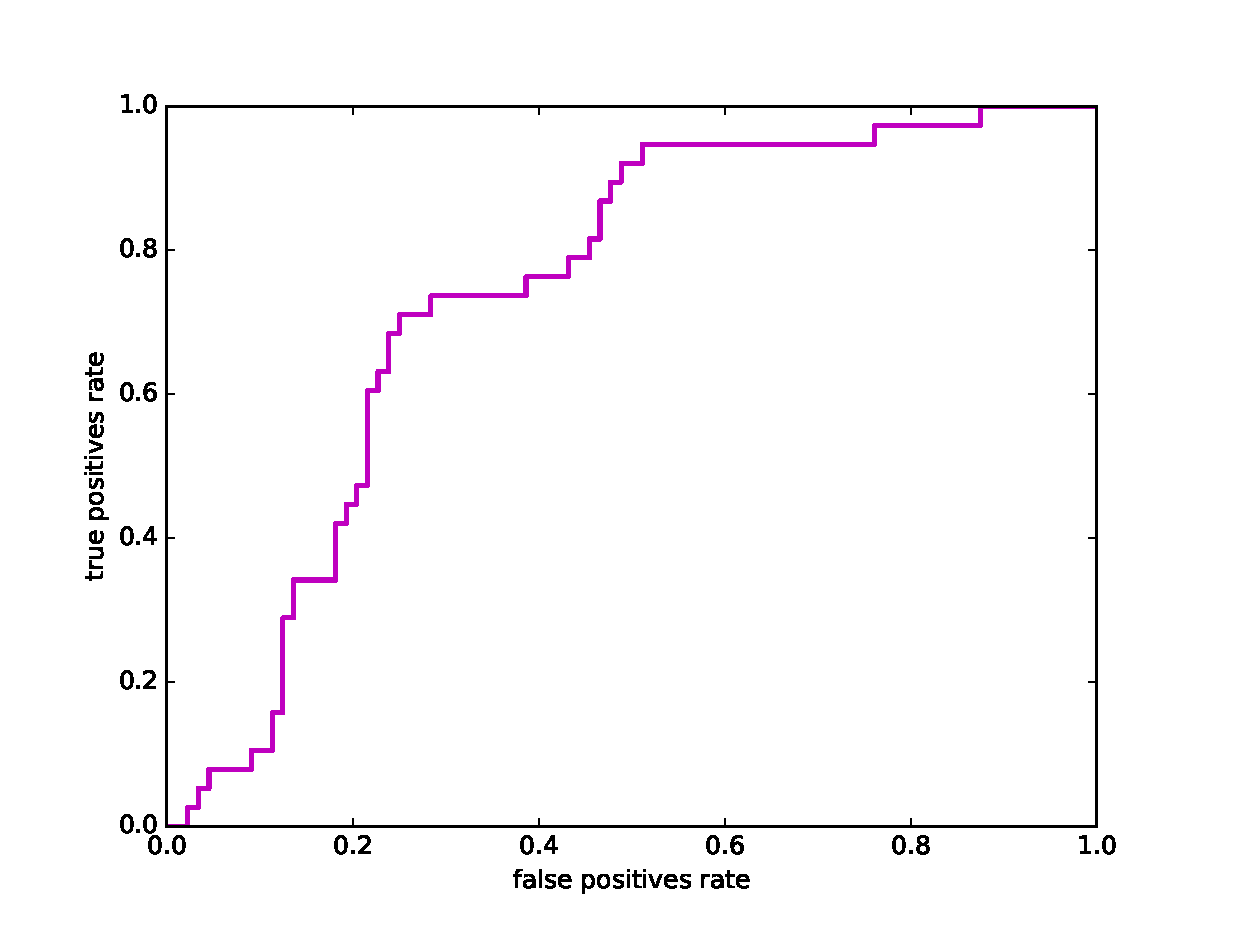
\includegraphics[width= 0.6\textwidth]{plot_roc_lupus_roc_.eps}
		%			\caption{roc curve for models of Line 5 of Table \ref{table:exp_res}.}
		\caption{ROC curve. AUC score is 0.74}
		\label{fig:lupus_roc}
\end{figure}

\begin{itemize}
	\item Results considered promising by medical experts.
	\item Improvable when more data will be available.
\end{itemize}

\end{frame}


 

 \chapter{Conclusion}
  
TODO


% \chapter{Some results}
%   \section{Vanishing gradient solutions}
%   In section \ref{vanishing_sec} were established some weak bounds on the weight matrix $\mat{W}^{rec}$ whose crossing entails the arising of
the vanishing gradient problem.

It would be nice to find some lower bounds on the weight matrix which don't allow an exponential decay of long term components. However since activation
functions can all have zero value, we cannot establish any lower bound different from zero.

However what we are really interested in is the cost of the paths which cross \textit{active} neurons because, structurally, \textit{switched off} neurons don't
contribute to the gradient. Formally we define


\begin{defn}{Active neuron}
A neuron $j$ is said to be active if $$\sigma(a_j)>\tau$$
 
\end{defn}






To overcame this problem we return to the previously introduced graph formulation where we consider each component 
$\frac{\partial \vec{a}_i^t}{\partial \vec{a}_j^k}$ as the sum path cost.



\begin{equation} 
\frac{\partial \vec{a}_i^t}{\partial \vec{a}_j^k} = \sum_{q\in P(j)} \sum_{l \in P(q)} \hdots \sum_{h : i \in P(h)} w_{qj} \hdots w_{jh} \cdot \sigma'(a_j^k)\sigma'(a_q^{k+1}) \hdots \sigma'(a_i^{t-1})
\label{expanded_mem}
\end{equation}

\appendix
\chapter{Notation}

Let $F:\mathbb{R}^N \rightarrow \mathbb{R^M}$ be defined by
\begin{equation}
F(\vec{x}) = (f_1(\vec{x}),f_2(\vec{x}),\cdots,f_M(\vec{x}))) \text{    for some  } f_i:\mathbb{R}^N \rightarrow \mathbb{R}
\end{equation}

\begin{defn}[Derivative with respect to a vector]
 We define the derivative of $F(x(\vec{w}))$ with respect to a vector $\vec{w}$ of $p$ elements as the $M \times p$ matrix
\begin{equation}
\frac{\partial F}{\partial \vec{w}} \triangleq
\begin{bmatrix}
   \frac{\partial f_1}{\partial \vec{w}_1}    & \frac{\partial f_1}{\partial \vec{w}_2}                & \cdots      & \cdots       & \frac{\partial f_1}{\partial \vec{w}_p}  \\
   \frac{\partial f_2}{\partial \vec{w}_1}    & \frac{\partial f_2}{\partial \vec{w}_2}                & \cdots      & \cdots       & \frac{\partial f_2}{\partial \vec{w}_p}  \\
   \vdots                & \vdots           & \vdots      & \vdots       &\vdots\\
   \frac{\partial f_M}{\partial \vec{w}_1}    & \frac{\partial f_M}{\partial \vec{w}_2}                & \cdots      & \cdots       & \frac{\partial f_M}{\partial \vec{w}_p}
\end{bmatrix}
\end{equation}
\end{defn}


\begin{defn}[Derivative with respect to a matrix]
We define the derivative of $F(x(\mat{W}))$ with respect to a vector $\mat{W}$, being $W_j$ the $j^{th}$ column of a $p\times m$ matrix $W$ as the $M\times (p \cdot m )$ matrix:
\begin{equation}
\frac{\partial F}{\partial \mat{W}} \triangleq
\left[
\begin{array}{c|c|c|c}
\frac{\partial F}{W_1} & \frac{\partial F}{W_2} & \cdots & \frac{\partial F}{W_m} \\
\end{array}
\right]
\end{equation}
\end{defn}





\chapter{Details of the synthetic tasks}
\label{app:tasks}
For the sake of completeness in this appendix we report all the details on the synthetic tasks we used as benchmarks in the present thesis. It should be noted that these tasks, amongst some similar other ones, have been introduced by Hochreiter \cite{lstm} in 1991 and have been used as example of particularly difficult problem for RNNs to solve since. 

These tasks are particularly difficult because they require learning long term correlations, i.e. memory and hence are perfect to test algorithms that should be able to deal with the vanishing gradient problem. A few additions are taken from Martens\cite{hessianFree}.

\paragraph{The addition problem}
The problem consists in performing an addition between two real numbers $x_i$ and $x_j$ in $[-1,1]$ belonging to a sequence of randomly generated numbers. The difficulty in this problem is that such numbers can be arbitrarily
distant in the input sequence, so the learning net must exhibit a long term memory. More specifically the input is a sequence of pairs; each pair is composed of a real number and a marker $\in\{1,0\}$. The marker is used to select the two numbers in the sequence to add. The prediction is the last value in the output sequence, the target is $\frac{x_i+x_j}{2}$. The prediction $y$ is considered correct
if $|y-\frac{x_i+x_j}{2}| < 0.04$.

Sequences have random length, say $L$, between the minimal sequence length $T$ and $T+\frac{T}{10}$, the position of the first marker is sampled in first $\frac{L}{10}$ positions, the last marker is
instead sampled in $[\frac{4L}{10},\frac{5L}{10}]$

\paragraph{The multiplication problem}
The problem is very similar to the addition problem, here we select two numbers in the input sequences of real numbers in $[0,1]$ and we need to predict the product.

\paragraph{The XOR problem}
Again, the problem is the same as the addition one but the input are binary and we are asked to predict the XOR binary operation. This problem has been found particularly hard for both LSTM and hessian-free methods as reported in \cite{hessianFree}.

\paragraph{The temporal order problem}
The input sequences are composed of $T$ randomly chosen symbols in $\{a,b,c,d\}$ except for two randomly selected positions for which the symbols are sampled in $\{x,y\}$.
The task is to predict the relative order of the two special symbols, that is $\{xx,xy,yx,yy\}$. A variant of the task is to use three special symbols instead of two.
Again, the difficulty of the problem is the possibly distance from the special symbols whose relative order is to be detected. 



\newpage
% \nocite{*}		 % Mostra in bibliografia anche gli oggetti non citati 
\bibliography{biblio}{}
\bibliographystyle{plain}


\end{document}     